\documentclass[twoside]{book}

% Packages required by doxygen
\usepackage{fixltx2e}
\usepackage{calc}
\usepackage{doxygen}
\usepackage[export]{adjustbox} % also loads graphicx
\usepackage{graphicx}
\usepackage[utf8]{inputenc}
\usepackage{makeidx}
\usepackage{multicol}
\usepackage{multirow}
\PassOptionsToPackage{warn}{textcomp}
\usepackage{textcomp}
\usepackage[nointegrals]{wasysym}
\usepackage[table]{xcolor}

% NLS support packages
\usepackage{hfont}

% Font selection
\usepackage[T1]{fontenc}
\usepackage[scaled=.90]{helvet}
\usepackage{courier}
\usepackage{amssymb}
\usepackage{sectsty}
\renewcommand{\familydefault}{\sfdefault}
\allsectionsfont{%
  \fontseries{bc}\selectfont%
  \color{darkgray}%
}
\renewcommand{\DoxyLabelFont}{%
  \fontseries{bc}\selectfont%
  \color{darkgray}%
}
\newcommand{\+}{\discretionary{\mbox{\scriptsize$\hookleftarrow$}}{}{}}

% Page & text layout
\usepackage{geometry}
\geometry{%
  a4paper,%
  top=2.5cm,%
  bottom=2.5cm,%
  left=2.5cm,%
  right=2.5cm%
}
\tolerance=750
\hfuzz=15pt
\hbadness=750
\setlength{\emergencystretch}{15pt}
\setlength{\parindent}{0cm}
\setlength{\parskip}{3ex plus 2ex minus 2ex}
\makeatletter
\renewcommand{\paragraph}{%
  \@startsection{paragraph}{4}{0ex}{-1.0ex}{1.0ex}{%
    \normalfont\normalsize\bfseries\SS@parafont%
  }%
}
\renewcommand{\subparagraph}{%
  \@startsection{subparagraph}{5}{0ex}{-1.0ex}{1.0ex}{%
    \normalfont\normalsize\bfseries\SS@subparafont%
  }%
}
\makeatother

% Headers & footers
\usepackage{fancyhdr}
\pagestyle{fancyplain}
\fancyhead[LE]{\fancyplain{}{\bfseries\thepage}}
\fancyhead[CE]{\fancyplain{}{}}
\fancyhead[RE]{\fancyplain{}{\bfseries\leftmark}}
\fancyhead[LO]{\fancyplain{}{\bfseries\rightmark}}
\fancyhead[CO]{\fancyplain{}{}}
\fancyhead[RO]{\fancyplain{}{\bfseries\thepage}}
\fancyfoot[LE]{\fancyplain{}{}}
\fancyfoot[CE]{\fancyplain{}{}}
\fancyfoot[RE]{\fancyplain{}{\bfseries\scriptsize 다음에 의해 생성됨 \+:  Doxygen }}
\fancyfoot[LO]{\fancyplain{}{\bfseries\scriptsize 다음에 의해 생성됨 \+:  Doxygen }}
\fancyfoot[CO]{\fancyplain{}{}}
\fancyfoot[RO]{\fancyplain{}{}}
\renewcommand{\footrulewidth}{0.4pt}
\renewcommand{\chaptermark}[1]{%
  \markboth{#1}{}%
}
\renewcommand{\sectionmark}[1]{%
  \markright{\thesection\ #1}%
}

% Indices & bibliography
\usepackage{natbib}
\usepackage[titles]{tocloft}
\setcounter{tocdepth}{3}
\setcounter{secnumdepth}{5}
\makeindex

% Hyperlinks (required, but should be loaded last)
\usepackage{ifpdf}
\ifpdf
  \usepackage[pdftex,pagebackref=true]{hyperref}
\else
  \usepackage[ps2pdf,pagebackref=true]{hyperref}
\fi
\hypersetup{%
  colorlinks=true,%
  linkcolor=blue,%
  citecolor=blue,%
  unicode%
}

% Custom commands
\newcommand{\clearemptydoublepage}{%
  \newpage{\pagestyle{empty}\cleardoublepage}%
}

\usepackage{caption}
\captionsetup{labelsep=space,justification=centering,font={bf},singlelinecheck=off,skip=4pt,position=top}

%===== C O N T E N T S =====

\begin{document}

% Titlepage & ToC
\hypersetup{pageanchor=false,
             bookmarksnumbered=true,
             pdfencoding=unicode
            }
\pagenumbering{alph}
\begin{titlepage}
\vspace*{7cm}
\begin{center}%
{\Large M\+N\+L\+\_\+\+D3D }\\
\vspace*{1cm}
{\large 다음에 의해 생성됨 \+:  Doxygen 1.8.13}\\
\end{center}
\end{titlepage}
\clearemptydoublepage
\pagenumbering{roman}
\tableofcontents
\clearemptydoublepage
\pagenumbering{arabic}
\hypersetup{pageanchor=true}

%--- Begin generated contents ---
\chapter{Title}
\label{index}\hypertarget{index}{}Hello 안녕 한글이 써지나? 홀롤로롤ㄹ로$\sim$ 
\chapter{헬로월드}
\label{_xED_x97_xAC_xEB_xA1_x9C_xEC_x9B_x94_xEB_x93_x9C}
\Hypertarget{_xED_x97_xAC_xEB_xA1_x9C_xEC_x9B_x94_xEB_x93_x9C}
릴레이티드 페이지가 나오쉽니까 
\chapter{네임스페이스 색인}
\section{네임스페이스 목록}
다음은 모든 네임스페이스에 대한 목록입니다. (간략한 설명만을 보여줍니다) \+:\begin{DoxyCompactList}
\item\contentsline{section}{\hyperlink{namespace_m_n_l}{M\+NL} }{\pageref{namespace_m_n_l}}{}
\item\contentsline{section}{\hyperlink{namespace_m_n_l_1_1_mn_log}{M\+N\+L\+::\+Mn\+Log} }{\pageref{namespace_m_n_l_1_1_mn_log}}{}
\end{DoxyCompactList}

\chapter{계통도 색인}
\section{클래스 계통도}
이 상속 목록은 완전하진 않지만 알파벳순으로 대략적으로 정렬되어있습니다.\+:\begin{DoxyCompactList}
\item \contentsline{section}{M\+NL\+:\+:Mn\+Resource\+Pool\+:\+:\+\_\+\+Bone\+Data}{\pageref{struct_m_n_l_1_1_mn_resource_pool_1_1___bone_data}}{}
\item \contentsline{section}{M\+NL\+:\+:Mn\+Skinned\+Mesh\+Renderer\+:\+:\+\_\+\+Bone\+Palette\+Buffer\+Type}{\pageref{struct_m_n_l_1_1_mn_skinned_mesh_renderer_1_1___bone_palette_buffer_type}}{}
\item \contentsline{section}{M\+NL\+:\+:Mn\+Mesh\+Renderer\+:\+:\+\_\+\+Light\+Buffer\+Type}{\pageref{struct_m_n_l_1_1_mn_mesh_renderer_1_1___light_buffer_type}}{}
\item \contentsline{section}{M\+NL\+:\+:Mn\+Skinned\+Mesh\+Renderer\+:\+:\+\_\+\+Light\+Buffer\+Type}{\pageref{struct_m_n_l_1_1_mn_skinned_mesh_renderer_1_1___light_buffer_type}}{}
\item \contentsline{section}{M\+NL\+:\+:Mn\+Mesh\+Renderer\+:\+:\+\_\+\+Material\+Buffer\+Type}{\pageref{struct_m_n_l_1_1_mn_mesh_renderer_1_1___material_buffer_type}}{}
\item \contentsline{section}{M\+NL\+:\+:Mn\+Skinned\+Mesh\+Renderer\+:\+:\+\_\+\+Material\+Buffer\+Type}{\pageref{struct_m_n_l_1_1_mn_skinned_mesh_renderer_1_1___material_buffer_type}}{}
\item \contentsline{section}{M\+NL\+:\+:Mn\+Resource\+Pool\+:\+:\+\_\+\+Memory\+Chunk}{\pageref{struct_m_n_l_1_1_mn_resource_pool_1_1___memory_chunk}}{}
\item \contentsline{section}{M\+NL\+:\+:Mn\+Resource\+Pool\+:\+:\+\_\+\+Model\+Package}{\pageref{struct_m_n_l_1_1_mn_resource_pool_1_1___model_package}}{}
\item \contentsline{section}{M\+NL\+:\+:Mn\+Mesh\+Renderer\+:\+:\+\_\+\+View\+Projection\+Buffer\+Type}{\pageref{struct_m_n_l_1_1_mn_mesh_renderer_1_1___view_projection_buffer_type}}{}
\item \contentsline{section}{M\+NL\+:\+:Mn\+Skinned\+Mesh\+Renderer\+:\+:\+\_\+\+View\+Projection\+Buffer\+Type}{\pageref{struct_m_n_l_1_1_mn_skinned_mesh_renderer_1_1___view_projection_buffer_type}}{}
\item \contentsline{section}{M\+NL\+:\+:Mn\+Mesh\+Renderer\+:\+:\+\_\+\+World\+Buffer\+Type}{\pageref{struct_m_n_l_1_1_mn_mesh_renderer_1_1___world_buffer_type}}{}
\item \contentsline{section}{M\+NL\+:\+:Mn\+Skinned\+Mesh\+Renderer\+:\+:\+\_\+\+World\+Buffer\+Type}{\pageref{struct_m_n_l_1_1_mn_skinned_mesh_renderer_1_1___world_buffer_type}}{}
\item \contentsline{section}{M\+NL\+:\+:Mn\+Bone}{\pageref{class_m_n_l_1_1_mn_bone}}{}
\item \contentsline{section}{M\+NL\+:\+:Mn\+Bone\+Animation}{\pageref{class_m_n_l_1_1_mn_bone_animation}}{}
\item \contentsline{section}{M\+NL\+:\+:Mn\+Bone\+Animation\+Element}{\pageref{class_m_n_l_1_1_mn_bone_animation_element}}{}
\item \contentsline{section}{M\+NL\+:\+:Mn\+Bone\+Animation\+Key\+Frame}{\pageref{struct_m_n_l_1_1_mn_bone_animation_key_frame}}{}
\item \contentsline{section}{M\+NL\+:\+:Mn\+Bone\+Animation\+Tracker}{\pageref{class_m_n_l_1_1_mn_bone_animation_tracker}}{}
\item \contentsline{section}{M\+NL\+:\+:Mn\+Camera}{\pageref{class_m_n_l_1_1_mn_camera}}{}
\item \contentsline{section}{M\+NL\+:\+:Mn\+Constant\+Buffer}{\pageref{class_m_n_l_1_1_mn_constant_buffer}}{}
\item \contentsline{section}{M\+NL\+:\+:Mn\+Constant\+Buffer\+Type}{\pageref{class_m_n_l_1_1_mn_constant_buffer_type}}{}
\item \contentsline{section}{M\+NL\+:\+:Mn\+Constant\+Element}{\pageref{class_m_n_l_1_1_mn_constant_element}}{}
\item \contentsline{section}{M\+NL\+:\+:Mn\+Custom\+Vertex\+Type}{\pageref{class_m_n_l_1_1_mn_custom_vertex_type}}{}
\begin{DoxyCompactList}
\item \contentsline{section}{M\+NL\+:\+:Mn\+Mesh\+Vertex\+Type}{\pageref{class_m_n_l_1_1_mn_mesh_vertex_type}}{}
\item \contentsline{section}{M\+NL\+:\+:Mn\+Skinned\+Mesh\+Vertex\+Type}{\pageref{class_m_n_l_1_1_mn_skinned_mesh_vertex_type}}{}
\end{DoxyCompactList}
\item \contentsline{section}{M\+NL\+:\+:Mn\+D3\+D\+Device}{\pageref{class_m_n_l_1_1_mn_d3_d_device}}{}
\item \contentsline{section}{M\+NL\+:\+:Mn\+Depth\+Stencil\+Buffer}{\pageref{class_m_n_l_1_1_mn_depth_stencil_buffer}}{}
\item \contentsline{section}{M\+NL\+:\+:Mn\+Depth\+Stencil\+State}{\pageref{class_m_n_l_1_1_mn_depth_stencil_state}}{}
\item \contentsline{section}{M\+NL\+:\+:Mn\+Display\+Device}{\pageref{class_m_n_l_1_1_mn_display_device}}{}
\item \contentsline{section}{M\+NL\+:\+:Mn\+Display\+Mode}{\pageref{struct_m_n_l_1_1_mn_display_mode}}{}
\item \contentsline{section}{M\+NL\+:\+:Mn\+Gpu\+Buffer}{\pageref{class_m_n_l_1_1_mn_gpu_buffer}}{}
\item \contentsline{section}{M\+NL\+:\+:Mn\+Hardware}{\pageref{class_m_n_l_1_1_mn_hardware}}{}
\item \contentsline{section}{M\+NL\+:\+:Mn\+Index\+Buffer}{\pageref{class_m_n_l_1_1_mn_index_buffer}}{}
\item \contentsline{section}{M\+NL\+:\+:Mn\+Input\+Element}{\pageref{class_m_n_l_1_1_mn_input_element}}{}
\item \contentsline{section}{M\+NL\+:\+:Mn\+Input\+Layout}{\pageref{class_m_n_l_1_1_mn_input_layout}}{}
\item \contentsline{section}{M\+NL\+:\+:Mn\+Light\+Source}{\pageref{class_m_n_l_1_1_mn_light_source}}{}
\item \contentsline{section}{M\+NL\+:\+:Mn\+Material}{\pageref{class_m_n_l_1_1_mn_material}}{}
\item \contentsline{section}{M\+NL\+:\+:Mn\+Matrix\+Palette}{\pageref{class_m_n_l_1_1_mn_matrix_palette}}{}
\item \contentsline{section}{M\+NL\+:\+:Mn\+Mesh}{\pageref{class_m_n_l_1_1_mn_mesh}}{}
\begin{DoxyCompactList}
\item \contentsline{section}{M\+NL\+:\+:Mn\+Skinned\+Mesh}{\pageref{class_m_n_l_1_1_mn_skinned_mesh}}{}
\item \contentsline{section}{M\+NL\+:\+:Mn\+Static\+Mesh}{\pageref{class_m_n_l_1_1_mn_static_mesh}}{}
\end{DoxyCompactList}
\item \contentsline{section}{M\+NL\+:\+:Mn\+Mesh\+Data}{\pageref{class_m_n_l_1_1_mn_mesh_data}}{}
\item \contentsline{section}{M\+NL\+:\+:Mn\+Mesh\+Texture}{\pageref{class_m_n_l_1_1_mn_mesh_texture}}{}
\item \contentsline{section}{M\+NL\+:\+:Mn\+Mesh\+Texture\+Combination}{\pageref{class_m_n_l_1_1_mn_mesh_texture_combination}}{}
\item \contentsline{section}{M\+NL\+:\+:Mn\+Pixel\+Shader}{\pageref{class_m_n_l_1_1_mn_pixel_shader}}{}
\item \contentsline{section}{M\+NL\+:\+:Mn\+Rasterizer\+State}{\pageref{class_m_n_l_1_1_mn_rasterizer_state}}{}
\item \contentsline{section}{M\+NL\+:\+:Mn\+Render\+A\+PI}{\pageref{class_m_n_l_1_1_mn_render_a_p_i}}{}
\item \contentsline{section}{M\+NL\+:\+:Mn\+Renderer}{\pageref{class_m_n_l_1_1_mn_renderer}}{}
\begin{DoxyCompactList}
\item \contentsline{section}{M\+NL\+:\+:Mn\+Mesh\+Renderer}{\pageref{class_m_n_l_1_1_mn_mesh_renderer}}{}
\item \contentsline{section}{M\+NL\+:\+:Mn\+Skinned\+Mesh\+Renderer}{\pageref{class_m_n_l_1_1_mn_skinned_mesh_renderer}}{}
\end{DoxyCompactList}
\item \contentsline{section}{M\+NL\+:\+:Mn\+Render\+Target\+View}{\pageref{class_m_n_l_1_1_mn_render_target_view}}{}
\item \contentsline{section}{M\+NL\+:\+:Mn\+Render\+Window}{\pageref{class_m_n_l_1_1_mn_render_window}}{}
\item \contentsline{section}{M\+NL\+:\+:Mn\+Resource\+Pool}{\pageref{class_m_n_l_1_1_mn_resource_pool}}{}
\item \contentsline{section}{M\+NL\+:\+:Mn\+Sampler\+State}{\pageref{class_m_n_l_1_1_mn_sampler_state}}{}
\item \contentsline{section}{M\+NL\+:\+:Mn\+Shader\+Path}{\pageref{class_m_n_l_1_1_mn_shader_path}}{}
\begin{DoxyCompactList}
\item \contentsline{section}{M\+NL\+:\+:Mn\+Shader\+Path\+Instance}{\pageref{class_m_n_l_1_1_mn_shader_path_instance}}{}
\begin{DoxyCompactList}
\item \contentsline{section}{M\+NL\+:\+:Basic\+Shader\+Path}{\pageref{class_m_n_l_1_1_basic_shader_path}}{}
\item \contentsline{section}{M\+NL\+:\+:Skinned\+Mesh\+Shader\+Path}{\pageref{class_m_n_l_1_1_skinned_mesh_shader_path}}{}
\end{DoxyCompactList}
\end{DoxyCompactList}
\item \contentsline{section}{M\+NL\+:\+:Mn\+Skeleton}{\pageref{class_m_n_l_1_1_mn_skeleton}}{}
\item \contentsline{section}{M\+NL\+:\+:Mn\+Static\+Mesh\+Vertex}{\pageref{struct_m_n_l_1_1_mn_static_mesh_vertex}}{}
\item \contentsline{section}{M\+NL\+:\+:Mn\+Sub\+Mesh}{\pageref{struct_m_n_l_1_1_mn_sub_mesh}}{}
\item \contentsline{section}{M\+NL\+:\+:Mn\+Swap\+Chain}{\pageref{class_m_n_l_1_1_mn_swap_chain}}{}
\item \contentsline{section}{M\+NL\+:\+:Mn\+Texture2D}{\pageref{class_m_n_l_1_1_mn_texture2_d}}{}
\item \contentsline{section}{M\+NL\+:\+:Mn\+Time}{\pageref{class_m_n_l_1_1_mn_time}}{}
\item \contentsline{section}{M\+NL\+:\+:Mn\+Timer}{\pageref{class_m_n_l_1_1_mn_timer}}{}
\item \contentsline{section}{M\+NL\+:\+:Mn\+Vertex\+Buffer}{\pageref{class_m_n_l_1_1_mn_vertex_buffer}}{}
\item \contentsline{section}{M\+NL\+:\+:Mn\+Vertex\+Shader}{\pageref{class_m_n_l_1_1_mn_vertex_shader}}{}
\item \contentsline{section}{M\+NL\+:\+:Mn\+Video\+Adapter}{\pageref{class_m_n_l_1_1_mn_video_adapter}}{}
\item \contentsline{section}{M\+NL\+:\+:Mn\+Viewport}{\pageref{class_m_n_l_1_1_mn_viewport}}{}
\item \contentsline{section}{M\+NL\+:\+:Mn\+Window}{\pageref{class_m_n_l_1_1_mn_window}}{}
\end{DoxyCompactList}

\chapter{클래스 색인}
\section{클래스 목록}
다음은 클래스, 구조체, 공용체 그리고 인터페이스들입니다. (간략한 설명만을 보여줍니다) \+:\begin{DoxyCompactList}
\item\contentsline{section}{\hyperlink{struct_m_n_l_1_1_mn_resource_pool_1_1___bone_data}{M\+N\+L\+::\+Mn\+Resource\+Pool\+::\+\_\+\+Bone\+Data} }{\pageref{struct_m_n_l_1_1_mn_resource_pool_1_1___bone_data}}{}
\item\contentsline{section}{\hyperlink{struct_m_n_l_1_1_mn_skinned_mesh_renderer_1_1___bone_palette_buffer_type}{M\+N\+L\+::\+Mn\+Skinned\+Mesh\+Renderer\+::\+\_\+\+Bone\+Palette\+Buffer\+Type} }{\pageref{struct_m_n_l_1_1_mn_skinned_mesh_renderer_1_1___bone_palette_buffer_type}}{}
\item\contentsline{section}{\hyperlink{struct_m_n_l_1_1_mn_mesh_renderer_1_1___light_buffer_type}{M\+N\+L\+::\+Mn\+Mesh\+Renderer\+::\+\_\+\+Light\+Buffer\+Type} }{\pageref{struct_m_n_l_1_1_mn_mesh_renderer_1_1___light_buffer_type}}{}
\item\contentsline{section}{\hyperlink{struct_m_n_l_1_1_mn_skinned_mesh_renderer_1_1___light_buffer_type}{M\+N\+L\+::\+Mn\+Skinned\+Mesh\+Renderer\+::\+\_\+\+Light\+Buffer\+Type} }{\pageref{struct_m_n_l_1_1_mn_skinned_mesh_renderer_1_1___light_buffer_type}}{}
\item\contentsline{section}{\hyperlink{struct_m_n_l_1_1_mn_mesh_renderer_1_1___material_buffer_type}{M\+N\+L\+::\+Mn\+Mesh\+Renderer\+::\+\_\+\+Material\+Buffer\+Type} }{\pageref{struct_m_n_l_1_1_mn_mesh_renderer_1_1___material_buffer_type}}{}
\item\contentsline{section}{\hyperlink{struct_m_n_l_1_1_mn_skinned_mesh_renderer_1_1___material_buffer_type}{M\+N\+L\+::\+Mn\+Skinned\+Mesh\+Renderer\+::\+\_\+\+Material\+Buffer\+Type} }{\pageref{struct_m_n_l_1_1_mn_skinned_mesh_renderer_1_1___material_buffer_type}}{}
\item\contentsline{section}{\hyperlink{struct_m_n_l_1_1_mn_resource_pool_1_1___memory_chunk}{M\+N\+L\+::\+Mn\+Resource\+Pool\+::\+\_\+\+Memory\+Chunk} }{\pageref{struct_m_n_l_1_1_mn_resource_pool_1_1___memory_chunk}}{}
\item\contentsline{section}{\hyperlink{struct_m_n_l_1_1_mn_resource_pool_1_1___model_package}{M\+N\+L\+::\+Mn\+Resource\+Pool\+::\+\_\+\+Model\+Package} }{\pageref{struct_m_n_l_1_1_mn_resource_pool_1_1___model_package}}{}
\item\contentsline{section}{\hyperlink{struct_m_n_l_1_1_mn_mesh_renderer_1_1___view_projection_buffer_type}{M\+N\+L\+::\+Mn\+Mesh\+Renderer\+::\+\_\+\+View\+Projection\+Buffer\+Type} }{\pageref{struct_m_n_l_1_1_mn_mesh_renderer_1_1___view_projection_buffer_type}}{}
\item\contentsline{section}{\hyperlink{struct_m_n_l_1_1_mn_skinned_mesh_renderer_1_1___view_projection_buffer_type}{M\+N\+L\+::\+Mn\+Skinned\+Mesh\+Renderer\+::\+\_\+\+View\+Projection\+Buffer\+Type} }{\pageref{struct_m_n_l_1_1_mn_skinned_mesh_renderer_1_1___view_projection_buffer_type}}{}
\item\contentsline{section}{\hyperlink{struct_m_n_l_1_1_mn_mesh_renderer_1_1___world_buffer_type}{M\+N\+L\+::\+Mn\+Mesh\+Renderer\+::\+\_\+\+World\+Buffer\+Type} }{\pageref{struct_m_n_l_1_1_mn_mesh_renderer_1_1___world_buffer_type}}{}
\item\contentsline{section}{\hyperlink{struct_m_n_l_1_1_mn_skinned_mesh_renderer_1_1___world_buffer_type}{M\+N\+L\+::\+Mn\+Skinned\+Mesh\+Renderer\+::\+\_\+\+World\+Buffer\+Type} }{\pageref{struct_m_n_l_1_1_mn_skinned_mesh_renderer_1_1___world_buffer_type}}{}
\item\contentsline{section}{\hyperlink{class_m_n_l_1_1_basic_shader_path}{M\+N\+L\+::\+Basic\+Shader\+Path} }{\pageref{class_m_n_l_1_1_basic_shader_path}}{}
\item\contentsline{section}{\hyperlink{class_m_n_l_1_1_mn_bone}{M\+N\+L\+::\+Mn\+Bone} }{\pageref{class_m_n_l_1_1_mn_bone}}{}
\item\contentsline{section}{\hyperlink{class_m_n_l_1_1_mn_bone_animation}{M\+N\+L\+::\+Mn\+Bone\+Animation} }{\pageref{class_m_n_l_1_1_mn_bone_animation}}{}
\item\contentsline{section}{\hyperlink{class_m_n_l_1_1_mn_bone_animation_element}{M\+N\+L\+::\+Mn\+Bone\+Animation\+Element} }{\pageref{class_m_n_l_1_1_mn_bone_animation_element}}{}
\item\contentsline{section}{\hyperlink{struct_m_n_l_1_1_mn_bone_animation_key_frame}{M\+N\+L\+::\+Mn\+Bone\+Animation\+Key\+Frame} }{\pageref{struct_m_n_l_1_1_mn_bone_animation_key_frame}}{}
\item\contentsline{section}{\hyperlink{class_m_n_l_1_1_mn_bone_animation_tracker}{M\+N\+L\+::\+Mn\+Bone\+Animation\+Tracker} }{\pageref{class_m_n_l_1_1_mn_bone_animation_tracker}}{}
\item\contentsline{section}{\hyperlink{class_m_n_l_1_1_mn_camera}{M\+N\+L\+::\+Mn\+Camera} }{\pageref{class_m_n_l_1_1_mn_camera}}{}
\item\contentsline{section}{\hyperlink{class_m_n_l_1_1_mn_constant_buffer}{M\+N\+L\+::\+Mn\+Constant\+Buffer} }{\pageref{class_m_n_l_1_1_mn_constant_buffer}}{}
\item\contentsline{section}{\hyperlink{class_m_n_l_1_1_mn_constant_buffer_type}{M\+N\+L\+::\+Mn\+Constant\+Buffer\+Type} }{\pageref{class_m_n_l_1_1_mn_constant_buffer_type}}{}
\item\contentsline{section}{\hyperlink{class_m_n_l_1_1_mn_constant_element}{M\+N\+L\+::\+Mn\+Constant\+Element} }{\pageref{class_m_n_l_1_1_mn_constant_element}}{}
\item\contentsline{section}{\hyperlink{class_m_n_l_1_1_mn_custom_vertex_type}{M\+N\+L\+::\+Mn\+Custom\+Vertex\+Type} }{\pageref{class_m_n_l_1_1_mn_custom_vertex_type}}{}
\item\contentsline{section}{\hyperlink{class_m_n_l_1_1_mn_d3_d_device}{M\+N\+L\+::\+Mn\+D3\+D\+Device} \\*D\+Irect\+X11 디바이스와 디바이스 컨텍스트를 생성, 관리한다 }{\pageref{class_m_n_l_1_1_mn_d3_d_device}}{}
\item\contentsline{section}{\hyperlink{class_m_n_l_1_1_mn_depth_stencil_buffer}{M\+N\+L\+::\+Mn\+Depth\+Stencil\+Buffer} }{\pageref{class_m_n_l_1_1_mn_depth_stencil_buffer}}{}
\item\contentsline{section}{\hyperlink{class_m_n_l_1_1_mn_depth_stencil_state}{M\+N\+L\+::\+Mn\+Depth\+Stencil\+State} }{\pageref{class_m_n_l_1_1_mn_depth_stencil_state}}{}
\item\contentsline{section}{\hyperlink{class_m_n_l_1_1_mn_display_device}{M\+N\+L\+::\+Mn\+Display\+Device} \\*디스플레이 장치의 디스플레이 모드 정보를 얻어와 저장한다 }{\pageref{class_m_n_l_1_1_mn_display_device}}{}
\item\contentsline{section}{\hyperlink{struct_m_n_l_1_1_mn_display_mode}{M\+N\+L\+::\+Mn\+Display\+Mode} \\*디스플레이 모드 정보를 담고있다 }{\pageref{struct_m_n_l_1_1_mn_display_mode}}{}
\item\contentsline{section}{\hyperlink{class_m_n_l_1_1_mn_gpu_buffer}{M\+N\+L\+::\+Mn\+Gpu\+Buffer} }{\pageref{class_m_n_l_1_1_mn_gpu_buffer}}{}
\item\contentsline{section}{\hyperlink{class_m_n_l_1_1_mn_hardware}{M\+N\+L\+::\+Mn\+Hardware} \\*비디오 어댑터 및 디스플레이 장치 관리 }{\pageref{class_m_n_l_1_1_mn_hardware}}{}
\item\contentsline{section}{\hyperlink{class_m_n_l_1_1_mn_index_buffer}{M\+N\+L\+::\+Mn\+Index\+Buffer} }{\pageref{class_m_n_l_1_1_mn_index_buffer}}{}
\item\contentsline{section}{\hyperlink{class_m_n_l_1_1_mn_input_element}{M\+N\+L\+::\+Mn\+Input\+Element} }{\pageref{class_m_n_l_1_1_mn_input_element}}{}
\item\contentsline{section}{\hyperlink{class_m_n_l_1_1_mn_input_layout}{M\+N\+L\+::\+Mn\+Input\+Layout} }{\pageref{class_m_n_l_1_1_mn_input_layout}}{}
\item\contentsline{section}{\hyperlink{class_m_n_l_1_1_mn_light_source}{M\+N\+L\+::\+Mn\+Light\+Source} }{\pageref{class_m_n_l_1_1_mn_light_source}}{}
\item\contentsline{section}{\hyperlink{class_m_n_l_1_1_mn_material}{M\+N\+L\+::\+Mn\+Material} }{\pageref{class_m_n_l_1_1_mn_material}}{}
\item\contentsline{section}{\hyperlink{class_m_n_l_1_1_mn_matrix_palette}{M\+N\+L\+::\+Mn\+Matrix\+Palette} }{\pageref{class_m_n_l_1_1_mn_matrix_palette}}{}
\item\contentsline{section}{\hyperlink{class_m_n_l_1_1_mn_mesh}{M\+N\+L\+::\+Mn\+Mesh} }{\pageref{class_m_n_l_1_1_mn_mesh}}{}
\item\contentsline{section}{\hyperlink{class_m_n_l_1_1_mn_mesh_data}{M\+N\+L\+::\+Mn\+Mesh\+Data} }{\pageref{class_m_n_l_1_1_mn_mesh_data}}{}
\item\contentsline{section}{\hyperlink{class_m_n_l_1_1_mn_mesh_renderer}{M\+N\+L\+::\+Mn\+Mesh\+Renderer} }{\pageref{class_m_n_l_1_1_mn_mesh_renderer}}{}
\item\contentsline{section}{\hyperlink{class_m_n_l_1_1_mn_mesh_texture}{M\+N\+L\+::\+Mn\+Mesh\+Texture} }{\pageref{class_m_n_l_1_1_mn_mesh_texture}}{}
\item\contentsline{section}{\hyperlink{class_m_n_l_1_1_mn_mesh_texture_combination}{M\+N\+L\+::\+Mn\+Mesh\+Texture\+Combination} }{\pageref{class_m_n_l_1_1_mn_mesh_texture_combination}}{}
\item\contentsline{section}{\hyperlink{class_m_n_l_1_1_mn_mesh_vertex_type}{M\+N\+L\+::\+Mn\+Mesh\+Vertex\+Type} }{\pageref{class_m_n_l_1_1_mn_mesh_vertex_type}}{}
\item\contentsline{section}{\hyperlink{class_m_n_l_1_1_mn_pixel_shader}{M\+N\+L\+::\+Mn\+Pixel\+Shader} }{\pageref{class_m_n_l_1_1_mn_pixel_shader}}{}
\item\contentsline{section}{\hyperlink{class_m_n_l_1_1_mn_rasterizer_state}{M\+N\+L\+::\+Mn\+Rasterizer\+State} }{\pageref{class_m_n_l_1_1_mn_rasterizer_state}}{}
\item\contentsline{section}{\hyperlink{class_m_n_l_1_1_mn_render_a_p_i}{M\+N\+L\+::\+Mn\+Render\+A\+PI} \\*비디오 장치와 상호작용 하는 모든 인터페이스를 지니는 객체 }{\pageref{class_m_n_l_1_1_mn_render_a_p_i}}{}
\item\contentsline{section}{\hyperlink{class_m_n_l_1_1_mn_renderer}{M\+N\+L\+::\+Mn\+Renderer} }{\pageref{class_m_n_l_1_1_mn_renderer}}{}
\item\contentsline{section}{\hyperlink{class_m_n_l_1_1_mn_render_target_view}{M\+N\+L\+::\+Mn\+Render\+Target\+View} }{\pageref{class_m_n_l_1_1_mn_render_target_view}}{}
\item\contentsline{section}{\hyperlink{class_m_n_l_1_1_mn_render_window}{M\+N\+L\+::\+Mn\+Render\+Window} }{\pageref{class_m_n_l_1_1_mn_render_window}}{}
\item\contentsline{section}{\hyperlink{class_m_n_l_1_1_mn_resource_pool}{M\+N\+L\+::\+Mn\+Resource\+Pool} }{\pageref{class_m_n_l_1_1_mn_resource_pool}}{}
\item\contentsline{section}{\hyperlink{class_m_n_l_1_1_mn_sampler_state}{M\+N\+L\+::\+Mn\+Sampler\+State} }{\pageref{class_m_n_l_1_1_mn_sampler_state}}{}
\item\contentsline{section}{\hyperlink{class_m_n_l_1_1_mn_shader_path}{M\+N\+L\+::\+Mn\+Shader\+Path} }{\pageref{class_m_n_l_1_1_mn_shader_path}}{}
\item\contentsline{section}{\hyperlink{class_m_n_l_1_1_mn_shader_path_instance}{M\+N\+L\+::\+Mn\+Shader\+Path\+Instance} }{\pageref{class_m_n_l_1_1_mn_shader_path_instance}}{}
\item\contentsline{section}{\hyperlink{class_m_n_l_1_1_mn_skeleton}{M\+N\+L\+::\+Mn\+Skeleton} }{\pageref{class_m_n_l_1_1_mn_skeleton}}{}
\item\contentsline{section}{\hyperlink{class_m_n_l_1_1_mn_skinned_mesh}{M\+N\+L\+::\+Mn\+Skinned\+Mesh} }{\pageref{class_m_n_l_1_1_mn_skinned_mesh}}{}
\item\contentsline{section}{\hyperlink{class_m_n_l_1_1_mn_skinned_mesh_renderer}{M\+N\+L\+::\+Mn\+Skinned\+Mesh\+Renderer} }{\pageref{class_m_n_l_1_1_mn_skinned_mesh_renderer}}{}
\item\contentsline{section}{\hyperlink{class_m_n_l_1_1_mn_skinned_mesh_vertex_type}{M\+N\+L\+::\+Mn\+Skinned\+Mesh\+Vertex\+Type} }{\pageref{class_m_n_l_1_1_mn_skinned_mesh_vertex_type}}{}
\item\contentsline{section}{\hyperlink{class_m_n_l_1_1_mn_static_mesh}{M\+N\+L\+::\+Mn\+Static\+Mesh} }{\pageref{class_m_n_l_1_1_mn_static_mesh}}{}
\item\contentsline{section}{\hyperlink{struct_m_n_l_1_1_mn_static_mesh_vertex}{M\+N\+L\+::\+Mn\+Static\+Mesh\+Vertex} }{\pageref{struct_m_n_l_1_1_mn_static_mesh_vertex}}{}
\item\contentsline{section}{\hyperlink{struct_m_n_l_1_1_mn_sub_mesh}{M\+N\+L\+::\+Mn\+Sub\+Mesh} }{\pageref{struct_m_n_l_1_1_mn_sub_mesh}}{}
\item\contentsline{section}{\hyperlink{class_m_n_l_1_1_mn_swap_chain}{M\+N\+L\+::\+Mn\+Swap\+Chain} }{\pageref{class_m_n_l_1_1_mn_swap_chain}}{}
\item\contentsline{section}{\hyperlink{class_m_n_l_1_1_mn_texture2_d}{M\+N\+L\+::\+Mn\+Texture2D} }{\pageref{class_m_n_l_1_1_mn_texture2_d}}{}
\item\contentsline{section}{\hyperlink{class_m_n_l_1_1_mn_time}{M\+N\+L\+::\+Mn\+Time} }{\pageref{class_m_n_l_1_1_mn_time}}{}
\item\contentsline{section}{\hyperlink{class_m_n_l_1_1_mn_timer}{M\+N\+L\+::\+Mn\+Timer} }{\pageref{class_m_n_l_1_1_mn_timer}}{}
\item\contentsline{section}{\hyperlink{class_m_n_l_1_1_mn_vertex_buffer}{M\+N\+L\+::\+Mn\+Vertex\+Buffer} }{\pageref{class_m_n_l_1_1_mn_vertex_buffer}}{}
\item\contentsline{section}{\hyperlink{class_m_n_l_1_1_mn_vertex_shader}{M\+N\+L\+::\+Mn\+Vertex\+Shader} }{\pageref{class_m_n_l_1_1_mn_vertex_shader}}{}
\item\contentsline{section}{\hyperlink{class_m_n_l_1_1_mn_video_adapter}{M\+N\+L\+::\+Mn\+Video\+Adapter} \\*비디오 어댑터의 정보와 디스플레이 장치들을 저장한다 }{\pageref{class_m_n_l_1_1_mn_video_adapter}}{}
\item\contentsline{section}{\hyperlink{class_m_n_l_1_1_mn_viewport}{M\+N\+L\+::\+Mn\+Viewport} }{\pageref{class_m_n_l_1_1_mn_viewport}}{}
\item\contentsline{section}{\hyperlink{class_m_n_l_1_1_mn_window}{M\+N\+L\+::\+Mn\+Window} }{\pageref{class_m_n_l_1_1_mn_window}}{}
\item\contentsline{section}{\hyperlink{class_m_n_l_1_1_skinned_mesh_shader_path}{M\+N\+L\+::\+Skinned\+Mesh\+Shader\+Path} }{\pageref{class_m_n_l_1_1_skinned_mesh_shader_path}}{}
\end{DoxyCompactList}

\chapter{파일 색인}
\section{파일 목록}
다음은 모든 파일에 대한 목록입니다. (간략한 설명만을 보여줍니다) \+:\begin{DoxyCompactList}
\item\contentsline{section}{\hyperlink{_basic_shader_path_8cpp}{Basic\+Shader\+Path.\+cpp} }{\pageref{_basic_shader_path_8cpp}}{}
\item\contentsline{section}{\hyperlink{_basic_shader_path_8h}{Basic\+Shader\+Path.\+h} }{\pageref{_basic_shader_path_8h}}{}
\item\contentsline{section}{\hyperlink{main_8cpp}{main.\+cpp} }{\pageref{main_8cpp}}{}
\item\contentsline{section}{\hyperlink{_skinned_mesh_shader_path_8cpp}{Skinned\+Mesh\+Shader\+Path.\+cpp} }{\pageref{_skinned_mesh_shader_path_8cpp}}{}
\item\contentsline{section}{\hyperlink{_skinned_mesh_shader_path_8h}{Skinned\+Mesh\+Shader\+Path.\+h} }{\pageref{_skinned_mesh_shader_path_8h}}{}
\item\contentsline{section}{Core/\hyperlink{_mn_constant_buffer_8cpp}{Mn\+Constant\+Buffer.\+cpp} }{\pageref{_mn_constant_buffer_8cpp}}{}
\item\contentsline{section}{Core/\hyperlink{_mn_constant_buffer_8h}{Mn\+Constant\+Buffer.\+h} }{\pageref{_mn_constant_buffer_8h}}{}
\item\contentsline{section}{Core/\hyperlink{_mn_constant_buffer_type_8cpp}{Mn\+Constant\+Buffer\+Type.\+cpp} }{\pageref{_mn_constant_buffer_type_8cpp}}{}
\item\contentsline{section}{Core/\hyperlink{_mn_constant_buffer_type_8h}{Mn\+Constant\+Buffer\+Type.\+h} }{\pageref{_mn_constant_buffer_type_8h}}{}
\item\contentsline{section}{Core/\hyperlink{_mn_constant_element_8cpp}{Mn\+Constant\+Element.\+cpp} }{\pageref{_mn_constant_element_8cpp}}{}
\item\contentsline{section}{Core/\hyperlink{_mn_constant_element_8h}{Mn\+Constant\+Element.\+h} }{\pageref{_mn_constant_element_8h}}{}
\item\contentsline{section}{Core/\hyperlink{_mn_custom_vertex_type_8cpp}{Mn\+Custom\+Vertex\+Type.\+cpp} }{\pageref{_mn_custom_vertex_type_8cpp}}{}
\item\contentsline{section}{Core/\hyperlink{_mn_custom_vertex_type_8h}{Mn\+Custom\+Vertex\+Type.\+h} }{\pageref{_mn_custom_vertex_type_8h}}{}
\item\contentsline{section}{Core/\hyperlink{_mn_d3_d_device_8cpp}{Mn\+D3\+D\+Device.\+cpp} }{\pageref{_mn_d3_d_device_8cpp}}{}
\item\contentsline{section}{Core/\hyperlink{_mn_d3_d_device_8h}{Mn\+D3\+D\+Device.\+h} }{\pageref{_mn_d3_d_device_8h}}{}
\item\contentsline{section}{Core/\hyperlink{_mn_depth_stencil_buffer_8cpp}{Mn\+Depth\+Stencil\+Buffer.\+cpp} }{\pageref{_mn_depth_stencil_buffer_8cpp}}{}
\item\contentsline{section}{Core/\hyperlink{_mn_depth_stencil_buffer_8h}{Mn\+Depth\+Stencil\+Buffer.\+h} }{\pageref{_mn_depth_stencil_buffer_8h}}{}
\item\contentsline{section}{Core/\hyperlink{_mn_depth_stencil_state_8cpp}{Mn\+Depth\+Stencil\+State.\+cpp} }{\pageref{_mn_depth_stencil_state_8cpp}}{}
\item\contentsline{section}{Core/\hyperlink{_mn_depth_stencil_state_8h}{Mn\+Depth\+Stencil\+State.\+h} }{\pageref{_mn_depth_stencil_state_8h}}{}
\item\contentsline{section}{Core/\hyperlink{_mn_display_device_8cpp}{Mn\+Display\+Device.\+cpp} }{\pageref{_mn_display_device_8cpp}}{}
\item\contentsline{section}{Core/\hyperlink{_mn_display_device_8h}{Mn\+Display\+Device.\+h} }{\pageref{_mn_display_device_8h}}{}
\item\contentsline{section}{Core/\hyperlink{_mn_gpu_buffer_8cpp}{Mn\+Gpu\+Buffer.\+cpp} }{\pageref{_mn_gpu_buffer_8cpp}}{}
\item\contentsline{section}{Core/\hyperlink{_mn_gpu_buffer_8h}{Mn\+Gpu\+Buffer.\+h} }{\pageref{_mn_gpu_buffer_8h}}{}
\item\contentsline{section}{Core/\hyperlink{_mn_hardware_8cpp}{Mn\+Hardware.\+cpp} }{\pageref{_mn_hardware_8cpp}}{}
\item\contentsline{section}{Core/\hyperlink{_mn_hardware_8h}{Mn\+Hardware.\+h} }{\pageref{_mn_hardware_8h}}{}
\item\contentsline{section}{Core/\hyperlink{_mn_index_buffer_8cpp}{Mn\+Index\+Buffer.\+cpp} }{\pageref{_mn_index_buffer_8cpp}}{}
\item\contentsline{section}{Core/\hyperlink{_mn_index_buffer_8h}{Mn\+Index\+Buffer.\+h} }{\pageref{_mn_index_buffer_8h}}{}
\item\contentsline{section}{Core/\hyperlink{_mn_input_element_8cpp}{Mn\+Input\+Element.\+cpp} }{\pageref{_mn_input_element_8cpp}}{}
\item\contentsline{section}{Core/\hyperlink{_mn_input_element_8h}{Mn\+Input\+Element.\+h} }{\pageref{_mn_input_element_8h}}{}
\item\contentsline{section}{Core/\hyperlink{_mn_input_layout_8cpp}{Mn\+Input\+Layout.\+cpp} }{\pageref{_mn_input_layout_8cpp}}{}
\item\contentsline{section}{Core/\hyperlink{_mn_input_layout_8h}{Mn\+Input\+Layout.\+h} }{\pageref{_mn_input_layout_8h}}{}
\item\contentsline{section}{Core/\hyperlink{_m_n_l___core_8h}{M\+N\+L\+\_\+\+Core.\+h} }{\pageref{_m_n_l___core_8h}}{}
\item\contentsline{section}{Core/\hyperlink{_mn_log_8cpp}{Mn\+Log.\+cpp} }{\pageref{_mn_log_8cpp}}{}
\item\contentsline{section}{Core/\hyperlink{_mn_log_8h}{Mn\+Log.\+h} }{\pageref{_mn_log_8h}}{}
\item\contentsline{section}{Core/\hyperlink{_mn_macros_8h}{Mn\+Macros.\+h} }{\pageref{_mn_macros_8h}}{}
\item\contentsline{section}{Core/\hyperlink{_mn_pixel_shader_8cpp}{Mn\+Pixel\+Shader.\+cpp} }{\pageref{_mn_pixel_shader_8cpp}}{}
\item\contentsline{section}{Core/\hyperlink{_mn_pixel_shader_8h}{Mn\+Pixel\+Shader.\+h} }{\pageref{_mn_pixel_shader_8h}}{}
\item\contentsline{section}{Core/\hyperlink{_mn_rasterizer_state_8cpp}{Mn\+Rasterizer\+State.\+cpp} }{\pageref{_mn_rasterizer_state_8cpp}}{}
\item\contentsline{section}{Core/\hyperlink{_mn_rasterizer_state_8h}{Mn\+Rasterizer\+State.\+h} }{\pageref{_mn_rasterizer_state_8h}}{}
\item\contentsline{section}{Core/\hyperlink{_mn_render_a_p_i_8cpp}{Mn\+Render\+A\+P\+I.\+cpp} }{\pageref{_mn_render_a_p_i_8cpp}}{}
\item\contentsline{section}{Core/\hyperlink{_mn_render_a_p_i_8h}{Mn\+Render\+A\+P\+I.\+h} }{\pageref{_mn_render_a_p_i_8h}}{}
\item\contentsline{section}{Core/\hyperlink{_mn_render_target_view_8cpp}{Mn\+Render\+Target\+View.\+cpp} }{\pageref{_mn_render_target_view_8cpp}}{}
\item\contentsline{section}{Core/\hyperlink{_mn_render_target_view_8h}{Mn\+Render\+Target\+View.\+h} }{\pageref{_mn_render_target_view_8h}}{}
\item\contentsline{section}{Core/\hyperlink{_mn_sampler_state_8cpp}{Mn\+Sampler\+State.\+cpp} }{\pageref{_mn_sampler_state_8cpp}}{}
\item\contentsline{section}{Core/\hyperlink{_mn_sampler_state_8h}{Mn\+Sampler\+State.\+h} }{\pageref{_mn_sampler_state_8h}}{}
\item\contentsline{section}{Core/\hyperlink{_mn_swap_chain_8cpp}{Mn\+Swap\+Chain.\+cpp} }{\pageref{_mn_swap_chain_8cpp}}{}
\item\contentsline{section}{Core/\hyperlink{_mn_swap_chain_8h}{Mn\+Swap\+Chain.\+h} }{\pageref{_mn_swap_chain_8h}}{}
\item\contentsline{section}{Core/\hyperlink{_mn_texture2_d_8cpp}{Mn\+Texture2\+D.\+cpp} }{\pageref{_mn_texture2_d_8cpp}}{}
\item\contentsline{section}{Core/\hyperlink{_mn_texture2_d_8h}{Mn\+Texture2\+D.\+h} }{\pageref{_mn_texture2_d_8h}}{}
\item\contentsline{section}{Core/\hyperlink{_mn_typedefs_8h}{Mn\+Typedefs.\+h} }{\pageref{_mn_typedefs_8h}}{}
\item\contentsline{section}{Core/\hyperlink{_mn_vertex_buffer_8cpp}{Mn\+Vertex\+Buffer.\+cpp} }{\pageref{_mn_vertex_buffer_8cpp}}{}
\item\contentsline{section}{Core/\hyperlink{_mn_vertex_buffer_8h}{Mn\+Vertex\+Buffer.\+h} }{\pageref{_mn_vertex_buffer_8h}}{}
\item\contentsline{section}{Core/\hyperlink{_mn_vertex_shader_8cpp}{Mn\+Vertex\+Shader.\+cpp} }{\pageref{_mn_vertex_shader_8cpp}}{}
\item\contentsline{section}{Core/\hyperlink{_mn_vertex_shader_8h}{Mn\+Vertex\+Shader.\+h} }{\pageref{_mn_vertex_shader_8h}}{}
\item\contentsline{section}{Core/\hyperlink{_mn_video_adapter_8cpp}{Mn\+Video\+Adapter.\+cpp} }{\pageref{_mn_video_adapter_8cpp}}{}
\item\contentsline{section}{Core/\hyperlink{_mn_video_adapter_8h}{Mn\+Video\+Adapter.\+h} }{\pageref{_mn_video_adapter_8h}}{}
\item\contentsline{section}{Core/\hyperlink{_mn_viewport_8cpp}{Mn\+Viewport.\+cpp} }{\pageref{_mn_viewport_8cpp}}{}
\item\contentsline{section}{Core/\hyperlink{_mn_viewport_8h}{Mn\+Viewport.\+h} }{\pageref{_mn_viewport_8h}}{}
\item\contentsline{section}{Core/\hyperlink{_mn_window_8cpp}{Mn\+Window.\+cpp} }{\pageref{_mn_window_8cpp}}{}
\item\contentsline{section}{Core/\hyperlink{_mn_window_8h}{Mn\+Window.\+h} }{\pageref{_mn_window_8h}}{}
\item\contentsline{section}{Render/\hyperlink{_mn_bone_8cpp}{Mn\+Bone.\+cpp} }{\pageref{_mn_bone_8cpp}}{}
\item\contentsline{section}{Render/\hyperlink{_mn_bone_8h}{Mn\+Bone.\+h} }{\pageref{_mn_bone_8h}}{}
\item\contentsline{section}{Render/\hyperlink{_mn_bone_animation_8cpp}{Mn\+Bone\+Animation.\+cpp} }{\pageref{_mn_bone_animation_8cpp}}{}
\item\contentsline{section}{Render/\hyperlink{_mn_bone_animation_8h}{Mn\+Bone\+Animation.\+h} }{\pageref{_mn_bone_animation_8h}}{}
\item\contentsline{section}{Render/\hyperlink{_mn_bone_animation_element_8cpp}{Mn\+Bone\+Animation\+Element.\+cpp} }{\pageref{_mn_bone_animation_element_8cpp}}{}
\item\contentsline{section}{Render/\hyperlink{_mn_bone_animation_element_8h}{Mn\+Bone\+Animation\+Element.\+h} }{\pageref{_mn_bone_animation_element_8h}}{}
\item\contentsline{section}{Render/\hyperlink{_mn_bone_animation_tracker_8cpp}{Mn\+Bone\+Animation\+Tracker.\+cpp} }{\pageref{_mn_bone_animation_tracker_8cpp}}{}
\item\contentsline{section}{Render/\hyperlink{_mn_bone_animation_tracker_8h}{Mn\+Bone\+Animation\+Tracker.\+h} }{\pageref{_mn_bone_animation_tracker_8h}}{}
\item\contentsline{section}{Render/\hyperlink{_mn_camera_8cpp}{Mn\+Camera.\+cpp} }{\pageref{_mn_camera_8cpp}}{}
\item\contentsline{section}{Render/\hyperlink{_mn_camera_8h}{Mn\+Camera.\+h} }{\pageref{_mn_camera_8h}}{}
\item\contentsline{section}{Render/\hyperlink{_m_n_l___render_8h}{M\+N\+L\+\_\+\+Render.\+h} }{\pageref{_m_n_l___render_8h}}{}
\item\contentsline{section}{Render/\hyperlink{_mn_light_source_8cpp}{Mn\+Light\+Source.\+cpp} }{\pageref{_mn_light_source_8cpp}}{}
\item\contentsline{section}{Render/\hyperlink{_mn_light_source_8h}{Mn\+Light\+Source.\+h} }{\pageref{_mn_light_source_8h}}{}
\item\contentsline{section}{Render/\hyperlink{_mn_material_8cpp}{Mn\+Material.\+cpp} }{\pageref{_mn_material_8cpp}}{}
\item\contentsline{section}{Render/\hyperlink{_mn_material_8h}{Mn\+Material.\+h} }{\pageref{_mn_material_8h}}{}
\item\contentsline{section}{Render/\hyperlink{_mn_matrix_palette_8cpp}{Mn\+Matrix\+Palette.\+cpp} }{\pageref{_mn_matrix_palette_8cpp}}{}
\item\contentsline{section}{Render/\hyperlink{_mn_matrix_palette_8h}{Mn\+Matrix\+Palette.\+h} }{\pageref{_mn_matrix_palette_8h}}{}
\item\contentsline{section}{Render/\hyperlink{_mn_mesh_8cpp}{Mn\+Mesh.\+cpp} }{\pageref{_mn_mesh_8cpp}}{}
\item\contentsline{section}{Render/\hyperlink{_mn_mesh_8h}{Mn\+Mesh.\+h} }{\pageref{_mn_mesh_8h}}{}
\item\contentsline{section}{Render/\hyperlink{_mn_mesh_data_8cpp}{Mn\+Mesh\+Data.\+cpp} }{\pageref{_mn_mesh_data_8cpp}}{}
\item\contentsline{section}{Render/\hyperlink{_mn_mesh_data_8h}{Mn\+Mesh\+Data.\+h} }{\pageref{_mn_mesh_data_8h}}{}
\item\contentsline{section}{Render/\hyperlink{_mn_mesh_renderer_8cpp}{Mn\+Mesh\+Renderer.\+cpp} }{\pageref{_mn_mesh_renderer_8cpp}}{}
\item\contentsline{section}{Render/\hyperlink{_mn_mesh_renderer_8h}{Mn\+Mesh\+Renderer.\+h} }{\pageref{_mn_mesh_renderer_8h}}{}
\item\contentsline{section}{Render/\hyperlink{_mn_mesh_texture_8cpp}{Mn\+Mesh\+Texture.\+cpp} }{\pageref{_mn_mesh_texture_8cpp}}{}
\item\contentsline{section}{Render/\hyperlink{_mn_mesh_texture_8h}{Mn\+Mesh\+Texture.\+h} }{\pageref{_mn_mesh_texture_8h}}{}
\item\contentsline{section}{Render/\hyperlink{_mn_mesh_texture_combination_8cpp}{Mn\+Mesh\+Texture\+Combination.\+cpp} }{\pageref{_mn_mesh_texture_combination_8cpp}}{}
\item\contentsline{section}{Render/\hyperlink{_mn_mesh_texture_combination_8h}{Mn\+Mesh\+Texture\+Combination.\+h} }{\pageref{_mn_mesh_texture_combination_8h}}{}
\item\contentsline{section}{Render/\hyperlink{_mn_mesh_vertex_type_8cpp}{Mn\+Mesh\+Vertex\+Type.\+cpp} }{\pageref{_mn_mesh_vertex_type_8cpp}}{}
\item\contentsline{section}{Render/\hyperlink{_mn_mesh_vertex_type_8h}{Mn\+Mesh\+Vertex\+Type.\+h} }{\pageref{_mn_mesh_vertex_type_8h}}{}
\item\contentsline{section}{Render/\hyperlink{_mn_renderer_8cpp}{Mn\+Renderer.\+cpp} }{\pageref{_mn_renderer_8cpp}}{}
\item\contentsline{section}{Render/\hyperlink{_mn_renderer_8h}{Mn\+Renderer.\+h} }{\pageref{_mn_renderer_8h}}{}
\item\contentsline{section}{Render/\hyperlink{_mn_render_window_8cpp}{Mn\+Render\+Window.\+cpp} }{\pageref{_mn_render_window_8cpp}}{}
\item\contentsline{section}{Render/\hyperlink{_mn_render_window_8h}{Mn\+Render\+Window.\+h} }{\pageref{_mn_render_window_8h}}{}
\item\contentsline{section}{Render/\hyperlink{_mn_shader_path_8cpp}{Mn\+Shader\+Path.\+cpp} }{\pageref{_mn_shader_path_8cpp}}{}
\item\contentsline{section}{Render/\hyperlink{_mn_shader_path_8h}{Mn\+Shader\+Path.\+h} }{\pageref{_mn_shader_path_8h}}{}
\item\contentsline{section}{Render/\hyperlink{_mn_shader_path_instance_8cpp}{Mn\+Shader\+Path\+Instance.\+cpp} }{\pageref{_mn_shader_path_instance_8cpp}}{}
\item\contentsline{section}{Render/\hyperlink{_mn_shader_path_instance_8h}{Mn\+Shader\+Path\+Instance.\+h} }{\pageref{_mn_shader_path_instance_8h}}{}
\item\contentsline{section}{Render/\hyperlink{_mn_skeleton_8cpp}{Mn\+Skeleton.\+cpp} }{\pageref{_mn_skeleton_8cpp}}{}
\item\contentsline{section}{Render/\hyperlink{_mn_skeleton_8h}{Mn\+Skeleton.\+h} }{\pageref{_mn_skeleton_8h}}{}
\item\contentsline{section}{Render/\hyperlink{_mn_skinned_mesh_8cpp}{Mn\+Skinned\+Mesh.\+cpp} }{\pageref{_mn_skinned_mesh_8cpp}}{}
\item\contentsline{section}{Render/\hyperlink{_mn_skinned_mesh_8h}{Mn\+Skinned\+Mesh.\+h} }{\pageref{_mn_skinned_mesh_8h}}{}
\item\contentsline{section}{Render/\hyperlink{_mn_skinned_mesh_renderer_8cpp}{Mn\+Skinned\+Mesh\+Renderer.\+cpp} }{\pageref{_mn_skinned_mesh_renderer_8cpp}}{}
\item\contentsline{section}{Render/\hyperlink{_mn_skinned_mesh_renderer_8h}{Mn\+Skinned\+Mesh\+Renderer.\+h} }{\pageref{_mn_skinned_mesh_renderer_8h}}{}
\item\contentsline{section}{Render/\hyperlink{_mn_skinned_mesh_vertex_type_8cpp}{Mn\+Skinned\+Mesh\+Vertex\+Type.\+cpp} }{\pageref{_mn_skinned_mesh_vertex_type_8cpp}}{}
\item\contentsline{section}{Render/\hyperlink{_mn_skinned_mesh_vertex_type_8h}{Mn\+Skinned\+Mesh\+Vertex\+Type.\+h} }{\pageref{_mn_skinned_mesh_vertex_type_8h}}{}
\item\contentsline{section}{Render/\hyperlink{_mn_static_mesh_8cpp}{Mn\+Static\+Mesh.\+cpp} }{\pageref{_mn_static_mesh_8cpp}}{}
\item\contentsline{section}{Render/\hyperlink{_mn_static_mesh_8h}{Mn\+Static\+Mesh.\+h} }{\pageref{_mn_static_mesh_8h}}{}
\item\contentsline{section}{Utility/\hyperlink{_m_n_l___utility_8h}{M\+N\+L\+\_\+\+Utility.\+h} }{\pageref{_m_n_l___utility_8h}}{}
\item\contentsline{section}{Utility/\hyperlink{_mn_resource_pool_8cpp}{Mn\+Resource\+Pool.\+cpp} }{\pageref{_mn_resource_pool_8cpp}}{}
\item\contentsline{section}{Utility/\hyperlink{_mn_resource_pool_8h}{Mn\+Resource\+Pool.\+h} }{\pageref{_mn_resource_pool_8h}}{}
\item\contentsline{section}{Utility/\hyperlink{_mn_timer_8cpp}{Mn\+Timer.\+cpp} }{\pageref{_mn_timer_8cpp}}{}
\item\contentsline{section}{Utility/\hyperlink{_mn_timer_8h}{Mn\+Timer.\+h} }{\pageref{_mn_timer_8h}}{}
\end{DoxyCompactList}

\chapter{네임스페이스 문서화}
\hypertarget{namespace_m_n_l}{}\section{M\+NL 네임스페이스 참조}
\label{namespace_m_n_l}\index{M\+NL@{M\+NL}}
\subsection*{네임스페이스}
\begin{DoxyCompactItemize}
\item 
 \hyperlink{namespace_m_n_l_1_1_mn_log}{Mn\+Log}
\end{DoxyCompactItemize}
\subsection*{클래스}
\begin{DoxyCompactItemize}
\item 
class \hyperlink{class_m_n_l_1_1_basic_shader_path}{Basic\+Shader\+Path}
\item 
class \hyperlink{class_m_n_l_1_1_mn_bone}{Mn\+Bone}
\item 
class \hyperlink{class_m_n_l_1_1_mn_bone_animation}{Mn\+Bone\+Animation}
\item 
class \hyperlink{class_m_n_l_1_1_mn_bone_animation_element}{Mn\+Bone\+Animation\+Element}
\item 
struct \hyperlink{struct_m_n_l_1_1_mn_bone_animation_key_frame}{Mn\+Bone\+Animation\+Key\+Frame}
\item 
class \hyperlink{class_m_n_l_1_1_mn_bone_animation_tracker}{Mn\+Bone\+Animation\+Tracker}
\item 
class \hyperlink{class_m_n_l_1_1_mn_camera}{Mn\+Camera}
\item 
class \hyperlink{class_m_n_l_1_1_mn_constant_buffer}{Mn\+Constant\+Buffer}
\item 
class \hyperlink{class_m_n_l_1_1_mn_constant_buffer_type}{Mn\+Constant\+Buffer\+Type}
\item 
class \hyperlink{class_m_n_l_1_1_mn_constant_element}{Mn\+Constant\+Element}
\item 
class \hyperlink{class_m_n_l_1_1_mn_custom_vertex_type}{Mn\+Custom\+Vertex\+Type}
\item 
class \hyperlink{class_m_n_l_1_1_mn_d3_d_device}{Mn\+D3\+D\+Device}
\begin{DoxyCompactList}\small\item\em D\+Irect\+X11 디바이스와 디바이스 컨텍스트를 생성, 관리한다. \end{DoxyCompactList}\item 
class \hyperlink{class_m_n_l_1_1_mn_depth_stencil_buffer}{Mn\+Depth\+Stencil\+Buffer}
\item 
class \hyperlink{class_m_n_l_1_1_mn_depth_stencil_state}{Mn\+Depth\+Stencil\+State}
\item 
class \hyperlink{class_m_n_l_1_1_mn_display_device}{Mn\+Display\+Device}
\begin{DoxyCompactList}\small\item\em 디스플레이 장치의 디스플레이 모드 정보를 얻어와 저장한다. \end{DoxyCompactList}\item 
struct \hyperlink{struct_m_n_l_1_1_mn_display_mode}{Mn\+Display\+Mode}
\begin{DoxyCompactList}\small\item\em 디스플레이 모드 정보를 담고있다. \end{DoxyCompactList}\item 
class \hyperlink{class_m_n_l_1_1_mn_gpu_buffer}{Mn\+Gpu\+Buffer}
\item 
class \hyperlink{class_m_n_l_1_1_mn_hardware}{Mn\+Hardware}
\begin{DoxyCompactList}\small\item\em 비디오 어댑터 및 디스플레이 장치 관리. \end{DoxyCompactList}\item 
class \hyperlink{class_m_n_l_1_1_mn_index_buffer}{Mn\+Index\+Buffer}
\item 
class \hyperlink{class_m_n_l_1_1_mn_input_element}{Mn\+Input\+Element}
\item 
class \hyperlink{class_m_n_l_1_1_mn_input_layout}{Mn\+Input\+Layout}
\item 
class \hyperlink{class_m_n_l_1_1_mn_light_source}{Mn\+Light\+Source}
\item 
class \hyperlink{class_m_n_l_1_1_mn_material}{Mn\+Material}
\item 
class \hyperlink{class_m_n_l_1_1_mn_matrix_palette}{Mn\+Matrix\+Palette}
\item 
class \hyperlink{class_m_n_l_1_1_mn_mesh}{Mn\+Mesh}
\item 
class \hyperlink{class_m_n_l_1_1_mn_mesh_data}{Mn\+Mesh\+Data}
\item 
class \hyperlink{class_m_n_l_1_1_mn_mesh_renderer}{Mn\+Mesh\+Renderer}
\item 
class \hyperlink{class_m_n_l_1_1_mn_mesh_texture}{Mn\+Mesh\+Texture}
\item 
class \hyperlink{class_m_n_l_1_1_mn_mesh_texture_combination}{Mn\+Mesh\+Texture\+Combination}
\item 
class \hyperlink{class_m_n_l_1_1_mn_mesh_vertex_type}{Mn\+Mesh\+Vertex\+Type}
\item 
class \hyperlink{class_m_n_l_1_1_mn_pixel_shader}{Mn\+Pixel\+Shader}
\item 
class \hyperlink{class_m_n_l_1_1_mn_rasterizer_state}{Mn\+Rasterizer\+State}
\item 
class \hyperlink{class_m_n_l_1_1_mn_render_a_p_i}{Mn\+Render\+A\+PI}
\begin{DoxyCompactList}\small\item\em 비디오 장치와 상호작용 하는 모든 인터페이스를 지니는 객체 \end{DoxyCompactList}\item 
class \hyperlink{class_m_n_l_1_1_mn_renderer}{Mn\+Renderer}
\item 
class \hyperlink{class_m_n_l_1_1_mn_render_target_view}{Mn\+Render\+Target\+View}
\item 
class \hyperlink{class_m_n_l_1_1_mn_render_window}{Mn\+Render\+Window}
\item 
class \hyperlink{class_m_n_l_1_1_mn_resource_pool}{Mn\+Resource\+Pool}
\item 
class \hyperlink{class_m_n_l_1_1_mn_sampler_state}{Mn\+Sampler\+State}
\item 
class \hyperlink{class_m_n_l_1_1_mn_shader_path}{Mn\+Shader\+Path}
\item 
class \hyperlink{class_m_n_l_1_1_mn_shader_path_instance}{Mn\+Shader\+Path\+Instance}
\item 
class \hyperlink{class_m_n_l_1_1_mn_skeleton}{Mn\+Skeleton}
\item 
class \hyperlink{class_m_n_l_1_1_mn_skinned_mesh}{Mn\+Skinned\+Mesh}
\item 
class \hyperlink{class_m_n_l_1_1_mn_skinned_mesh_renderer}{Mn\+Skinned\+Mesh\+Renderer}
\item 
class \hyperlink{class_m_n_l_1_1_mn_skinned_mesh_vertex_type}{Mn\+Skinned\+Mesh\+Vertex\+Type}
\item 
class \hyperlink{class_m_n_l_1_1_mn_static_mesh}{Mn\+Static\+Mesh}
\item 
struct \hyperlink{struct_m_n_l_1_1_mn_static_mesh_vertex}{Mn\+Static\+Mesh\+Vertex}
\item 
struct \hyperlink{struct_m_n_l_1_1_mn_sub_mesh}{Mn\+Sub\+Mesh}
\item 
class \hyperlink{class_m_n_l_1_1_mn_swap_chain}{Mn\+Swap\+Chain}
\item 
class \hyperlink{class_m_n_l_1_1_mn_texture2_d}{Mn\+Texture2D}
\item 
class \hyperlink{class_m_n_l_1_1_mn_time}{Mn\+Time}
\item 
class \hyperlink{class_m_n_l_1_1_mn_timer}{Mn\+Timer}
\item 
class \hyperlink{class_m_n_l_1_1_mn_vertex_buffer}{Mn\+Vertex\+Buffer}
\item 
class \hyperlink{class_m_n_l_1_1_mn_vertex_shader}{Mn\+Vertex\+Shader}
\item 
class \hyperlink{class_m_n_l_1_1_mn_video_adapter}{Mn\+Video\+Adapter}
\begin{DoxyCompactList}\small\item\em 비디오 어댑터의 정보와 디스플레이 장치들을 저장한다. \end{DoxyCompactList}\item 
class \hyperlink{class_m_n_l_1_1_mn_viewport}{Mn\+Viewport}
\item 
class \hyperlink{class_m_n_l_1_1_mn_window}{Mn\+Window}
\item 
class \hyperlink{class_m_n_l_1_1_skinned_mesh_shader_path}{Skinned\+Mesh\+Shader\+Path}
\end{DoxyCompactItemize}
\subsection*{타입정의}
\begin{DoxyCompactItemize}
\item 
typedef Microsoft\+::\+W\+R\+L\+::\+Com\+Ptr$<$ I\+D3\+D11\+Device $>$ \hyperlink{namespace_m_n_l_a1eec210db8f309a4a9ac0d9658784c31}{C\+P\+D3\+D\+Device}
\item 
typedef Microsoft\+::\+W\+R\+L\+::\+Com\+Ptr$<$ I\+D3\+D11\+Device\+Context $>$ \hyperlink{namespace_m_n_l_aab3aabb6c9360e44ddc8b0bb563c2107}{C\+P\+D3\+D\+Device\+Context}
\item 
typedef Microsoft\+::\+W\+R\+L\+::\+Com\+Ptr$<$ I\+D3\+D11\+Depth\+Stencil\+State $>$ \hyperlink{namespace_m_n_l_a8209b06065c025e5d6bc2e8ee5925faf}{C\+P\+D3\+D\+Depth\+Stencil\+State}
\item 
typedef Microsoft\+::\+W\+R\+L\+::\+Com\+Ptr$<$ I\+D3\+D11\+Depth\+Stencil\+View $>$ \hyperlink{namespace_m_n_l_a12b3c209d76ede855300e637f4192a04}{C\+P\+D3\+D\+Depth\+Stencil\+View}
\item 
typedef Microsoft\+::\+W\+R\+L\+::\+Com\+Ptr$<$ I\+D3\+D11\+Rasterizer\+State $>$ \hyperlink{namespace_m_n_l_aa6c2682c64c5b58c458c36bb424f1e56}{C\+P\+D3\+D\+Rasterizer\+State}
\item 
typedef Microsoft\+::\+W\+R\+L\+::\+Com\+Ptr$<$ I\+D3\+D11\+Vertex\+Shader $>$ \hyperlink{namespace_m_n_l_a8036d713226061c4827b537821fbf79b}{C\+P\+D3\+D\+Vertex\+Shader}
\item 
typedef Microsoft\+::\+W\+R\+L\+::\+Com\+Ptr$<$ I\+D3\+D11\+Pixel\+Shader $>$ \hyperlink{namespace_m_n_l_a4d6bd408e6e19137a03728583296f12a}{C\+P\+D3\+D\+Pixel\+Shader}
\item 
typedef Microsoft\+::\+W\+R\+L\+::\+Com\+Ptr$<$ I\+D3\+D10\+Blob $>$ \hyperlink{namespace_m_n_l_a3716e3bee60c31fe1b7b5dd5a82db59a}{C\+P\+D3\+D\+Blob}
\item 
typedef Microsoft\+::\+W\+R\+L\+::\+Com\+Ptr$<$ I\+D3\+D11\+Buffer $>$ \hyperlink{namespace_m_n_l_aab9c90a8c27ac6410a9cc7cd89efeef1}{C\+P\+D3\+D\+Buffer}
\item 
typedef Microsoft\+::\+W\+R\+L\+::\+Com\+Ptr$<$ I\+D3\+D11\+Texture2D $>$ \hyperlink{namespace_m_n_l_addb538e1cbd1f443e6db5e6312487c51}{C\+P\+D3\+D\+Texture2D}
\item 
typedef Microsoft\+::\+W\+R\+L\+::\+Com\+Ptr$<$ I\+D3\+D11\+Render\+Target\+View $>$ \hyperlink{namespace_m_n_l_aa08a7c0b5ac9d877dacb57b9306b7b8c}{C\+P\+D3\+D\+Render\+Target\+View}
\item 
typedef Microsoft\+::\+W\+R\+L\+::\+Com\+Ptr$<$ I\+D3\+D11\+Sampler\+State $>$ \hyperlink{namespace_m_n_l_ae0141196161ecb3d3055523077ca3aa1}{C\+P\+D3\+D\+Sampler\+State}
\item 
typedef Microsoft\+::\+W\+R\+L\+::\+Com\+Ptr$<$ I\+D3\+D11\+Shader\+Resource\+View $>$ \hyperlink{namespace_m_n_l_a93794d93663474ff79c950ed985565aa}{C\+P\+D3\+D\+Shader\+Resource\+View}
\item 
typedef Microsoft\+::\+W\+R\+L\+::\+Com\+Ptr$<$ I\+D3\+D11\+Input\+Layout $>$ \hyperlink{namespace_m_n_l_aec7a2a132d6e72492d5feb5926d838dd}{C\+P\+D3\+D\+Input\+Layout}
\item 
typedef Microsoft\+::\+W\+R\+L\+::\+Com\+Ptr$<$ I\+D\+X\+G\+I\+Swap\+Chain $>$ \hyperlink{namespace_m_n_l_a5e8905e111c1a9d829a86fc3cc3420ec}{C\+P\+D\+X\+G\+I\+Swap\+Chain}
\item 
typedef Microsoft\+::\+W\+R\+L\+::\+Com\+Ptr$<$ I\+D\+X\+G\+I\+Factory $>$ \hyperlink{namespace_m_n_l_a8bb070ff80c5e3a874d942fbc31c22ab}{C\+P\+D\+X\+G\+I\+Factory}
\item 
typedef Microsoft\+::\+W\+R\+L\+::\+Com\+Ptr$<$ I\+D\+X\+G\+I\+Adapter $>$ \hyperlink{namespace_m_n_l_ab0e24805043a50c45364c389f8929f33}{C\+P\+D\+X\+G\+I\+Adapter}
\item 
typedef Microsoft\+::\+W\+R\+L\+::\+Com\+Ptr$<$ I\+D\+X\+G\+I\+Output $>$ \hyperlink{namespace_m_n_l_ac03add2215d9e5f2938af7887c5b09de}{C\+P\+D\+X\+G\+I\+Output}
\end{DoxyCompactItemize}
\subsection*{열거형 타입}
\begin{DoxyCompactItemize}
\item 
enum \hyperlink{namespace_m_n_l_a3f526411258a17023ecac1a36e666d42}{M\+N\+\_\+\+C\+O\+N\+S\+T\+A\+N\+T\+\_\+\+B\+U\+F\+F\+E\+R\+\_\+\+B\+E\+L\+O\+NG} \{ \hyperlink{namespace_m_n_l_a3f526411258a17023ecac1a36e666d42a622011e1ea7300991444d2168e657367}{Mn\+\_\+\+C\+O\+N\+S\+T\+A\+N\+T\+\_\+\+B\+U\+F\+F\+E\+R\+\_\+\+B\+E\+L\+O\+N\+G\+\_\+\+N\+O\+NE}, 
\hyperlink{namespace_m_n_l_a3f526411258a17023ecac1a36e666d42a11c5b064576f194422e313943d4d19c6}{M\+N\+\_\+\+C\+O\+N\+S\+T\+A\+N\+T\+\_\+\+B\+U\+F\+F\+E\+R\+\_\+\+B\+E\+L\+O\+N\+G\+\_\+\+VS}, 
\hyperlink{namespace_m_n_l_a3f526411258a17023ecac1a36e666d42ab50cc6b460a7205f8822f971a6897fa9}{M\+N\+\_\+\+C\+O\+N\+S\+T\+A\+N\+T\+\_\+\+B\+U\+F\+F\+E\+R\+\_\+\+B\+E\+L\+O\+N\+G\+\_\+\+PS}
 \}
\item 
enum \hyperlink{namespace_m_n_l_a7d0c6fcd5ada7e43f4059b8a9b4afb49}{Mn\+Constant\+Element\+Type} \{ \newline
\hyperlink{namespace_m_n_l_a7d0c6fcd5ada7e43f4059b8a9b4afb49a63259a0215999c46a1e0d42421e2c3f6}{M\+N\+\_\+\+C\+O\+N\+S\+T\+A\+N\+T\+\_\+\+E\+L\+E\+M\+E\+N\+T\+\_\+\+T\+Y\+P\+E\+\_\+\+N\+O\+NE}, 
\hyperlink{namespace_m_n_l_a7d0c6fcd5ada7e43f4059b8a9b4afb49ab5a80c7054840efdb379fb98cb1307e3}{M\+N\+\_\+\+C\+O\+N\+S\+T\+A\+N\+T\+\_\+\+E\+L\+E\+M\+E\+N\+T\+\_\+\+T\+Y\+P\+E\+\_\+\+F\+L\+O\+A\+T1}, 
\hyperlink{namespace_m_n_l_a7d0c6fcd5ada7e43f4059b8a9b4afb49a57cb21c01b95cebc8ff1be3cda3d6319}{M\+N\+\_\+\+C\+O\+N\+S\+T\+A\+N\+T\+\_\+\+E\+L\+E\+M\+E\+N\+T\+\_\+\+T\+Y\+P\+E\+\_\+\+F\+L\+O\+A\+T2}, 
\hyperlink{namespace_m_n_l_a7d0c6fcd5ada7e43f4059b8a9b4afb49a4d69f036a2972b6f553dfbdc952f997c}{M\+N\+\_\+\+C\+O\+N\+S\+T\+A\+N\+T\+\_\+\+E\+L\+E\+M\+E\+N\+T\+\_\+\+T\+Y\+P\+E\+\_\+\+F\+L\+O\+A\+T3}, 
\newline
\hyperlink{namespace_m_n_l_a7d0c6fcd5ada7e43f4059b8a9b4afb49ab87d18978e034d623b604da63717fb94}{M\+N\+\_\+\+C\+O\+N\+S\+T\+A\+N\+T\+\_\+\+E\+L\+E\+M\+E\+N\+T\+\_\+\+T\+Y\+P\+E\+\_\+\+F\+L\+O\+A\+T4}, 
\hyperlink{namespace_m_n_l_a7d0c6fcd5ada7e43f4059b8a9b4afb49a166913415b78247345fd7ec34a0c709c}{M\+N\+\_\+\+C\+O\+N\+S\+T\+A\+N\+T\+\_\+\+E\+L\+E\+M\+E\+N\+T\+\_\+\+T\+Y\+P\+E\+\_\+\+M\+A\+T\+R\+IX}, 
\hyperlink{namespace_m_n_l_a7d0c6fcd5ada7e43f4059b8a9b4afb49a4f494495e0ad8498f9c3cc367f06100f}{M\+N\+\_\+\+C\+O\+N\+S\+T\+A\+N\+T\+\_\+\+E\+L\+E\+M\+E\+N\+T\+\_\+\+T\+Y\+P\+E\+\_\+\+U\+I\+NT}
 \}
\item 
enum \hyperlink{namespace_m_n_l_a37da403537a061d6aaa45b7d30f29ac2}{M\+N\+\_\+\+C\+U\+S\+T\+O\+M\+\_\+\+V\+E\+R\+T\+E\+X\+\_\+\+F\+L\+AG} \{ \newline
\hyperlink{namespace_m_n_l_a37da403537a061d6aaa45b7d30f29ac2a7d7b0b8edbe1b8def4a32c9213678e7d}{M\+N\+\_\+\+C\+V\+F\+\_\+\+F\+L\+A\+G\+\_\+\+N\+O\+NE} = 0, 
\hyperlink{namespace_m_n_l_a37da403537a061d6aaa45b7d30f29ac2a4cf1244060eefbfda236b22fbda2c4cf}{M\+N\+\_\+\+C\+V\+F\+\_\+\+P\+O\+S\+I\+T\+I\+O\+N0} = 0x0001, 
\hyperlink{namespace_m_n_l_a37da403537a061d6aaa45b7d30f29ac2ab44d5ba8b90926e730115e3b5f0bbc58}{M\+N\+\_\+\+C\+V\+F\+\_\+\+P\+O\+S\+I\+T\+I\+O\+N1} = 0x0002, 
\hyperlink{namespace_m_n_l_a37da403537a061d6aaa45b7d30f29ac2a8f14b012f816a0c98b1718a117b87e0f}{M\+N\+\_\+\+C\+V\+F\+\_\+\+P\+O\+S\+I\+T\+I\+O\+N2} = 0x0004, 
\newline
\hyperlink{namespace_m_n_l_a37da403537a061d6aaa45b7d30f29ac2a2ec3e576e18d24b6485bfe6dae5aa63a}{M\+N\+\_\+\+C\+V\+F\+\_\+\+P\+O\+S\+I\+T\+I\+O\+N3} = 0x0008, 
\hyperlink{namespace_m_n_l_a37da403537a061d6aaa45b7d30f29ac2a151c750ae013b0097e9f7e3e85681f6b}{M\+N\+\_\+\+C\+V\+F\+\_\+\+N\+O\+R\+M\+A\+L0} = 0x0010, 
\hyperlink{namespace_m_n_l_a37da403537a061d6aaa45b7d30f29ac2a29444f3109df8a7f28ab5a6838adb6c5}{M\+N\+\_\+\+C\+V\+F\+\_\+\+N\+O\+R\+M\+A\+L1} = 0x0020, 
\hyperlink{namespace_m_n_l_a37da403537a061d6aaa45b7d30f29ac2a20560a44a544b3f8689b80bf221befbc}{M\+N\+\_\+\+C\+V\+F\+\_\+\+N\+O\+R\+M\+A\+L2} = 0x0040, 
\newline
\hyperlink{namespace_m_n_l_a37da403537a061d6aaa45b7d30f29ac2a73f4fe3fc511e61d6552c5b87ed8a38b}{M\+N\+\_\+\+C\+V\+F\+\_\+\+N\+O\+R\+M\+A\+L3} = 0x0080, 
\hyperlink{namespace_m_n_l_a37da403537a061d6aaa45b7d30f29ac2a09ee0d7c406a1a7e5913f6d621178975}{M\+N\+\_\+\+C\+V\+F\+\_\+\+T\+E\+X\+C\+O\+O\+R\+D0} = 0x0100, 
\hyperlink{namespace_m_n_l_a37da403537a061d6aaa45b7d30f29ac2ab7becd11025206819812444d62bbd092}{M\+N\+\_\+\+C\+V\+F\+\_\+\+T\+E\+X\+C\+O\+O\+R\+D1} = 0x0200, 
\hyperlink{namespace_m_n_l_a37da403537a061d6aaa45b7d30f29ac2a70802d224421f0ffb845e9cdec47652d}{M\+N\+\_\+\+C\+V\+F\+\_\+\+T\+E\+X\+C\+O\+O\+R\+D2} = 0x0400, 
\newline
\hyperlink{namespace_m_n_l_a37da403537a061d6aaa45b7d30f29ac2af8bba5b37c926fc75b892e13093c3346}{M\+N\+\_\+\+C\+V\+F\+\_\+\+T\+E\+X\+C\+O\+O\+R\+D3} = 0x0800, 
\hyperlink{namespace_m_n_l_a37da403537a061d6aaa45b7d30f29ac2a6ae04a185c157665ef96703f2ff14acd}{M\+N\+\_\+\+C\+V\+F\+\_\+\+B\+O\+N\+E\+\_\+\+I\+N\+D\+EX} = 0x1000, 
\hyperlink{namespace_m_n_l_a37da403537a061d6aaa45b7d30f29ac2a0ff3a87360c8f392bada3538477f5dec}{M\+N\+\_\+\+C\+V\+F\+\_\+\+B\+O\+N\+E\+\_\+\+W\+E\+I\+G\+HT} = 0x2000, 
\hyperlink{namespace_m_n_l_a37da403537a061d6aaa45b7d30f29ac2a49bf921871a33b21f3526c9a1a2c9671}{M\+N\+\_\+\+C\+V\+F\+\_\+\+O\+P\+T\+I\+O\+N2} = 0x4000, 
\newline
\hyperlink{namespace_m_n_l_a37da403537a061d6aaa45b7d30f29ac2a4b61871b94be7afa3cf4545778fe2234}{M\+N\+\_\+\+C\+V\+F\+\_\+\+O\+P\+T\+I\+O\+N3} = 0x8000
 \}
\item 
enum \hyperlink{namespace_m_n_l_a8605571a36b2bb477280767d71fe6f9e}{Mn\+Input\+Element\+Type} \{ \newline
\hyperlink{namespace_m_n_l_a8605571a36b2bb477280767d71fe6f9ea16f702c06e35b85077e39ce81b4e8004}{M\+N\+\_\+\+I\+N\+P\+U\+T\+\_\+\+E\+L\+E\+M\+E\+N\+T\+\_\+\+T\+Y\+P\+E\+\_\+\+N\+O\+NE}, 
\hyperlink{namespace_m_n_l_a8605571a36b2bb477280767d71fe6f9ea79ff25ed13ed363ab51080a5e49a3ce1}{M\+N\+\_\+\+I\+N\+P\+U\+T\+\_\+\+E\+L\+E\+M\+E\+N\+T\+\_\+\+T\+Y\+P\+E\+\_\+\+F\+L\+O\+A\+T1}, 
\hyperlink{namespace_m_n_l_a8605571a36b2bb477280767d71fe6f9ea306c60bed97bba07f77ff5b4766c02cb}{M\+N\+\_\+\+I\+N\+P\+U\+T\+\_\+\+E\+L\+E\+M\+E\+N\+T\+\_\+\+T\+Y\+P\+E\+\_\+\+F\+L\+O\+A\+T2}, 
\hyperlink{namespace_m_n_l_a8605571a36b2bb477280767d71fe6f9ea4d78a38c56b95c6855212c178f97d621}{M\+N\+\_\+\+I\+N\+P\+U\+T\+\_\+\+E\+L\+E\+M\+E\+N\+T\+\_\+\+T\+Y\+P\+E\+\_\+\+F\+L\+O\+A\+T3}, 
\newline
\hyperlink{namespace_m_n_l_a8605571a36b2bb477280767d71fe6f9ea37046f207cd7ff368225528152c2b760}{M\+N\+\_\+\+I\+N\+P\+U\+T\+\_\+\+E\+L\+E\+M\+E\+N\+T\+\_\+\+T\+Y\+P\+E\+\_\+\+F\+L\+O\+A\+T4}
 \}
\item 
enum \hyperlink{namespace_m_n_l_aac0b78de8bb8c872cb617ede813c113d}{M\+N\+\_\+\+L\+I\+G\+H\+T\+\_\+\+T\+Y\+PE} \{ \hyperlink{namespace_m_n_l_aac0b78de8bb8c872cb617ede813c113daae2f70c21587a6e8c7fc71a6c799975f}{M\+N\+\_\+\+L\+I\+G\+H\+T\+\_\+\+D\+I\+R\+E\+C\+T\+I\+O\+N\+AL}, 
\hyperlink{namespace_m_n_l_aac0b78de8bb8c872cb617ede813c113da7f51745230321843b3fe800eb08b3967}{M\+N\+\_\+\+L\+I\+G\+H\+T\+\_\+\+P\+O\+I\+NT}
 \}
\end{DoxyCompactItemize}


\subsection{타입정의 문서화}
\mbox{\Hypertarget{namespace_m_n_l_a3716e3bee60c31fe1b7b5dd5a82db59a}\label{namespace_m_n_l_a3716e3bee60c31fe1b7b5dd5a82db59a}} 
\index{M\+NL@{M\+NL}!C\+P\+D3\+D\+Blob@{C\+P\+D3\+D\+Blob}}
\index{C\+P\+D3\+D\+Blob@{C\+P\+D3\+D\+Blob}!M\+NL@{M\+NL}}
\subsubsection{\texorpdfstring{C\+P\+D3\+D\+Blob}{CPD3DBlob}}
{\footnotesize\ttfamily typedef Microsoft\+::\+W\+R\+L\+::\+Com\+Ptr$<$I\+D3\+D10\+Blob$>$ \hyperlink{namespace_m_n_l_a3716e3bee60c31fe1b7b5dd5a82db59a}{M\+N\+L\+::\+C\+P\+D3\+D\+Blob}}



Mn\+Typedefs.\+h 파일의 15 번째 라인에서 정의되었습니다.

\mbox{\Hypertarget{namespace_m_n_l_aab9c90a8c27ac6410a9cc7cd89efeef1}\label{namespace_m_n_l_aab9c90a8c27ac6410a9cc7cd89efeef1}} 
\index{M\+NL@{M\+NL}!C\+P\+D3\+D\+Buffer@{C\+P\+D3\+D\+Buffer}}
\index{C\+P\+D3\+D\+Buffer@{C\+P\+D3\+D\+Buffer}!M\+NL@{M\+NL}}
\subsubsection{\texorpdfstring{C\+P\+D3\+D\+Buffer}{CPD3DBuffer}}
{\footnotesize\ttfamily typedef Microsoft\+::\+W\+R\+L\+::\+Com\+Ptr$<$I\+D3\+D11\+Buffer$>$ \hyperlink{namespace_m_n_l_aab9c90a8c27ac6410a9cc7cd89efeef1}{M\+N\+L\+::\+C\+P\+D3\+D\+Buffer}}



Mn\+Typedefs.\+h 파일의 17 번째 라인에서 정의되었습니다.

\mbox{\Hypertarget{namespace_m_n_l_a8209b06065c025e5d6bc2e8ee5925faf}\label{namespace_m_n_l_a8209b06065c025e5d6bc2e8ee5925faf}} 
\index{M\+NL@{M\+NL}!C\+P\+D3\+D\+Depth\+Stencil\+State@{C\+P\+D3\+D\+Depth\+Stencil\+State}}
\index{C\+P\+D3\+D\+Depth\+Stencil\+State@{C\+P\+D3\+D\+Depth\+Stencil\+State}!M\+NL@{M\+NL}}
\subsubsection{\texorpdfstring{C\+P\+D3\+D\+Depth\+Stencil\+State}{CPD3DDepthStencilState}}
{\footnotesize\ttfamily typedef Microsoft\+::\+W\+R\+L\+::\+Com\+Ptr$<$I\+D3\+D11\+Depth\+Stencil\+State$>$ \hyperlink{namespace_m_n_l_a8209b06065c025e5d6bc2e8ee5925faf}{M\+N\+L\+::\+C\+P\+D3\+D\+Depth\+Stencil\+State}}



Mn\+Typedefs.\+h 파일의 8 번째 라인에서 정의되었습니다.

\mbox{\Hypertarget{namespace_m_n_l_a12b3c209d76ede855300e637f4192a04}\label{namespace_m_n_l_a12b3c209d76ede855300e637f4192a04}} 
\index{M\+NL@{M\+NL}!C\+P\+D3\+D\+Depth\+Stencil\+View@{C\+P\+D3\+D\+Depth\+Stencil\+View}}
\index{C\+P\+D3\+D\+Depth\+Stencil\+View@{C\+P\+D3\+D\+Depth\+Stencil\+View}!M\+NL@{M\+NL}}
\subsubsection{\texorpdfstring{C\+P\+D3\+D\+Depth\+Stencil\+View}{CPD3DDepthStencilView}}
{\footnotesize\ttfamily typedef Microsoft\+::\+W\+R\+L\+::\+Com\+Ptr$<$I\+D3\+D11\+Depth\+Stencil\+View$>$ \hyperlink{namespace_m_n_l_a12b3c209d76ede855300e637f4192a04}{M\+N\+L\+::\+C\+P\+D3\+D\+Depth\+Stencil\+View}}



Mn\+Typedefs.\+h 파일의 9 번째 라인에서 정의되었습니다.

\mbox{\Hypertarget{namespace_m_n_l_a1eec210db8f309a4a9ac0d9658784c31}\label{namespace_m_n_l_a1eec210db8f309a4a9ac0d9658784c31}} 
\index{M\+NL@{M\+NL}!C\+P\+D3\+D\+Device@{C\+P\+D3\+D\+Device}}
\index{C\+P\+D3\+D\+Device@{C\+P\+D3\+D\+Device}!M\+NL@{M\+NL}}
\subsubsection{\texorpdfstring{C\+P\+D3\+D\+Device}{CPD3DDevice}}
{\footnotesize\ttfamily typedef Microsoft\+::\+W\+R\+L\+::\+Com\+Ptr$<$I\+D3\+D11\+Device$>$ \hyperlink{namespace_m_n_l_a1eec210db8f309a4a9ac0d9658784c31}{M\+N\+L\+::\+C\+P\+D3\+D\+Device}}



Mn\+Typedefs.\+h 파일의 6 번째 라인에서 정의되었습니다.

\mbox{\Hypertarget{namespace_m_n_l_aab3aabb6c9360e44ddc8b0bb563c2107}\label{namespace_m_n_l_aab3aabb6c9360e44ddc8b0bb563c2107}} 
\index{M\+NL@{M\+NL}!C\+P\+D3\+D\+Device\+Context@{C\+P\+D3\+D\+Device\+Context}}
\index{C\+P\+D3\+D\+Device\+Context@{C\+P\+D3\+D\+Device\+Context}!M\+NL@{M\+NL}}
\subsubsection{\texorpdfstring{C\+P\+D3\+D\+Device\+Context}{CPD3DDeviceContext}}
{\footnotesize\ttfamily typedef Microsoft\+::\+W\+R\+L\+::\+Com\+Ptr$<$I\+D3\+D11\+Device\+Context$>$ \hyperlink{namespace_m_n_l_aab3aabb6c9360e44ddc8b0bb563c2107}{M\+N\+L\+::\+C\+P\+D3\+D\+Device\+Context}}



Mn\+Typedefs.\+h 파일의 7 번째 라인에서 정의되었습니다.

\mbox{\Hypertarget{namespace_m_n_l_aec7a2a132d6e72492d5feb5926d838dd}\label{namespace_m_n_l_aec7a2a132d6e72492d5feb5926d838dd}} 
\index{M\+NL@{M\+NL}!C\+P\+D3\+D\+Input\+Layout@{C\+P\+D3\+D\+Input\+Layout}}
\index{C\+P\+D3\+D\+Input\+Layout@{C\+P\+D3\+D\+Input\+Layout}!M\+NL@{M\+NL}}
\subsubsection{\texorpdfstring{C\+P\+D3\+D\+Input\+Layout}{CPD3DInputLayout}}
{\footnotesize\ttfamily typedef Microsoft\+::\+W\+R\+L\+::\+Com\+Ptr$<$I\+D3\+D11\+Input\+Layout$>$ \hyperlink{namespace_m_n_l_aec7a2a132d6e72492d5feb5926d838dd}{M\+N\+L\+::\+C\+P\+D3\+D\+Input\+Layout}}



Mn\+Typedefs.\+h 파일의 24 번째 라인에서 정의되었습니다.

\mbox{\Hypertarget{namespace_m_n_l_a4d6bd408e6e19137a03728583296f12a}\label{namespace_m_n_l_a4d6bd408e6e19137a03728583296f12a}} 
\index{M\+NL@{M\+NL}!C\+P\+D3\+D\+Pixel\+Shader@{C\+P\+D3\+D\+Pixel\+Shader}}
\index{C\+P\+D3\+D\+Pixel\+Shader@{C\+P\+D3\+D\+Pixel\+Shader}!M\+NL@{M\+NL}}
\subsubsection{\texorpdfstring{C\+P\+D3\+D\+Pixel\+Shader}{CPD3DPixelShader}}
{\footnotesize\ttfamily typedef Microsoft\+::\+W\+R\+L\+::\+Com\+Ptr$<$I\+D3\+D11\+Pixel\+Shader$>$ \hyperlink{namespace_m_n_l_a4d6bd408e6e19137a03728583296f12a}{M\+N\+L\+::\+C\+P\+D3\+D\+Pixel\+Shader}}



Mn\+Typedefs.\+h 파일의 13 번째 라인에서 정의되었습니다.

\mbox{\Hypertarget{namespace_m_n_l_aa6c2682c64c5b58c458c36bb424f1e56}\label{namespace_m_n_l_aa6c2682c64c5b58c458c36bb424f1e56}} 
\index{M\+NL@{M\+NL}!C\+P\+D3\+D\+Rasterizer\+State@{C\+P\+D3\+D\+Rasterizer\+State}}
\index{C\+P\+D3\+D\+Rasterizer\+State@{C\+P\+D3\+D\+Rasterizer\+State}!M\+NL@{M\+NL}}
\subsubsection{\texorpdfstring{C\+P\+D3\+D\+Rasterizer\+State}{CPD3DRasterizerState}}
{\footnotesize\ttfamily typedef Microsoft\+::\+W\+R\+L\+::\+Com\+Ptr$<$I\+D3\+D11\+Rasterizer\+State$>$ \hyperlink{namespace_m_n_l_aa6c2682c64c5b58c458c36bb424f1e56}{M\+N\+L\+::\+C\+P\+D3\+D\+Rasterizer\+State}}



Mn\+Typedefs.\+h 파일의 10 번째 라인에서 정의되었습니다.

\mbox{\Hypertarget{namespace_m_n_l_aa08a7c0b5ac9d877dacb57b9306b7b8c}\label{namespace_m_n_l_aa08a7c0b5ac9d877dacb57b9306b7b8c}} 
\index{M\+NL@{M\+NL}!C\+P\+D3\+D\+Render\+Target\+View@{C\+P\+D3\+D\+Render\+Target\+View}}
\index{C\+P\+D3\+D\+Render\+Target\+View@{C\+P\+D3\+D\+Render\+Target\+View}!M\+NL@{M\+NL}}
\subsubsection{\texorpdfstring{C\+P\+D3\+D\+Render\+Target\+View}{CPD3DRenderTargetView}}
{\footnotesize\ttfamily typedef Microsoft\+::\+W\+R\+L\+::\+Com\+Ptr$<$I\+D3\+D11\+Render\+Target\+View$>$ \hyperlink{namespace_m_n_l_aa08a7c0b5ac9d877dacb57b9306b7b8c}{M\+N\+L\+::\+C\+P\+D3\+D\+Render\+Target\+View}}



Mn\+Typedefs.\+h 파일의 19 번째 라인에서 정의되었습니다.

\mbox{\Hypertarget{namespace_m_n_l_ae0141196161ecb3d3055523077ca3aa1}\label{namespace_m_n_l_ae0141196161ecb3d3055523077ca3aa1}} 
\index{M\+NL@{M\+NL}!C\+P\+D3\+D\+Sampler\+State@{C\+P\+D3\+D\+Sampler\+State}}
\index{C\+P\+D3\+D\+Sampler\+State@{C\+P\+D3\+D\+Sampler\+State}!M\+NL@{M\+NL}}
\subsubsection{\texorpdfstring{C\+P\+D3\+D\+Sampler\+State}{CPD3DSamplerState}}
{\footnotesize\ttfamily typedef Microsoft\+::\+W\+R\+L\+::\+Com\+Ptr$<$I\+D3\+D11\+Sampler\+State$>$ \hyperlink{namespace_m_n_l_ae0141196161ecb3d3055523077ca3aa1}{M\+N\+L\+::\+C\+P\+D3\+D\+Sampler\+State}}



Mn\+Typedefs.\+h 파일의 21 번째 라인에서 정의되었습니다.

\mbox{\Hypertarget{namespace_m_n_l_a93794d93663474ff79c950ed985565aa}\label{namespace_m_n_l_a93794d93663474ff79c950ed985565aa}} 
\index{M\+NL@{M\+NL}!C\+P\+D3\+D\+Shader\+Resource\+View@{C\+P\+D3\+D\+Shader\+Resource\+View}}
\index{C\+P\+D3\+D\+Shader\+Resource\+View@{C\+P\+D3\+D\+Shader\+Resource\+View}!M\+NL@{M\+NL}}
\subsubsection{\texorpdfstring{C\+P\+D3\+D\+Shader\+Resource\+View}{CPD3DShaderResourceView}}
{\footnotesize\ttfamily typedef Microsoft\+::\+W\+R\+L\+::\+Com\+Ptr$<$I\+D3\+D11\+Shader\+Resource\+View$>$ \hyperlink{namespace_m_n_l_a93794d93663474ff79c950ed985565aa}{M\+N\+L\+::\+C\+P\+D3\+D\+Shader\+Resource\+View}}



Mn\+Typedefs.\+h 파일의 22 번째 라인에서 정의되었습니다.

\mbox{\Hypertarget{namespace_m_n_l_addb538e1cbd1f443e6db5e6312487c51}\label{namespace_m_n_l_addb538e1cbd1f443e6db5e6312487c51}} 
\index{M\+NL@{M\+NL}!C\+P\+D3\+D\+Texture2D@{C\+P\+D3\+D\+Texture2D}}
\index{C\+P\+D3\+D\+Texture2D@{C\+P\+D3\+D\+Texture2D}!M\+NL@{M\+NL}}
\subsubsection{\texorpdfstring{C\+P\+D3\+D\+Texture2D}{CPD3DTexture2D}}
{\footnotesize\ttfamily typedef Microsoft\+::\+W\+R\+L\+::\+Com\+Ptr$<$I\+D3\+D11\+Texture2D$>$ \hyperlink{namespace_m_n_l_addb538e1cbd1f443e6db5e6312487c51}{M\+N\+L\+::\+C\+P\+D3\+D\+Texture2D}}



Mn\+Typedefs.\+h 파일의 18 번째 라인에서 정의되었습니다.

\mbox{\Hypertarget{namespace_m_n_l_a8036d713226061c4827b537821fbf79b}\label{namespace_m_n_l_a8036d713226061c4827b537821fbf79b}} 
\index{M\+NL@{M\+NL}!C\+P\+D3\+D\+Vertex\+Shader@{C\+P\+D3\+D\+Vertex\+Shader}}
\index{C\+P\+D3\+D\+Vertex\+Shader@{C\+P\+D3\+D\+Vertex\+Shader}!M\+NL@{M\+NL}}
\subsubsection{\texorpdfstring{C\+P\+D3\+D\+Vertex\+Shader}{CPD3DVertexShader}}
{\footnotesize\ttfamily typedef Microsoft\+::\+W\+R\+L\+::\+Com\+Ptr$<$I\+D3\+D11\+Vertex\+Shader$>$ \hyperlink{namespace_m_n_l_a8036d713226061c4827b537821fbf79b}{M\+N\+L\+::\+C\+P\+D3\+D\+Vertex\+Shader}}



Mn\+Typedefs.\+h 파일의 12 번째 라인에서 정의되었습니다.

\mbox{\Hypertarget{namespace_m_n_l_ab0e24805043a50c45364c389f8929f33}\label{namespace_m_n_l_ab0e24805043a50c45364c389f8929f33}} 
\index{M\+NL@{M\+NL}!C\+P\+D\+X\+G\+I\+Adapter@{C\+P\+D\+X\+G\+I\+Adapter}}
\index{C\+P\+D\+X\+G\+I\+Adapter@{C\+P\+D\+X\+G\+I\+Adapter}!M\+NL@{M\+NL}}
\subsubsection{\texorpdfstring{C\+P\+D\+X\+G\+I\+Adapter}{CPDXGIAdapter}}
{\footnotesize\ttfamily typedef Microsoft\+::\+W\+R\+L\+::\+Com\+Ptr$<$I\+D\+X\+G\+I\+Adapter$>$ \hyperlink{namespace_m_n_l_ab0e24805043a50c45364c389f8929f33}{M\+N\+L\+::\+C\+P\+D\+X\+G\+I\+Adapter}}



Mn\+Typedefs.\+h 파일의 28 번째 라인에서 정의되었습니다.

\mbox{\Hypertarget{namespace_m_n_l_a8bb070ff80c5e3a874d942fbc31c22ab}\label{namespace_m_n_l_a8bb070ff80c5e3a874d942fbc31c22ab}} 
\index{M\+NL@{M\+NL}!C\+P\+D\+X\+G\+I\+Factory@{C\+P\+D\+X\+G\+I\+Factory}}
\index{C\+P\+D\+X\+G\+I\+Factory@{C\+P\+D\+X\+G\+I\+Factory}!M\+NL@{M\+NL}}
\subsubsection{\texorpdfstring{C\+P\+D\+X\+G\+I\+Factory}{CPDXGIFactory}}
{\footnotesize\ttfamily typedef Microsoft\+::\+W\+R\+L\+::\+Com\+Ptr$<$I\+D\+X\+G\+I\+Factory$>$ \hyperlink{namespace_m_n_l_a8bb070ff80c5e3a874d942fbc31c22ab}{M\+N\+L\+::\+C\+P\+D\+X\+G\+I\+Factory}}



Mn\+Typedefs.\+h 파일의 27 번째 라인에서 정의되었습니다.

\mbox{\Hypertarget{namespace_m_n_l_ac03add2215d9e5f2938af7887c5b09de}\label{namespace_m_n_l_ac03add2215d9e5f2938af7887c5b09de}} 
\index{M\+NL@{M\+NL}!C\+P\+D\+X\+G\+I\+Output@{C\+P\+D\+X\+G\+I\+Output}}
\index{C\+P\+D\+X\+G\+I\+Output@{C\+P\+D\+X\+G\+I\+Output}!M\+NL@{M\+NL}}
\subsubsection{\texorpdfstring{C\+P\+D\+X\+G\+I\+Output}{CPDXGIOutput}}
{\footnotesize\ttfamily typedef Microsoft\+::\+W\+R\+L\+::\+Com\+Ptr$<$I\+D\+X\+G\+I\+Output$>$ \hyperlink{namespace_m_n_l_ac03add2215d9e5f2938af7887c5b09de}{M\+N\+L\+::\+C\+P\+D\+X\+G\+I\+Output}}



Mn\+Typedefs.\+h 파일의 29 번째 라인에서 정의되었습니다.

\mbox{\Hypertarget{namespace_m_n_l_a5e8905e111c1a9d829a86fc3cc3420ec}\label{namespace_m_n_l_a5e8905e111c1a9d829a86fc3cc3420ec}} 
\index{M\+NL@{M\+NL}!C\+P\+D\+X\+G\+I\+Swap\+Chain@{C\+P\+D\+X\+G\+I\+Swap\+Chain}}
\index{C\+P\+D\+X\+G\+I\+Swap\+Chain@{C\+P\+D\+X\+G\+I\+Swap\+Chain}!M\+NL@{M\+NL}}
\subsubsection{\texorpdfstring{C\+P\+D\+X\+G\+I\+Swap\+Chain}{CPDXGISwapChain}}
{\footnotesize\ttfamily typedef Microsoft\+::\+W\+R\+L\+::\+Com\+Ptr$<$I\+D\+X\+G\+I\+Swap\+Chain$>$ \hyperlink{namespace_m_n_l_a5e8905e111c1a9d829a86fc3cc3420ec}{M\+N\+L\+::\+C\+P\+D\+X\+G\+I\+Swap\+Chain}}



Mn\+Typedefs.\+h 파일의 26 번째 라인에서 정의되었습니다.



\subsection{열거형 타입 문서화}
\mbox{\Hypertarget{namespace_m_n_l_a3f526411258a17023ecac1a36e666d42}\label{namespace_m_n_l_a3f526411258a17023ecac1a36e666d42}} 
\index{M\+NL@{M\+NL}!M\+N\+\_\+\+C\+O\+N\+S\+T\+A\+N\+T\+\_\+\+B\+U\+F\+F\+E\+R\+\_\+\+B\+E\+L\+O\+NG@{M\+N\+\_\+\+C\+O\+N\+S\+T\+A\+N\+T\+\_\+\+B\+U\+F\+F\+E\+R\+\_\+\+B\+E\+L\+O\+NG}}
\index{M\+N\+\_\+\+C\+O\+N\+S\+T\+A\+N\+T\+\_\+\+B\+U\+F\+F\+E\+R\+\_\+\+B\+E\+L\+O\+NG@{M\+N\+\_\+\+C\+O\+N\+S\+T\+A\+N\+T\+\_\+\+B\+U\+F\+F\+E\+R\+\_\+\+B\+E\+L\+O\+NG}!M\+NL@{M\+NL}}
\subsubsection{\texorpdfstring{M\+N\+\_\+\+C\+O\+N\+S\+T\+A\+N\+T\+\_\+\+B\+U\+F\+F\+E\+R\+\_\+\+B\+E\+L\+O\+NG}{MN\_CONSTANT\_BUFFER\_BELONG}}
{\footnotesize\ttfamily enum \hyperlink{namespace_m_n_l_a3f526411258a17023ecac1a36e666d42}{M\+N\+L\+::\+M\+N\+\_\+\+C\+O\+N\+S\+T\+A\+N\+T\+\_\+\+B\+U\+F\+F\+E\+R\+\_\+\+B\+E\+L\+O\+NG}}

\begin{DoxyEnumFields}{열거형 멤버}
\raisebox{\heightof{T}}[0pt][0pt]{\index{Mn\+\_\+\+C\+O\+N\+S\+T\+A\+N\+T\+\_\+\+B\+U\+F\+F\+E\+R\+\_\+\+B\+E\+L\+O\+N\+G\+\_\+\+N\+O\+NE@{Mn\+\_\+\+C\+O\+N\+S\+T\+A\+N\+T\+\_\+\+B\+U\+F\+F\+E\+R\+\_\+\+B\+E\+L\+O\+N\+G\+\_\+\+N\+O\+NE}!M\+NL@{M\+NL}}\index{M\+NL@{M\+NL}!Mn\+\_\+\+C\+O\+N\+S\+T\+A\+N\+T\+\_\+\+B\+U\+F\+F\+E\+R\+\_\+\+B\+E\+L\+O\+N\+G\+\_\+\+N\+O\+NE@{Mn\+\_\+\+C\+O\+N\+S\+T\+A\+N\+T\+\_\+\+B\+U\+F\+F\+E\+R\+\_\+\+B\+E\+L\+O\+N\+G\+\_\+\+N\+O\+NE}}}\mbox{\Hypertarget{namespace_m_n_l_a3f526411258a17023ecac1a36e666d42a622011e1ea7300991444d2168e657367}\label{namespace_m_n_l_a3f526411258a17023ecac1a36e666d42a622011e1ea7300991444d2168e657367}} 
Mn\+\_\+\+C\+O\+N\+S\+T\+A\+N\+T\+\_\+\+B\+U\+F\+F\+E\+R\+\_\+\+B\+E\+L\+O\+N\+G\+\_\+\+N\+O\+NE&\\
\hline

\raisebox{\heightof{T}}[0pt][0pt]{\index{M\+N\+\_\+\+C\+O\+N\+S\+T\+A\+N\+T\+\_\+\+B\+U\+F\+F\+E\+R\+\_\+\+B\+E\+L\+O\+N\+G\+\_\+\+VS@{M\+N\+\_\+\+C\+O\+N\+S\+T\+A\+N\+T\+\_\+\+B\+U\+F\+F\+E\+R\+\_\+\+B\+E\+L\+O\+N\+G\+\_\+\+VS}!M\+NL@{M\+NL}}\index{M\+NL@{M\+NL}!M\+N\+\_\+\+C\+O\+N\+S\+T\+A\+N\+T\+\_\+\+B\+U\+F\+F\+E\+R\+\_\+\+B\+E\+L\+O\+N\+G\+\_\+\+VS@{M\+N\+\_\+\+C\+O\+N\+S\+T\+A\+N\+T\+\_\+\+B\+U\+F\+F\+E\+R\+\_\+\+B\+E\+L\+O\+N\+G\+\_\+\+VS}}}\mbox{\Hypertarget{namespace_m_n_l_a3f526411258a17023ecac1a36e666d42a11c5b064576f194422e313943d4d19c6}\label{namespace_m_n_l_a3f526411258a17023ecac1a36e666d42a11c5b064576f194422e313943d4d19c6}} 
M\+N\+\_\+\+C\+O\+N\+S\+T\+A\+N\+T\+\_\+\+B\+U\+F\+F\+E\+R\+\_\+\+B\+E\+L\+O\+N\+G\+\_\+\+VS&\\
\hline

\raisebox{\heightof{T}}[0pt][0pt]{\index{M\+N\+\_\+\+C\+O\+N\+S\+T\+A\+N\+T\+\_\+\+B\+U\+F\+F\+E\+R\+\_\+\+B\+E\+L\+O\+N\+G\+\_\+\+PS@{M\+N\+\_\+\+C\+O\+N\+S\+T\+A\+N\+T\+\_\+\+B\+U\+F\+F\+E\+R\+\_\+\+B\+E\+L\+O\+N\+G\+\_\+\+PS}!M\+NL@{M\+NL}}\index{M\+NL@{M\+NL}!M\+N\+\_\+\+C\+O\+N\+S\+T\+A\+N\+T\+\_\+\+B\+U\+F\+F\+E\+R\+\_\+\+B\+E\+L\+O\+N\+G\+\_\+\+PS@{M\+N\+\_\+\+C\+O\+N\+S\+T\+A\+N\+T\+\_\+\+B\+U\+F\+F\+E\+R\+\_\+\+B\+E\+L\+O\+N\+G\+\_\+\+PS}}}\mbox{\Hypertarget{namespace_m_n_l_a3f526411258a17023ecac1a36e666d42ab50cc6b460a7205f8822f971a6897fa9}\label{namespace_m_n_l_a3f526411258a17023ecac1a36e666d42ab50cc6b460a7205f8822f971a6897fa9}} 
M\+N\+\_\+\+C\+O\+N\+S\+T\+A\+N\+T\+\_\+\+B\+U\+F\+F\+E\+R\+\_\+\+B\+E\+L\+O\+N\+G\+\_\+\+PS&\\
\hline

\end{DoxyEnumFields}


Mn\+Constant\+Buffer.\+h 파일의 10 번째 라인에서 정의되었습니다.

\mbox{\Hypertarget{namespace_m_n_l_a37da403537a061d6aaa45b7d30f29ac2}\label{namespace_m_n_l_a37da403537a061d6aaa45b7d30f29ac2}} 
\index{M\+NL@{M\+NL}!M\+N\+\_\+\+C\+U\+S\+T\+O\+M\+\_\+\+V\+E\+R\+T\+E\+X\+\_\+\+F\+L\+AG@{M\+N\+\_\+\+C\+U\+S\+T\+O\+M\+\_\+\+V\+E\+R\+T\+E\+X\+\_\+\+F\+L\+AG}}
\index{M\+N\+\_\+\+C\+U\+S\+T\+O\+M\+\_\+\+V\+E\+R\+T\+E\+X\+\_\+\+F\+L\+AG@{M\+N\+\_\+\+C\+U\+S\+T\+O\+M\+\_\+\+V\+E\+R\+T\+E\+X\+\_\+\+F\+L\+AG}!M\+NL@{M\+NL}}
\subsubsection{\texorpdfstring{M\+N\+\_\+\+C\+U\+S\+T\+O\+M\+\_\+\+V\+E\+R\+T\+E\+X\+\_\+\+F\+L\+AG}{MN\_CUSTOM\_VERTEX\_FLAG}}
{\footnotesize\ttfamily enum \hyperlink{namespace_m_n_l_a37da403537a061d6aaa45b7d30f29ac2}{M\+N\+L\+::\+M\+N\+\_\+\+C\+U\+S\+T\+O\+M\+\_\+\+V\+E\+R\+T\+E\+X\+\_\+\+F\+L\+AG}}

Size of semantics\+: P\+O\+S\+I\+T\+I\+ON \+: float3 N\+O\+R\+M\+AL \+: float3 T\+E\+X\+C\+O\+O\+RD \+: float2 O\+P\+T\+I\+ON flags is optional for future use \begin{DoxyEnumFields}{열거형 멤버}
\raisebox{\heightof{T}}[0pt][0pt]{\index{M\+N\+\_\+\+C\+V\+F\+\_\+\+F\+L\+A\+G\+\_\+\+N\+O\+NE@{M\+N\+\_\+\+C\+V\+F\+\_\+\+F\+L\+A\+G\+\_\+\+N\+O\+NE}!M\+NL@{M\+NL}}\index{M\+NL@{M\+NL}!M\+N\+\_\+\+C\+V\+F\+\_\+\+F\+L\+A\+G\+\_\+\+N\+O\+NE@{M\+N\+\_\+\+C\+V\+F\+\_\+\+F\+L\+A\+G\+\_\+\+N\+O\+NE}}}\mbox{\Hypertarget{namespace_m_n_l_a37da403537a061d6aaa45b7d30f29ac2a7d7b0b8edbe1b8def4a32c9213678e7d}\label{namespace_m_n_l_a37da403537a061d6aaa45b7d30f29ac2a7d7b0b8edbe1b8def4a32c9213678e7d}} 
M\+N\+\_\+\+C\+V\+F\+\_\+\+F\+L\+A\+G\+\_\+\+N\+O\+NE&\\
\hline

\raisebox{\heightof{T}}[0pt][0pt]{\index{M\+N\+\_\+\+C\+V\+F\+\_\+\+P\+O\+S\+I\+T\+I\+O\+N0@{M\+N\+\_\+\+C\+V\+F\+\_\+\+P\+O\+S\+I\+T\+I\+O\+N0}!M\+NL@{M\+NL}}\index{M\+NL@{M\+NL}!M\+N\+\_\+\+C\+V\+F\+\_\+\+P\+O\+S\+I\+T\+I\+O\+N0@{M\+N\+\_\+\+C\+V\+F\+\_\+\+P\+O\+S\+I\+T\+I\+O\+N0}}}\mbox{\Hypertarget{namespace_m_n_l_a37da403537a061d6aaa45b7d30f29ac2a4cf1244060eefbfda236b22fbda2c4cf}\label{namespace_m_n_l_a37da403537a061d6aaa45b7d30f29ac2a4cf1244060eefbfda236b22fbda2c4cf}} 
M\+N\+\_\+\+C\+V\+F\+\_\+\+P\+O\+S\+I\+T\+I\+O\+N0&\\
\hline

\raisebox{\heightof{T}}[0pt][0pt]{\index{M\+N\+\_\+\+C\+V\+F\+\_\+\+P\+O\+S\+I\+T\+I\+O\+N1@{M\+N\+\_\+\+C\+V\+F\+\_\+\+P\+O\+S\+I\+T\+I\+O\+N1}!M\+NL@{M\+NL}}\index{M\+NL@{M\+NL}!M\+N\+\_\+\+C\+V\+F\+\_\+\+P\+O\+S\+I\+T\+I\+O\+N1@{M\+N\+\_\+\+C\+V\+F\+\_\+\+P\+O\+S\+I\+T\+I\+O\+N1}}}\mbox{\Hypertarget{namespace_m_n_l_a37da403537a061d6aaa45b7d30f29ac2ab44d5ba8b90926e730115e3b5f0bbc58}\label{namespace_m_n_l_a37da403537a061d6aaa45b7d30f29ac2ab44d5ba8b90926e730115e3b5f0bbc58}} 
M\+N\+\_\+\+C\+V\+F\+\_\+\+P\+O\+S\+I\+T\+I\+O\+N1&\\
\hline

\raisebox{\heightof{T}}[0pt][0pt]{\index{M\+N\+\_\+\+C\+V\+F\+\_\+\+P\+O\+S\+I\+T\+I\+O\+N2@{M\+N\+\_\+\+C\+V\+F\+\_\+\+P\+O\+S\+I\+T\+I\+O\+N2}!M\+NL@{M\+NL}}\index{M\+NL@{M\+NL}!M\+N\+\_\+\+C\+V\+F\+\_\+\+P\+O\+S\+I\+T\+I\+O\+N2@{M\+N\+\_\+\+C\+V\+F\+\_\+\+P\+O\+S\+I\+T\+I\+O\+N2}}}\mbox{\Hypertarget{namespace_m_n_l_a37da403537a061d6aaa45b7d30f29ac2a8f14b012f816a0c98b1718a117b87e0f}\label{namespace_m_n_l_a37da403537a061d6aaa45b7d30f29ac2a8f14b012f816a0c98b1718a117b87e0f}} 
M\+N\+\_\+\+C\+V\+F\+\_\+\+P\+O\+S\+I\+T\+I\+O\+N2&\\
\hline

\raisebox{\heightof{T}}[0pt][0pt]{\index{M\+N\+\_\+\+C\+V\+F\+\_\+\+P\+O\+S\+I\+T\+I\+O\+N3@{M\+N\+\_\+\+C\+V\+F\+\_\+\+P\+O\+S\+I\+T\+I\+O\+N3}!M\+NL@{M\+NL}}\index{M\+NL@{M\+NL}!M\+N\+\_\+\+C\+V\+F\+\_\+\+P\+O\+S\+I\+T\+I\+O\+N3@{M\+N\+\_\+\+C\+V\+F\+\_\+\+P\+O\+S\+I\+T\+I\+O\+N3}}}\mbox{\Hypertarget{namespace_m_n_l_a37da403537a061d6aaa45b7d30f29ac2a2ec3e576e18d24b6485bfe6dae5aa63a}\label{namespace_m_n_l_a37da403537a061d6aaa45b7d30f29ac2a2ec3e576e18d24b6485bfe6dae5aa63a}} 
M\+N\+\_\+\+C\+V\+F\+\_\+\+P\+O\+S\+I\+T\+I\+O\+N3&\\
\hline

\raisebox{\heightof{T}}[0pt][0pt]{\index{M\+N\+\_\+\+C\+V\+F\+\_\+\+N\+O\+R\+M\+A\+L0@{M\+N\+\_\+\+C\+V\+F\+\_\+\+N\+O\+R\+M\+A\+L0}!M\+NL@{M\+NL}}\index{M\+NL@{M\+NL}!M\+N\+\_\+\+C\+V\+F\+\_\+\+N\+O\+R\+M\+A\+L0@{M\+N\+\_\+\+C\+V\+F\+\_\+\+N\+O\+R\+M\+A\+L0}}}\mbox{\Hypertarget{namespace_m_n_l_a37da403537a061d6aaa45b7d30f29ac2a151c750ae013b0097e9f7e3e85681f6b}\label{namespace_m_n_l_a37da403537a061d6aaa45b7d30f29ac2a151c750ae013b0097e9f7e3e85681f6b}} 
M\+N\+\_\+\+C\+V\+F\+\_\+\+N\+O\+R\+M\+A\+L0&\\
\hline

\raisebox{\heightof{T}}[0pt][0pt]{\index{M\+N\+\_\+\+C\+V\+F\+\_\+\+N\+O\+R\+M\+A\+L1@{M\+N\+\_\+\+C\+V\+F\+\_\+\+N\+O\+R\+M\+A\+L1}!M\+NL@{M\+NL}}\index{M\+NL@{M\+NL}!M\+N\+\_\+\+C\+V\+F\+\_\+\+N\+O\+R\+M\+A\+L1@{M\+N\+\_\+\+C\+V\+F\+\_\+\+N\+O\+R\+M\+A\+L1}}}\mbox{\Hypertarget{namespace_m_n_l_a37da403537a061d6aaa45b7d30f29ac2a29444f3109df8a7f28ab5a6838adb6c5}\label{namespace_m_n_l_a37da403537a061d6aaa45b7d30f29ac2a29444f3109df8a7f28ab5a6838adb6c5}} 
M\+N\+\_\+\+C\+V\+F\+\_\+\+N\+O\+R\+M\+A\+L1&\\
\hline

\raisebox{\heightof{T}}[0pt][0pt]{\index{M\+N\+\_\+\+C\+V\+F\+\_\+\+N\+O\+R\+M\+A\+L2@{M\+N\+\_\+\+C\+V\+F\+\_\+\+N\+O\+R\+M\+A\+L2}!M\+NL@{M\+NL}}\index{M\+NL@{M\+NL}!M\+N\+\_\+\+C\+V\+F\+\_\+\+N\+O\+R\+M\+A\+L2@{M\+N\+\_\+\+C\+V\+F\+\_\+\+N\+O\+R\+M\+A\+L2}}}\mbox{\Hypertarget{namespace_m_n_l_a37da403537a061d6aaa45b7d30f29ac2a20560a44a544b3f8689b80bf221befbc}\label{namespace_m_n_l_a37da403537a061d6aaa45b7d30f29ac2a20560a44a544b3f8689b80bf221befbc}} 
M\+N\+\_\+\+C\+V\+F\+\_\+\+N\+O\+R\+M\+A\+L2&\\
\hline

\raisebox{\heightof{T}}[0pt][0pt]{\index{M\+N\+\_\+\+C\+V\+F\+\_\+\+N\+O\+R\+M\+A\+L3@{M\+N\+\_\+\+C\+V\+F\+\_\+\+N\+O\+R\+M\+A\+L3}!M\+NL@{M\+NL}}\index{M\+NL@{M\+NL}!M\+N\+\_\+\+C\+V\+F\+\_\+\+N\+O\+R\+M\+A\+L3@{M\+N\+\_\+\+C\+V\+F\+\_\+\+N\+O\+R\+M\+A\+L3}}}\mbox{\Hypertarget{namespace_m_n_l_a37da403537a061d6aaa45b7d30f29ac2a73f4fe3fc511e61d6552c5b87ed8a38b}\label{namespace_m_n_l_a37da403537a061d6aaa45b7d30f29ac2a73f4fe3fc511e61d6552c5b87ed8a38b}} 
M\+N\+\_\+\+C\+V\+F\+\_\+\+N\+O\+R\+M\+A\+L3&\\
\hline

\raisebox{\heightof{T}}[0pt][0pt]{\index{M\+N\+\_\+\+C\+V\+F\+\_\+\+T\+E\+X\+C\+O\+O\+R\+D0@{M\+N\+\_\+\+C\+V\+F\+\_\+\+T\+E\+X\+C\+O\+O\+R\+D0}!M\+NL@{M\+NL}}\index{M\+NL@{M\+NL}!M\+N\+\_\+\+C\+V\+F\+\_\+\+T\+E\+X\+C\+O\+O\+R\+D0@{M\+N\+\_\+\+C\+V\+F\+\_\+\+T\+E\+X\+C\+O\+O\+R\+D0}}}\mbox{\Hypertarget{namespace_m_n_l_a37da403537a061d6aaa45b7d30f29ac2a09ee0d7c406a1a7e5913f6d621178975}\label{namespace_m_n_l_a37da403537a061d6aaa45b7d30f29ac2a09ee0d7c406a1a7e5913f6d621178975}} 
M\+N\+\_\+\+C\+V\+F\+\_\+\+T\+E\+X\+C\+O\+O\+R\+D0&\\
\hline

\raisebox{\heightof{T}}[0pt][0pt]{\index{M\+N\+\_\+\+C\+V\+F\+\_\+\+T\+E\+X\+C\+O\+O\+R\+D1@{M\+N\+\_\+\+C\+V\+F\+\_\+\+T\+E\+X\+C\+O\+O\+R\+D1}!M\+NL@{M\+NL}}\index{M\+NL@{M\+NL}!M\+N\+\_\+\+C\+V\+F\+\_\+\+T\+E\+X\+C\+O\+O\+R\+D1@{M\+N\+\_\+\+C\+V\+F\+\_\+\+T\+E\+X\+C\+O\+O\+R\+D1}}}\mbox{\Hypertarget{namespace_m_n_l_a37da403537a061d6aaa45b7d30f29ac2ab7becd11025206819812444d62bbd092}\label{namespace_m_n_l_a37da403537a061d6aaa45b7d30f29ac2ab7becd11025206819812444d62bbd092}} 
M\+N\+\_\+\+C\+V\+F\+\_\+\+T\+E\+X\+C\+O\+O\+R\+D1&\\
\hline

\raisebox{\heightof{T}}[0pt][0pt]{\index{M\+N\+\_\+\+C\+V\+F\+\_\+\+T\+E\+X\+C\+O\+O\+R\+D2@{M\+N\+\_\+\+C\+V\+F\+\_\+\+T\+E\+X\+C\+O\+O\+R\+D2}!M\+NL@{M\+NL}}\index{M\+NL@{M\+NL}!M\+N\+\_\+\+C\+V\+F\+\_\+\+T\+E\+X\+C\+O\+O\+R\+D2@{M\+N\+\_\+\+C\+V\+F\+\_\+\+T\+E\+X\+C\+O\+O\+R\+D2}}}\mbox{\Hypertarget{namespace_m_n_l_a37da403537a061d6aaa45b7d30f29ac2a70802d224421f0ffb845e9cdec47652d}\label{namespace_m_n_l_a37da403537a061d6aaa45b7d30f29ac2a70802d224421f0ffb845e9cdec47652d}} 
M\+N\+\_\+\+C\+V\+F\+\_\+\+T\+E\+X\+C\+O\+O\+R\+D2&\\
\hline

\raisebox{\heightof{T}}[0pt][0pt]{\index{M\+N\+\_\+\+C\+V\+F\+\_\+\+T\+E\+X\+C\+O\+O\+R\+D3@{M\+N\+\_\+\+C\+V\+F\+\_\+\+T\+E\+X\+C\+O\+O\+R\+D3}!M\+NL@{M\+NL}}\index{M\+NL@{M\+NL}!M\+N\+\_\+\+C\+V\+F\+\_\+\+T\+E\+X\+C\+O\+O\+R\+D3@{M\+N\+\_\+\+C\+V\+F\+\_\+\+T\+E\+X\+C\+O\+O\+R\+D3}}}\mbox{\Hypertarget{namespace_m_n_l_a37da403537a061d6aaa45b7d30f29ac2af8bba5b37c926fc75b892e13093c3346}\label{namespace_m_n_l_a37da403537a061d6aaa45b7d30f29ac2af8bba5b37c926fc75b892e13093c3346}} 
M\+N\+\_\+\+C\+V\+F\+\_\+\+T\+E\+X\+C\+O\+O\+R\+D3&\\
\hline

\raisebox{\heightof{T}}[0pt][0pt]{\index{M\+N\+\_\+\+C\+V\+F\+\_\+\+B\+O\+N\+E\+\_\+\+I\+N\+D\+EX@{M\+N\+\_\+\+C\+V\+F\+\_\+\+B\+O\+N\+E\+\_\+\+I\+N\+D\+EX}!M\+NL@{M\+NL}}\index{M\+NL@{M\+NL}!M\+N\+\_\+\+C\+V\+F\+\_\+\+B\+O\+N\+E\+\_\+\+I\+N\+D\+EX@{M\+N\+\_\+\+C\+V\+F\+\_\+\+B\+O\+N\+E\+\_\+\+I\+N\+D\+EX}}}\mbox{\Hypertarget{namespace_m_n_l_a37da403537a061d6aaa45b7d30f29ac2a6ae04a185c157665ef96703f2ff14acd}\label{namespace_m_n_l_a37da403537a061d6aaa45b7d30f29ac2a6ae04a185c157665ef96703f2ff14acd}} 
M\+N\+\_\+\+C\+V\+F\+\_\+\+B\+O\+N\+E\+\_\+\+I\+N\+D\+EX&\\
\hline

\raisebox{\heightof{T}}[0pt][0pt]{\index{M\+N\+\_\+\+C\+V\+F\+\_\+\+B\+O\+N\+E\+\_\+\+W\+E\+I\+G\+HT@{M\+N\+\_\+\+C\+V\+F\+\_\+\+B\+O\+N\+E\+\_\+\+W\+E\+I\+G\+HT}!M\+NL@{M\+NL}}\index{M\+NL@{M\+NL}!M\+N\+\_\+\+C\+V\+F\+\_\+\+B\+O\+N\+E\+\_\+\+W\+E\+I\+G\+HT@{M\+N\+\_\+\+C\+V\+F\+\_\+\+B\+O\+N\+E\+\_\+\+W\+E\+I\+G\+HT}}}\mbox{\Hypertarget{namespace_m_n_l_a37da403537a061d6aaa45b7d30f29ac2a0ff3a87360c8f392bada3538477f5dec}\label{namespace_m_n_l_a37da403537a061d6aaa45b7d30f29ac2a0ff3a87360c8f392bada3538477f5dec}} 
M\+N\+\_\+\+C\+V\+F\+\_\+\+B\+O\+N\+E\+\_\+\+W\+E\+I\+G\+HT&\\
\hline

\raisebox{\heightof{T}}[0pt][0pt]{\index{M\+N\+\_\+\+C\+V\+F\+\_\+\+O\+P\+T\+I\+O\+N2@{M\+N\+\_\+\+C\+V\+F\+\_\+\+O\+P\+T\+I\+O\+N2}!M\+NL@{M\+NL}}\index{M\+NL@{M\+NL}!M\+N\+\_\+\+C\+V\+F\+\_\+\+O\+P\+T\+I\+O\+N2@{M\+N\+\_\+\+C\+V\+F\+\_\+\+O\+P\+T\+I\+O\+N2}}}\mbox{\Hypertarget{namespace_m_n_l_a37da403537a061d6aaa45b7d30f29ac2a49bf921871a33b21f3526c9a1a2c9671}\label{namespace_m_n_l_a37da403537a061d6aaa45b7d30f29ac2a49bf921871a33b21f3526c9a1a2c9671}} 
M\+N\+\_\+\+C\+V\+F\+\_\+\+O\+P\+T\+I\+O\+N2&\\
\hline

\raisebox{\heightof{T}}[0pt][0pt]{\index{M\+N\+\_\+\+C\+V\+F\+\_\+\+O\+P\+T\+I\+O\+N3@{M\+N\+\_\+\+C\+V\+F\+\_\+\+O\+P\+T\+I\+O\+N3}!M\+NL@{M\+NL}}\index{M\+NL@{M\+NL}!M\+N\+\_\+\+C\+V\+F\+\_\+\+O\+P\+T\+I\+O\+N3@{M\+N\+\_\+\+C\+V\+F\+\_\+\+O\+P\+T\+I\+O\+N3}}}\mbox{\Hypertarget{namespace_m_n_l_a37da403537a061d6aaa45b7d30f29ac2a4b61871b94be7afa3cf4545778fe2234}\label{namespace_m_n_l_a37da403537a061d6aaa45b7d30f29ac2a4b61871b94be7afa3cf4545778fe2234}} 
M\+N\+\_\+\+C\+V\+F\+\_\+\+O\+P\+T\+I\+O\+N3&\\
\hline

\end{DoxyEnumFields}


Mn\+Custom\+Vertex\+Type.\+h 파일의 19 번째 라인에서 정의되었습니다.

\mbox{\Hypertarget{namespace_m_n_l_aac0b78de8bb8c872cb617ede813c113d}\label{namespace_m_n_l_aac0b78de8bb8c872cb617ede813c113d}} 
\index{M\+NL@{M\+NL}!M\+N\+\_\+\+L\+I\+G\+H\+T\+\_\+\+T\+Y\+PE@{M\+N\+\_\+\+L\+I\+G\+H\+T\+\_\+\+T\+Y\+PE}}
\index{M\+N\+\_\+\+L\+I\+G\+H\+T\+\_\+\+T\+Y\+PE@{M\+N\+\_\+\+L\+I\+G\+H\+T\+\_\+\+T\+Y\+PE}!M\+NL@{M\+NL}}
\subsubsection{\texorpdfstring{M\+N\+\_\+\+L\+I\+G\+H\+T\+\_\+\+T\+Y\+PE}{MN\_LIGHT\_TYPE}}
{\footnotesize\ttfamily enum \hyperlink{namespace_m_n_l_aac0b78de8bb8c872cb617ede813c113d}{M\+N\+L\+::\+M\+N\+\_\+\+L\+I\+G\+H\+T\+\_\+\+T\+Y\+PE}}

\begin{DoxyEnumFields}{열거형 멤버}
\raisebox{\heightof{T}}[0pt][0pt]{\index{M\+N\+\_\+\+L\+I\+G\+H\+T\+\_\+\+D\+I\+R\+E\+C\+T\+I\+O\+N\+AL@{M\+N\+\_\+\+L\+I\+G\+H\+T\+\_\+\+D\+I\+R\+E\+C\+T\+I\+O\+N\+AL}!M\+NL@{M\+NL}}\index{M\+NL@{M\+NL}!M\+N\+\_\+\+L\+I\+G\+H\+T\+\_\+\+D\+I\+R\+E\+C\+T\+I\+O\+N\+AL@{M\+N\+\_\+\+L\+I\+G\+H\+T\+\_\+\+D\+I\+R\+E\+C\+T\+I\+O\+N\+AL}}}\mbox{\Hypertarget{namespace_m_n_l_aac0b78de8bb8c872cb617ede813c113daae2f70c21587a6e8c7fc71a6c799975f}\label{namespace_m_n_l_aac0b78de8bb8c872cb617ede813c113daae2f70c21587a6e8c7fc71a6c799975f}} 
M\+N\+\_\+\+L\+I\+G\+H\+T\+\_\+\+D\+I\+R\+E\+C\+T\+I\+O\+N\+AL&\\
\hline

\raisebox{\heightof{T}}[0pt][0pt]{\index{M\+N\+\_\+\+L\+I\+G\+H\+T\+\_\+\+P\+O\+I\+NT@{M\+N\+\_\+\+L\+I\+G\+H\+T\+\_\+\+P\+O\+I\+NT}!M\+NL@{M\+NL}}\index{M\+NL@{M\+NL}!M\+N\+\_\+\+L\+I\+G\+H\+T\+\_\+\+P\+O\+I\+NT@{M\+N\+\_\+\+L\+I\+G\+H\+T\+\_\+\+P\+O\+I\+NT}}}\mbox{\Hypertarget{namespace_m_n_l_aac0b78de8bb8c872cb617ede813c113da7f51745230321843b3fe800eb08b3967}\label{namespace_m_n_l_aac0b78de8bb8c872cb617ede813c113da7f51745230321843b3fe800eb08b3967}} 
M\+N\+\_\+\+L\+I\+G\+H\+T\+\_\+\+P\+O\+I\+NT&\\
\hline

\end{DoxyEnumFields}


Mn\+Light\+Source.\+h 파일의 7 번째 라인에서 정의되었습니다.

\mbox{\Hypertarget{namespace_m_n_l_a7d0c6fcd5ada7e43f4059b8a9b4afb49}\label{namespace_m_n_l_a7d0c6fcd5ada7e43f4059b8a9b4afb49}} 
\index{M\+NL@{M\+NL}!Mn\+Constant\+Element\+Type@{Mn\+Constant\+Element\+Type}}
\index{Mn\+Constant\+Element\+Type@{Mn\+Constant\+Element\+Type}!M\+NL@{M\+NL}}
\subsubsection{\texorpdfstring{Mn\+Constant\+Element\+Type}{MnConstantElementType}}
{\footnotesize\ttfamily enum \hyperlink{namespace_m_n_l_a7d0c6fcd5ada7e43f4059b8a9b4afb49}{M\+N\+L\+::\+Mn\+Constant\+Element\+Type}}

\begin{DoxyEnumFields}{열거형 멤버}
\raisebox{\heightof{T}}[0pt][0pt]{\index{M\+N\+\_\+\+C\+O\+N\+S\+T\+A\+N\+T\+\_\+\+E\+L\+E\+M\+E\+N\+T\+\_\+\+T\+Y\+P\+E\+\_\+\+N\+O\+NE@{M\+N\+\_\+\+C\+O\+N\+S\+T\+A\+N\+T\+\_\+\+E\+L\+E\+M\+E\+N\+T\+\_\+\+T\+Y\+P\+E\+\_\+\+N\+O\+NE}!M\+NL@{M\+NL}}\index{M\+NL@{M\+NL}!M\+N\+\_\+\+C\+O\+N\+S\+T\+A\+N\+T\+\_\+\+E\+L\+E\+M\+E\+N\+T\+\_\+\+T\+Y\+P\+E\+\_\+\+N\+O\+NE@{M\+N\+\_\+\+C\+O\+N\+S\+T\+A\+N\+T\+\_\+\+E\+L\+E\+M\+E\+N\+T\+\_\+\+T\+Y\+P\+E\+\_\+\+N\+O\+NE}}}\mbox{\Hypertarget{namespace_m_n_l_a7d0c6fcd5ada7e43f4059b8a9b4afb49a63259a0215999c46a1e0d42421e2c3f6}\label{namespace_m_n_l_a7d0c6fcd5ada7e43f4059b8a9b4afb49a63259a0215999c46a1e0d42421e2c3f6}} 
M\+N\+\_\+\+C\+O\+N\+S\+T\+A\+N\+T\+\_\+\+E\+L\+E\+M\+E\+N\+T\+\_\+\+T\+Y\+P\+E\+\_\+\+N\+O\+NE&\\
\hline

\raisebox{\heightof{T}}[0pt][0pt]{\index{M\+N\+\_\+\+C\+O\+N\+S\+T\+A\+N\+T\+\_\+\+E\+L\+E\+M\+E\+N\+T\+\_\+\+T\+Y\+P\+E\+\_\+\+F\+L\+O\+A\+T1@{M\+N\+\_\+\+C\+O\+N\+S\+T\+A\+N\+T\+\_\+\+E\+L\+E\+M\+E\+N\+T\+\_\+\+T\+Y\+P\+E\+\_\+\+F\+L\+O\+A\+T1}!M\+NL@{M\+NL}}\index{M\+NL@{M\+NL}!M\+N\+\_\+\+C\+O\+N\+S\+T\+A\+N\+T\+\_\+\+E\+L\+E\+M\+E\+N\+T\+\_\+\+T\+Y\+P\+E\+\_\+\+F\+L\+O\+A\+T1@{M\+N\+\_\+\+C\+O\+N\+S\+T\+A\+N\+T\+\_\+\+E\+L\+E\+M\+E\+N\+T\+\_\+\+T\+Y\+P\+E\+\_\+\+F\+L\+O\+A\+T1}}}\mbox{\Hypertarget{namespace_m_n_l_a7d0c6fcd5ada7e43f4059b8a9b4afb49ab5a80c7054840efdb379fb98cb1307e3}\label{namespace_m_n_l_a7d0c6fcd5ada7e43f4059b8a9b4afb49ab5a80c7054840efdb379fb98cb1307e3}} 
M\+N\+\_\+\+C\+O\+N\+S\+T\+A\+N\+T\+\_\+\+E\+L\+E\+M\+E\+N\+T\+\_\+\+T\+Y\+P\+E\+\_\+\+F\+L\+O\+A\+T1&\\
\hline

\raisebox{\heightof{T}}[0pt][0pt]{\index{M\+N\+\_\+\+C\+O\+N\+S\+T\+A\+N\+T\+\_\+\+E\+L\+E\+M\+E\+N\+T\+\_\+\+T\+Y\+P\+E\+\_\+\+F\+L\+O\+A\+T2@{M\+N\+\_\+\+C\+O\+N\+S\+T\+A\+N\+T\+\_\+\+E\+L\+E\+M\+E\+N\+T\+\_\+\+T\+Y\+P\+E\+\_\+\+F\+L\+O\+A\+T2}!M\+NL@{M\+NL}}\index{M\+NL@{M\+NL}!M\+N\+\_\+\+C\+O\+N\+S\+T\+A\+N\+T\+\_\+\+E\+L\+E\+M\+E\+N\+T\+\_\+\+T\+Y\+P\+E\+\_\+\+F\+L\+O\+A\+T2@{M\+N\+\_\+\+C\+O\+N\+S\+T\+A\+N\+T\+\_\+\+E\+L\+E\+M\+E\+N\+T\+\_\+\+T\+Y\+P\+E\+\_\+\+F\+L\+O\+A\+T2}}}\mbox{\Hypertarget{namespace_m_n_l_a7d0c6fcd5ada7e43f4059b8a9b4afb49a57cb21c01b95cebc8ff1be3cda3d6319}\label{namespace_m_n_l_a7d0c6fcd5ada7e43f4059b8a9b4afb49a57cb21c01b95cebc8ff1be3cda3d6319}} 
M\+N\+\_\+\+C\+O\+N\+S\+T\+A\+N\+T\+\_\+\+E\+L\+E\+M\+E\+N\+T\+\_\+\+T\+Y\+P\+E\+\_\+\+F\+L\+O\+A\+T2&\\
\hline

\raisebox{\heightof{T}}[0pt][0pt]{\index{M\+N\+\_\+\+C\+O\+N\+S\+T\+A\+N\+T\+\_\+\+E\+L\+E\+M\+E\+N\+T\+\_\+\+T\+Y\+P\+E\+\_\+\+F\+L\+O\+A\+T3@{M\+N\+\_\+\+C\+O\+N\+S\+T\+A\+N\+T\+\_\+\+E\+L\+E\+M\+E\+N\+T\+\_\+\+T\+Y\+P\+E\+\_\+\+F\+L\+O\+A\+T3}!M\+NL@{M\+NL}}\index{M\+NL@{M\+NL}!M\+N\+\_\+\+C\+O\+N\+S\+T\+A\+N\+T\+\_\+\+E\+L\+E\+M\+E\+N\+T\+\_\+\+T\+Y\+P\+E\+\_\+\+F\+L\+O\+A\+T3@{M\+N\+\_\+\+C\+O\+N\+S\+T\+A\+N\+T\+\_\+\+E\+L\+E\+M\+E\+N\+T\+\_\+\+T\+Y\+P\+E\+\_\+\+F\+L\+O\+A\+T3}}}\mbox{\Hypertarget{namespace_m_n_l_a7d0c6fcd5ada7e43f4059b8a9b4afb49a4d69f036a2972b6f553dfbdc952f997c}\label{namespace_m_n_l_a7d0c6fcd5ada7e43f4059b8a9b4afb49a4d69f036a2972b6f553dfbdc952f997c}} 
M\+N\+\_\+\+C\+O\+N\+S\+T\+A\+N\+T\+\_\+\+E\+L\+E\+M\+E\+N\+T\+\_\+\+T\+Y\+P\+E\+\_\+\+F\+L\+O\+A\+T3&\\
\hline

\raisebox{\heightof{T}}[0pt][0pt]{\index{M\+N\+\_\+\+C\+O\+N\+S\+T\+A\+N\+T\+\_\+\+E\+L\+E\+M\+E\+N\+T\+\_\+\+T\+Y\+P\+E\+\_\+\+F\+L\+O\+A\+T4@{M\+N\+\_\+\+C\+O\+N\+S\+T\+A\+N\+T\+\_\+\+E\+L\+E\+M\+E\+N\+T\+\_\+\+T\+Y\+P\+E\+\_\+\+F\+L\+O\+A\+T4}!M\+NL@{M\+NL}}\index{M\+NL@{M\+NL}!M\+N\+\_\+\+C\+O\+N\+S\+T\+A\+N\+T\+\_\+\+E\+L\+E\+M\+E\+N\+T\+\_\+\+T\+Y\+P\+E\+\_\+\+F\+L\+O\+A\+T4@{M\+N\+\_\+\+C\+O\+N\+S\+T\+A\+N\+T\+\_\+\+E\+L\+E\+M\+E\+N\+T\+\_\+\+T\+Y\+P\+E\+\_\+\+F\+L\+O\+A\+T4}}}\mbox{\Hypertarget{namespace_m_n_l_a7d0c6fcd5ada7e43f4059b8a9b4afb49ab87d18978e034d623b604da63717fb94}\label{namespace_m_n_l_a7d0c6fcd5ada7e43f4059b8a9b4afb49ab87d18978e034d623b604da63717fb94}} 
M\+N\+\_\+\+C\+O\+N\+S\+T\+A\+N\+T\+\_\+\+E\+L\+E\+M\+E\+N\+T\+\_\+\+T\+Y\+P\+E\+\_\+\+F\+L\+O\+A\+T4&\\
\hline

\raisebox{\heightof{T}}[0pt][0pt]{\index{M\+N\+\_\+\+C\+O\+N\+S\+T\+A\+N\+T\+\_\+\+E\+L\+E\+M\+E\+N\+T\+\_\+\+T\+Y\+P\+E\+\_\+\+M\+A\+T\+R\+IX@{M\+N\+\_\+\+C\+O\+N\+S\+T\+A\+N\+T\+\_\+\+E\+L\+E\+M\+E\+N\+T\+\_\+\+T\+Y\+P\+E\+\_\+\+M\+A\+T\+R\+IX}!M\+NL@{M\+NL}}\index{M\+NL@{M\+NL}!M\+N\+\_\+\+C\+O\+N\+S\+T\+A\+N\+T\+\_\+\+E\+L\+E\+M\+E\+N\+T\+\_\+\+T\+Y\+P\+E\+\_\+\+M\+A\+T\+R\+IX@{M\+N\+\_\+\+C\+O\+N\+S\+T\+A\+N\+T\+\_\+\+E\+L\+E\+M\+E\+N\+T\+\_\+\+T\+Y\+P\+E\+\_\+\+M\+A\+T\+R\+IX}}}\mbox{\Hypertarget{namespace_m_n_l_a7d0c6fcd5ada7e43f4059b8a9b4afb49a166913415b78247345fd7ec34a0c709c}\label{namespace_m_n_l_a7d0c6fcd5ada7e43f4059b8a9b4afb49a166913415b78247345fd7ec34a0c709c}} 
M\+N\+\_\+\+C\+O\+N\+S\+T\+A\+N\+T\+\_\+\+E\+L\+E\+M\+E\+N\+T\+\_\+\+T\+Y\+P\+E\+\_\+\+M\+A\+T\+R\+IX&\\
\hline

\raisebox{\heightof{T}}[0pt][0pt]{\index{M\+N\+\_\+\+C\+O\+N\+S\+T\+A\+N\+T\+\_\+\+E\+L\+E\+M\+E\+N\+T\+\_\+\+T\+Y\+P\+E\+\_\+\+U\+I\+NT@{M\+N\+\_\+\+C\+O\+N\+S\+T\+A\+N\+T\+\_\+\+E\+L\+E\+M\+E\+N\+T\+\_\+\+T\+Y\+P\+E\+\_\+\+U\+I\+NT}!M\+NL@{M\+NL}}\index{M\+NL@{M\+NL}!M\+N\+\_\+\+C\+O\+N\+S\+T\+A\+N\+T\+\_\+\+E\+L\+E\+M\+E\+N\+T\+\_\+\+T\+Y\+P\+E\+\_\+\+U\+I\+NT@{M\+N\+\_\+\+C\+O\+N\+S\+T\+A\+N\+T\+\_\+\+E\+L\+E\+M\+E\+N\+T\+\_\+\+T\+Y\+P\+E\+\_\+\+U\+I\+NT}}}\mbox{\Hypertarget{namespace_m_n_l_a7d0c6fcd5ada7e43f4059b8a9b4afb49a4f494495e0ad8498f9c3cc367f06100f}\label{namespace_m_n_l_a7d0c6fcd5ada7e43f4059b8a9b4afb49a4f494495e0ad8498f9c3cc367f06100f}} 
M\+N\+\_\+\+C\+O\+N\+S\+T\+A\+N\+T\+\_\+\+E\+L\+E\+M\+E\+N\+T\+\_\+\+T\+Y\+P\+E\+\_\+\+U\+I\+NT&\\
\hline

\end{DoxyEnumFields}


Mn\+Constant\+Element.\+h 파일의 6 번째 라인에서 정의되었습니다.

\mbox{\Hypertarget{namespace_m_n_l_a8605571a36b2bb477280767d71fe6f9e}\label{namespace_m_n_l_a8605571a36b2bb477280767d71fe6f9e}} 
\index{M\+NL@{M\+NL}!Mn\+Input\+Element\+Type@{Mn\+Input\+Element\+Type}}
\index{Mn\+Input\+Element\+Type@{Mn\+Input\+Element\+Type}!M\+NL@{M\+NL}}
\subsubsection{\texorpdfstring{Mn\+Input\+Element\+Type}{MnInputElementType}}
{\footnotesize\ttfamily enum \hyperlink{namespace_m_n_l_a8605571a36b2bb477280767d71fe6f9e}{M\+N\+L\+::\+Mn\+Input\+Element\+Type}}

\begin{DoxyEnumFields}{열거형 멤버}
\raisebox{\heightof{T}}[0pt][0pt]{\index{M\+N\+\_\+\+I\+N\+P\+U\+T\+\_\+\+E\+L\+E\+M\+E\+N\+T\+\_\+\+T\+Y\+P\+E\+\_\+\+N\+O\+NE@{M\+N\+\_\+\+I\+N\+P\+U\+T\+\_\+\+E\+L\+E\+M\+E\+N\+T\+\_\+\+T\+Y\+P\+E\+\_\+\+N\+O\+NE}!M\+NL@{M\+NL}}\index{M\+NL@{M\+NL}!M\+N\+\_\+\+I\+N\+P\+U\+T\+\_\+\+E\+L\+E\+M\+E\+N\+T\+\_\+\+T\+Y\+P\+E\+\_\+\+N\+O\+NE@{M\+N\+\_\+\+I\+N\+P\+U\+T\+\_\+\+E\+L\+E\+M\+E\+N\+T\+\_\+\+T\+Y\+P\+E\+\_\+\+N\+O\+NE}}}\mbox{\Hypertarget{namespace_m_n_l_a8605571a36b2bb477280767d71fe6f9ea16f702c06e35b85077e39ce81b4e8004}\label{namespace_m_n_l_a8605571a36b2bb477280767d71fe6f9ea16f702c06e35b85077e39ce81b4e8004}} 
M\+N\+\_\+\+I\+N\+P\+U\+T\+\_\+\+E\+L\+E\+M\+E\+N\+T\+\_\+\+T\+Y\+P\+E\+\_\+\+N\+O\+NE&\\
\hline

\raisebox{\heightof{T}}[0pt][0pt]{\index{M\+N\+\_\+\+I\+N\+P\+U\+T\+\_\+\+E\+L\+E\+M\+E\+N\+T\+\_\+\+T\+Y\+P\+E\+\_\+\+F\+L\+O\+A\+T1@{M\+N\+\_\+\+I\+N\+P\+U\+T\+\_\+\+E\+L\+E\+M\+E\+N\+T\+\_\+\+T\+Y\+P\+E\+\_\+\+F\+L\+O\+A\+T1}!M\+NL@{M\+NL}}\index{M\+NL@{M\+NL}!M\+N\+\_\+\+I\+N\+P\+U\+T\+\_\+\+E\+L\+E\+M\+E\+N\+T\+\_\+\+T\+Y\+P\+E\+\_\+\+F\+L\+O\+A\+T1@{M\+N\+\_\+\+I\+N\+P\+U\+T\+\_\+\+E\+L\+E\+M\+E\+N\+T\+\_\+\+T\+Y\+P\+E\+\_\+\+F\+L\+O\+A\+T1}}}\mbox{\Hypertarget{namespace_m_n_l_a8605571a36b2bb477280767d71fe6f9ea79ff25ed13ed363ab51080a5e49a3ce1}\label{namespace_m_n_l_a8605571a36b2bb477280767d71fe6f9ea79ff25ed13ed363ab51080a5e49a3ce1}} 
M\+N\+\_\+\+I\+N\+P\+U\+T\+\_\+\+E\+L\+E\+M\+E\+N\+T\+\_\+\+T\+Y\+P\+E\+\_\+\+F\+L\+O\+A\+T1&\\
\hline

\raisebox{\heightof{T}}[0pt][0pt]{\index{M\+N\+\_\+\+I\+N\+P\+U\+T\+\_\+\+E\+L\+E\+M\+E\+N\+T\+\_\+\+T\+Y\+P\+E\+\_\+\+F\+L\+O\+A\+T2@{M\+N\+\_\+\+I\+N\+P\+U\+T\+\_\+\+E\+L\+E\+M\+E\+N\+T\+\_\+\+T\+Y\+P\+E\+\_\+\+F\+L\+O\+A\+T2}!M\+NL@{M\+NL}}\index{M\+NL@{M\+NL}!M\+N\+\_\+\+I\+N\+P\+U\+T\+\_\+\+E\+L\+E\+M\+E\+N\+T\+\_\+\+T\+Y\+P\+E\+\_\+\+F\+L\+O\+A\+T2@{M\+N\+\_\+\+I\+N\+P\+U\+T\+\_\+\+E\+L\+E\+M\+E\+N\+T\+\_\+\+T\+Y\+P\+E\+\_\+\+F\+L\+O\+A\+T2}}}\mbox{\Hypertarget{namespace_m_n_l_a8605571a36b2bb477280767d71fe6f9ea306c60bed97bba07f77ff5b4766c02cb}\label{namespace_m_n_l_a8605571a36b2bb477280767d71fe6f9ea306c60bed97bba07f77ff5b4766c02cb}} 
M\+N\+\_\+\+I\+N\+P\+U\+T\+\_\+\+E\+L\+E\+M\+E\+N\+T\+\_\+\+T\+Y\+P\+E\+\_\+\+F\+L\+O\+A\+T2&\\
\hline

\raisebox{\heightof{T}}[0pt][0pt]{\index{M\+N\+\_\+\+I\+N\+P\+U\+T\+\_\+\+E\+L\+E\+M\+E\+N\+T\+\_\+\+T\+Y\+P\+E\+\_\+\+F\+L\+O\+A\+T3@{M\+N\+\_\+\+I\+N\+P\+U\+T\+\_\+\+E\+L\+E\+M\+E\+N\+T\+\_\+\+T\+Y\+P\+E\+\_\+\+F\+L\+O\+A\+T3}!M\+NL@{M\+NL}}\index{M\+NL@{M\+NL}!M\+N\+\_\+\+I\+N\+P\+U\+T\+\_\+\+E\+L\+E\+M\+E\+N\+T\+\_\+\+T\+Y\+P\+E\+\_\+\+F\+L\+O\+A\+T3@{M\+N\+\_\+\+I\+N\+P\+U\+T\+\_\+\+E\+L\+E\+M\+E\+N\+T\+\_\+\+T\+Y\+P\+E\+\_\+\+F\+L\+O\+A\+T3}}}\mbox{\Hypertarget{namespace_m_n_l_a8605571a36b2bb477280767d71fe6f9ea4d78a38c56b95c6855212c178f97d621}\label{namespace_m_n_l_a8605571a36b2bb477280767d71fe6f9ea4d78a38c56b95c6855212c178f97d621}} 
M\+N\+\_\+\+I\+N\+P\+U\+T\+\_\+\+E\+L\+E\+M\+E\+N\+T\+\_\+\+T\+Y\+P\+E\+\_\+\+F\+L\+O\+A\+T3&\\
\hline

\raisebox{\heightof{T}}[0pt][0pt]{\index{M\+N\+\_\+\+I\+N\+P\+U\+T\+\_\+\+E\+L\+E\+M\+E\+N\+T\+\_\+\+T\+Y\+P\+E\+\_\+\+F\+L\+O\+A\+T4@{M\+N\+\_\+\+I\+N\+P\+U\+T\+\_\+\+E\+L\+E\+M\+E\+N\+T\+\_\+\+T\+Y\+P\+E\+\_\+\+F\+L\+O\+A\+T4}!M\+NL@{M\+NL}}\index{M\+NL@{M\+NL}!M\+N\+\_\+\+I\+N\+P\+U\+T\+\_\+\+E\+L\+E\+M\+E\+N\+T\+\_\+\+T\+Y\+P\+E\+\_\+\+F\+L\+O\+A\+T4@{M\+N\+\_\+\+I\+N\+P\+U\+T\+\_\+\+E\+L\+E\+M\+E\+N\+T\+\_\+\+T\+Y\+P\+E\+\_\+\+F\+L\+O\+A\+T4}}}\mbox{\Hypertarget{namespace_m_n_l_a8605571a36b2bb477280767d71fe6f9ea37046f207cd7ff368225528152c2b760}\label{namespace_m_n_l_a8605571a36b2bb477280767d71fe6f9ea37046f207cd7ff368225528152c2b760}} 
M\+N\+\_\+\+I\+N\+P\+U\+T\+\_\+\+E\+L\+E\+M\+E\+N\+T\+\_\+\+T\+Y\+P\+E\+\_\+\+F\+L\+O\+A\+T4&\\
\hline

\end{DoxyEnumFields}


Mn\+Input\+Element.\+h 파일의 9 번째 라인에서 정의되었습니다.


\hypertarget{namespace_m_n_l_1_1_mn_log}{}\section{M\+NL\+:\+:Mn\+Log 네임스페이스 참조}
\label{namespace_m_n_l_1_1_mn_log}\index{M\+N\+L\+::\+Mn\+Log@{M\+N\+L\+::\+Mn\+Log}}
\subsection*{함수}
\begin{DoxyCompactItemize}
\item 
void \hyperlink{namespace_m_n_l_1_1_mn_log_ac9a0d6428367f0937cb380a18e6bcaed}{M\+B\+\_\+\+Error} (const char $\ast$format,...)
\item 
void \hyperlink{namespace_m_n_l_1_1_mn_log_a991c653f770d7dcf1dba7bd2b665b769}{M\+B\+\_\+\+Error} (const wchar\+\_\+t $\ast$format,...)
\item 
void \hyperlink{namespace_m_n_l_1_1_mn_log_a4d03842c65201488edbb5a7da1320ac9}{M\+B\+\_\+\+Failed} (const std\+::wstring \&failed\+Thing)
\item 
void \hyperlink{namespace_m_n_l_1_1_mn_log_a364608e227a2171ea6f86ecb557735e2}{M\+B\+\_\+\+Failed} (const std\+::string \&failed\+Thing)
\item 
void \hyperlink{namespace_m_n_l_1_1_mn_log_aef654e043a712a8b54ab59049d43881c}{M\+B\+\_\+\+Init\+Failed} (const std\+::wstring \&init\+Thing)
\item 
void \hyperlink{namespace_m_n_l_1_1_mn_log_af2116ced6f18056ab8371affe24011d9}{M\+B\+\_\+\+Init\+Failed} (const std\+::string \&init\+Thing)
\item 
void \hyperlink{namespace_m_n_l_1_1_mn_log_aa4b3b0b3a1d53be57a16e07df8ba355b}{M\+B\+\_\+\+Missing} (const std\+::wstring \&missing\+Thing)
\item 
void \hyperlink{namespace_m_n_l_1_1_mn_log_aa33a76c4a666f9d43e4c86a0bb4e7337}{M\+B\+\_\+\+Missing} (const std\+::string \&missing\+Thing)
\item 
void \hyperlink{namespace_m_n_l_1_1_mn_log_a980ff7e858520fc4e4be3fb31fa3e0f2}{M\+B\+\_\+\+Is\+Null} (const std\+::wstring \&null\+Thing)
\item 
void \hyperlink{namespace_m_n_l_1_1_mn_log_a0bc5bf2479ea5d36919d57a6c4ec6caa}{M\+B\+\_\+\+Is\+Null} (const std\+::string \&null\+Thing)
\end{DoxyCompactItemize}


\subsection{함수 문서화}
\mbox{\Hypertarget{namespace_m_n_l_1_1_mn_log_ac9a0d6428367f0937cb380a18e6bcaed}\label{namespace_m_n_l_1_1_mn_log_ac9a0d6428367f0937cb380a18e6bcaed}} 
\index{M\+N\+L\+::\+Mn\+Log@{M\+N\+L\+::\+Mn\+Log}!M\+B\+\_\+\+Error@{M\+B\+\_\+\+Error}}
\index{M\+B\+\_\+\+Error@{M\+B\+\_\+\+Error}!M\+N\+L\+::\+Mn\+Log@{M\+N\+L\+::\+Mn\+Log}}
\subsubsection{\texorpdfstring{M\+B\+\_\+\+Error()}{MB\_Error()}\hspace{0.1cm}{\footnotesize\ttfamily [1/2]}}
{\footnotesize\ttfamily void M\+N\+L\+::\+Mn\+Log\+::\+M\+B\+\_\+\+Error (\begin{DoxyParamCaption}\item[{const char $\ast$}]{format,  }\item[{}]{... }\end{DoxyParamCaption})}



Mn\+Log.\+cpp 파일의 5 번째 라인에서 정의되었습니다.

\mbox{\Hypertarget{namespace_m_n_l_1_1_mn_log_a991c653f770d7dcf1dba7bd2b665b769}\label{namespace_m_n_l_1_1_mn_log_a991c653f770d7dcf1dba7bd2b665b769}} 
\index{M\+N\+L\+::\+Mn\+Log@{M\+N\+L\+::\+Mn\+Log}!M\+B\+\_\+\+Error@{M\+B\+\_\+\+Error}}
\index{M\+B\+\_\+\+Error@{M\+B\+\_\+\+Error}!M\+N\+L\+::\+Mn\+Log@{M\+N\+L\+::\+Mn\+Log}}
\subsubsection{\texorpdfstring{M\+B\+\_\+\+Error()}{MB\_Error()}\hspace{0.1cm}{\footnotesize\ttfamily [2/2]}}
{\footnotesize\ttfamily void M\+N\+L\+::\+Mn\+Log\+::\+M\+B\+\_\+\+Error (\begin{DoxyParamCaption}\item[{const wchar\+\_\+t $\ast$}]{format,  }\item[{}]{... }\end{DoxyParamCaption})}



Mn\+Log.\+cpp 파일의 18 번째 라인에서 정의되었습니다.

\mbox{\Hypertarget{namespace_m_n_l_1_1_mn_log_a4d03842c65201488edbb5a7da1320ac9}\label{namespace_m_n_l_1_1_mn_log_a4d03842c65201488edbb5a7da1320ac9}} 
\index{M\+N\+L\+::\+Mn\+Log@{M\+N\+L\+::\+Mn\+Log}!M\+B\+\_\+\+Failed@{M\+B\+\_\+\+Failed}}
\index{M\+B\+\_\+\+Failed@{M\+B\+\_\+\+Failed}!M\+N\+L\+::\+Mn\+Log@{M\+N\+L\+::\+Mn\+Log}}
\subsubsection{\texorpdfstring{M\+B\+\_\+\+Failed()}{MB\_Failed()}\hspace{0.1cm}{\footnotesize\ttfamily [1/2]}}
{\footnotesize\ttfamily void M\+N\+L\+::\+Mn\+Log\+::\+M\+B\+\_\+\+Failed (\begin{DoxyParamCaption}\item[{const std\+::wstring \&}]{failed\+Thing }\end{DoxyParamCaption})}



Mn\+Log.\+cpp 파일의 31 번째 라인에서 정의되었습니다.

\mbox{\Hypertarget{namespace_m_n_l_1_1_mn_log_a364608e227a2171ea6f86ecb557735e2}\label{namespace_m_n_l_1_1_mn_log_a364608e227a2171ea6f86ecb557735e2}} 
\index{M\+N\+L\+::\+Mn\+Log@{M\+N\+L\+::\+Mn\+Log}!M\+B\+\_\+\+Failed@{M\+B\+\_\+\+Failed}}
\index{M\+B\+\_\+\+Failed@{M\+B\+\_\+\+Failed}!M\+N\+L\+::\+Mn\+Log@{M\+N\+L\+::\+Mn\+Log}}
\subsubsection{\texorpdfstring{M\+B\+\_\+\+Failed()}{MB\_Failed()}\hspace{0.1cm}{\footnotesize\ttfamily [2/2]}}
{\footnotesize\ttfamily void M\+N\+L\+::\+Mn\+Log\+::\+M\+B\+\_\+\+Failed (\begin{DoxyParamCaption}\item[{const std\+::string \&}]{failed\+Thing }\end{DoxyParamCaption})}



Mn\+Log.\+cpp 파일의 36 번째 라인에서 정의되었습니다.

\mbox{\Hypertarget{namespace_m_n_l_1_1_mn_log_aef654e043a712a8b54ab59049d43881c}\label{namespace_m_n_l_1_1_mn_log_aef654e043a712a8b54ab59049d43881c}} 
\index{M\+N\+L\+::\+Mn\+Log@{M\+N\+L\+::\+Mn\+Log}!M\+B\+\_\+\+Init\+Failed@{M\+B\+\_\+\+Init\+Failed}}
\index{M\+B\+\_\+\+Init\+Failed@{M\+B\+\_\+\+Init\+Failed}!M\+N\+L\+::\+Mn\+Log@{M\+N\+L\+::\+Mn\+Log}}
\subsubsection{\texorpdfstring{M\+B\+\_\+\+Init\+Failed()}{MB\_InitFailed()}\hspace{0.1cm}{\footnotesize\ttfamily [1/2]}}
{\footnotesize\ttfamily void M\+N\+L\+::\+Mn\+Log\+::\+M\+B\+\_\+\+Init\+Failed (\begin{DoxyParamCaption}\item[{const std\+::wstring \&}]{init\+Thing }\end{DoxyParamCaption})}



Mn\+Log.\+cpp 파일의 41 번째 라인에서 정의되었습니다.

\mbox{\Hypertarget{namespace_m_n_l_1_1_mn_log_af2116ced6f18056ab8371affe24011d9}\label{namespace_m_n_l_1_1_mn_log_af2116ced6f18056ab8371affe24011d9}} 
\index{M\+N\+L\+::\+Mn\+Log@{M\+N\+L\+::\+Mn\+Log}!M\+B\+\_\+\+Init\+Failed@{M\+B\+\_\+\+Init\+Failed}}
\index{M\+B\+\_\+\+Init\+Failed@{M\+B\+\_\+\+Init\+Failed}!M\+N\+L\+::\+Mn\+Log@{M\+N\+L\+::\+Mn\+Log}}
\subsubsection{\texorpdfstring{M\+B\+\_\+\+Init\+Failed()}{MB\_InitFailed()}\hspace{0.1cm}{\footnotesize\ttfamily [2/2]}}
{\footnotesize\ttfamily void M\+N\+L\+::\+Mn\+Log\+::\+M\+B\+\_\+\+Init\+Failed (\begin{DoxyParamCaption}\item[{const std\+::string \&}]{init\+Thing }\end{DoxyParamCaption})}



Mn\+Log.\+cpp 파일의 46 번째 라인에서 정의되었습니다.

\mbox{\Hypertarget{namespace_m_n_l_1_1_mn_log_a980ff7e858520fc4e4be3fb31fa3e0f2}\label{namespace_m_n_l_1_1_mn_log_a980ff7e858520fc4e4be3fb31fa3e0f2}} 
\index{M\+N\+L\+::\+Mn\+Log@{M\+N\+L\+::\+Mn\+Log}!M\+B\+\_\+\+Is\+Null@{M\+B\+\_\+\+Is\+Null}}
\index{M\+B\+\_\+\+Is\+Null@{M\+B\+\_\+\+Is\+Null}!M\+N\+L\+::\+Mn\+Log@{M\+N\+L\+::\+Mn\+Log}}
\subsubsection{\texorpdfstring{M\+B\+\_\+\+Is\+Null()}{MB\_IsNull()}\hspace{0.1cm}{\footnotesize\ttfamily [1/2]}}
{\footnotesize\ttfamily void M\+N\+L\+::\+Mn\+Log\+::\+M\+B\+\_\+\+Is\+Null (\begin{DoxyParamCaption}\item[{const std\+::wstring \&}]{null\+Thing }\end{DoxyParamCaption})}



Mn\+Log.\+cpp 파일의 61 번째 라인에서 정의되었습니다.

\mbox{\Hypertarget{namespace_m_n_l_1_1_mn_log_a0bc5bf2479ea5d36919d57a6c4ec6caa}\label{namespace_m_n_l_1_1_mn_log_a0bc5bf2479ea5d36919d57a6c4ec6caa}} 
\index{M\+N\+L\+::\+Mn\+Log@{M\+N\+L\+::\+Mn\+Log}!M\+B\+\_\+\+Is\+Null@{M\+B\+\_\+\+Is\+Null}}
\index{M\+B\+\_\+\+Is\+Null@{M\+B\+\_\+\+Is\+Null}!M\+N\+L\+::\+Mn\+Log@{M\+N\+L\+::\+Mn\+Log}}
\subsubsection{\texorpdfstring{M\+B\+\_\+\+Is\+Null()}{MB\_IsNull()}\hspace{0.1cm}{\footnotesize\ttfamily [2/2]}}
{\footnotesize\ttfamily void M\+N\+L\+::\+Mn\+Log\+::\+M\+B\+\_\+\+Is\+Null (\begin{DoxyParamCaption}\item[{const std\+::string \&}]{null\+Thing }\end{DoxyParamCaption})}



Mn\+Log.\+cpp 파일의 66 번째 라인에서 정의되었습니다.

\mbox{\Hypertarget{namespace_m_n_l_1_1_mn_log_aa4b3b0b3a1d53be57a16e07df8ba355b}\label{namespace_m_n_l_1_1_mn_log_aa4b3b0b3a1d53be57a16e07df8ba355b}} 
\index{M\+N\+L\+::\+Mn\+Log@{M\+N\+L\+::\+Mn\+Log}!M\+B\+\_\+\+Missing@{M\+B\+\_\+\+Missing}}
\index{M\+B\+\_\+\+Missing@{M\+B\+\_\+\+Missing}!M\+N\+L\+::\+Mn\+Log@{M\+N\+L\+::\+Mn\+Log}}
\subsubsection{\texorpdfstring{M\+B\+\_\+\+Missing()}{MB\_Missing()}\hspace{0.1cm}{\footnotesize\ttfamily [1/2]}}
{\footnotesize\ttfamily void M\+N\+L\+::\+Mn\+Log\+::\+M\+B\+\_\+\+Missing (\begin{DoxyParamCaption}\item[{const std\+::wstring \&}]{missing\+Thing }\end{DoxyParamCaption})}



Mn\+Log.\+cpp 파일의 51 번째 라인에서 정의되었습니다.

\mbox{\Hypertarget{namespace_m_n_l_1_1_mn_log_aa33a76c4a666f9d43e4c86a0bb4e7337}\label{namespace_m_n_l_1_1_mn_log_aa33a76c4a666f9d43e4c86a0bb4e7337}} 
\index{M\+N\+L\+::\+Mn\+Log@{M\+N\+L\+::\+Mn\+Log}!M\+B\+\_\+\+Missing@{M\+B\+\_\+\+Missing}}
\index{M\+B\+\_\+\+Missing@{M\+B\+\_\+\+Missing}!M\+N\+L\+::\+Mn\+Log@{M\+N\+L\+::\+Mn\+Log}}
\subsubsection{\texorpdfstring{M\+B\+\_\+\+Missing()}{MB\_Missing()}\hspace{0.1cm}{\footnotesize\ttfamily [2/2]}}
{\footnotesize\ttfamily void M\+N\+L\+::\+Mn\+Log\+::\+M\+B\+\_\+\+Missing (\begin{DoxyParamCaption}\item[{const std\+::string \&}]{missing\+Thing }\end{DoxyParamCaption})}



Mn\+Log.\+cpp 파일의 56 번째 라인에서 정의되었습니다.


\chapter{클래스 문서화}
\hypertarget{struct_m_n_l_1_1_mn_resource_pool_1_1___bone_data}{}\section{M\+NL\+:\+:Mn\+Resource\+Pool\+:\+:\+\_\+\+Bone\+Data 구조체 참조}
\label{struct_m_n_l_1_1_mn_resource_pool_1_1___bone_data}\index{M\+N\+L\+::\+Mn\+Resource\+Pool\+::\+\_\+\+Bone\+Data@{M\+N\+L\+::\+Mn\+Resource\+Pool\+::\+\_\+\+Bone\+Data}}


M\+NL\+:\+:Mn\+Resource\+Pool\+:\+:\+\_\+\+Bone\+Data에 대한 협력 다이어그램\+:\nopagebreak
\begin{figure}[H]
\begin{center}
\leavevmode
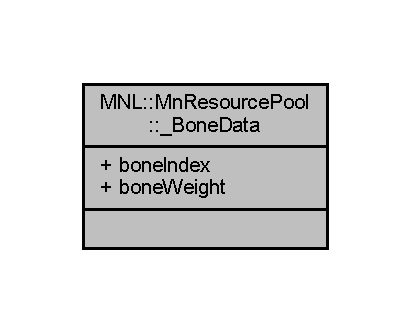
\includegraphics[width=197pt]{struct_m_n_l_1_1_mn_resource_pool_1_1___bone_data__coll__graph}
\end{center}
\end{figure}
\subsection*{Public 속성}
\begin{DoxyCompactItemize}
\item 
U\+I\+NT \hyperlink{struct_m_n_l_1_1_mn_resource_pool_1_1___bone_data_a9b932ff393564d1bed51b6a061e5bf7e}{bone\+Index} \mbox{[}4\mbox{]} = \{ 0, \}
\item 
float \hyperlink{struct_m_n_l_1_1_mn_resource_pool_1_1___bone_data_a95848ae147b2eca3bfdbcebde21441f6}{bone\+Weight} \mbox{[}4\mbox{]} = \{ 0.\+0f, \}
\end{DoxyCompactItemize}


\subsection{상세한 설명}


Mn\+Resource\+Pool.\+h 파일의 35 번째 라인에서 정의되었습니다.



\subsection{멤버 데이터 문서화}
\mbox{\Hypertarget{struct_m_n_l_1_1_mn_resource_pool_1_1___bone_data_a9b932ff393564d1bed51b6a061e5bf7e}\label{struct_m_n_l_1_1_mn_resource_pool_1_1___bone_data_a9b932ff393564d1bed51b6a061e5bf7e}} 
\index{M\+N\+L\+::\+Mn\+Resource\+Pool\+::\+\_\+\+Bone\+Data@{M\+N\+L\+::\+Mn\+Resource\+Pool\+::\+\_\+\+Bone\+Data}!bone\+Index@{bone\+Index}}
\index{bone\+Index@{bone\+Index}!M\+N\+L\+::\+Mn\+Resource\+Pool\+::\+\_\+\+Bone\+Data@{M\+N\+L\+::\+Mn\+Resource\+Pool\+::\+\_\+\+Bone\+Data}}
\subsubsection{\texorpdfstring{bone\+Index}{boneIndex}}
{\footnotesize\ttfamily U\+I\+NT M\+N\+L\+::\+Mn\+Resource\+Pool\+::\+\_\+\+Bone\+Data\+::bone\+Index\mbox{[}4\mbox{]} = \{ 0, \}}



Mn\+Resource\+Pool.\+h 파일의 37 번째 라인에서 정의되었습니다.

\mbox{\Hypertarget{struct_m_n_l_1_1_mn_resource_pool_1_1___bone_data_a95848ae147b2eca3bfdbcebde21441f6}\label{struct_m_n_l_1_1_mn_resource_pool_1_1___bone_data_a95848ae147b2eca3bfdbcebde21441f6}} 
\index{M\+N\+L\+::\+Mn\+Resource\+Pool\+::\+\_\+\+Bone\+Data@{M\+N\+L\+::\+Mn\+Resource\+Pool\+::\+\_\+\+Bone\+Data}!bone\+Weight@{bone\+Weight}}
\index{bone\+Weight@{bone\+Weight}!M\+N\+L\+::\+Mn\+Resource\+Pool\+::\+\_\+\+Bone\+Data@{M\+N\+L\+::\+Mn\+Resource\+Pool\+::\+\_\+\+Bone\+Data}}
\subsubsection{\texorpdfstring{bone\+Weight}{boneWeight}}
{\footnotesize\ttfamily float M\+N\+L\+::\+Mn\+Resource\+Pool\+::\+\_\+\+Bone\+Data\+::bone\+Weight\mbox{[}4\mbox{]} = \{ 0.\+0f, \}}



Mn\+Resource\+Pool.\+h 파일의 38 번째 라인에서 정의되었습니다.



이 구조체에 대한 문서화 페이지는 다음의 파일로부터 생성되었습니다.\+:\begin{DoxyCompactItemize}
\item 
Utility/\hyperlink{_mn_resource_pool_8h}{Mn\+Resource\+Pool.\+h}\end{DoxyCompactItemize}

\hypertarget{struct_m_n_l_1_1_mn_skinned_mesh_renderer_1_1___bone_palette_buffer_type}{}\section{M\+NL\+:\+:Mn\+Skinned\+Mesh\+Renderer\+:\+:\+\_\+\+Bone\+Palette\+Buffer\+Type 구조체 참조}
\label{struct_m_n_l_1_1_mn_skinned_mesh_renderer_1_1___bone_palette_buffer_type}\index{M\+N\+L\+::\+Mn\+Skinned\+Mesh\+Renderer\+::\+\_\+\+Bone\+Palette\+Buffer\+Type@{M\+N\+L\+::\+Mn\+Skinned\+Mesh\+Renderer\+::\+\_\+\+Bone\+Palette\+Buffer\+Type}}


M\+NL\+:\+:Mn\+Skinned\+Mesh\+Renderer\+:\+:\+\_\+\+Bone\+Palette\+Buffer\+Type에 대한 협력 다이어그램\+:\nopagebreak
\begin{figure}[H]
\begin{center}
\leavevmode
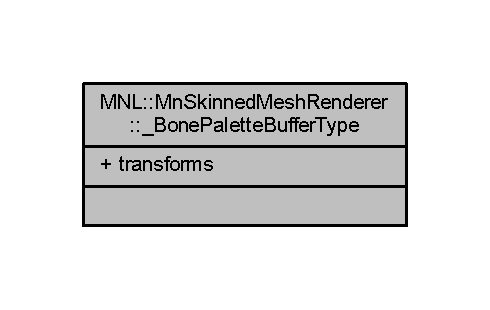
\includegraphics[width=235pt]{struct_m_n_l_1_1_mn_skinned_mesh_renderer_1_1___bone_palette_buffer_type__coll__graph}
\end{center}
\end{figure}
\subsection*{Public 속성}
\begin{DoxyCompactItemize}
\item 
Direct\+X\+::\+Simple\+Math\+::\+Matrix \hyperlink{struct_m_n_l_1_1_mn_skinned_mesh_renderer_1_1___bone_palette_buffer_type_a2b96ca83d6a5261a4dacaa4089704b22}{transforms} \mbox{[}96\mbox{]}
\end{DoxyCompactItemize}


\subsection{상세한 설명}


Mn\+Skinned\+Mesh\+Renderer.\+h 파일의 60 번째 라인에서 정의되었습니다.



\subsection{멤버 데이터 문서화}
\mbox{\Hypertarget{struct_m_n_l_1_1_mn_skinned_mesh_renderer_1_1___bone_palette_buffer_type_a2b96ca83d6a5261a4dacaa4089704b22}\label{struct_m_n_l_1_1_mn_skinned_mesh_renderer_1_1___bone_palette_buffer_type_a2b96ca83d6a5261a4dacaa4089704b22}} 
\index{M\+N\+L\+::\+Mn\+Skinned\+Mesh\+Renderer\+::\+\_\+\+Bone\+Palette\+Buffer\+Type@{M\+N\+L\+::\+Mn\+Skinned\+Mesh\+Renderer\+::\+\_\+\+Bone\+Palette\+Buffer\+Type}!transforms@{transforms}}
\index{transforms@{transforms}!M\+N\+L\+::\+Mn\+Skinned\+Mesh\+Renderer\+::\+\_\+\+Bone\+Palette\+Buffer\+Type@{M\+N\+L\+::\+Mn\+Skinned\+Mesh\+Renderer\+::\+\_\+\+Bone\+Palette\+Buffer\+Type}}
\subsubsection{\texorpdfstring{transforms}{transforms}}
{\footnotesize\ttfamily Direct\+X\+::\+Simple\+Math\+::\+Matrix M\+N\+L\+::\+Mn\+Skinned\+Mesh\+Renderer\+::\+\_\+\+Bone\+Palette\+Buffer\+Type\+::transforms\mbox{[}96\mbox{]}}



Mn\+Skinned\+Mesh\+Renderer.\+h 파일의 62 번째 라인에서 정의되었습니다.



이 구조체에 대한 문서화 페이지는 다음의 파일로부터 생성되었습니다.\+:\begin{DoxyCompactItemize}
\item 
Render/\hyperlink{_mn_skinned_mesh_renderer_8h}{Mn\+Skinned\+Mesh\+Renderer.\+h}\end{DoxyCompactItemize}

\hypertarget{struct_m_n_l_1_1_mn_mesh_renderer_1_1___light_buffer_type}{}\section{M\+NL\+:\+:Mn\+Mesh\+Renderer\+:\+:\+\_\+\+Light\+Buffer\+Type 구조체 참조}
\label{struct_m_n_l_1_1_mn_mesh_renderer_1_1___light_buffer_type}\index{M\+N\+L\+::\+Mn\+Mesh\+Renderer\+::\+\_\+\+Light\+Buffer\+Type@{M\+N\+L\+::\+Mn\+Mesh\+Renderer\+::\+\_\+\+Light\+Buffer\+Type}}


M\+NL\+:\+:Mn\+Mesh\+Renderer\+:\+:\+\_\+\+Light\+Buffer\+Type에 대한 협력 다이어그램\+:\nopagebreak
\begin{figure}[H]
\begin{center}
\leavevmode
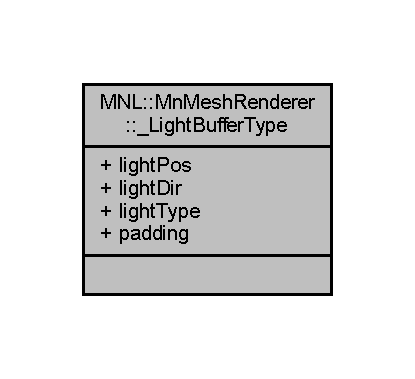
\includegraphics[width=199pt]{struct_m_n_l_1_1_mn_mesh_renderer_1_1___light_buffer_type__coll__graph}
\end{center}
\end{figure}
\subsection*{Public 속성}
\begin{DoxyCompactItemize}
\item 
Direct\+X\+::\+Simple\+Math\+::\+Vector4 \hyperlink{struct_m_n_l_1_1_mn_mesh_renderer_1_1___light_buffer_type_aab3a0d88cba1db5892f6b9a1000e8e04}{light\+Pos}
\item 
Direct\+X\+::\+Simple\+Math\+::\+Vector4 \hyperlink{struct_m_n_l_1_1_mn_mesh_renderer_1_1___light_buffer_type_a1e79199e1f7cd6c1bdbf06fdc1741fb3}{light\+Dir}
\item 
U\+I\+NT \hyperlink{struct_m_n_l_1_1_mn_mesh_renderer_1_1___light_buffer_type_ab945d609e87caa088353041ec308251f}{light\+Type}
\item 
Direct\+X\+::\+Simple\+Math\+::\+Vector3 \hyperlink{struct_m_n_l_1_1_mn_mesh_renderer_1_1___light_buffer_type_a5f16d547a936d5c03125973a11167d01}{padding}
\end{DoxyCompactItemize}


\subsection{상세한 설명}


Mn\+Mesh\+Renderer.\+h 파일의 39 번째 라인에서 정의되었습니다.



\subsection{멤버 데이터 문서화}
\mbox{\Hypertarget{struct_m_n_l_1_1_mn_mesh_renderer_1_1___light_buffer_type_a1e79199e1f7cd6c1bdbf06fdc1741fb3}\label{struct_m_n_l_1_1_mn_mesh_renderer_1_1___light_buffer_type_a1e79199e1f7cd6c1bdbf06fdc1741fb3}} 
\index{M\+N\+L\+::\+Mn\+Mesh\+Renderer\+::\+\_\+\+Light\+Buffer\+Type@{M\+N\+L\+::\+Mn\+Mesh\+Renderer\+::\+\_\+\+Light\+Buffer\+Type}!light\+Dir@{light\+Dir}}
\index{light\+Dir@{light\+Dir}!M\+N\+L\+::\+Mn\+Mesh\+Renderer\+::\+\_\+\+Light\+Buffer\+Type@{M\+N\+L\+::\+Mn\+Mesh\+Renderer\+::\+\_\+\+Light\+Buffer\+Type}}
\subsubsection{\texorpdfstring{light\+Dir}{lightDir}}
{\footnotesize\ttfamily Direct\+X\+::\+Simple\+Math\+::\+Vector4 M\+N\+L\+::\+Mn\+Mesh\+Renderer\+::\+\_\+\+Light\+Buffer\+Type\+::light\+Dir}



Mn\+Mesh\+Renderer.\+h 파일의 42 번째 라인에서 정의되었습니다.

\mbox{\Hypertarget{struct_m_n_l_1_1_mn_mesh_renderer_1_1___light_buffer_type_aab3a0d88cba1db5892f6b9a1000e8e04}\label{struct_m_n_l_1_1_mn_mesh_renderer_1_1___light_buffer_type_aab3a0d88cba1db5892f6b9a1000e8e04}} 
\index{M\+N\+L\+::\+Mn\+Mesh\+Renderer\+::\+\_\+\+Light\+Buffer\+Type@{M\+N\+L\+::\+Mn\+Mesh\+Renderer\+::\+\_\+\+Light\+Buffer\+Type}!light\+Pos@{light\+Pos}}
\index{light\+Pos@{light\+Pos}!M\+N\+L\+::\+Mn\+Mesh\+Renderer\+::\+\_\+\+Light\+Buffer\+Type@{M\+N\+L\+::\+Mn\+Mesh\+Renderer\+::\+\_\+\+Light\+Buffer\+Type}}
\subsubsection{\texorpdfstring{light\+Pos}{lightPos}}
{\footnotesize\ttfamily Direct\+X\+::\+Simple\+Math\+::\+Vector4 M\+N\+L\+::\+Mn\+Mesh\+Renderer\+::\+\_\+\+Light\+Buffer\+Type\+::light\+Pos}



Mn\+Mesh\+Renderer.\+h 파일의 41 번째 라인에서 정의되었습니다.

\mbox{\Hypertarget{struct_m_n_l_1_1_mn_mesh_renderer_1_1___light_buffer_type_ab945d609e87caa088353041ec308251f}\label{struct_m_n_l_1_1_mn_mesh_renderer_1_1___light_buffer_type_ab945d609e87caa088353041ec308251f}} 
\index{M\+N\+L\+::\+Mn\+Mesh\+Renderer\+::\+\_\+\+Light\+Buffer\+Type@{M\+N\+L\+::\+Mn\+Mesh\+Renderer\+::\+\_\+\+Light\+Buffer\+Type}!light\+Type@{light\+Type}}
\index{light\+Type@{light\+Type}!M\+N\+L\+::\+Mn\+Mesh\+Renderer\+::\+\_\+\+Light\+Buffer\+Type@{M\+N\+L\+::\+Mn\+Mesh\+Renderer\+::\+\_\+\+Light\+Buffer\+Type}}
\subsubsection{\texorpdfstring{light\+Type}{lightType}}
{\footnotesize\ttfamily U\+I\+NT M\+N\+L\+::\+Mn\+Mesh\+Renderer\+::\+\_\+\+Light\+Buffer\+Type\+::light\+Type}



Mn\+Mesh\+Renderer.\+h 파일의 43 번째 라인에서 정의되었습니다.

\mbox{\Hypertarget{struct_m_n_l_1_1_mn_mesh_renderer_1_1___light_buffer_type_a5f16d547a936d5c03125973a11167d01}\label{struct_m_n_l_1_1_mn_mesh_renderer_1_1___light_buffer_type_a5f16d547a936d5c03125973a11167d01}} 
\index{M\+N\+L\+::\+Mn\+Mesh\+Renderer\+::\+\_\+\+Light\+Buffer\+Type@{M\+N\+L\+::\+Mn\+Mesh\+Renderer\+::\+\_\+\+Light\+Buffer\+Type}!padding@{padding}}
\index{padding@{padding}!M\+N\+L\+::\+Mn\+Mesh\+Renderer\+::\+\_\+\+Light\+Buffer\+Type@{M\+N\+L\+::\+Mn\+Mesh\+Renderer\+::\+\_\+\+Light\+Buffer\+Type}}
\subsubsection{\texorpdfstring{padding}{padding}}
{\footnotesize\ttfamily Direct\+X\+::\+Simple\+Math\+::\+Vector3 M\+N\+L\+::\+Mn\+Mesh\+Renderer\+::\+\_\+\+Light\+Buffer\+Type\+::padding}



Mn\+Mesh\+Renderer.\+h 파일의 44 번째 라인에서 정의되었습니다.



이 구조체에 대한 문서화 페이지는 다음의 파일로부터 생성되었습니다.\+:\begin{DoxyCompactItemize}
\item 
Render/\hyperlink{_mn_mesh_renderer_8h}{Mn\+Mesh\+Renderer.\+h}\end{DoxyCompactItemize}

\hypertarget{struct_m_n_l_1_1_mn_skinned_mesh_renderer_1_1___light_buffer_type}{}\section{M\+NL\+:\+:Mn\+Skinned\+Mesh\+Renderer\+:\+:\+\_\+\+Light\+Buffer\+Type 구조체 참조}
\label{struct_m_n_l_1_1_mn_skinned_mesh_renderer_1_1___light_buffer_type}\index{M\+N\+L\+::\+Mn\+Skinned\+Mesh\+Renderer\+::\+\_\+\+Light\+Buffer\+Type@{M\+N\+L\+::\+Mn\+Skinned\+Mesh\+Renderer\+::\+\_\+\+Light\+Buffer\+Type}}


M\+NL\+:\+:Mn\+Skinned\+Mesh\+Renderer\+:\+:\+\_\+\+Light\+Buffer\+Type에 대한 협력 다이어그램\+:\nopagebreak
\begin{figure}[H]
\begin{center}
\leavevmode
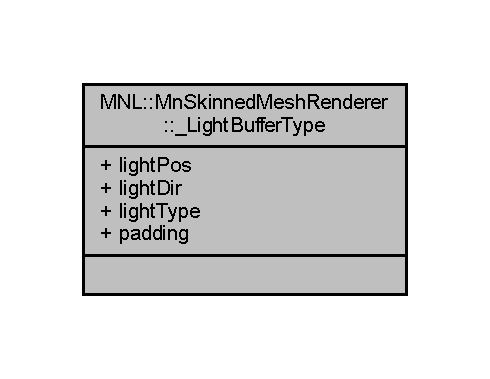
\includegraphics[width=235pt]{struct_m_n_l_1_1_mn_skinned_mesh_renderer_1_1___light_buffer_type__coll__graph}
\end{center}
\end{figure}
\subsection*{Public 속성}
\begin{DoxyCompactItemize}
\item 
Direct\+X\+::\+Simple\+Math\+::\+Vector4 \hyperlink{struct_m_n_l_1_1_mn_skinned_mesh_renderer_1_1___light_buffer_type_a3b2648fb7a53ce9be3c70dde56a2a7e6}{light\+Pos}
\item 
Direct\+X\+::\+Simple\+Math\+::\+Vector4 \hyperlink{struct_m_n_l_1_1_mn_skinned_mesh_renderer_1_1___light_buffer_type_ab0db31c912e02314a132688390771913}{light\+Dir}
\item 
U\+I\+NT \hyperlink{struct_m_n_l_1_1_mn_skinned_mesh_renderer_1_1___light_buffer_type_a6719a54f505e7a34b0f74a01973db0d0}{light\+Type}
\item 
Direct\+X\+::\+Simple\+Math\+::\+Vector3 \hyperlink{struct_m_n_l_1_1_mn_skinned_mesh_renderer_1_1___light_buffer_type_a6f2c2a324da4a7f48f3538f504a42e47}{padding}
\end{DoxyCompactItemize}


\subsection{상세한 설명}


Mn\+Skinned\+Mesh\+Renderer.\+h 파일의 41 번째 라인에서 정의되었습니다.



\subsection{멤버 데이터 문서화}
\mbox{\Hypertarget{struct_m_n_l_1_1_mn_skinned_mesh_renderer_1_1___light_buffer_type_ab0db31c912e02314a132688390771913}\label{struct_m_n_l_1_1_mn_skinned_mesh_renderer_1_1___light_buffer_type_ab0db31c912e02314a132688390771913}} 
\index{M\+N\+L\+::\+Mn\+Skinned\+Mesh\+Renderer\+::\+\_\+\+Light\+Buffer\+Type@{M\+N\+L\+::\+Mn\+Skinned\+Mesh\+Renderer\+::\+\_\+\+Light\+Buffer\+Type}!light\+Dir@{light\+Dir}}
\index{light\+Dir@{light\+Dir}!M\+N\+L\+::\+Mn\+Skinned\+Mesh\+Renderer\+::\+\_\+\+Light\+Buffer\+Type@{M\+N\+L\+::\+Mn\+Skinned\+Mesh\+Renderer\+::\+\_\+\+Light\+Buffer\+Type}}
\subsubsection{\texorpdfstring{light\+Dir}{lightDir}}
{\footnotesize\ttfamily Direct\+X\+::\+Simple\+Math\+::\+Vector4 M\+N\+L\+::\+Mn\+Skinned\+Mesh\+Renderer\+::\+\_\+\+Light\+Buffer\+Type\+::light\+Dir}



Mn\+Skinned\+Mesh\+Renderer.\+h 파일의 44 번째 라인에서 정의되었습니다.

\mbox{\Hypertarget{struct_m_n_l_1_1_mn_skinned_mesh_renderer_1_1___light_buffer_type_a3b2648fb7a53ce9be3c70dde56a2a7e6}\label{struct_m_n_l_1_1_mn_skinned_mesh_renderer_1_1___light_buffer_type_a3b2648fb7a53ce9be3c70dde56a2a7e6}} 
\index{M\+N\+L\+::\+Mn\+Skinned\+Mesh\+Renderer\+::\+\_\+\+Light\+Buffer\+Type@{M\+N\+L\+::\+Mn\+Skinned\+Mesh\+Renderer\+::\+\_\+\+Light\+Buffer\+Type}!light\+Pos@{light\+Pos}}
\index{light\+Pos@{light\+Pos}!M\+N\+L\+::\+Mn\+Skinned\+Mesh\+Renderer\+::\+\_\+\+Light\+Buffer\+Type@{M\+N\+L\+::\+Mn\+Skinned\+Mesh\+Renderer\+::\+\_\+\+Light\+Buffer\+Type}}
\subsubsection{\texorpdfstring{light\+Pos}{lightPos}}
{\footnotesize\ttfamily Direct\+X\+::\+Simple\+Math\+::\+Vector4 M\+N\+L\+::\+Mn\+Skinned\+Mesh\+Renderer\+::\+\_\+\+Light\+Buffer\+Type\+::light\+Pos}



Mn\+Skinned\+Mesh\+Renderer.\+h 파일의 43 번째 라인에서 정의되었습니다.

\mbox{\Hypertarget{struct_m_n_l_1_1_mn_skinned_mesh_renderer_1_1___light_buffer_type_a6719a54f505e7a34b0f74a01973db0d0}\label{struct_m_n_l_1_1_mn_skinned_mesh_renderer_1_1___light_buffer_type_a6719a54f505e7a34b0f74a01973db0d0}} 
\index{M\+N\+L\+::\+Mn\+Skinned\+Mesh\+Renderer\+::\+\_\+\+Light\+Buffer\+Type@{M\+N\+L\+::\+Mn\+Skinned\+Mesh\+Renderer\+::\+\_\+\+Light\+Buffer\+Type}!light\+Type@{light\+Type}}
\index{light\+Type@{light\+Type}!M\+N\+L\+::\+Mn\+Skinned\+Mesh\+Renderer\+::\+\_\+\+Light\+Buffer\+Type@{M\+N\+L\+::\+Mn\+Skinned\+Mesh\+Renderer\+::\+\_\+\+Light\+Buffer\+Type}}
\subsubsection{\texorpdfstring{light\+Type}{lightType}}
{\footnotesize\ttfamily U\+I\+NT M\+N\+L\+::\+Mn\+Skinned\+Mesh\+Renderer\+::\+\_\+\+Light\+Buffer\+Type\+::light\+Type}



Mn\+Skinned\+Mesh\+Renderer.\+h 파일의 45 번째 라인에서 정의되었습니다.

\mbox{\Hypertarget{struct_m_n_l_1_1_mn_skinned_mesh_renderer_1_1___light_buffer_type_a6f2c2a324da4a7f48f3538f504a42e47}\label{struct_m_n_l_1_1_mn_skinned_mesh_renderer_1_1___light_buffer_type_a6f2c2a324da4a7f48f3538f504a42e47}} 
\index{M\+N\+L\+::\+Mn\+Skinned\+Mesh\+Renderer\+::\+\_\+\+Light\+Buffer\+Type@{M\+N\+L\+::\+Mn\+Skinned\+Mesh\+Renderer\+::\+\_\+\+Light\+Buffer\+Type}!padding@{padding}}
\index{padding@{padding}!M\+N\+L\+::\+Mn\+Skinned\+Mesh\+Renderer\+::\+\_\+\+Light\+Buffer\+Type@{M\+N\+L\+::\+Mn\+Skinned\+Mesh\+Renderer\+::\+\_\+\+Light\+Buffer\+Type}}
\subsubsection{\texorpdfstring{padding}{padding}}
{\footnotesize\ttfamily Direct\+X\+::\+Simple\+Math\+::\+Vector3 M\+N\+L\+::\+Mn\+Skinned\+Mesh\+Renderer\+::\+\_\+\+Light\+Buffer\+Type\+::padding}



Mn\+Skinned\+Mesh\+Renderer.\+h 파일의 46 번째 라인에서 정의되었습니다.



이 구조체에 대한 문서화 페이지는 다음의 파일로부터 생성되었습니다.\+:\begin{DoxyCompactItemize}
\item 
Render/\hyperlink{_mn_skinned_mesh_renderer_8h}{Mn\+Skinned\+Mesh\+Renderer.\+h}\end{DoxyCompactItemize}

\hypertarget{struct_m_n_l_1_1_mn_mesh_renderer_1_1___material_buffer_type}{}\section{M\+NL\+:\+:Mn\+Mesh\+Renderer\+:\+:\+\_\+\+Material\+Buffer\+Type 구조체 참조}
\label{struct_m_n_l_1_1_mn_mesh_renderer_1_1___material_buffer_type}\index{M\+N\+L\+::\+Mn\+Mesh\+Renderer\+::\+\_\+\+Material\+Buffer\+Type@{M\+N\+L\+::\+Mn\+Mesh\+Renderer\+::\+\_\+\+Material\+Buffer\+Type}}


M\+NL\+:\+:Mn\+Mesh\+Renderer\+:\+:\+\_\+\+Material\+Buffer\+Type에 대한 협력 다이어그램\+:\nopagebreak
\begin{figure}[H]
\begin{center}
\leavevmode
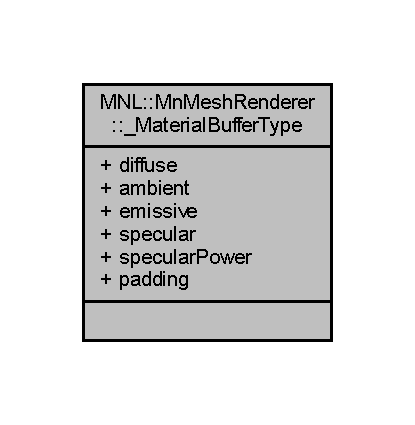
\includegraphics[width=199pt]{struct_m_n_l_1_1_mn_mesh_renderer_1_1___material_buffer_type__coll__graph}
\end{center}
\end{figure}
\subsection*{Public 속성}
\begin{DoxyCompactItemize}
\item 
Direct\+X\+::\+Simple\+Math\+::\+Vector4 \hyperlink{struct_m_n_l_1_1_mn_mesh_renderer_1_1___material_buffer_type_a7ff9130e983158bd74e7a5fb29d24b3e}{diffuse}
\item 
Direct\+X\+::\+Simple\+Math\+::\+Vector4 \hyperlink{struct_m_n_l_1_1_mn_mesh_renderer_1_1___material_buffer_type_aee327bbcf5e0c85bad6bc3a374f3a98c}{ambient}
\item 
Direct\+X\+::\+Simple\+Math\+::\+Vector4 \hyperlink{struct_m_n_l_1_1_mn_mesh_renderer_1_1___material_buffer_type_a5d2d43bd56e7d8aea2456632386fc8d4}{emissive}
\item 
Direct\+X\+::\+Simple\+Math\+::\+Vector4 \hyperlink{struct_m_n_l_1_1_mn_mesh_renderer_1_1___material_buffer_type_a7ae76ae36b475d3ef989862a8a9bc37a}{specular}
\item 
float \hyperlink{struct_m_n_l_1_1_mn_mesh_renderer_1_1___material_buffer_type_a6c5c3373b1f35531a3f0d7fd6afc819e}{specular\+Power}
\item 
Direct\+X\+::\+Simple\+Math\+::\+Vector3 \hyperlink{struct_m_n_l_1_1_mn_mesh_renderer_1_1___material_buffer_type_a9ca8141e828bb09ea15d1bd486535f41}{padding}
\end{DoxyCompactItemize}


\subsection{상세한 설명}


Mn\+Mesh\+Renderer.\+h 파일의 46 번째 라인에서 정의되었습니다.



\subsection{멤버 데이터 문서화}
\mbox{\Hypertarget{struct_m_n_l_1_1_mn_mesh_renderer_1_1___material_buffer_type_aee327bbcf5e0c85bad6bc3a374f3a98c}\label{struct_m_n_l_1_1_mn_mesh_renderer_1_1___material_buffer_type_aee327bbcf5e0c85bad6bc3a374f3a98c}} 
\index{M\+N\+L\+::\+Mn\+Mesh\+Renderer\+::\+\_\+\+Material\+Buffer\+Type@{M\+N\+L\+::\+Mn\+Mesh\+Renderer\+::\+\_\+\+Material\+Buffer\+Type}!ambient@{ambient}}
\index{ambient@{ambient}!M\+N\+L\+::\+Mn\+Mesh\+Renderer\+::\+\_\+\+Material\+Buffer\+Type@{M\+N\+L\+::\+Mn\+Mesh\+Renderer\+::\+\_\+\+Material\+Buffer\+Type}}
\subsubsection{\texorpdfstring{ambient}{ambient}}
{\footnotesize\ttfamily Direct\+X\+::\+Simple\+Math\+::\+Vector4 M\+N\+L\+::\+Mn\+Mesh\+Renderer\+::\+\_\+\+Material\+Buffer\+Type\+::ambient}



Mn\+Mesh\+Renderer.\+h 파일의 49 번째 라인에서 정의되었습니다.

\mbox{\Hypertarget{struct_m_n_l_1_1_mn_mesh_renderer_1_1___material_buffer_type_a7ff9130e983158bd74e7a5fb29d24b3e}\label{struct_m_n_l_1_1_mn_mesh_renderer_1_1___material_buffer_type_a7ff9130e983158bd74e7a5fb29d24b3e}} 
\index{M\+N\+L\+::\+Mn\+Mesh\+Renderer\+::\+\_\+\+Material\+Buffer\+Type@{M\+N\+L\+::\+Mn\+Mesh\+Renderer\+::\+\_\+\+Material\+Buffer\+Type}!diffuse@{diffuse}}
\index{diffuse@{diffuse}!M\+N\+L\+::\+Mn\+Mesh\+Renderer\+::\+\_\+\+Material\+Buffer\+Type@{M\+N\+L\+::\+Mn\+Mesh\+Renderer\+::\+\_\+\+Material\+Buffer\+Type}}
\subsubsection{\texorpdfstring{diffuse}{diffuse}}
{\footnotesize\ttfamily Direct\+X\+::\+Simple\+Math\+::\+Vector4 M\+N\+L\+::\+Mn\+Mesh\+Renderer\+::\+\_\+\+Material\+Buffer\+Type\+::diffuse}



Mn\+Mesh\+Renderer.\+h 파일의 48 번째 라인에서 정의되었습니다.

\mbox{\Hypertarget{struct_m_n_l_1_1_mn_mesh_renderer_1_1___material_buffer_type_a5d2d43bd56e7d8aea2456632386fc8d4}\label{struct_m_n_l_1_1_mn_mesh_renderer_1_1___material_buffer_type_a5d2d43bd56e7d8aea2456632386fc8d4}} 
\index{M\+N\+L\+::\+Mn\+Mesh\+Renderer\+::\+\_\+\+Material\+Buffer\+Type@{M\+N\+L\+::\+Mn\+Mesh\+Renderer\+::\+\_\+\+Material\+Buffer\+Type}!emissive@{emissive}}
\index{emissive@{emissive}!M\+N\+L\+::\+Mn\+Mesh\+Renderer\+::\+\_\+\+Material\+Buffer\+Type@{M\+N\+L\+::\+Mn\+Mesh\+Renderer\+::\+\_\+\+Material\+Buffer\+Type}}
\subsubsection{\texorpdfstring{emissive}{emissive}}
{\footnotesize\ttfamily Direct\+X\+::\+Simple\+Math\+::\+Vector4 M\+N\+L\+::\+Mn\+Mesh\+Renderer\+::\+\_\+\+Material\+Buffer\+Type\+::emissive}



Mn\+Mesh\+Renderer.\+h 파일의 50 번째 라인에서 정의되었습니다.

\mbox{\Hypertarget{struct_m_n_l_1_1_mn_mesh_renderer_1_1___material_buffer_type_a9ca8141e828bb09ea15d1bd486535f41}\label{struct_m_n_l_1_1_mn_mesh_renderer_1_1___material_buffer_type_a9ca8141e828bb09ea15d1bd486535f41}} 
\index{M\+N\+L\+::\+Mn\+Mesh\+Renderer\+::\+\_\+\+Material\+Buffer\+Type@{M\+N\+L\+::\+Mn\+Mesh\+Renderer\+::\+\_\+\+Material\+Buffer\+Type}!padding@{padding}}
\index{padding@{padding}!M\+N\+L\+::\+Mn\+Mesh\+Renderer\+::\+\_\+\+Material\+Buffer\+Type@{M\+N\+L\+::\+Mn\+Mesh\+Renderer\+::\+\_\+\+Material\+Buffer\+Type}}
\subsubsection{\texorpdfstring{padding}{padding}}
{\footnotesize\ttfamily Direct\+X\+::\+Simple\+Math\+::\+Vector3 M\+N\+L\+::\+Mn\+Mesh\+Renderer\+::\+\_\+\+Material\+Buffer\+Type\+::padding}



Mn\+Mesh\+Renderer.\+h 파일의 53 번째 라인에서 정의되었습니다.

\mbox{\Hypertarget{struct_m_n_l_1_1_mn_mesh_renderer_1_1___material_buffer_type_a7ae76ae36b475d3ef989862a8a9bc37a}\label{struct_m_n_l_1_1_mn_mesh_renderer_1_1___material_buffer_type_a7ae76ae36b475d3ef989862a8a9bc37a}} 
\index{M\+N\+L\+::\+Mn\+Mesh\+Renderer\+::\+\_\+\+Material\+Buffer\+Type@{M\+N\+L\+::\+Mn\+Mesh\+Renderer\+::\+\_\+\+Material\+Buffer\+Type}!specular@{specular}}
\index{specular@{specular}!M\+N\+L\+::\+Mn\+Mesh\+Renderer\+::\+\_\+\+Material\+Buffer\+Type@{M\+N\+L\+::\+Mn\+Mesh\+Renderer\+::\+\_\+\+Material\+Buffer\+Type}}
\subsubsection{\texorpdfstring{specular}{specular}}
{\footnotesize\ttfamily Direct\+X\+::\+Simple\+Math\+::\+Vector4 M\+N\+L\+::\+Mn\+Mesh\+Renderer\+::\+\_\+\+Material\+Buffer\+Type\+::specular}



Mn\+Mesh\+Renderer.\+h 파일의 51 번째 라인에서 정의되었습니다.

\mbox{\Hypertarget{struct_m_n_l_1_1_mn_mesh_renderer_1_1___material_buffer_type_a6c5c3373b1f35531a3f0d7fd6afc819e}\label{struct_m_n_l_1_1_mn_mesh_renderer_1_1___material_buffer_type_a6c5c3373b1f35531a3f0d7fd6afc819e}} 
\index{M\+N\+L\+::\+Mn\+Mesh\+Renderer\+::\+\_\+\+Material\+Buffer\+Type@{M\+N\+L\+::\+Mn\+Mesh\+Renderer\+::\+\_\+\+Material\+Buffer\+Type}!specular\+Power@{specular\+Power}}
\index{specular\+Power@{specular\+Power}!M\+N\+L\+::\+Mn\+Mesh\+Renderer\+::\+\_\+\+Material\+Buffer\+Type@{M\+N\+L\+::\+Mn\+Mesh\+Renderer\+::\+\_\+\+Material\+Buffer\+Type}}
\subsubsection{\texorpdfstring{specular\+Power}{specularPower}}
{\footnotesize\ttfamily float M\+N\+L\+::\+Mn\+Mesh\+Renderer\+::\+\_\+\+Material\+Buffer\+Type\+::specular\+Power}



Mn\+Mesh\+Renderer.\+h 파일의 52 번째 라인에서 정의되었습니다.



이 구조체에 대한 문서화 페이지는 다음의 파일로부터 생성되었습니다.\+:\begin{DoxyCompactItemize}
\item 
Render/\hyperlink{_mn_mesh_renderer_8h}{Mn\+Mesh\+Renderer.\+h}\end{DoxyCompactItemize}

\hypertarget{struct_m_n_l_1_1_mn_skinned_mesh_renderer_1_1___material_buffer_type}{}\section{M\+NL\+:\+:Mn\+Skinned\+Mesh\+Renderer\+:\+:\+\_\+\+Material\+Buffer\+Type 구조체 참조}
\label{struct_m_n_l_1_1_mn_skinned_mesh_renderer_1_1___material_buffer_type}\index{M\+N\+L\+::\+Mn\+Skinned\+Mesh\+Renderer\+::\+\_\+\+Material\+Buffer\+Type@{M\+N\+L\+::\+Mn\+Skinned\+Mesh\+Renderer\+::\+\_\+\+Material\+Buffer\+Type}}


M\+NL\+:\+:Mn\+Skinned\+Mesh\+Renderer\+:\+:\+\_\+\+Material\+Buffer\+Type에 대한 협력 다이어그램\+:\nopagebreak
\begin{figure}[H]
\begin{center}
\leavevmode
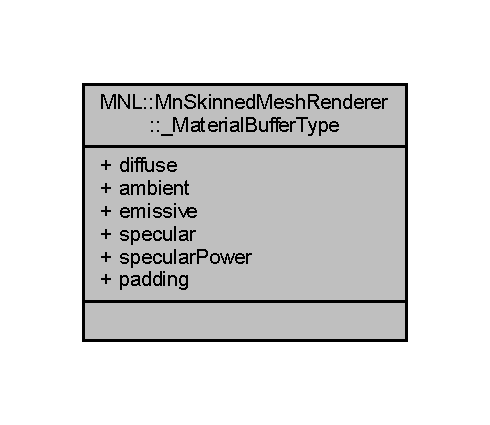
\includegraphics[width=235pt]{struct_m_n_l_1_1_mn_skinned_mesh_renderer_1_1___material_buffer_type__coll__graph}
\end{center}
\end{figure}
\subsection*{Public 속성}
\begin{DoxyCompactItemize}
\item 
Direct\+X\+::\+Simple\+Math\+::\+Vector4 \hyperlink{struct_m_n_l_1_1_mn_skinned_mesh_renderer_1_1___material_buffer_type_a8914fb757cebc4cf514a3123791c87a8}{diffuse}
\item 
Direct\+X\+::\+Simple\+Math\+::\+Vector4 \hyperlink{struct_m_n_l_1_1_mn_skinned_mesh_renderer_1_1___material_buffer_type_a81ae4e3c1f9fed177e8ca033ba5fad2a}{ambient}
\item 
Direct\+X\+::\+Simple\+Math\+::\+Vector4 \hyperlink{struct_m_n_l_1_1_mn_skinned_mesh_renderer_1_1___material_buffer_type_a5efa524269d7a25ff9dc59152156c5b2}{emissive}
\item 
Direct\+X\+::\+Simple\+Math\+::\+Vector4 \hyperlink{struct_m_n_l_1_1_mn_skinned_mesh_renderer_1_1___material_buffer_type_ae4a229660dfd6408e16f0b80e147aefe}{specular}
\item 
float \hyperlink{struct_m_n_l_1_1_mn_skinned_mesh_renderer_1_1___material_buffer_type_adf39c878cd0b12017cd7b1bf3afbdfe2}{specular\+Power}
\item 
Direct\+X\+::\+Simple\+Math\+::\+Vector3 \hyperlink{struct_m_n_l_1_1_mn_skinned_mesh_renderer_1_1___material_buffer_type_a1a083f0554c6ae75fd5b049f98f3f27b}{padding}
\end{DoxyCompactItemize}


\subsection{상세한 설명}


Mn\+Skinned\+Mesh\+Renderer.\+h 파일의 48 번째 라인에서 정의되었습니다.



\subsection{멤버 데이터 문서화}
\mbox{\Hypertarget{struct_m_n_l_1_1_mn_skinned_mesh_renderer_1_1___material_buffer_type_a81ae4e3c1f9fed177e8ca033ba5fad2a}\label{struct_m_n_l_1_1_mn_skinned_mesh_renderer_1_1___material_buffer_type_a81ae4e3c1f9fed177e8ca033ba5fad2a}} 
\index{M\+N\+L\+::\+Mn\+Skinned\+Mesh\+Renderer\+::\+\_\+\+Material\+Buffer\+Type@{M\+N\+L\+::\+Mn\+Skinned\+Mesh\+Renderer\+::\+\_\+\+Material\+Buffer\+Type}!ambient@{ambient}}
\index{ambient@{ambient}!M\+N\+L\+::\+Mn\+Skinned\+Mesh\+Renderer\+::\+\_\+\+Material\+Buffer\+Type@{M\+N\+L\+::\+Mn\+Skinned\+Mesh\+Renderer\+::\+\_\+\+Material\+Buffer\+Type}}
\subsubsection{\texorpdfstring{ambient}{ambient}}
{\footnotesize\ttfamily Direct\+X\+::\+Simple\+Math\+::\+Vector4 M\+N\+L\+::\+Mn\+Skinned\+Mesh\+Renderer\+::\+\_\+\+Material\+Buffer\+Type\+::ambient}



Mn\+Skinned\+Mesh\+Renderer.\+h 파일의 51 번째 라인에서 정의되었습니다.

\mbox{\Hypertarget{struct_m_n_l_1_1_mn_skinned_mesh_renderer_1_1___material_buffer_type_a8914fb757cebc4cf514a3123791c87a8}\label{struct_m_n_l_1_1_mn_skinned_mesh_renderer_1_1___material_buffer_type_a8914fb757cebc4cf514a3123791c87a8}} 
\index{M\+N\+L\+::\+Mn\+Skinned\+Mesh\+Renderer\+::\+\_\+\+Material\+Buffer\+Type@{M\+N\+L\+::\+Mn\+Skinned\+Mesh\+Renderer\+::\+\_\+\+Material\+Buffer\+Type}!diffuse@{diffuse}}
\index{diffuse@{diffuse}!M\+N\+L\+::\+Mn\+Skinned\+Mesh\+Renderer\+::\+\_\+\+Material\+Buffer\+Type@{M\+N\+L\+::\+Mn\+Skinned\+Mesh\+Renderer\+::\+\_\+\+Material\+Buffer\+Type}}
\subsubsection{\texorpdfstring{diffuse}{diffuse}}
{\footnotesize\ttfamily Direct\+X\+::\+Simple\+Math\+::\+Vector4 M\+N\+L\+::\+Mn\+Skinned\+Mesh\+Renderer\+::\+\_\+\+Material\+Buffer\+Type\+::diffuse}



Mn\+Skinned\+Mesh\+Renderer.\+h 파일의 50 번째 라인에서 정의되었습니다.

\mbox{\Hypertarget{struct_m_n_l_1_1_mn_skinned_mesh_renderer_1_1___material_buffer_type_a5efa524269d7a25ff9dc59152156c5b2}\label{struct_m_n_l_1_1_mn_skinned_mesh_renderer_1_1___material_buffer_type_a5efa524269d7a25ff9dc59152156c5b2}} 
\index{M\+N\+L\+::\+Mn\+Skinned\+Mesh\+Renderer\+::\+\_\+\+Material\+Buffer\+Type@{M\+N\+L\+::\+Mn\+Skinned\+Mesh\+Renderer\+::\+\_\+\+Material\+Buffer\+Type}!emissive@{emissive}}
\index{emissive@{emissive}!M\+N\+L\+::\+Mn\+Skinned\+Mesh\+Renderer\+::\+\_\+\+Material\+Buffer\+Type@{M\+N\+L\+::\+Mn\+Skinned\+Mesh\+Renderer\+::\+\_\+\+Material\+Buffer\+Type}}
\subsubsection{\texorpdfstring{emissive}{emissive}}
{\footnotesize\ttfamily Direct\+X\+::\+Simple\+Math\+::\+Vector4 M\+N\+L\+::\+Mn\+Skinned\+Mesh\+Renderer\+::\+\_\+\+Material\+Buffer\+Type\+::emissive}



Mn\+Skinned\+Mesh\+Renderer.\+h 파일의 52 번째 라인에서 정의되었습니다.

\mbox{\Hypertarget{struct_m_n_l_1_1_mn_skinned_mesh_renderer_1_1___material_buffer_type_a1a083f0554c6ae75fd5b049f98f3f27b}\label{struct_m_n_l_1_1_mn_skinned_mesh_renderer_1_1___material_buffer_type_a1a083f0554c6ae75fd5b049f98f3f27b}} 
\index{M\+N\+L\+::\+Mn\+Skinned\+Mesh\+Renderer\+::\+\_\+\+Material\+Buffer\+Type@{M\+N\+L\+::\+Mn\+Skinned\+Mesh\+Renderer\+::\+\_\+\+Material\+Buffer\+Type}!padding@{padding}}
\index{padding@{padding}!M\+N\+L\+::\+Mn\+Skinned\+Mesh\+Renderer\+::\+\_\+\+Material\+Buffer\+Type@{M\+N\+L\+::\+Mn\+Skinned\+Mesh\+Renderer\+::\+\_\+\+Material\+Buffer\+Type}}
\subsubsection{\texorpdfstring{padding}{padding}}
{\footnotesize\ttfamily Direct\+X\+::\+Simple\+Math\+::\+Vector3 M\+N\+L\+::\+Mn\+Skinned\+Mesh\+Renderer\+::\+\_\+\+Material\+Buffer\+Type\+::padding}



Mn\+Skinned\+Mesh\+Renderer.\+h 파일의 55 번째 라인에서 정의되었습니다.

\mbox{\Hypertarget{struct_m_n_l_1_1_mn_skinned_mesh_renderer_1_1___material_buffer_type_ae4a229660dfd6408e16f0b80e147aefe}\label{struct_m_n_l_1_1_mn_skinned_mesh_renderer_1_1___material_buffer_type_ae4a229660dfd6408e16f0b80e147aefe}} 
\index{M\+N\+L\+::\+Mn\+Skinned\+Mesh\+Renderer\+::\+\_\+\+Material\+Buffer\+Type@{M\+N\+L\+::\+Mn\+Skinned\+Mesh\+Renderer\+::\+\_\+\+Material\+Buffer\+Type}!specular@{specular}}
\index{specular@{specular}!M\+N\+L\+::\+Mn\+Skinned\+Mesh\+Renderer\+::\+\_\+\+Material\+Buffer\+Type@{M\+N\+L\+::\+Mn\+Skinned\+Mesh\+Renderer\+::\+\_\+\+Material\+Buffer\+Type}}
\subsubsection{\texorpdfstring{specular}{specular}}
{\footnotesize\ttfamily Direct\+X\+::\+Simple\+Math\+::\+Vector4 M\+N\+L\+::\+Mn\+Skinned\+Mesh\+Renderer\+::\+\_\+\+Material\+Buffer\+Type\+::specular}



Mn\+Skinned\+Mesh\+Renderer.\+h 파일의 53 번째 라인에서 정의되었습니다.

\mbox{\Hypertarget{struct_m_n_l_1_1_mn_skinned_mesh_renderer_1_1___material_buffer_type_adf39c878cd0b12017cd7b1bf3afbdfe2}\label{struct_m_n_l_1_1_mn_skinned_mesh_renderer_1_1___material_buffer_type_adf39c878cd0b12017cd7b1bf3afbdfe2}} 
\index{M\+N\+L\+::\+Mn\+Skinned\+Mesh\+Renderer\+::\+\_\+\+Material\+Buffer\+Type@{M\+N\+L\+::\+Mn\+Skinned\+Mesh\+Renderer\+::\+\_\+\+Material\+Buffer\+Type}!specular\+Power@{specular\+Power}}
\index{specular\+Power@{specular\+Power}!M\+N\+L\+::\+Mn\+Skinned\+Mesh\+Renderer\+::\+\_\+\+Material\+Buffer\+Type@{M\+N\+L\+::\+Mn\+Skinned\+Mesh\+Renderer\+::\+\_\+\+Material\+Buffer\+Type}}
\subsubsection{\texorpdfstring{specular\+Power}{specularPower}}
{\footnotesize\ttfamily float M\+N\+L\+::\+Mn\+Skinned\+Mesh\+Renderer\+::\+\_\+\+Material\+Buffer\+Type\+::specular\+Power}



Mn\+Skinned\+Mesh\+Renderer.\+h 파일의 54 번째 라인에서 정의되었습니다.



이 구조체에 대한 문서화 페이지는 다음의 파일로부터 생성되었습니다.\+:\begin{DoxyCompactItemize}
\item 
Render/\hyperlink{_mn_skinned_mesh_renderer_8h}{Mn\+Skinned\+Mesh\+Renderer.\+h}\end{DoxyCompactItemize}

\hypertarget{struct_m_n_l_1_1_mn_resource_pool_1_1___memory_chunk}{}\section{M\+NL\+:\+:Mn\+Resource\+Pool\+:\+:\+\_\+\+Memory\+Chunk 구조체 참조}
\label{struct_m_n_l_1_1_mn_resource_pool_1_1___memory_chunk}\index{M\+N\+L\+::\+Mn\+Resource\+Pool\+::\+\_\+\+Memory\+Chunk@{M\+N\+L\+::\+Mn\+Resource\+Pool\+::\+\_\+\+Memory\+Chunk}}


M\+NL\+:\+:Mn\+Resource\+Pool\+:\+:\+\_\+\+Memory\+Chunk에 대한 협력 다이어그램\+:\nopagebreak
\begin{figure}[H]
\begin{center}
\leavevmode
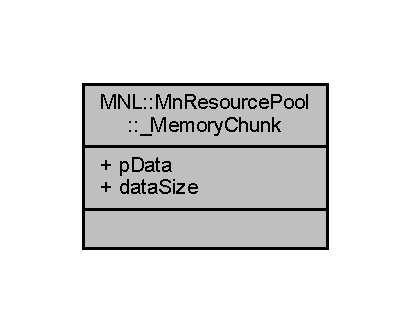
\includegraphics[width=197pt]{struct_m_n_l_1_1_mn_resource_pool_1_1___memory_chunk__coll__graph}
\end{center}
\end{figure}
\subsection*{Public 속성}
\begin{DoxyCompactItemize}
\item 
std\+::unique\+\_\+ptr$<$ char $>$ \hyperlink{struct_m_n_l_1_1_mn_resource_pool_1_1___memory_chunk_ad2b4ab69a299789920cd165e1a6c7196}{p\+Data}
\item 
U\+I\+NT \hyperlink{struct_m_n_l_1_1_mn_resource_pool_1_1___memory_chunk_a802a418104a49d2cb3a865d329cd1175}{data\+Size}
\end{DoxyCompactItemize}


\subsection{상세한 설명}


Mn\+Resource\+Pool.\+h 파일의 20 번째 라인에서 정의되었습니다.



\subsection{멤버 데이터 문서화}
\mbox{\Hypertarget{struct_m_n_l_1_1_mn_resource_pool_1_1___memory_chunk_a802a418104a49d2cb3a865d329cd1175}\label{struct_m_n_l_1_1_mn_resource_pool_1_1___memory_chunk_a802a418104a49d2cb3a865d329cd1175}} 
\index{M\+N\+L\+::\+Mn\+Resource\+Pool\+::\+\_\+\+Memory\+Chunk@{M\+N\+L\+::\+Mn\+Resource\+Pool\+::\+\_\+\+Memory\+Chunk}!data\+Size@{data\+Size}}
\index{data\+Size@{data\+Size}!M\+N\+L\+::\+Mn\+Resource\+Pool\+::\+\_\+\+Memory\+Chunk@{M\+N\+L\+::\+Mn\+Resource\+Pool\+::\+\_\+\+Memory\+Chunk}}
\subsubsection{\texorpdfstring{data\+Size}{dataSize}}
{\footnotesize\ttfamily U\+I\+NT M\+N\+L\+::\+Mn\+Resource\+Pool\+::\+\_\+\+Memory\+Chunk\+::data\+Size}



Mn\+Resource\+Pool.\+h 파일의 23 번째 라인에서 정의되었습니다.

\mbox{\Hypertarget{struct_m_n_l_1_1_mn_resource_pool_1_1___memory_chunk_ad2b4ab69a299789920cd165e1a6c7196}\label{struct_m_n_l_1_1_mn_resource_pool_1_1___memory_chunk_ad2b4ab69a299789920cd165e1a6c7196}} 
\index{M\+N\+L\+::\+Mn\+Resource\+Pool\+::\+\_\+\+Memory\+Chunk@{M\+N\+L\+::\+Mn\+Resource\+Pool\+::\+\_\+\+Memory\+Chunk}!p\+Data@{p\+Data}}
\index{p\+Data@{p\+Data}!M\+N\+L\+::\+Mn\+Resource\+Pool\+::\+\_\+\+Memory\+Chunk@{M\+N\+L\+::\+Mn\+Resource\+Pool\+::\+\_\+\+Memory\+Chunk}}
\subsubsection{\texorpdfstring{p\+Data}{pData}}
{\footnotesize\ttfamily std\+::unique\+\_\+ptr$<$char$>$ M\+N\+L\+::\+Mn\+Resource\+Pool\+::\+\_\+\+Memory\+Chunk\+::p\+Data}



Mn\+Resource\+Pool.\+h 파일의 22 번째 라인에서 정의되었습니다.



이 구조체에 대한 문서화 페이지는 다음의 파일로부터 생성되었습니다.\+:\begin{DoxyCompactItemize}
\item 
Utility/\hyperlink{_mn_resource_pool_8h}{Mn\+Resource\+Pool.\+h}\end{DoxyCompactItemize}

\hypertarget{struct_m_n_l_1_1_mn_resource_pool_1_1___model_package}{}\section{M\+NL\+:\+:Mn\+Resource\+Pool\+:\+:\+\_\+\+Model\+Package 구조체 참조}
\label{struct_m_n_l_1_1_mn_resource_pool_1_1___model_package}\index{M\+N\+L\+::\+Mn\+Resource\+Pool\+::\+\_\+\+Model\+Package@{M\+N\+L\+::\+Mn\+Resource\+Pool\+::\+\_\+\+Model\+Package}}


M\+NL\+:\+:Mn\+Resource\+Pool\+:\+:\+\_\+\+Model\+Package에 대한 협력 다이어그램\+:\nopagebreak
\begin{figure}[H]
\begin{center}
\leavevmode
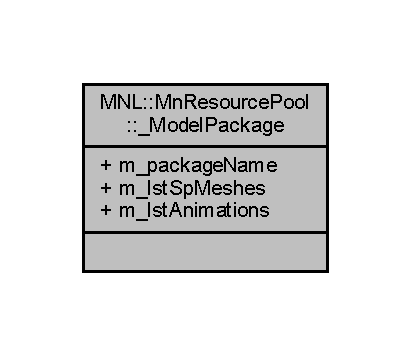
\includegraphics[width=197pt]{struct_m_n_l_1_1_mn_resource_pool_1_1___model_package__coll__graph}
\end{center}
\end{figure}
\subsection*{Public 속성}
\begin{DoxyCompactItemize}
\item 
std\+::string \hyperlink{struct_m_n_l_1_1_mn_resource_pool_1_1___model_package_ae206cfd79820ffa3e4d30169b977a068}{m\+\_\+package\+Name}
\item 
std\+::vector$<$ std\+::shared\+\_\+ptr$<$ \hyperlink{class_m_n_l_1_1_mn_mesh_data}{Mn\+Mesh\+Data} $>$ $>$ \hyperlink{struct_m_n_l_1_1_mn_resource_pool_1_1___model_package_a6ce290b16db878c61570750b1135dd7f}{m\+\_\+lst\+Sp\+Meshes}
\item 
std\+::vector$<$ \hyperlink{class_m_n_l_1_1_mn_bone_animation}{Mn\+Bone\+Animation} $>$ \hyperlink{struct_m_n_l_1_1_mn_resource_pool_1_1___model_package_a6e22d7d1c02f3c8700ccd6aa89264624}{m\+\_\+lst\+Animations}
\end{DoxyCompactItemize}


\subsection{상세한 설명}


Mn\+Resource\+Pool.\+h 파일의 28 번째 라인에서 정의되었습니다.



\subsection{멤버 데이터 문서화}
\mbox{\Hypertarget{struct_m_n_l_1_1_mn_resource_pool_1_1___model_package_a6e22d7d1c02f3c8700ccd6aa89264624}\label{struct_m_n_l_1_1_mn_resource_pool_1_1___model_package_a6e22d7d1c02f3c8700ccd6aa89264624}} 
\index{M\+N\+L\+::\+Mn\+Resource\+Pool\+::\+\_\+\+Model\+Package@{M\+N\+L\+::\+Mn\+Resource\+Pool\+::\+\_\+\+Model\+Package}!m\+\_\+lst\+Animations@{m\+\_\+lst\+Animations}}
\index{m\+\_\+lst\+Animations@{m\+\_\+lst\+Animations}!M\+N\+L\+::\+Mn\+Resource\+Pool\+::\+\_\+\+Model\+Package@{M\+N\+L\+::\+Mn\+Resource\+Pool\+::\+\_\+\+Model\+Package}}
\subsubsection{\texorpdfstring{m\+\_\+lst\+Animations}{m\_lstAnimations}}
{\footnotesize\ttfamily std\+::vector$<$\hyperlink{class_m_n_l_1_1_mn_bone_animation}{Mn\+Bone\+Animation}$>$ M\+N\+L\+::\+Mn\+Resource\+Pool\+::\+\_\+\+Model\+Package\+::m\+\_\+lst\+Animations}



Mn\+Resource\+Pool.\+h 파일의 32 번째 라인에서 정의되었습니다.

\mbox{\Hypertarget{struct_m_n_l_1_1_mn_resource_pool_1_1___model_package_a6ce290b16db878c61570750b1135dd7f}\label{struct_m_n_l_1_1_mn_resource_pool_1_1___model_package_a6ce290b16db878c61570750b1135dd7f}} 
\index{M\+N\+L\+::\+Mn\+Resource\+Pool\+::\+\_\+\+Model\+Package@{M\+N\+L\+::\+Mn\+Resource\+Pool\+::\+\_\+\+Model\+Package}!m\+\_\+lst\+Sp\+Meshes@{m\+\_\+lst\+Sp\+Meshes}}
\index{m\+\_\+lst\+Sp\+Meshes@{m\+\_\+lst\+Sp\+Meshes}!M\+N\+L\+::\+Mn\+Resource\+Pool\+::\+\_\+\+Model\+Package@{M\+N\+L\+::\+Mn\+Resource\+Pool\+::\+\_\+\+Model\+Package}}
\subsubsection{\texorpdfstring{m\+\_\+lst\+Sp\+Meshes}{m\_lstSpMeshes}}
{\footnotesize\ttfamily std\+::vector$<$std\+::shared\+\_\+ptr$<$\hyperlink{class_m_n_l_1_1_mn_mesh_data}{Mn\+Mesh\+Data}$>$ $>$ M\+N\+L\+::\+Mn\+Resource\+Pool\+::\+\_\+\+Model\+Package\+::m\+\_\+lst\+Sp\+Meshes}



Mn\+Resource\+Pool.\+h 파일의 31 번째 라인에서 정의되었습니다.

\mbox{\Hypertarget{struct_m_n_l_1_1_mn_resource_pool_1_1___model_package_ae206cfd79820ffa3e4d30169b977a068}\label{struct_m_n_l_1_1_mn_resource_pool_1_1___model_package_ae206cfd79820ffa3e4d30169b977a068}} 
\index{M\+N\+L\+::\+Mn\+Resource\+Pool\+::\+\_\+\+Model\+Package@{M\+N\+L\+::\+Mn\+Resource\+Pool\+::\+\_\+\+Model\+Package}!m\+\_\+package\+Name@{m\+\_\+package\+Name}}
\index{m\+\_\+package\+Name@{m\+\_\+package\+Name}!M\+N\+L\+::\+Mn\+Resource\+Pool\+::\+\_\+\+Model\+Package@{M\+N\+L\+::\+Mn\+Resource\+Pool\+::\+\_\+\+Model\+Package}}
\subsubsection{\texorpdfstring{m\+\_\+package\+Name}{m\_packageName}}
{\footnotesize\ttfamily std\+::string M\+N\+L\+::\+Mn\+Resource\+Pool\+::\+\_\+\+Model\+Package\+::m\+\_\+package\+Name}



Mn\+Resource\+Pool.\+h 파일의 30 번째 라인에서 정의되었습니다.



이 구조체에 대한 문서화 페이지는 다음의 파일로부터 생성되었습니다.\+:\begin{DoxyCompactItemize}
\item 
Utility/\hyperlink{_mn_resource_pool_8h}{Mn\+Resource\+Pool.\+h}\end{DoxyCompactItemize}

\hypertarget{struct_m_n_l_1_1_mn_mesh_renderer_1_1___view_projection_buffer_type}{}\section{M\+NL\+:\+:Mn\+Mesh\+Renderer\+:\+:\+\_\+\+View\+Projection\+Buffer\+Type 구조체 참조}
\label{struct_m_n_l_1_1_mn_mesh_renderer_1_1___view_projection_buffer_type}\index{M\+N\+L\+::\+Mn\+Mesh\+Renderer\+::\+\_\+\+View\+Projection\+Buffer\+Type@{M\+N\+L\+::\+Mn\+Mesh\+Renderer\+::\+\_\+\+View\+Projection\+Buffer\+Type}}


M\+NL\+:\+:Mn\+Mesh\+Renderer\+:\+:\+\_\+\+View\+Projection\+Buffer\+Type에 대한 협력 다이어그램\+:\nopagebreak
\begin{figure}[H]
\begin{center}
\leavevmode
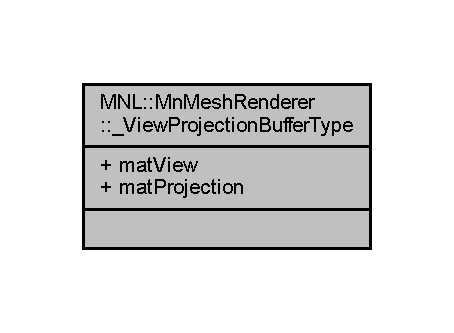
\includegraphics[width=218pt]{struct_m_n_l_1_1_mn_mesh_renderer_1_1___view_projection_buffer_type__coll__graph}
\end{center}
\end{figure}
\subsection*{Public 속성}
\begin{DoxyCompactItemize}
\item 
Direct\+X\+::\+Simple\+Math\+::\+Matrix \hyperlink{struct_m_n_l_1_1_mn_mesh_renderer_1_1___view_projection_buffer_type_af282f99d57500a4dc9e595adcddea495}{mat\+View}
\item 
Direct\+X\+::\+Simple\+Math\+::\+Matrix \hyperlink{struct_m_n_l_1_1_mn_mesh_renderer_1_1___view_projection_buffer_type_acb75b6be61aafc12dc66e68fd4da30ad}{mat\+Projection}
\end{DoxyCompactItemize}


\subsection{상세한 설명}


Mn\+Mesh\+Renderer.\+h 파일의 34 번째 라인에서 정의되었습니다.



\subsection{멤버 데이터 문서화}
\mbox{\Hypertarget{struct_m_n_l_1_1_mn_mesh_renderer_1_1___view_projection_buffer_type_acb75b6be61aafc12dc66e68fd4da30ad}\label{struct_m_n_l_1_1_mn_mesh_renderer_1_1___view_projection_buffer_type_acb75b6be61aafc12dc66e68fd4da30ad}} 
\index{M\+N\+L\+::\+Mn\+Mesh\+Renderer\+::\+\_\+\+View\+Projection\+Buffer\+Type@{M\+N\+L\+::\+Mn\+Mesh\+Renderer\+::\+\_\+\+View\+Projection\+Buffer\+Type}!mat\+Projection@{mat\+Projection}}
\index{mat\+Projection@{mat\+Projection}!M\+N\+L\+::\+Mn\+Mesh\+Renderer\+::\+\_\+\+View\+Projection\+Buffer\+Type@{M\+N\+L\+::\+Mn\+Mesh\+Renderer\+::\+\_\+\+View\+Projection\+Buffer\+Type}}
\subsubsection{\texorpdfstring{mat\+Projection}{matProjection}}
{\footnotesize\ttfamily Direct\+X\+::\+Simple\+Math\+::\+Matrix M\+N\+L\+::\+Mn\+Mesh\+Renderer\+::\+\_\+\+View\+Projection\+Buffer\+Type\+::mat\+Projection}



Mn\+Mesh\+Renderer.\+h 파일의 37 번째 라인에서 정의되었습니다.

\mbox{\Hypertarget{struct_m_n_l_1_1_mn_mesh_renderer_1_1___view_projection_buffer_type_af282f99d57500a4dc9e595adcddea495}\label{struct_m_n_l_1_1_mn_mesh_renderer_1_1___view_projection_buffer_type_af282f99d57500a4dc9e595adcddea495}} 
\index{M\+N\+L\+::\+Mn\+Mesh\+Renderer\+::\+\_\+\+View\+Projection\+Buffer\+Type@{M\+N\+L\+::\+Mn\+Mesh\+Renderer\+::\+\_\+\+View\+Projection\+Buffer\+Type}!mat\+View@{mat\+View}}
\index{mat\+View@{mat\+View}!M\+N\+L\+::\+Mn\+Mesh\+Renderer\+::\+\_\+\+View\+Projection\+Buffer\+Type@{M\+N\+L\+::\+Mn\+Mesh\+Renderer\+::\+\_\+\+View\+Projection\+Buffer\+Type}}
\subsubsection{\texorpdfstring{mat\+View}{matView}}
{\footnotesize\ttfamily Direct\+X\+::\+Simple\+Math\+::\+Matrix M\+N\+L\+::\+Mn\+Mesh\+Renderer\+::\+\_\+\+View\+Projection\+Buffer\+Type\+::mat\+View}



Mn\+Mesh\+Renderer.\+h 파일의 36 번째 라인에서 정의되었습니다.



이 구조체에 대한 문서화 페이지는 다음의 파일로부터 생성되었습니다.\+:\begin{DoxyCompactItemize}
\item 
Render/\hyperlink{_mn_mesh_renderer_8h}{Mn\+Mesh\+Renderer.\+h}\end{DoxyCompactItemize}

\hypertarget{struct_m_n_l_1_1_mn_skinned_mesh_renderer_1_1___view_projection_buffer_type}{}\section{M\+NL\+:\+:Mn\+Skinned\+Mesh\+Renderer\+:\+:\+\_\+\+View\+Projection\+Buffer\+Type 구조체 참조}
\label{struct_m_n_l_1_1_mn_skinned_mesh_renderer_1_1___view_projection_buffer_type}\index{M\+N\+L\+::\+Mn\+Skinned\+Mesh\+Renderer\+::\+\_\+\+View\+Projection\+Buffer\+Type@{M\+N\+L\+::\+Mn\+Skinned\+Mesh\+Renderer\+::\+\_\+\+View\+Projection\+Buffer\+Type}}


M\+NL\+:\+:Mn\+Skinned\+Mesh\+Renderer\+:\+:\+\_\+\+View\+Projection\+Buffer\+Type에 대한 협력 다이어그램\+:\nopagebreak
\begin{figure}[H]
\begin{center}
\leavevmode
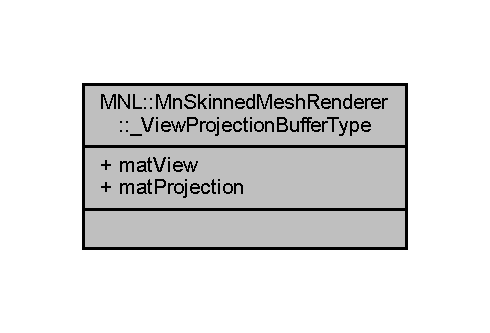
\includegraphics[width=235pt]{struct_m_n_l_1_1_mn_skinned_mesh_renderer_1_1___view_projection_buffer_type__coll__graph}
\end{center}
\end{figure}
\subsection*{Public 속성}
\begin{DoxyCompactItemize}
\item 
Direct\+X\+::\+Simple\+Math\+::\+Matrix \hyperlink{struct_m_n_l_1_1_mn_skinned_mesh_renderer_1_1___view_projection_buffer_type_a4bbebb4a794c138473e5ff50b62e1612}{mat\+View}
\item 
Direct\+X\+::\+Simple\+Math\+::\+Matrix \hyperlink{struct_m_n_l_1_1_mn_skinned_mesh_renderer_1_1___view_projection_buffer_type_abda3cf268206ff65417df2181bd08922}{mat\+Projection}
\end{DoxyCompactItemize}


\subsection{상세한 설명}


Mn\+Skinned\+Mesh\+Renderer.\+h 파일의 36 번째 라인에서 정의되었습니다.



\subsection{멤버 데이터 문서화}
\mbox{\Hypertarget{struct_m_n_l_1_1_mn_skinned_mesh_renderer_1_1___view_projection_buffer_type_abda3cf268206ff65417df2181bd08922}\label{struct_m_n_l_1_1_mn_skinned_mesh_renderer_1_1___view_projection_buffer_type_abda3cf268206ff65417df2181bd08922}} 
\index{M\+N\+L\+::\+Mn\+Skinned\+Mesh\+Renderer\+::\+\_\+\+View\+Projection\+Buffer\+Type@{M\+N\+L\+::\+Mn\+Skinned\+Mesh\+Renderer\+::\+\_\+\+View\+Projection\+Buffer\+Type}!mat\+Projection@{mat\+Projection}}
\index{mat\+Projection@{mat\+Projection}!M\+N\+L\+::\+Mn\+Skinned\+Mesh\+Renderer\+::\+\_\+\+View\+Projection\+Buffer\+Type@{M\+N\+L\+::\+Mn\+Skinned\+Mesh\+Renderer\+::\+\_\+\+View\+Projection\+Buffer\+Type}}
\subsubsection{\texorpdfstring{mat\+Projection}{matProjection}}
{\footnotesize\ttfamily Direct\+X\+::\+Simple\+Math\+::\+Matrix M\+N\+L\+::\+Mn\+Skinned\+Mesh\+Renderer\+::\+\_\+\+View\+Projection\+Buffer\+Type\+::mat\+Projection}



Mn\+Skinned\+Mesh\+Renderer.\+h 파일의 39 번째 라인에서 정의되었습니다.

\mbox{\Hypertarget{struct_m_n_l_1_1_mn_skinned_mesh_renderer_1_1___view_projection_buffer_type_a4bbebb4a794c138473e5ff50b62e1612}\label{struct_m_n_l_1_1_mn_skinned_mesh_renderer_1_1___view_projection_buffer_type_a4bbebb4a794c138473e5ff50b62e1612}} 
\index{M\+N\+L\+::\+Mn\+Skinned\+Mesh\+Renderer\+::\+\_\+\+View\+Projection\+Buffer\+Type@{M\+N\+L\+::\+Mn\+Skinned\+Mesh\+Renderer\+::\+\_\+\+View\+Projection\+Buffer\+Type}!mat\+View@{mat\+View}}
\index{mat\+View@{mat\+View}!M\+N\+L\+::\+Mn\+Skinned\+Mesh\+Renderer\+::\+\_\+\+View\+Projection\+Buffer\+Type@{M\+N\+L\+::\+Mn\+Skinned\+Mesh\+Renderer\+::\+\_\+\+View\+Projection\+Buffer\+Type}}
\subsubsection{\texorpdfstring{mat\+View}{matView}}
{\footnotesize\ttfamily Direct\+X\+::\+Simple\+Math\+::\+Matrix M\+N\+L\+::\+Mn\+Skinned\+Mesh\+Renderer\+::\+\_\+\+View\+Projection\+Buffer\+Type\+::mat\+View}



Mn\+Skinned\+Mesh\+Renderer.\+h 파일의 38 번째 라인에서 정의되었습니다.



이 구조체에 대한 문서화 페이지는 다음의 파일로부터 생성되었습니다.\+:\begin{DoxyCompactItemize}
\item 
Render/\hyperlink{_mn_skinned_mesh_renderer_8h}{Mn\+Skinned\+Mesh\+Renderer.\+h}\end{DoxyCompactItemize}

\hypertarget{struct_m_n_l_1_1_mn_mesh_renderer_1_1___world_buffer_type}{}\section{M\+NL\+:\+:Mn\+Mesh\+Renderer\+:\+:\+\_\+\+World\+Buffer\+Type 구조체 참조}
\label{struct_m_n_l_1_1_mn_mesh_renderer_1_1___world_buffer_type}\index{M\+N\+L\+::\+Mn\+Mesh\+Renderer\+::\+\_\+\+World\+Buffer\+Type@{M\+N\+L\+::\+Mn\+Mesh\+Renderer\+::\+\_\+\+World\+Buffer\+Type}}


M\+NL\+:\+:Mn\+Mesh\+Renderer\+:\+:\+\_\+\+World\+Buffer\+Type에 대한 협력 다이어그램\+:\nopagebreak
\begin{figure}[H]
\begin{center}
\leavevmode
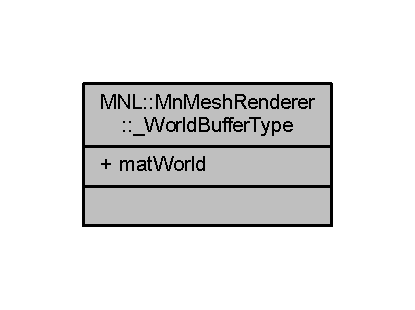
\includegraphics[width=199pt]{struct_m_n_l_1_1_mn_mesh_renderer_1_1___world_buffer_type__coll__graph}
\end{center}
\end{figure}
\subsection*{Public 속성}
\begin{DoxyCompactItemize}
\item 
Direct\+X\+::\+Simple\+Math\+::\+Matrix \hyperlink{struct_m_n_l_1_1_mn_mesh_renderer_1_1___world_buffer_type_a9ebb51c42f4e24827c51cd25c77daed4}{mat\+World}
\end{DoxyCompactItemize}


\subsection{상세한 설명}


Mn\+Mesh\+Renderer.\+h 파일의 30 번째 라인에서 정의되었습니다.



\subsection{멤버 데이터 문서화}
\mbox{\Hypertarget{struct_m_n_l_1_1_mn_mesh_renderer_1_1___world_buffer_type_a9ebb51c42f4e24827c51cd25c77daed4}\label{struct_m_n_l_1_1_mn_mesh_renderer_1_1___world_buffer_type_a9ebb51c42f4e24827c51cd25c77daed4}} 
\index{M\+N\+L\+::\+Mn\+Mesh\+Renderer\+::\+\_\+\+World\+Buffer\+Type@{M\+N\+L\+::\+Mn\+Mesh\+Renderer\+::\+\_\+\+World\+Buffer\+Type}!mat\+World@{mat\+World}}
\index{mat\+World@{mat\+World}!M\+N\+L\+::\+Mn\+Mesh\+Renderer\+::\+\_\+\+World\+Buffer\+Type@{M\+N\+L\+::\+Mn\+Mesh\+Renderer\+::\+\_\+\+World\+Buffer\+Type}}
\subsubsection{\texorpdfstring{mat\+World}{matWorld}}
{\footnotesize\ttfamily Direct\+X\+::\+Simple\+Math\+::\+Matrix M\+N\+L\+::\+Mn\+Mesh\+Renderer\+::\+\_\+\+World\+Buffer\+Type\+::mat\+World}



Mn\+Mesh\+Renderer.\+h 파일의 32 번째 라인에서 정의되었습니다.



이 구조체에 대한 문서화 페이지는 다음의 파일로부터 생성되었습니다.\+:\begin{DoxyCompactItemize}
\item 
Render/\hyperlink{_mn_mesh_renderer_8h}{Mn\+Mesh\+Renderer.\+h}\end{DoxyCompactItemize}

\hypertarget{struct_m_n_l_1_1_mn_skinned_mesh_renderer_1_1___world_buffer_type}{}\section{M\+NL\+:\+:Mn\+Skinned\+Mesh\+Renderer\+:\+:\+\_\+\+World\+Buffer\+Type 구조체 참조}
\label{struct_m_n_l_1_1_mn_skinned_mesh_renderer_1_1___world_buffer_type}\index{M\+N\+L\+::\+Mn\+Skinned\+Mesh\+Renderer\+::\+\_\+\+World\+Buffer\+Type@{M\+N\+L\+::\+Mn\+Skinned\+Mesh\+Renderer\+::\+\_\+\+World\+Buffer\+Type}}


M\+NL\+:\+:Mn\+Skinned\+Mesh\+Renderer\+:\+:\+\_\+\+World\+Buffer\+Type에 대한 협력 다이어그램\+:\nopagebreak
\begin{figure}[H]
\begin{center}
\leavevmode
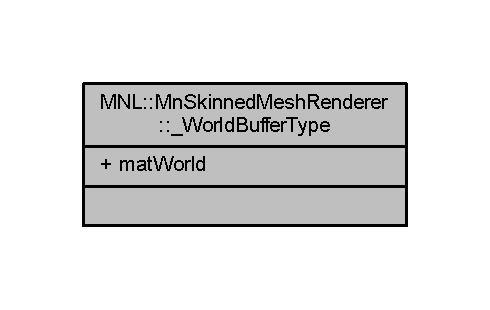
\includegraphics[width=235pt]{struct_m_n_l_1_1_mn_skinned_mesh_renderer_1_1___world_buffer_type__coll__graph}
\end{center}
\end{figure}
\subsection*{Public 속성}
\begin{DoxyCompactItemize}
\item 
Direct\+X\+::\+Simple\+Math\+::\+Matrix \hyperlink{struct_m_n_l_1_1_mn_skinned_mesh_renderer_1_1___world_buffer_type_a5c8d2b6785f90aa08047ab32dcfbe257}{mat\+World}
\end{DoxyCompactItemize}


\subsection{상세한 설명}


Mn\+Skinned\+Mesh\+Renderer.\+h 파일의 32 번째 라인에서 정의되었습니다.



\subsection{멤버 데이터 문서화}
\mbox{\Hypertarget{struct_m_n_l_1_1_mn_skinned_mesh_renderer_1_1___world_buffer_type_a5c8d2b6785f90aa08047ab32dcfbe257}\label{struct_m_n_l_1_1_mn_skinned_mesh_renderer_1_1___world_buffer_type_a5c8d2b6785f90aa08047ab32dcfbe257}} 
\index{M\+N\+L\+::\+Mn\+Skinned\+Mesh\+Renderer\+::\+\_\+\+World\+Buffer\+Type@{M\+N\+L\+::\+Mn\+Skinned\+Mesh\+Renderer\+::\+\_\+\+World\+Buffer\+Type}!mat\+World@{mat\+World}}
\index{mat\+World@{mat\+World}!M\+N\+L\+::\+Mn\+Skinned\+Mesh\+Renderer\+::\+\_\+\+World\+Buffer\+Type@{M\+N\+L\+::\+Mn\+Skinned\+Mesh\+Renderer\+::\+\_\+\+World\+Buffer\+Type}}
\subsubsection{\texorpdfstring{mat\+World}{matWorld}}
{\footnotesize\ttfamily Direct\+X\+::\+Simple\+Math\+::\+Matrix M\+N\+L\+::\+Mn\+Skinned\+Mesh\+Renderer\+::\+\_\+\+World\+Buffer\+Type\+::mat\+World}



Mn\+Skinned\+Mesh\+Renderer.\+h 파일의 34 번째 라인에서 정의되었습니다.



이 구조체에 대한 문서화 페이지는 다음의 파일로부터 생성되었습니다.\+:\begin{DoxyCompactItemize}
\item 
Render/\hyperlink{_mn_skinned_mesh_renderer_8h}{Mn\+Skinned\+Mesh\+Renderer.\+h}\end{DoxyCompactItemize}

\hypertarget{class_m_n_l_1_1_basic_shader_path}{}\section{M\+NL\+:\+:Basic\+Shader\+Path 클래스 참조}
\label{class_m_n_l_1_1_basic_shader_path}\index{M\+N\+L\+::\+Basic\+Shader\+Path@{M\+N\+L\+::\+Basic\+Shader\+Path}}


{\ttfamily \#include $<$Basic\+Shader\+Path.\+h$>$}



M\+NL\+:\+:Basic\+Shader\+Path에 대한 상속 다이어그램 \+: \nopagebreak
\begin{figure}[H]
\begin{center}
\leavevmode
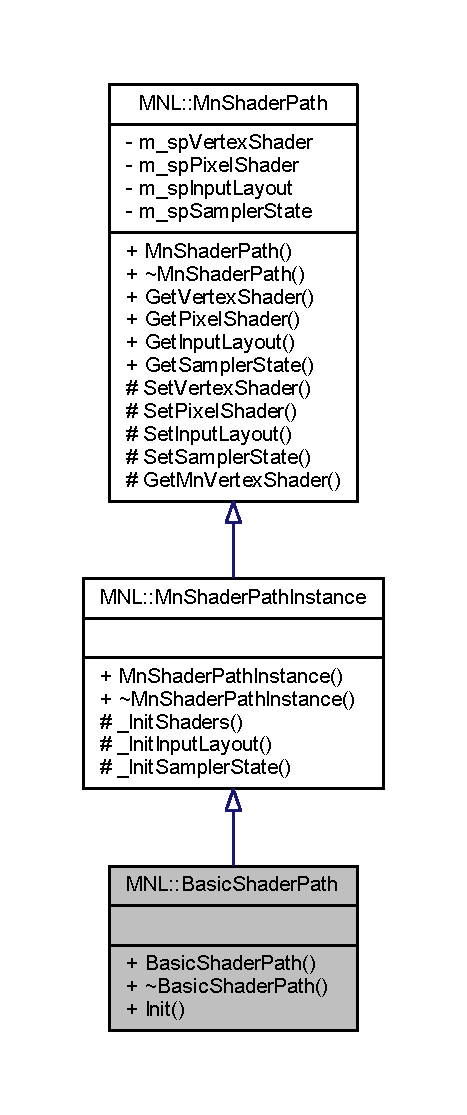
\includegraphics[width=224pt]{class_m_n_l_1_1_basic_shader_path__inherit__graph}
\end{center}
\end{figure}


M\+NL\+:\+:Basic\+Shader\+Path에 대한 협력 다이어그램\+:\nopagebreak
\begin{figure}[H]
\begin{center}
\leavevmode
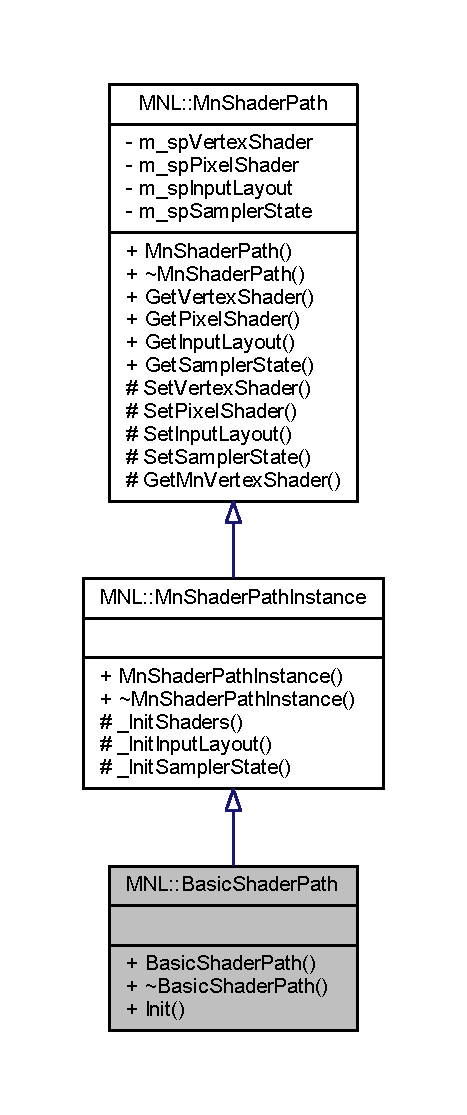
\includegraphics[width=224pt]{class_m_n_l_1_1_basic_shader_path__coll__graph}
\end{center}
\end{figure}
\subsection*{Public 멤버 함수}
\begin{DoxyCompactItemize}
\item 
\hyperlink{class_m_n_l_1_1_basic_shader_path_ae8908353c46de6669022661239c84b74}{Basic\+Shader\+Path} ()
\item 
\hyperlink{class_m_n_l_1_1_basic_shader_path_aa416c14988fdff0ecd7937bcec255ef7}{$\sim$\+Basic\+Shader\+Path} ()
\item 
H\+R\+E\+S\+U\+LT \hyperlink{class_m_n_l_1_1_basic_shader_path_a5600873eea14db77383ef1781c393aa9}{Init} (const \hyperlink{namespace_m_n_l_a1eec210db8f309a4a9ac0d9658784c31}{C\+P\+D3\+D\+Device} \&cp\+Device, const std\+::shared\+\_\+ptr$<$ \hyperlink{class_m_n_l_1_1_mn_custom_vertex_type}{Mn\+Custom\+Vertex\+Type} $>$ \&sp\+Vertex\+Type)
\end{DoxyCompactItemize}
\subsection*{추가로 상속된 멤버들}


\subsection{상세한 설명}


Basic\+Shader\+Path.\+h 파일의 9 번째 라인에서 정의되었습니다.



\subsection{생성자 \& 소멸자 문서화}
\mbox{\Hypertarget{class_m_n_l_1_1_basic_shader_path_ae8908353c46de6669022661239c84b74}\label{class_m_n_l_1_1_basic_shader_path_ae8908353c46de6669022661239c84b74}} 
\index{M\+N\+L\+::\+Basic\+Shader\+Path@{M\+N\+L\+::\+Basic\+Shader\+Path}!Basic\+Shader\+Path@{Basic\+Shader\+Path}}
\index{Basic\+Shader\+Path@{Basic\+Shader\+Path}!M\+N\+L\+::\+Basic\+Shader\+Path@{M\+N\+L\+::\+Basic\+Shader\+Path}}
\subsubsection{\texorpdfstring{Basic\+Shader\+Path()}{BasicShaderPath()}}
{\footnotesize\ttfamily Basic\+Shader\+Path\+::\+Basic\+Shader\+Path (\begin{DoxyParamCaption}{ }\end{DoxyParamCaption})}



Basic\+Shader\+Path.\+cpp 파일의 7 번째 라인에서 정의되었습니다.

\mbox{\Hypertarget{class_m_n_l_1_1_basic_shader_path_aa416c14988fdff0ecd7937bcec255ef7}\label{class_m_n_l_1_1_basic_shader_path_aa416c14988fdff0ecd7937bcec255ef7}} 
\index{M\+N\+L\+::\+Basic\+Shader\+Path@{M\+N\+L\+::\+Basic\+Shader\+Path}!````~Basic\+Shader\+Path@{$\sim$\+Basic\+Shader\+Path}}
\index{````~Basic\+Shader\+Path@{$\sim$\+Basic\+Shader\+Path}!M\+N\+L\+::\+Basic\+Shader\+Path@{M\+N\+L\+::\+Basic\+Shader\+Path}}
\subsubsection{\texorpdfstring{$\sim$\+Basic\+Shader\+Path()}{~BasicShaderPath()}}
{\footnotesize\ttfamily Basic\+Shader\+Path\+::$\sim$\+Basic\+Shader\+Path (\begin{DoxyParamCaption}{ }\end{DoxyParamCaption})}



Basic\+Shader\+Path.\+cpp 파일의 11 번째 라인에서 정의되었습니다.



\subsection{멤버 함수 문서화}
\mbox{\Hypertarget{class_m_n_l_1_1_basic_shader_path_a5600873eea14db77383ef1781c393aa9}\label{class_m_n_l_1_1_basic_shader_path_a5600873eea14db77383ef1781c393aa9}} 
\index{M\+N\+L\+::\+Basic\+Shader\+Path@{M\+N\+L\+::\+Basic\+Shader\+Path}!Init@{Init}}
\index{Init@{Init}!M\+N\+L\+::\+Basic\+Shader\+Path@{M\+N\+L\+::\+Basic\+Shader\+Path}}
\subsubsection{\texorpdfstring{Init()}{Init()}}
{\footnotesize\ttfamily H\+R\+E\+S\+U\+LT Basic\+Shader\+Path\+::\+Init (\begin{DoxyParamCaption}\item[{const \hyperlink{namespace_m_n_l_a1eec210db8f309a4a9ac0d9658784c31}{C\+P\+D3\+D\+Device} \&}]{cp\+Device,  }\item[{const std\+::shared\+\_\+ptr$<$ \hyperlink{class_m_n_l_1_1_mn_custom_vertex_type}{Mn\+Custom\+Vertex\+Type} $>$ \&}]{sp\+Vertex\+Type }\end{DoxyParamCaption})}



Basic\+Shader\+Path.\+cpp 파일의 18 번째 라인에서 정의되었습니다.



이 클래스에 대한 문서화 페이지는 다음의 파일들로부터 생성되었습니다.\+:\begin{DoxyCompactItemize}
\item 
\hyperlink{_basic_shader_path_8h}{Basic\+Shader\+Path.\+h}\item 
\hyperlink{_basic_shader_path_8cpp}{Basic\+Shader\+Path.\+cpp}\end{DoxyCompactItemize}

\hypertarget{class_m_n_l_1_1_mn_bone}{}\section{M\+NL\+:\+:Mn\+Bone 클래스 참조}
\label{class_m_n_l_1_1_mn_bone}\index{M\+N\+L\+::\+Mn\+Bone@{M\+N\+L\+::\+Mn\+Bone}}


{\ttfamily \#include $<$Mn\+Bone.\+h$>$}



M\+NL\+:\+:Mn\+Bone에 대한 협력 다이어그램\+:\nopagebreak
\begin{figure}[H]
\begin{center}
\leavevmode
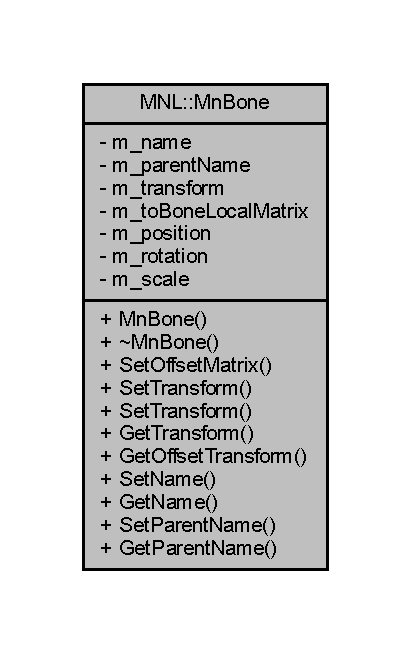
\includegraphics[width=197pt]{class_m_n_l_1_1_mn_bone__coll__graph}
\end{center}
\end{figure}
\subsection*{Public 멤버 함수}
\begin{DoxyCompactItemize}
\item 
\hyperlink{class_m_n_l_1_1_mn_bone_a2f2a084d73c21440e718c3a67a94355b}{Mn\+Bone} ()
\item 
\hyperlink{class_m_n_l_1_1_mn_bone_a56cefd0c1acf49770e49748fe2a3a51d}{$\sim$\+Mn\+Bone} ()
\item 
void \hyperlink{class_m_n_l_1_1_mn_bone_a523fe1078ba5b534b316d38748cb2625}{Set\+Offset\+Matrix} (const Direct\+X\+::\+Simple\+Math\+::\+Matrix \&offset\+Matrix)
\item 
void \hyperlink{class_m_n_l_1_1_mn_bone_a23ab583dd181a53935357ec51e376d9a}{Set\+Transform} (const Direct\+X\+::\+Simple\+Math\+::\+Matrix \&transform)
\item 
void \hyperlink{class_m_n_l_1_1_mn_bone_ad0b53762b81d65568955c67e59a7c845}{Set\+Transform} (const Direct\+X\+::\+Simple\+Math\+::\+Vector3 \&position, const Direct\+X\+::\+Simple\+Math\+::\+Quaternion \&rotation, const Direct\+X\+::\+Simple\+Math\+::\+Vector3 \&scale)
\item 
Direct\+X\+::\+Simple\+Math\+::\+Matrix \hyperlink{class_m_n_l_1_1_mn_bone_a404d1fc423d63715cd0a8bbe3afdaac7}{Get\+Transform} () const
\item 
Direct\+X\+::\+Simple\+Math\+::\+Matrix \hyperlink{class_m_n_l_1_1_mn_bone_a30963b69412919ada3ca5f166faf846f}{Get\+Offset\+Transform} () const
\item 
void \hyperlink{class_m_n_l_1_1_mn_bone_a36b9b60148969ce31bc74a4bbd4c56cf}{Set\+Name} (const std\+::string \&name)
\item 
std\+::string \hyperlink{class_m_n_l_1_1_mn_bone_a7780138cc897c4358c276cbe04c2868c}{Get\+Name} () const
\item 
void \hyperlink{class_m_n_l_1_1_mn_bone_a7be990cbdf3f123a6649b8de9968ac0f}{Set\+Parent\+Name} (const std\+::string \&parent\+Name)
\item 
std\+::string \hyperlink{class_m_n_l_1_1_mn_bone_a476cfd8bcfebded34cbcbfd08d6a44b2}{Get\+Parent\+Name} () const
\end{DoxyCompactItemize}
\subsection*{Private 속성}
\begin{DoxyCompactItemize}
\item 
std\+::string \hyperlink{class_m_n_l_1_1_mn_bone_adca6ae47b891bd0c63393a27f6c6eacb}{m\+\_\+name}
\item 
std\+::string \hyperlink{class_m_n_l_1_1_mn_bone_a73c16374ec9bd66ccb36d8a7f7a022ce}{m\+\_\+parent\+Name}
\item 
Direct\+X\+::\+Simple\+Math\+::\+Matrix \hyperlink{class_m_n_l_1_1_mn_bone_aea47d357de786e87817f49963ae22bea}{m\+\_\+transform}
\item 
Direct\+X\+::\+Simple\+Math\+::\+Matrix \hyperlink{class_m_n_l_1_1_mn_bone_a99bbff737e6e67c9be126bcf6be0c3b5}{m\+\_\+to\+Bone\+Local\+Matrix}
\item 
Direct\+X\+::\+Simple\+Math\+::\+Vector3 \hyperlink{class_m_n_l_1_1_mn_bone_a038566003fe128d05d36167353772701}{m\+\_\+position}
\item 
Direct\+X\+::\+Simple\+Math\+::\+Quaternion \hyperlink{class_m_n_l_1_1_mn_bone_ae891a94f5086aea0e3f136d54749dade}{m\+\_\+rotation}
\item 
Direct\+X\+::\+Simple\+Math\+::\+Vector3 \hyperlink{class_m_n_l_1_1_mn_bone_a7919dddae372b5511dc2adab951c6dc5}{m\+\_\+scale}
\end{DoxyCompactItemize}


\subsection{상세한 설명}


Mn\+Bone.\+h 파일의 13 번째 라인에서 정의되었습니다.



\subsection{생성자 \& 소멸자 문서화}
\mbox{\Hypertarget{class_m_n_l_1_1_mn_bone_a2f2a084d73c21440e718c3a67a94355b}\label{class_m_n_l_1_1_mn_bone_a2f2a084d73c21440e718c3a67a94355b}} 
\index{M\+N\+L\+::\+Mn\+Bone@{M\+N\+L\+::\+Mn\+Bone}!Mn\+Bone@{Mn\+Bone}}
\index{Mn\+Bone@{Mn\+Bone}!M\+N\+L\+::\+Mn\+Bone@{M\+N\+L\+::\+Mn\+Bone}}
\subsubsection{\texorpdfstring{Mn\+Bone()}{MnBone()}}
{\footnotesize\ttfamily Mn\+Bone\+::\+Mn\+Bone (\begin{DoxyParamCaption}{ }\end{DoxyParamCaption})}



Mn\+Bone.\+cpp 파일의 6 번째 라인에서 정의되었습니다.

\mbox{\Hypertarget{class_m_n_l_1_1_mn_bone_a56cefd0c1acf49770e49748fe2a3a51d}\label{class_m_n_l_1_1_mn_bone_a56cefd0c1acf49770e49748fe2a3a51d}} 
\index{M\+N\+L\+::\+Mn\+Bone@{M\+N\+L\+::\+Mn\+Bone}!````~Mn\+Bone@{$\sim$\+Mn\+Bone}}
\index{````~Mn\+Bone@{$\sim$\+Mn\+Bone}!M\+N\+L\+::\+Mn\+Bone@{M\+N\+L\+::\+Mn\+Bone}}
\subsubsection{\texorpdfstring{$\sim$\+Mn\+Bone()}{~MnBone()}}
{\footnotesize\ttfamily Mn\+Bone\+::$\sim$\+Mn\+Bone (\begin{DoxyParamCaption}{ }\end{DoxyParamCaption})}



Mn\+Bone.\+cpp 파일의 15 번째 라인에서 정의되었습니다.



\subsection{멤버 함수 문서화}
\mbox{\Hypertarget{class_m_n_l_1_1_mn_bone_a7780138cc897c4358c276cbe04c2868c}\label{class_m_n_l_1_1_mn_bone_a7780138cc897c4358c276cbe04c2868c}} 
\index{M\+N\+L\+::\+Mn\+Bone@{M\+N\+L\+::\+Mn\+Bone}!Get\+Name@{Get\+Name}}
\index{Get\+Name@{Get\+Name}!M\+N\+L\+::\+Mn\+Bone@{M\+N\+L\+::\+Mn\+Bone}}
\subsubsection{\texorpdfstring{Get\+Name()}{GetName()}}
{\footnotesize\ttfamily std\+::string Mn\+Bone\+::\+Get\+Name (\begin{DoxyParamCaption}{ }\end{DoxyParamCaption}) const}



Mn\+Bone.\+cpp 파일의 51 번째 라인에서 정의되었습니다.

\mbox{\Hypertarget{class_m_n_l_1_1_mn_bone_a30963b69412919ada3ca5f166faf846f}\label{class_m_n_l_1_1_mn_bone_a30963b69412919ada3ca5f166faf846f}} 
\index{M\+N\+L\+::\+Mn\+Bone@{M\+N\+L\+::\+Mn\+Bone}!Get\+Offset\+Transform@{Get\+Offset\+Transform}}
\index{Get\+Offset\+Transform@{Get\+Offset\+Transform}!M\+N\+L\+::\+Mn\+Bone@{M\+N\+L\+::\+Mn\+Bone}}
\subsubsection{\texorpdfstring{Get\+Offset\+Transform()}{GetOffsetTransform()}}
{\footnotesize\ttfamily Direct\+X\+::\+Simple\+Math\+::\+Matrix Mn\+Bone\+::\+Get\+Offset\+Transform (\begin{DoxyParamCaption}{ }\end{DoxyParamCaption}) const}



Mn\+Bone.\+cpp 파일의 42 번째 라인에서 정의되었습니다.

\mbox{\Hypertarget{class_m_n_l_1_1_mn_bone_a476cfd8bcfebded34cbcbfd08d6a44b2}\label{class_m_n_l_1_1_mn_bone_a476cfd8bcfebded34cbcbfd08d6a44b2}} 
\index{M\+N\+L\+::\+Mn\+Bone@{M\+N\+L\+::\+Mn\+Bone}!Get\+Parent\+Name@{Get\+Parent\+Name}}
\index{Get\+Parent\+Name@{Get\+Parent\+Name}!M\+N\+L\+::\+Mn\+Bone@{M\+N\+L\+::\+Mn\+Bone}}
\subsubsection{\texorpdfstring{Get\+Parent\+Name()}{GetParentName()}}
{\footnotesize\ttfamily std\+::string Mn\+Bone\+::\+Get\+Parent\+Name (\begin{DoxyParamCaption}{ }\end{DoxyParamCaption}) const}



Mn\+Bone.\+cpp 파일의 60 번째 라인에서 정의되었습니다.

\mbox{\Hypertarget{class_m_n_l_1_1_mn_bone_a404d1fc423d63715cd0a8bbe3afdaac7}\label{class_m_n_l_1_1_mn_bone_a404d1fc423d63715cd0a8bbe3afdaac7}} 
\index{M\+N\+L\+::\+Mn\+Bone@{M\+N\+L\+::\+Mn\+Bone}!Get\+Transform@{Get\+Transform}}
\index{Get\+Transform@{Get\+Transform}!M\+N\+L\+::\+Mn\+Bone@{M\+N\+L\+::\+Mn\+Bone}}
\subsubsection{\texorpdfstring{Get\+Transform()}{GetTransform()}}
{\footnotesize\ttfamily Direct\+X\+::\+Simple\+Math\+::\+Matrix Mn\+Bone\+::\+Get\+Transform (\begin{DoxyParamCaption}{ }\end{DoxyParamCaption}) const}

Get bone\textquotesingle{}s transformation from the mesh\textquotesingle{}s local space. Notice that the transformation is N\+OT R\+E\+L\+A\+T\+I\+VE TO I\+TS P\+A\+R\+E\+NT 

Mn\+Bone.\+cpp 파일의 38 번째 라인에서 정의되었습니다.

\mbox{\Hypertarget{class_m_n_l_1_1_mn_bone_a36b9b60148969ce31bc74a4bbd4c56cf}\label{class_m_n_l_1_1_mn_bone_a36b9b60148969ce31bc74a4bbd4c56cf}} 
\index{M\+N\+L\+::\+Mn\+Bone@{M\+N\+L\+::\+Mn\+Bone}!Set\+Name@{Set\+Name}}
\index{Set\+Name@{Set\+Name}!M\+N\+L\+::\+Mn\+Bone@{M\+N\+L\+::\+Mn\+Bone}}
\subsubsection{\texorpdfstring{Set\+Name()}{SetName()}}
{\footnotesize\ttfamily void Mn\+Bone\+::\+Set\+Name (\begin{DoxyParamCaption}\item[{const std\+::string \&}]{name }\end{DoxyParamCaption})}



Mn\+Bone.\+cpp 파일의 46 번째 라인에서 정의되었습니다.

\mbox{\Hypertarget{class_m_n_l_1_1_mn_bone_a523fe1078ba5b534b316d38748cb2625}\label{class_m_n_l_1_1_mn_bone_a523fe1078ba5b534b316d38748cb2625}} 
\index{M\+N\+L\+::\+Mn\+Bone@{M\+N\+L\+::\+Mn\+Bone}!Set\+Offset\+Matrix@{Set\+Offset\+Matrix}}
\index{Set\+Offset\+Matrix@{Set\+Offset\+Matrix}!M\+N\+L\+::\+Mn\+Bone@{M\+N\+L\+::\+Mn\+Bone}}
\subsubsection{\texorpdfstring{Set\+Offset\+Matrix()}{SetOffsetMatrix()}}
{\footnotesize\ttfamily void Mn\+Bone\+::\+Set\+Offset\+Matrix (\begin{DoxyParamCaption}\item[{const Direct\+X\+::\+Simple\+Math\+::\+Matrix \&}]{offset\+Matrix }\end{DoxyParamCaption})}

Set mesh space to bone\textquotesingle{}s local space matrix 

Mn\+Bone.\+cpp 파일의 19 번째 라인에서 정의되었습니다.

\mbox{\Hypertarget{class_m_n_l_1_1_mn_bone_a7be990cbdf3f123a6649b8de9968ac0f}\label{class_m_n_l_1_1_mn_bone_a7be990cbdf3f123a6649b8de9968ac0f}} 
\index{M\+N\+L\+::\+Mn\+Bone@{M\+N\+L\+::\+Mn\+Bone}!Set\+Parent\+Name@{Set\+Parent\+Name}}
\index{Set\+Parent\+Name@{Set\+Parent\+Name}!M\+N\+L\+::\+Mn\+Bone@{M\+N\+L\+::\+Mn\+Bone}}
\subsubsection{\texorpdfstring{Set\+Parent\+Name()}{SetParentName()}}
{\footnotesize\ttfamily void Mn\+Bone\+::\+Set\+Parent\+Name (\begin{DoxyParamCaption}\item[{const std\+::string \&}]{parent\+Name }\end{DoxyParamCaption})}



Mn\+Bone.\+cpp 파일의 56 번째 라인에서 정의되었습니다.

\mbox{\Hypertarget{class_m_n_l_1_1_mn_bone_a23ab583dd181a53935357ec51e376d9a}\label{class_m_n_l_1_1_mn_bone_a23ab583dd181a53935357ec51e376d9a}} 
\index{M\+N\+L\+::\+Mn\+Bone@{M\+N\+L\+::\+Mn\+Bone}!Set\+Transform@{Set\+Transform}}
\index{Set\+Transform@{Set\+Transform}!M\+N\+L\+::\+Mn\+Bone@{M\+N\+L\+::\+Mn\+Bone}}
\subsubsection{\texorpdfstring{Set\+Transform()}{SetTransform()}\hspace{0.1cm}{\footnotesize\ttfamily [1/2]}}
{\footnotesize\ttfamily void Mn\+Bone\+::\+Set\+Transform (\begin{DoxyParamCaption}\item[{const Direct\+X\+::\+Simple\+Math\+::\+Matrix \&}]{transform }\end{DoxyParamCaption})}



Mn\+Bone.\+cpp 파일의 23 번째 라인에서 정의되었습니다.

\mbox{\Hypertarget{class_m_n_l_1_1_mn_bone_ad0b53762b81d65568955c67e59a7c845}\label{class_m_n_l_1_1_mn_bone_ad0b53762b81d65568955c67e59a7c845}} 
\index{M\+N\+L\+::\+Mn\+Bone@{M\+N\+L\+::\+Mn\+Bone}!Set\+Transform@{Set\+Transform}}
\index{Set\+Transform@{Set\+Transform}!M\+N\+L\+::\+Mn\+Bone@{M\+N\+L\+::\+Mn\+Bone}}
\subsubsection{\texorpdfstring{Set\+Transform()}{SetTransform()}\hspace{0.1cm}{\footnotesize\ttfamily [2/2]}}
{\footnotesize\ttfamily void M\+N\+L\+::\+Mn\+Bone\+::\+Set\+Transform (\begin{DoxyParamCaption}\item[{const Direct\+X\+::\+Simple\+Math\+::\+Vector3 \&}]{position,  }\item[{const Direct\+X\+::\+Simple\+Math\+::\+Quaternion \&}]{rotation,  }\item[{const Direct\+X\+::\+Simple\+Math\+::\+Vector3 \&}]{scale }\end{DoxyParamCaption})}



Mn\+Bone.\+cpp 파일의 29 번째 라인에서 정의되었습니다.



\subsection{멤버 데이터 문서화}
\mbox{\Hypertarget{class_m_n_l_1_1_mn_bone_adca6ae47b891bd0c63393a27f6c6eacb}\label{class_m_n_l_1_1_mn_bone_adca6ae47b891bd0c63393a27f6c6eacb}} 
\index{M\+N\+L\+::\+Mn\+Bone@{M\+N\+L\+::\+Mn\+Bone}!m\+\_\+name@{m\+\_\+name}}
\index{m\+\_\+name@{m\+\_\+name}!M\+N\+L\+::\+Mn\+Bone@{M\+N\+L\+::\+Mn\+Bone}}
\subsubsection{\texorpdfstring{m\+\_\+name}{m\_name}}
{\footnotesize\ttfamily std\+::string M\+N\+L\+::\+Mn\+Bone\+::m\+\_\+name\hspace{0.3cm}{\ttfamily [private]}}



Mn\+Bone.\+h 파일의 39 번째 라인에서 정의되었습니다.

\mbox{\Hypertarget{class_m_n_l_1_1_mn_bone_a73c16374ec9bd66ccb36d8a7f7a022ce}\label{class_m_n_l_1_1_mn_bone_a73c16374ec9bd66ccb36d8a7f7a022ce}} 
\index{M\+N\+L\+::\+Mn\+Bone@{M\+N\+L\+::\+Mn\+Bone}!m\+\_\+parent\+Name@{m\+\_\+parent\+Name}}
\index{m\+\_\+parent\+Name@{m\+\_\+parent\+Name}!M\+N\+L\+::\+Mn\+Bone@{M\+N\+L\+::\+Mn\+Bone}}
\subsubsection{\texorpdfstring{m\+\_\+parent\+Name}{m\_parentName}}
{\footnotesize\ttfamily std\+::string M\+N\+L\+::\+Mn\+Bone\+::m\+\_\+parent\+Name\hspace{0.3cm}{\ttfamily [private]}}



Mn\+Bone.\+h 파일의 40 번째 라인에서 정의되었습니다.

\mbox{\Hypertarget{class_m_n_l_1_1_mn_bone_a038566003fe128d05d36167353772701}\label{class_m_n_l_1_1_mn_bone_a038566003fe128d05d36167353772701}} 
\index{M\+N\+L\+::\+Mn\+Bone@{M\+N\+L\+::\+Mn\+Bone}!m\+\_\+position@{m\+\_\+position}}
\index{m\+\_\+position@{m\+\_\+position}!M\+N\+L\+::\+Mn\+Bone@{M\+N\+L\+::\+Mn\+Bone}}
\subsubsection{\texorpdfstring{m\+\_\+position}{m\_position}}
{\footnotesize\ttfamily Direct\+X\+::\+Simple\+Math\+::\+Vector3 M\+N\+L\+::\+Mn\+Bone\+::m\+\_\+position\hspace{0.3cm}{\ttfamily [private]}}



Mn\+Bone.\+h 파일의 43 번째 라인에서 정의되었습니다.

\mbox{\Hypertarget{class_m_n_l_1_1_mn_bone_ae891a94f5086aea0e3f136d54749dade}\label{class_m_n_l_1_1_mn_bone_ae891a94f5086aea0e3f136d54749dade}} 
\index{M\+N\+L\+::\+Mn\+Bone@{M\+N\+L\+::\+Mn\+Bone}!m\+\_\+rotation@{m\+\_\+rotation}}
\index{m\+\_\+rotation@{m\+\_\+rotation}!M\+N\+L\+::\+Mn\+Bone@{M\+N\+L\+::\+Mn\+Bone}}
\subsubsection{\texorpdfstring{m\+\_\+rotation}{m\_rotation}}
{\footnotesize\ttfamily Direct\+X\+::\+Simple\+Math\+::\+Quaternion M\+N\+L\+::\+Mn\+Bone\+::m\+\_\+rotation\hspace{0.3cm}{\ttfamily [private]}}



Mn\+Bone.\+h 파일의 44 번째 라인에서 정의되었습니다.

\mbox{\Hypertarget{class_m_n_l_1_1_mn_bone_a7919dddae372b5511dc2adab951c6dc5}\label{class_m_n_l_1_1_mn_bone_a7919dddae372b5511dc2adab951c6dc5}} 
\index{M\+N\+L\+::\+Mn\+Bone@{M\+N\+L\+::\+Mn\+Bone}!m\+\_\+scale@{m\+\_\+scale}}
\index{m\+\_\+scale@{m\+\_\+scale}!M\+N\+L\+::\+Mn\+Bone@{M\+N\+L\+::\+Mn\+Bone}}
\subsubsection{\texorpdfstring{m\+\_\+scale}{m\_scale}}
{\footnotesize\ttfamily Direct\+X\+::\+Simple\+Math\+::\+Vector3 M\+N\+L\+::\+Mn\+Bone\+::m\+\_\+scale\hspace{0.3cm}{\ttfamily [private]}}



Mn\+Bone.\+h 파일의 45 번째 라인에서 정의되었습니다.

\mbox{\Hypertarget{class_m_n_l_1_1_mn_bone_a99bbff737e6e67c9be126bcf6be0c3b5}\label{class_m_n_l_1_1_mn_bone_a99bbff737e6e67c9be126bcf6be0c3b5}} 
\index{M\+N\+L\+::\+Mn\+Bone@{M\+N\+L\+::\+Mn\+Bone}!m\+\_\+to\+Bone\+Local\+Matrix@{m\+\_\+to\+Bone\+Local\+Matrix}}
\index{m\+\_\+to\+Bone\+Local\+Matrix@{m\+\_\+to\+Bone\+Local\+Matrix}!M\+N\+L\+::\+Mn\+Bone@{M\+N\+L\+::\+Mn\+Bone}}
\subsubsection{\texorpdfstring{m\+\_\+to\+Bone\+Local\+Matrix}{m\_toBoneLocalMatrix}}
{\footnotesize\ttfamily Direct\+X\+::\+Simple\+Math\+::\+Matrix M\+N\+L\+::\+Mn\+Bone\+::m\+\_\+to\+Bone\+Local\+Matrix\hspace{0.3cm}{\ttfamily [private]}}



Mn\+Bone.\+h 파일의 42 번째 라인에서 정의되었습니다.

\mbox{\Hypertarget{class_m_n_l_1_1_mn_bone_aea47d357de786e87817f49963ae22bea}\label{class_m_n_l_1_1_mn_bone_aea47d357de786e87817f49963ae22bea}} 
\index{M\+N\+L\+::\+Mn\+Bone@{M\+N\+L\+::\+Mn\+Bone}!m\+\_\+transform@{m\+\_\+transform}}
\index{m\+\_\+transform@{m\+\_\+transform}!M\+N\+L\+::\+Mn\+Bone@{M\+N\+L\+::\+Mn\+Bone}}
\subsubsection{\texorpdfstring{m\+\_\+transform}{m\_transform}}
{\footnotesize\ttfamily Direct\+X\+::\+Simple\+Math\+::\+Matrix M\+N\+L\+::\+Mn\+Bone\+::m\+\_\+transform\hspace{0.3cm}{\ttfamily [private]}}



Mn\+Bone.\+h 파일의 41 번째 라인에서 정의되었습니다.



이 클래스에 대한 문서화 페이지는 다음의 파일들로부터 생성되었습니다.\+:\begin{DoxyCompactItemize}
\item 
Render/\hyperlink{_mn_bone_8h}{Mn\+Bone.\+h}\item 
Render/\hyperlink{_mn_bone_8cpp}{Mn\+Bone.\+cpp}\end{DoxyCompactItemize}

\hypertarget{class_m_n_l_1_1_mn_bone_animation}{}\section{M\+NL\+:\+:Mn\+Bone\+Animation 클래스 참조}
\label{class_m_n_l_1_1_mn_bone_animation}\index{M\+N\+L\+::\+Mn\+Bone\+Animation@{M\+N\+L\+::\+Mn\+Bone\+Animation}}


{\ttfamily \#include $<$Mn\+Bone\+Animation.\+h$>$}



M\+NL\+:\+:Mn\+Bone\+Animation에 대한 협력 다이어그램\+:\nopagebreak
\begin{figure}[H]
\begin{center}
\leavevmode
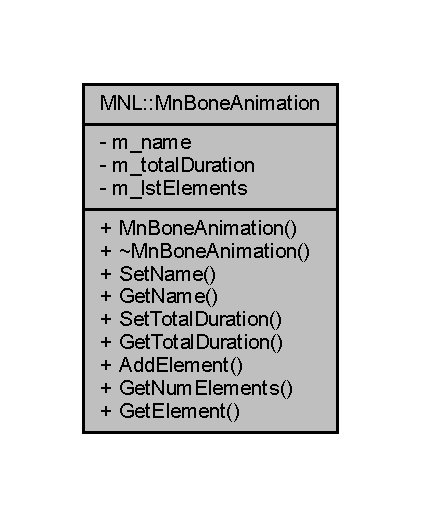
\includegraphics[width=202pt]{class_m_n_l_1_1_mn_bone_animation__coll__graph}
\end{center}
\end{figure}
\subsection*{Public 멤버 함수}
\begin{DoxyCompactItemize}
\item 
\hyperlink{class_m_n_l_1_1_mn_bone_animation_a13e19925c530a41833bef5b0bf19606a}{Mn\+Bone\+Animation} ()
\item 
\hyperlink{class_m_n_l_1_1_mn_bone_animation_a42386108606a71f25a9516620cc71bab}{$\sim$\+Mn\+Bone\+Animation} ()
\item 
void \hyperlink{class_m_n_l_1_1_mn_bone_animation_a9761262aa92163949e863423b4124cec}{Set\+Name} (const std\+::string \&name)
\item 
const std\+::string \& \hyperlink{class_m_n_l_1_1_mn_bone_animation_a4b6860d0100f2af61ecd035acbbdcd5e}{Get\+Name} () const
\item 
void \hyperlink{class_m_n_l_1_1_mn_bone_animation_a05eb549b3556fa7e355d36c0314cf024}{Set\+Total\+Duration} (double duration)
\item 
double \hyperlink{class_m_n_l_1_1_mn_bone_animation_a40f42c23266fe578394b127d34eb8208}{Get\+Total\+Duration} () const
\item 
void \hyperlink{class_m_n_l_1_1_mn_bone_animation_a77c33ae5a73412609e51eb681863e2a5}{Add\+Element} (const \hyperlink{class_m_n_l_1_1_mn_bone_animation_element}{Mn\+Bone\+Animation\+Element} \&key\+Frame)
\item 
U\+I\+NT \hyperlink{class_m_n_l_1_1_mn_bone_animation_a4ab001675acbda970c1a9b41b886d76f}{Get\+Num\+Elements} () const
\item 
\hyperlink{class_m_n_l_1_1_mn_bone_animation_element}{Mn\+Bone\+Animation\+Element} \hyperlink{class_m_n_l_1_1_mn_bone_animation_a8a40906cb4103fe6c926b439ad847e74}{Get\+Element} (U\+I\+NT index) const
\end{DoxyCompactItemize}
\subsection*{Private 속성}
\begin{DoxyCompactItemize}
\item 
std\+::string \hyperlink{class_m_n_l_1_1_mn_bone_animation_a87c5e79d5169c58db4fb0a581333eefc}{m\+\_\+name}
\item 
double \hyperlink{class_m_n_l_1_1_mn_bone_animation_a01d7e4fb6175d5492b699473df7a9650}{m\+\_\+total\+Duration}
\item 
std\+::vector$<$ \hyperlink{class_m_n_l_1_1_mn_bone_animation_element}{Mn\+Bone\+Animation\+Element} $>$ \hyperlink{class_m_n_l_1_1_mn_bone_animation_ac5e2681c430e633aec0e020f3e03354a}{m\+\_\+lst\+Elements}
\end{DoxyCompactItemize}


\subsection{상세한 설명}


Mn\+Bone\+Animation.\+h 파일의 9 번째 라인에서 정의되었습니다.



\subsection{생성자 \& 소멸자 문서화}
\mbox{\Hypertarget{class_m_n_l_1_1_mn_bone_animation_a13e19925c530a41833bef5b0bf19606a}\label{class_m_n_l_1_1_mn_bone_animation_a13e19925c530a41833bef5b0bf19606a}} 
\index{M\+N\+L\+::\+Mn\+Bone\+Animation@{M\+N\+L\+::\+Mn\+Bone\+Animation}!Mn\+Bone\+Animation@{Mn\+Bone\+Animation}}
\index{Mn\+Bone\+Animation@{Mn\+Bone\+Animation}!M\+N\+L\+::\+Mn\+Bone\+Animation@{M\+N\+L\+::\+Mn\+Bone\+Animation}}
\subsubsection{\texorpdfstring{Mn\+Bone\+Animation()}{MnBoneAnimation()}}
{\footnotesize\ttfamily Mn\+Bone\+Animation\+::\+Mn\+Bone\+Animation (\begin{DoxyParamCaption}{ }\end{DoxyParamCaption})}



Mn\+Bone\+Animation.\+cpp 파일의 5 번째 라인에서 정의되었습니다.

\mbox{\Hypertarget{class_m_n_l_1_1_mn_bone_animation_a42386108606a71f25a9516620cc71bab}\label{class_m_n_l_1_1_mn_bone_animation_a42386108606a71f25a9516620cc71bab}} 
\index{M\+N\+L\+::\+Mn\+Bone\+Animation@{M\+N\+L\+::\+Mn\+Bone\+Animation}!````~Mn\+Bone\+Animation@{$\sim$\+Mn\+Bone\+Animation}}
\index{````~Mn\+Bone\+Animation@{$\sim$\+Mn\+Bone\+Animation}!M\+N\+L\+::\+Mn\+Bone\+Animation@{M\+N\+L\+::\+Mn\+Bone\+Animation}}
\subsubsection{\texorpdfstring{$\sim$\+Mn\+Bone\+Animation()}{~MnBoneAnimation()}}
{\footnotesize\ttfamily Mn\+Bone\+Animation\+::$\sim$\+Mn\+Bone\+Animation (\begin{DoxyParamCaption}{ }\end{DoxyParamCaption})}



Mn\+Bone\+Animation.\+cpp 파일의 9 번째 라인에서 정의되었습니다.



\subsection{멤버 함수 문서화}
\mbox{\Hypertarget{class_m_n_l_1_1_mn_bone_animation_a77c33ae5a73412609e51eb681863e2a5}\label{class_m_n_l_1_1_mn_bone_animation_a77c33ae5a73412609e51eb681863e2a5}} 
\index{M\+N\+L\+::\+Mn\+Bone\+Animation@{M\+N\+L\+::\+Mn\+Bone\+Animation}!Add\+Element@{Add\+Element}}
\index{Add\+Element@{Add\+Element}!M\+N\+L\+::\+Mn\+Bone\+Animation@{M\+N\+L\+::\+Mn\+Bone\+Animation}}
\subsubsection{\texorpdfstring{Add\+Element()}{AddElement()}}
{\footnotesize\ttfamily void Mn\+Bone\+Animation\+::\+Add\+Element (\begin{DoxyParamCaption}\item[{const \hyperlink{class_m_n_l_1_1_mn_bone_animation_element}{Mn\+Bone\+Animation\+Element} \&}]{key\+Frame }\end{DoxyParamCaption})}



Mn\+Bone\+Animation.\+cpp 파일의 29 번째 라인에서 정의되었습니다.

\mbox{\Hypertarget{class_m_n_l_1_1_mn_bone_animation_a8a40906cb4103fe6c926b439ad847e74}\label{class_m_n_l_1_1_mn_bone_animation_a8a40906cb4103fe6c926b439ad847e74}} 
\index{M\+N\+L\+::\+Mn\+Bone\+Animation@{M\+N\+L\+::\+Mn\+Bone\+Animation}!Get\+Element@{Get\+Element}}
\index{Get\+Element@{Get\+Element}!M\+N\+L\+::\+Mn\+Bone\+Animation@{M\+N\+L\+::\+Mn\+Bone\+Animation}}
\subsubsection{\texorpdfstring{Get\+Element()}{GetElement()}}
{\footnotesize\ttfamily \hyperlink{class_m_n_l_1_1_mn_bone_animation_element}{Mn\+Bone\+Animation\+Element} Mn\+Bone\+Animation\+::\+Get\+Element (\begin{DoxyParamCaption}\item[{U\+I\+NT}]{index }\end{DoxyParamCaption}) const}



Mn\+Bone\+Animation.\+cpp 파일의 38 번째 라인에서 정의되었습니다.

\mbox{\Hypertarget{class_m_n_l_1_1_mn_bone_animation_a4b6860d0100f2af61ecd035acbbdcd5e}\label{class_m_n_l_1_1_mn_bone_animation_a4b6860d0100f2af61ecd035acbbdcd5e}} 
\index{M\+N\+L\+::\+Mn\+Bone\+Animation@{M\+N\+L\+::\+Mn\+Bone\+Animation}!Get\+Name@{Get\+Name}}
\index{Get\+Name@{Get\+Name}!M\+N\+L\+::\+Mn\+Bone\+Animation@{M\+N\+L\+::\+Mn\+Bone\+Animation}}
\subsubsection{\texorpdfstring{Get\+Name()}{GetName()}}
{\footnotesize\ttfamily const std\+::string \& Mn\+Bone\+Animation\+::\+Get\+Name (\begin{DoxyParamCaption}{ }\end{DoxyParamCaption}) const}



Mn\+Bone\+Animation.\+cpp 파일의 17 번째 라인에서 정의되었습니다.

\mbox{\Hypertarget{class_m_n_l_1_1_mn_bone_animation_a4ab001675acbda970c1a9b41b886d76f}\label{class_m_n_l_1_1_mn_bone_animation_a4ab001675acbda970c1a9b41b886d76f}} 
\index{M\+N\+L\+::\+Mn\+Bone\+Animation@{M\+N\+L\+::\+Mn\+Bone\+Animation}!Get\+Num\+Elements@{Get\+Num\+Elements}}
\index{Get\+Num\+Elements@{Get\+Num\+Elements}!M\+N\+L\+::\+Mn\+Bone\+Animation@{M\+N\+L\+::\+Mn\+Bone\+Animation}}
\subsubsection{\texorpdfstring{Get\+Num\+Elements()}{GetNumElements()}}
{\footnotesize\ttfamily U\+I\+NT Mn\+Bone\+Animation\+::\+Get\+Num\+Elements (\begin{DoxyParamCaption}{ }\end{DoxyParamCaption}) const}



Mn\+Bone\+Animation.\+cpp 파일의 33 번째 라인에서 정의되었습니다.

\mbox{\Hypertarget{class_m_n_l_1_1_mn_bone_animation_a40f42c23266fe578394b127d34eb8208}\label{class_m_n_l_1_1_mn_bone_animation_a40f42c23266fe578394b127d34eb8208}} 
\index{M\+N\+L\+::\+Mn\+Bone\+Animation@{M\+N\+L\+::\+Mn\+Bone\+Animation}!Get\+Total\+Duration@{Get\+Total\+Duration}}
\index{Get\+Total\+Duration@{Get\+Total\+Duration}!M\+N\+L\+::\+Mn\+Bone\+Animation@{M\+N\+L\+::\+Mn\+Bone\+Animation}}
\subsubsection{\texorpdfstring{Get\+Total\+Duration()}{GetTotalDuration()}}
{\footnotesize\ttfamily double Mn\+Bone\+Animation\+::\+Get\+Total\+Duration (\begin{DoxyParamCaption}{ }\end{DoxyParamCaption}) const}



Mn\+Bone\+Animation.\+cpp 파일의 25 번째 라인에서 정의되었습니다.

\mbox{\Hypertarget{class_m_n_l_1_1_mn_bone_animation_a9761262aa92163949e863423b4124cec}\label{class_m_n_l_1_1_mn_bone_animation_a9761262aa92163949e863423b4124cec}} 
\index{M\+N\+L\+::\+Mn\+Bone\+Animation@{M\+N\+L\+::\+Mn\+Bone\+Animation}!Set\+Name@{Set\+Name}}
\index{Set\+Name@{Set\+Name}!M\+N\+L\+::\+Mn\+Bone\+Animation@{M\+N\+L\+::\+Mn\+Bone\+Animation}}
\subsubsection{\texorpdfstring{Set\+Name()}{SetName()}}
{\footnotesize\ttfamily void Mn\+Bone\+Animation\+::\+Set\+Name (\begin{DoxyParamCaption}\item[{const std\+::string \&}]{name }\end{DoxyParamCaption})}



Mn\+Bone\+Animation.\+cpp 파일의 13 번째 라인에서 정의되었습니다.

\mbox{\Hypertarget{class_m_n_l_1_1_mn_bone_animation_a05eb549b3556fa7e355d36c0314cf024}\label{class_m_n_l_1_1_mn_bone_animation_a05eb549b3556fa7e355d36c0314cf024}} 
\index{M\+N\+L\+::\+Mn\+Bone\+Animation@{M\+N\+L\+::\+Mn\+Bone\+Animation}!Set\+Total\+Duration@{Set\+Total\+Duration}}
\index{Set\+Total\+Duration@{Set\+Total\+Duration}!M\+N\+L\+::\+Mn\+Bone\+Animation@{M\+N\+L\+::\+Mn\+Bone\+Animation}}
\subsubsection{\texorpdfstring{Set\+Total\+Duration()}{SetTotalDuration()}}
{\footnotesize\ttfamily void Mn\+Bone\+Animation\+::\+Set\+Total\+Duration (\begin{DoxyParamCaption}\item[{double}]{duration }\end{DoxyParamCaption})}



Mn\+Bone\+Animation.\+cpp 파일의 21 번째 라인에서 정의되었습니다.



\subsection{멤버 데이터 문서화}
\mbox{\Hypertarget{class_m_n_l_1_1_mn_bone_animation_ac5e2681c430e633aec0e020f3e03354a}\label{class_m_n_l_1_1_mn_bone_animation_ac5e2681c430e633aec0e020f3e03354a}} 
\index{M\+N\+L\+::\+Mn\+Bone\+Animation@{M\+N\+L\+::\+Mn\+Bone\+Animation}!m\+\_\+lst\+Elements@{m\+\_\+lst\+Elements}}
\index{m\+\_\+lst\+Elements@{m\+\_\+lst\+Elements}!M\+N\+L\+::\+Mn\+Bone\+Animation@{M\+N\+L\+::\+Mn\+Bone\+Animation}}
\subsubsection{\texorpdfstring{m\+\_\+lst\+Elements}{m\_lstElements}}
{\footnotesize\ttfamily std\+::vector$<$\hyperlink{class_m_n_l_1_1_mn_bone_animation_element}{Mn\+Bone\+Animation\+Element}$>$ M\+N\+L\+::\+Mn\+Bone\+Animation\+::m\+\_\+lst\+Elements\hspace{0.3cm}{\ttfamily [private]}}



Mn\+Bone\+Animation.\+h 파일의 28 번째 라인에서 정의되었습니다.

\mbox{\Hypertarget{class_m_n_l_1_1_mn_bone_animation_a87c5e79d5169c58db4fb0a581333eefc}\label{class_m_n_l_1_1_mn_bone_animation_a87c5e79d5169c58db4fb0a581333eefc}} 
\index{M\+N\+L\+::\+Mn\+Bone\+Animation@{M\+N\+L\+::\+Mn\+Bone\+Animation}!m\+\_\+name@{m\+\_\+name}}
\index{m\+\_\+name@{m\+\_\+name}!M\+N\+L\+::\+Mn\+Bone\+Animation@{M\+N\+L\+::\+Mn\+Bone\+Animation}}
\subsubsection{\texorpdfstring{m\+\_\+name}{m\_name}}
{\footnotesize\ttfamily std\+::string M\+N\+L\+::\+Mn\+Bone\+Animation\+::m\+\_\+name\hspace{0.3cm}{\ttfamily [private]}}



Mn\+Bone\+Animation.\+h 파일의 26 번째 라인에서 정의되었습니다.

\mbox{\Hypertarget{class_m_n_l_1_1_mn_bone_animation_a01d7e4fb6175d5492b699473df7a9650}\label{class_m_n_l_1_1_mn_bone_animation_a01d7e4fb6175d5492b699473df7a9650}} 
\index{M\+N\+L\+::\+Mn\+Bone\+Animation@{M\+N\+L\+::\+Mn\+Bone\+Animation}!m\+\_\+total\+Duration@{m\+\_\+total\+Duration}}
\index{m\+\_\+total\+Duration@{m\+\_\+total\+Duration}!M\+N\+L\+::\+Mn\+Bone\+Animation@{M\+N\+L\+::\+Mn\+Bone\+Animation}}
\subsubsection{\texorpdfstring{m\+\_\+total\+Duration}{m\_totalDuration}}
{\footnotesize\ttfamily double M\+N\+L\+::\+Mn\+Bone\+Animation\+::m\+\_\+total\+Duration\hspace{0.3cm}{\ttfamily [private]}}



Mn\+Bone\+Animation.\+h 파일의 27 번째 라인에서 정의되었습니다.



이 클래스에 대한 문서화 페이지는 다음의 파일들로부터 생성되었습니다.\+:\begin{DoxyCompactItemize}
\item 
Render/\hyperlink{_mn_bone_animation_8h}{Mn\+Bone\+Animation.\+h}\item 
Render/\hyperlink{_mn_bone_animation_8cpp}{Mn\+Bone\+Animation.\+cpp}\end{DoxyCompactItemize}

\hypertarget{class_m_n_l_1_1_mn_bone_animation_element}{}\section{M\+NL\+:\+:Mn\+Bone\+Animation\+Element 클래스 참조}
\label{class_m_n_l_1_1_mn_bone_animation_element}\index{M\+N\+L\+::\+Mn\+Bone\+Animation\+Element@{M\+N\+L\+::\+Mn\+Bone\+Animation\+Element}}


{\ttfamily \#include $<$Mn\+Bone\+Animation\+Element.\+h$>$}



M\+NL\+:\+:Mn\+Bone\+Animation\+Element에 대한 협력 다이어그램\+:\nopagebreak
\begin{figure}[H]
\begin{center}
\leavevmode
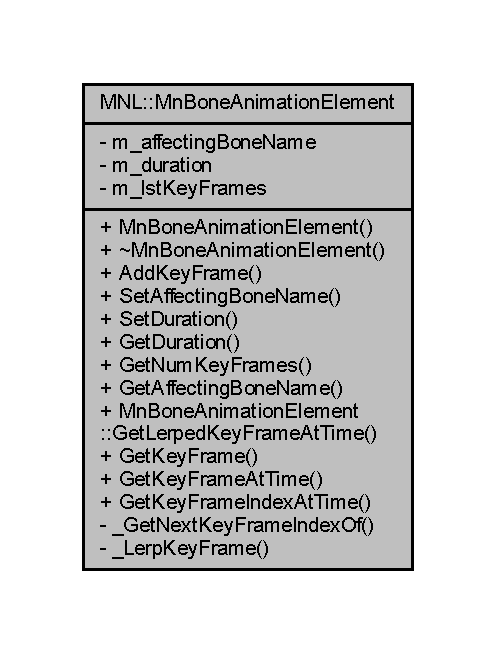
\includegraphics[width=238pt]{class_m_n_l_1_1_mn_bone_animation_element__coll__graph}
\end{center}
\end{figure}
\subsection*{Public 멤버 함수}
\begin{DoxyCompactItemize}
\item 
\hyperlink{class_m_n_l_1_1_mn_bone_animation_element_a17a71367d88886a9a1a06ce72cc3ae3f}{Mn\+Bone\+Animation\+Element} ()
\item 
\hyperlink{class_m_n_l_1_1_mn_bone_animation_element_a485d435a1d1a7ba730721c06ebfa0df5}{$\sim$\+Mn\+Bone\+Animation\+Element} ()
\item 
void \hyperlink{class_m_n_l_1_1_mn_bone_animation_element_a3c4b8bf56a5c5ebf5d6045ae93e5b808}{Add\+Key\+Frame} (const \hyperlink{struct_m_n_l_1_1_mn_bone_animation_key_frame}{Mn\+Bone\+Animation\+Key\+Frame} \&key)
\item 
void \hyperlink{class_m_n_l_1_1_mn_bone_animation_element_a9e9864a75d577193b3e39ce56838c43c}{Set\+Affecting\+Bone\+Name} (const std\+::string \&affecting\+Bone\+Name)
\item 
void \hyperlink{class_m_n_l_1_1_mn_bone_animation_element_a2f9f402279191cf7009e8b47bf3f3311}{Set\+Duration} (double duration)
\item 
double \hyperlink{class_m_n_l_1_1_mn_bone_animation_element_ad489dc7c72dea26d157a205d6af4fadb}{Get\+Duration} () const
\item 
U\+I\+NT \hyperlink{class_m_n_l_1_1_mn_bone_animation_element_ac92bc52d44e187e00af032d5faa5c735}{Get\+Num\+Key\+Frames} () const
\item 
std\+::string \hyperlink{class_m_n_l_1_1_mn_bone_animation_element_a7461a3a8bf2078d394db3a86c3a5eda6}{Get\+Affecting\+Bone\+Name} () const
\item 
\hyperlink{struct_m_n_l_1_1_mn_bone_animation_key_frame}{Mn\+Bone\+Animation\+Key\+Frame} \hyperlink{class_m_n_l_1_1_mn_bone_animation_element_ab689fa5a0df4c1d6a601baa13759d10d}{Mn\+Bone\+Animation\+Element\+::\+Get\+Lerped\+Key\+Frame\+At\+Time} (float time\+Factor)
\item 
\hyperlink{struct_m_n_l_1_1_mn_bone_animation_key_frame}{Mn\+Bone\+Animation\+Key\+Frame} \hyperlink{class_m_n_l_1_1_mn_bone_animation_element_a8cd10f7f60f232471e6ce603cdbf76ea}{Get\+Key\+Frame} (U\+I\+NT index) const
\item 
\hyperlink{struct_m_n_l_1_1_mn_bone_animation_key_frame}{Mn\+Bone\+Animation\+Key\+Frame} \hyperlink{class_m_n_l_1_1_mn_bone_animation_element_a58874b3fe81886f1c13ca6f77b4a171c}{Get\+Key\+Frame\+At\+Time} (float time\+Factor) const
\item 
U\+I\+NT \hyperlink{class_m_n_l_1_1_mn_bone_animation_element_ad22dfccb49a16ee30ab83c2ca0ca3185}{Get\+Key\+Frame\+Index\+At\+Time} (float time\+Factor) const
\end{DoxyCompactItemize}
\subsection*{Private 멤버 함수}
\begin{DoxyCompactItemize}
\item 
U\+I\+NT \hyperlink{class_m_n_l_1_1_mn_bone_animation_element_ae0385d67d5f8663fd2a7e398e8e2f91e}{\+\_\+\+Get\+Next\+Key\+Frame\+Index\+Of} (U\+I\+NT current\+Index) const
\item 
\hyperlink{struct_m_n_l_1_1_mn_bone_animation_key_frame}{Mn\+Bone\+Animation\+Key\+Frame} \hyperlink{class_m_n_l_1_1_mn_bone_animation_element_a3e789fbdea899e545eb5ff7a3aa41961}{\+\_\+\+Lerp\+Key\+Frame} (const \hyperlink{struct_m_n_l_1_1_mn_bone_animation_key_frame}{Mn\+Bone\+Animation\+Key\+Frame} \&key\+Frame\+\_\+from, const \hyperlink{struct_m_n_l_1_1_mn_bone_animation_key_frame}{Mn\+Bone\+Animation\+Key\+Frame} \&key\+Frame\+\_\+to, float factor)
\end{DoxyCompactItemize}
\subsection*{Private 속성}
\begin{DoxyCompactItemize}
\item 
std\+::string \hyperlink{class_m_n_l_1_1_mn_bone_animation_element_af8bc9d470a35c8d41283660baa36ecaf}{m\+\_\+affecting\+Bone\+Name}
\item 
double \hyperlink{class_m_n_l_1_1_mn_bone_animation_element_ad6427e5172eb3a5754f133dbda4fa43c}{m\+\_\+duration}
\item 
std\+::vector$<$ \hyperlink{struct_m_n_l_1_1_mn_bone_animation_key_frame}{Mn\+Bone\+Animation\+Key\+Frame} $>$ \hyperlink{class_m_n_l_1_1_mn_bone_animation_element_adb31ea7e47450a243d3b87ceadab86d0}{m\+\_\+lst\+Key\+Frames}
\end{DoxyCompactItemize}


\subsection{상세한 설명}


Mn\+Bone\+Animation\+Element.\+h 파일의 21 번째 라인에서 정의되었습니다.



\subsection{생성자 \& 소멸자 문서화}
\mbox{\Hypertarget{class_m_n_l_1_1_mn_bone_animation_element_a17a71367d88886a9a1a06ce72cc3ae3f}\label{class_m_n_l_1_1_mn_bone_animation_element_a17a71367d88886a9a1a06ce72cc3ae3f}} 
\index{M\+N\+L\+::\+Mn\+Bone\+Animation\+Element@{M\+N\+L\+::\+Mn\+Bone\+Animation\+Element}!Mn\+Bone\+Animation\+Element@{Mn\+Bone\+Animation\+Element}}
\index{Mn\+Bone\+Animation\+Element@{Mn\+Bone\+Animation\+Element}!M\+N\+L\+::\+Mn\+Bone\+Animation\+Element@{M\+N\+L\+::\+Mn\+Bone\+Animation\+Element}}
\subsubsection{\texorpdfstring{Mn\+Bone\+Animation\+Element()}{MnBoneAnimationElement()}}
{\footnotesize\ttfamily Mn\+Bone\+Animation\+Element\+::\+Mn\+Bone\+Animation\+Element (\begin{DoxyParamCaption}{ }\end{DoxyParamCaption})}



Mn\+Bone\+Animation\+Element.\+cpp 파일의 6 번째 라인에서 정의되었습니다.

\mbox{\Hypertarget{class_m_n_l_1_1_mn_bone_animation_element_a485d435a1d1a7ba730721c06ebfa0df5}\label{class_m_n_l_1_1_mn_bone_animation_element_a485d435a1d1a7ba730721c06ebfa0df5}} 
\index{M\+N\+L\+::\+Mn\+Bone\+Animation\+Element@{M\+N\+L\+::\+Mn\+Bone\+Animation\+Element}!````~Mn\+Bone\+Animation\+Element@{$\sim$\+Mn\+Bone\+Animation\+Element}}
\index{````~Mn\+Bone\+Animation\+Element@{$\sim$\+Mn\+Bone\+Animation\+Element}!M\+N\+L\+::\+Mn\+Bone\+Animation\+Element@{M\+N\+L\+::\+Mn\+Bone\+Animation\+Element}}
\subsubsection{\texorpdfstring{$\sim$\+Mn\+Bone\+Animation\+Element()}{~MnBoneAnimationElement()}}
{\footnotesize\ttfamily Mn\+Bone\+Animation\+Element\+::$\sim$\+Mn\+Bone\+Animation\+Element (\begin{DoxyParamCaption}{ }\end{DoxyParamCaption})}



Mn\+Bone\+Animation\+Element.\+cpp 파일의 10 번째 라인에서 정의되었습니다.



\subsection{멤버 함수 문서화}
\mbox{\Hypertarget{class_m_n_l_1_1_mn_bone_animation_element_ae0385d67d5f8663fd2a7e398e8e2f91e}\label{class_m_n_l_1_1_mn_bone_animation_element_ae0385d67d5f8663fd2a7e398e8e2f91e}} 
\index{M\+N\+L\+::\+Mn\+Bone\+Animation\+Element@{M\+N\+L\+::\+Mn\+Bone\+Animation\+Element}!\+\_\+\+Get\+Next\+Key\+Frame\+Index\+Of@{\+\_\+\+Get\+Next\+Key\+Frame\+Index\+Of}}
\index{\+\_\+\+Get\+Next\+Key\+Frame\+Index\+Of@{\+\_\+\+Get\+Next\+Key\+Frame\+Index\+Of}!M\+N\+L\+::\+Mn\+Bone\+Animation\+Element@{M\+N\+L\+::\+Mn\+Bone\+Animation\+Element}}
\subsubsection{\texorpdfstring{\+\_\+\+Get\+Next\+Key\+Frame\+Index\+Of()}{\_GetNextKeyFrameIndexOf()}}
{\footnotesize\ttfamily U\+I\+NT Mn\+Bone\+Animation\+Element\+::\+\_\+\+Get\+Next\+Key\+Frame\+Index\+Of (\begin{DoxyParamCaption}\item[{U\+I\+NT}]{current\+Index }\end{DoxyParamCaption}) const\hspace{0.3cm}{\ttfamily [private]}}



Mn\+Bone\+Animation\+Element.\+cpp 파일의 94 번째 라인에서 정의되었습니다.

\mbox{\Hypertarget{class_m_n_l_1_1_mn_bone_animation_element_a3e789fbdea899e545eb5ff7a3aa41961}\label{class_m_n_l_1_1_mn_bone_animation_element_a3e789fbdea899e545eb5ff7a3aa41961}} 
\index{M\+N\+L\+::\+Mn\+Bone\+Animation\+Element@{M\+N\+L\+::\+Mn\+Bone\+Animation\+Element}!\+\_\+\+Lerp\+Key\+Frame@{\+\_\+\+Lerp\+Key\+Frame}}
\index{\+\_\+\+Lerp\+Key\+Frame@{\+\_\+\+Lerp\+Key\+Frame}!M\+N\+L\+::\+Mn\+Bone\+Animation\+Element@{M\+N\+L\+::\+Mn\+Bone\+Animation\+Element}}
\subsubsection{\texorpdfstring{\+\_\+\+Lerp\+Key\+Frame()}{\_LerpKeyFrame()}}
{\footnotesize\ttfamily \hyperlink{struct_m_n_l_1_1_mn_bone_animation_key_frame}{Mn\+Bone\+Animation\+Key\+Frame} Mn\+Bone\+Animation\+Element\+::\+\_\+\+Lerp\+Key\+Frame (\begin{DoxyParamCaption}\item[{const \hyperlink{struct_m_n_l_1_1_mn_bone_animation_key_frame}{Mn\+Bone\+Animation\+Key\+Frame} \&}]{key\+Frame\+\_\+from,  }\item[{const \hyperlink{struct_m_n_l_1_1_mn_bone_animation_key_frame}{Mn\+Bone\+Animation\+Key\+Frame} \&}]{key\+Frame\+\_\+to,  }\item[{float}]{factor }\end{DoxyParamCaption})\hspace{0.3cm}{\ttfamily [private]}}



Mn\+Bone\+Animation\+Element.\+cpp 파일의 104 번째 라인에서 정의되었습니다.

\mbox{\Hypertarget{class_m_n_l_1_1_mn_bone_animation_element_a3c4b8bf56a5c5ebf5d6045ae93e5b808}\label{class_m_n_l_1_1_mn_bone_animation_element_a3c4b8bf56a5c5ebf5d6045ae93e5b808}} 
\index{M\+N\+L\+::\+Mn\+Bone\+Animation\+Element@{M\+N\+L\+::\+Mn\+Bone\+Animation\+Element}!Add\+Key\+Frame@{Add\+Key\+Frame}}
\index{Add\+Key\+Frame@{Add\+Key\+Frame}!M\+N\+L\+::\+Mn\+Bone\+Animation\+Element@{M\+N\+L\+::\+Mn\+Bone\+Animation\+Element}}
\subsubsection{\texorpdfstring{Add\+Key\+Frame()}{AddKeyFrame()}}
{\footnotesize\ttfamily void Mn\+Bone\+Animation\+Element\+::\+Add\+Key\+Frame (\begin{DoxyParamCaption}\item[{const \hyperlink{struct_m_n_l_1_1_mn_bone_animation_key_frame}{Mn\+Bone\+Animation\+Key\+Frame} \&}]{key }\end{DoxyParamCaption})}



Mn\+Bone\+Animation\+Element.\+cpp 파일의 14 번째 라인에서 정의되었습니다.

\mbox{\Hypertarget{class_m_n_l_1_1_mn_bone_animation_element_a7461a3a8bf2078d394db3a86c3a5eda6}\label{class_m_n_l_1_1_mn_bone_animation_element_a7461a3a8bf2078d394db3a86c3a5eda6}} 
\index{M\+N\+L\+::\+Mn\+Bone\+Animation\+Element@{M\+N\+L\+::\+Mn\+Bone\+Animation\+Element}!Get\+Affecting\+Bone\+Name@{Get\+Affecting\+Bone\+Name}}
\index{Get\+Affecting\+Bone\+Name@{Get\+Affecting\+Bone\+Name}!M\+N\+L\+::\+Mn\+Bone\+Animation\+Element@{M\+N\+L\+::\+Mn\+Bone\+Animation\+Element}}
\subsubsection{\texorpdfstring{Get\+Affecting\+Bone\+Name()}{GetAffectingBoneName()}}
{\footnotesize\ttfamily std\+::string Mn\+Bone\+Animation\+Element\+::\+Get\+Affecting\+Bone\+Name (\begin{DoxyParamCaption}{ }\end{DoxyParamCaption}) const}



Mn\+Bone\+Animation\+Element.\+cpp 파일의 39 번째 라인에서 정의되었습니다.

\mbox{\Hypertarget{class_m_n_l_1_1_mn_bone_animation_element_ad489dc7c72dea26d157a205d6af4fadb}\label{class_m_n_l_1_1_mn_bone_animation_element_ad489dc7c72dea26d157a205d6af4fadb}} 
\index{M\+N\+L\+::\+Mn\+Bone\+Animation\+Element@{M\+N\+L\+::\+Mn\+Bone\+Animation\+Element}!Get\+Duration@{Get\+Duration}}
\index{Get\+Duration@{Get\+Duration}!M\+N\+L\+::\+Mn\+Bone\+Animation\+Element@{M\+N\+L\+::\+Mn\+Bone\+Animation\+Element}}
\subsubsection{\texorpdfstring{Get\+Duration()}{GetDuration()}}
{\footnotesize\ttfamily double Mn\+Bone\+Animation\+Element\+::\+Get\+Duration (\begin{DoxyParamCaption}{ }\end{DoxyParamCaption}) const}



Mn\+Bone\+Animation\+Element.\+cpp 파일의 31 번째 라인에서 정의되었습니다.

\mbox{\Hypertarget{class_m_n_l_1_1_mn_bone_animation_element_a8cd10f7f60f232471e6ce603cdbf76ea}\label{class_m_n_l_1_1_mn_bone_animation_element_a8cd10f7f60f232471e6ce603cdbf76ea}} 
\index{M\+N\+L\+::\+Mn\+Bone\+Animation\+Element@{M\+N\+L\+::\+Mn\+Bone\+Animation\+Element}!Get\+Key\+Frame@{Get\+Key\+Frame}}
\index{Get\+Key\+Frame@{Get\+Key\+Frame}!M\+N\+L\+::\+Mn\+Bone\+Animation\+Element@{M\+N\+L\+::\+Mn\+Bone\+Animation\+Element}}
\subsubsection{\texorpdfstring{Get\+Key\+Frame()}{GetKeyFrame()}}
{\footnotesize\ttfamily \hyperlink{struct_m_n_l_1_1_mn_bone_animation_key_frame}{Mn\+Bone\+Animation\+Key\+Frame} Mn\+Bone\+Animation\+Element\+::\+Get\+Key\+Frame (\begin{DoxyParamCaption}\item[{U\+I\+NT}]{index }\end{DoxyParamCaption}) const}

Get key frame at the index 

Mn\+Bone\+Animation\+Element.\+cpp 파일의 22 번째 라인에서 정의되었습니다.

\mbox{\Hypertarget{class_m_n_l_1_1_mn_bone_animation_element_a58874b3fe81886f1c13ca6f77b4a171c}\label{class_m_n_l_1_1_mn_bone_animation_element_a58874b3fe81886f1c13ca6f77b4a171c}} 
\index{M\+N\+L\+::\+Mn\+Bone\+Animation\+Element@{M\+N\+L\+::\+Mn\+Bone\+Animation\+Element}!Get\+Key\+Frame\+At\+Time@{Get\+Key\+Frame\+At\+Time}}
\index{Get\+Key\+Frame\+At\+Time@{Get\+Key\+Frame\+At\+Time}!M\+N\+L\+::\+Mn\+Bone\+Animation\+Element@{M\+N\+L\+::\+Mn\+Bone\+Animation\+Element}}
\subsubsection{\texorpdfstring{Get\+Key\+Frame\+At\+Time()}{GetKeyFrameAtTime()}}
{\footnotesize\ttfamily \hyperlink{struct_m_n_l_1_1_mn_bone_animation_key_frame}{Mn\+Bone\+Animation\+Key\+Frame} Mn\+Bone\+Animation\+Element\+::\+Get\+Key\+Frame\+At\+Time (\begin{DoxyParamCaption}\item[{float}]{time\+Factor }\end{DoxyParamCaption}) const}

Get key frame at the specific time. 
\begin{DoxyParams}{매개변수}
{\em time\+Factor} & must be 0.\+0 $\sim$ 1.\+0. Calculated by (target\+Tick)/(total\+Tick) \\
\hline
\end{DoxyParams}
\begin{DoxyReturn}{반환값}
empty key frame if it has no key frames 
\end{DoxyReturn}


Mn\+Bone\+Animation\+Element.\+cpp 파일의 65 번째 라인에서 정의되었습니다.

\mbox{\Hypertarget{class_m_n_l_1_1_mn_bone_animation_element_ad22dfccb49a16ee30ab83c2ca0ca3185}\label{class_m_n_l_1_1_mn_bone_animation_element_ad22dfccb49a16ee30ab83c2ca0ca3185}} 
\index{M\+N\+L\+::\+Mn\+Bone\+Animation\+Element@{M\+N\+L\+::\+Mn\+Bone\+Animation\+Element}!Get\+Key\+Frame\+Index\+At\+Time@{Get\+Key\+Frame\+Index\+At\+Time}}
\index{Get\+Key\+Frame\+Index\+At\+Time@{Get\+Key\+Frame\+Index\+At\+Time}!M\+N\+L\+::\+Mn\+Bone\+Animation\+Element@{M\+N\+L\+::\+Mn\+Bone\+Animation\+Element}}
\subsubsection{\texorpdfstring{Get\+Key\+Frame\+Index\+At\+Time()}{GetKeyFrameIndexAtTime()}}
{\footnotesize\ttfamily U\+I\+NT Mn\+Bone\+Animation\+Element\+::\+Get\+Key\+Frame\+Index\+At\+Time (\begin{DoxyParamCaption}\item[{float}]{time\+Factor }\end{DoxyParamCaption}) const}

Get key frame\textquotesingle{}s index at the specific time. 
\begin{DoxyParams}{매개변수}
{\em time\+Factor} & must be 0.\+0 $\sim$ 1.\+0. Calculated by (target\+Tick)/(total\+Tick) \\
\hline
\end{DoxyParams}
\begin{DoxyReturn}{반환값}
empty key frame if it has no key frames 
\end{DoxyReturn}


Mn\+Bone\+Animation\+Element.\+cpp 파일의 74 번째 라인에서 정의되었습니다.

\mbox{\Hypertarget{class_m_n_l_1_1_mn_bone_animation_element_ac92bc52d44e187e00af032d5faa5c735}\label{class_m_n_l_1_1_mn_bone_animation_element_ac92bc52d44e187e00af032d5faa5c735}} 
\index{M\+N\+L\+::\+Mn\+Bone\+Animation\+Element@{M\+N\+L\+::\+Mn\+Bone\+Animation\+Element}!Get\+Num\+Key\+Frames@{Get\+Num\+Key\+Frames}}
\index{Get\+Num\+Key\+Frames@{Get\+Num\+Key\+Frames}!M\+N\+L\+::\+Mn\+Bone\+Animation\+Element@{M\+N\+L\+::\+Mn\+Bone\+Animation\+Element}}
\subsubsection{\texorpdfstring{Get\+Num\+Key\+Frames()}{GetNumKeyFrames()}}
{\footnotesize\ttfamily U\+I\+NT Mn\+Bone\+Animation\+Element\+::\+Get\+Num\+Key\+Frames (\begin{DoxyParamCaption}{ }\end{DoxyParamCaption}) const}



Mn\+Bone\+Animation\+Element.\+cpp 파일의 35 번째 라인에서 정의되었습니다.

\mbox{\Hypertarget{class_m_n_l_1_1_mn_bone_animation_element_ab689fa5a0df4c1d6a601baa13759d10d}\label{class_m_n_l_1_1_mn_bone_animation_element_ab689fa5a0df4c1d6a601baa13759d10d}} 
\index{M\+N\+L\+::\+Mn\+Bone\+Animation\+Element@{M\+N\+L\+::\+Mn\+Bone\+Animation\+Element}!Mn\+Bone\+Animation\+Element\+::\+Get\+Lerped\+Key\+Frame\+At\+Time@{Mn\+Bone\+Animation\+Element\+::\+Get\+Lerped\+Key\+Frame\+At\+Time}}
\index{Mn\+Bone\+Animation\+Element\+::\+Get\+Lerped\+Key\+Frame\+At\+Time@{Mn\+Bone\+Animation\+Element\+::\+Get\+Lerped\+Key\+Frame\+At\+Time}!M\+N\+L\+::\+Mn\+Bone\+Animation\+Element@{M\+N\+L\+::\+Mn\+Bone\+Animation\+Element}}
\subsubsection{\texorpdfstring{Mn\+Bone\+Animation\+Element\+::\+Get\+Lerped\+Key\+Frame\+At\+Time()}{MnBoneAnimationElement::GetLerpedKeyFrameAtTime()}}
{\footnotesize\ttfamily \hyperlink{struct_m_n_l_1_1_mn_bone_animation_key_frame}{Mn\+Bone\+Animation\+Key\+Frame} M\+N\+L\+::\+Mn\+Bone\+Animation\+Element\+::\+Mn\+Bone\+Animation\+Element\+::\+Get\+Lerped\+Key\+Frame\+At\+Time (\begin{DoxyParamCaption}\item[{float}]{time\+Factor }\end{DoxyParamCaption})}

Get automatically lerped key frame at the specific time. 
\begin{DoxyParams}{매개변수}
{\em time\+Factor} & must be 0.\+0 $\sim$ 1.\+0. Calculated by (target\+Tick)/(total\+Tick) \\
\hline
\end{DoxyParams}
\begin{DoxyReturn}{반환값}
empty key frame if it has no key frames 
\end{DoxyReturn}
\mbox{\Hypertarget{class_m_n_l_1_1_mn_bone_animation_element_a9e9864a75d577193b3e39ce56838c43c}\label{class_m_n_l_1_1_mn_bone_animation_element_a9e9864a75d577193b3e39ce56838c43c}} 
\index{M\+N\+L\+::\+Mn\+Bone\+Animation\+Element@{M\+N\+L\+::\+Mn\+Bone\+Animation\+Element}!Set\+Affecting\+Bone\+Name@{Set\+Affecting\+Bone\+Name}}
\index{Set\+Affecting\+Bone\+Name@{Set\+Affecting\+Bone\+Name}!M\+N\+L\+::\+Mn\+Bone\+Animation\+Element@{M\+N\+L\+::\+Mn\+Bone\+Animation\+Element}}
\subsubsection{\texorpdfstring{Set\+Affecting\+Bone\+Name()}{SetAffectingBoneName()}}
{\footnotesize\ttfamily void Mn\+Bone\+Animation\+Element\+::\+Set\+Affecting\+Bone\+Name (\begin{DoxyParamCaption}\item[{const std\+::string \&}]{affecting\+Bone\+Name }\end{DoxyParamCaption})}



Mn\+Bone\+Animation\+Element.\+cpp 파일의 18 번째 라인에서 정의되었습니다.

\mbox{\Hypertarget{class_m_n_l_1_1_mn_bone_animation_element_a2f9f402279191cf7009e8b47bf3f3311}\label{class_m_n_l_1_1_mn_bone_animation_element_a2f9f402279191cf7009e8b47bf3f3311}} 
\index{M\+N\+L\+::\+Mn\+Bone\+Animation\+Element@{M\+N\+L\+::\+Mn\+Bone\+Animation\+Element}!Set\+Duration@{Set\+Duration}}
\index{Set\+Duration@{Set\+Duration}!M\+N\+L\+::\+Mn\+Bone\+Animation\+Element@{M\+N\+L\+::\+Mn\+Bone\+Animation\+Element}}
\subsubsection{\texorpdfstring{Set\+Duration()}{SetDuration()}}
{\footnotesize\ttfamily void Mn\+Bone\+Animation\+Element\+::\+Set\+Duration (\begin{DoxyParamCaption}\item[{double}]{duration }\end{DoxyParamCaption})}



Mn\+Bone\+Animation\+Element.\+cpp 파일의 26 번째 라인에서 정의되었습니다.



\subsection{멤버 데이터 문서화}
\mbox{\Hypertarget{class_m_n_l_1_1_mn_bone_animation_element_af8bc9d470a35c8d41283660baa36ecaf}\label{class_m_n_l_1_1_mn_bone_animation_element_af8bc9d470a35c8d41283660baa36ecaf}} 
\index{M\+N\+L\+::\+Mn\+Bone\+Animation\+Element@{M\+N\+L\+::\+Mn\+Bone\+Animation\+Element}!m\+\_\+affecting\+Bone\+Name@{m\+\_\+affecting\+Bone\+Name}}
\index{m\+\_\+affecting\+Bone\+Name@{m\+\_\+affecting\+Bone\+Name}!M\+N\+L\+::\+Mn\+Bone\+Animation\+Element@{M\+N\+L\+::\+Mn\+Bone\+Animation\+Element}}
\subsubsection{\texorpdfstring{m\+\_\+affecting\+Bone\+Name}{m\_affectingBoneName}}
{\footnotesize\ttfamily std\+::string M\+N\+L\+::\+Mn\+Bone\+Animation\+Element\+::m\+\_\+affecting\+Bone\+Name\hspace{0.3cm}{\ttfamily [private]}}



Mn\+Bone\+Animation\+Element.\+h 파일의 64 번째 라인에서 정의되었습니다.

\mbox{\Hypertarget{class_m_n_l_1_1_mn_bone_animation_element_ad6427e5172eb3a5754f133dbda4fa43c}\label{class_m_n_l_1_1_mn_bone_animation_element_ad6427e5172eb3a5754f133dbda4fa43c}} 
\index{M\+N\+L\+::\+Mn\+Bone\+Animation\+Element@{M\+N\+L\+::\+Mn\+Bone\+Animation\+Element}!m\+\_\+duration@{m\+\_\+duration}}
\index{m\+\_\+duration@{m\+\_\+duration}!M\+N\+L\+::\+Mn\+Bone\+Animation\+Element@{M\+N\+L\+::\+Mn\+Bone\+Animation\+Element}}
\subsubsection{\texorpdfstring{m\+\_\+duration}{m\_duration}}
{\footnotesize\ttfamily double M\+N\+L\+::\+Mn\+Bone\+Animation\+Element\+::m\+\_\+duration\hspace{0.3cm}{\ttfamily [private]}}



Mn\+Bone\+Animation\+Element.\+h 파일의 65 번째 라인에서 정의되었습니다.

\mbox{\Hypertarget{class_m_n_l_1_1_mn_bone_animation_element_adb31ea7e47450a243d3b87ceadab86d0}\label{class_m_n_l_1_1_mn_bone_animation_element_adb31ea7e47450a243d3b87ceadab86d0}} 
\index{M\+N\+L\+::\+Mn\+Bone\+Animation\+Element@{M\+N\+L\+::\+Mn\+Bone\+Animation\+Element}!m\+\_\+lst\+Key\+Frames@{m\+\_\+lst\+Key\+Frames}}
\index{m\+\_\+lst\+Key\+Frames@{m\+\_\+lst\+Key\+Frames}!M\+N\+L\+::\+Mn\+Bone\+Animation\+Element@{M\+N\+L\+::\+Mn\+Bone\+Animation\+Element}}
\subsubsection{\texorpdfstring{m\+\_\+lst\+Key\+Frames}{m\_lstKeyFrames}}
{\footnotesize\ttfamily std\+::vector$<$\hyperlink{struct_m_n_l_1_1_mn_bone_animation_key_frame}{Mn\+Bone\+Animation\+Key\+Frame}$>$ M\+N\+L\+::\+Mn\+Bone\+Animation\+Element\+::m\+\_\+lst\+Key\+Frames\hspace{0.3cm}{\ttfamily [private]}}



Mn\+Bone\+Animation\+Element.\+h 파일의 66 번째 라인에서 정의되었습니다.



이 클래스에 대한 문서화 페이지는 다음의 파일들로부터 생성되었습니다.\+:\begin{DoxyCompactItemize}
\item 
Render/\hyperlink{_mn_bone_animation_element_8h}{Mn\+Bone\+Animation\+Element.\+h}\item 
Render/\hyperlink{_mn_bone_animation_element_8cpp}{Mn\+Bone\+Animation\+Element.\+cpp}\end{DoxyCompactItemize}

\hypertarget{struct_m_n_l_1_1_mn_bone_animation_key_frame}{}\section{M\+NL\+:\+:Mn\+Bone\+Animation\+Key\+Frame 구조체 참조}
\label{struct_m_n_l_1_1_mn_bone_animation_key_frame}\index{M\+N\+L\+::\+Mn\+Bone\+Animation\+Key\+Frame@{M\+N\+L\+::\+Mn\+Bone\+Animation\+Key\+Frame}}


{\ttfamily \#include $<$Mn\+Bone\+Animation\+Element.\+h$>$}



M\+NL\+:\+:Mn\+Bone\+Animation\+Key\+Frame에 대한 협력 다이어그램\+:\nopagebreak
\begin{figure}[H]
\begin{center}
\leavevmode
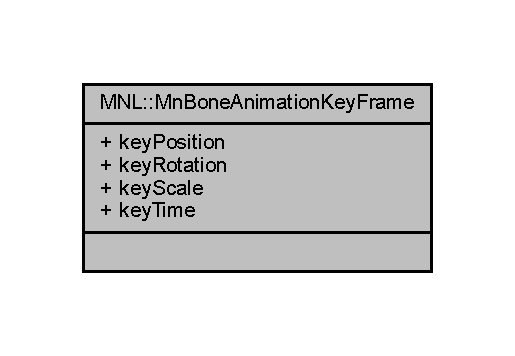
\includegraphics[width=247pt]{struct_m_n_l_1_1_mn_bone_animation_key_frame__coll__graph}
\end{center}
\end{figure}
\subsection*{Public 속성}
\begin{DoxyCompactItemize}
\item 
Direct\+X\+::\+Simple\+Math\+::\+Vector3 \hyperlink{struct_m_n_l_1_1_mn_bone_animation_key_frame_a322f5dacc90354870a569e3ad80d3ff6}{key\+Position}
\item 
Direct\+X\+::\+Simple\+Math\+::\+Quaternion \hyperlink{struct_m_n_l_1_1_mn_bone_animation_key_frame_a8ac33192c9eb7d8691540fceb3d0e1f9}{key\+Rotation}
\item 
Direct\+X\+::\+Simple\+Math\+::\+Vector3 \hyperlink{struct_m_n_l_1_1_mn_bone_animation_key_frame_ab79a35c4dfd72423eb6adff72d91e0c3}{key\+Scale}
\item 
double \hyperlink{struct_m_n_l_1_1_mn_bone_animation_key_frame_add992780bbdd3b047486ded8c0f8c953}{key\+Time}
\end{DoxyCompactItemize}


\subsection{상세한 설명}


Mn\+Bone\+Animation\+Element.\+h 파일의 10 번째 라인에서 정의되었습니다.



\subsection{멤버 데이터 문서화}
\mbox{\Hypertarget{struct_m_n_l_1_1_mn_bone_animation_key_frame_a322f5dacc90354870a569e3ad80d3ff6}\label{struct_m_n_l_1_1_mn_bone_animation_key_frame_a322f5dacc90354870a569e3ad80d3ff6}} 
\index{M\+N\+L\+::\+Mn\+Bone\+Animation\+Key\+Frame@{M\+N\+L\+::\+Mn\+Bone\+Animation\+Key\+Frame}!key\+Position@{key\+Position}}
\index{key\+Position@{key\+Position}!M\+N\+L\+::\+Mn\+Bone\+Animation\+Key\+Frame@{M\+N\+L\+::\+Mn\+Bone\+Animation\+Key\+Frame}}
\subsubsection{\texorpdfstring{key\+Position}{keyPosition}}
{\footnotesize\ttfamily Direct\+X\+::\+Simple\+Math\+::\+Vector3 M\+N\+L\+::\+Mn\+Bone\+Animation\+Key\+Frame\+::key\+Position}



Mn\+Bone\+Animation\+Element.\+h 파일의 12 번째 라인에서 정의되었습니다.

\mbox{\Hypertarget{struct_m_n_l_1_1_mn_bone_animation_key_frame_a8ac33192c9eb7d8691540fceb3d0e1f9}\label{struct_m_n_l_1_1_mn_bone_animation_key_frame_a8ac33192c9eb7d8691540fceb3d0e1f9}} 
\index{M\+N\+L\+::\+Mn\+Bone\+Animation\+Key\+Frame@{M\+N\+L\+::\+Mn\+Bone\+Animation\+Key\+Frame}!key\+Rotation@{key\+Rotation}}
\index{key\+Rotation@{key\+Rotation}!M\+N\+L\+::\+Mn\+Bone\+Animation\+Key\+Frame@{M\+N\+L\+::\+Mn\+Bone\+Animation\+Key\+Frame}}
\subsubsection{\texorpdfstring{key\+Rotation}{keyRotation}}
{\footnotesize\ttfamily Direct\+X\+::\+Simple\+Math\+::\+Quaternion M\+N\+L\+::\+Mn\+Bone\+Animation\+Key\+Frame\+::key\+Rotation}



Mn\+Bone\+Animation\+Element.\+h 파일의 13 번째 라인에서 정의되었습니다.

\mbox{\Hypertarget{struct_m_n_l_1_1_mn_bone_animation_key_frame_ab79a35c4dfd72423eb6adff72d91e0c3}\label{struct_m_n_l_1_1_mn_bone_animation_key_frame_ab79a35c4dfd72423eb6adff72d91e0c3}} 
\index{M\+N\+L\+::\+Mn\+Bone\+Animation\+Key\+Frame@{M\+N\+L\+::\+Mn\+Bone\+Animation\+Key\+Frame}!key\+Scale@{key\+Scale}}
\index{key\+Scale@{key\+Scale}!M\+N\+L\+::\+Mn\+Bone\+Animation\+Key\+Frame@{M\+N\+L\+::\+Mn\+Bone\+Animation\+Key\+Frame}}
\subsubsection{\texorpdfstring{key\+Scale}{keyScale}}
{\footnotesize\ttfamily Direct\+X\+::\+Simple\+Math\+::\+Vector3 M\+N\+L\+::\+Mn\+Bone\+Animation\+Key\+Frame\+::key\+Scale}



Mn\+Bone\+Animation\+Element.\+h 파일의 14 번째 라인에서 정의되었습니다.

\mbox{\Hypertarget{struct_m_n_l_1_1_mn_bone_animation_key_frame_add992780bbdd3b047486ded8c0f8c953}\label{struct_m_n_l_1_1_mn_bone_animation_key_frame_add992780bbdd3b047486ded8c0f8c953}} 
\index{M\+N\+L\+::\+Mn\+Bone\+Animation\+Key\+Frame@{M\+N\+L\+::\+Mn\+Bone\+Animation\+Key\+Frame}!key\+Time@{key\+Time}}
\index{key\+Time@{key\+Time}!M\+N\+L\+::\+Mn\+Bone\+Animation\+Key\+Frame@{M\+N\+L\+::\+Mn\+Bone\+Animation\+Key\+Frame}}
\subsubsection{\texorpdfstring{key\+Time}{keyTime}}
{\footnotesize\ttfamily double M\+N\+L\+::\+Mn\+Bone\+Animation\+Key\+Frame\+::key\+Time}



Mn\+Bone\+Animation\+Element.\+h 파일의 15 번째 라인에서 정의되었습니다.



이 구조체에 대한 문서화 페이지는 다음의 파일로부터 생성되었습니다.\+:\begin{DoxyCompactItemize}
\item 
Render/\hyperlink{_mn_bone_animation_element_8h}{Mn\+Bone\+Animation\+Element.\+h}\end{DoxyCompactItemize}

\hypertarget{class_m_n_l_1_1_mn_bone_animation_tracker}{}\section{M\+NL\+:\+:Mn\+Bone\+Animation\+Tracker 클래스 참조}
\label{class_m_n_l_1_1_mn_bone_animation_tracker}\index{M\+N\+L\+::\+Mn\+Bone\+Animation\+Tracker@{M\+N\+L\+::\+Mn\+Bone\+Animation\+Tracker}}


{\ttfamily \#include $<$Mn\+Bone\+Animation\+Tracker.\+h$>$}



M\+NL\+:\+:Mn\+Bone\+Animation\+Tracker에 대한 협력 다이어그램\+:\nopagebreak
\begin{figure}[H]
\begin{center}
\leavevmode
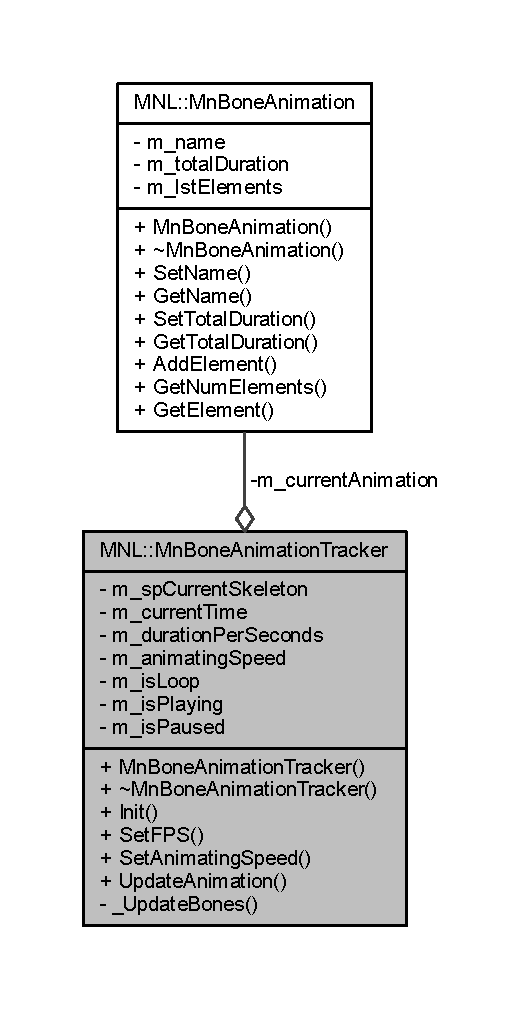
\includegraphics[width=252pt]{class_m_n_l_1_1_mn_bone_animation_tracker__coll__graph}
\end{center}
\end{figure}
\subsection*{Public 멤버 함수}
\begin{DoxyCompactItemize}
\item 
\hyperlink{class_m_n_l_1_1_mn_bone_animation_tracker_a54ca35d4c15067230ebcf72064abc319}{Mn\+Bone\+Animation\+Tracker} ()
\item 
\hyperlink{class_m_n_l_1_1_mn_bone_animation_tracker_a90ea134da8fbc89ed8f5d4b5b9e562fb}{$\sim$\+Mn\+Bone\+Animation\+Tracker} ()
\item 
H\+R\+E\+S\+U\+LT \hyperlink{class_m_n_l_1_1_mn_bone_animation_tracker_abe68ff29930c52db601b6158e5f03bf7}{Init} (const std\+::shared\+\_\+ptr$<$ \hyperlink{class_m_n_l_1_1_mn_skeleton}{Mn\+Skeleton} $>$ \&sp\+Skeleton, const \hyperlink{class_m_n_l_1_1_mn_bone_animation}{Mn\+Bone\+Animation} \&animation)
\item 
void \hyperlink{class_m_n_l_1_1_mn_bone_animation_tracker_a7e3a689e2850bc4cffec74444efd6129}{Set\+F\+PS} (double fps)
\item 
void \hyperlink{class_m_n_l_1_1_mn_bone_animation_tracker_a0bbded38ae7eb717880b49ed00b25f1f}{Set\+Animating\+Speed} (float speed)
\item 
void \hyperlink{class_m_n_l_1_1_mn_bone_animation_tracker_aa411090b4490d4c0422865ab8b563ddf}{Update\+Animation} (double time\+Delta)
\end{DoxyCompactItemize}
\subsection*{Private 멤버 함수}
\begin{DoxyCompactItemize}
\item 
void \hyperlink{class_m_n_l_1_1_mn_bone_animation_tracker_abb7e0010c3717fe7b6f54a6665b31bbc}{\+\_\+\+Update\+Bones} (float time\+Factor)
\end{DoxyCompactItemize}
\subsection*{Private 속성}
\begin{DoxyCompactItemize}
\item 
std\+::shared\+\_\+ptr$<$ \hyperlink{class_m_n_l_1_1_mn_skeleton}{Mn\+Skeleton} $>$ \hyperlink{class_m_n_l_1_1_mn_bone_animation_tracker_aefec935ed7824231963b657b8ddb914b}{m\+\_\+sp\+Current\+Skeleton}
\item 
\hyperlink{class_m_n_l_1_1_mn_bone_animation}{Mn\+Bone\+Animation} \hyperlink{class_m_n_l_1_1_mn_bone_animation_tracker_a8ce5bc87cbbfd5fbb8d442cceb7df2f5}{m\+\_\+current\+Animation}
\item 
double \hyperlink{class_m_n_l_1_1_mn_bone_animation_tracker_acf1032e7352339dbccc640681bb3895a}{m\+\_\+current\+Time}
\item 
double \hyperlink{class_m_n_l_1_1_mn_bone_animation_tracker_aecccf5c8a3fde50062469a35ea083d59}{m\+\_\+duration\+Per\+Seconds}
\item 
float \hyperlink{class_m_n_l_1_1_mn_bone_animation_tracker_aefbe185491262dba571d1201677ef7e1}{m\+\_\+animating\+Speed}
\item 
bool \hyperlink{class_m_n_l_1_1_mn_bone_animation_tracker_af52c92c8b507e21c94457ac47a5641bb}{m\+\_\+is\+Loop}
\item 
bool \hyperlink{class_m_n_l_1_1_mn_bone_animation_tracker_ac5dad518bde253882bda51dd30240d14}{m\+\_\+is\+Playing}
\item 
bool \hyperlink{class_m_n_l_1_1_mn_bone_animation_tracker_a8ed61397e39110735e5a400b78a42986}{m\+\_\+is\+Paused}
\end{DoxyCompactItemize}


\subsection{상세한 설명}


Mn\+Bone\+Animation\+Tracker.\+h 파일의 7 번째 라인에서 정의되었습니다.



\subsection{생성자 \& 소멸자 문서화}
\mbox{\Hypertarget{class_m_n_l_1_1_mn_bone_animation_tracker_a54ca35d4c15067230ebcf72064abc319}\label{class_m_n_l_1_1_mn_bone_animation_tracker_a54ca35d4c15067230ebcf72064abc319}} 
\index{M\+N\+L\+::\+Mn\+Bone\+Animation\+Tracker@{M\+N\+L\+::\+Mn\+Bone\+Animation\+Tracker}!Mn\+Bone\+Animation\+Tracker@{Mn\+Bone\+Animation\+Tracker}}
\index{Mn\+Bone\+Animation\+Tracker@{Mn\+Bone\+Animation\+Tracker}!M\+N\+L\+::\+Mn\+Bone\+Animation\+Tracker@{M\+N\+L\+::\+Mn\+Bone\+Animation\+Tracker}}
\subsubsection{\texorpdfstring{Mn\+Bone\+Animation\+Tracker()}{MnBoneAnimationTracker()}}
{\footnotesize\ttfamily Mn\+Bone\+Animation\+Tracker\+::\+Mn\+Bone\+Animation\+Tracker (\begin{DoxyParamCaption}{ }\end{DoxyParamCaption})}



Mn\+Bone\+Animation\+Tracker.\+cpp 파일의 6 번째 라인에서 정의되었습니다.

\mbox{\Hypertarget{class_m_n_l_1_1_mn_bone_animation_tracker_a90ea134da8fbc89ed8f5d4b5b9e562fb}\label{class_m_n_l_1_1_mn_bone_animation_tracker_a90ea134da8fbc89ed8f5d4b5b9e562fb}} 
\index{M\+N\+L\+::\+Mn\+Bone\+Animation\+Tracker@{M\+N\+L\+::\+Mn\+Bone\+Animation\+Tracker}!````~Mn\+Bone\+Animation\+Tracker@{$\sim$\+Mn\+Bone\+Animation\+Tracker}}
\index{````~Mn\+Bone\+Animation\+Tracker@{$\sim$\+Mn\+Bone\+Animation\+Tracker}!M\+N\+L\+::\+Mn\+Bone\+Animation\+Tracker@{M\+N\+L\+::\+Mn\+Bone\+Animation\+Tracker}}
\subsubsection{\texorpdfstring{$\sim$\+Mn\+Bone\+Animation\+Tracker()}{~MnBoneAnimationTracker()}}
{\footnotesize\ttfamily Mn\+Bone\+Animation\+Tracker\+::$\sim$\+Mn\+Bone\+Animation\+Tracker (\begin{DoxyParamCaption}{ }\end{DoxyParamCaption})}



Mn\+Bone\+Animation\+Tracker.\+cpp 파일의 16 번째 라인에서 정의되었습니다.



\subsection{멤버 함수 문서화}
\mbox{\Hypertarget{class_m_n_l_1_1_mn_bone_animation_tracker_abb7e0010c3717fe7b6f54a6665b31bbc}\label{class_m_n_l_1_1_mn_bone_animation_tracker_abb7e0010c3717fe7b6f54a6665b31bbc}} 
\index{M\+N\+L\+::\+Mn\+Bone\+Animation\+Tracker@{M\+N\+L\+::\+Mn\+Bone\+Animation\+Tracker}!\+\_\+\+Update\+Bones@{\+\_\+\+Update\+Bones}}
\index{\+\_\+\+Update\+Bones@{\+\_\+\+Update\+Bones}!M\+N\+L\+::\+Mn\+Bone\+Animation\+Tracker@{M\+N\+L\+::\+Mn\+Bone\+Animation\+Tracker}}
\subsubsection{\texorpdfstring{\+\_\+\+Update\+Bones()}{\_UpdateBones()}}
{\footnotesize\ttfamily void Mn\+Bone\+Animation\+Tracker\+::\+\_\+\+Update\+Bones (\begin{DoxyParamCaption}\item[{float}]{time\+Factor }\end{DoxyParamCaption})\hspace{0.3cm}{\ttfamily [private]}}



Mn\+Bone\+Animation\+Tracker.\+cpp 파일의 51 번째 라인에서 정의되었습니다.

\mbox{\Hypertarget{class_m_n_l_1_1_mn_bone_animation_tracker_abe68ff29930c52db601b6158e5f03bf7}\label{class_m_n_l_1_1_mn_bone_animation_tracker_abe68ff29930c52db601b6158e5f03bf7}} 
\index{M\+N\+L\+::\+Mn\+Bone\+Animation\+Tracker@{M\+N\+L\+::\+Mn\+Bone\+Animation\+Tracker}!Init@{Init}}
\index{Init@{Init}!M\+N\+L\+::\+Mn\+Bone\+Animation\+Tracker@{M\+N\+L\+::\+Mn\+Bone\+Animation\+Tracker}}
\subsubsection{\texorpdfstring{Init()}{Init()}}
{\footnotesize\ttfamily H\+R\+E\+S\+U\+LT Mn\+Bone\+Animation\+Tracker\+::\+Init (\begin{DoxyParamCaption}\item[{const std\+::shared\+\_\+ptr$<$ \hyperlink{class_m_n_l_1_1_mn_skeleton}{Mn\+Skeleton} $>$ \&}]{sp\+Skeleton,  }\item[{const \hyperlink{class_m_n_l_1_1_mn_bone_animation}{Mn\+Bone\+Animation} \&}]{animation }\end{DoxyParamCaption})}



Mn\+Bone\+Animation\+Tracker.\+cpp 파일의 20 번째 라인에서 정의되었습니다.

\mbox{\Hypertarget{class_m_n_l_1_1_mn_bone_animation_tracker_a0bbded38ae7eb717880b49ed00b25f1f}\label{class_m_n_l_1_1_mn_bone_animation_tracker_a0bbded38ae7eb717880b49ed00b25f1f}} 
\index{M\+N\+L\+::\+Mn\+Bone\+Animation\+Tracker@{M\+N\+L\+::\+Mn\+Bone\+Animation\+Tracker}!Set\+Animating\+Speed@{Set\+Animating\+Speed}}
\index{Set\+Animating\+Speed@{Set\+Animating\+Speed}!M\+N\+L\+::\+Mn\+Bone\+Animation\+Tracker@{M\+N\+L\+::\+Mn\+Bone\+Animation\+Tracker}}
\subsubsection{\texorpdfstring{Set\+Animating\+Speed()}{SetAnimatingSpeed()}}
{\footnotesize\ttfamily void Mn\+Bone\+Animation\+Tracker\+::\+Set\+Animating\+Speed (\begin{DoxyParamCaption}\item[{float}]{speed }\end{DoxyParamCaption})}



Mn\+Bone\+Animation\+Tracker.\+cpp 파일의 31 번째 라인에서 정의되었습니다.

\mbox{\Hypertarget{class_m_n_l_1_1_mn_bone_animation_tracker_a7e3a689e2850bc4cffec74444efd6129}\label{class_m_n_l_1_1_mn_bone_animation_tracker_a7e3a689e2850bc4cffec74444efd6129}} 
\index{M\+N\+L\+::\+Mn\+Bone\+Animation\+Tracker@{M\+N\+L\+::\+Mn\+Bone\+Animation\+Tracker}!Set\+F\+PS@{Set\+F\+PS}}
\index{Set\+F\+PS@{Set\+F\+PS}!M\+N\+L\+::\+Mn\+Bone\+Animation\+Tracker@{M\+N\+L\+::\+Mn\+Bone\+Animation\+Tracker}}
\subsubsection{\texorpdfstring{Set\+F\+P\+S()}{SetFPS()}}
{\footnotesize\ttfamily void Mn\+Bone\+Animation\+Tracker\+::\+Set\+F\+PS (\begin{DoxyParamCaption}\item[{double}]{fps }\end{DoxyParamCaption})}



Mn\+Bone\+Animation\+Tracker.\+cpp 파일의 27 번째 라인에서 정의되었습니다.

\mbox{\Hypertarget{class_m_n_l_1_1_mn_bone_animation_tracker_aa411090b4490d4c0422865ab8b563ddf}\label{class_m_n_l_1_1_mn_bone_animation_tracker_aa411090b4490d4c0422865ab8b563ddf}} 
\index{M\+N\+L\+::\+Mn\+Bone\+Animation\+Tracker@{M\+N\+L\+::\+Mn\+Bone\+Animation\+Tracker}!Update\+Animation@{Update\+Animation}}
\index{Update\+Animation@{Update\+Animation}!M\+N\+L\+::\+Mn\+Bone\+Animation\+Tracker@{M\+N\+L\+::\+Mn\+Bone\+Animation\+Tracker}}
\subsubsection{\texorpdfstring{Update\+Animation()}{UpdateAnimation()}}
{\footnotesize\ttfamily void Mn\+Bone\+Animation\+Tracker\+::\+Update\+Animation (\begin{DoxyParamCaption}\item[{double}]{time\+Delta }\end{DoxyParamCaption})}



Mn\+Bone\+Animation\+Tracker.\+cpp 파일의 38 번째 라인에서 정의되었습니다.



\subsection{멤버 데이터 문서화}
\mbox{\Hypertarget{class_m_n_l_1_1_mn_bone_animation_tracker_aefbe185491262dba571d1201677ef7e1}\label{class_m_n_l_1_1_mn_bone_animation_tracker_aefbe185491262dba571d1201677ef7e1}} 
\index{M\+N\+L\+::\+Mn\+Bone\+Animation\+Tracker@{M\+N\+L\+::\+Mn\+Bone\+Animation\+Tracker}!m\+\_\+animating\+Speed@{m\+\_\+animating\+Speed}}
\index{m\+\_\+animating\+Speed@{m\+\_\+animating\+Speed}!M\+N\+L\+::\+Mn\+Bone\+Animation\+Tracker@{M\+N\+L\+::\+Mn\+Bone\+Animation\+Tracker}}
\subsubsection{\texorpdfstring{m\+\_\+animating\+Speed}{m\_animatingSpeed}}
{\footnotesize\ttfamily float M\+N\+L\+::\+Mn\+Bone\+Animation\+Tracker\+::m\+\_\+animating\+Speed\hspace{0.3cm}{\ttfamily [private]}}



Mn\+Bone\+Animation\+Tracker.\+h 파일의 40 번째 라인에서 정의되었습니다.

\mbox{\Hypertarget{class_m_n_l_1_1_mn_bone_animation_tracker_a8ce5bc87cbbfd5fbb8d442cceb7df2f5}\label{class_m_n_l_1_1_mn_bone_animation_tracker_a8ce5bc87cbbfd5fbb8d442cceb7df2f5}} 
\index{M\+N\+L\+::\+Mn\+Bone\+Animation\+Tracker@{M\+N\+L\+::\+Mn\+Bone\+Animation\+Tracker}!m\+\_\+current\+Animation@{m\+\_\+current\+Animation}}
\index{m\+\_\+current\+Animation@{m\+\_\+current\+Animation}!M\+N\+L\+::\+Mn\+Bone\+Animation\+Tracker@{M\+N\+L\+::\+Mn\+Bone\+Animation\+Tracker}}
\subsubsection{\texorpdfstring{m\+\_\+current\+Animation}{m\_currentAnimation}}
{\footnotesize\ttfamily \hyperlink{class_m_n_l_1_1_mn_bone_animation}{Mn\+Bone\+Animation} M\+N\+L\+::\+Mn\+Bone\+Animation\+Tracker\+::m\+\_\+current\+Animation\hspace{0.3cm}{\ttfamily [private]}}



Mn\+Bone\+Animation\+Tracker.\+h 파일의 31 번째 라인에서 정의되었습니다.

\mbox{\Hypertarget{class_m_n_l_1_1_mn_bone_animation_tracker_acf1032e7352339dbccc640681bb3895a}\label{class_m_n_l_1_1_mn_bone_animation_tracker_acf1032e7352339dbccc640681bb3895a}} 
\index{M\+N\+L\+::\+Mn\+Bone\+Animation\+Tracker@{M\+N\+L\+::\+Mn\+Bone\+Animation\+Tracker}!m\+\_\+current\+Time@{m\+\_\+current\+Time}}
\index{m\+\_\+current\+Time@{m\+\_\+current\+Time}!M\+N\+L\+::\+Mn\+Bone\+Animation\+Tracker@{M\+N\+L\+::\+Mn\+Bone\+Animation\+Tracker}}
\subsubsection{\texorpdfstring{m\+\_\+current\+Time}{m\_currentTime}}
{\footnotesize\ttfamily double M\+N\+L\+::\+Mn\+Bone\+Animation\+Tracker\+::m\+\_\+current\+Time\hspace{0.3cm}{\ttfamily [private]}}



Mn\+Bone\+Animation\+Tracker.\+h 파일의 32 번째 라인에서 정의되었습니다.

\mbox{\Hypertarget{class_m_n_l_1_1_mn_bone_animation_tracker_aecccf5c8a3fde50062469a35ea083d59}\label{class_m_n_l_1_1_mn_bone_animation_tracker_aecccf5c8a3fde50062469a35ea083d59}} 
\index{M\+N\+L\+::\+Mn\+Bone\+Animation\+Tracker@{M\+N\+L\+::\+Mn\+Bone\+Animation\+Tracker}!m\+\_\+duration\+Per\+Seconds@{m\+\_\+duration\+Per\+Seconds}}
\index{m\+\_\+duration\+Per\+Seconds@{m\+\_\+duration\+Per\+Seconds}!M\+N\+L\+::\+Mn\+Bone\+Animation\+Tracker@{M\+N\+L\+::\+Mn\+Bone\+Animation\+Tracker}}
\subsubsection{\texorpdfstring{m\+\_\+duration\+Per\+Seconds}{m\_durationPerSeconds}}
{\footnotesize\ttfamily double M\+N\+L\+::\+Mn\+Bone\+Animation\+Tracker\+::m\+\_\+duration\+Per\+Seconds\hspace{0.3cm}{\ttfamily [private]}}



Mn\+Bone\+Animation\+Tracker.\+h 파일의 36 번째 라인에서 정의되었습니다.

\mbox{\Hypertarget{class_m_n_l_1_1_mn_bone_animation_tracker_af52c92c8b507e21c94457ac47a5641bb}\label{class_m_n_l_1_1_mn_bone_animation_tracker_af52c92c8b507e21c94457ac47a5641bb}} 
\index{M\+N\+L\+::\+Mn\+Bone\+Animation\+Tracker@{M\+N\+L\+::\+Mn\+Bone\+Animation\+Tracker}!m\+\_\+is\+Loop@{m\+\_\+is\+Loop}}
\index{m\+\_\+is\+Loop@{m\+\_\+is\+Loop}!M\+N\+L\+::\+Mn\+Bone\+Animation\+Tracker@{M\+N\+L\+::\+Mn\+Bone\+Animation\+Tracker}}
\subsubsection{\texorpdfstring{m\+\_\+is\+Loop}{m\_isLoop}}
{\footnotesize\ttfamily bool M\+N\+L\+::\+Mn\+Bone\+Animation\+Tracker\+::m\+\_\+is\+Loop\hspace{0.3cm}{\ttfamily [private]}}



Mn\+Bone\+Animation\+Tracker.\+h 파일의 42 번째 라인에서 정의되었습니다.

\mbox{\Hypertarget{class_m_n_l_1_1_mn_bone_animation_tracker_a8ed61397e39110735e5a400b78a42986}\label{class_m_n_l_1_1_mn_bone_animation_tracker_a8ed61397e39110735e5a400b78a42986}} 
\index{M\+N\+L\+::\+Mn\+Bone\+Animation\+Tracker@{M\+N\+L\+::\+Mn\+Bone\+Animation\+Tracker}!m\+\_\+is\+Paused@{m\+\_\+is\+Paused}}
\index{m\+\_\+is\+Paused@{m\+\_\+is\+Paused}!M\+N\+L\+::\+Mn\+Bone\+Animation\+Tracker@{M\+N\+L\+::\+Mn\+Bone\+Animation\+Tracker}}
\subsubsection{\texorpdfstring{m\+\_\+is\+Paused}{m\_isPaused}}
{\footnotesize\ttfamily bool M\+N\+L\+::\+Mn\+Bone\+Animation\+Tracker\+::m\+\_\+is\+Paused\hspace{0.3cm}{\ttfamily [private]}}



Mn\+Bone\+Animation\+Tracker.\+h 파일의 44 번째 라인에서 정의되었습니다.

\mbox{\Hypertarget{class_m_n_l_1_1_mn_bone_animation_tracker_ac5dad518bde253882bda51dd30240d14}\label{class_m_n_l_1_1_mn_bone_animation_tracker_ac5dad518bde253882bda51dd30240d14}} 
\index{M\+N\+L\+::\+Mn\+Bone\+Animation\+Tracker@{M\+N\+L\+::\+Mn\+Bone\+Animation\+Tracker}!m\+\_\+is\+Playing@{m\+\_\+is\+Playing}}
\index{m\+\_\+is\+Playing@{m\+\_\+is\+Playing}!M\+N\+L\+::\+Mn\+Bone\+Animation\+Tracker@{M\+N\+L\+::\+Mn\+Bone\+Animation\+Tracker}}
\subsubsection{\texorpdfstring{m\+\_\+is\+Playing}{m\_isPlaying}}
{\footnotesize\ttfamily bool M\+N\+L\+::\+Mn\+Bone\+Animation\+Tracker\+::m\+\_\+is\+Playing\hspace{0.3cm}{\ttfamily [private]}}



Mn\+Bone\+Animation\+Tracker.\+h 파일의 43 번째 라인에서 정의되었습니다.

\mbox{\Hypertarget{class_m_n_l_1_1_mn_bone_animation_tracker_aefec935ed7824231963b657b8ddb914b}\label{class_m_n_l_1_1_mn_bone_animation_tracker_aefec935ed7824231963b657b8ddb914b}} 
\index{M\+N\+L\+::\+Mn\+Bone\+Animation\+Tracker@{M\+N\+L\+::\+Mn\+Bone\+Animation\+Tracker}!m\+\_\+sp\+Current\+Skeleton@{m\+\_\+sp\+Current\+Skeleton}}
\index{m\+\_\+sp\+Current\+Skeleton@{m\+\_\+sp\+Current\+Skeleton}!M\+N\+L\+::\+Mn\+Bone\+Animation\+Tracker@{M\+N\+L\+::\+Mn\+Bone\+Animation\+Tracker}}
\subsubsection{\texorpdfstring{m\+\_\+sp\+Current\+Skeleton}{m\_spCurrentSkeleton}}
{\footnotesize\ttfamily std\+::shared\+\_\+ptr$<$\hyperlink{class_m_n_l_1_1_mn_skeleton}{Mn\+Skeleton}$>$ M\+N\+L\+::\+Mn\+Bone\+Animation\+Tracker\+::m\+\_\+sp\+Current\+Skeleton\hspace{0.3cm}{\ttfamily [private]}}



Mn\+Bone\+Animation\+Tracker.\+h 파일의 30 번째 라인에서 정의되었습니다.



이 클래스에 대한 문서화 페이지는 다음의 파일들로부터 생성되었습니다.\+:\begin{DoxyCompactItemize}
\item 
Render/\hyperlink{_mn_bone_animation_tracker_8h}{Mn\+Bone\+Animation\+Tracker.\+h}\item 
Render/\hyperlink{_mn_bone_animation_tracker_8cpp}{Mn\+Bone\+Animation\+Tracker.\+cpp}\end{DoxyCompactItemize}

\hypertarget{class_m_n_l_1_1_mn_camera}{}\section{M\+NL\+:\+:Mn\+Camera 클래스 참조}
\label{class_m_n_l_1_1_mn_camera}\index{M\+N\+L\+::\+Mn\+Camera@{M\+N\+L\+::\+Mn\+Camera}}


{\ttfamily \#include $<$Mn\+Camera.\+h$>$}



M\+NL\+:\+:Mn\+Camera에 대한 협력 다이어그램\+:\nopagebreak
\begin{figure}[H]
\begin{center}
\leavevmode
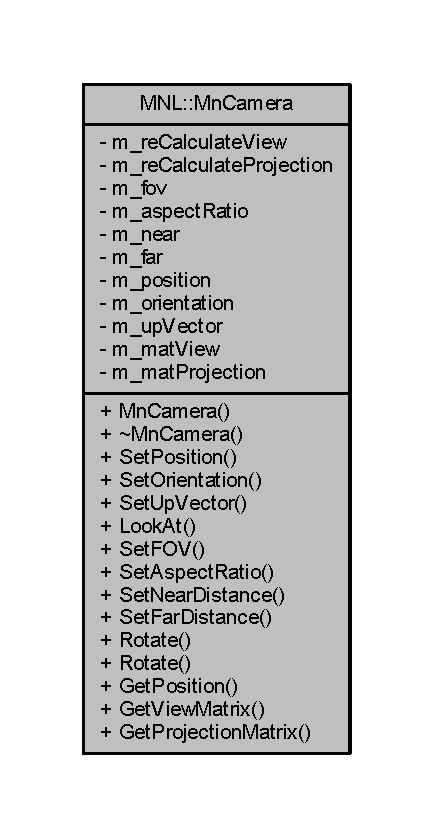
\includegraphics[width=208pt]{class_m_n_l_1_1_mn_camera__coll__graph}
\end{center}
\end{figure}
\subsection*{Public 멤버 함수}
\begin{DoxyCompactItemize}
\item 
\hyperlink{class_m_n_l_1_1_mn_camera_aff0b3d9da025157410805fc0c2e3659f}{Mn\+Camera} ()
\item 
\hyperlink{class_m_n_l_1_1_mn_camera_aebde880f88a052f4e7133de9de74509e}{$\sim$\+Mn\+Camera} ()
\item 
void \hyperlink{class_m_n_l_1_1_mn_camera_ab15d02ee68e0588a96a0c44ac486cd18}{Set\+Position} (const Direct\+X\+::\+Simple\+Math\+::\+Vector3 \&position)
\item 
void \hyperlink{class_m_n_l_1_1_mn_camera_ad9d9cc078cdeda1d5a8ef138a063c46f}{Set\+Orientation} (const Direct\+X\+::\+Simple\+Math\+::\+Vector3 \&orientation)
\item 
void \hyperlink{class_m_n_l_1_1_mn_camera_af287f66d56ecb6eba46efd12542e5cc6}{Set\+Up\+Vector} (const Direct\+X\+::\+Simple\+Math\+::\+Vector3 \&up\+Vec)
\item 
void \hyperlink{class_m_n_l_1_1_mn_camera_ad7fb1372db13a5ce955000a9597a9d48}{Look\+At} (const Direct\+X\+::\+Simple\+Math\+::\+Vector3 \&target, const Direct\+X\+::\+Simple\+Math\+::\+Vector3 \&up\+Vec)
\item 
void \hyperlink{class_m_n_l_1_1_mn_camera_a624327e866968d1df7fb73d2019d6aab}{Set\+F\+OV} (float rad\+F\+OV)
\item 
void \hyperlink{class_m_n_l_1_1_mn_camera_ac506b6bd606f8716e3dff87e80def299}{Set\+Aspect\+Ratio} (float aspect\+Ratio)
\item 
void \hyperlink{class_m_n_l_1_1_mn_camera_adb743c4f0499bc4b4346d39c1739cdb3}{Set\+Near\+Distance} (float near)
\item 
void \hyperlink{class_m_n_l_1_1_mn_camera_ab7c4cbd91462c20e32ac2b80aa83474c}{Set\+Far\+Distance} (float far)
\item 
void \hyperlink{class_m_n_l_1_1_mn_camera_a0e0d866c3cacedbceceed4dddaa0b473}{Rotate} (const Direct\+X\+::\+Simple\+Math\+::\+Quaternion \&quat)
\item 
void \hyperlink{class_m_n_l_1_1_mn_camera_ad6e912e0b1bae0cef9c41edeeb1a79da}{Rotate} (const Direct\+X\+::\+Simple\+Math\+::\+Vector3 \&axis, float rad)
\item 
const Direct\+X\+::\+Simple\+Math\+::\+Vector3 \& \hyperlink{class_m_n_l_1_1_mn_camera_a478d9bd34d90ae8bb06cdbb4193d48b7}{Get\+Position} () const
\item 
const Direct\+X\+::\+Simple\+Math\+::\+Matrix \& \hyperlink{class_m_n_l_1_1_mn_camera_a5b4d56e3d1d459da5c346831b1e43510}{Get\+View\+Matrix} ()
\item 
const Direct\+X\+::\+Simple\+Math\+::\+Matrix \& \hyperlink{class_m_n_l_1_1_mn_camera_a7b8773bec079b174185732f80e32d943}{Get\+Projection\+Matrix} ()
\end{DoxyCompactItemize}
\subsection*{Private 속성}
\begin{DoxyCompactItemize}
\item 
bool \hyperlink{class_m_n_l_1_1_mn_camera_a84a4810d902a48aa0b123bdd0dc5e6f5}{m\+\_\+re\+Calculate\+View}
\item 
bool \hyperlink{class_m_n_l_1_1_mn_camera_abad8116c842d5680d3c545aa20452cbe}{m\+\_\+re\+Calculate\+Projection}
\item 
float \hyperlink{class_m_n_l_1_1_mn_camera_a953e98334e299bb5231c12725426e9e1}{m\+\_\+fov}
\item 
float \hyperlink{class_m_n_l_1_1_mn_camera_a8b651cf5f971172916403ea79c0a553f}{m\+\_\+aspect\+Ratio}
\item 
float \hyperlink{class_m_n_l_1_1_mn_camera_a91e640f0f4ca4c834d1412befcbc54c2}{m\+\_\+near}
\item 
float \hyperlink{class_m_n_l_1_1_mn_camera_aba7e7ba5a457118a27f51b4e1d215e6d}{m\+\_\+far}
\item 
Direct\+X\+::\+Simple\+Math\+::\+Vector3 \hyperlink{class_m_n_l_1_1_mn_camera_aea21f690e7007b7ea8b4c2348e81e421}{m\+\_\+position}
\item 
Direct\+X\+::\+Simple\+Math\+::\+Vector3 \hyperlink{class_m_n_l_1_1_mn_camera_a329c94f5c273c0d53522663678889f1e}{m\+\_\+orientation}
\item 
Direct\+X\+::\+Simple\+Math\+::\+Vector3 \hyperlink{class_m_n_l_1_1_mn_camera_ab1138f925c50ceea63bf0d510d8df0d0}{m\+\_\+up\+Vector}
\item 
Direct\+X\+::\+Simple\+Math\+::\+Matrix \hyperlink{class_m_n_l_1_1_mn_camera_ac4717e21e16d9d3007e788fbe2e299de}{m\+\_\+mat\+View}
\item 
Direct\+X\+::\+Simple\+Math\+::\+Matrix \hyperlink{class_m_n_l_1_1_mn_camera_a2fe67aae96095cd1c54ab1e9f71e06f7}{m\+\_\+mat\+Projection}
\end{DoxyCompactItemize}


\subsection{상세한 설명}


Mn\+Camera.\+h 파일의 7 번째 라인에서 정의되었습니다.



\subsection{생성자 \& 소멸자 문서화}
\mbox{\Hypertarget{class_m_n_l_1_1_mn_camera_aff0b3d9da025157410805fc0c2e3659f}\label{class_m_n_l_1_1_mn_camera_aff0b3d9da025157410805fc0c2e3659f}} 
\index{M\+N\+L\+::\+Mn\+Camera@{M\+N\+L\+::\+Mn\+Camera}!Mn\+Camera@{Mn\+Camera}}
\index{Mn\+Camera@{Mn\+Camera}!M\+N\+L\+::\+Mn\+Camera@{M\+N\+L\+::\+Mn\+Camera}}
\subsubsection{\texorpdfstring{Mn\+Camera()}{MnCamera()}}
{\footnotesize\ttfamily Mn\+Camera\+::\+Mn\+Camera (\begin{DoxyParamCaption}{ }\end{DoxyParamCaption})}



Mn\+Camera.\+cpp 파일의 6 번째 라인에서 정의되었습니다.

\mbox{\Hypertarget{class_m_n_l_1_1_mn_camera_aebde880f88a052f4e7133de9de74509e}\label{class_m_n_l_1_1_mn_camera_aebde880f88a052f4e7133de9de74509e}} 
\index{M\+N\+L\+::\+Mn\+Camera@{M\+N\+L\+::\+Mn\+Camera}!````~Mn\+Camera@{$\sim$\+Mn\+Camera}}
\index{````~Mn\+Camera@{$\sim$\+Mn\+Camera}!M\+N\+L\+::\+Mn\+Camera@{M\+N\+L\+::\+Mn\+Camera}}
\subsubsection{\texorpdfstring{$\sim$\+Mn\+Camera()}{~MnCamera()}}
{\footnotesize\ttfamily Mn\+Camera\+::$\sim$\+Mn\+Camera (\begin{DoxyParamCaption}{ }\end{DoxyParamCaption})}



Mn\+Camera.\+cpp 파일의 16 번째 라인에서 정의되었습니다.



\subsection{멤버 함수 문서화}
\mbox{\Hypertarget{class_m_n_l_1_1_mn_camera_a478d9bd34d90ae8bb06cdbb4193d48b7}\label{class_m_n_l_1_1_mn_camera_a478d9bd34d90ae8bb06cdbb4193d48b7}} 
\index{M\+N\+L\+::\+Mn\+Camera@{M\+N\+L\+::\+Mn\+Camera}!Get\+Position@{Get\+Position}}
\index{Get\+Position@{Get\+Position}!M\+N\+L\+::\+Mn\+Camera@{M\+N\+L\+::\+Mn\+Camera}}
\subsubsection{\texorpdfstring{Get\+Position()}{GetPosition()}}
{\footnotesize\ttfamily const Direct\+X\+::\+Simple\+Math\+::\+Vector3 \& Mn\+Camera\+::\+Get\+Position (\begin{DoxyParamCaption}{ }\end{DoxyParamCaption}) const}



Mn\+Camera.\+cpp 파일의 72 번째 라인에서 정의되었습니다.

\mbox{\Hypertarget{class_m_n_l_1_1_mn_camera_a7b8773bec079b174185732f80e32d943}\label{class_m_n_l_1_1_mn_camera_a7b8773bec079b174185732f80e32d943}} 
\index{M\+N\+L\+::\+Mn\+Camera@{M\+N\+L\+::\+Mn\+Camera}!Get\+Projection\+Matrix@{Get\+Projection\+Matrix}}
\index{Get\+Projection\+Matrix@{Get\+Projection\+Matrix}!M\+N\+L\+::\+Mn\+Camera@{M\+N\+L\+::\+Mn\+Camera}}
\subsubsection{\texorpdfstring{Get\+Projection\+Matrix()}{GetProjectionMatrix()}}
{\footnotesize\ttfamily const Direct\+X\+::\+Simple\+Math\+::\+Matrix \& Mn\+Camera\+::\+Get\+Projection\+Matrix (\begin{DoxyParamCaption}{ }\end{DoxyParamCaption})}



Mn\+Camera.\+cpp 파일의 87 번째 라인에서 정의되었습니다.

\mbox{\Hypertarget{class_m_n_l_1_1_mn_camera_a5b4d56e3d1d459da5c346831b1e43510}\label{class_m_n_l_1_1_mn_camera_a5b4d56e3d1d459da5c346831b1e43510}} 
\index{M\+N\+L\+::\+Mn\+Camera@{M\+N\+L\+::\+Mn\+Camera}!Get\+View\+Matrix@{Get\+View\+Matrix}}
\index{Get\+View\+Matrix@{Get\+View\+Matrix}!M\+N\+L\+::\+Mn\+Camera@{M\+N\+L\+::\+Mn\+Camera}}
\subsubsection{\texorpdfstring{Get\+View\+Matrix()}{GetViewMatrix()}}
{\footnotesize\ttfamily const Direct\+X\+::\+Simple\+Math\+::\+Matrix \& Mn\+Camera\+::\+Get\+View\+Matrix (\begin{DoxyParamCaption}{ }\end{DoxyParamCaption})}



Mn\+Camera.\+cpp 파일의 76 번째 라인에서 정의되었습니다.

\mbox{\Hypertarget{class_m_n_l_1_1_mn_camera_ad7fb1372db13a5ce955000a9597a9d48}\label{class_m_n_l_1_1_mn_camera_ad7fb1372db13a5ce955000a9597a9d48}} 
\index{M\+N\+L\+::\+Mn\+Camera@{M\+N\+L\+::\+Mn\+Camera}!Look\+At@{Look\+At}}
\index{Look\+At@{Look\+At}!M\+N\+L\+::\+Mn\+Camera@{M\+N\+L\+::\+Mn\+Camera}}
\subsubsection{\texorpdfstring{Look\+At()}{LookAt()}}
{\footnotesize\ttfamily void Mn\+Camera\+::\+Look\+At (\begin{DoxyParamCaption}\item[{const Direct\+X\+::\+Simple\+Math\+::\+Vector3 \&}]{target,  }\item[{const Direct\+X\+::\+Simple\+Math\+::\+Vector3 \&}]{up\+Vec }\end{DoxyParamCaption})}



Mn\+Camera.\+cpp 파일의 34 번째 라인에서 정의되었습니다.

\mbox{\Hypertarget{class_m_n_l_1_1_mn_camera_a0e0d866c3cacedbceceed4dddaa0b473}\label{class_m_n_l_1_1_mn_camera_a0e0d866c3cacedbceceed4dddaa0b473}} 
\index{M\+N\+L\+::\+Mn\+Camera@{M\+N\+L\+::\+Mn\+Camera}!Rotate@{Rotate}}
\index{Rotate@{Rotate}!M\+N\+L\+::\+Mn\+Camera@{M\+N\+L\+::\+Mn\+Camera}}
\subsubsection{\texorpdfstring{Rotate()}{Rotate()}\hspace{0.1cm}{\footnotesize\ttfamily [1/2]}}
{\footnotesize\ttfamily void Mn\+Camera\+::\+Rotate (\begin{DoxyParamCaption}\item[{const Direct\+X\+::\+Simple\+Math\+::\+Quaternion \&}]{quat }\end{DoxyParamCaption})}



Mn\+Camera.\+cpp 파일의 61 번째 라인에서 정의되었습니다.

\mbox{\Hypertarget{class_m_n_l_1_1_mn_camera_ad6e912e0b1bae0cef9c41edeeb1a79da}\label{class_m_n_l_1_1_mn_camera_ad6e912e0b1bae0cef9c41edeeb1a79da}} 
\index{M\+N\+L\+::\+Mn\+Camera@{M\+N\+L\+::\+Mn\+Camera}!Rotate@{Rotate}}
\index{Rotate@{Rotate}!M\+N\+L\+::\+Mn\+Camera@{M\+N\+L\+::\+Mn\+Camera}}
\subsubsection{\texorpdfstring{Rotate()}{Rotate()}\hspace{0.1cm}{\footnotesize\ttfamily [2/2]}}
{\footnotesize\ttfamily void Mn\+Camera\+::\+Rotate (\begin{DoxyParamCaption}\item[{const Direct\+X\+::\+Simple\+Math\+::\+Vector3 \&}]{axis,  }\item[{float}]{rad }\end{DoxyParamCaption})}



Mn\+Camera.\+cpp 파일의 66 번째 라인에서 정의되었습니다.

\mbox{\Hypertarget{class_m_n_l_1_1_mn_camera_ac506b6bd606f8716e3dff87e80def299}\label{class_m_n_l_1_1_mn_camera_ac506b6bd606f8716e3dff87e80def299}} 
\index{M\+N\+L\+::\+Mn\+Camera@{M\+N\+L\+::\+Mn\+Camera}!Set\+Aspect\+Ratio@{Set\+Aspect\+Ratio}}
\index{Set\+Aspect\+Ratio@{Set\+Aspect\+Ratio}!M\+N\+L\+::\+Mn\+Camera@{M\+N\+L\+::\+Mn\+Camera}}
\subsubsection{\texorpdfstring{Set\+Aspect\+Ratio()}{SetAspectRatio()}}
{\footnotesize\ttfamily void Mn\+Camera\+::\+Set\+Aspect\+Ratio (\begin{DoxyParamCaption}\item[{float}]{aspect\+Ratio }\end{DoxyParamCaption})}



Mn\+Camera.\+cpp 파일의 45 번째 라인에서 정의되었습니다.

\mbox{\Hypertarget{class_m_n_l_1_1_mn_camera_ab7c4cbd91462c20e32ac2b80aa83474c}\label{class_m_n_l_1_1_mn_camera_ab7c4cbd91462c20e32ac2b80aa83474c}} 
\index{M\+N\+L\+::\+Mn\+Camera@{M\+N\+L\+::\+Mn\+Camera}!Set\+Far\+Distance@{Set\+Far\+Distance}}
\index{Set\+Far\+Distance@{Set\+Far\+Distance}!M\+N\+L\+::\+Mn\+Camera@{M\+N\+L\+::\+Mn\+Camera}}
\subsubsection{\texorpdfstring{Set\+Far\+Distance()}{SetFarDistance()}}
{\footnotesize\ttfamily void Mn\+Camera\+::\+Set\+Far\+Distance (\begin{DoxyParamCaption}\item[{float}]{far }\end{DoxyParamCaption})}



Mn\+Camera.\+cpp 파일의 55 번째 라인에서 정의되었습니다.

\mbox{\Hypertarget{class_m_n_l_1_1_mn_camera_a624327e866968d1df7fb73d2019d6aab}\label{class_m_n_l_1_1_mn_camera_a624327e866968d1df7fb73d2019d6aab}} 
\index{M\+N\+L\+::\+Mn\+Camera@{M\+N\+L\+::\+Mn\+Camera}!Set\+F\+OV@{Set\+F\+OV}}
\index{Set\+F\+OV@{Set\+F\+OV}!M\+N\+L\+::\+Mn\+Camera@{M\+N\+L\+::\+Mn\+Camera}}
\subsubsection{\texorpdfstring{Set\+F\+O\+V()}{SetFOV()}}
{\footnotesize\ttfamily void Mn\+Camera\+::\+Set\+F\+OV (\begin{DoxyParamCaption}\item[{float}]{rad\+F\+OV }\end{DoxyParamCaption})}



Mn\+Camera.\+cpp 파일의 40 번째 라인에서 정의되었습니다.

\mbox{\Hypertarget{class_m_n_l_1_1_mn_camera_adb743c4f0499bc4b4346d39c1739cdb3}\label{class_m_n_l_1_1_mn_camera_adb743c4f0499bc4b4346d39c1739cdb3}} 
\index{M\+N\+L\+::\+Mn\+Camera@{M\+N\+L\+::\+Mn\+Camera}!Set\+Near\+Distance@{Set\+Near\+Distance}}
\index{Set\+Near\+Distance@{Set\+Near\+Distance}!M\+N\+L\+::\+Mn\+Camera@{M\+N\+L\+::\+Mn\+Camera}}
\subsubsection{\texorpdfstring{Set\+Near\+Distance()}{SetNearDistance()}}
{\footnotesize\ttfamily void Mn\+Camera\+::\+Set\+Near\+Distance (\begin{DoxyParamCaption}\item[{float}]{near }\end{DoxyParamCaption})}



Mn\+Camera.\+cpp 파일의 50 번째 라인에서 정의되었습니다.

\mbox{\Hypertarget{class_m_n_l_1_1_mn_camera_ad9d9cc078cdeda1d5a8ef138a063c46f}\label{class_m_n_l_1_1_mn_camera_ad9d9cc078cdeda1d5a8ef138a063c46f}} 
\index{M\+N\+L\+::\+Mn\+Camera@{M\+N\+L\+::\+Mn\+Camera}!Set\+Orientation@{Set\+Orientation}}
\index{Set\+Orientation@{Set\+Orientation}!M\+N\+L\+::\+Mn\+Camera@{M\+N\+L\+::\+Mn\+Camera}}
\subsubsection{\texorpdfstring{Set\+Orientation()}{SetOrientation()}}
{\footnotesize\ttfamily void Mn\+Camera\+::\+Set\+Orientation (\begin{DoxyParamCaption}\item[{const Direct\+X\+::\+Simple\+Math\+::\+Vector3 \&}]{orientation }\end{DoxyParamCaption})}



Mn\+Camera.\+cpp 파일의 24 번째 라인에서 정의되었습니다.

\mbox{\Hypertarget{class_m_n_l_1_1_mn_camera_ab15d02ee68e0588a96a0c44ac486cd18}\label{class_m_n_l_1_1_mn_camera_ab15d02ee68e0588a96a0c44ac486cd18}} 
\index{M\+N\+L\+::\+Mn\+Camera@{M\+N\+L\+::\+Mn\+Camera}!Set\+Position@{Set\+Position}}
\index{Set\+Position@{Set\+Position}!M\+N\+L\+::\+Mn\+Camera@{M\+N\+L\+::\+Mn\+Camera}}
\subsubsection{\texorpdfstring{Set\+Position()}{SetPosition()}}
{\footnotesize\ttfamily void Mn\+Camera\+::\+Set\+Position (\begin{DoxyParamCaption}\item[{const Direct\+X\+::\+Simple\+Math\+::\+Vector3 \&}]{position }\end{DoxyParamCaption})}



Mn\+Camera.\+cpp 파일의 20 번째 라인에서 정의되었습니다.

\mbox{\Hypertarget{class_m_n_l_1_1_mn_camera_af287f66d56ecb6eba46efd12542e5cc6}\label{class_m_n_l_1_1_mn_camera_af287f66d56ecb6eba46efd12542e5cc6}} 
\index{M\+N\+L\+::\+Mn\+Camera@{M\+N\+L\+::\+Mn\+Camera}!Set\+Up\+Vector@{Set\+Up\+Vector}}
\index{Set\+Up\+Vector@{Set\+Up\+Vector}!M\+N\+L\+::\+Mn\+Camera@{M\+N\+L\+::\+Mn\+Camera}}
\subsubsection{\texorpdfstring{Set\+Up\+Vector()}{SetUpVector()}}
{\footnotesize\ttfamily void Mn\+Camera\+::\+Set\+Up\+Vector (\begin{DoxyParamCaption}\item[{const Direct\+X\+::\+Simple\+Math\+::\+Vector3 \&}]{up\+Vec }\end{DoxyParamCaption})}



Mn\+Camera.\+cpp 파일의 29 번째 라인에서 정의되었습니다.



\subsection{멤버 데이터 문서화}
\mbox{\Hypertarget{class_m_n_l_1_1_mn_camera_a8b651cf5f971172916403ea79c0a553f}\label{class_m_n_l_1_1_mn_camera_a8b651cf5f971172916403ea79c0a553f}} 
\index{M\+N\+L\+::\+Mn\+Camera@{M\+N\+L\+::\+Mn\+Camera}!m\+\_\+aspect\+Ratio@{m\+\_\+aspect\+Ratio}}
\index{m\+\_\+aspect\+Ratio@{m\+\_\+aspect\+Ratio}!M\+N\+L\+::\+Mn\+Camera@{M\+N\+L\+::\+Mn\+Camera}}
\subsubsection{\texorpdfstring{m\+\_\+aspect\+Ratio}{m\_aspectRatio}}
{\footnotesize\ttfamily float M\+N\+L\+::\+Mn\+Camera\+::m\+\_\+aspect\+Ratio\hspace{0.3cm}{\ttfamily [private]}}



Mn\+Camera.\+h 파일의 35 번째 라인에서 정의되었습니다.

\mbox{\Hypertarget{class_m_n_l_1_1_mn_camera_aba7e7ba5a457118a27f51b4e1d215e6d}\label{class_m_n_l_1_1_mn_camera_aba7e7ba5a457118a27f51b4e1d215e6d}} 
\index{M\+N\+L\+::\+Mn\+Camera@{M\+N\+L\+::\+Mn\+Camera}!m\+\_\+far@{m\+\_\+far}}
\index{m\+\_\+far@{m\+\_\+far}!M\+N\+L\+::\+Mn\+Camera@{M\+N\+L\+::\+Mn\+Camera}}
\subsubsection{\texorpdfstring{m\+\_\+far}{m\_far}}
{\footnotesize\ttfamily float M\+N\+L\+::\+Mn\+Camera\+::m\+\_\+far\hspace{0.3cm}{\ttfamily [private]}}



Mn\+Camera.\+h 파일의 37 번째 라인에서 정의되었습니다.

\mbox{\Hypertarget{class_m_n_l_1_1_mn_camera_a953e98334e299bb5231c12725426e9e1}\label{class_m_n_l_1_1_mn_camera_a953e98334e299bb5231c12725426e9e1}} 
\index{M\+N\+L\+::\+Mn\+Camera@{M\+N\+L\+::\+Mn\+Camera}!m\+\_\+fov@{m\+\_\+fov}}
\index{m\+\_\+fov@{m\+\_\+fov}!M\+N\+L\+::\+Mn\+Camera@{M\+N\+L\+::\+Mn\+Camera}}
\subsubsection{\texorpdfstring{m\+\_\+fov}{m\_fov}}
{\footnotesize\ttfamily float M\+N\+L\+::\+Mn\+Camera\+::m\+\_\+fov\hspace{0.3cm}{\ttfamily [private]}}



Mn\+Camera.\+h 파일의 34 번째 라인에서 정의되었습니다.

\mbox{\Hypertarget{class_m_n_l_1_1_mn_camera_a2fe67aae96095cd1c54ab1e9f71e06f7}\label{class_m_n_l_1_1_mn_camera_a2fe67aae96095cd1c54ab1e9f71e06f7}} 
\index{M\+N\+L\+::\+Mn\+Camera@{M\+N\+L\+::\+Mn\+Camera}!m\+\_\+mat\+Projection@{m\+\_\+mat\+Projection}}
\index{m\+\_\+mat\+Projection@{m\+\_\+mat\+Projection}!M\+N\+L\+::\+Mn\+Camera@{M\+N\+L\+::\+Mn\+Camera}}
\subsubsection{\texorpdfstring{m\+\_\+mat\+Projection}{m\_matProjection}}
{\footnotesize\ttfamily Direct\+X\+::\+Simple\+Math\+::\+Matrix M\+N\+L\+::\+Mn\+Camera\+::m\+\_\+mat\+Projection\hspace{0.3cm}{\ttfamily [private]}}



Mn\+Camera.\+h 파일의 44 번째 라인에서 정의되었습니다.

\mbox{\Hypertarget{class_m_n_l_1_1_mn_camera_ac4717e21e16d9d3007e788fbe2e299de}\label{class_m_n_l_1_1_mn_camera_ac4717e21e16d9d3007e788fbe2e299de}} 
\index{M\+N\+L\+::\+Mn\+Camera@{M\+N\+L\+::\+Mn\+Camera}!m\+\_\+mat\+View@{m\+\_\+mat\+View}}
\index{m\+\_\+mat\+View@{m\+\_\+mat\+View}!M\+N\+L\+::\+Mn\+Camera@{M\+N\+L\+::\+Mn\+Camera}}
\subsubsection{\texorpdfstring{m\+\_\+mat\+View}{m\_matView}}
{\footnotesize\ttfamily Direct\+X\+::\+Simple\+Math\+::\+Matrix M\+N\+L\+::\+Mn\+Camera\+::m\+\_\+mat\+View\hspace{0.3cm}{\ttfamily [private]}}



Mn\+Camera.\+h 파일의 43 번째 라인에서 정의되었습니다.

\mbox{\Hypertarget{class_m_n_l_1_1_mn_camera_a91e640f0f4ca4c834d1412befcbc54c2}\label{class_m_n_l_1_1_mn_camera_a91e640f0f4ca4c834d1412befcbc54c2}} 
\index{M\+N\+L\+::\+Mn\+Camera@{M\+N\+L\+::\+Mn\+Camera}!m\+\_\+near@{m\+\_\+near}}
\index{m\+\_\+near@{m\+\_\+near}!M\+N\+L\+::\+Mn\+Camera@{M\+N\+L\+::\+Mn\+Camera}}
\subsubsection{\texorpdfstring{m\+\_\+near}{m\_near}}
{\footnotesize\ttfamily float M\+N\+L\+::\+Mn\+Camera\+::m\+\_\+near\hspace{0.3cm}{\ttfamily [private]}}



Mn\+Camera.\+h 파일의 36 번째 라인에서 정의되었습니다.

\mbox{\Hypertarget{class_m_n_l_1_1_mn_camera_a329c94f5c273c0d53522663678889f1e}\label{class_m_n_l_1_1_mn_camera_a329c94f5c273c0d53522663678889f1e}} 
\index{M\+N\+L\+::\+Mn\+Camera@{M\+N\+L\+::\+Mn\+Camera}!m\+\_\+orientation@{m\+\_\+orientation}}
\index{m\+\_\+orientation@{m\+\_\+orientation}!M\+N\+L\+::\+Mn\+Camera@{M\+N\+L\+::\+Mn\+Camera}}
\subsubsection{\texorpdfstring{m\+\_\+orientation}{m\_orientation}}
{\footnotesize\ttfamily Direct\+X\+::\+Simple\+Math\+::\+Vector3 M\+N\+L\+::\+Mn\+Camera\+::m\+\_\+orientation\hspace{0.3cm}{\ttfamily [private]}}



Mn\+Camera.\+h 파일의 40 번째 라인에서 정의되었습니다.

\mbox{\Hypertarget{class_m_n_l_1_1_mn_camera_aea21f690e7007b7ea8b4c2348e81e421}\label{class_m_n_l_1_1_mn_camera_aea21f690e7007b7ea8b4c2348e81e421}} 
\index{M\+N\+L\+::\+Mn\+Camera@{M\+N\+L\+::\+Mn\+Camera}!m\+\_\+position@{m\+\_\+position}}
\index{m\+\_\+position@{m\+\_\+position}!M\+N\+L\+::\+Mn\+Camera@{M\+N\+L\+::\+Mn\+Camera}}
\subsubsection{\texorpdfstring{m\+\_\+position}{m\_position}}
{\footnotesize\ttfamily Direct\+X\+::\+Simple\+Math\+::\+Vector3 M\+N\+L\+::\+Mn\+Camera\+::m\+\_\+position\hspace{0.3cm}{\ttfamily [private]}}



Mn\+Camera.\+h 파일의 39 번째 라인에서 정의되었습니다.

\mbox{\Hypertarget{class_m_n_l_1_1_mn_camera_abad8116c842d5680d3c545aa20452cbe}\label{class_m_n_l_1_1_mn_camera_abad8116c842d5680d3c545aa20452cbe}} 
\index{M\+N\+L\+::\+Mn\+Camera@{M\+N\+L\+::\+Mn\+Camera}!m\+\_\+re\+Calculate\+Projection@{m\+\_\+re\+Calculate\+Projection}}
\index{m\+\_\+re\+Calculate\+Projection@{m\+\_\+re\+Calculate\+Projection}!M\+N\+L\+::\+Mn\+Camera@{M\+N\+L\+::\+Mn\+Camera}}
\subsubsection{\texorpdfstring{m\+\_\+re\+Calculate\+Projection}{m\_reCalculateProjection}}
{\footnotesize\ttfamily bool M\+N\+L\+::\+Mn\+Camera\+::m\+\_\+re\+Calculate\+Projection\hspace{0.3cm}{\ttfamily [private]}}



Mn\+Camera.\+h 파일의 32 번째 라인에서 정의되었습니다.

\mbox{\Hypertarget{class_m_n_l_1_1_mn_camera_a84a4810d902a48aa0b123bdd0dc5e6f5}\label{class_m_n_l_1_1_mn_camera_a84a4810d902a48aa0b123bdd0dc5e6f5}} 
\index{M\+N\+L\+::\+Mn\+Camera@{M\+N\+L\+::\+Mn\+Camera}!m\+\_\+re\+Calculate\+View@{m\+\_\+re\+Calculate\+View}}
\index{m\+\_\+re\+Calculate\+View@{m\+\_\+re\+Calculate\+View}!M\+N\+L\+::\+Mn\+Camera@{M\+N\+L\+::\+Mn\+Camera}}
\subsubsection{\texorpdfstring{m\+\_\+re\+Calculate\+View}{m\_reCalculateView}}
{\footnotesize\ttfamily bool M\+N\+L\+::\+Mn\+Camera\+::m\+\_\+re\+Calculate\+View\hspace{0.3cm}{\ttfamily [private]}}



Mn\+Camera.\+h 파일의 31 번째 라인에서 정의되었습니다.

\mbox{\Hypertarget{class_m_n_l_1_1_mn_camera_ab1138f925c50ceea63bf0d510d8df0d0}\label{class_m_n_l_1_1_mn_camera_ab1138f925c50ceea63bf0d510d8df0d0}} 
\index{M\+N\+L\+::\+Mn\+Camera@{M\+N\+L\+::\+Mn\+Camera}!m\+\_\+up\+Vector@{m\+\_\+up\+Vector}}
\index{m\+\_\+up\+Vector@{m\+\_\+up\+Vector}!M\+N\+L\+::\+Mn\+Camera@{M\+N\+L\+::\+Mn\+Camera}}
\subsubsection{\texorpdfstring{m\+\_\+up\+Vector}{m\_upVector}}
{\footnotesize\ttfamily Direct\+X\+::\+Simple\+Math\+::\+Vector3 M\+N\+L\+::\+Mn\+Camera\+::m\+\_\+up\+Vector\hspace{0.3cm}{\ttfamily [private]}}



Mn\+Camera.\+h 파일의 41 번째 라인에서 정의되었습니다.



이 클래스에 대한 문서화 페이지는 다음의 파일들로부터 생성되었습니다.\+:\begin{DoxyCompactItemize}
\item 
Render/\hyperlink{_mn_camera_8h}{Mn\+Camera.\+h}\item 
Render/\hyperlink{_mn_camera_8cpp}{Mn\+Camera.\+cpp}\end{DoxyCompactItemize}

\hypertarget{class_m_n_l_1_1_mn_constant_buffer}{}\section{M\+NL\+:\+:Mn\+Constant\+Buffer 클래스 참조}
\label{class_m_n_l_1_1_mn_constant_buffer}\index{M\+N\+L\+::\+Mn\+Constant\+Buffer@{M\+N\+L\+::\+Mn\+Constant\+Buffer}}


{\ttfamily \#include $<$Mn\+Constant\+Buffer.\+h$>$}



M\+NL\+:\+:Mn\+Constant\+Buffer에 대한 협력 다이어그램\+:\nopagebreak
\begin{figure}[H]
\begin{center}
\leavevmode
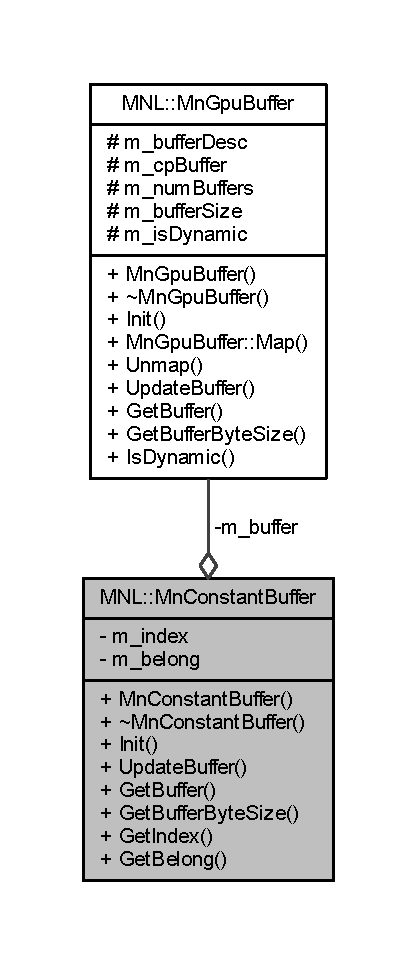
\includegraphics[width=200pt]{class_m_n_l_1_1_mn_constant_buffer__coll__graph}
\end{center}
\end{figure}
\subsection*{Public 멤버 함수}
\begin{DoxyCompactItemize}
\item 
\hyperlink{class_m_n_l_1_1_mn_constant_buffer_a1ee7c81dedfacf937bef2831f5f296d2}{Mn\+Constant\+Buffer} ()
\item 
\hyperlink{class_m_n_l_1_1_mn_constant_buffer_a03796084c5f1842880022fb1024162ae}{$\sim$\+Mn\+Constant\+Buffer} ()
\item 
H\+R\+E\+S\+U\+LT \hyperlink{class_m_n_l_1_1_mn_constant_buffer_a16b6059a895eb7da76323aaffe61e915}{Init} (const \hyperlink{namespace_m_n_l_a1eec210db8f309a4a9ac0d9658784c31}{C\+P\+D3\+D\+Device} \&cp\+Device, const std\+::shared\+\_\+ptr$<$ \hyperlink{class_m_n_l_1_1_mn_constant_buffer_type}{Mn\+Constant\+Buffer\+Type} $>$ \&constant\+Buffer\+Type, U\+I\+NT index, const \hyperlink{namespace_m_n_l_a3f526411258a17023ecac1a36e666d42}{M\+N\+\_\+\+C\+O\+N\+S\+T\+A\+N\+T\+\_\+\+B\+U\+F\+F\+E\+R\+\_\+\+B\+E\+L\+O\+NG} \&constant\+Buffer\+Belong)
\item 
void \hyperlink{class_m_n_l_1_1_mn_constant_buffer_a35ca3bffb4e5a497fe2303b1fa3abae4}{Update\+Buffer} (\hyperlink{namespace_m_n_l_aab3aabb6c9360e44ddc8b0bb563c2107}{C\+P\+D3\+D\+Device\+Context} cp\+Device\+Context, const D3\+D11\+\_\+\+S\+U\+B\+R\+E\+S\+O\+U\+R\+C\+E\+\_\+\+D\+A\+TA \&data)
\item 
const \hyperlink{namespace_m_n_l_aab9c90a8c27ac6410a9cc7cd89efeef1}{C\+P\+D3\+D\+Buffer} \hyperlink{class_m_n_l_1_1_mn_constant_buffer_a313d7555609f87dc0f104b2a19ce3c87}{Get\+Buffer} () const
\item 
U\+I\+NT \hyperlink{class_m_n_l_1_1_mn_constant_buffer_ac5cec5ad72abe2c7659d4ee29d6b6cf9}{Get\+Buffer\+Byte\+Size} () const
\item 
U\+I\+NT \hyperlink{class_m_n_l_1_1_mn_constant_buffer_a7b39b7ae15b314a6d12de1181d5ff180}{Get\+Index} () const
\item 
\hyperlink{namespace_m_n_l_a3f526411258a17023ecac1a36e666d42}{M\+N\+\_\+\+C\+O\+N\+S\+T\+A\+N\+T\+\_\+\+B\+U\+F\+F\+E\+R\+\_\+\+B\+E\+L\+O\+NG} \hyperlink{class_m_n_l_1_1_mn_constant_buffer_aadb464e8b09a7c1602681842b583b6f8}{Get\+Belong} () const
\end{DoxyCompactItemize}
\subsection*{Private 속성}
\begin{DoxyCompactItemize}
\item 
\hyperlink{class_m_n_l_1_1_mn_gpu_buffer}{Mn\+Gpu\+Buffer} \hyperlink{class_m_n_l_1_1_mn_constant_buffer_a1a9d69098ff55f524716d8415fe76e20}{m\+\_\+buffer}
\item 
U\+I\+NT \hyperlink{class_m_n_l_1_1_mn_constant_buffer_a2ae6082ec83ef177993de6235b0030a1}{m\+\_\+index}
\item 
\hyperlink{namespace_m_n_l_a3f526411258a17023ecac1a36e666d42}{M\+N\+\_\+\+C\+O\+N\+S\+T\+A\+N\+T\+\_\+\+B\+U\+F\+F\+E\+R\+\_\+\+B\+E\+L\+O\+NG} \hyperlink{class_m_n_l_1_1_mn_constant_buffer_aaab10bc1257803aba45c924acab04c35}{m\+\_\+belong}
\end{DoxyCompactItemize}


\subsection{상세한 설명}


Mn\+Constant\+Buffer.\+h 파일의 19 번째 라인에서 정의되었습니다.



\subsection{생성자 \& 소멸자 문서화}
\mbox{\Hypertarget{class_m_n_l_1_1_mn_constant_buffer_a1ee7c81dedfacf937bef2831f5f296d2}\label{class_m_n_l_1_1_mn_constant_buffer_a1ee7c81dedfacf937bef2831f5f296d2}} 
\index{M\+N\+L\+::\+Mn\+Constant\+Buffer@{M\+N\+L\+::\+Mn\+Constant\+Buffer}!Mn\+Constant\+Buffer@{Mn\+Constant\+Buffer}}
\index{Mn\+Constant\+Buffer@{Mn\+Constant\+Buffer}!M\+N\+L\+::\+Mn\+Constant\+Buffer@{M\+N\+L\+::\+Mn\+Constant\+Buffer}}
\subsubsection{\texorpdfstring{Mn\+Constant\+Buffer()}{MnConstantBuffer()}}
{\footnotesize\ttfamily Mn\+Constant\+Buffer\+::\+Mn\+Constant\+Buffer (\begin{DoxyParamCaption}{ }\end{DoxyParamCaption})}



Mn\+Constant\+Buffer.\+cpp 파일의 6 번째 라인에서 정의되었습니다.

\mbox{\Hypertarget{class_m_n_l_1_1_mn_constant_buffer_a03796084c5f1842880022fb1024162ae}\label{class_m_n_l_1_1_mn_constant_buffer_a03796084c5f1842880022fb1024162ae}} 
\index{M\+N\+L\+::\+Mn\+Constant\+Buffer@{M\+N\+L\+::\+Mn\+Constant\+Buffer}!````~Mn\+Constant\+Buffer@{$\sim$\+Mn\+Constant\+Buffer}}
\index{````~Mn\+Constant\+Buffer@{$\sim$\+Mn\+Constant\+Buffer}!M\+N\+L\+::\+Mn\+Constant\+Buffer@{M\+N\+L\+::\+Mn\+Constant\+Buffer}}
\subsubsection{\texorpdfstring{$\sim$\+Mn\+Constant\+Buffer()}{~MnConstantBuffer()}}
{\footnotesize\ttfamily Mn\+Constant\+Buffer\+::$\sim$\+Mn\+Constant\+Buffer (\begin{DoxyParamCaption}{ }\end{DoxyParamCaption})}



Mn\+Constant\+Buffer.\+cpp 파일의 11 번째 라인에서 정의되었습니다.



\subsection{멤버 함수 문서화}
\mbox{\Hypertarget{class_m_n_l_1_1_mn_constant_buffer_aadb464e8b09a7c1602681842b583b6f8}\label{class_m_n_l_1_1_mn_constant_buffer_aadb464e8b09a7c1602681842b583b6f8}} 
\index{M\+N\+L\+::\+Mn\+Constant\+Buffer@{M\+N\+L\+::\+Mn\+Constant\+Buffer}!Get\+Belong@{Get\+Belong}}
\index{Get\+Belong@{Get\+Belong}!M\+N\+L\+::\+Mn\+Constant\+Buffer@{M\+N\+L\+::\+Mn\+Constant\+Buffer}}
\subsubsection{\texorpdfstring{Get\+Belong()}{GetBelong()}}
{\footnotesize\ttfamily \hyperlink{namespace_m_n_l_a3f526411258a17023ecac1a36e666d42}{M\+N\+\_\+\+C\+O\+N\+S\+T\+A\+N\+T\+\_\+\+B\+U\+F\+F\+E\+R\+\_\+\+B\+E\+L\+O\+NG} Mn\+Constant\+Buffer\+::\+Get\+Belong (\begin{DoxyParamCaption}{ }\end{DoxyParamCaption}) const}



Mn\+Constant\+Buffer.\+cpp 파일의 58 번째 라인에서 정의되었습니다.

\mbox{\Hypertarget{class_m_n_l_1_1_mn_constant_buffer_a313d7555609f87dc0f104b2a19ce3c87}\label{class_m_n_l_1_1_mn_constant_buffer_a313d7555609f87dc0f104b2a19ce3c87}} 
\index{M\+N\+L\+::\+Mn\+Constant\+Buffer@{M\+N\+L\+::\+Mn\+Constant\+Buffer}!Get\+Buffer@{Get\+Buffer}}
\index{Get\+Buffer@{Get\+Buffer}!M\+N\+L\+::\+Mn\+Constant\+Buffer@{M\+N\+L\+::\+Mn\+Constant\+Buffer}}
\subsubsection{\texorpdfstring{Get\+Buffer()}{GetBuffer()}}
{\footnotesize\ttfamily const \hyperlink{namespace_m_n_l_aab9c90a8c27ac6410a9cc7cd89efeef1}{C\+P\+D3\+D\+Buffer} Mn\+Constant\+Buffer\+::\+Get\+Buffer (\begin{DoxyParamCaption}{ }\end{DoxyParamCaption}) const}



Mn\+Constant\+Buffer.\+cpp 파일의 44 번째 라인에서 정의되었습니다.

\mbox{\Hypertarget{class_m_n_l_1_1_mn_constant_buffer_ac5cec5ad72abe2c7659d4ee29d6b6cf9}\label{class_m_n_l_1_1_mn_constant_buffer_ac5cec5ad72abe2c7659d4ee29d6b6cf9}} 
\index{M\+N\+L\+::\+Mn\+Constant\+Buffer@{M\+N\+L\+::\+Mn\+Constant\+Buffer}!Get\+Buffer\+Byte\+Size@{Get\+Buffer\+Byte\+Size}}
\index{Get\+Buffer\+Byte\+Size@{Get\+Buffer\+Byte\+Size}!M\+N\+L\+::\+Mn\+Constant\+Buffer@{M\+N\+L\+::\+Mn\+Constant\+Buffer}}
\subsubsection{\texorpdfstring{Get\+Buffer\+Byte\+Size()}{GetBufferByteSize()}}
{\footnotesize\ttfamily U\+I\+NT Mn\+Constant\+Buffer\+::\+Get\+Buffer\+Byte\+Size (\begin{DoxyParamCaption}{ }\end{DoxyParamCaption}) const}



Mn\+Constant\+Buffer.\+cpp 파일의 48 번째 라인에서 정의되었습니다.

\mbox{\Hypertarget{class_m_n_l_1_1_mn_constant_buffer_a7b39b7ae15b314a6d12de1181d5ff180}\label{class_m_n_l_1_1_mn_constant_buffer_a7b39b7ae15b314a6d12de1181d5ff180}} 
\index{M\+N\+L\+::\+Mn\+Constant\+Buffer@{M\+N\+L\+::\+Mn\+Constant\+Buffer}!Get\+Index@{Get\+Index}}
\index{Get\+Index@{Get\+Index}!M\+N\+L\+::\+Mn\+Constant\+Buffer@{M\+N\+L\+::\+Mn\+Constant\+Buffer}}
\subsubsection{\texorpdfstring{Get\+Index()}{GetIndex()}}
{\footnotesize\ttfamily U\+I\+NT Mn\+Constant\+Buffer\+::\+Get\+Index (\begin{DoxyParamCaption}{ }\end{DoxyParamCaption}) const}



Mn\+Constant\+Buffer.\+cpp 파일의 53 번째 라인에서 정의되었습니다.

\mbox{\Hypertarget{class_m_n_l_1_1_mn_constant_buffer_a16b6059a895eb7da76323aaffe61e915}\label{class_m_n_l_1_1_mn_constant_buffer_a16b6059a895eb7da76323aaffe61e915}} 
\index{M\+N\+L\+::\+Mn\+Constant\+Buffer@{M\+N\+L\+::\+Mn\+Constant\+Buffer}!Init@{Init}}
\index{Init@{Init}!M\+N\+L\+::\+Mn\+Constant\+Buffer@{M\+N\+L\+::\+Mn\+Constant\+Buffer}}
\subsubsection{\texorpdfstring{Init()}{Init()}}
{\footnotesize\ttfamily H\+R\+E\+S\+U\+LT Mn\+Constant\+Buffer\+::\+Init (\begin{DoxyParamCaption}\item[{const \hyperlink{namespace_m_n_l_a1eec210db8f309a4a9ac0d9658784c31}{C\+P\+D3\+D\+Device} \&}]{cp\+Device,  }\item[{const std\+::shared\+\_\+ptr$<$ \hyperlink{class_m_n_l_1_1_mn_constant_buffer_type}{Mn\+Constant\+Buffer\+Type} $>$ \&}]{constant\+Buffer\+Type,  }\item[{U\+I\+NT}]{index,  }\item[{const \hyperlink{namespace_m_n_l_a3f526411258a17023ecac1a36e666d42}{M\+N\+\_\+\+C\+O\+N\+S\+T\+A\+N\+T\+\_\+\+B\+U\+F\+F\+E\+R\+\_\+\+B\+E\+L\+O\+NG} \&}]{constant\+Buffer\+Belong }\end{DoxyParamCaption})}



Mn\+Constant\+Buffer.\+cpp 파일의 16 번째 라인에서 정의되었습니다.

\mbox{\Hypertarget{class_m_n_l_1_1_mn_constant_buffer_a35ca3bffb4e5a497fe2303b1fa3abae4}\label{class_m_n_l_1_1_mn_constant_buffer_a35ca3bffb4e5a497fe2303b1fa3abae4}} 
\index{M\+N\+L\+::\+Mn\+Constant\+Buffer@{M\+N\+L\+::\+Mn\+Constant\+Buffer}!Update\+Buffer@{Update\+Buffer}}
\index{Update\+Buffer@{Update\+Buffer}!M\+N\+L\+::\+Mn\+Constant\+Buffer@{M\+N\+L\+::\+Mn\+Constant\+Buffer}}
\subsubsection{\texorpdfstring{Update\+Buffer()}{UpdateBuffer()}}
{\footnotesize\ttfamily void Mn\+Constant\+Buffer\+::\+Update\+Buffer (\begin{DoxyParamCaption}\item[{\hyperlink{namespace_m_n_l_aab3aabb6c9360e44ddc8b0bb563c2107}{C\+P\+D3\+D\+Device\+Context}}]{cp\+Device\+Context,  }\item[{const D3\+D11\+\_\+\+S\+U\+B\+R\+E\+S\+O\+U\+R\+C\+E\+\_\+\+D\+A\+TA \&}]{data }\end{DoxyParamCaption})}

Create D3\+D11\+\_\+\+S\+U\+B\+R\+E\+S\+O\+U\+R\+C\+E\+\_\+\+D\+A\+TA, set p\+Sys\+Mem link to the user created own structrue(must be same byte size as constant buffer type), then transfer as parameter. 

Mn\+Constant\+Buffer.\+cpp 파일의 39 번째 라인에서 정의되었습니다.



\subsection{멤버 데이터 문서화}
\mbox{\Hypertarget{class_m_n_l_1_1_mn_constant_buffer_aaab10bc1257803aba45c924acab04c35}\label{class_m_n_l_1_1_mn_constant_buffer_aaab10bc1257803aba45c924acab04c35}} 
\index{M\+N\+L\+::\+Mn\+Constant\+Buffer@{M\+N\+L\+::\+Mn\+Constant\+Buffer}!m\+\_\+belong@{m\+\_\+belong}}
\index{m\+\_\+belong@{m\+\_\+belong}!M\+N\+L\+::\+Mn\+Constant\+Buffer@{M\+N\+L\+::\+Mn\+Constant\+Buffer}}
\subsubsection{\texorpdfstring{m\+\_\+belong}{m\_belong}}
{\footnotesize\ttfamily \hyperlink{namespace_m_n_l_a3f526411258a17023ecac1a36e666d42}{M\+N\+\_\+\+C\+O\+N\+S\+T\+A\+N\+T\+\_\+\+B\+U\+F\+F\+E\+R\+\_\+\+B\+E\+L\+O\+NG} M\+N\+L\+::\+Mn\+Constant\+Buffer\+::m\+\_\+belong\hspace{0.3cm}{\ttfamily [private]}}



Mn\+Constant\+Buffer.\+h 파일의 42 번째 라인에서 정의되었습니다.

\mbox{\Hypertarget{class_m_n_l_1_1_mn_constant_buffer_a1a9d69098ff55f524716d8415fe76e20}\label{class_m_n_l_1_1_mn_constant_buffer_a1a9d69098ff55f524716d8415fe76e20}} 
\index{M\+N\+L\+::\+Mn\+Constant\+Buffer@{M\+N\+L\+::\+Mn\+Constant\+Buffer}!m\+\_\+buffer@{m\+\_\+buffer}}
\index{m\+\_\+buffer@{m\+\_\+buffer}!M\+N\+L\+::\+Mn\+Constant\+Buffer@{M\+N\+L\+::\+Mn\+Constant\+Buffer}}
\subsubsection{\texorpdfstring{m\+\_\+buffer}{m\_buffer}}
{\footnotesize\ttfamily \hyperlink{class_m_n_l_1_1_mn_gpu_buffer}{Mn\+Gpu\+Buffer} M\+N\+L\+::\+Mn\+Constant\+Buffer\+::m\+\_\+buffer\hspace{0.3cm}{\ttfamily [private]}}



Mn\+Constant\+Buffer.\+h 파일의 40 번째 라인에서 정의되었습니다.

\mbox{\Hypertarget{class_m_n_l_1_1_mn_constant_buffer_a2ae6082ec83ef177993de6235b0030a1}\label{class_m_n_l_1_1_mn_constant_buffer_a2ae6082ec83ef177993de6235b0030a1}} 
\index{M\+N\+L\+::\+Mn\+Constant\+Buffer@{M\+N\+L\+::\+Mn\+Constant\+Buffer}!m\+\_\+index@{m\+\_\+index}}
\index{m\+\_\+index@{m\+\_\+index}!M\+N\+L\+::\+Mn\+Constant\+Buffer@{M\+N\+L\+::\+Mn\+Constant\+Buffer}}
\subsubsection{\texorpdfstring{m\+\_\+index}{m\_index}}
{\footnotesize\ttfamily U\+I\+NT M\+N\+L\+::\+Mn\+Constant\+Buffer\+::m\+\_\+index\hspace{0.3cm}{\ttfamily [private]}}



Mn\+Constant\+Buffer.\+h 파일의 41 번째 라인에서 정의되었습니다.



이 클래스에 대한 문서화 페이지는 다음의 파일들로부터 생성되었습니다.\+:\begin{DoxyCompactItemize}
\item 
Core/\hyperlink{_mn_constant_buffer_8h}{Mn\+Constant\+Buffer.\+h}\item 
Core/\hyperlink{_mn_constant_buffer_8cpp}{Mn\+Constant\+Buffer.\+cpp}\end{DoxyCompactItemize}

\hypertarget{class_m_n_l_1_1_mn_constant_buffer_type}{}\section{M\+NL\+:\+:Mn\+Constant\+Buffer\+Type 클래스 참조}
\label{class_m_n_l_1_1_mn_constant_buffer_type}\index{M\+N\+L\+::\+Mn\+Constant\+Buffer\+Type@{M\+N\+L\+::\+Mn\+Constant\+Buffer\+Type}}


{\ttfamily \#include $<$Mn\+Constant\+Buffer\+Type.\+h$>$}



M\+NL\+:\+:Mn\+Constant\+Buffer\+Type에 대한 협력 다이어그램\+:\nopagebreak
\begin{figure}[H]
\begin{center}
\leavevmode
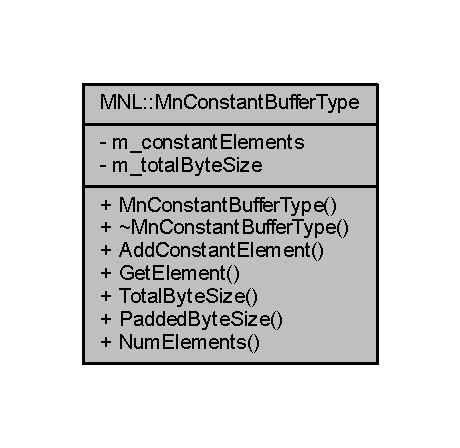
\includegraphics[width=221pt]{class_m_n_l_1_1_mn_constant_buffer_type__coll__graph}
\end{center}
\end{figure}
\subsection*{Public 멤버 함수}
\begin{DoxyCompactItemize}
\item 
\hyperlink{class_m_n_l_1_1_mn_constant_buffer_type_adb400b9153ea587f4f1ed5173c9fe0e5}{Mn\+Constant\+Buffer\+Type} ()
\item 
\hyperlink{class_m_n_l_1_1_mn_constant_buffer_type_a379082879b3a4e9220ea3ded514b8982}{$\sim$\+Mn\+Constant\+Buffer\+Type} ()
\item 
void \hyperlink{class_m_n_l_1_1_mn_constant_buffer_type_ae9221d7fff984c158938611cf05666dc}{Add\+Constant\+Element} (const \hyperlink{class_m_n_l_1_1_mn_constant_element}{Mn\+Constant\+Element} \&input\+Element)
\item 
const \hyperlink{class_m_n_l_1_1_mn_constant_element}{Mn\+Constant\+Element} \& \hyperlink{class_m_n_l_1_1_mn_constant_buffer_type_a4e5740ac5ebdcf8dc0473721c0a6391f}{Get\+Element} (U\+I\+NT index) const
\item 
U\+I\+NT \hyperlink{class_m_n_l_1_1_mn_constant_buffer_type_aae1e8677534067f7019df4326ddfaf4d}{Total\+Byte\+Size} () const
\item 
U\+I\+NT \hyperlink{class_m_n_l_1_1_mn_constant_buffer_type_a12c8039ed9335db7db09f9628347080c}{Padded\+Byte\+Size} () const
\item 
U\+I\+NT \hyperlink{class_m_n_l_1_1_mn_constant_buffer_type_a1f7946e71fb2708c4e43066cb99cba4f}{Num\+Elements} () const
\end{DoxyCompactItemize}
\subsection*{Private 속성}
\begin{DoxyCompactItemize}
\item 
std\+::vector$<$ \hyperlink{class_m_n_l_1_1_mn_constant_element}{Mn\+Constant\+Element} $>$ \hyperlink{class_m_n_l_1_1_mn_constant_buffer_type_abbcebdac92c25f66a090acb6b902573d}{m\+\_\+constant\+Elements}
\item 
U\+I\+NT \hyperlink{class_m_n_l_1_1_mn_constant_buffer_type_a27af6863155a8cc6edb48df620a86b56}{m\+\_\+total\+Byte\+Size}
\end{DoxyCompactItemize}


\subsection{상세한 설명}


Mn\+Constant\+Buffer\+Type.\+h 파일의 12 번째 라인에서 정의되었습니다.



\subsection{생성자 \& 소멸자 문서화}
\mbox{\Hypertarget{class_m_n_l_1_1_mn_constant_buffer_type_adb400b9153ea587f4f1ed5173c9fe0e5}\label{class_m_n_l_1_1_mn_constant_buffer_type_adb400b9153ea587f4f1ed5173c9fe0e5}} 
\index{M\+N\+L\+::\+Mn\+Constant\+Buffer\+Type@{M\+N\+L\+::\+Mn\+Constant\+Buffer\+Type}!Mn\+Constant\+Buffer\+Type@{Mn\+Constant\+Buffer\+Type}}
\index{Mn\+Constant\+Buffer\+Type@{Mn\+Constant\+Buffer\+Type}!M\+N\+L\+::\+Mn\+Constant\+Buffer\+Type@{M\+N\+L\+::\+Mn\+Constant\+Buffer\+Type}}
\subsubsection{\texorpdfstring{Mn\+Constant\+Buffer\+Type()}{MnConstantBufferType()}}
{\footnotesize\ttfamily Mn\+Constant\+Buffer\+Type\+::\+Mn\+Constant\+Buffer\+Type (\begin{DoxyParamCaption}{ }\end{DoxyParamCaption})}



Mn\+Constant\+Buffer\+Type.\+cpp 파일의 5 번째 라인에서 정의되었습니다.

\mbox{\Hypertarget{class_m_n_l_1_1_mn_constant_buffer_type_a379082879b3a4e9220ea3ded514b8982}\label{class_m_n_l_1_1_mn_constant_buffer_type_a379082879b3a4e9220ea3ded514b8982}} 
\index{M\+N\+L\+::\+Mn\+Constant\+Buffer\+Type@{M\+N\+L\+::\+Mn\+Constant\+Buffer\+Type}!````~Mn\+Constant\+Buffer\+Type@{$\sim$\+Mn\+Constant\+Buffer\+Type}}
\index{````~Mn\+Constant\+Buffer\+Type@{$\sim$\+Mn\+Constant\+Buffer\+Type}!M\+N\+L\+::\+Mn\+Constant\+Buffer\+Type@{M\+N\+L\+::\+Mn\+Constant\+Buffer\+Type}}
\subsubsection{\texorpdfstring{$\sim$\+Mn\+Constant\+Buffer\+Type()}{~MnConstantBufferType()}}
{\footnotesize\ttfamily Mn\+Constant\+Buffer\+Type\+::$\sim$\+Mn\+Constant\+Buffer\+Type (\begin{DoxyParamCaption}{ }\end{DoxyParamCaption})}



Mn\+Constant\+Buffer\+Type.\+cpp 파일의 10 번째 라인에서 정의되었습니다.



\subsection{멤버 함수 문서화}
\mbox{\Hypertarget{class_m_n_l_1_1_mn_constant_buffer_type_ae9221d7fff984c158938611cf05666dc}\label{class_m_n_l_1_1_mn_constant_buffer_type_ae9221d7fff984c158938611cf05666dc}} 
\index{M\+N\+L\+::\+Mn\+Constant\+Buffer\+Type@{M\+N\+L\+::\+Mn\+Constant\+Buffer\+Type}!Add\+Constant\+Element@{Add\+Constant\+Element}}
\index{Add\+Constant\+Element@{Add\+Constant\+Element}!M\+N\+L\+::\+Mn\+Constant\+Buffer\+Type@{M\+N\+L\+::\+Mn\+Constant\+Buffer\+Type}}
\subsubsection{\texorpdfstring{Add\+Constant\+Element()}{AddConstantElement()}}
{\footnotesize\ttfamily void Mn\+Constant\+Buffer\+Type\+::\+Add\+Constant\+Element (\begin{DoxyParamCaption}\item[{const \hyperlink{class_m_n_l_1_1_mn_constant_element}{Mn\+Constant\+Element} \&}]{input\+Element }\end{DoxyParamCaption})}

Add a input element to description. input layout will be placed by adding order 

Mn\+Constant\+Buffer\+Type.\+cpp 파일의 14 번째 라인에서 정의되었습니다.

\mbox{\Hypertarget{class_m_n_l_1_1_mn_constant_buffer_type_a4e5740ac5ebdcf8dc0473721c0a6391f}\label{class_m_n_l_1_1_mn_constant_buffer_type_a4e5740ac5ebdcf8dc0473721c0a6391f}} 
\index{M\+N\+L\+::\+Mn\+Constant\+Buffer\+Type@{M\+N\+L\+::\+Mn\+Constant\+Buffer\+Type}!Get\+Element@{Get\+Element}}
\index{Get\+Element@{Get\+Element}!M\+N\+L\+::\+Mn\+Constant\+Buffer\+Type@{M\+N\+L\+::\+Mn\+Constant\+Buffer\+Type}}
\subsubsection{\texorpdfstring{Get\+Element()}{GetElement()}}
{\footnotesize\ttfamily const \hyperlink{class_m_n_l_1_1_mn_constant_element}{Mn\+Constant\+Element} \& Mn\+Constant\+Buffer\+Type\+::\+Get\+Element (\begin{DoxyParamCaption}\item[{U\+I\+NT}]{index }\end{DoxyParamCaption}) const}

Get a input element 
\begin{DoxyParams}{매개변수}
{\em index} & of the input elemenet \\
\hline
\end{DoxyParams}


Mn\+Constant\+Buffer\+Type.\+cpp 파일의 19 번째 라인에서 정의되었습니다.

\mbox{\Hypertarget{class_m_n_l_1_1_mn_constant_buffer_type_a1f7946e71fb2708c4e43066cb99cba4f}\label{class_m_n_l_1_1_mn_constant_buffer_type_a1f7946e71fb2708c4e43066cb99cba4f}} 
\index{M\+N\+L\+::\+Mn\+Constant\+Buffer\+Type@{M\+N\+L\+::\+Mn\+Constant\+Buffer\+Type}!Num\+Elements@{Num\+Elements}}
\index{Num\+Elements@{Num\+Elements}!M\+N\+L\+::\+Mn\+Constant\+Buffer\+Type@{M\+N\+L\+::\+Mn\+Constant\+Buffer\+Type}}
\subsubsection{\texorpdfstring{Num\+Elements()}{NumElements()}}
{\footnotesize\ttfamily U\+I\+NT Mn\+Constant\+Buffer\+Type\+::\+Num\+Elements (\begin{DoxyParamCaption}{ }\end{DoxyParamCaption}) const}

\begin{DoxyReturn}{반환값}
count of input elements 
\end{DoxyReturn}


Mn\+Constant\+Buffer\+Type.\+cpp 파일의 32 번째 라인에서 정의되었습니다.

\mbox{\Hypertarget{class_m_n_l_1_1_mn_constant_buffer_type_a12c8039ed9335db7db09f9628347080c}\label{class_m_n_l_1_1_mn_constant_buffer_type_a12c8039ed9335db7db09f9628347080c}} 
\index{M\+N\+L\+::\+Mn\+Constant\+Buffer\+Type@{M\+N\+L\+::\+Mn\+Constant\+Buffer\+Type}!Padded\+Byte\+Size@{Padded\+Byte\+Size}}
\index{Padded\+Byte\+Size@{Padded\+Byte\+Size}!M\+N\+L\+::\+Mn\+Constant\+Buffer\+Type@{M\+N\+L\+::\+Mn\+Constant\+Buffer\+Type}}
\subsubsection{\texorpdfstring{Padded\+Byte\+Size()}{PaddedByteSize()}}
{\footnotesize\ttfamily U\+I\+NT Mn\+Constant\+Buffer\+Type\+::\+Padded\+Byte\+Size (\begin{DoxyParamCaption}{ }\end{DoxyParamCaption}) const}



Mn\+Constant\+Buffer\+Type.\+cpp 파일의 28 번째 라인에서 정의되었습니다.

\mbox{\Hypertarget{class_m_n_l_1_1_mn_constant_buffer_type_aae1e8677534067f7019df4326ddfaf4d}\label{class_m_n_l_1_1_mn_constant_buffer_type_aae1e8677534067f7019df4326ddfaf4d}} 
\index{M\+N\+L\+::\+Mn\+Constant\+Buffer\+Type@{M\+N\+L\+::\+Mn\+Constant\+Buffer\+Type}!Total\+Byte\+Size@{Total\+Byte\+Size}}
\index{Total\+Byte\+Size@{Total\+Byte\+Size}!M\+N\+L\+::\+Mn\+Constant\+Buffer\+Type@{M\+N\+L\+::\+Mn\+Constant\+Buffer\+Type}}
\subsubsection{\texorpdfstring{Total\+Byte\+Size()}{TotalByteSize()}}
{\footnotesize\ttfamily U\+I\+NT Mn\+Constant\+Buffer\+Type\+::\+Total\+Byte\+Size (\begin{DoxyParamCaption}{ }\end{DoxyParamCaption}) const}

\begin{DoxyReturn}{반환값}
total byte size of whole constant elements 
\end{DoxyReturn}


Mn\+Constant\+Buffer\+Type.\+cpp 파일의 24 번째 라인에서 정의되었습니다.



\subsection{멤버 데이터 문서화}
\mbox{\Hypertarget{class_m_n_l_1_1_mn_constant_buffer_type_abbcebdac92c25f66a090acb6b902573d}\label{class_m_n_l_1_1_mn_constant_buffer_type_abbcebdac92c25f66a090acb6b902573d}} 
\index{M\+N\+L\+::\+Mn\+Constant\+Buffer\+Type@{M\+N\+L\+::\+Mn\+Constant\+Buffer\+Type}!m\+\_\+constant\+Elements@{m\+\_\+constant\+Elements}}
\index{m\+\_\+constant\+Elements@{m\+\_\+constant\+Elements}!M\+N\+L\+::\+Mn\+Constant\+Buffer\+Type@{M\+N\+L\+::\+Mn\+Constant\+Buffer\+Type}}
\subsubsection{\texorpdfstring{m\+\_\+constant\+Elements}{m\_constantElements}}
{\footnotesize\ttfamily std\+::vector$<$\hyperlink{class_m_n_l_1_1_mn_constant_element}{Mn\+Constant\+Element}$>$ M\+N\+L\+::\+Mn\+Constant\+Buffer\+Type\+::m\+\_\+constant\+Elements\hspace{0.3cm}{\ttfamily [private]}}



Mn\+Constant\+Buffer\+Type.\+h 파일의 42 번째 라인에서 정의되었습니다.

\mbox{\Hypertarget{class_m_n_l_1_1_mn_constant_buffer_type_a27af6863155a8cc6edb48df620a86b56}\label{class_m_n_l_1_1_mn_constant_buffer_type_a27af6863155a8cc6edb48df620a86b56}} 
\index{M\+N\+L\+::\+Mn\+Constant\+Buffer\+Type@{M\+N\+L\+::\+Mn\+Constant\+Buffer\+Type}!m\+\_\+total\+Byte\+Size@{m\+\_\+total\+Byte\+Size}}
\index{m\+\_\+total\+Byte\+Size@{m\+\_\+total\+Byte\+Size}!M\+N\+L\+::\+Mn\+Constant\+Buffer\+Type@{M\+N\+L\+::\+Mn\+Constant\+Buffer\+Type}}
\subsubsection{\texorpdfstring{m\+\_\+total\+Byte\+Size}{m\_totalByteSize}}
{\footnotesize\ttfamily U\+I\+NT M\+N\+L\+::\+Mn\+Constant\+Buffer\+Type\+::m\+\_\+total\+Byte\+Size\hspace{0.3cm}{\ttfamily [private]}}



Mn\+Constant\+Buffer\+Type.\+h 파일의 43 번째 라인에서 정의되었습니다.



이 클래스에 대한 문서화 페이지는 다음의 파일들로부터 생성되었습니다.\+:\begin{DoxyCompactItemize}
\item 
Core/\hyperlink{_mn_constant_buffer_type_8h}{Mn\+Constant\+Buffer\+Type.\+h}\item 
Core/\hyperlink{_mn_constant_buffer_type_8cpp}{Mn\+Constant\+Buffer\+Type.\+cpp}\end{DoxyCompactItemize}

\hypertarget{class_m_n_l_1_1_mn_constant_element}{}\section{M\+NL\+:\+:Mn\+Constant\+Element 클래스 참조}
\label{class_m_n_l_1_1_mn_constant_element}\index{M\+N\+L\+::\+Mn\+Constant\+Element@{M\+N\+L\+::\+Mn\+Constant\+Element}}


{\ttfamily \#include $<$Mn\+Constant\+Element.\+h$>$}



M\+NL\+:\+:Mn\+Constant\+Element에 대한 협력 다이어그램\+:\nopagebreak
\begin{figure}[H]
\begin{center}
\leavevmode
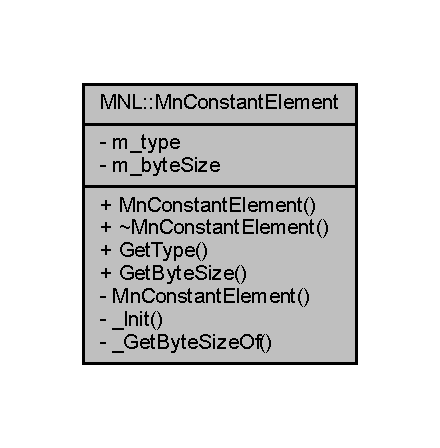
\includegraphics[width=211pt]{class_m_n_l_1_1_mn_constant_element__coll__graph}
\end{center}
\end{figure}
\subsection*{Public 멤버 함수}
\begin{DoxyCompactItemize}
\item 
\hyperlink{class_m_n_l_1_1_mn_constant_element_acf2d83e71ba0f23f91eb704bab1a3c44}{Mn\+Constant\+Element} (const \hyperlink{namespace_m_n_l_a7d0c6fcd5ada7e43f4059b8a9b4afb49}{Mn\+Constant\+Element\+Type} \&input\+Element\+Type)
\item 
\hyperlink{class_m_n_l_1_1_mn_constant_element_a3bde989f21552b8cc4e027934a7cd766}{$\sim$\+Mn\+Constant\+Element} ()
\item 
\hyperlink{namespace_m_n_l_a7d0c6fcd5ada7e43f4059b8a9b4afb49}{Mn\+Constant\+Element\+Type} \hyperlink{class_m_n_l_1_1_mn_constant_element_adf574d682e379192b4f84e108f22b31f}{Get\+Type} () const
\item 
U\+I\+NT \hyperlink{class_m_n_l_1_1_mn_constant_element_a9db6b1f129ac9630959bf8b9c3cff804}{Get\+Byte\+Size} () const
\end{DoxyCompactItemize}
\subsection*{Private 멤버 함수}
\begin{DoxyCompactItemize}
\item 
\hyperlink{class_m_n_l_1_1_mn_constant_element_aae694955b2ffd802eeb59034e889c62b}{Mn\+Constant\+Element} ()
\item 
H\+R\+E\+S\+U\+LT \hyperlink{class_m_n_l_1_1_mn_constant_element_a226616b9e6e135a920943803bd8d651d}{\+\_\+\+Init} (const \hyperlink{namespace_m_n_l_a7d0c6fcd5ada7e43f4059b8a9b4afb49}{Mn\+Constant\+Element\+Type} \&constant\+Element\+Type)
\item 
U\+I\+NT \hyperlink{class_m_n_l_1_1_mn_constant_element_a34b4574387f535a74ab325a43649ceef}{\+\_\+\+Get\+Byte\+Size\+Of} (const \hyperlink{namespace_m_n_l_a7d0c6fcd5ada7e43f4059b8a9b4afb49}{Mn\+Constant\+Element\+Type} \&constant\+Element\+Type)
\end{DoxyCompactItemize}
\subsection*{Private 속성}
\begin{DoxyCompactItemize}
\item 
\hyperlink{namespace_m_n_l_a7d0c6fcd5ada7e43f4059b8a9b4afb49}{Mn\+Constant\+Element\+Type} \hyperlink{class_m_n_l_1_1_mn_constant_element_a6015e8f0784914bcb9e3beec92de11aa}{m\+\_\+type}
\item 
U\+I\+NT \hyperlink{class_m_n_l_1_1_mn_constant_element_a0b5df25aee74d374cd8f108137f7db6e}{m\+\_\+byte\+Size}
\end{DoxyCompactItemize}


\subsection{상세한 설명}


Mn\+Constant\+Element.\+h 파일의 20 번째 라인에서 정의되었습니다.



\subsection{생성자 \& 소멸자 문서화}
\mbox{\Hypertarget{class_m_n_l_1_1_mn_constant_element_acf2d83e71ba0f23f91eb704bab1a3c44}\label{class_m_n_l_1_1_mn_constant_element_acf2d83e71ba0f23f91eb704bab1a3c44}} 
\index{M\+N\+L\+::\+Mn\+Constant\+Element@{M\+N\+L\+::\+Mn\+Constant\+Element}!Mn\+Constant\+Element@{Mn\+Constant\+Element}}
\index{Mn\+Constant\+Element@{Mn\+Constant\+Element}!M\+N\+L\+::\+Mn\+Constant\+Element@{M\+N\+L\+::\+Mn\+Constant\+Element}}
\subsubsection{\texorpdfstring{Mn\+Constant\+Element()}{MnConstantElement()}\hspace{0.1cm}{\footnotesize\ttfamily [1/2]}}
{\footnotesize\ttfamily Mn\+Constant\+Element\+::\+Mn\+Constant\+Element (\begin{DoxyParamCaption}\item[{const \hyperlink{namespace_m_n_l_a7d0c6fcd5ada7e43f4059b8a9b4afb49}{Mn\+Constant\+Element\+Type} \&}]{input\+Element\+Type }\end{DoxyParamCaption})}



Mn\+Constant\+Element.\+cpp 파일의 14 번째 라인에서 정의되었습니다.

\mbox{\Hypertarget{class_m_n_l_1_1_mn_constant_element_a3bde989f21552b8cc4e027934a7cd766}\label{class_m_n_l_1_1_mn_constant_element_a3bde989f21552b8cc4e027934a7cd766}} 
\index{M\+N\+L\+::\+Mn\+Constant\+Element@{M\+N\+L\+::\+Mn\+Constant\+Element}!````~Mn\+Constant\+Element@{$\sim$\+Mn\+Constant\+Element}}
\index{````~Mn\+Constant\+Element@{$\sim$\+Mn\+Constant\+Element}!M\+N\+L\+::\+Mn\+Constant\+Element@{M\+N\+L\+::\+Mn\+Constant\+Element}}
\subsubsection{\texorpdfstring{$\sim$\+Mn\+Constant\+Element()}{~MnConstantElement()}}
{\footnotesize\ttfamily Mn\+Constant\+Element\+::$\sim$\+Mn\+Constant\+Element (\begin{DoxyParamCaption}{ }\end{DoxyParamCaption})}



Mn\+Constant\+Element.\+cpp 파일의 11 번째 라인에서 정의되었습니다.

\mbox{\Hypertarget{class_m_n_l_1_1_mn_constant_element_aae694955b2ffd802eeb59034e889c62b}\label{class_m_n_l_1_1_mn_constant_element_aae694955b2ffd802eeb59034e889c62b}} 
\index{M\+N\+L\+::\+Mn\+Constant\+Element@{M\+N\+L\+::\+Mn\+Constant\+Element}!Mn\+Constant\+Element@{Mn\+Constant\+Element}}
\index{Mn\+Constant\+Element@{Mn\+Constant\+Element}!M\+N\+L\+::\+Mn\+Constant\+Element@{M\+N\+L\+::\+Mn\+Constant\+Element}}
\subsubsection{\texorpdfstring{Mn\+Constant\+Element()}{MnConstantElement()}\hspace{0.1cm}{\footnotesize\ttfamily [2/2]}}
{\footnotesize\ttfamily Mn\+Constant\+Element\+::\+Mn\+Constant\+Element (\begin{DoxyParamCaption}{ }\end{DoxyParamCaption})\hspace{0.3cm}{\ttfamily [private]}}



Mn\+Constant\+Element.\+cpp 파일의 6 번째 라인에서 정의되었습니다.



\subsection{멤버 함수 문서화}
\mbox{\Hypertarget{class_m_n_l_1_1_mn_constant_element_a34b4574387f535a74ab325a43649ceef}\label{class_m_n_l_1_1_mn_constant_element_a34b4574387f535a74ab325a43649ceef}} 
\index{M\+N\+L\+::\+Mn\+Constant\+Element@{M\+N\+L\+::\+Mn\+Constant\+Element}!\+\_\+\+Get\+Byte\+Size\+Of@{\+\_\+\+Get\+Byte\+Size\+Of}}
\index{\+\_\+\+Get\+Byte\+Size\+Of@{\+\_\+\+Get\+Byte\+Size\+Of}!M\+N\+L\+::\+Mn\+Constant\+Element@{M\+N\+L\+::\+Mn\+Constant\+Element}}
\subsubsection{\texorpdfstring{\+\_\+\+Get\+Byte\+Size\+Of()}{\_GetByteSizeOf()}}
{\footnotesize\ttfamily U\+I\+NT Mn\+Constant\+Element\+::\+\_\+\+Get\+Byte\+Size\+Of (\begin{DoxyParamCaption}\item[{const \hyperlink{namespace_m_n_l_a7d0c6fcd5ada7e43f4059b8a9b4afb49}{Mn\+Constant\+Element\+Type} \&}]{constant\+Element\+Type }\end{DoxyParamCaption})\hspace{0.3cm}{\ttfamily [private]}}



Mn\+Constant\+Element.\+cpp 파일의 44 번째 라인에서 정의되었습니다.

\mbox{\Hypertarget{class_m_n_l_1_1_mn_constant_element_a226616b9e6e135a920943803bd8d651d}\label{class_m_n_l_1_1_mn_constant_element_a226616b9e6e135a920943803bd8d651d}} 
\index{M\+N\+L\+::\+Mn\+Constant\+Element@{M\+N\+L\+::\+Mn\+Constant\+Element}!\+\_\+\+Init@{\+\_\+\+Init}}
\index{\+\_\+\+Init@{\+\_\+\+Init}!M\+N\+L\+::\+Mn\+Constant\+Element@{M\+N\+L\+::\+Mn\+Constant\+Element}}
\subsubsection{\texorpdfstring{\+\_\+\+Init()}{\_Init()}}
{\footnotesize\ttfamily H\+R\+E\+S\+U\+LT Mn\+Constant\+Element\+::\+\_\+\+Init (\begin{DoxyParamCaption}\item[{const \hyperlink{namespace_m_n_l_a7d0c6fcd5ada7e43f4059b8a9b4afb49}{Mn\+Constant\+Element\+Type} \&}]{constant\+Element\+Type }\end{DoxyParamCaption})\hspace{0.3cm}{\ttfamily [private]}}



Mn\+Constant\+Element.\+cpp 파일의 31 번째 라인에서 정의되었습니다.

\mbox{\Hypertarget{class_m_n_l_1_1_mn_constant_element_a9db6b1f129ac9630959bf8b9c3cff804}\label{class_m_n_l_1_1_mn_constant_element_a9db6b1f129ac9630959bf8b9c3cff804}} 
\index{M\+N\+L\+::\+Mn\+Constant\+Element@{M\+N\+L\+::\+Mn\+Constant\+Element}!Get\+Byte\+Size@{Get\+Byte\+Size}}
\index{Get\+Byte\+Size@{Get\+Byte\+Size}!M\+N\+L\+::\+Mn\+Constant\+Element@{M\+N\+L\+::\+Mn\+Constant\+Element}}
\subsubsection{\texorpdfstring{Get\+Byte\+Size()}{GetByteSize()}}
{\footnotesize\ttfamily U\+I\+NT Mn\+Constant\+Element\+::\+Get\+Byte\+Size (\begin{DoxyParamCaption}{ }\end{DoxyParamCaption}) const}



Mn\+Constant\+Element.\+cpp 파일의 26 번째 라인에서 정의되었습니다.

\mbox{\Hypertarget{class_m_n_l_1_1_mn_constant_element_adf574d682e379192b4f84e108f22b31f}\label{class_m_n_l_1_1_mn_constant_element_adf574d682e379192b4f84e108f22b31f}} 
\index{M\+N\+L\+::\+Mn\+Constant\+Element@{M\+N\+L\+::\+Mn\+Constant\+Element}!Get\+Type@{Get\+Type}}
\index{Get\+Type@{Get\+Type}!M\+N\+L\+::\+Mn\+Constant\+Element@{M\+N\+L\+::\+Mn\+Constant\+Element}}
\subsubsection{\texorpdfstring{Get\+Type()}{GetType()}}
{\footnotesize\ttfamily \hyperlink{namespace_m_n_l_a7d0c6fcd5ada7e43f4059b8a9b4afb49}{Mn\+Constant\+Element\+Type} Mn\+Constant\+Element\+::\+Get\+Type (\begin{DoxyParamCaption}{ }\end{DoxyParamCaption}) const}



Mn\+Constant\+Element.\+cpp 파일의 22 번째 라인에서 정의되었습니다.



\subsection{멤버 데이터 문서화}
\mbox{\Hypertarget{class_m_n_l_1_1_mn_constant_element_a0b5df25aee74d374cd8f108137f7db6e}\label{class_m_n_l_1_1_mn_constant_element_a0b5df25aee74d374cd8f108137f7db6e}} 
\index{M\+N\+L\+::\+Mn\+Constant\+Element@{M\+N\+L\+::\+Mn\+Constant\+Element}!m\+\_\+byte\+Size@{m\+\_\+byte\+Size}}
\index{m\+\_\+byte\+Size@{m\+\_\+byte\+Size}!M\+N\+L\+::\+Mn\+Constant\+Element@{M\+N\+L\+::\+Mn\+Constant\+Element}}
\subsubsection{\texorpdfstring{m\+\_\+byte\+Size}{m\_byteSize}}
{\footnotesize\ttfamily U\+I\+NT M\+N\+L\+::\+Mn\+Constant\+Element\+::m\+\_\+byte\+Size\hspace{0.3cm}{\ttfamily [private]}}



Mn\+Constant\+Element.\+h 파일의 39 번째 라인에서 정의되었습니다.

\mbox{\Hypertarget{class_m_n_l_1_1_mn_constant_element_a6015e8f0784914bcb9e3beec92de11aa}\label{class_m_n_l_1_1_mn_constant_element_a6015e8f0784914bcb9e3beec92de11aa}} 
\index{M\+N\+L\+::\+Mn\+Constant\+Element@{M\+N\+L\+::\+Mn\+Constant\+Element}!m\+\_\+type@{m\+\_\+type}}
\index{m\+\_\+type@{m\+\_\+type}!M\+N\+L\+::\+Mn\+Constant\+Element@{M\+N\+L\+::\+Mn\+Constant\+Element}}
\subsubsection{\texorpdfstring{m\+\_\+type}{m\_type}}
{\footnotesize\ttfamily \hyperlink{namespace_m_n_l_a7d0c6fcd5ada7e43f4059b8a9b4afb49}{Mn\+Constant\+Element\+Type} M\+N\+L\+::\+Mn\+Constant\+Element\+::m\+\_\+type\hspace{0.3cm}{\ttfamily [private]}}



Mn\+Constant\+Element.\+h 파일의 38 번째 라인에서 정의되었습니다.



이 클래스에 대한 문서화 페이지는 다음의 파일들로부터 생성되었습니다.\+:\begin{DoxyCompactItemize}
\item 
Core/\hyperlink{_mn_constant_element_8h}{Mn\+Constant\+Element.\+h}\item 
Core/\hyperlink{_mn_constant_element_8cpp}{Mn\+Constant\+Element.\+cpp}\end{DoxyCompactItemize}

\hypertarget{class_m_n_l_1_1_mn_custom_vertex_type}{}\section{M\+NL\+:\+:Mn\+Custom\+Vertex\+Type 클래스 참조}
\label{class_m_n_l_1_1_mn_custom_vertex_type}\index{M\+N\+L\+::\+Mn\+Custom\+Vertex\+Type@{M\+N\+L\+::\+Mn\+Custom\+Vertex\+Type}}


{\ttfamily \#include $<$Mn\+Custom\+Vertex\+Type.\+h$>$}



M\+NL\+:\+:Mn\+Custom\+Vertex\+Type에 대한 상속 다이어그램 \+: \nopagebreak
\begin{figure}[H]
\begin{center}
\leavevmode
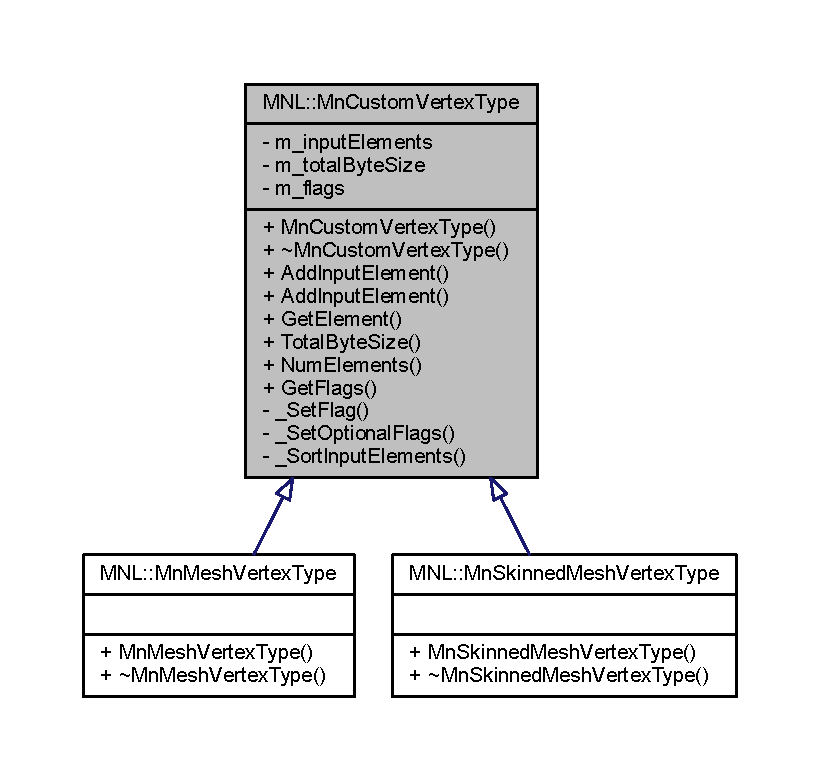
\includegraphics[width=350pt]{class_m_n_l_1_1_mn_custom_vertex_type__inherit__graph}
\end{center}
\end{figure}


M\+NL\+:\+:Mn\+Custom\+Vertex\+Type에 대한 협력 다이어그램\+:\nopagebreak
\begin{figure}[H]
\begin{center}
\leavevmode
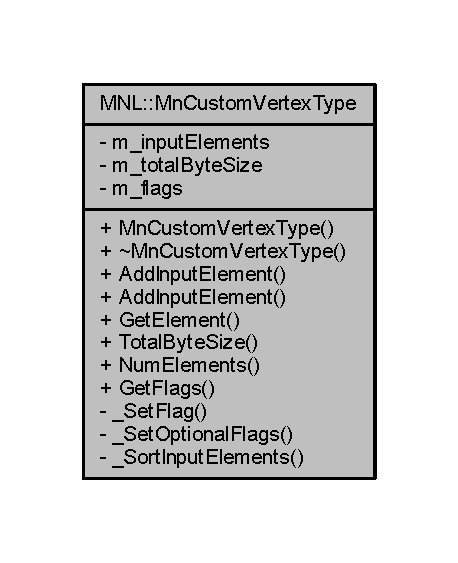
\includegraphics[width=220pt]{class_m_n_l_1_1_mn_custom_vertex_type__coll__graph}
\end{center}
\end{figure}
\subsection*{Public 멤버 함수}
\begin{DoxyCompactItemize}
\item 
\hyperlink{class_m_n_l_1_1_mn_custom_vertex_type_afb415522e4178413b715a31c15fe3b8e}{Mn\+Custom\+Vertex\+Type} ()
\item 
\hyperlink{class_m_n_l_1_1_mn_custom_vertex_type_a31288f3a89ead83464697fafe098f9e2}{$\sim$\+Mn\+Custom\+Vertex\+Type} ()
\item 
void \hyperlink{class_m_n_l_1_1_mn_custom_vertex_type_add19b1562c7ce78121b1e7ef79f8a614}{Add\+Input\+Element} (const \hyperlink{class_m_n_l_1_1_mn_input_element}{Mn\+Input\+Element} \&input\+Element)
\item 
void \hyperlink{class_m_n_l_1_1_mn_custom_vertex_type_af8dca54222b2c1e264ea7c1ec9ae8a18}{Add\+Input\+Element} (const \hyperlink{class_m_n_l_1_1_mn_input_element}{Mn\+Input\+Element} \&input\+Element, \hyperlink{namespace_m_n_l_a37da403537a061d6aaa45b7d30f29ac2}{M\+N\+\_\+\+C\+U\+S\+T\+O\+M\+\_\+\+V\+E\+R\+T\+E\+X\+\_\+\+F\+L\+AG} flags)
\item 
const \hyperlink{class_m_n_l_1_1_mn_input_element}{Mn\+Input\+Element} \& \hyperlink{class_m_n_l_1_1_mn_custom_vertex_type_ac7f43f6d20d9bf260b1afddd990b6056}{Get\+Element} (U\+I\+NT index) const
\item 
U\+I\+NT \hyperlink{class_m_n_l_1_1_mn_custom_vertex_type_a92e41bee4facb51cdef610ddb4292cd2}{Total\+Byte\+Size} () const
\item 
U\+I\+NT \hyperlink{class_m_n_l_1_1_mn_custom_vertex_type_afa660f1f13f78bcea74ee1440ba124f3}{Num\+Elements} () const
\item 
const U\+I\+N\+T16 \& \hyperlink{class_m_n_l_1_1_mn_custom_vertex_type_a1dbc7a044aaa7f1077d8338b4f510a21}{Get\+Flags} () const
\end{DoxyCompactItemize}
\subsection*{Private 멤버 함수}
\begin{DoxyCompactItemize}
\item 
void \hyperlink{class_m_n_l_1_1_mn_custom_vertex_type_a946914659f5fa5fcb9c880842d562a8f}{\+\_\+\+Set\+Flag} (const std\+::string \&semantic\+Name, U\+I\+NT index)
\item 
void \hyperlink{class_m_n_l_1_1_mn_custom_vertex_type_a0bda476a6929af13f8142df51808b3ae}{\+\_\+\+Set\+Optional\+Flags} (\hyperlink{namespace_m_n_l_a37da403537a061d6aaa45b7d30f29ac2}{M\+N\+\_\+\+C\+U\+S\+T\+O\+M\+\_\+\+V\+E\+R\+T\+E\+X\+\_\+\+F\+L\+AG} flags)
\item 
void \hyperlink{class_m_n_l_1_1_mn_custom_vertex_type_af969b32418900badbe331bf4190af1ee}{\+\_\+\+Sort\+Input\+Elements} ()
\end{DoxyCompactItemize}
\subsection*{Private 속성}
\begin{DoxyCompactItemize}
\item 
std\+::vector$<$ \hyperlink{class_m_n_l_1_1_mn_input_element}{Mn\+Input\+Element} $>$ \hyperlink{class_m_n_l_1_1_mn_custom_vertex_type_a965c3249b7bce95b3ef1cb5ce8c9e74e}{m\+\_\+input\+Elements}
\item 
U\+I\+NT \hyperlink{class_m_n_l_1_1_mn_custom_vertex_type_a07e3efae7a30c0c74665abf18426e336}{m\+\_\+total\+Byte\+Size}
\item 
U\+I\+N\+T16 \hyperlink{class_m_n_l_1_1_mn_custom_vertex_type_ac8677b700f6fec422fdbcc1071d24db6}{m\+\_\+flags}
\end{DoxyCompactItemize}


\subsection{상세한 설명}
Mn\+Custom\+Vertex holds vertex semantics, vertex structure. However the adding order, input elements are aligned by flags order. So user defined struct for a vertex should be ordered in P\+O\+S\+I\+T\+I\+O\+N-\/$>$N\+O\+R\+M\+A\+L-\/$>$T\+E\+X\+C\+O\+O\+R\+D-\/$>$O\+P\+T\+I\+O\+N\+AL 

Mn\+Custom\+Vertex\+Type.\+h 파일의 44 번째 라인에서 정의되었습니다.



\subsection{생성자 \& 소멸자 문서화}
\mbox{\Hypertarget{class_m_n_l_1_1_mn_custom_vertex_type_afb415522e4178413b715a31c15fe3b8e}\label{class_m_n_l_1_1_mn_custom_vertex_type_afb415522e4178413b715a31c15fe3b8e}} 
\index{M\+N\+L\+::\+Mn\+Custom\+Vertex\+Type@{M\+N\+L\+::\+Mn\+Custom\+Vertex\+Type}!Mn\+Custom\+Vertex\+Type@{Mn\+Custom\+Vertex\+Type}}
\index{Mn\+Custom\+Vertex\+Type@{Mn\+Custom\+Vertex\+Type}!M\+N\+L\+::\+Mn\+Custom\+Vertex\+Type@{M\+N\+L\+::\+Mn\+Custom\+Vertex\+Type}}
\subsubsection{\texorpdfstring{Mn\+Custom\+Vertex\+Type()}{MnCustomVertexType()}}
{\footnotesize\ttfamily Mn\+Custom\+Vertex\+Type\+::\+Mn\+Custom\+Vertex\+Type (\begin{DoxyParamCaption}{ }\end{DoxyParamCaption})}



Mn\+Custom\+Vertex\+Type.\+cpp 파일의 7 번째 라인에서 정의되었습니다.

\mbox{\Hypertarget{class_m_n_l_1_1_mn_custom_vertex_type_a31288f3a89ead83464697fafe098f9e2}\label{class_m_n_l_1_1_mn_custom_vertex_type_a31288f3a89ead83464697fafe098f9e2}} 
\index{M\+N\+L\+::\+Mn\+Custom\+Vertex\+Type@{M\+N\+L\+::\+Mn\+Custom\+Vertex\+Type}!````~Mn\+Custom\+Vertex\+Type@{$\sim$\+Mn\+Custom\+Vertex\+Type}}
\index{````~Mn\+Custom\+Vertex\+Type@{$\sim$\+Mn\+Custom\+Vertex\+Type}!M\+N\+L\+::\+Mn\+Custom\+Vertex\+Type@{M\+N\+L\+::\+Mn\+Custom\+Vertex\+Type}}
\subsubsection{\texorpdfstring{$\sim$\+Mn\+Custom\+Vertex\+Type()}{~MnCustomVertexType()}}
{\footnotesize\ttfamily Mn\+Custom\+Vertex\+Type\+::$\sim$\+Mn\+Custom\+Vertex\+Type (\begin{DoxyParamCaption}{ }\end{DoxyParamCaption})}



Mn\+Custom\+Vertex\+Type.\+cpp 파일의 12 번째 라인에서 정의되었습니다.



\subsection{멤버 함수 문서화}
\mbox{\Hypertarget{class_m_n_l_1_1_mn_custom_vertex_type_a946914659f5fa5fcb9c880842d562a8f}\label{class_m_n_l_1_1_mn_custom_vertex_type_a946914659f5fa5fcb9c880842d562a8f}} 
\index{M\+N\+L\+::\+Mn\+Custom\+Vertex\+Type@{M\+N\+L\+::\+Mn\+Custom\+Vertex\+Type}!\+\_\+\+Set\+Flag@{\+\_\+\+Set\+Flag}}
\index{\+\_\+\+Set\+Flag@{\+\_\+\+Set\+Flag}!M\+N\+L\+::\+Mn\+Custom\+Vertex\+Type@{M\+N\+L\+::\+Mn\+Custom\+Vertex\+Type}}
\subsubsection{\texorpdfstring{\+\_\+\+Set\+Flag()}{\_SetFlag()}}
{\footnotesize\ttfamily void Mn\+Custom\+Vertex\+Type\+::\+\_\+\+Set\+Flag (\begin{DoxyParamCaption}\item[{const std\+::string \&}]{semantic\+Name,  }\item[{U\+I\+NT}]{index }\end{DoxyParamCaption})\hspace{0.3cm}{\ttfamily [private]}}



Mn\+Custom\+Vertex\+Type.\+cpp 파일의 33 번째 라인에서 정의되었습니다.

\mbox{\Hypertarget{class_m_n_l_1_1_mn_custom_vertex_type_a0bda476a6929af13f8142df51808b3ae}\label{class_m_n_l_1_1_mn_custom_vertex_type_a0bda476a6929af13f8142df51808b3ae}} 
\index{M\+N\+L\+::\+Mn\+Custom\+Vertex\+Type@{M\+N\+L\+::\+Mn\+Custom\+Vertex\+Type}!\+\_\+\+Set\+Optional\+Flags@{\+\_\+\+Set\+Optional\+Flags}}
\index{\+\_\+\+Set\+Optional\+Flags@{\+\_\+\+Set\+Optional\+Flags}!M\+N\+L\+::\+Mn\+Custom\+Vertex\+Type@{M\+N\+L\+::\+Mn\+Custom\+Vertex\+Type}}
\subsubsection{\texorpdfstring{\+\_\+\+Set\+Optional\+Flags()}{\_SetOptionalFlags()}}
{\footnotesize\ttfamily void Mn\+Custom\+Vertex\+Type\+::\+\_\+\+Set\+Optional\+Flags (\begin{DoxyParamCaption}\item[{\hyperlink{namespace_m_n_l_a37da403537a061d6aaa45b7d30f29ac2}{M\+N\+\_\+\+C\+U\+S\+T\+O\+M\+\_\+\+V\+E\+R\+T\+E\+X\+\_\+\+F\+L\+AG}}]{flags }\end{DoxyParamCaption})\hspace{0.3cm}{\ttfamily [private]}}



Mn\+Custom\+Vertex\+Type.\+cpp 파일의 66 번째 라인에서 정의되었습니다.

\mbox{\Hypertarget{class_m_n_l_1_1_mn_custom_vertex_type_af969b32418900badbe331bf4190af1ee}\label{class_m_n_l_1_1_mn_custom_vertex_type_af969b32418900badbe331bf4190af1ee}} 
\index{M\+N\+L\+::\+Mn\+Custom\+Vertex\+Type@{M\+N\+L\+::\+Mn\+Custom\+Vertex\+Type}!\+\_\+\+Sort\+Input\+Elements@{\+\_\+\+Sort\+Input\+Elements}}
\index{\+\_\+\+Sort\+Input\+Elements@{\+\_\+\+Sort\+Input\+Elements}!M\+N\+L\+::\+Mn\+Custom\+Vertex\+Type@{M\+N\+L\+::\+Mn\+Custom\+Vertex\+Type}}
\subsubsection{\texorpdfstring{\+\_\+\+Sort\+Input\+Elements()}{\_SortInputElements()}}
{\footnotesize\ttfamily void Mn\+Custom\+Vertex\+Type\+::\+\_\+\+Sort\+Input\+Elements (\begin{DoxyParamCaption}{ }\end{DoxyParamCaption})\hspace{0.3cm}{\ttfamily [private]}}



Mn\+Custom\+Vertex\+Type.\+cpp 파일의 86 번째 라인에서 정의되었습니다.

\mbox{\Hypertarget{class_m_n_l_1_1_mn_custom_vertex_type_add19b1562c7ce78121b1e7ef79f8a614}\label{class_m_n_l_1_1_mn_custom_vertex_type_add19b1562c7ce78121b1e7ef79f8a614}} 
\index{M\+N\+L\+::\+Mn\+Custom\+Vertex\+Type@{M\+N\+L\+::\+Mn\+Custom\+Vertex\+Type}!Add\+Input\+Element@{Add\+Input\+Element}}
\index{Add\+Input\+Element@{Add\+Input\+Element}!M\+N\+L\+::\+Mn\+Custom\+Vertex\+Type@{M\+N\+L\+::\+Mn\+Custom\+Vertex\+Type}}
\subsubsection{\texorpdfstring{Add\+Input\+Element()}{AddInputElement()}\hspace{0.1cm}{\footnotesize\ttfamily [1/2]}}
{\footnotesize\ttfamily void Mn\+Custom\+Vertex\+Type\+::\+Add\+Input\+Element (\begin{DoxyParamCaption}\item[{const \hyperlink{class_m_n_l_1_1_mn_input_element}{Mn\+Input\+Element} \&}]{input\+Element }\end{DoxyParamCaption})}

Add a input element to description. input layout will be placed by adding order. 

Mn\+Custom\+Vertex\+Type.\+cpp 파일의 24 번째 라인에서 정의되었습니다.

\mbox{\Hypertarget{class_m_n_l_1_1_mn_custom_vertex_type_af8dca54222b2c1e264ea7c1ec9ae8a18}\label{class_m_n_l_1_1_mn_custom_vertex_type_af8dca54222b2c1e264ea7c1ec9ae8a18}} 
\index{M\+N\+L\+::\+Mn\+Custom\+Vertex\+Type@{M\+N\+L\+::\+Mn\+Custom\+Vertex\+Type}!Add\+Input\+Element@{Add\+Input\+Element}}
\index{Add\+Input\+Element@{Add\+Input\+Element}!M\+N\+L\+::\+Mn\+Custom\+Vertex\+Type@{M\+N\+L\+::\+Mn\+Custom\+Vertex\+Type}}
\subsubsection{\texorpdfstring{Add\+Input\+Element()}{AddInputElement()}\hspace{0.1cm}{\footnotesize\ttfamily [2/2]}}
{\footnotesize\ttfamily void Mn\+Custom\+Vertex\+Type\+::\+Add\+Input\+Element (\begin{DoxyParamCaption}\item[{const \hyperlink{class_m_n_l_1_1_mn_input_element}{Mn\+Input\+Element} \&}]{input\+Element,  }\item[{\hyperlink{namespace_m_n_l_a37da403537a061d6aaa45b7d30f29ac2}{M\+N\+\_\+\+C\+U\+S\+T\+O\+M\+\_\+\+V\+E\+R\+T\+E\+X\+\_\+\+F\+L\+AG}}]{flags }\end{DoxyParamCaption})}

Add a special-\/purpose-\/using element. 
\begin{DoxyParams}{매개변수}
{\em flags} & use only when there has a special purpose \\
\hline
\end{DoxyParams}


Mn\+Custom\+Vertex\+Type.\+cpp 파일의 16 번째 라인에서 정의되었습니다.

\mbox{\Hypertarget{class_m_n_l_1_1_mn_custom_vertex_type_ac7f43f6d20d9bf260b1afddd990b6056}\label{class_m_n_l_1_1_mn_custom_vertex_type_ac7f43f6d20d9bf260b1afddd990b6056}} 
\index{M\+N\+L\+::\+Mn\+Custom\+Vertex\+Type@{M\+N\+L\+::\+Mn\+Custom\+Vertex\+Type}!Get\+Element@{Get\+Element}}
\index{Get\+Element@{Get\+Element}!M\+N\+L\+::\+Mn\+Custom\+Vertex\+Type@{M\+N\+L\+::\+Mn\+Custom\+Vertex\+Type}}
\subsubsection{\texorpdfstring{Get\+Element()}{GetElement()}}
{\footnotesize\ttfamily const \hyperlink{class_m_n_l_1_1_mn_input_element}{Mn\+Input\+Element} \& Mn\+Custom\+Vertex\+Type\+::\+Get\+Element (\begin{DoxyParamCaption}\item[{U\+I\+NT}]{index }\end{DoxyParamCaption}) const}

Get a input element 
\begin{DoxyParams}{매개변수}
{\em index} & of the input elemenet \\
\hline
\end{DoxyParams}


Mn\+Custom\+Vertex\+Type.\+cpp 파일의 70 번째 라인에서 정의되었습니다.

\mbox{\Hypertarget{class_m_n_l_1_1_mn_custom_vertex_type_a1dbc7a044aaa7f1077d8338b4f510a21}\label{class_m_n_l_1_1_mn_custom_vertex_type_a1dbc7a044aaa7f1077d8338b4f510a21}} 
\index{M\+N\+L\+::\+Mn\+Custom\+Vertex\+Type@{M\+N\+L\+::\+Mn\+Custom\+Vertex\+Type}!Get\+Flags@{Get\+Flags}}
\index{Get\+Flags@{Get\+Flags}!M\+N\+L\+::\+Mn\+Custom\+Vertex\+Type@{M\+N\+L\+::\+Mn\+Custom\+Vertex\+Type}}
\subsubsection{\texorpdfstring{Get\+Flags()}{GetFlags()}}
{\footnotesize\ttfamily const U\+I\+N\+T16 \& Mn\+Custom\+Vertex\+Type\+::\+Get\+Flags (\begin{DoxyParamCaption}{ }\end{DoxyParamCaption}) const}



Mn\+Custom\+Vertex\+Type.\+cpp 파일의 82 번째 라인에서 정의되었습니다.

\mbox{\Hypertarget{class_m_n_l_1_1_mn_custom_vertex_type_afa660f1f13f78bcea74ee1440ba124f3}\label{class_m_n_l_1_1_mn_custom_vertex_type_afa660f1f13f78bcea74ee1440ba124f3}} 
\index{M\+N\+L\+::\+Mn\+Custom\+Vertex\+Type@{M\+N\+L\+::\+Mn\+Custom\+Vertex\+Type}!Num\+Elements@{Num\+Elements}}
\index{Num\+Elements@{Num\+Elements}!M\+N\+L\+::\+Mn\+Custom\+Vertex\+Type@{M\+N\+L\+::\+Mn\+Custom\+Vertex\+Type}}
\subsubsection{\texorpdfstring{Num\+Elements()}{NumElements()}}
{\footnotesize\ttfamily U\+I\+NT Mn\+Custom\+Vertex\+Type\+::\+Num\+Elements (\begin{DoxyParamCaption}{ }\end{DoxyParamCaption}) const}

\begin{DoxyReturn}{반환값}
count of input elements 
\end{DoxyReturn}


Mn\+Custom\+Vertex\+Type.\+cpp 파일의 78 번째 라인에서 정의되었습니다.

\mbox{\Hypertarget{class_m_n_l_1_1_mn_custom_vertex_type_a92e41bee4facb51cdef610ddb4292cd2}\label{class_m_n_l_1_1_mn_custom_vertex_type_a92e41bee4facb51cdef610ddb4292cd2}} 
\index{M\+N\+L\+::\+Mn\+Custom\+Vertex\+Type@{M\+N\+L\+::\+Mn\+Custom\+Vertex\+Type}!Total\+Byte\+Size@{Total\+Byte\+Size}}
\index{Total\+Byte\+Size@{Total\+Byte\+Size}!M\+N\+L\+::\+Mn\+Custom\+Vertex\+Type@{M\+N\+L\+::\+Mn\+Custom\+Vertex\+Type}}
\subsubsection{\texorpdfstring{Total\+Byte\+Size()}{TotalByteSize()}}
{\footnotesize\ttfamily U\+I\+NT Mn\+Custom\+Vertex\+Type\+::\+Total\+Byte\+Size (\begin{DoxyParamCaption}{ }\end{DoxyParamCaption}) const}

\begin{DoxyReturn}{반환값}
total byte size of whole input elements 
\end{DoxyReturn}


Mn\+Custom\+Vertex\+Type.\+cpp 파일의 74 번째 라인에서 정의되었습니다.



\subsection{멤버 데이터 문서화}
\mbox{\Hypertarget{class_m_n_l_1_1_mn_custom_vertex_type_ac8677b700f6fec422fdbcc1071d24db6}\label{class_m_n_l_1_1_mn_custom_vertex_type_ac8677b700f6fec422fdbcc1071d24db6}} 
\index{M\+N\+L\+::\+Mn\+Custom\+Vertex\+Type@{M\+N\+L\+::\+Mn\+Custom\+Vertex\+Type}!m\+\_\+flags@{m\+\_\+flags}}
\index{m\+\_\+flags@{m\+\_\+flags}!M\+N\+L\+::\+Mn\+Custom\+Vertex\+Type@{M\+N\+L\+::\+Mn\+Custom\+Vertex\+Type}}
\subsubsection{\texorpdfstring{m\+\_\+flags}{m\_flags}}
{\footnotesize\ttfamily U\+I\+N\+T16 M\+N\+L\+::\+Mn\+Custom\+Vertex\+Type\+::m\+\_\+flags\hspace{0.3cm}{\ttfamily [private]}}

0x F F F F P\+OS N\+O\+RM T\+EX O\+PT 

Mn\+Custom\+Vertex\+Type.\+h 파일의 95 번째 라인에서 정의되었습니다.

\mbox{\Hypertarget{class_m_n_l_1_1_mn_custom_vertex_type_a965c3249b7bce95b3ef1cb5ce8c9e74e}\label{class_m_n_l_1_1_mn_custom_vertex_type_a965c3249b7bce95b3ef1cb5ce8c9e74e}} 
\index{M\+N\+L\+::\+Mn\+Custom\+Vertex\+Type@{M\+N\+L\+::\+Mn\+Custom\+Vertex\+Type}!m\+\_\+input\+Elements@{m\+\_\+input\+Elements}}
\index{m\+\_\+input\+Elements@{m\+\_\+input\+Elements}!M\+N\+L\+::\+Mn\+Custom\+Vertex\+Type@{M\+N\+L\+::\+Mn\+Custom\+Vertex\+Type}}
\subsubsection{\texorpdfstring{m\+\_\+input\+Elements}{m\_inputElements}}
{\footnotesize\ttfamily std\+::vector$<$\hyperlink{class_m_n_l_1_1_mn_input_element}{Mn\+Input\+Element}$>$ M\+N\+L\+::\+Mn\+Custom\+Vertex\+Type\+::m\+\_\+input\+Elements\hspace{0.3cm}{\ttfamily [private]}}



Mn\+Custom\+Vertex\+Type.\+h 파일의 89 번째 라인에서 정의되었습니다.

\mbox{\Hypertarget{class_m_n_l_1_1_mn_custom_vertex_type_a07e3efae7a30c0c74665abf18426e336}\label{class_m_n_l_1_1_mn_custom_vertex_type_a07e3efae7a30c0c74665abf18426e336}} 
\index{M\+N\+L\+::\+Mn\+Custom\+Vertex\+Type@{M\+N\+L\+::\+Mn\+Custom\+Vertex\+Type}!m\+\_\+total\+Byte\+Size@{m\+\_\+total\+Byte\+Size}}
\index{m\+\_\+total\+Byte\+Size@{m\+\_\+total\+Byte\+Size}!M\+N\+L\+::\+Mn\+Custom\+Vertex\+Type@{M\+N\+L\+::\+Mn\+Custom\+Vertex\+Type}}
\subsubsection{\texorpdfstring{m\+\_\+total\+Byte\+Size}{m\_totalByteSize}}
{\footnotesize\ttfamily U\+I\+NT M\+N\+L\+::\+Mn\+Custom\+Vertex\+Type\+::m\+\_\+total\+Byte\+Size\hspace{0.3cm}{\ttfamily [private]}}



Mn\+Custom\+Vertex\+Type.\+h 파일의 90 번째 라인에서 정의되었습니다.



이 클래스에 대한 문서화 페이지는 다음의 파일들로부터 생성되었습니다.\+:\begin{DoxyCompactItemize}
\item 
Core/\hyperlink{_mn_custom_vertex_type_8h}{Mn\+Custom\+Vertex\+Type.\+h}\item 
Core/\hyperlink{_mn_custom_vertex_type_8cpp}{Mn\+Custom\+Vertex\+Type.\+cpp}\end{DoxyCompactItemize}

\hypertarget{class_m_n_l_1_1_mn_d3_d_device}{}\section{M\+NL\+:\+:Mn\+D3\+D\+Device 클래스 참조}
\label{class_m_n_l_1_1_mn_d3_d_device}\index{M\+N\+L\+::\+Mn\+D3\+D\+Device@{M\+N\+L\+::\+Mn\+D3\+D\+Device}}


D\+Irect\+X11 디바이스와 디바이스 컨텍스트를 생성, 관리한다.  




{\ttfamily \#include $<$Mn\+D3\+D\+Device.\+h$>$}



M\+NL\+:\+:Mn\+D3\+D\+Device에 대한 협력 다이어그램\+:\nopagebreak
\begin{figure}[H]
\begin{center}
\leavevmode
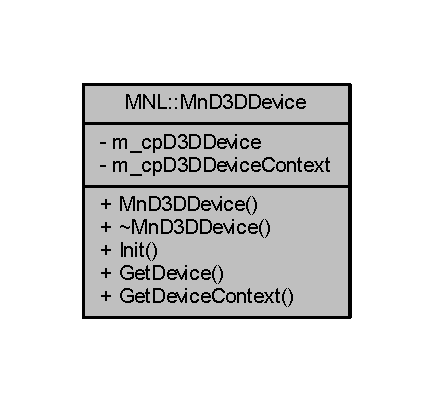
\includegraphics[width=208pt]{class_m_n_l_1_1_mn_d3_d_device__coll__graph}
\end{center}
\end{figure}
\subsection*{Public 멤버 함수}
\begin{DoxyCompactItemize}
\item 
\hyperlink{class_m_n_l_1_1_mn_d3_d_device_a73cd90c6f415ae81a05cdb11303c1d51}{Mn\+D3\+D\+Device} ()
\item 
\hyperlink{class_m_n_l_1_1_mn_d3_d_device_abdd98dae30351ff08198db0f97f6ffd9}{$\sim$\+Mn\+D3\+D\+Device} ()
\item 
H\+R\+E\+S\+U\+LT \hyperlink{class_m_n_l_1_1_mn_d3_d_device_aada86462878af0f620871fc4b9836edc}{Init} (const \hyperlink{class_m_n_l_1_1_mn_hardware}{Mn\+Hardware} \&hardware\+Info, bool use\+Default\+Adapter)
\begin{DoxyCompactList}\small\item\em D3\+D\+Device, D3\+D\+Device\+Context 인터페이스를 생성, 초기화 한다. \end{DoxyCompactList}\item 
\hyperlink{namespace_m_n_l_a1eec210db8f309a4a9ac0d9658784c31}{C\+P\+D3\+D\+Device} \hyperlink{class_m_n_l_1_1_mn_d3_d_device_a0143842e6feb74a12d6849914c1beb46}{Get\+Device} () const
\begin{DoxyCompactList}\small\item\em D3\+D\+Device 인터페이스를 반환한다. \end{DoxyCompactList}\item 
\hyperlink{namespace_m_n_l_aab3aabb6c9360e44ddc8b0bb563c2107}{C\+P\+D3\+D\+Device\+Context} \hyperlink{class_m_n_l_1_1_mn_d3_d_device_aef186783679d2fd2ad183cca0bcf9299}{Get\+Device\+Context} () const
\begin{DoxyCompactList}\small\item\em D3\+D\+Device\+Context 인터페이스를 반환한다. \end{DoxyCompactList}\end{DoxyCompactItemize}
\subsection*{Private 속성}
\begin{DoxyCompactItemize}
\item 
\hyperlink{namespace_m_n_l_a1eec210db8f309a4a9ac0d9658784c31}{C\+P\+D3\+D\+Device} \hyperlink{class_m_n_l_1_1_mn_d3_d_device_a799a2d8f1c5b2c3fdc2e003952279a4f}{m\+\_\+cp\+D3\+D\+Device}
\begin{DoxyCompactList}\small\item\em D3\+Device 인터페이스 \end{DoxyCompactList}\item 
\hyperlink{namespace_m_n_l_aab3aabb6c9360e44ddc8b0bb563c2107}{C\+P\+D3\+D\+Device\+Context} \hyperlink{class_m_n_l_1_1_mn_d3_d_device_a718aa02b1c1e40c4f3b91b6a3c68eff2}{m\+\_\+cp\+D3\+D\+Device\+Context}
\end{DoxyCompactItemize}


\subsection{상세한 설명}
D\+Irect\+X11 디바이스와 디바이스 컨텍스트를 생성, 관리한다. 

\begin{DoxyAuthor}{작성자}
Akssus 
\end{DoxyAuthor}
\hypertarget{class_m_n_l_1_1_mn_video_adapter_개요}{}\subsection{개요}\label{class_m_n_l_1_1_mn_video_adapter_개요}
Mn\+D3\+D\+Device를 초기화 하기 위해선 초기화된 \hyperlink{class_m_n_l_1_1_mn_hardware}{Mn\+Hardware} 객체가 필요하다. ~\newline
Mn\+D3\+D\+Device는 \hyperlink{class_m_n_l_1_1_mn_hardware}{Mn\+Hardware} 객체로부터 비디오 어댑터의 인터페이스를 얻어와 D3\+D\+Device 인터페이스와 D3\+D\+Device\+Context 인터페이스를 생성한다. ~\newline
초기화 된 Mn\+D3\+D\+Device는 \hyperlink{class_m_n_l_1_1_mn_render_a_p_i}{Mn\+Render\+A\+PI} 클래스에서 비디오 어댑터 장치와 상호작용 하는데 사용된다. 

Mn\+D3\+D\+Device.\+h 파일의 18 번째 라인에서 정의되었습니다.



\subsection{생성자 \& 소멸자 문서화}
\mbox{\Hypertarget{class_m_n_l_1_1_mn_d3_d_device_a73cd90c6f415ae81a05cdb11303c1d51}\label{class_m_n_l_1_1_mn_d3_d_device_a73cd90c6f415ae81a05cdb11303c1d51}} 
\index{M\+N\+L\+::\+Mn\+D3\+D\+Device@{M\+N\+L\+::\+Mn\+D3\+D\+Device}!Mn\+D3\+D\+Device@{Mn\+D3\+D\+Device}}
\index{Mn\+D3\+D\+Device@{Mn\+D3\+D\+Device}!M\+N\+L\+::\+Mn\+D3\+D\+Device@{M\+N\+L\+::\+Mn\+D3\+D\+Device}}
\subsubsection{\texorpdfstring{Mn\+D3\+D\+Device()}{MnD3DDevice()}}
{\footnotesize\ttfamily Mn\+D3\+D\+Device\+::\+Mn\+D3\+D\+Device (\begin{DoxyParamCaption}{ }\end{DoxyParamCaption})}



Mn\+D3\+D\+Device.\+cpp 파일의 6 번째 라인에서 정의되었습니다.

\mbox{\Hypertarget{class_m_n_l_1_1_mn_d3_d_device_abdd98dae30351ff08198db0f97f6ffd9}\label{class_m_n_l_1_1_mn_d3_d_device_abdd98dae30351ff08198db0f97f6ffd9}} 
\index{M\+N\+L\+::\+Mn\+D3\+D\+Device@{M\+N\+L\+::\+Mn\+D3\+D\+Device}!````~Mn\+D3\+D\+Device@{$\sim$\+Mn\+D3\+D\+Device}}
\index{````~Mn\+D3\+D\+Device@{$\sim$\+Mn\+D3\+D\+Device}!M\+N\+L\+::\+Mn\+D3\+D\+Device@{M\+N\+L\+::\+Mn\+D3\+D\+Device}}
\subsubsection{\texorpdfstring{$\sim$\+Mn\+D3\+D\+Device()}{~MnD3DDevice()}}
{\footnotesize\ttfamily Mn\+D3\+D\+Device\+::$\sim$\+Mn\+D3\+D\+Device (\begin{DoxyParamCaption}{ }\end{DoxyParamCaption})}



Mn\+D3\+D\+Device.\+cpp 파일의 11 번째 라인에서 정의되었습니다.



\subsection{멤버 함수 문서화}
\mbox{\Hypertarget{class_m_n_l_1_1_mn_d3_d_device_a0143842e6feb74a12d6849914c1beb46}\label{class_m_n_l_1_1_mn_d3_d_device_a0143842e6feb74a12d6849914c1beb46}} 
\index{M\+N\+L\+::\+Mn\+D3\+D\+Device@{M\+N\+L\+::\+Mn\+D3\+D\+Device}!Get\+Device@{Get\+Device}}
\index{Get\+Device@{Get\+Device}!M\+N\+L\+::\+Mn\+D3\+D\+Device@{M\+N\+L\+::\+Mn\+D3\+D\+Device}}
\subsubsection{\texorpdfstring{Get\+Device()}{GetDevice()}}
{\footnotesize\ttfamily \hyperlink{namespace_m_n_l_a1eec210db8f309a4a9ac0d9658784c31}{C\+P\+D3\+D\+Device} Mn\+D3\+D\+Device\+::\+Get\+Device (\begin{DoxyParamCaption}{ }\end{DoxyParamCaption}) const}



D3\+D\+Device 인터페이스를 반환한다. 



Mn\+D3\+D\+Device.\+cpp 파일의 47 번째 라인에서 정의되었습니다.

\mbox{\Hypertarget{class_m_n_l_1_1_mn_d3_d_device_aef186783679d2fd2ad183cca0bcf9299}\label{class_m_n_l_1_1_mn_d3_d_device_aef186783679d2fd2ad183cca0bcf9299}} 
\index{M\+N\+L\+::\+Mn\+D3\+D\+Device@{M\+N\+L\+::\+Mn\+D3\+D\+Device}!Get\+Device\+Context@{Get\+Device\+Context}}
\index{Get\+Device\+Context@{Get\+Device\+Context}!M\+N\+L\+::\+Mn\+D3\+D\+Device@{M\+N\+L\+::\+Mn\+D3\+D\+Device}}
\subsubsection{\texorpdfstring{Get\+Device\+Context()}{GetDeviceContext()}}
{\footnotesize\ttfamily \hyperlink{namespace_m_n_l_aab3aabb6c9360e44ddc8b0bb563c2107}{C\+P\+D3\+D\+Device\+Context} Mn\+D3\+D\+Device\+::\+Get\+Device\+Context (\begin{DoxyParamCaption}{ }\end{DoxyParamCaption}) const}



D3\+D\+Device\+Context 인터페이스를 반환한다. 



Mn\+D3\+D\+Device.\+cpp 파일의 51 번째 라인에서 정의되었습니다.

\mbox{\Hypertarget{class_m_n_l_1_1_mn_d3_d_device_aada86462878af0f620871fc4b9836edc}\label{class_m_n_l_1_1_mn_d3_d_device_aada86462878af0f620871fc4b9836edc}} 
\index{M\+N\+L\+::\+Mn\+D3\+D\+Device@{M\+N\+L\+::\+Mn\+D3\+D\+Device}!Init@{Init}}
\index{Init@{Init}!M\+N\+L\+::\+Mn\+D3\+D\+Device@{M\+N\+L\+::\+Mn\+D3\+D\+Device}}
\subsubsection{\texorpdfstring{Init()}{Init()}}
{\footnotesize\ttfamily H\+R\+E\+S\+U\+LT Mn\+D3\+D\+Device\+::\+Init (\begin{DoxyParamCaption}\item[{const \hyperlink{class_m_n_l_1_1_mn_hardware}{Mn\+Hardware} \&}]{hardware\+Info,  }\item[{bool}]{use\+Default\+Adapter }\end{DoxyParamCaption})}



D3\+D\+Device, D3\+D\+Device\+Context 인터페이스를 생성, 초기화 한다. 


\begin{DoxyParams}{매개변수}
{\em use\+Default\+Adapter} & 디폴트 비디오 어댑터 사용 여부. \\
\hline
\end{DoxyParams}
\begin{DoxyReturn}{반환값}
초기화 성공 여부. 
\end{DoxyReturn}
\begin{DoxyWarning}{경고}
현재 use\+Default\+Adapter 값과 관계 없이 디폴트 값으로 초기화 된다. 
\end{DoxyWarning}


Mn\+D3\+D\+Device.\+cpp 파일의 15 번째 라인에서 정의되었습니다.



\subsection{멤버 데이터 문서화}
\mbox{\Hypertarget{class_m_n_l_1_1_mn_d3_d_device_a799a2d8f1c5b2c3fdc2e003952279a4f}\label{class_m_n_l_1_1_mn_d3_d_device_a799a2d8f1c5b2c3fdc2e003952279a4f}} 
\index{M\+N\+L\+::\+Mn\+D3\+D\+Device@{M\+N\+L\+::\+Mn\+D3\+D\+Device}!m\+\_\+cp\+D3\+D\+Device@{m\+\_\+cp\+D3\+D\+Device}}
\index{m\+\_\+cp\+D3\+D\+Device@{m\+\_\+cp\+D3\+D\+Device}!M\+N\+L\+::\+Mn\+D3\+D\+Device@{M\+N\+L\+::\+Mn\+D3\+D\+Device}}
\subsubsection{\texorpdfstring{m\+\_\+cp\+D3\+D\+Device}{m\_cpD3DDevice}}
{\footnotesize\ttfamily \hyperlink{namespace_m_n_l_a1eec210db8f309a4a9ac0d9658784c31}{C\+P\+D3\+D\+Device} M\+N\+L\+::\+Mn\+D3\+D\+Device\+::m\+\_\+cp\+D3\+D\+Device\hspace{0.3cm}{\ttfamily [private]}}



D3\+Device 인터페이스 



Mn\+D3\+D\+Device.\+h 파일의 41 번째 라인에서 정의되었습니다.

\mbox{\Hypertarget{class_m_n_l_1_1_mn_d3_d_device_a718aa02b1c1e40c4f3b91b6a3c68eff2}\label{class_m_n_l_1_1_mn_d3_d_device_a718aa02b1c1e40c4f3b91b6a3c68eff2}} 
\index{M\+N\+L\+::\+Mn\+D3\+D\+Device@{M\+N\+L\+::\+Mn\+D3\+D\+Device}!m\+\_\+cp\+D3\+D\+Device\+Context@{m\+\_\+cp\+D3\+D\+Device\+Context}}
\index{m\+\_\+cp\+D3\+D\+Device\+Context@{m\+\_\+cp\+D3\+D\+Device\+Context}!M\+N\+L\+::\+Mn\+D3\+D\+Device@{M\+N\+L\+::\+Mn\+D3\+D\+Device}}
\subsubsection{\texorpdfstring{m\+\_\+cp\+D3\+D\+Device\+Context}{m\_cpD3DDeviceContext}}
{\footnotesize\ttfamily \hyperlink{namespace_m_n_l_aab3aabb6c9360e44ddc8b0bb563c2107}{C\+P\+D3\+D\+Device\+Context} M\+N\+L\+::\+Mn\+D3\+D\+Device\+::m\+\_\+cp\+D3\+D\+Device\+Context\hspace{0.3cm}{\ttfamily [private]}}



Mn\+D3\+D\+Device.\+h 파일의 42 번째 라인에서 정의되었습니다.



이 클래스에 대한 문서화 페이지는 다음의 파일들로부터 생성되었습니다.\+:\begin{DoxyCompactItemize}
\item 
Core/\hyperlink{_mn_d3_d_device_8h}{Mn\+D3\+D\+Device.\+h}\item 
Core/\hyperlink{_mn_d3_d_device_8cpp}{Mn\+D3\+D\+Device.\+cpp}\end{DoxyCompactItemize}

\hypertarget{class_m_n_l_1_1_mn_depth_stencil_buffer}{}\section{M\+NL\+:\+:Mn\+Depth\+Stencil\+Buffer 클래스 참조}
\label{class_m_n_l_1_1_mn_depth_stencil_buffer}\index{M\+N\+L\+::\+Mn\+Depth\+Stencil\+Buffer@{M\+N\+L\+::\+Mn\+Depth\+Stencil\+Buffer}}


{\ttfamily \#include $<$Mn\+Depth\+Stencil\+Buffer.\+h$>$}



M\+NL\+:\+:Mn\+Depth\+Stencil\+Buffer에 대한 협력 다이어그램\+:\nopagebreak
\begin{figure}[H]
\begin{center}
\leavevmode
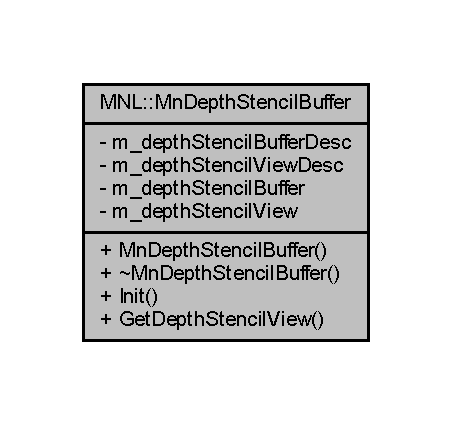
\includegraphics[width=217pt]{class_m_n_l_1_1_mn_depth_stencil_buffer__coll__graph}
\end{center}
\end{figure}
\subsection*{Public 멤버 함수}
\begin{DoxyCompactItemize}
\item 
\hyperlink{class_m_n_l_1_1_mn_depth_stencil_buffer_a62c99b992fdd488bbcedee12e377e09f}{Mn\+Depth\+Stencil\+Buffer} ()
\item 
\hyperlink{class_m_n_l_1_1_mn_depth_stencil_buffer_a887ad94ae7dbf34b1599f63874e42433}{$\sim$\+Mn\+Depth\+Stencil\+Buffer} ()
\item 
H\+R\+E\+S\+U\+LT \hyperlink{class_m_n_l_1_1_mn_depth_stencil_buffer_a5cbabb78041c31d65ff6204aa733fa44}{Init} (const \hyperlink{namespace_m_n_l_a1eec210db8f309a4a9ac0d9658784c31}{C\+P\+D3\+D\+Device} cp\+Device, U\+I\+NT width, U\+I\+NT height)
\item 
const \hyperlink{namespace_m_n_l_a12b3c209d76ede855300e637f4192a04}{C\+P\+D3\+D\+Depth\+Stencil\+View} \& \hyperlink{class_m_n_l_1_1_mn_depth_stencil_buffer_aa05ba43eb3a290433969f2ca7972bc00}{Get\+Depth\+Stencil\+View} () const
\end{DoxyCompactItemize}
\subsection*{Private 속성}
\begin{DoxyCompactItemize}
\item 
D3\+D11\+\_\+\+T\+E\+X\+T\+U\+R\+E2\+D\+\_\+\+D\+E\+SC \hyperlink{class_m_n_l_1_1_mn_depth_stencil_buffer_a35c7153f9064c5d503391b546fe41437}{m\+\_\+depth\+Stencil\+Buffer\+Desc}
\item 
D3\+D11\+\_\+\+D\+E\+P\+T\+H\+\_\+\+S\+T\+E\+N\+C\+I\+L\+\_\+\+V\+I\+E\+W\+\_\+\+D\+E\+SC \hyperlink{class_m_n_l_1_1_mn_depth_stencil_buffer_a30ce2c7cebdd1db6c6a08ae22d7f9269}{m\+\_\+depth\+Stencil\+View\+Desc}
\item 
\hyperlink{namespace_m_n_l_addb538e1cbd1f443e6db5e6312487c51}{C\+P\+D3\+D\+Texture2D} \hyperlink{class_m_n_l_1_1_mn_depth_stencil_buffer_ae995fe33e73c061329841ca2e1fd1c0d}{m\+\_\+depth\+Stencil\+Buffer}
\item 
\hyperlink{namespace_m_n_l_a12b3c209d76ede855300e637f4192a04}{C\+P\+D3\+D\+Depth\+Stencil\+View} \hyperlink{class_m_n_l_1_1_mn_depth_stencil_buffer_a0be4d4b37417df8478e891b471bdd270}{m\+\_\+depth\+Stencil\+View}
\end{DoxyCompactItemize}


\subsection{상세한 설명}


Mn\+Depth\+Stencil\+Buffer.\+h 파일의 7 번째 라인에서 정의되었습니다.



\subsection{생성자 \& 소멸자 문서화}
\mbox{\Hypertarget{class_m_n_l_1_1_mn_depth_stencil_buffer_a62c99b992fdd488bbcedee12e377e09f}\label{class_m_n_l_1_1_mn_depth_stencil_buffer_a62c99b992fdd488bbcedee12e377e09f}} 
\index{M\+N\+L\+::\+Mn\+Depth\+Stencil\+Buffer@{M\+N\+L\+::\+Mn\+Depth\+Stencil\+Buffer}!Mn\+Depth\+Stencil\+Buffer@{Mn\+Depth\+Stencil\+Buffer}}
\index{Mn\+Depth\+Stencil\+Buffer@{Mn\+Depth\+Stencil\+Buffer}!M\+N\+L\+::\+Mn\+Depth\+Stencil\+Buffer@{M\+N\+L\+::\+Mn\+Depth\+Stencil\+Buffer}}
\subsubsection{\texorpdfstring{Mn\+Depth\+Stencil\+Buffer()}{MnDepthStencilBuffer()}}
{\footnotesize\ttfamily Mn\+Depth\+Stencil\+Buffer\+::\+Mn\+Depth\+Stencil\+Buffer (\begin{DoxyParamCaption}{ }\end{DoxyParamCaption})}



Mn\+Depth\+Stencil\+Buffer.\+cpp 파일의 6 번째 라인에서 정의되었습니다.

\mbox{\Hypertarget{class_m_n_l_1_1_mn_depth_stencil_buffer_a887ad94ae7dbf34b1599f63874e42433}\label{class_m_n_l_1_1_mn_depth_stencil_buffer_a887ad94ae7dbf34b1599f63874e42433}} 
\index{M\+N\+L\+::\+Mn\+Depth\+Stencil\+Buffer@{M\+N\+L\+::\+Mn\+Depth\+Stencil\+Buffer}!````~Mn\+Depth\+Stencil\+Buffer@{$\sim$\+Mn\+Depth\+Stencil\+Buffer}}
\index{````~Mn\+Depth\+Stencil\+Buffer@{$\sim$\+Mn\+Depth\+Stencil\+Buffer}!M\+N\+L\+::\+Mn\+Depth\+Stencil\+Buffer@{M\+N\+L\+::\+Mn\+Depth\+Stencil\+Buffer}}
\subsubsection{\texorpdfstring{$\sim$\+Mn\+Depth\+Stencil\+Buffer()}{~MnDepthStencilBuffer()}}
{\footnotesize\ttfamily Mn\+Depth\+Stencil\+Buffer\+::$\sim$\+Mn\+Depth\+Stencil\+Buffer (\begin{DoxyParamCaption}{ }\end{DoxyParamCaption})}



Mn\+Depth\+Stencil\+Buffer.\+cpp 파일의 13 번째 라인에서 정의되었습니다.



\subsection{멤버 함수 문서화}
\mbox{\Hypertarget{class_m_n_l_1_1_mn_depth_stencil_buffer_aa05ba43eb3a290433969f2ca7972bc00}\label{class_m_n_l_1_1_mn_depth_stencil_buffer_aa05ba43eb3a290433969f2ca7972bc00}} 
\index{M\+N\+L\+::\+Mn\+Depth\+Stencil\+Buffer@{M\+N\+L\+::\+Mn\+Depth\+Stencil\+Buffer}!Get\+Depth\+Stencil\+View@{Get\+Depth\+Stencil\+View}}
\index{Get\+Depth\+Stencil\+View@{Get\+Depth\+Stencil\+View}!M\+N\+L\+::\+Mn\+Depth\+Stencil\+Buffer@{M\+N\+L\+::\+Mn\+Depth\+Stencil\+Buffer}}
\subsubsection{\texorpdfstring{Get\+Depth\+Stencil\+View()}{GetDepthStencilView()}}
{\footnotesize\ttfamily const \hyperlink{namespace_m_n_l_a12b3c209d76ede855300e637f4192a04}{C\+P\+D3\+D\+Depth\+Stencil\+View} \& Mn\+Depth\+Stencil\+Buffer\+::\+Get\+Depth\+Stencil\+View (\begin{DoxyParamCaption}{ }\end{DoxyParamCaption}) const}



Mn\+Depth\+Stencil\+Buffer.\+cpp 파일의 56 번째 라인에서 정의되었습니다.

\mbox{\Hypertarget{class_m_n_l_1_1_mn_depth_stencil_buffer_a5cbabb78041c31d65ff6204aa733fa44}\label{class_m_n_l_1_1_mn_depth_stencil_buffer_a5cbabb78041c31d65ff6204aa733fa44}} 
\index{M\+N\+L\+::\+Mn\+Depth\+Stencil\+Buffer@{M\+N\+L\+::\+Mn\+Depth\+Stencil\+Buffer}!Init@{Init}}
\index{Init@{Init}!M\+N\+L\+::\+Mn\+Depth\+Stencil\+Buffer@{M\+N\+L\+::\+Mn\+Depth\+Stencil\+Buffer}}
\subsubsection{\texorpdfstring{Init()}{Init()}}
{\footnotesize\ttfamily H\+R\+E\+S\+U\+LT Mn\+Depth\+Stencil\+Buffer\+::\+Init (\begin{DoxyParamCaption}\item[{const \hyperlink{namespace_m_n_l_a1eec210db8f309a4a9ac0d9658784c31}{C\+P\+D3\+D\+Device}}]{cp\+Device,  }\item[{U\+I\+NT}]{width,  }\item[{U\+I\+NT}]{height }\end{DoxyParamCaption})}



Mn\+Depth\+Stencil\+Buffer.\+cpp 파일의 17 번째 라인에서 정의되었습니다.



\subsection{멤버 데이터 문서화}
\mbox{\Hypertarget{class_m_n_l_1_1_mn_depth_stencil_buffer_ae995fe33e73c061329841ca2e1fd1c0d}\label{class_m_n_l_1_1_mn_depth_stencil_buffer_ae995fe33e73c061329841ca2e1fd1c0d}} 
\index{M\+N\+L\+::\+Mn\+Depth\+Stencil\+Buffer@{M\+N\+L\+::\+Mn\+Depth\+Stencil\+Buffer}!m\+\_\+depth\+Stencil\+Buffer@{m\+\_\+depth\+Stencil\+Buffer}}
\index{m\+\_\+depth\+Stencil\+Buffer@{m\+\_\+depth\+Stencil\+Buffer}!M\+N\+L\+::\+Mn\+Depth\+Stencil\+Buffer@{M\+N\+L\+::\+Mn\+Depth\+Stencil\+Buffer}}
\subsubsection{\texorpdfstring{m\+\_\+depth\+Stencil\+Buffer}{m\_depthStencilBuffer}}
{\footnotesize\ttfamily \hyperlink{namespace_m_n_l_addb538e1cbd1f443e6db5e6312487c51}{C\+P\+D3\+D\+Texture2D} M\+N\+L\+::\+Mn\+Depth\+Stencil\+Buffer\+::m\+\_\+depth\+Stencil\+Buffer\hspace{0.3cm}{\ttfamily [private]}}



Mn\+Depth\+Stencil\+Buffer.\+h 파일의 19 번째 라인에서 정의되었습니다.

\mbox{\Hypertarget{class_m_n_l_1_1_mn_depth_stencil_buffer_a35c7153f9064c5d503391b546fe41437}\label{class_m_n_l_1_1_mn_depth_stencil_buffer_a35c7153f9064c5d503391b546fe41437}} 
\index{M\+N\+L\+::\+Mn\+Depth\+Stencil\+Buffer@{M\+N\+L\+::\+Mn\+Depth\+Stencil\+Buffer}!m\+\_\+depth\+Stencil\+Buffer\+Desc@{m\+\_\+depth\+Stencil\+Buffer\+Desc}}
\index{m\+\_\+depth\+Stencil\+Buffer\+Desc@{m\+\_\+depth\+Stencil\+Buffer\+Desc}!M\+N\+L\+::\+Mn\+Depth\+Stencil\+Buffer@{M\+N\+L\+::\+Mn\+Depth\+Stencil\+Buffer}}
\subsubsection{\texorpdfstring{m\+\_\+depth\+Stencil\+Buffer\+Desc}{m\_depthStencilBufferDesc}}
{\footnotesize\ttfamily D3\+D11\+\_\+\+T\+E\+X\+T\+U\+R\+E2\+D\+\_\+\+D\+E\+SC M\+N\+L\+::\+Mn\+Depth\+Stencil\+Buffer\+::m\+\_\+depth\+Stencil\+Buffer\+Desc\hspace{0.3cm}{\ttfamily [private]}}



Mn\+Depth\+Stencil\+Buffer.\+h 파일의 17 번째 라인에서 정의되었습니다.

\mbox{\Hypertarget{class_m_n_l_1_1_mn_depth_stencil_buffer_a0be4d4b37417df8478e891b471bdd270}\label{class_m_n_l_1_1_mn_depth_stencil_buffer_a0be4d4b37417df8478e891b471bdd270}} 
\index{M\+N\+L\+::\+Mn\+Depth\+Stencil\+Buffer@{M\+N\+L\+::\+Mn\+Depth\+Stencil\+Buffer}!m\+\_\+depth\+Stencil\+View@{m\+\_\+depth\+Stencil\+View}}
\index{m\+\_\+depth\+Stencil\+View@{m\+\_\+depth\+Stencil\+View}!M\+N\+L\+::\+Mn\+Depth\+Stencil\+Buffer@{M\+N\+L\+::\+Mn\+Depth\+Stencil\+Buffer}}
\subsubsection{\texorpdfstring{m\+\_\+depth\+Stencil\+View}{m\_depthStencilView}}
{\footnotesize\ttfamily \hyperlink{namespace_m_n_l_a12b3c209d76ede855300e637f4192a04}{C\+P\+D3\+D\+Depth\+Stencil\+View} M\+N\+L\+::\+Mn\+Depth\+Stencil\+Buffer\+::m\+\_\+depth\+Stencil\+View\hspace{0.3cm}{\ttfamily [private]}}



Mn\+Depth\+Stencil\+Buffer.\+h 파일의 20 번째 라인에서 정의되었습니다.

\mbox{\Hypertarget{class_m_n_l_1_1_mn_depth_stencil_buffer_a30ce2c7cebdd1db6c6a08ae22d7f9269}\label{class_m_n_l_1_1_mn_depth_stencil_buffer_a30ce2c7cebdd1db6c6a08ae22d7f9269}} 
\index{M\+N\+L\+::\+Mn\+Depth\+Stencil\+Buffer@{M\+N\+L\+::\+Mn\+Depth\+Stencil\+Buffer}!m\+\_\+depth\+Stencil\+View\+Desc@{m\+\_\+depth\+Stencil\+View\+Desc}}
\index{m\+\_\+depth\+Stencil\+View\+Desc@{m\+\_\+depth\+Stencil\+View\+Desc}!M\+N\+L\+::\+Mn\+Depth\+Stencil\+Buffer@{M\+N\+L\+::\+Mn\+Depth\+Stencil\+Buffer}}
\subsubsection{\texorpdfstring{m\+\_\+depth\+Stencil\+View\+Desc}{m\_depthStencilViewDesc}}
{\footnotesize\ttfamily D3\+D11\+\_\+\+D\+E\+P\+T\+H\+\_\+\+S\+T\+E\+N\+C\+I\+L\+\_\+\+V\+I\+E\+W\+\_\+\+D\+E\+SC M\+N\+L\+::\+Mn\+Depth\+Stencil\+Buffer\+::m\+\_\+depth\+Stencil\+View\+Desc\hspace{0.3cm}{\ttfamily [private]}}



Mn\+Depth\+Stencil\+Buffer.\+h 파일의 18 번째 라인에서 정의되었습니다.



이 클래스에 대한 문서화 페이지는 다음의 파일들로부터 생성되었습니다.\+:\begin{DoxyCompactItemize}
\item 
Core/\hyperlink{_mn_depth_stencil_buffer_8h}{Mn\+Depth\+Stencil\+Buffer.\+h}\item 
Core/\hyperlink{_mn_depth_stencil_buffer_8cpp}{Mn\+Depth\+Stencil\+Buffer.\+cpp}\end{DoxyCompactItemize}

\hypertarget{class_m_n_l_1_1_mn_depth_stencil_state}{}\section{M\+NL\+:\+:Mn\+Depth\+Stencil\+State 클래스 참조}
\label{class_m_n_l_1_1_mn_depth_stencil_state}\index{M\+N\+L\+::\+Mn\+Depth\+Stencil\+State@{M\+N\+L\+::\+Mn\+Depth\+Stencil\+State}}


{\ttfamily \#include $<$Mn\+Depth\+Stencil\+State.\+h$>$}



M\+NL\+:\+:Mn\+Depth\+Stencil\+State에 대한 협력 다이어그램\+:\nopagebreak
\begin{figure}[H]
\begin{center}
\leavevmode
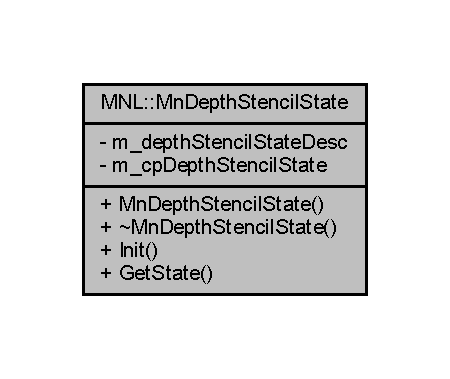
\includegraphics[width=216pt]{class_m_n_l_1_1_mn_depth_stencil_state__coll__graph}
\end{center}
\end{figure}
\subsection*{Public 멤버 함수}
\begin{DoxyCompactItemize}
\item 
\hyperlink{class_m_n_l_1_1_mn_depth_stencil_state_ac8c5a5415f93b0a54837bcfd88e36ab3}{Mn\+Depth\+Stencil\+State} ()
\item 
\hyperlink{class_m_n_l_1_1_mn_depth_stencil_state_a69ad219841e29b837080c7d35d6345b8}{$\sim$\+Mn\+Depth\+Stencil\+State} ()
\item 
H\+R\+E\+S\+U\+LT \hyperlink{class_m_n_l_1_1_mn_depth_stencil_state_a3c269bcb6437435f134cbb1e2e761b0f}{Init} (\hyperlink{namespace_m_n_l_a1eec210db8f309a4a9ac0d9658784c31}{C\+P\+D3\+D\+Device} cp\+Device, bool depth\+Enable, bool stencil\+Enable)
\item 
const \hyperlink{namespace_m_n_l_a8209b06065c025e5d6bc2e8ee5925faf}{C\+P\+D3\+D\+Depth\+Stencil\+State} \hyperlink{class_m_n_l_1_1_mn_depth_stencil_state_aceb187c0cf267621b631531cac28bd27}{Get\+State} () const
\end{DoxyCompactItemize}
\subsection*{Private 속성}
\begin{DoxyCompactItemize}
\item 
D3\+D11\+\_\+\+D\+E\+P\+T\+H\+\_\+\+S\+T\+E\+N\+C\+I\+L\+\_\+\+D\+E\+SC \hyperlink{class_m_n_l_1_1_mn_depth_stencil_state_a1d4dc90b80e4f447f6a64a8cfcd53c72}{m\+\_\+depth\+Stencil\+State\+Desc}
\item 
\hyperlink{namespace_m_n_l_a8209b06065c025e5d6bc2e8ee5925faf}{C\+P\+D3\+D\+Depth\+Stencil\+State} \hyperlink{class_m_n_l_1_1_mn_depth_stencil_state_a23bb91aaa4077752afe743a2385a04bc}{m\+\_\+cp\+Depth\+Stencil\+State}
\end{DoxyCompactItemize}


\subsection{상세한 설명}


Mn\+Depth\+Stencil\+State.\+h 파일의 7 번째 라인에서 정의되었습니다.



\subsection{생성자 \& 소멸자 문서화}
\mbox{\Hypertarget{class_m_n_l_1_1_mn_depth_stencil_state_ac8c5a5415f93b0a54837bcfd88e36ab3}\label{class_m_n_l_1_1_mn_depth_stencil_state_ac8c5a5415f93b0a54837bcfd88e36ab3}} 
\index{M\+N\+L\+::\+Mn\+Depth\+Stencil\+State@{M\+N\+L\+::\+Mn\+Depth\+Stencil\+State}!Mn\+Depth\+Stencil\+State@{Mn\+Depth\+Stencil\+State}}
\index{Mn\+Depth\+Stencil\+State@{Mn\+Depth\+Stencil\+State}!M\+N\+L\+::\+Mn\+Depth\+Stencil\+State@{M\+N\+L\+::\+Mn\+Depth\+Stencil\+State}}
\subsubsection{\texorpdfstring{Mn\+Depth\+Stencil\+State()}{MnDepthStencilState()}}
{\footnotesize\ttfamily Mn\+Depth\+Stencil\+State\+::\+Mn\+Depth\+Stencil\+State (\begin{DoxyParamCaption}{ }\end{DoxyParamCaption})}



Mn\+Depth\+Stencil\+State.\+cpp 파일의 6 번째 라인에서 정의되었습니다.

\mbox{\Hypertarget{class_m_n_l_1_1_mn_depth_stencil_state_a69ad219841e29b837080c7d35d6345b8}\label{class_m_n_l_1_1_mn_depth_stencil_state_a69ad219841e29b837080c7d35d6345b8}} 
\index{M\+N\+L\+::\+Mn\+Depth\+Stencil\+State@{M\+N\+L\+::\+Mn\+Depth\+Stencil\+State}!````~Mn\+Depth\+Stencil\+State@{$\sim$\+Mn\+Depth\+Stencil\+State}}
\index{````~Mn\+Depth\+Stencil\+State@{$\sim$\+Mn\+Depth\+Stencil\+State}!M\+N\+L\+::\+Mn\+Depth\+Stencil\+State@{M\+N\+L\+::\+Mn\+Depth\+Stencil\+State}}
\subsubsection{\texorpdfstring{$\sim$\+Mn\+Depth\+Stencil\+State()}{~MnDepthStencilState()}}
{\footnotesize\ttfamily Mn\+Depth\+Stencil\+State\+::$\sim$\+Mn\+Depth\+Stencil\+State (\begin{DoxyParamCaption}{ }\end{DoxyParamCaption})}



Mn\+Depth\+Stencil\+State.\+cpp 파일의 12 번째 라인에서 정의되었습니다.



\subsection{멤버 함수 문서화}
\mbox{\Hypertarget{class_m_n_l_1_1_mn_depth_stencil_state_aceb187c0cf267621b631531cac28bd27}\label{class_m_n_l_1_1_mn_depth_stencil_state_aceb187c0cf267621b631531cac28bd27}} 
\index{M\+N\+L\+::\+Mn\+Depth\+Stencil\+State@{M\+N\+L\+::\+Mn\+Depth\+Stencil\+State}!Get\+State@{Get\+State}}
\index{Get\+State@{Get\+State}!M\+N\+L\+::\+Mn\+Depth\+Stencil\+State@{M\+N\+L\+::\+Mn\+Depth\+Stencil\+State}}
\subsubsection{\texorpdfstring{Get\+State()}{GetState()}}
{\footnotesize\ttfamily const \hyperlink{namespace_m_n_l_a8209b06065c025e5d6bc2e8ee5925faf}{C\+P\+D3\+D\+Depth\+Stencil\+State} Mn\+Depth\+Stencil\+State\+::\+Get\+State (\begin{DoxyParamCaption}{ }\end{DoxyParamCaption}) const}



Mn\+Depth\+Stencil\+State.\+cpp 파일의 47 번째 라인에서 정의되었습니다.

\mbox{\Hypertarget{class_m_n_l_1_1_mn_depth_stencil_state_a3c269bcb6437435f134cbb1e2e761b0f}\label{class_m_n_l_1_1_mn_depth_stencil_state_a3c269bcb6437435f134cbb1e2e761b0f}} 
\index{M\+N\+L\+::\+Mn\+Depth\+Stencil\+State@{M\+N\+L\+::\+Mn\+Depth\+Stencil\+State}!Init@{Init}}
\index{Init@{Init}!M\+N\+L\+::\+Mn\+Depth\+Stencil\+State@{M\+N\+L\+::\+Mn\+Depth\+Stencil\+State}}
\subsubsection{\texorpdfstring{Init()}{Init()}}
{\footnotesize\ttfamily H\+R\+E\+S\+U\+LT Mn\+Depth\+Stencil\+State\+::\+Init (\begin{DoxyParamCaption}\item[{\hyperlink{namespace_m_n_l_a1eec210db8f309a4a9ac0d9658784c31}{C\+P\+D3\+D\+Device}}]{cp\+Device,  }\item[{bool}]{depth\+Enable,  }\item[{bool}]{stencil\+Enable }\end{DoxyParamCaption})}



Mn\+Depth\+Stencil\+State.\+cpp 파일의 16 번째 라인에서 정의되었습니다.



\subsection{멤버 데이터 문서화}
\mbox{\Hypertarget{class_m_n_l_1_1_mn_depth_stencil_state_a23bb91aaa4077752afe743a2385a04bc}\label{class_m_n_l_1_1_mn_depth_stencil_state_a23bb91aaa4077752afe743a2385a04bc}} 
\index{M\+N\+L\+::\+Mn\+Depth\+Stencil\+State@{M\+N\+L\+::\+Mn\+Depth\+Stencil\+State}!m\+\_\+cp\+Depth\+Stencil\+State@{m\+\_\+cp\+Depth\+Stencil\+State}}
\index{m\+\_\+cp\+Depth\+Stencil\+State@{m\+\_\+cp\+Depth\+Stencil\+State}!M\+N\+L\+::\+Mn\+Depth\+Stencil\+State@{M\+N\+L\+::\+Mn\+Depth\+Stencil\+State}}
\subsubsection{\texorpdfstring{m\+\_\+cp\+Depth\+Stencil\+State}{m\_cpDepthStencilState}}
{\footnotesize\ttfamily \hyperlink{namespace_m_n_l_a8209b06065c025e5d6bc2e8ee5925faf}{C\+P\+D3\+D\+Depth\+Stencil\+State} M\+N\+L\+::\+Mn\+Depth\+Stencil\+State\+::m\+\_\+cp\+Depth\+Stencil\+State\hspace{0.3cm}{\ttfamily [private]}}



Mn\+Depth\+Stencil\+State.\+h 파일의 18 번째 라인에서 정의되었습니다.

\mbox{\Hypertarget{class_m_n_l_1_1_mn_depth_stencil_state_a1d4dc90b80e4f447f6a64a8cfcd53c72}\label{class_m_n_l_1_1_mn_depth_stencil_state_a1d4dc90b80e4f447f6a64a8cfcd53c72}} 
\index{M\+N\+L\+::\+Mn\+Depth\+Stencil\+State@{M\+N\+L\+::\+Mn\+Depth\+Stencil\+State}!m\+\_\+depth\+Stencil\+State\+Desc@{m\+\_\+depth\+Stencil\+State\+Desc}}
\index{m\+\_\+depth\+Stencil\+State\+Desc@{m\+\_\+depth\+Stencil\+State\+Desc}!M\+N\+L\+::\+Mn\+Depth\+Stencil\+State@{M\+N\+L\+::\+Mn\+Depth\+Stencil\+State}}
\subsubsection{\texorpdfstring{m\+\_\+depth\+Stencil\+State\+Desc}{m\_depthStencilStateDesc}}
{\footnotesize\ttfamily D3\+D11\+\_\+\+D\+E\+P\+T\+H\+\_\+\+S\+T\+E\+N\+C\+I\+L\+\_\+\+D\+E\+SC M\+N\+L\+::\+Mn\+Depth\+Stencil\+State\+::m\+\_\+depth\+Stencil\+State\+Desc\hspace{0.3cm}{\ttfamily [private]}}



Mn\+Depth\+Stencil\+State.\+h 파일의 17 번째 라인에서 정의되었습니다.



이 클래스에 대한 문서화 페이지는 다음의 파일들로부터 생성되었습니다.\+:\begin{DoxyCompactItemize}
\item 
Core/\hyperlink{_mn_depth_stencil_state_8h}{Mn\+Depth\+Stencil\+State.\+h}\item 
Core/\hyperlink{_mn_depth_stencil_state_8cpp}{Mn\+Depth\+Stencil\+State.\+cpp}\end{DoxyCompactItemize}

\hypertarget{class_m_n_l_1_1_mn_display_device}{}\section{M\+NL\+:\+:Mn\+Display\+Device 클래스 참조}
\label{class_m_n_l_1_1_mn_display_device}\index{M\+N\+L\+::\+Mn\+Display\+Device@{M\+N\+L\+::\+Mn\+Display\+Device}}


디스플레이 장치의 디스플레이 모드 정보를 얻어와 저장한다.  




{\ttfamily \#include $<$Mn\+Display\+Device.\+h$>$}



M\+NL\+:\+:Mn\+Display\+Device에 대한 협력 다이어그램\+:\nopagebreak
\begin{figure}[H]
\begin{center}
\leavevmode
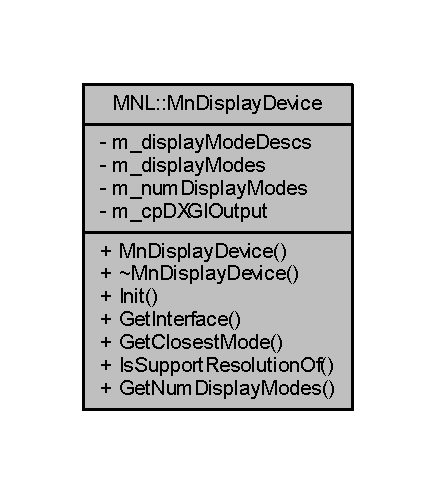
\includegraphics[width=209pt]{class_m_n_l_1_1_mn_display_device__coll__graph}
\end{center}
\end{figure}
\subsection*{Public 멤버 함수}
\begin{DoxyCompactItemize}
\item 
\hyperlink{class_m_n_l_1_1_mn_display_device_af7f8cbdfc1a219e619930df164ef1b1b}{Mn\+Display\+Device} ()
\item 
\hyperlink{class_m_n_l_1_1_mn_display_device_a482d7838429f83ed1676d6a784dade88}{$\sim$\+Mn\+Display\+Device} ()
\item 
H\+R\+E\+S\+U\+LT \hyperlink{class_m_n_l_1_1_mn_display_device_a59739c090a5a2a6b704d93622a22f6ef}{Init} (\hyperlink{namespace_m_n_l_ac03add2215d9e5f2938af7887c5b09de}{C\+P\+D\+X\+G\+I\+Output} cp\+Output)
\begin{DoxyCompactList}\small\item\em D\+X\+G\+I\+Output 인터페이스를 통해 모든 디스플레이 모드들을 얻어와 초기화 한다. \end{DoxyCompactList}\item 
const \hyperlink{namespace_m_n_l_ac03add2215d9e5f2938af7887c5b09de}{C\+P\+D\+X\+G\+I\+Output} \hyperlink{class_m_n_l_1_1_mn_display_device_a38f042976af5b2ff72ba37c545fa9895}{Get\+Interface} () const
\begin{DoxyCompactList}\small\item\em D\+X\+G\+I\+Output 인터페이스를 반환한다. \end{DoxyCompactList}\item 
\hyperlink{struct_m_n_l_1_1_mn_display_mode}{Mn\+Display\+Mode} \hyperlink{class_m_n_l_1_1_mn_display_device_a8190e43b743203ccd485061df6e37565}{Get\+Closest\+Mode} (U\+I\+NT width, U\+I\+NT height, U\+I\+NT numerator, U\+I\+NT denominator) const
\begin{DoxyCompactList}\small\item\em 지원되는 디스플레이 모드 중 가장 흡사한 디스플레이 모드를 찾아 반환한다. \end{DoxyCompactList}\item 
bool \hyperlink{class_m_n_l_1_1_mn_display_device_a4180fb0187da5e3751bca74fb46880a3}{Is\+Support\+Resolution\+Of} (U\+I\+NT width, U\+I\+NT height) const
\begin{DoxyCompactList}\small\item\em 해당 해상도를 지원하는지 여부를 반환한다. \end{DoxyCompactList}\item 
U\+I\+NT \hyperlink{class_m_n_l_1_1_mn_display_device_a11b7ecaf93de4b94fd563a4e0cbebd80}{Get\+Num\+Display\+Modes} () const
\end{DoxyCompactItemize}
\subsection*{Private 속성}
\begin{DoxyCompactItemize}
\item 
std\+::vector$<$ D\+X\+G\+I\+\_\+\+M\+O\+D\+E\+\_\+\+D\+E\+SC $>$ \hyperlink{class_m_n_l_1_1_mn_display_device_a496e5f393dc60c67504da2a35a863728}{m\+\_\+display\+Mode\+Descs}
\begin{DoxyCompactList}\small\item\em 디스플레이 명세가 저장된 컨테이너 \end{DoxyCompactList}\item 
std\+::vector$<$ \hyperlink{struct_m_n_l_1_1_mn_display_mode}{Mn\+Display\+Mode} $>$ \hyperlink{class_m_n_l_1_1_mn_display_device_a78c903529f9107d3f5b0fa14d2e4fd34}{m\+\_\+display\+Modes}
\begin{DoxyCompactList}\small\item\em 디스플레이 모드가 저장된 컨테이너 \end{DoxyCompactList}\item 
U\+I\+NT \hyperlink{class_m_n_l_1_1_mn_display_device_abdc40d78874813d1b4ce802a65247464}{m\+\_\+num\+Display\+Modes}
\begin{DoxyCompactList}\small\item\em 디스플레이 모드 개수 \end{DoxyCompactList}\item 
\hyperlink{namespace_m_n_l_ac03add2215d9e5f2938af7887c5b09de}{C\+P\+D\+X\+G\+I\+Output} \hyperlink{class_m_n_l_1_1_mn_display_device_a718cf72ca95ace1f6dcc4d31daea6be9}{m\+\_\+cp\+D\+X\+G\+I\+Output}
\begin{DoxyCompactList}\small\item\em D\+X\+G\+I\+Output 인터페이스 \end{DoxyCompactList}\end{DoxyCompactItemize}


\subsection{상세한 설명}
디스플레이 장치의 디스플레이 모드 정보를 얻어와 저장한다. 

\begin{DoxyAuthor}{작성자}
Akssus 
\end{DoxyAuthor}
\hypertarget{class_m_n_l_1_1_mn_video_adapter_개요}{}\subsection{개요}\label{class_m_n_l_1_1_mn_video_adapter_개요}
하나의 Display\+Device는 하나의 디스플레이 장치(모니터)의 정보를 담고 있다.~\newline
지원하는 모든 해상도의 종류, 주사율 등의 정보를 제공하며 특정 해상도가 지원되는지 여부를 알 수 있다.~\newline
추가로 주어진 조건과 가장 가까운 지원되는 Display Mode를 찾아내는 Get\+Closest\+Mode 메소드를 제공한다.~\newline
이 메소드가 필요한 이유는 이런 메소드가 없으면 사용자 혹은 개발자가 모니터가 지원하는 완벽하게 정확한 해상도와 주사율 값을 알아야 하기 때문에 불편하기 때문이다.~\newline


Mn\+Display\+Device.\+h 파일의 30 번째 라인에서 정의되었습니다.



\subsection{생성자 \& 소멸자 문서화}
\mbox{\Hypertarget{class_m_n_l_1_1_mn_display_device_af7f8cbdfc1a219e619930df164ef1b1b}\label{class_m_n_l_1_1_mn_display_device_af7f8cbdfc1a219e619930df164ef1b1b}} 
\index{M\+N\+L\+::\+Mn\+Display\+Device@{M\+N\+L\+::\+Mn\+Display\+Device}!Mn\+Display\+Device@{Mn\+Display\+Device}}
\index{Mn\+Display\+Device@{Mn\+Display\+Device}!M\+N\+L\+::\+Mn\+Display\+Device@{M\+N\+L\+::\+Mn\+Display\+Device}}
\subsubsection{\texorpdfstring{Mn\+Display\+Device()}{MnDisplayDevice()}}
{\footnotesize\ttfamily Mn\+Display\+Device\+::\+Mn\+Display\+Device (\begin{DoxyParamCaption}{ }\end{DoxyParamCaption})}



Mn\+Display\+Device.\+cpp 파일의 9 번째 라인에서 정의되었습니다.

\mbox{\Hypertarget{class_m_n_l_1_1_mn_display_device_a482d7838429f83ed1676d6a784dade88}\label{class_m_n_l_1_1_mn_display_device_a482d7838429f83ed1676d6a784dade88}} 
\index{M\+N\+L\+::\+Mn\+Display\+Device@{M\+N\+L\+::\+Mn\+Display\+Device}!````~Mn\+Display\+Device@{$\sim$\+Mn\+Display\+Device}}
\index{````~Mn\+Display\+Device@{$\sim$\+Mn\+Display\+Device}!M\+N\+L\+::\+Mn\+Display\+Device@{M\+N\+L\+::\+Mn\+Display\+Device}}
\subsubsection{\texorpdfstring{$\sim$\+Mn\+Display\+Device()}{~MnDisplayDevice()}}
{\footnotesize\ttfamily Mn\+Display\+Device\+::$\sim$\+Mn\+Display\+Device (\begin{DoxyParamCaption}{ }\end{DoxyParamCaption})}



Mn\+Display\+Device.\+cpp 파일의 14 번째 라인에서 정의되었습니다.



\subsection{멤버 함수 문서화}
\mbox{\Hypertarget{class_m_n_l_1_1_mn_display_device_a8190e43b743203ccd485061df6e37565}\label{class_m_n_l_1_1_mn_display_device_a8190e43b743203ccd485061df6e37565}} 
\index{M\+N\+L\+::\+Mn\+Display\+Device@{M\+N\+L\+::\+Mn\+Display\+Device}!Get\+Closest\+Mode@{Get\+Closest\+Mode}}
\index{Get\+Closest\+Mode@{Get\+Closest\+Mode}!M\+N\+L\+::\+Mn\+Display\+Device@{M\+N\+L\+::\+Mn\+Display\+Device}}
\subsubsection{\texorpdfstring{Get\+Closest\+Mode()}{GetClosestMode()}}
{\footnotesize\ttfamily \hyperlink{struct_m_n_l_1_1_mn_display_mode}{Mn\+Display\+Mode} Mn\+Display\+Device\+::\+Get\+Closest\+Mode (\begin{DoxyParamCaption}\item[{U\+I\+NT}]{width,  }\item[{U\+I\+NT}]{height,  }\item[{U\+I\+NT}]{numerator,  }\item[{U\+I\+NT}]{denominator }\end{DoxyParamCaption}) const}



지원되는 디스플레이 모드 중 가장 흡사한 디스플레이 모드를 찾아 반환한다. 


\begin{DoxyParams}{매개변수}
{\em width} & 해상도 넓이 \\
\hline
{\em height} & 해상도 높이 \\
\hline
{\em numerator} & 주사율의 분자 \\
\hline
{\em denominator} & 주사율 분모 \\
\hline
\end{DoxyParams}


Mn\+Display\+Device.\+cpp 파일의 52 번째 라인에서 정의되었습니다.

\mbox{\Hypertarget{class_m_n_l_1_1_mn_display_device_a38f042976af5b2ff72ba37c545fa9895}\label{class_m_n_l_1_1_mn_display_device_a38f042976af5b2ff72ba37c545fa9895}} 
\index{M\+N\+L\+::\+Mn\+Display\+Device@{M\+N\+L\+::\+Mn\+Display\+Device}!Get\+Interface@{Get\+Interface}}
\index{Get\+Interface@{Get\+Interface}!M\+N\+L\+::\+Mn\+Display\+Device@{M\+N\+L\+::\+Mn\+Display\+Device}}
\subsubsection{\texorpdfstring{Get\+Interface()}{GetInterface()}}
{\footnotesize\ttfamily const \hyperlink{namespace_m_n_l_ac03add2215d9e5f2938af7887c5b09de}{C\+P\+D\+X\+G\+I\+Output} Mn\+Display\+Device\+::\+Get\+Interface (\begin{DoxyParamCaption}{ }\end{DoxyParamCaption}) const}



D\+X\+G\+I\+Output 인터페이스를 반환한다. 



Mn\+Display\+Device.\+cpp 파일의 48 번째 라인에서 정의되었습니다.

\mbox{\Hypertarget{class_m_n_l_1_1_mn_display_device_a11b7ecaf93de4b94fd563a4e0cbebd80}\label{class_m_n_l_1_1_mn_display_device_a11b7ecaf93de4b94fd563a4e0cbebd80}} 
\index{M\+N\+L\+::\+Mn\+Display\+Device@{M\+N\+L\+::\+Mn\+Display\+Device}!Get\+Num\+Display\+Modes@{Get\+Num\+Display\+Modes}}
\index{Get\+Num\+Display\+Modes@{Get\+Num\+Display\+Modes}!M\+N\+L\+::\+Mn\+Display\+Device@{M\+N\+L\+::\+Mn\+Display\+Device}}
\subsubsection{\texorpdfstring{Get\+Num\+Display\+Modes()}{GetNumDisplayModes()}}
{\footnotesize\ttfamily U\+I\+NT Mn\+Display\+Device\+::\+Get\+Num\+Display\+Modes (\begin{DoxyParamCaption}{ }\end{DoxyParamCaption}) const}

현재 디스플레이 장치의 디스플레이 모드 개수를 반환한다. 

Mn\+Display\+Device.\+cpp 파일의 108 번째 라인에서 정의되었습니다.

\mbox{\Hypertarget{class_m_n_l_1_1_mn_display_device_a59739c090a5a2a6b704d93622a22f6ef}\label{class_m_n_l_1_1_mn_display_device_a59739c090a5a2a6b704d93622a22f6ef}} 
\index{M\+N\+L\+::\+Mn\+Display\+Device@{M\+N\+L\+::\+Mn\+Display\+Device}!Init@{Init}}
\index{Init@{Init}!M\+N\+L\+::\+Mn\+Display\+Device@{M\+N\+L\+::\+Mn\+Display\+Device}}
\subsubsection{\texorpdfstring{Init()}{Init()}}
{\footnotesize\ttfamily H\+R\+E\+S\+U\+LT Mn\+Display\+Device\+::\+Init (\begin{DoxyParamCaption}\item[{\hyperlink{namespace_m_n_l_ac03add2215d9e5f2938af7887c5b09de}{C\+P\+D\+X\+G\+I\+Output}}]{cp\+Output }\end{DoxyParamCaption})}



D\+X\+G\+I\+Output 인터페이스를 통해 모든 디스플레이 모드들을 얻어와 초기화 한다. 

\begin{DoxyReturn}{반환값}
초기화 성공 여부. 
\end{DoxyReturn}


Mn\+Display\+Device.\+cpp 파일의 18 번째 라인에서 정의되었습니다.

\mbox{\Hypertarget{class_m_n_l_1_1_mn_display_device_a4180fb0187da5e3751bca74fb46880a3}\label{class_m_n_l_1_1_mn_display_device_a4180fb0187da5e3751bca74fb46880a3}} 
\index{M\+N\+L\+::\+Mn\+Display\+Device@{M\+N\+L\+::\+Mn\+Display\+Device}!Is\+Support\+Resolution\+Of@{Is\+Support\+Resolution\+Of}}
\index{Is\+Support\+Resolution\+Of@{Is\+Support\+Resolution\+Of}!M\+N\+L\+::\+Mn\+Display\+Device@{M\+N\+L\+::\+Mn\+Display\+Device}}
\subsubsection{\texorpdfstring{Is\+Support\+Resolution\+Of()}{IsSupportResolutionOf()}}
{\footnotesize\ttfamily bool Mn\+Display\+Device\+::\+Is\+Support\+Resolution\+Of (\begin{DoxyParamCaption}\item[{U\+I\+NT}]{width,  }\item[{U\+I\+NT}]{height }\end{DoxyParamCaption}) const}



해당 해상도를 지원하는지 여부를 반환한다. 

\begin{DoxyReturn}{반환값}
지원할 경우 true 반환. 
\end{DoxyReturn}


Mn\+Display\+Device.\+cpp 파일의 94 번째 라인에서 정의되었습니다.



\subsection{멤버 데이터 문서화}
\mbox{\Hypertarget{class_m_n_l_1_1_mn_display_device_a718cf72ca95ace1f6dcc4d31daea6be9}\label{class_m_n_l_1_1_mn_display_device_a718cf72ca95ace1f6dcc4d31daea6be9}} 
\index{M\+N\+L\+::\+Mn\+Display\+Device@{M\+N\+L\+::\+Mn\+Display\+Device}!m\+\_\+cp\+D\+X\+G\+I\+Output@{m\+\_\+cp\+D\+X\+G\+I\+Output}}
\index{m\+\_\+cp\+D\+X\+G\+I\+Output@{m\+\_\+cp\+D\+X\+G\+I\+Output}!M\+N\+L\+::\+Mn\+Display\+Device@{M\+N\+L\+::\+Mn\+Display\+Device}}
\subsubsection{\texorpdfstring{m\+\_\+cp\+D\+X\+G\+I\+Output}{m\_cpDXGIOutput}}
{\footnotesize\ttfamily \hyperlink{namespace_m_n_l_ac03add2215d9e5f2938af7887c5b09de}{C\+P\+D\+X\+G\+I\+Output} M\+N\+L\+::\+Mn\+Display\+Device\+::m\+\_\+cp\+D\+X\+G\+I\+Output\hspace{0.3cm}{\ttfamily [private]}}



D\+X\+G\+I\+Output 인터페이스 



Mn\+Display\+Device.\+h 파일의 73 번째 라인에서 정의되었습니다.

\mbox{\Hypertarget{class_m_n_l_1_1_mn_display_device_a496e5f393dc60c67504da2a35a863728}\label{class_m_n_l_1_1_mn_display_device_a496e5f393dc60c67504da2a35a863728}} 
\index{M\+N\+L\+::\+Mn\+Display\+Device@{M\+N\+L\+::\+Mn\+Display\+Device}!m\+\_\+display\+Mode\+Descs@{m\+\_\+display\+Mode\+Descs}}
\index{m\+\_\+display\+Mode\+Descs@{m\+\_\+display\+Mode\+Descs}!M\+N\+L\+::\+Mn\+Display\+Device@{M\+N\+L\+::\+Mn\+Display\+Device}}
\subsubsection{\texorpdfstring{m\+\_\+display\+Mode\+Descs}{m\_displayModeDescs}}
{\footnotesize\ttfamily std\+::vector$<$D\+X\+G\+I\+\_\+\+M\+O\+D\+E\+\_\+\+D\+E\+SC$>$ M\+N\+L\+::\+Mn\+Display\+Device\+::m\+\_\+display\+Mode\+Descs\hspace{0.3cm}{\ttfamily [private]}}



디스플레이 명세가 저장된 컨테이너 



Mn\+Display\+Device.\+h 파일의 70 번째 라인에서 정의되었습니다.

\mbox{\Hypertarget{class_m_n_l_1_1_mn_display_device_a78c903529f9107d3f5b0fa14d2e4fd34}\label{class_m_n_l_1_1_mn_display_device_a78c903529f9107d3f5b0fa14d2e4fd34}} 
\index{M\+N\+L\+::\+Mn\+Display\+Device@{M\+N\+L\+::\+Mn\+Display\+Device}!m\+\_\+display\+Modes@{m\+\_\+display\+Modes}}
\index{m\+\_\+display\+Modes@{m\+\_\+display\+Modes}!M\+N\+L\+::\+Mn\+Display\+Device@{M\+N\+L\+::\+Mn\+Display\+Device}}
\subsubsection{\texorpdfstring{m\+\_\+display\+Modes}{m\_displayModes}}
{\footnotesize\ttfamily std\+::vector$<$\hyperlink{struct_m_n_l_1_1_mn_display_mode}{Mn\+Display\+Mode}$>$ M\+N\+L\+::\+Mn\+Display\+Device\+::m\+\_\+display\+Modes\hspace{0.3cm}{\ttfamily [private]}}



디스플레이 모드가 저장된 컨테이너 



Mn\+Display\+Device.\+h 파일의 71 번째 라인에서 정의되었습니다.

\mbox{\Hypertarget{class_m_n_l_1_1_mn_display_device_abdc40d78874813d1b4ce802a65247464}\label{class_m_n_l_1_1_mn_display_device_abdc40d78874813d1b4ce802a65247464}} 
\index{M\+N\+L\+::\+Mn\+Display\+Device@{M\+N\+L\+::\+Mn\+Display\+Device}!m\+\_\+num\+Display\+Modes@{m\+\_\+num\+Display\+Modes}}
\index{m\+\_\+num\+Display\+Modes@{m\+\_\+num\+Display\+Modes}!M\+N\+L\+::\+Mn\+Display\+Device@{M\+N\+L\+::\+Mn\+Display\+Device}}
\subsubsection{\texorpdfstring{m\+\_\+num\+Display\+Modes}{m\_numDisplayModes}}
{\footnotesize\ttfamily U\+I\+NT M\+N\+L\+::\+Mn\+Display\+Device\+::m\+\_\+num\+Display\+Modes\hspace{0.3cm}{\ttfamily [private]}}



디스플레이 모드 개수 



Mn\+Display\+Device.\+h 파일의 72 번째 라인에서 정의되었습니다.



이 클래스에 대한 문서화 페이지는 다음의 파일들로부터 생성되었습니다.\+:\begin{DoxyCompactItemize}
\item 
Core/\hyperlink{_mn_display_device_8h}{Mn\+Display\+Device.\+h}\item 
Core/\hyperlink{_mn_display_device_8cpp}{Mn\+Display\+Device.\+cpp}\end{DoxyCompactItemize}

\hypertarget{struct_m_n_l_1_1_mn_display_mode}{}\section{M\+NL\+:\+:Mn\+Display\+Mode 구조체 참조}
\label{struct_m_n_l_1_1_mn_display_mode}\index{M\+N\+L\+::\+Mn\+Display\+Mode@{M\+N\+L\+::\+Mn\+Display\+Mode}}


디스플레이 모드 정보를 담고있다.  




{\ttfamily \#include $<$Mn\+Display\+Device.\+h$>$}



M\+NL\+:\+:Mn\+Display\+Mode에 대한 협력 다이어그램\+:\nopagebreak
\begin{figure}[H]
\begin{center}
\leavevmode
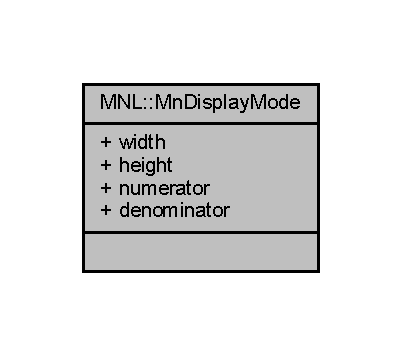
\includegraphics[width=193pt]{struct_m_n_l_1_1_mn_display_mode__coll__graph}
\end{center}
\end{figure}
\subsection*{Public 속성}
\begin{DoxyCompactItemize}
\item 
U\+I\+NT \hyperlink{struct_m_n_l_1_1_mn_display_mode_a483b98018ae07b10bfbf3c42d234550e}{width}
\item 
U\+I\+NT \hyperlink{struct_m_n_l_1_1_mn_display_mode_acc4e550e9b762236a0eae7298128bf06}{height}
\item 
U\+I\+NT \hyperlink{struct_m_n_l_1_1_mn_display_mode_a4049edd40bf11c67c6d85709ec4450ee}{numerator}
\item 
U\+I\+NT \hyperlink{struct_m_n_l_1_1_mn_display_mode_af891810b084193ba0f48557a747d04ab}{denominator}
\end{DoxyCompactItemize}


\subsection{상세한 설명}
디스플레이 모드 정보를 담고있다. 

Mn\+Display\+Device.\+h 파일의 25 번째 라인에서 정의되었습니다.



\subsection{멤버 데이터 문서화}
\mbox{\Hypertarget{struct_m_n_l_1_1_mn_display_mode_af891810b084193ba0f48557a747d04ab}\label{struct_m_n_l_1_1_mn_display_mode_af891810b084193ba0f48557a747d04ab}} 
\index{M\+N\+L\+::\+Mn\+Display\+Mode@{M\+N\+L\+::\+Mn\+Display\+Mode}!denominator@{denominator}}
\index{denominator@{denominator}!M\+N\+L\+::\+Mn\+Display\+Mode@{M\+N\+L\+::\+Mn\+Display\+Mode}}
\subsubsection{\texorpdfstring{denominator}{denominator}}
{\footnotesize\ttfamily U\+I\+NT M\+N\+L\+::\+Mn\+Display\+Mode\+::denominator}



Mn\+Display\+Device.\+h 파일의 28 번째 라인에서 정의되었습니다.

\mbox{\Hypertarget{struct_m_n_l_1_1_mn_display_mode_acc4e550e9b762236a0eae7298128bf06}\label{struct_m_n_l_1_1_mn_display_mode_acc4e550e9b762236a0eae7298128bf06}} 
\index{M\+N\+L\+::\+Mn\+Display\+Mode@{M\+N\+L\+::\+Mn\+Display\+Mode}!height@{height}}
\index{height@{height}!M\+N\+L\+::\+Mn\+Display\+Mode@{M\+N\+L\+::\+Mn\+Display\+Mode}}
\subsubsection{\texorpdfstring{height}{height}}
{\footnotesize\ttfamily U\+I\+NT M\+N\+L\+::\+Mn\+Display\+Mode\+::height}



Mn\+Display\+Device.\+h 파일의 27 번째 라인에서 정의되었습니다.

\mbox{\Hypertarget{struct_m_n_l_1_1_mn_display_mode_a4049edd40bf11c67c6d85709ec4450ee}\label{struct_m_n_l_1_1_mn_display_mode_a4049edd40bf11c67c6d85709ec4450ee}} 
\index{M\+N\+L\+::\+Mn\+Display\+Mode@{M\+N\+L\+::\+Mn\+Display\+Mode}!numerator@{numerator}}
\index{numerator@{numerator}!M\+N\+L\+::\+Mn\+Display\+Mode@{M\+N\+L\+::\+Mn\+Display\+Mode}}
\subsubsection{\texorpdfstring{numerator}{numerator}}
{\footnotesize\ttfamily U\+I\+NT M\+N\+L\+::\+Mn\+Display\+Mode\+::numerator}



Mn\+Display\+Device.\+h 파일의 28 번째 라인에서 정의되었습니다.

\mbox{\Hypertarget{struct_m_n_l_1_1_mn_display_mode_a483b98018ae07b10bfbf3c42d234550e}\label{struct_m_n_l_1_1_mn_display_mode_a483b98018ae07b10bfbf3c42d234550e}} 
\index{M\+N\+L\+::\+Mn\+Display\+Mode@{M\+N\+L\+::\+Mn\+Display\+Mode}!width@{width}}
\index{width@{width}!M\+N\+L\+::\+Mn\+Display\+Mode@{M\+N\+L\+::\+Mn\+Display\+Mode}}
\subsubsection{\texorpdfstring{width}{width}}
{\footnotesize\ttfamily U\+I\+NT M\+N\+L\+::\+Mn\+Display\+Mode\+::width}



Mn\+Display\+Device.\+h 파일의 27 번째 라인에서 정의되었습니다.



이 구조체에 대한 문서화 페이지는 다음의 파일로부터 생성되었습니다.\+:\begin{DoxyCompactItemize}
\item 
Core/\hyperlink{_mn_display_device_8h}{Mn\+Display\+Device.\+h}\end{DoxyCompactItemize}

\hypertarget{class_m_n_l_1_1_mn_gpu_buffer}{}\section{M\+NL\+:\+:Mn\+Gpu\+Buffer 클래스 참조}
\label{class_m_n_l_1_1_mn_gpu_buffer}\index{M\+N\+L\+::\+Mn\+Gpu\+Buffer@{M\+N\+L\+::\+Mn\+Gpu\+Buffer}}


{\ttfamily \#include $<$Mn\+Gpu\+Buffer.\+h$>$}



M\+NL\+:\+:Mn\+Gpu\+Buffer에 대한 협력 다이어그램\+:\nopagebreak
\begin{figure}[H]
\begin{center}
\leavevmode
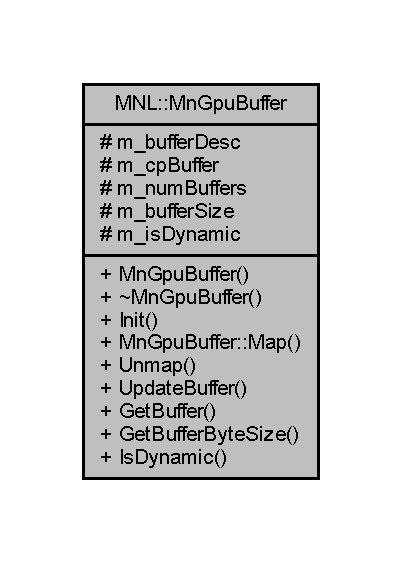
\includegraphics[width=193pt]{class_m_n_l_1_1_mn_gpu_buffer__coll__graph}
\end{center}
\end{figure}
\subsection*{Public 멤버 함수}
\begin{DoxyCompactItemize}
\item 
\hyperlink{class_m_n_l_1_1_mn_gpu_buffer_a7384edf2315dcacd76e090bd80cf3c72}{Mn\+Gpu\+Buffer} ()
\item 
\hyperlink{class_m_n_l_1_1_mn_gpu_buffer_a6628bd8e65df697f2fd95cdb6e841a04}{$\sim$\+Mn\+Gpu\+Buffer} ()
\item 
H\+R\+E\+S\+U\+LT \hyperlink{class_m_n_l_1_1_mn_gpu_buffer_a00bd28801336391d28e6d91e99a8bef3}{Init} (const \hyperlink{namespace_m_n_l_a1eec210db8f309a4a9ac0d9658784c31}{C\+P\+D3\+D\+Device} \&cp\+Device, const D3\+D11\+\_\+\+B\+U\+F\+F\+E\+R\+\_\+\+D\+E\+SC \&buffer\+Desc, const D3\+D11\+\_\+\+S\+U\+B\+R\+E\+S\+O\+U\+R\+C\+E\+\_\+\+D\+A\+TA $\ast$initial\+Data)
\item 
D3\+D11\+\_\+\+M\+A\+P\+P\+E\+D\+\_\+\+S\+U\+B\+R\+E\+S\+O\+U\+R\+CE \hyperlink{class_m_n_l_1_1_mn_gpu_buffer_aa28d7626be0829bb89db594cf253c62d}{Mn\+Gpu\+Buffer\+::\+Map} (const \hyperlink{namespace_m_n_l_aab3aabb6c9360e44ddc8b0bb563c2107}{C\+P\+D3\+D\+Device\+Context} \&cp\+Device\+Context, U\+I\+NT subresource\+Index)
\item 
void \hyperlink{class_m_n_l_1_1_mn_gpu_buffer_a152eb5876d380e888a065328da057330}{Unmap} (const \hyperlink{namespace_m_n_l_aab3aabb6c9360e44ddc8b0bb563c2107}{C\+P\+D3\+D\+Device\+Context} \&cp\+Device\+Context, U\+I\+NT subresource\+Index)
\item 
void \hyperlink{class_m_n_l_1_1_mn_gpu_buffer_a77c025ff683cce5025b58e87d28d7549}{Update\+Buffer} (\hyperlink{namespace_m_n_l_aab3aabb6c9360e44ddc8b0bb563c2107}{C\+P\+D3\+D\+Device\+Context} cp\+Device\+Context, const D3\+D11\+\_\+\+S\+U\+B\+R\+E\+S\+O\+U\+R\+C\+E\+\_\+\+D\+A\+TA \&data)
\item 
const \hyperlink{namespace_m_n_l_aab9c90a8c27ac6410a9cc7cd89efeef1}{C\+P\+D3\+D\+Buffer} \hyperlink{class_m_n_l_1_1_mn_gpu_buffer_ae929d387721832436c24e3faf6cd375d}{Get\+Buffer} () const
\item 
U\+I\+NT \hyperlink{class_m_n_l_1_1_mn_gpu_buffer_aa6a6a785b1df73b80d33b8f3d828c618}{Get\+Buffer\+Byte\+Size} () const
\item 
bool \hyperlink{class_m_n_l_1_1_mn_gpu_buffer_a617ce607255f345962df39eec00e9593}{Is\+Dynamic} () const
\end{DoxyCompactItemize}
\subsection*{Protected 속성}
\begin{DoxyCompactItemize}
\item 
D3\+D11\+\_\+\+B\+U\+F\+F\+E\+R\+\_\+\+D\+E\+SC \hyperlink{class_m_n_l_1_1_mn_gpu_buffer_ac37d75136ddee08ebf61d2d188dd4b01}{m\+\_\+buffer\+Desc}
\item 
\hyperlink{namespace_m_n_l_aab9c90a8c27ac6410a9cc7cd89efeef1}{C\+P\+D3\+D\+Buffer} \hyperlink{class_m_n_l_1_1_mn_gpu_buffer_ac5394da182d4d9955e743b040103fba6}{m\+\_\+cp\+Buffer}
\item 
U\+I\+NT \hyperlink{class_m_n_l_1_1_mn_gpu_buffer_a440a564ce0bf811c835516627079d1a5}{m\+\_\+num\+Buffers}
\item 
U\+I\+NT \hyperlink{class_m_n_l_1_1_mn_gpu_buffer_a275688eb205f74155a813a1ba65e149f}{m\+\_\+buffer\+Size}
\item 
bool \hyperlink{class_m_n_l_1_1_mn_gpu_buffer_af93d67fac012bafe36e2a052096f63ce}{m\+\_\+is\+Dynamic}
\end{DoxyCompactItemize}


\subsection{상세한 설명}


Mn\+Gpu\+Buffer.\+h 파일의 10 번째 라인에서 정의되었습니다.



\subsection{생성자 \& 소멸자 문서화}
\mbox{\Hypertarget{class_m_n_l_1_1_mn_gpu_buffer_a7384edf2315dcacd76e090bd80cf3c72}\label{class_m_n_l_1_1_mn_gpu_buffer_a7384edf2315dcacd76e090bd80cf3c72}} 
\index{M\+N\+L\+::\+Mn\+Gpu\+Buffer@{M\+N\+L\+::\+Mn\+Gpu\+Buffer}!Mn\+Gpu\+Buffer@{Mn\+Gpu\+Buffer}}
\index{Mn\+Gpu\+Buffer@{Mn\+Gpu\+Buffer}!M\+N\+L\+::\+Mn\+Gpu\+Buffer@{M\+N\+L\+::\+Mn\+Gpu\+Buffer}}
\subsubsection{\texorpdfstring{Mn\+Gpu\+Buffer()}{MnGpuBuffer()}}
{\footnotesize\ttfamily Mn\+Gpu\+Buffer\+::\+Mn\+Gpu\+Buffer (\begin{DoxyParamCaption}{ }\end{DoxyParamCaption})}



Mn\+Gpu\+Buffer.\+cpp 파일의 6 번째 라인에서 정의되었습니다.

\mbox{\Hypertarget{class_m_n_l_1_1_mn_gpu_buffer_a6628bd8e65df697f2fd95cdb6e841a04}\label{class_m_n_l_1_1_mn_gpu_buffer_a6628bd8e65df697f2fd95cdb6e841a04}} 
\index{M\+N\+L\+::\+Mn\+Gpu\+Buffer@{M\+N\+L\+::\+Mn\+Gpu\+Buffer}!````~Mn\+Gpu\+Buffer@{$\sim$\+Mn\+Gpu\+Buffer}}
\index{````~Mn\+Gpu\+Buffer@{$\sim$\+Mn\+Gpu\+Buffer}!M\+N\+L\+::\+Mn\+Gpu\+Buffer@{M\+N\+L\+::\+Mn\+Gpu\+Buffer}}
\subsubsection{\texorpdfstring{$\sim$\+Mn\+Gpu\+Buffer()}{~MnGpuBuffer()}}
{\footnotesize\ttfamily Mn\+Gpu\+Buffer\+::$\sim$\+Mn\+Gpu\+Buffer (\begin{DoxyParamCaption}{ }\end{DoxyParamCaption})}



Mn\+Gpu\+Buffer.\+cpp 파일의 12 번째 라인에서 정의되었습니다.



\subsection{멤버 함수 문서화}
\mbox{\Hypertarget{class_m_n_l_1_1_mn_gpu_buffer_ae929d387721832436c24e3faf6cd375d}\label{class_m_n_l_1_1_mn_gpu_buffer_ae929d387721832436c24e3faf6cd375d}} 
\index{M\+N\+L\+::\+Mn\+Gpu\+Buffer@{M\+N\+L\+::\+Mn\+Gpu\+Buffer}!Get\+Buffer@{Get\+Buffer}}
\index{Get\+Buffer@{Get\+Buffer}!M\+N\+L\+::\+Mn\+Gpu\+Buffer@{M\+N\+L\+::\+Mn\+Gpu\+Buffer}}
\subsubsection{\texorpdfstring{Get\+Buffer()}{GetBuffer()}}
{\footnotesize\ttfamily const \hyperlink{namespace_m_n_l_aab9c90a8c27ac6410a9cc7cd89efeef1}{C\+P\+D3\+D\+Buffer} Mn\+Gpu\+Buffer\+::\+Get\+Buffer (\begin{DoxyParamCaption}{ }\end{DoxyParamCaption}) const}



Mn\+Gpu\+Buffer.\+cpp 파일의 53 번째 라인에서 정의되었습니다.

\mbox{\Hypertarget{class_m_n_l_1_1_mn_gpu_buffer_aa6a6a785b1df73b80d33b8f3d828c618}\label{class_m_n_l_1_1_mn_gpu_buffer_aa6a6a785b1df73b80d33b8f3d828c618}} 
\index{M\+N\+L\+::\+Mn\+Gpu\+Buffer@{M\+N\+L\+::\+Mn\+Gpu\+Buffer}!Get\+Buffer\+Byte\+Size@{Get\+Buffer\+Byte\+Size}}
\index{Get\+Buffer\+Byte\+Size@{Get\+Buffer\+Byte\+Size}!M\+N\+L\+::\+Mn\+Gpu\+Buffer@{M\+N\+L\+::\+Mn\+Gpu\+Buffer}}
\subsubsection{\texorpdfstring{Get\+Buffer\+Byte\+Size()}{GetBufferByteSize()}}
{\footnotesize\ttfamily U\+I\+NT Mn\+Gpu\+Buffer\+::\+Get\+Buffer\+Byte\+Size (\begin{DoxyParamCaption}{ }\end{DoxyParamCaption}) const}



Mn\+Gpu\+Buffer.\+cpp 파일의 48 번째 라인에서 정의되었습니다.

\mbox{\Hypertarget{class_m_n_l_1_1_mn_gpu_buffer_a00bd28801336391d28e6d91e99a8bef3}\label{class_m_n_l_1_1_mn_gpu_buffer_a00bd28801336391d28e6d91e99a8bef3}} 
\index{M\+N\+L\+::\+Mn\+Gpu\+Buffer@{M\+N\+L\+::\+Mn\+Gpu\+Buffer}!Init@{Init}}
\index{Init@{Init}!M\+N\+L\+::\+Mn\+Gpu\+Buffer@{M\+N\+L\+::\+Mn\+Gpu\+Buffer}}
\subsubsection{\texorpdfstring{Init()}{Init()}}
{\footnotesize\ttfamily H\+R\+E\+S\+U\+LT Mn\+Gpu\+Buffer\+::\+Init (\begin{DoxyParamCaption}\item[{const \hyperlink{namespace_m_n_l_a1eec210db8f309a4a9ac0d9658784c31}{C\+P\+D3\+D\+Device} \&}]{cp\+Device,  }\item[{const D3\+D11\+\_\+\+B\+U\+F\+F\+E\+R\+\_\+\+D\+E\+SC \&}]{buffer\+Desc,  }\item[{const D3\+D11\+\_\+\+S\+U\+B\+R\+E\+S\+O\+U\+R\+C\+E\+\_\+\+D\+A\+TA $\ast$}]{initial\+Data }\end{DoxyParamCaption})}



Mn\+Gpu\+Buffer.\+cpp 파일의 16 번째 라인에서 정의되었습니다.

\mbox{\Hypertarget{class_m_n_l_1_1_mn_gpu_buffer_a617ce607255f345962df39eec00e9593}\label{class_m_n_l_1_1_mn_gpu_buffer_a617ce607255f345962df39eec00e9593}} 
\index{M\+N\+L\+::\+Mn\+Gpu\+Buffer@{M\+N\+L\+::\+Mn\+Gpu\+Buffer}!Is\+Dynamic@{Is\+Dynamic}}
\index{Is\+Dynamic@{Is\+Dynamic}!M\+N\+L\+::\+Mn\+Gpu\+Buffer@{M\+N\+L\+::\+Mn\+Gpu\+Buffer}}
\subsubsection{\texorpdfstring{Is\+Dynamic()}{IsDynamic()}}
{\footnotesize\ttfamily bool Mn\+Gpu\+Buffer\+::\+Is\+Dynamic (\begin{DoxyParamCaption}{ }\end{DoxyParamCaption}) const}



Mn\+Gpu\+Buffer.\+cpp 파일의 57 번째 라인에서 정의되었습니다.

\mbox{\Hypertarget{class_m_n_l_1_1_mn_gpu_buffer_aa28d7626be0829bb89db594cf253c62d}\label{class_m_n_l_1_1_mn_gpu_buffer_aa28d7626be0829bb89db594cf253c62d}} 
\index{M\+N\+L\+::\+Mn\+Gpu\+Buffer@{M\+N\+L\+::\+Mn\+Gpu\+Buffer}!Mn\+Gpu\+Buffer\+::\+Map@{Mn\+Gpu\+Buffer\+::\+Map}}
\index{Mn\+Gpu\+Buffer\+::\+Map@{Mn\+Gpu\+Buffer\+::\+Map}!M\+N\+L\+::\+Mn\+Gpu\+Buffer@{M\+N\+L\+::\+Mn\+Gpu\+Buffer}}
\subsubsection{\texorpdfstring{Mn\+Gpu\+Buffer\+::\+Map()}{MnGpuBuffer::Map()}}
{\footnotesize\ttfamily D3\+D11\+\_\+\+M\+A\+P\+P\+E\+D\+\_\+\+S\+U\+B\+R\+E\+S\+O\+U\+R\+CE M\+N\+L\+::\+Mn\+Gpu\+Buffer\+::\+Mn\+Gpu\+Buffer\+::\+Map (\begin{DoxyParamCaption}\item[{const \hyperlink{namespace_m_n_l_aab3aabb6c9360e44ddc8b0bb563c2107}{C\+P\+D3\+D\+Device\+Context} \&}]{cp\+Device\+Context,  }\item[{U\+I\+NT}]{subresource\+Index }\end{DoxyParamCaption})}

\mbox{\Hypertarget{class_m_n_l_1_1_mn_gpu_buffer_a152eb5876d380e888a065328da057330}\label{class_m_n_l_1_1_mn_gpu_buffer_a152eb5876d380e888a065328da057330}} 
\index{M\+N\+L\+::\+Mn\+Gpu\+Buffer@{M\+N\+L\+::\+Mn\+Gpu\+Buffer}!Unmap@{Unmap}}
\index{Unmap@{Unmap}!M\+N\+L\+::\+Mn\+Gpu\+Buffer@{M\+N\+L\+::\+Mn\+Gpu\+Buffer}}
\subsubsection{\texorpdfstring{Unmap()}{Unmap()}}
{\footnotesize\ttfamily void Mn\+Gpu\+Buffer\+::\+Unmap (\begin{DoxyParamCaption}\item[{const \hyperlink{namespace_m_n_l_aab3aabb6c9360e44ddc8b0bb563c2107}{C\+P\+D3\+D\+Device\+Context} \&}]{cp\+Device\+Context,  }\item[{U\+I\+NT}]{subresource\+Index }\end{DoxyParamCaption})}



Mn\+Gpu\+Buffer.\+cpp 파일의 40 번째 라인에서 정의되었습니다.

\mbox{\Hypertarget{class_m_n_l_1_1_mn_gpu_buffer_a77c025ff683cce5025b58e87d28d7549}\label{class_m_n_l_1_1_mn_gpu_buffer_a77c025ff683cce5025b58e87d28d7549}} 
\index{M\+N\+L\+::\+Mn\+Gpu\+Buffer@{M\+N\+L\+::\+Mn\+Gpu\+Buffer}!Update\+Buffer@{Update\+Buffer}}
\index{Update\+Buffer@{Update\+Buffer}!M\+N\+L\+::\+Mn\+Gpu\+Buffer@{M\+N\+L\+::\+Mn\+Gpu\+Buffer}}
\subsubsection{\texorpdfstring{Update\+Buffer()}{UpdateBuffer()}}
{\footnotesize\ttfamily void Mn\+Gpu\+Buffer\+::\+Update\+Buffer (\begin{DoxyParamCaption}\item[{\hyperlink{namespace_m_n_l_aab3aabb6c9360e44ddc8b0bb563c2107}{C\+P\+D3\+D\+Device\+Context}}]{cp\+Device\+Context,  }\item[{const D3\+D11\+\_\+\+S\+U\+B\+R\+E\+S\+O\+U\+R\+C\+E\+\_\+\+D\+A\+TA \&}]{data }\end{DoxyParamCaption})}



Mn\+Gpu\+Buffer.\+cpp 파일의 44 번째 라인에서 정의되었습니다.



\subsection{멤버 데이터 문서화}
\mbox{\Hypertarget{class_m_n_l_1_1_mn_gpu_buffer_ac37d75136ddee08ebf61d2d188dd4b01}\label{class_m_n_l_1_1_mn_gpu_buffer_ac37d75136ddee08ebf61d2d188dd4b01}} 
\index{M\+N\+L\+::\+Mn\+Gpu\+Buffer@{M\+N\+L\+::\+Mn\+Gpu\+Buffer}!m\+\_\+buffer\+Desc@{m\+\_\+buffer\+Desc}}
\index{m\+\_\+buffer\+Desc@{m\+\_\+buffer\+Desc}!M\+N\+L\+::\+Mn\+Gpu\+Buffer@{M\+N\+L\+::\+Mn\+Gpu\+Buffer}}
\subsubsection{\texorpdfstring{m\+\_\+buffer\+Desc}{m\_bufferDesc}}
{\footnotesize\ttfamily D3\+D11\+\_\+\+B\+U\+F\+F\+E\+R\+\_\+\+D\+E\+SC M\+N\+L\+::\+Mn\+Gpu\+Buffer\+::m\+\_\+buffer\+Desc\hspace{0.3cm}{\ttfamily [protected]}}



Mn\+Gpu\+Buffer.\+h 파일의 26 번째 라인에서 정의되었습니다.

\mbox{\Hypertarget{class_m_n_l_1_1_mn_gpu_buffer_a275688eb205f74155a813a1ba65e149f}\label{class_m_n_l_1_1_mn_gpu_buffer_a275688eb205f74155a813a1ba65e149f}} 
\index{M\+N\+L\+::\+Mn\+Gpu\+Buffer@{M\+N\+L\+::\+Mn\+Gpu\+Buffer}!m\+\_\+buffer\+Size@{m\+\_\+buffer\+Size}}
\index{m\+\_\+buffer\+Size@{m\+\_\+buffer\+Size}!M\+N\+L\+::\+Mn\+Gpu\+Buffer@{M\+N\+L\+::\+Mn\+Gpu\+Buffer}}
\subsubsection{\texorpdfstring{m\+\_\+buffer\+Size}{m\_bufferSize}}
{\footnotesize\ttfamily U\+I\+NT M\+N\+L\+::\+Mn\+Gpu\+Buffer\+::m\+\_\+buffer\+Size\hspace{0.3cm}{\ttfamily [protected]}}



Mn\+Gpu\+Buffer.\+h 파일의 29 번째 라인에서 정의되었습니다.

\mbox{\Hypertarget{class_m_n_l_1_1_mn_gpu_buffer_ac5394da182d4d9955e743b040103fba6}\label{class_m_n_l_1_1_mn_gpu_buffer_ac5394da182d4d9955e743b040103fba6}} 
\index{M\+N\+L\+::\+Mn\+Gpu\+Buffer@{M\+N\+L\+::\+Mn\+Gpu\+Buffer}!m\+\_\+cp\+Buffer@{m\+\_\+cp\+Buffer}}
\index{m\+\_\+cp\+Buffer@{m\+\_\+cp\+Buffer}!M\+N\+L\+::\+Mn\+Gpu\+Buffer@{M\+N\+L\+::\+Mn\+Gpu\+Buffer}}
\subsubsection{\texorpdfstring{m\+\_\+cp\+Buffer}{m\_cpBuffer}}
{\footnotesize\ttfamily \hyperlink{namespace_m_n_l_aab9c90a8c27ac6410a9cc7cd89efeef1}{C\+P\+D3\+D\+Buffer} M\+N\+L\+::\+Mn\+Gpu\+Buffer\+::m\+\_\+cp\+Buffer\hspace{0.3cm}{\ttfamily [protected]}}



Mn\+Gpu\+Buffer.\+h 파일의 27 번째 라인에서 정의되었습니다.

\mbox{\Hypertarget{class_m_n_l_1_1_mn_gpu_buffer_af93d67fac012bafe36e2a052096f63ce}\label{class_m_n_l_1_1_mn_gpu_buffer_af93d67fac012bafe36e2a052096f63ce}} 
\index{M\+N\+L\+::\+Mn\+Gpu\+Buffer@{M\+N\+L\+::\+Mn\+Gpu\+Buffer}!m\+\_\+is\+Dynamic@{m\+\_\+is\+Dynamic}}
\index{m\+\_\+is\+Dynamic@{m\+\_\+is\+Dynamic}!M\+N\+L\+::\+Mn\+Gpu\+Buffer@{M\+N\+L\+::\+Mn\+Gpu\+Buffer}}
\subsubsection{\texorpdfstring{m\+\_\+is\+Dynamic}{m\_isDynamic}}
{\footnotesize\ttfamily bool M\+N\+L\+::\+Mn\+Gpu\+Buffer\+::m\+\_\+is\+Dynamic\hspace{0.3cm}{\ttfamily [protected]}}



Mn\+Gpu\+Buffer.\+h 파일의 30 번째 라인에서 정의되었습니다.

\mbox{\Hypertarget{class_m_n_l_1_1_mn_gpu_buffer_a440a564ce0bf811c835516627079d1a5}\label{class_m_n_l_1_1_mn_gpu_buffer_a440a564ce0bf811c835516627079d1a5}} 
\index{M\+N\+L\+::\+Mn\+Gpu\+Buffer@{M\+N\+L\+::\+Mn\+Gpu\+Buffer}!m\+\_\+num\+Buffers@{m\+\_\+num\+Buffers}}
\index{m\+\_\+num\+Buffers@{m\+\_\+num\+Buffers}!M\+N\+L\+::\+Mn\+Gpu\+Buffer@{M\+N\+L\+::\+Mn\+Gpu\+Buffer}}
\subsubsection{\texorpdfstring{m\+\_\+num\+Buffers}{m\_numBuffers}}
{\footnotesize\ttfamily U\+I\+NT M\+N\+L\+::\+Mn\+Gpu\+Buffer\+::m\+\_\+num\+Buffers\hspace{0.3cm}{\ttfamily [protected]}}



Mn\+Gpu\+Buffer.\+h 파일의 28 번째 라인에서 정의되었습니다.



이 클래스에 대한 문서화 페이지는 다음의 파일들로부터 생성되었습니다.\+:\begin{DoxyCompactItemize}
\item 
Core/\hyperlink{_mn_gpu_buffer_8h}{Mn\+Gpu\+Buffer.\+h}\item 
Core/\hyperlink{_mn_gpu_buffer_8cpp}{Mn\+Gpu\+Buffer.\+cpp}\end{DoxyCompactItemize}

\hypertarget{class_m_n_l_1_1_mn_hardware}{}\section{M\+NL\+:\+:Mn\+Hardware 클래스 참조}
\label{class_m_n_l_1_1_mn_hardware}\index{M\+N\+L\+::\+Mn\+Hardware@{M\+N\+L\+::\+Mn\+Hardware}}


비디오 어댑터 및 디스플레이 장치 관리.  




{\ttfamily \#include $<$Mn\+Hardware.\+h$>$}



M\+NL\+:\+:Mn\+Hardware에 대한 협력 다이어그램\+:\nopagebreak
\begin{figure}[H]
\begin{center}
\leavevmode
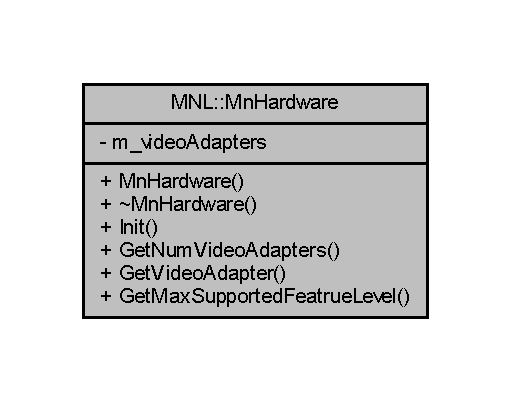
\includegraphics[width=245pt]{class_m_n_l_1_1_mn_hardware__coll__graph}
\end{center}
\end{figure}
\subsection*{Public 멤버 함수}
\begin{DoxyCompactItemize}
\item 
\hyperlink{class_m_n_l_1_1_mn_hardware_ad9270be0bcce91bf3a21b6cac432e713}{Mn\+Hardware} ()
\item 
\hyperlink{class_m_n_l_1_1_mn_hardware_a875d63cd3b81d293a3f38026816abb7e}{$\sim$\+Mn\+Hardware} ()
\item 
H\+R\+E\+S\+U\+LT \hyperlink{class_m_n_l_1_1_mn_hardware_a440da8664ff9470a3f5ef7f349a6d7f4}{Init} ()
\begin{DoxyCompactList}\small\item\em 장치 정보를 얻어와 초기화 한다. \end{DoxyCompactList}\item 
U\+I\+NT \hyperlink{class_m_n_l_1_1_mn_hardware_a4b614d4e29b4bd48f0d952f3ec707d12}{Get\+Num\+Video\+Adapters} () const
\begin{DoxyCompactList}\small\item\em 비디오 어댑터의 개수를 얻어온다. \end{DoxyCompactList}\item 
const \hyperlink{class_m_n_l_1_1_mn_video_adapter}{Mn\+Video\+Adapter} \hyperlink{class_m_n_l_1_1_mn_hardware_a84b1095acf9196e1bb0fe6a1f996b697}{Get\+Video\+Adapter} (U\+I\+NT index) const
\begin{DoxyCompactList}\small\item\em 컨테이너 내의 Mn\+Video\+Adapter를 얻어온다. \end{DoxyCompactList}\item 
D3\+D\+\_\+\+F\+E\+A\+T\+U\+R\+E\+\_\+\+L\+E\+V\+EL \hyperlink{class_m_n_l_1_1_mn_hardware_a8912748dc6e28ac992efb0282ee03ce5}{Get\+Max\+Supported\+Featrue\+Level} (U\+I\+NT adapter\+Index) const
\begin{DoxyCompactList}\small\item\em G\+P\+U가 지원하는 최대 피쳐 레벨을 얻는다. \end{DoxyCompactList}\end{DoxyCompactItemize}
\subsection*{Private 속성}
\begin{DoxyCompactItemize}
\item 
std\+::vector$<$ \hyperlink{class_m_n_l_1_1_mn_video_adapter}{Mn\+Video\+Adapter} $>$ \hyperlink{class_m_n_l_1_1_mn_hardware_a34ada79c31e979efd31bc7cee9c6e6e1}{m\+\_\+video\+Adapters}
\begin{DoxyCompactList}\small\item\em 초기화된 비디오 어댑터 장치가 저장되는 컨테이너 \end{DoxyCompactList}\end{DoxyCompactItemize}


\subsection{상세한 설명}
비디오 어댑터 및 디스플레이 장치 관리. 

\begin{DoxyAuthor}{작성자}
Akssus 
\end{DoxyAuthor}
\hypertarget{class_m_n_l_1_1_mn_video_adapter_개요}{}\subsection{개요}\label{class_m_n_l_1_1_mn_video_adapter_개요}
Mn\+Hardware는 Mn\+D3\+D\+Device를 생성하기 전 컴퓨터의 비디오 하드웨어 정보를 얻어오기 위한 객체이다.~\newline
~\newline
Mn\+Hardware는 Mn\+Video\+Adapter와 Mn\+Display\+Device를 통해 비디오 출력 관련 장치(비디오카드 및 모니터)의 정보를 저장, 관리한다.~\newline
~\newline
Mn\+Hardware는 Mn\+Display\+Device를 직접적으로 멤버로 가지지 않으며~\newline
~\newline
\hyperlink{class_m_n_l_1_1_mn_hardware}{Mn\+Hardware} -\/ \hyperlink{class_m_n_l_1_1_mn_video_adapter}{Mn\+Video\+Adapter} -\/ \hyperlink{class_m_n_l_1_1_mn_display_device}{Mn\+Display\+Device} ~\newline
1......n 1.....n ~\newline
~\newline
의 관계를 가진다.~\newline
이렇게 구조화된 이유는 한 대의 컴퓨터에서 여러개의 비디오카드를 가질 수 있고 (통상 한개지만) 각 비디오카드는 여러대의 모니터에 출력할 수 있기 때문이다.~\newline
특히 요즘은 듀얼 모니터 이상이 많아서 이에 대한 관리는 불가피한 듯 하다. 

Mn\+Hardware.\+h 파일의 27 번째 라인에서 정의되었습니다.



\subsection{생성자 \& 소멸자 문서화}
\mbox{\Hypertarget{class_m_n_l_1_1_mn_hardware_ad9270be0bcce91bf3a21b6cac432e713}\label{class_m_n_l_1_1_mn_hardware_ad9270be0bcce91bf3a21b6cac432e713}} 
\index{M\+N\+L\+::\+Mn\+Hardware@{M\+N\+L\+::\+Mn\+Hardware}!Mn\+Hardware@{Mn\+Hardware}}
\index{Mn\+Hardware@{Mn\+Hardware}!M\+N\+L\+::\+Mn\+Hardware@{M\+N\+L\+::\+Mn\+Hardware}}
\subsubsection{\texorpdfstring{Mn\+Hardware()}{MnHardware()}}
{\footnotesize\ttfamily Mn\+Hardware\+::\+Mn\+Hardware (\begin{DoxyParamCaption}{ }\end{DoxyParamCaption})}



Mn\+Hardware.\+cpp 파일의 7 번째 라인에서 정의되었습니다.

\mbox{\Hypertarget{class_m_n_l_1_1_mn_hardware_a875d63cd3b81d293a3f38026816abb7e}\label{class_m_n_l_1_1_mn_hardware_a875d63cd3b81d293a3f38026816abb7e}} 
\index{M\+N\+L\+::\+Mn\+Hardware@{M\+N\+L\+::\+Mn\+Hardware}!````~Mn\+Hardware@{$\sim$\+Mn\+Hardware}}
\index{````~Mn\+Hardware@{$\sim$\+Mn\+Hardware}!M\+N\+L\+::\+Mn\+Hardware@{M\+N\+L\+::\+Mn\+Hardware}}
\subsubsection{\texorpdfstring{$\sim$\+Mn\+Hardware()}{~MnHardware()}}
{\footnotesize\ttfamily Mn\+Hardware\+::$\sim$\+Mn\+Hardware (\begin{DoxyParamCaption}{ }\end{DoxyParamCaption})}



Mn\+Hardware.\+cpp 파일의 12 번째 라인에서 정의되었습니다.



\subsection{멤버 함수 문서화}
\mbox{\Hypertarget{class_m_n_l_1_1_mn_hardware_a8912748dc6e28ac992efb0282ee03ce5}\label{class_m_n_l_1_1_mn_hardware_a8912748dc6e28ac992efb0282ee03ce5}} 
\index{M\+N\+L\+::\+Mn\+Hardware@{M\+N\+L\+::\+Mn\+Hardware}!Get\+Max\+Supported\+Featrue\+Level@{Get\+Max\+Supported\+Featrue\+Level}}
\index{Get\+Max\+Supported\+Featrue\+Level@{Get\+Max\+Supported\+Featrue\+Level}!M\+N\+L\+::\+Mn\+Hardware@{M\+N\+L\+::\+Mn\+Hardware}}
\subsubsection{\texorpdfstring{Get\+Max\+Supported\+Featrue\+Level()}{GetMaxSupportedFeatrueLevel()}}
{\footnotesize\ttfamily D3\+D\+\_\+\+F\+E\+A\+T\+U\+R\+E\+\_\+\+L\+E\+V\+EL Mn\+Hardware\+::\+Get\+Max\+Supported\+Featrue\+Level (\begin{DoxyParamCaption}\item[{U\+I\+NT}]{adapter\+Index }\end{DoxyParamCaption}) const}



G\+P\+U가 지원하는 최대 피쳐 레벨을 얻는다. 

\begin{DoxyReturn}{반환값}
최소 D3\+D\+\_\+\+F\+E\+A\+T\+U\+R\+E\+\_\+\+L\+E\+V\+E\+L\+\_\+9\+\_\+1가 반환된다. 
\end{DoxyReturn}


Mn\+Hardware.\+cpp 파일의 62 번째 라인에서 정의되었습니다.

\mbox{\Hypertarget{class_m_n_l_1_1_mn_hardware_a4b614d4e29b4bd48f0d952f3ec707d12}\label{class_m_n_l_1_1_mn_hardware_a4b614d4e29b4bd48f0d952f3ec707d12}} 
\index{M\+N\+L\+::\+Mn\+Hardware@{M\+N\+L\+::\+Mn\+Hardware}!Get\+Num\+Video\+Adapters@{Get\+Num\+Video\+Adapters}}
\index{Get\+Num\+Video\+Adapters@{Get\+Num\+Video\+Adapters}!M\+N\+L\+::\+Mn\+Hardware@{M\+N\+L\+::\+Mn\+Hardware}}
\subsubsection{\texorpdfstring{Get\+Num\+Video\+Adapters()}{GetNumVideoAdapters()}}
{\footnotesize\ttfamily U\+I\+NT Mn\+Hardware\+::\+Get\+Num\+Video\+Adapters (\begin{DoxyParamCaption}{ }\end{DoxyParamCaption}) const}



비디오 어댑터의 개수를 얻어온다. 



Mn\+Hardware.\+cpp 파일의 53 번째 라인에서 정의되었습니다.

\mbox{\Hypertarget{class_m_n_l_1_1_mn_hardware_a84b1095acf9196e1bb0fe6a1f996b697}\label{class_m_n_l_1_1_mn_hardware_a84b1095acf9196e1bb0fe6a1f996b697}} 
\index{M\+N\+L\+::\+Mn\+Hardware@{M\+N\+L\+::\+Mn\+Hardware}!Get\+Video\+Adapter@{Get\+Video\+Adapter}}
\index{Get\+Video\+Adapter@{Get\+Video\+Adapter}!M\+N\+L\+::\+Mn\+Hardware@{M\+N\+L\+::\+Mn\+Hardware}}
\subsubsection{\texorpdfstring{Get\+Video\+Adapter()}{GetVideoAdapter()}}
{\footnotesize\ttfamily const \hyperlink{class_m_n_l_1_1_mn_video_adapter}{Mn\+Video\+Adapter} Mn\+Hardware\+::\+Get\+Video\+Adapter (\begin{DoxyParamCaption}\item[{U\+I\+NT}]{index }\end{DoxyParamCaption}) const}



컨테이너 내의 Mn\+Video\+Adapter를 얻어온다. 


\begin{DoxyParams}{매개변수}
{\em index} & 비디오 어댑터의 인덱스 \\
\hline
\end{DoxyParams}
\begin{DoxyWarning}{경고}
Out of index 동작시 크래시 발생 
\end{DoxyWarning}


Mn\+Hardware.\+cpp 파일의 57 번째 라인에서 정의되었습니다.

\mbox{\Hypertarget{class_m_n_l_1_1_mn_hardware_a440da8664ff9470a3f5ef7f349a6d7f4}\label{class_m_n_l_1_1_mn_hardware_a440da8664ff9470a3f5ef7f349a6d7f4}} 
\index{M\+N\+L\+::\+Mn\+Hardware@{M\+N\+L\+::\+Mn\+Hardware}!Init@{Init}}
\index{Init@{Init}!M\+N\+L\+::\+Mn\+Hardware@{M\+N\+L\+::\+Mn\+Hardware}}
\subsubsection{\texorpdfstring{Init()}{Init()}}
{\footnotesize\ttfamily H\+R\+E\+S\+U\+LT Mn\+Hardware\+::\+Init (\begin{DoxyParamCaption}{ }\end{DoxyParamCaption})}



장치 정보를 얻어와 초기화 한다. 

\begin{DoxyReturn}{반환값}
초기화 성공 여부. 
\end{DoxyReturn}


Mn\+Hardware.\+cpp 파일의 15 번째 라인에서 정의되었습니다.



\subsection{멤버 데이터 문서화}
\mbox{\Hypertarget{class_m_n_l_1_1_mn_hardware_a34ada79c31e979efd31bc7cee9c6e6e1}\label{class_m_n_l_1_1_mn_hardware_a34ada79c31e979efd31bc7cee9c6e6e1}} 
\index{M\+N\+L\+::\+Mn\+Hardware@{M\+N\+L\+::\+Mn\+Hardware}!m\+\_\+video\+Adapters@{m\+\_\+video\+Adapters}}
\index{m\+\_\+video\+Adapters@{m\+\_\+video\+Adapters}!M\+N\+L\+::\+Mn\+Hardware@{M\+N\+L\+::\+Mn\+Hardware}}
\subsubsection{\texorpdfstring{m\+\_\+video\+Adapters}{m\_videoAdapters}}
{\footnotesize\ttfamily std\+::vector$<$\hyperlink{class_m_n_l_1_1_mn_video_adapter}{Mn\+Video\+Adapter}$>$ M\+N\+L\+::\+Mn\+Hardware\+::m\+\_\+video\+Adapters\hspace{0.3cm}{\ttfamily [private]}}



초기화된 비디오 어댑터 장치가 저장되는 컨테이너 



Mn\+Hardware.\+h 파일의 58 번째 라인에서 정의되었습니다.



이 클래스에 대한 문서화 페이지는 다음의 파일들로부터 생성되었습니다.\+:\begin{DoxyCompactItemize}
\item 
Core/\hyperlink{_mn_hardware_8h}{Mn\+Hardware.\+h}\item 
Core/\hyperlink{_mn_hardware_8cpp}{Mn\+Hardware.\+cpp}\end{DoxyCompactItemize}

\hypertarget{class_m_n_l_1_1_mn_index_buffer}{}\section{M\+NL\+:\+:Mn\+Index\+Buffer 클래스 참조}
\label{class_m_n_l_1_1_mn_index_buffer}\index{M\+N\+L\+::\+Mn\+Index\+Buffer@{M\+N\+L\+::\+Mn\+Index\+Buffer}}


{\ttfamily \#include $<$Mn\+Index\+Buffer.\+h$>$}



M\+NL\+:\+:Mn\+Index\+Buffer에 대한 협력 다이어그램\+:\nopagebreak
\begin{figure}[H]
\begin{center}
\leavevmode
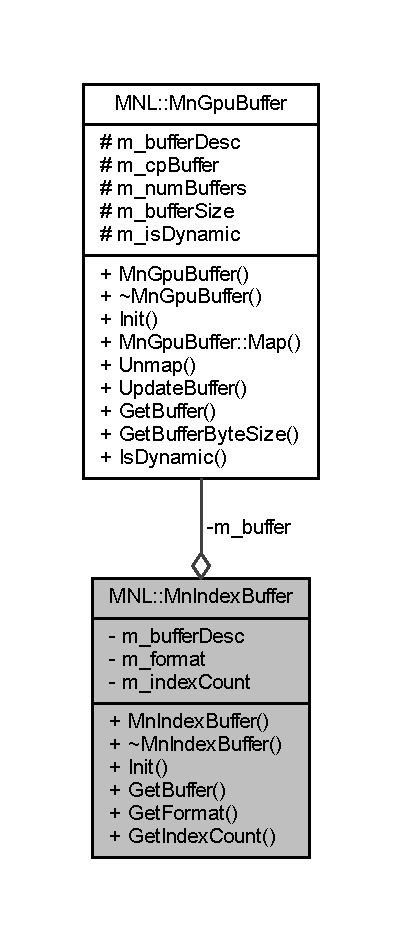
\includegraphics[width=193pt]{class_m_n_l_1_1_mn_index_buffer__coll__graph}
\end{center}
\end{figure}
\subsection*{Public 멤버 함수}
\begin{DoxyCompactItemize}
\item 
\hyperlink{class_m_n_l_1_1_mn_index_buffer_aaf66cb56ff4d0bed0b7ff1d784fff3f3}{Mn\+Index\+Buffer} ()
\item 
\hyperlink{class_m_n_l_1_1_mn_index_buffer_a6998f6b94aed324b016a85d47e9c83cc}{$\sim$\+Mn\+Index\+Buffer} ()
\item 
H\+R\+E\+S\+U\+LT \hyperlink{class_m_n_l_1_1_mn_index_buffer_ac5b1d0d65818b869497f265642fae509}{Init} (\hyperlink{namespace_m_n_l_a1eec210db8f309a4a9ac0d9658784c31}{C\+P\+D3\+D\+Device} cp\+Device, U\+I\+NT index\+Count, const D3\+D11\+\_\+\+S\+U\+B\+R\+E\+S\+O\+U\+R\+C\+E\+\_\+\+D\+A\+TA $\ast$initial\+Data)
\item 
const \hyperlink{namespace_m_n_l_aab9c90a8c27ac6410a9cc7cd89efeef1}{C\+P\+D3\+D\+Buffer} \hyperlink{class_m_n_l_1_1_mn_index_buffer_a5e0fe52326b487d0edfb30bb03b8b502}{Get\+Buffer} () const
\item 
const D\+X\+G\+I\+\_\+\+F\+O\+R\+M\+AT \hyperlink{class_m_n_l_1_1_mn_index_buffer_a65d7b963b3e376a0ab5fe6eb0cf946bd}{Get\+Format} () const
\item 
U\+I\+NT \hyperlink{class_m_n_l_1_1_mn_index_buffer_af4300e654b6bf847b4cba48b129cc664}{Get\+Index\+Count} () const
\end{DoxyCompactItemize}
\subsection*{Private 속성}
\begin{DoxyCompactItemize}
\item 
\hyperlink{class_m_n_l_1_1_mn_gpu_buffer}{Mn\+Gpu\+Buffer} \hyperlink{class_m_n_l_1_1_mn_index_buffer_a1dd52fcc71e02db79ee8b693c39423a8}{m\+\_\+buffer}
\item 
D3\+D11\+\_\+\+B\+U\+F\+F\+E\+R\+\_\+\+D\+E\+SC \hyperlink{class_m_n_l_1_1_mn_index_buffer_a36e716c1772bc9840bdd419bba026239}{m\+\_\+buffer\+Desc}
\item 
D\+X\+G\+I\+\_\+\+F\+O\+R\+M\+AT \hyperlink{class_m_n_l_1_1_mn_index_buffer_a426cdaa3bd2644dfc4880826cde9d333}{m\+\_\+format}
\item 
U\+I\+NT \hyperlink{class_m_n_l_1_1_mn_index_buffer_a273c18bf26ba770a8ebf008e6681720e}{m\+\_\+index\+Count}
\end{DoxyCompactItemize}


\subsection{상세한 설명}


Mn\+Index\+Buffer.\+h 파일의 8 번째 라인에서 정의되었습니다.



\subsection{생성자 \& 소멸자 문서화}
\mbox{\Hypertarget{class_m_n_l_1_1_mn_index_buffer_aaf66cb56ff4d0bed0b7ff1d784fff3f3}\label{class_m_n_l_1_1_mn_index_buffer_aaf66cb56ff4d0bed0b7ff1d784fff3f3}} 
\index{M\+N\+L\+::\+Mn\+Index\+Buffer@{M\+N\+L\+::\+Mn\+Index\+Buffer}!Mn\+Index\+Buffer@{Mn\+Index\+Buffer}}
\index{Mn\+Index\+Buffer@{Mn\+Index\+Buffer}!M\+N\+L\+::\+Mn\+Index\+Buffer@{M\+N\+L\+::\+Mn\+Index\+Buffer}}
\subsubsection{\texorpdfstring{Mn\+Index\+Buffer()}{MnIndexBuffer()}}
{\footnotesize\ttfamily Mn\+Index\+Buffer\+::\+Mn\+Index\+Buffer (\begin{DoxyParamCaption}{ }\end{DoxyParamCaption})}



Mn\+Index\+Buffer.\+cpp 파일의 6 번째 라인에서 정의되었습니다.

\mbox{\Hypertarget{class_m_n_l_1_1_mn_index_buffer_a6998f6b94aed324b016a85d47e9c83cc}\label{class_m_n_l_1_1_mn_index_buffer_a6998f6b94aed324b016a85d47e9c83cc}} 
\index{M\+N\+L\+::\+Mn\+Index\+Buffer@{M\+N\+L\+::\+Mn\+Index\+Buffer}!````~Mn\+Index\+Buffer@{$\sim$\+Mn\+Index\+Buffer}}
\index{````~Mn\+Index\+Buffer@{$\sim$\+Mn\+Index\+Buffer}!M\+N\+L\+::\+Mn\+Index\+Buffer@{M\+N\+L\+::\+Mn\+Index\+Buffer}}
\subsubsection{\texorpdfstring{$\sim$\+Mn\+Index\+Buffer()}{~MnIndexBuffer()}}
{\footnotesize\ttfamily Mn\+Index\+Buffer\+::$\sim$\+Mn\+Index\+Buffer (\begin{DoxyParamCaption}{ }\end{DoxyParamCaption})}



Mn\+Index\+Buffer.\+cpp 파일의 12 번째 라인에서 정의되었습니다.



\subsection{멤버 함수 문서화}
\mbox{\Hypertarget{class_m_n_l_1_1_mn_index_buffer_a5e0fe52326b487d0edfb30bb03b8b502}\label{class_m_n_l_1_1_mn_index_buffer_a5e0fe52326b487d0edfb30bb03b8b502}} 
\index{M\+N\+L\+::\+Mn\+Index\+Buffer@{M\+N\+L\+::\+Mn\+Index\+Buffer}!Get\+Buffer@{Get\+Buffer}}
\index{Get\+Buffer@{Get\+Buffer}!M\+N\+L\+::\+Mn\+Index\+Buffer@{M\+N\+L\+::\+Mn\+Index\+Buffer}}
\subsubsection{\texorpdfstring{Get\+Buffer()}{GetBuffer()}}
{\footnotesize\ttfamily const \hyperlink{namespace_m_n_l_aab9c90a8c27ac6410a9cc7cd89efeef1}{C\+P\+D3\+D\+Buffer} Mn\+Index\+Buffer\+::\+Get\+Buffer (\begin{DoxyParamCaption}{ }\end{DoxyParamCaption}) const}



Mn\+Index\+Buffer.\+cpp 파일의 37 번째 라인에서 정의되었습니다.

\mbox{\Hypertarget{class_m_n_l_1_1_mn_index_buffer_a65d7b963b3e376a0ab5fe6eb0cf946bd}\label{class_m_n_l_1_1_mn_index_buffer_a65d7b963b3e376a0ab5fe6eb0cf946bd}} 
\index{M\+N\+L\+::\+Mn\+Index\+Buffer@{M\+N\+L\+::\+Mn\+Index\+Buffer}!Get\+Format@{Get\+Format}}
\index{Get\+Format@{Get\+Format}!M\+N\+L\+::\+Mn\+Index\+Buffer@{M\+N\+L\+::\+Mn\+Index\+Buffer}}
\subsubsection{\texorpdfstring{Get\+Format()}{GetFormat()}}
{\footnotesize\ttfamily const D\+X\+G\+I\+\_\+\+F\+O\+R\+M\+AT Mn\+Index\+Buffer\+::\+Get\+Format (\begin{DoxyParamCaption}{ }\end{DoxyParamCaption}) const}



Mn\+Index\+Buffer.\+cpp 파일의 41 번째 라인에서 정의되었습니다.

\mbox{\Hypertarget{class_m_n_l_1_1_mn_index_buffer_af4300e654b6bf847b4cba48b129cc664}\label{class_m_n_l_1_1_mn_index_buffer_af4300e654b6bf847b4cba48b129cc664}} 
\index{M\+N\+L\+::\+Mn\+Index\+Buffer@{M\+N\+L\+::\+Mn\+Index\+Buffer}!Get\+Index\+Count@{Get\+Index\+Count}}
\index{Get\+Index\+Count@{Get\+Index\+Count}!M\+N\+L\+::\+Mn\+Index\+Buffer@{M\+N\+L\+::\+Mn\+Index\+Buffer}}
\subsubsection{\texorpdfstring{Get\+Index\+Count()}{GetIndexCount()}}
{\footnotesize\ttfamily U\+I\+NT Mn\+Index\+Buffer\+::\+Get\+Index\+Count (\begin{DoxyParamCaption}{ }\end{DoxyParamCaption}) const}



Mn\+Index\+Buffer.\+cpp 파일의 45 번째 라인에서 정의되었습니다.

\mbox{\Hypertarget{class_m_n_l_1_1_mn_index_buffer_ac5b1d0d65818b869497f265642fae509}\label{class_m_n_l_1_1_mn_index_buffer_ac5b1d0d65818b869497f265642fae509}} 
\index{M\+N\+L\+::\+Mn\+Index\+Buffer@{M\+N\+L\+::\+Mn\+Index\+Buffer}!Init@{Init}}
\index{Init@{Init}!M\+N\+L\+::\+Mn\+Index\+Buffer@{M\+N\+L\+::\+Mn\+Index\+Buffer}}
\subsubsection{\texorpdfstring{Init()}{Init()}}
{\footnotesize\ttfamily H\+R\+E\+S\+U\+LT Mn\+Index\+Buffer\+::\+Init (\begin{DoxyParamCaption}\item[{\hyperlink{namespace_m_n_l_a1eec210db8f309a4a9ac0d9658784c31}{C\+P\+D3\+D\+Device}}]{cp\+Device,  }\item[{U\+I\+NT}]{index\+Count,  }\item[{const D3\+D11\+\_\+\+S\+U\+B\+R\+E\+S\+O\+U\+R\+C\+E\+\_\+\+D\+A\+TA $\ast$}]{initial\+Data }\end{DoxyParamCaption})}



Mn\+Index\+Buffer.\+cpp 파일의 16 번째 라인에서 정의되었습니다.



\subsection{멤버 데이터 문서화}
\mbox{\Hypertarget{class_m_n_l_1_1_mn_index_buffer_a1dd52fcc71e02db79ee8b693c39423a8}\label{class_m_n_l_1_1_mn_index_buffer_a1dd52fcc71e02db79ee8b693c39423a8}} 
\index{M\+N\+L\+::\+Mn\+Index\+Buffer@{M\+N\+L\+::\+Mn\+Index\+Buffer}!m\+\_\+buffer@{m\+\_\+buffer}}
\index{m\+\_\+buffer@{m\+\_\+buffer}!M\+N\+L\+::\+Mn\+Index\+Buffer@{M\+N\+L\+::\+Mn\+Index\+Buffer}}
\subsubsection{\texorpdfstring{m\+\_\+buffer}{m\_buffer}}
{\footnotesize\ttfamily \hyperlink{class_m_n_l_1_1_mn_gpu_buffer}{Mn\+Gpu\+Buffer} M\+N\+L\+::\+Mn\+Index\+Buffer\+::m\+\_\+buffer\hspace{0.3cm}{\ttfamily [private]}}



Mn\+Index\+Buffer.\+h 파일의 23 번째 라인에서 정의되었습니다.

\mbox{\Hypertarget{class_m_n_l_1_1_mn_index_buffer_a36e716c1772bc9840bdd419bba026239}\label{class_m_n_l_1_1_mn_index_buffer_a36e716c1772bc9840bdd419bba026239}} 
\index{M\+N\+L\+::\+Mn\+Index\+Buffer@{M\+N\+L\+::\+Mn\+Index\+Buffer}!m\+\_\+buffer\+Desc@{m\+\_\+buffer\+Desc}}
\index{m\+\_\+buffer\+Desc@{m\+\_\+buffer\+Desc}!M\+N\+L\+::\+Mn\+Index\+Buffer@{M\+N\+L\+::\+Mn\+Index\+Buffer}}
\subsubsection{\texorpdfstring{m\+\_\+buffer\+Desc}{m\_bufferDesc}}
{\footnotesize\ttfamily D3\+D11\+\_\+\+B\+U\+F\+F\+E\+R\+\_\+\+D\+E\+SC M\+N\+L\+::\+Mn\+Index\+Buffer\+::m\+\_\+buffer\+Desc\hspace{0.3cm}{\ttfamily [private]}}



Mn\+Index\+Buffer.\+h 파일의 24 번째 라인에서 정의되었습니다.

\mbox{\Hypertarget{class_m_n_l_1_1_mn_index_buffer_a426cdaa3bd2644dfc4880826cde9d333}\label{class_m_n_l_1_1_mn_index_buffer_a426cdaa3bd2644dfc4880826cde9d333}} 
\index{M\+N\+L\+::\+Mn\+Index\+Buffer@{M\+N\+L\+::\+Mn\+Index\+Buffer}!m\+\_\+format@{m\+\_\+format}}
\index{m\+\_\+format@{m\+\_\+format}!M\+N\+L\+::\+Mn\+Index\+Buffer@{M\+N\+L\+::\+Mn\+Index\+Buffer}}
\subsubsection{\texorpdfstring{m\+\_\+format}{m\_format}}
{\footnotesize\ttfamily D\+X\+G\+I\+\_\+\+F\+O\+R\+M\+AT M\+N\+L\+::\+Mn\+Index\+Buffer\+::m\+\_\+format\hspace{0.3cm}{\ttfamily [private]}}



Mn\+Index\+Buffer.\+h 파일의 25 번째 라인에서 정의되었습니다.

\mbox{\Hypertarget{class_m_n_l_1_1_mn_index_buffer_a273c18bf26ba770a8ebf008e6681720e}\label{class_m_n_l_1_1_mn_index_buffer_a273c18bf26ba770a8ebf008e6681720e}} 
\index{M\+N\+L\+::\+Mn\+Index\+Buffer@{M\+N\+L\+::\+Mn\+Index\+Buffer}!m\+\_\+index\+Count@{m\+\_\+index\+Count}}
\index{m\+\_\+index\+Count@{m\+\_\+index\+Count}!M\+N\+L\+::\+Mn\+Index\+Buffer@{M\+N\+L\+::\+Mn\+Index\+Buffer}}
\subsubsection{\texorpdfstring{m\+\_\+index\+Count}{m\_indexCount}}
{\footnotesize\ttfamily U\+I\+NT M\+N\+L\+::\+Mn\+Index\+Buffer\+::m\+\_\+index\+Count\hspace{0.3cm}{\ttfamily [private]}}



Mn\+Index\+Buffer.\+h 파일의 26 번째 라인에서 정의되었습니다.



이 클래스에 대한 문서화 페이지는 다음의 파일들로부터 생성되었습니다.\+:\begin{DoxyCompactItemize}
\item 
Core/\hyperlink{_mn_index_buffer_8h}{Mn\+Index\+Buffer.\+h}\item 
Core/\hyperlink{_mn_index_buffer_8cpp}{Mn\+Index\+Buffer.\+cpp}\end{DoxyCompactItemize}

\hypertarget{class_m_n_l_1_1_mn_input_element}{}\section{M\+NL\+:\+:Mn\+Input\+Element 클래스 참조}
\label{class_m_n_l_1_1_mn_input_element}\index{M\+N\+L\+::\+Mn\+Input\+Element@{M\+N\+L\+::\+Mn\+Input\+Element}}


{\ttfamily \#include $<$Mn\+Input\+Element.\+h$>$}



M\+NL\+:\+:Mn\+Input\+Element에 대한 협력 다이어그램\+:\nopagebreak
\begin{figure}[H]
\begin{center}
\leavevmode
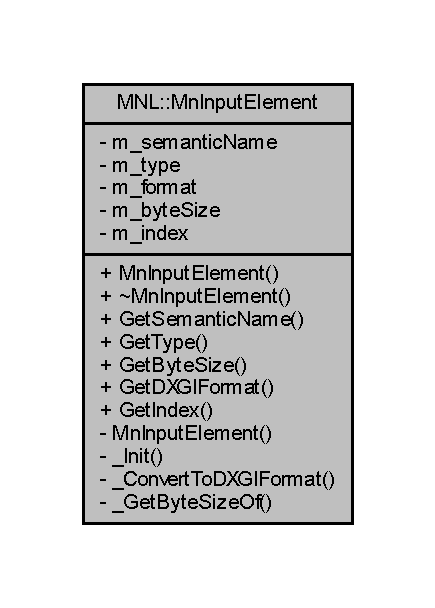
\includegraphics[width=209pt]{class_m_n_l_1_1_mn_input_element__coll__graph}
\end{center}
\end{figure}
\subsection*{Public 멤버 함수}
\begin{DoxyCompactItemize}
\item 
\hyperlink{class_m_n_l_1_1_mn_input_element_a0a2c66ec037982166078a9d6d2318aa2}{Mn\+Input\+Element} (std\+::string semantic\+Name, const \hyperlink{namespace_m_n_l_a8605571a36b2bb477280767d71fe6f9e}{Mn\+Input\+Element\+Type} \&input\+Element\+Type, U\+I\+NT index)
\item 
\hyperlink{class_m_n_l_1_1_mn_input_element_a42dc56f9038c224c826dafac6257fa29}{$\sim$\+Mn\+Input\+Element} ()
\item 
const std\+::string \& \hyperlink{class_m_n_l_1_1_mn_input_element_a6aa08fd62581e1eddc7e632de0bd9564}{Get\+Semantic\+Name} () const
\item 
\hyperlink{namespace_m_n_l_a8605571a36b2bb477280767d71fe6f9e}{Mn\+Input\+Element\+Type} \hyperlink{class_m_n_l_1_1_mn_input_element_a21970e5ba0187033e34bec04da162741}{Get\+Type} () const
\item 
U\+I\+NT \hyperlink{class_m_n_l_1_1_mn_input_element_a1bdc917e5920941e913048e6a39eaa48}{Get\+Byte\+Size} () const
\item 
D\+X\+G\+I\+\_\+\+F\+O\+R\+M\+AT \hyperlink{class_m_n_l_1_1_mn_input_element_ac9856490638cc98b23e533782107e4a6}{Get\+D\+X\+G\+I\+Format} () const
\item 
U\+I\+NT \hyperlink{class_m_n_l_1_1_mn_input_element_a314bdce70c4781632737c247c040f014}{Get\+Index} () const
\end{DoxyCompactItemize}
\subsection*{Private 멤버 함수}
\begin{DoxyCompactItemize}
\item 
\hyperlink{class_m_n_l_1_1_mn_input_element_a3ac0bac42c3d2d6e1edf29f28df54190}{Mn\+Input\+Element} ()
\item 
bool \hyperlink{class_m_n_l_1_1_mn_input_element_aae3dcc9e65bf14d53d7fc92803eb20da}{\+\_\+\+Init} (std\+::string semantic\+Name, const \hyperlink{namespace_m_n_l_a8605571a36b2bb477280767d71fe6f9e}{Mn\+Input\+Element\+Type} \&input\+Element\+Type, U\+I\+NT index)
\item 
D\+X\+G\+I\+\_\+\+F\+O\+R\+M\+AT \hyperlink{class_m_n_l_1_1_mn_input_element_adae99b575f381bd5241f4d9df7c8d56b}{\+\_\+\+Convert\+To\+D\+X\+G\+I\+Format} (const \hyperlink{namespace_m_n_l_a8605571a36b2bb477280767d71fe6f9e}{Mn\+Input\+Element\+Type} \&input\+Element\+Type)
\item 
U\+I\+NT \hyperlink{class_m_n_l_1_1_mn_input_element_ad84bf259c4a3674490f5b789b4f21e67}{\+\_\+\+Get\+Byte\+Size\+Of} (const \hyperlink{namespace_m_n_l_a8605571a36b2bb477280767d71fe6f9e}{Mn\+Input\+Element\+Type} \&input\+Element\+Type)
\end{DoxyCompactItemize}
\subsection*{Private 속성}
\begin{DoxyCompactItemize}
\item 
std\+::string \hyperlink{class_m_n_l_1_1_mn_input_element_add6831c8eac59037aea8ab7f0ad590ca}{m\+\_\+semantic\+Name}
\item 
\hyperlink{namespace_m_n_l_a8605571a36b2bb477280767d71fe6f9e}{Mn\+Input\+Element\+Type} \hyperlink{class_m_n_l_1_1_mn_input_element_a8c81b40be5e4108e7473b0589e0da8f5}{m\+\_\+type}
\item 
D\+X\+G\+I\+\_\+\+F\+O\+R\+M\+AT \hyperlink{class_m_n_l_1_1_mn_input_element_a6c247125236a7166fdbf1a7dca654f51}{m\+\_\+format}
\item 
U\+I\+NT \hyperlink{class_m_n_l_1_1_mn_input_element_a8a93b5979d9bc94600a979811532366f}{m\+\_\+byte\+Size}
\item 
U\+I\+NT \hyperlink{class_m_n_l_1_1_mn_input_element_ad75d411d62b10a84eb494c948fee379d}{m\+\_\+index}
\end{DoxyCompactItemize}


\subsection{상세한 설명}


Mn\+Input\+Element.\+h 파일의 20 번째 라인에서 정의되었습니다.



\subsection{생성자 \& 소멸자 문서화}
\mbox{\Hypertarget{class_m_n_l_1_1_mn_input_element_a0a2c66ec037982166078a9d6d2318aa2}\label{class_m_n_l_1_1_mn_input_element_a0a2c66ec037982166078a9d6d2318aa2}} 
\index{M\+N\+L\+::\+Mn\+Input\+Element@{M\+N\+L\+::\+Mn\+Input\+Element}!Mn\+Input\+Element@{Mn\+Input\+Element}}
\index{Mn\+Input\+Element@{Mn\+Input\+Element}!M\+N\+L\+::\+Mn\+Input\+Element@{M\+N\+L\+::\+Mn\+Input\+Element}}
\subsubsection{\texorpdfstring{Mn\+Input\+Element()}{MnInputElement()}\hspace{0.1cm}{\footnotesize\ttfamily [1/2]}}
{\footnotesize\ttfamily Mn\+Input\+Element\+::\+Mn\+Input\+Element (\begin{DoxyParamCaption}\item[{std\+::string}]{semantic\+Name,  }\item[{const \hyperlink{namespace_m_n_l_a8605571a36b2bb477280767d71fe6f9e}{Mn\+Input\+Element\+Type} \&}]{input\+Element\+Type,  }\item[{U\+I\+NT}]{index }\end{DoxyParamCaption})}



Mn\+Input\+Element.\+cpp 파일의 11 번째 라인에서 정의되었습니다.

\mbox{\Hypertarget{class_m_n_l_1_1_mn_input_element_a42dc56f9038c224c826dafac6257fa29}\label{class_m_n_l_1_1_mn_input_element_a42dc56f9038c224c826dafac6257fa29}} 
\index{M\+N\+L\+::\+Mn\+Input\+Element@{M\+N\+L\+::\+Mn\+Input\+Element}!````~Mn\+Input\+Element@{$\sim$\+Mn\+Input\+Element}}
\index{````~Mn\+Input\+Element@{$\sim$\+Mn\+Input\+Element}!M\+N\+L\+::\+Mn\+Input\+Element@{M\+N\+L\+::\+Mn\+Input\+Element}}
\subsubsection{\texorpdfstring{$\sim$\+Mn\+Input\+Element()}{~MnInputElement()}}
{\footnotesize\ttfamily Mn\+Input\+Element\+::$\sim$\+Mn\+Input\+Element (\begin{DoxyParamCaption}{ }\end{DoxyParamCaption})}



Mn\+Input\+Element.\+cpp 파일의 18 번째 라인에서 정의되었습니다.

\mbox{\Hypertarget{class_m_n_l_1_1_mn_input_element_a3ac0bac42c3d2d6e1edf29f28df54190}\label{class_m_n_l_1_1_mn_input_element_a3ac0bac42c3d2d6e1edf29f28df54190}} 
\index{M\+N\+L\+::\+Mn\+Input\+Element@{M\+N\+L\+::\+Mn\+Input\+Element}!Mn\+Input\+Element@{Mn\+Input\+Element}}
\index{Mn\+Input\+Element@{Mn\+Input\+Element}!M\+N\+L\+::\+Mn\+Input\+Element@{M\+N\+L\+::\+Mn\+Input\+Element}}
\subsubsection{\texorpdfstring{Mn\+Input\+Element()}{MnInputElement()}\hspace{0.1cm}{\footnotesize\ttfamily [2/2]}}
{\footnotesize\ttfamily Mn\+Input\+Element\+::\+Mn\+Input\+Element (\begin{DoxyParamCaption}{ }\end{DoxyParamCaption})\hspace{0.3cm}{\ttfamily [private]}}



Mn\+Input\+Element.\+cpp 파일의 5 번째 라인에서 정의되었습니다.



\subsection{멤버 함수 문서화}
\mbox{\Hypertarget{class_m_n_l_1_1_mn_input_element_adae99b575f381bd5241f4d9df7c8d56b}\label{class_m_n_l_1_1_mn_input_element_adae99b575f381bd5241f4d9df7c8d56b}} 
\index{M\+N\+L\+::\+Mn\+Input\+Element@{M\+N\+L\+::\+Mn\+Input\+Element}!\+\_\+\+Convert\+To\+D\+X\+G\+I\+Format@{\+\_\+\+Convert\+To\+D\+X\+G\+I\+Format}}
\index{\+\_\+\+Convert\+To\+D\+X\+G\+I\+Format@{\+\_\+\+Convert\+To\+D\+X\+G\+I\+Format}!M\+N\+L\+::\+Mn\+Input\+Element@{M\+N\+L\+::\+Mn\+Input\+Element}}
\subsubsection{\texorpdfstring{\+\_\+\+Convert\+To\+D\+X\+G\+I\+Format()}{\_ConvertToDXGIFormat()}}
{\footnotesize\ttfamily D\+X\+G\+I\+\_\+\+F\+O\+R\+M\+AT Mn\+Input\+Element\+::\+\_\+\+Convert\+To\+D\+X\+G\+I\+Format (\begin{DoxyParamCaption}\item[{const \hyperlink{namespace_m_n_l_a8605571a36b2bb477280767d71fe6f9e}{Mn\+Input\+Element\+Type} \&}]{input\+Element\+Type }\end{DoxyParamCaption})\hspace{0.3cm}{\ttfamily [private]}}



Mn\+Input\+Element.\+cpp 파일의 61 번째 라인에서 정의되었습니다.

\mbox{\Hypertarget{class_m_n_l_1_1_mn_input_element_ad84bf259c4a3674490f5b789b4f21e67}\label{class_m_n_l_1_1_mn_input_element_ad84bf259c4a3674490f5b789b4f21e67}} 
\index{M\+N\+L\+::\+Mn\+Input\+Element@{M\+N\+L\+::\+Mn\+Input\+Element}!\+\_\+\+Get\+Byte\+Size\+Of@{\+\_\+\+Get\+Byte\+Size\+Of}}
\index{\+\_\+\+Get\+Byte\+Size\+Of@{\+\_\+\+Get\+Byte\+Size\+Of}!M\+N\+L\+::\+Mn\+Input\+Element@{M\+N\+L\+::\+Mn\+Input\+Element}}
\subsubsection{\texorpdfstring{\+\_\+\+Get\+Byte\+Size\+Of()}{\_GetByteSizeOf()}}
{\footnotesize\ttfamily U\+I\+NT Mn\+Input\+Element\+::\+\_\+\+Get\+Byte\+Size\+Of (\begin{DoxyParamCaption}\item[{const \hyperlink{namespace_m_n_l_a8605571a36b2bb477280767d71fe6f9e}{Mn\+Input\+Element\+Type} \&}]{input\+Element\+Type }\end{DoxyParamCaption})\hspace{0.3cm}{\ttfamily [private]}}



Mn\+Input\+Element.\+cpp 파일의 81 번째 라인에서 정의되었습니다.

\mbox{\Hypertarget{class_m_n_l_1_1_mn_input_element_aae3dcc9e65bf14d53d7fc92803eb20da}\label{class_m_n_l_1_1_mn_input_element_aae3dcc9e65bf14d53d7fc92803eb20da}} 
\index{M\+N\+L\+::\+Mn\+Input\+Element@{M\+N\+L\+::\+Mn\+Input\+Element}!\+\_\+\+Init@{\+\_\+\+Init}}
\index{\+\_\+\+Init@{\+\_\+\+Init}!M\+N\+L\+::\+Mn\+Input\+Element@{M\+N\+L\+::\+Mn\+Input\+Element}}
\subsubsection{\texorpdfstring{\+\_\+\+Init()}{\_Init()}}
{\footnotesize\ttfamily bool Mn\+Input\+Element\+::\+\_\+\+Init (\begin{DoxyParamCaption}\item[{std\+::string}]{semantic\+Name,  }\item[{const \hyperlink{namespace_m_n_l_a8605571a36b2bb477280767d71fe6f9e}{Mn\+Input\+Element\+Type} \&}]{input\+Element\+Type,  }\item[{U\+I\+NT}]{index }\end{DoxyParamCaption})\hspace{0.3cm}{\ttfamily [private]}}



Mn\+Input\+Element.\+cpp 파일의 22 번째 라인에서 정의되었습니다.

\mbox{\Hypertarget{class_m_n_l_1_1_mn_input_element_a1bdc917e5920941e913048e6a39eaa48}\label{class_m_n_l_1_1_mn_input_element_a1bdc917e5920941e913048e6a39eaa48}} 
\index{M\+N\+L\+::\+Mn\+Input\+Element@{M\+N\+L\+::\+Mn\+Input\+Element}!Get\+Byte\+Size@{Get\+Byte\+Size}}
\index{Get\+Byte\+Size@{Get\+Byte\+Size}!M\+N\+L\+::\+Mn\+Input\+Element@{M\+N\+L\+::\+Mn\+Input\+Element}}
\subsubsection{\texorpdfstring{Get\+Byte\+Size()}{GetByteSize()}}
{\footnotesize\ttfamily U\+I\+NT Mn\+Input\+Element\+::\+Get\+Byte\+Size (\begin{DoxyParamCaption}{ }\end{DoxyParamCaption}) const}



Mn\+Input\+Element.\+cpp 파일의 47 번째 라인에서 정의되었습니다.

\mbox{\Hypertarget{class_m_n_l_1_1_mn_input_element_ac9856490638cc98b23e533782107e4a6}\label{class_m_n_l_1_1_mn_input_element_ac9856490638cc98b23e533782107e4a6}} 
\index{M\+N\+L\+::\+Mn\+Input\+Element@{M\+N\+L\+::\+Mn\+Input\+Element}!Get\+D\+X\+G\+I\+Format@{Get\+D\+X\+G\+I\+Format}}
\index{Get\+D\+X\+G\+I\+Format@{Get\+D\+X\+G\+I\+Format}!M\+N\+L\+::\+Mn\+Input\+Element@{M\+N\+L\+::\+Mn\+Input\+Element}}
\subsubsection{\texorpdfstring{Get\+D\+X\+G\+I\+Format()}{GetDXGIFormat()}}
{\footnotesize\ttfamily D\+X\+G\+I\+\_\+\+F\+O\+R\+M\+AT Mn\+Input\+Element\+::\+Get\+D\+X\+G\+I\+Format (\begin{DoxyParamCaption}{ }\end{DoxyParamCaption}) const}



Mn\+Input\+Element.\+cpp 파일의 51 번째 라인에서 정의되었습니다.

\mbox{\Hypertarget{class_m_n_l_1_1_mn_input_element_a314bdce70c4781632737c247c040f014}\label{class_m_n_l_1_1_mn_input_element_a314bdce70c4781632737c247c040f014}} 
\index{M\+N\+L\+::\+Mn\+Input\+Element@{M\+N\+L\+::\+Mn\+Input\+Element}!Get\+Index@{Get\+Index}}
\index{Get\+Index@{Get\+Index}!M\+N\+L\+::\+Mn\+Input\+Element@{M\+N\+L\+::\+Mn\+Input\+Element}}
\subsubsection{\texorpdfstring{Get\+Index()}{GetIndex()}}
{\footnotesize\ttfamily U\+I\+NT Mn\+Input\+Element\+::\+Get\+Index (\begin{DoxyParamCaption}{ }\end{DoxyParamCaption}) const}



Mn\+Input\+Element.\+cpp 파일의 56 번째 라인에서 정의되었습니다.

\mbox{\Hypertarget{class_m_n_l_1_1_mn_input_element_a6aa08fd62581e1eddc7e632de0bd9564}\label{class_m_n_l_1_1_mn_input_element_a6aa08fd62581e1eddc7e632de0bd9564}} 
\index{M\+N\+L\+::\+Mn\+Input\+Element@{M\+N\+L\+::\+Mn\+Input\+Element}!Get\+Semantic\+Name@{Get\+Semantic\+Name}}
\index{Get\+Semantic\+Name@{Get\+Semantic\+Name}!M\+N\+L\+::\+Mn\+Input\+Element@{M\+N\+L\+::\+Mn\+Input\+Element}}
\subsubsection{\texorpdfstring{Get\+Semantic\+Name()}{GetSemanticName()}}
{\footnotesize\ttfamily const std\+::string \& Mn\+Input\+Element\+::\+Get\+Semantic\+Name (\begin{DoxyParamCaption}{ }\end{DoxyParamCaption}) const}



Mn\+Input\+Element.\+cpp 파일의 39 번째 라인에서 정의되었습니다.

\mbox{\Hypertarget{class_m_n_l_1_1_mn_input_element_a21970e5ba0187033e34bec04da162741}\label{class_m_n_l_1_1_mn_input_element_a21970e5ba0187033e34bec04da162741}} 
\index{M\+N\+L\+::\+Mn\+Input\+Element@{M\+N\+L\+::\+Mn\+Input\+Element}!Get\+Type@{Get\+Type}}
\index{Get\+Type@{Get\+Type}!M\+N\+L\+::\+Mn\+Input\+Element@{M\+N\+L\+::\+Mn\+Input\+Element}}
\subsubsection{\texorpdfstring{Get\+Type()}{GetType()}}
{\footnotesize\ttfamily \hyperlink{namespace_m_n_l_a8605571a36b2bb477280767d71fe6f9e}{Mn\+Input\+Element\+Type} Mn\+Input\+Element\+::\+Get\+Type (\begin{DoxyParamCaption}{ }\end{DoxyParamCaption}) const}



Mn\+Input\+Element.\+cpp 파일의 43 번째 라인에서 정의되었습니다.



\subsection{멤버 데이터 문서화}
\mbox{\Hypertarget{class_m_n_l_1_1_mn_input_element_a8a93b5979d9bc94600a979811532366f}\label{class_m_n_l_1_1_mn_input_element_a8a93b5979d9bc94600a979811532366f}} 
\index{M\+N\+L\+::\+Mn\+Input\+Element@{M\+N\+L\+::\+Mn\+Input\+Element}!m\+\_\+byte\+Size@{m\+\_\+byte\+Size}}
\index{m\+\_\+byte\+Size@{m\+\_\+byte\+Size}!M\+N\+L\+::\+Mn\+Input\+Element@{M\+N\+L\+::\+Mn\+Input\+Element}}
\subsubsection{\texorpdfstring{m\+\_\+byte\+Size}{m\_byteSize}}
{\footnotesize\ttfamily U\+I\+NT M\+N\+L\+::\+Mn\+Input\+Element\+::m\+\_\+byte\+Size\hspace{0.3cm}{\ttfamily [private]}}



Mn\+Input\+Element.\+h 파일의 42 번째 라인에서 정의되었습니다.

\mbox{\Hypertarget{class_m_n_l_1_1_mn_input_element_a6c247125236a7166fdbf1a7dca654f51}\label{class_m_n_l_1_1_mn_input_element_a6c247125236a7166fdbf1a7dca654f51}} 
\index{M\+N\+L\+::\+Mn\+Input\+Element@{M\+N\+L\+::\+Mn\+Input\+Element}!m\+\_\+format@{m\+\_\+format}}
\index{m\+\_\+format@{m\+\_\+format}!M\+N\+L\+::\+Mn\+Input\+Element@{M\+N\+L\+::\+Mn\+Input\+Element}}
\subsubsection{\texorpdfstring{m\+\_\+format}{m\_format}}
{\footnotesize\ttfamily D\+X\+G\+I\+\_\+\+F\+O\+R\+M\+AT M\+N\+L\+::\+Mn\+Input\+Element\+::m\+\_\+format\hspace{0.3cm}{\ttfamily [private]}}



Mn\+Input\+Element.\+h 파일의 41 번째 라인에서 정의되었습니다.

\mbox{\Hypertarget{class_m_n_l_1_1_mn_input_element_ad75d411d62b10a84eb494c948fee379d}\label{class_m_n_l_1_1_mn_input_element_ad75d411d62b10a84eb494c948fee379d}} 
\index{M\+N\+L\+::\+Mn\+Input\+Element@{M\+N\+L\+::\+Mn\+Input\+Element}!m\+\_\+index@{m\+\_\+index}}
\index{m\+\_\+index@{m\+\_\+index}!M\+N\+L\+::\+Mn\+Input\+Element@{M\+N\+L\+::\+Mn\+Input\+Element}}
\subsubsection{\texorpdfstring{m\+\_\+index}{m\_index}}
{\footnotesize\ttfamily U\+I\+NT M\+N\+L\+::\+Mn\+Input\+Element\+::m\+\_\+index\hspace{0.3cm}{\ttfamily [private]}}



Mn\+Input\+Element.\+h 파일의 43 번째 라인에서 정의되었습니다.

\mbox{\Hypertarget{class_m_n_l_1_1_mn_input_element_add6831c8eac59037aea8ab7f0ad590ca}\label{class_m_n_l_1_1_mn_input_element_add6831c8eac59037aea8ab7f0ad590ca}} 
\index{M\+N\+L\+::\+Mn\+Input\+Element@{M\+N\+L\+::\+Mn\+Input\+Element}!m\+\_\+semantic\+Name@{m\+\_\+semantic\+Name}}
\index{m\+\_\+semantic\+Name@{m\+\_\+semantic\+Name}!M\+N\+L\+::\+Mn\+Input\+Element@{M\+N\+L\+::\+Mn\+Input\+Element}}
\subsubsection{\texorpdfstring{m\+\_\+semantic\+Name}{m\_semanticName}}
{\footnotesize\ttfamily std\+::string M\+N\+L\+::\+Mn\+Input\+Element\+::m\+\_\+semantic\+Name\hspace{0.3cm}{\ttfamily [private]}}



Mn\+Input\+Element.\+h 파일의 39 번째 라인에서 정의되었습니다.

\mbox{\Hypertarget{class_m_n_l_1_1_mn_input_element_a8c81b40be5e4108e7473b0589e0da8f5}\label{class_m_n_l_1_1_mn_input_element_a8c81b40be5e4108e7473b0589e0da8f5}} 
\index{M\+N\+L\+::\+Mn\+Input\+Element@{M\+N\+L\+::\+Mn\+Input\+Element}!m\+\_\+type@{m\+\_\+type}}
\index{m\+\_\+type@{m\+\_\+type}!M\+N\+L\+::\+Mn\+Input\+Element@{M\+N\+L\+::\+Mn\+Input\+Element}}
\subsubsection{\texorpdfstring{m\+\_\+type}{m\_type}}
{\footnotesize\ttfamily \hyperlink{namespace_m_n_l_a8605571a36b2bb477280767d71fe6f9e}{Mn\+Input\+Element\+Type} M\+N\+L\+::\+Mn\+Input\+Element\+::m\+\_\+type\hspace{0.3cm}{\ttfamily [private]}}



Mn\+Input\+Element.\+h 파일의 40 번째 라인에서 정의되었습니다.



이 클래스에 대한 문서화 페이지는 다음의 파일들로부터 생성되었습니다.\+:\begin{DoxyCompactItemize}
\item 
Core/\hyperlink{_mn_input_element_8h}{Mn\+Input\+Element.\+h}\item 
Core/\hyperlink{_mn_input_element_8cpp}{Mn\+Input\+Element.\+cpp}\end{DoxyCompactItemize}

\hypertarget{class_m_n_l_1_1_mn_input_layout}{}\section{M\+NL\+:\+:Mn\+Input\+Layout 클래스 참조}
\label{class_m_n_l_1_1_mn_input_layout}\index{M\+N\+L\+::\+Mn\+Input\+Layout@{M\+N\+L\+::\+Mn\+Input\+Layout}}


{\ttfamily \#include $<$Mn\+Input\+Layout.\+h$>$}



M\+NL\+:\+:Mn\+Input\+Layout에 대한 협력 다이어그램\+:\nopagebreak
\begin{figure}[H]
\begin{center}
\leavevmode
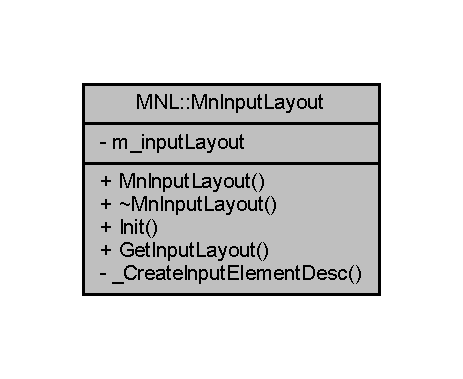
\includegraphics[width=222pt]{class_m_n_l_1_1_mn_input_layout__coll__graph}
\end{center}
\end{figure}
\subsection*{Public 멤버 함수}
\begin{DoxyCompactItemize}
\item 
\hyperlink{class_m_n_l_1_1_mn_input_layout_a937cd608980a37244885b81118c83a9a}{Mn\+Input\+Layout} ()
\item 
\hyperlink{class_m_n_l_1_1_mn_input_layout_a81a10cb04e3ee8bca95d1585feddf7e3}{$\sim$\+Mn\+Input\+Layout} ()
\item 
H\+R\+E\+S\+U\+LT \hyperlink{class_m_n_l_1_1_mn_input_layout_a7f97321379e253c8ae1c43c15a02f356}{Init} (\hyperlink{namespace_m_n_l_a1eec210db8f309a4a9ac0d9658784c31}{C\+P\+D3\+D\+Device} cp\+D3\+D\+Device, const std\+::shared\+\_\+ptr$<$ \hyperlink{class_m_n_l_1_1_mn_custom_vertex_type}{Mn\+Custom\+Vertex\+Type} $>$ p\+Custom\+Vertex\+Type, const std\+::shared\+\_\+ptr$<$ \hyperlink{class_m_n_l_1_1_mn_vertex_shader}{Mn\+Vertex\+Shader} $>$ p\+Vertex\+Shader)
\item 
\hyperlink{namespace_m_n_l_aec7a2a132d6e72492d5feb5926d838dd}{C\+P\+D3\+D\+Input\+Layout} \hyperlink{class_m_n_l_1_1_mn_input_layout_a5ee478e8c8e8da03ad71b44ac62f74c9}{Get\+Input\+Layout} () const
\end{DoxyCompactItemize}
\subsection*{Private 멤버 함수}
\begin{DoxyCompactItemize}
\item 
D3\+D11\+\_\+\+I\+N\+P\+U\+T\+\_\+\+E\+L\+E\+M\+E\+N\+T\+\_\+\+D\+E\+SC \hyperlink{class_m_n_l_1_1_mn_input_layout_a515d58b7d098fd375e54915392ae2f63}{\+\_\+\+Create\+Input\+Element\+Desc} (const \hyperlink{class_m_n_l_1_1_mn_input_element}{Mn\+Input\+Element} \&input\+Element)
\end{DoxyCompactItemize}
\subsection*{Private 속성}
\begin{DoxyCompactItemize}
\item 
\hyperlink{namespace_m_n_l_aec7a2a132d6e72492d5feb5926d838dd}{C\+P\+D3\+D\+Input\+Layout} \hyperlink{class_m_n_l_1_1_mn_input_layout_aa22d16128ed283827f88cd87044fcb36}{m\+\_\+input\+Layout}
\end{DoxyCompactItemize}


\subsection{상세한 설명}


Mn\+Input\+Layout.\+h 파일의 10 번째 라인에서 정의되었습니다.



\subsection{생성자 \& 소멸자 문서화}
\mbox{\Hypertarget{class_m_n_l_1_1_mn_input_layout_a937cd608980a37244885b81118c83a9a}\label{class_m_n_l_1_1_mn_input_layout_a937cd608980a37244885b81118c83a9a}} 
\index{M\+N\+L\+::\+Mn\+Input\+Layout@{M\+N\+L\+::\+Mn\+Input\+Layout}!Mn\+Input\+Layout@{Mn\+Input\+Layout}}
\index{Mn\+Input\+Layout@{Mn\+Input\+Layout}!M\+N\+L\+::\+Mn\+Input\+Layout@{M\+N\+L\+::\+Mn\+Input\+Layout}}
\subsubsection{\texorpdfstring{Mn\+Input\+Layout()}{MnInputLayout()}}
{\footnotesize\ttfamily Mn\+Input\+Layout\+::\+Mn\+Input\+Layout (\begin{DoxyParamCaption}{ }\end{DoxyParamCaption})}



Mn\+Input\+Layout.\+cpp 파일의 6 번째 라인에서 정의되었습니다.

\mbox{\Hypertarget{class_m_n_l_1_1_mn_input_layout_a81a10cb04e3ee8bca95d1585feddf7e3}\label{class_m_n_l_1_1_mn_input_layout_a81a10cb04e3ee8bca95d1585feddf7e3}} 
\index{M\+N\+L\+::\+Mn\+Input\+Layout@{M\+N\+L\+::\+Mn\+Input\+Layout}!````~Mn\+Input\+Layout@{$\sim$\+Mn\+Input\+Layout}}
\index{````~Mn\+Input\+Layout@{$\sim$\+Mn\+Input\+Layout}!M\+N\+L\+::\+Mn\+Input\+Layout@{M\+N\+L\+::\+Mn\+Input\+Layout}}
\subsubsection{\texorpdfstring{$\sim$\+Mn\+Input\+Layout()}{~MnInputLayout()}}
{\footnotesize\ttfamily Mn\+Input\+Layout\+::$\sim$\+Mn\+Input\+Layout (\begin{DoxyParamCaption}{ }\end{DoxyParamCaption})}



Mn\+Input\+Layout.\+cpp 파일의 11 번째 라인에서 정의되었습니다.



\subsection{멤버 함수 문서화}
\mbox{\Hypertarget{class_m_n_l_1_1_mn_input_layout_a515d58b7d098fd375e54915392ae2f63}\label{class_m_n_l_1_1_mn_input_layout_a515d58b7d098fd375e54915392ae2f63}} 
\index{M\+N\+L\+::\+Mn\+Input\+Layout@{M\+N\+L\+::\+Mn\+Input\+Layout}!\+\_\+\+Create\+Input\+Element\+Desc@{\+\_\+\+Create\+Input\+Element\+Desc}}
\index{\+\_\+\+Create\+Input\+Element\+Desc@{\+\_\+\+Create\+Input\+Element\+Desc}!M\+N\+L\+::\+Mn\+Input\+Layout@{M\+N\+L\+::\+Mn\+Input\+Layout}}
\subsubsection{\texorpdfstring{\+\_\+\+Create\+Input\+Element\+Desc()}{\_CreateInputElementDesc()}}
{\footnotesize\ttfamily D3\+D11\+\_\+\+I\+N\+P\+U\+T\+\_\+\+E\+L\+E\+M\+E\+N\+T\+\_\+\+D\+E\+SC Mn\+Input\+Layout\+::\+\_\+\+Create\+Input\+Element\+Desc (\begin{DoxyParamCaption}\item[{const \hyperlink{class_m_n_l_1_1_mn_input_element}{Mn\+Input\+Element} \&}]{input\+Element }\end{DoxyParamCaption})\hspace{0.3cm}{\ttfamily [private]}}



Mn\+Input\+Layout.\+cpp 파일의 51 번째 라인에서 정의되었습니다.

\mbox{\Hypertarget{class_m_n_l_1_1_mn_input_layout_a5ee478e8c8e8da03ad71b44ac62f74c9}\label{class_m_n_l_1_1_mn_input_layout_a5ee478e8c8e8da03ad71b44ac62f74c9}} 
\index{M\+N\+L\+::\+Mn\+Input\+Layout@{M\+N\+L\+::\+Mn\+Input\+Layout}!Get\+Input\+Layout@{Get\+Input\+Layout}}
\index{Get\+Input\+Layout@{Get\+Input\+Layout}!M\+N\+L\+::\+Mn\+Input\+Layout@{M\+N\+L\+::\+Mn\+Input\+Layout}}
\subsubsection{\texorpdfstring{Get\+Input\+Layout()}{GetInputLayout()}}
{\footnotesize\ttfamily \hyperlink{namespace_m_n_l_aec7a2a132d6e72492d5feb5926d838dd}{C\+P\+D3\+D\+Input\+Layout} Mn\+Input\+Layout\+::\+Get\+Input\+Layout (\begin{DoxyParamCaption}{ }\end{DoxyParamCaption}) const}



Mn\+Input\+Layout.\+cpp 파일의 46 번째 라인에서 정의되었습니다.

\mbox{\Hypertarget{class_m_n_l_1_1_mn_input_layout_a7f97321379e253c8ae1c43c15a02f356}\label{class_m_n_l_1_1_mn_input_layout_a7f97321379e253c8ae1c43c15a02f356}} 
\index{M\+N\+L\+::\+Mn\+Input\+Layout@{M\+N\+L\+::\+Mn\+Input\+Layout}!Init@{Init}}
\index{Init@{Init}!M\+N\+L\+::\+Mn\+Input\+Layout@{M\+N\+L\+::\+Mn\+Input\+Layout}}
\subsubsection{\texorpdfstring{Init()}{Init()}}
{\footnotesize\ttfamily H\+R\+E\+S\+U\+LT Mn\+Input\+Layout\+::\+Init (\begin{DoxyParamCaption}\item[{\hyperlink{namespace_m_n_l_a1eec210db8f309a4a9ac0d9658784c31}{C\+P\+D3\+D\+Device}}]{cp\+D3\+D\+Device,  }\item[{const std\+::shared\+\_\+ptr$<$ \hyperlink{class_m_n_l_1_1_mn_custom_vertex_type}{Mn\+Custom\+Vertex\+Type} $>$}]{p\+Custom\+Vertex\+Type,  }\item[{const std\+::shared\+\_\+ptr$<$ \hyperlink{class_m_n_l_1_1_mn_vertex_shader}{Mn\+Vertex\+Shader} $>$}]{p\+Vertex\+Shader }\end{DoxyParamCaption})}



Mn\+Input\+Layout.\+cpp 파일의 15 번째 라인에서 정의되었습니다.



\subsection{멤버 데이터 문서화}
\mbox{\Hypertarget{class_m_n_l_1_1_mn_input_layout_aa22d16128ed283827f88cd87044fcb36}\label{class_m_n_l_1_1_mn_input_layout_aa22d16128ed283827f88cd87044fcb36}} 
\index{M\+N\+L\+::\+Mn\+Input\+Layout@{M\+N\+L\+::\+Mn\+Input\+Layout}!m\+\_\+input\+Layout@{m\+\_\+input\+Layout}}
\index{m\+\_\+input\+Layout@{m\+\_\+input\+Layout}!M\+N\+L\+::\+Mn\+Input\+Layout@{M\+N\+L\+::\+Mn\+Input\+Layout}}
\subsubsection{\texorpdfstring{m\+\_\+input\+Layout}{m\_inputLayout}}
{\footnotesize\ttfamily \hyperlink{namespace_m_n_l_aec7a2a132d6e72492d5feb5926d838dd}{C\+P\+D3\+D\+Input\+Layout} M\+N\+L\+::\+Mn\+Input\+Layout\+::m\+\_\+input\+Layout\hspace{0.3cm}{\ttfamily [private]}}



Mn\+Input\+Layout.\+h 파일의 27 번째 라인에서 정의되었습니다.



이 클래스에 대한 문서화 페이지는 다음의 파일들로부터 생성되었습니다.\+:\begin{DoxyCompactItemize}
\item 
Core/\hyperlink{_mn_input_layout_8h}{Mn\+Input\+Layout.\+h}\item 
Core/\hyperlink{_mn_input_layout_8cpp}{Mn\+Input\+Layout.\+cpp}\end{DoxyCompactItemize}

\hypertarget{class_m_n_l_1_1_mn_light_source}{}\section{M\+NL\+:\+:Mn\+Light\+Source 클래스 참조}
\label{class_m_n_l_1_1_mn_light_source}\index{M\+N\+L\+::\+Mn\+Light\+Source@{M\+N\+L\+::\+Mn\+Light\+Source}}


{\ttfamily \#include $<$Mn\+Light\+Source.\+h$>$}



M\+NL\+:\+:Mn\+Light\+Source에 대한 협력 다이어그램\+:\nopagebreak
\begin{figure}[H]
\begin{center}
\leavevmode
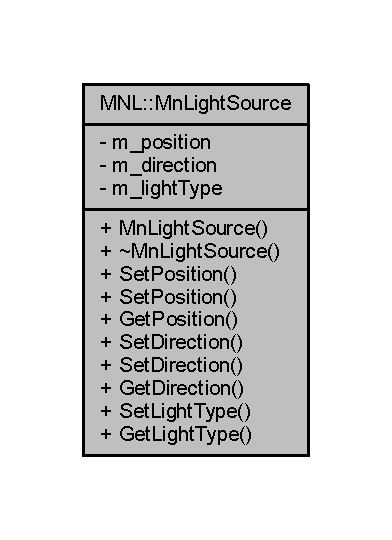
\includegraphics[width=188pt]{class_m_n_l_1_1_mn_light_source__coll__graph}
\end{center}
\end{figure}
\subsection*{Public 멤버 함수}
\begin{DoxyCompactItemize}
\item 
\hyperlink{class_m_n_l_1_1_mn_light_source_a9d944c7ff20f42dfe68bdfe48cc00c84}{Mn\+Light\+Source} ()
\item 
\hyperlink{class_m_n_l_1_1_mn_light_source_a02e32e5231773e772fec046cb4479d48}{$\sim$\+Mn\+Light\+Source} ()
\item 
void \hyperlink{class_m_n_l_1_1_mn_light_source_aa9b9018b18eb6a8adbe7c3af1686ae9a}{Set\+Position} (const Direct\+X\+::\+Simple\+Math\+::\+Vector3 \&position)
\item 
void \hyperlink{class_m_n_l_1_1_mn_light_source_a258cc6ed072e2528e4f6693aa62c2d55}{Set\+Position} (float x, float y, float z)
\item 
const Direct\+X\+::\+Simple\+Math\+::\+Vector3 \& \hyperlink{class_m_n_l_1_1_mn_light_source_ab521d64dec879256da6707bbc4cdb911}{Get\+Position} () const
\item 
void \hyperlink{class_m_n_l_1_1_mn_light_source_a7f9f5ae434cdbd9e34f6994a019ebd95}{Set\+Direction} (const Direct\+X\+::\+Simple\+Math\+::\+Vector3 \&direction)
\item 
void \hyperlink{class_m_n_l_1_1_mn_light_source_adef28f03e9e49b036cd1b8ead7d05498}{Set\+Direction} (float x, float y, float z)
\item 
const Direct\+X\+::\+Simple\+Math\+::\+Vector3 \& \hyperlink{class_m_n_l_1_1_mn_light_source_aa10c767c46c49d278a003cf50cd826d9}{Get\+Direction} () const
\item 
void \hyperlink{class_m_n_l_1_1_mn_light_source_aa0c2232cc2dfa90774a45fd83df082c8}{Set\+Light\+Type} (\hyperlink{namespace_m_n_l_aac0b78de8bb8c872cb617ede813c113d}{M\+N\+\_\+\+L\+I\+G\+H\+T\+\_\+\+T\+Y\+PE} light\+Type)
\item 
const \hyperlink{namespace_m_n_l_aac0b78de8bb8c872cb617ede813c113d}{M\+N\+\_\+\+L\+I\+G\+H\+T\+\_\+\+T\+Y\+PE} \hyperlink{class_m_n_l_1_1_mn_light_source_a9fb139264ff7303e4f3cdb369e198c7a}{Get\+Light\+Type} () const
\end{DoxyCompactItemize}
\subsection*{Private 속성}
\begin{DoxyCompactItemize}
\item 
Direct\+X\+::\+Simple\+Math\+::\+Vector3 \hyperlink{class_m_n_l_1_1_mn_light_source_ad593da80c4bc4a66399facf65d015edf}{m\+\_\+position}
\item 
Direct\+X\+::\+Simple\+Math\+::\+Vector3 \hyperlink{class_m_n_l_1_1_mn_light_source_aaafaae41b829081e37446b58c923e8bf}{m\+\_\+direction}
\item 
\hyperlink{namespace_m_n_l_aac0b78de8bb8c872cb617ede813c113d}{M\+N\+\_\+\+L\+I\+G\+H\+T\+\_\+\+T\+Y\+PE} \hyperlink{class_m_n_l_1_1_mn_light_source_a5d016d5d35ebaef363819340444b41a3}{m\+\_\+light\+Type}
\end{DoxyCompactItemize}


\subsection{상세한 설명}


Mn\+Light\+Source.\+h 파일의 12 번째 라인에서 정의되었습니다.



\subsection{생성자 \& 소멸자 문서화}
\mbox{\Hypertarget{class_m_n_l_1_1_mn_light_source_a9d944c7ff20f42dfe68bdfe48cc00c84}\label{class_m_n_l_1_1_mn_light_source_a9d944c7ff20f42dfe68bdfe48cc00c84}} 
\index{M\+N\+L\+::\+Mn\+Light\+Source@{M\+N\+L\+::\+Mn\+Light\+Source}!Mn\+Light\+Source@{Mn\+Light\+Source}}
\index{Mn\+Light\+Source@{Mn\+Light\+Source}!M\+N\+L\+::\+Mn\+Light\+Source@{M\+N\+L\+::\+Mn\+Light\+Source}}
\subsubsection{\texorpdfstring{Mn\+Light\+Source()}{MnLightSource()}}
{\footnotesize\ttfamily Mn\+Light\+Source\+::\+Mn\+Light\+Source (\begin{DoxyParamCaption}{ }\end{DoxyParamCaption})}



Mn\+Light\+Source.\+cpp 파일의 6 번째 라인에서 정의되었습니다.

\mbox{\Hypertarget{class_m_n_l_1_1_mn_light_source_a02e32e5231773e772fec046cb4479d48}\label{class_m_n_l_1_1_mn_light_source_a02e32e5231773e772fec046cb4479d48}} 
\index{M\+N\+L\+::\+Mn\+Light\+Source@{M\+N\+L\+::\+Mn\+Light\+Source}!````~Mn\+Light\+Source@{$\sim$\+Mn\+Light\+Source}}
\index{````~Mn\+Light\+Source@{$\sim$\+Mn\+Light\+Source}!M\+N\+L\+::\+Mn\+Light\+Source@{M\+N\+L\+::\+Mn\+Light\+Source}}
\subsubsection{\texorpdfstring{$\sim$\+Mn\+Light\+Source()}{~MnLightSource()}}
{\footnotesize\ttfamily Mn\+Light\+Source\+::$\sim$\+Mn\+Light\+Source (\begin{DoxyParamCaption}{ }\end{DoxyParamCaption})}



Mn\+Light\+Source.\+cpp 파일의 14 번째 라인에서 정의되었습니다.



\subsection{멤버 함수 문서화}
\mbox{\Hypertarget{class_m_n_l_1_1_mn_light_source_aa10c767c46c49d278a003cf50cd826d9}\label{class_m_n_l_1_1_mn_light_source_aa10c767c46c49d278a003cf50cd826d9}} 
\index{M\+N\+L\+::\+Mn\+Light\+Source@{M\+N\+L\+::\+Mn\+Light\+Source}!Get\+Direction@{Get\+Direction}}
\index{Get\+Direction@{Get\+Direction}!M\+N\+L\+::\+Mn\+Light\+Source@{M\+N\+L\+::\+Mn\+Light\+Source}}
\subsubsection{\texorpdfstring{Get\+Direction()}{GetDirection()}}
{\footnotesize\ttfamily const Direct\+X\+::\+Simple\+Math\+::\+Vector3 \& Mn\+Light\+Source\+::\+Get\+Direction (\begin{DoxyParamCaption}{ }\end{DoxyParamCaption}) const}



Mn\+Light\+Source.\+cpp 파일의 44 번째 라인에서 정의되었습니다.

\mbox{\Hypertarget{class_m_n_l_1_1_mn_light_source_a9fb139264ff7303e4f3cdb369e198c7a}\label{class_m_n_l_1_1_mn_light_source_a9fb139264ff7303e4f3cdb369e198c7a}} 
\index{M\+N\+L\+::\+Mn\+Light\+Source@{M\+N\+L\+::\+Mn\+Light\+Source}!Get\+Light\+Type@{Get\+Light\+Type}}
\index{Get\+Light\+Type@{Get\+Light\+Type}!M\+N\+L\+::\+Mn\+Light\+Source@{M\+N\+L\+::\+Mn\+Light\+Source}}
\subsubsection{\texorpdfstring{Get\+Light\+Type()}{GetLightType()}}
{\footnotesize\ttfamily const \hyperlink{namespace_m_n_l_aac0b78de8bb8c872cb617ede813c113d}{M\+N\+\_\+\+L\+I\+G\+H\+T\+\_\+\+T\+Y\+PE} Mn\+Light\+Source\+::\+Get\+Light\+Type (\begin{DoxyParamCaption}{ }\end{DoxyParamCaption}) const}



Mn\+Light\+Source.\+cpp 파일의 52 번째 라인에서 정의되었습니다.

\mbox{\Hypertarget{class_m_n_l_1_1_mn_light_source_ab521d64dec879256da6707bbc4cdb911}\label{class_m_n_l_1_1_mn_light_source_ab521d64dec879256da6707bbc4cdb911}} 
\index{M\+N\+L\+::\+Mn\+Light\+Source@{M\+N\+L\+::\+Mn\+Light\+Source}!Get\+Position@{Get\+Position}}
\index{Get\+Position@{Get\+Position}!M\+N\+L\+::\+Mn\+Light\+Source@{M\+N\+L\+::\+Mn\+Light\+Source}}
\subsubsection{\texorpdfstring{Get\+Position()}{GetPosition()}}
{\footnotesize\ttfamily const Direct\+X\+::\+Simple\+Math\+::\+Vector3 \& Mn\+Light\+Source\+::\+Get\+Position (\begin{DoxyParamCaption}{ }\end{DoxyParamCaption}) const}



Mn\+Light\+Source.\+cpp 파일의 29 번째 라인에서 정의되었습니다.

\mbox{\Hypertarget{class_m_n_l_1_1_mn_light_source_a7f9f5ae434cdbd9e34f6994a019ebd95}\label{class_m_n_l_1_1_mn_light_source_a7f9f5ae434cdbd9e34f6994a019ebd95}} 
\index{M\+N\+L\+::\+Mn\+Light\+Source@{M\+N\+L\+::\+Mn\+Light\+Source}!Set\+Direction@{Set\+Direction}}
\index{Set\+Direction@{Set\+Direction}!M\+N\+L\+::\+Mn\+Light\+Source@{M\+N\+L\+::\+Mn\+Light\+Source}}
\subsubsection{\texorpdfstring{Set\+Direction()}{SetDirection()}\hspace{0.1cm}{\footnotesize\ttfamily [1/2]}}
{\footnotesize\ttfamily void Mn\+Light\+Source\+::\+Set\+Direction (\begin{DoxyParamCaption}\item[{const Direct\+X\+::\+Simple\+Math\+::\+Vector3 \&}]{direction }\end{DoxyParamCaption})}



Mn\+Light\+Source.\+cpp 파일의 34 번째 라인에서 정의되었습니다.

\mbox{\Hypertarget{class_m_n_l_1_1_mn_light_source_adef28f03e9e49b036cd1b8ead7d05498}\label{class_m_n_l_1_1_mn_light_source_adef28f03e9e49b036cd1b8ead7d05498}} 
\index{M\+N\+L\+::\+Mn\+Light\+Source@{M\+N\+L\+::\+Mn\+Light\+Source}!Set\+Direction@{Set\+Direction}}
\index{Set\+Direction@{Set\+Direction}!M\+N\+L\+::\+Mn\+Light\+Source@{M\+N\+L\+::\+Mn\+Light\+Source}}
\subsubsection{\texorpdfstring{Set\+Direction()}{SetDirection()}\hspace{0.1cm}{\footnotesize\ttfamily [2/2]}}
{\footnotesize\ttfamily void Mn\+Light\+Source\+::\+Set\+Direction (\begin{DoxyParamCaption}\item[{float}]{x,  }\item[{float}]{y,  }\item[{float}]{z }\end{DoxyParamCaption})}



Mn\+Light\+Source.\+cpp 파일의 38 번째 라인에서 정의되었습니다.

\mbox{\Hypertarget{class_m_n_l_1_1_mn_light_source_aa0c2232cc2dfa90774a45fd83df082c8}\label{class_m_n_l_1_1_mn_light_source_aa0c2232cc2dfa90774a45fd83df082c8}} 
\index{M\+N\+L\+::\+Mn\+Light\+Source@{M\+N\+L\+::\+Mn\+Light\+Source}!Set\+Light\+Type@{Set\+Light\+Type}}
\index{Set\+Light\+Type@{Set\+Light\+Type}!M\+N\+L\+::\+Mn\+Light\+Source@{M\+N\+L\+::\+Mn\+Light\+Source}}
\subsubsection{\texorpdfstring{Set\+Light\+Type()}{SetLightType()}}
{\footnotesize\ttfamily void Mn\+Light\+Source\+::\+Set\+Light\+Type (\begin{DoxyParamCaption}\item[{\hyperlink{namespace_m_n_l_aac0b78de8bb8c872cb617ede813c113d}{M\+N\+\_\+\+L\+I\+G\+H\+T\+\_\+\+T\+Y\+PE}}]{light\+Type }\end{DoxyParamCaption})}



Mn\+Light\+Source.\+cpp 파일의 48 번째 라인에서 정의되었습니다.

\mbox{\Hypertarget{class_m_n_l_1_1_mn_light_source_aa9b9018b18eb6a8adbe7c3af1686ae9a}\label{class_m_n_l_1_1_mn_light_source_aa9b9018b18eb6a8adbe7c3af1686ae9a}} 
\index{M\+N\+L\+::\+Mn\+Light\+Source@{M\+N\+L\+::\+Mn\+Light\+Source}!Set\+Position@{Set\+Position}}
\index{Set\+Position@{Set\+Position}!M\+N\+L\+::\+Mn\+Light\+Source@{M\+N\+L\+::\+Mn\+Light\+Source}}
\subsubsection{\texorpdfstring{Set\+Position()}{SetPosition()}\hspace{0.1cm}{\footnotesize\ttfamily [1/2]}}
{\footnotesize\ttfamily void Mn\+Light\+Source\+::\+Set\+Position (\begin{DoxyParamCaption}\item[{const Direct\+X\+::\+Simple\+Math\+::\+Vector3 \&}]{position }\end{DoxyParamCaption})}



Mn\+Light\+Source.\+cpp 파일의 19 번째 라인에서 정의되었습니다.

\mbox{\Hypertarget{class_m_n_l_1_1_mn_light_source_a258cc6ed072e2528e4f6693aa62c2d55}\label{class_m_n_l_1_1_mn_light_source_a258cc6ed072e2528e4f6693aa62c2d55}} 
\index{M\+N\+L\+::\+Mn\+Light\+Source@{M\+N\+L\+::\+Mn\+Light\+Source}!Set\+Position@{Set\+Position}}
\index{Set\+Position@{Set\+Position}!M\+N\+L\+::\+Mn\+Light\+Source@{M\+N\+L\+::\+Mn\+Light\+Source}}
\subsubsection{\texorpdfstring{Set\+Position()}{SetPosition()}\hspace{0.1cm}{\footnotesize\ttfamily [2/2]}}
{\footnotesize\ttfamily void Mn\+Light\+Source\+::\+Set\+Position (\begin{DoxyParamCaption}\item[{float}]{x,  }\item[{float}]{y,  }\item[{float}]{z }\end{DoxyParamCaption})}



Mn\+Light\+Source.\+cpp 파일의 23 번째 라인에서 정의되었습니다.



\subsection{멤버 데이터 문서화}
\mbox{\Hypertarget{class_m_n_l_1_1_mn_light_source_aaafaae41b829081e37446b58c923e8bf}\label{class_m_n_l_1_1_mn_light_source_aaafaae41b829081e37446b58c923e8bf}} 
\index{M\+N\+L\+::\+Mn\+Light\+Source@{M\+N\+L\+::\+Mn\+Light\+Source}!m\+\_\+direction@{m\+\_\+direction}}
\index{m\+\_\+direction@{m\+\_\+direction}!M\+N\+L\+::\+Mn\+Light\+Source@{M\+N\+L\+::\+Mn\+Light\+Source}}
\subsubsection{\texorpdfstring{m\+\_\+direction}{m\_direction}}
{\footnotesize\ttfamily Direct\+X\+::\+Simple\+Math\+::\+Vector3 M\+N\+L\+::\+Mn\+Light\+Source\+::m\+\_\+direction\hspace{0.3cm}{\ttfamily [private]}}



Mn\+Light\+Source.\+h 파일의 31 번째 라인에서 정의되었습니다.

\mbox{\Hypertarget{class_m_n_l_1_1_mn_light_source_a5d016d5d35ebaef363819340444b41a3}\label{class_m_n_l_1_1_mn_light_source_a5d016d5d35ebaef363819340444b41a3}} 
\index{M\+N\+L\+::\+Mn\+Light\+Source@{M\+N\+L\+::\+Mn\+Light\+Source}!m\+\_\+light\+Type@{m\+\_\+light\+Type}}
\index{m\+\_\+light\+Type@{m\+\_\+light\+Type}!M\+N\+L\+::\+Mn\+Light\+Source@{M\+N\+L\+::\+Mn\+Light\+Source}}
\subsubsection{\texorpdfstring{m\+\_\+light\+Type}{m\_lightType}}
{\footnotesize\ttfamily \hyperlink{namespace_m_n_l_aac0b78de8bb8c872cb617ede813c113d}{M\+N\+\_\+\+L\+I\+G\+H\+T\+\_\+\+T\+Y\+PE} M\+N\+L\+::\+Mn\+Light\+Source\+::m\+\_\+light\+Type\hspace{0.3cm}{\ttfamily [private]}}



Mn\+Light\+Source.\+h 파일의 32 번째 라인에서 정의되었습니다.

\mbox{\Hypertarget{class_m_n_l_1_1_mn_light_source_ad593da80c4bc4a66399facf65d015edf}\label{class_m_n_l_1_1_mn_light_source_ad593da80c4bc4a66399facf65d015edf}} 
\index{M\+N\+L\+::\+Mn\+Light\+Source@{M\+N\+L\+::\+Mn\+Light\+Source}!m\+\_\+position@{m\+\_\+position}}
\index{m\+\_\+position@{m\+\_\+position}!M\+N\+L\+::\+Mn\+Light\+Source@{M\+N\+L\+::\+Mn\+Light\+Source}}
\subsubsection{\texorpdfstring{m\+\_\+position}{m\_position}}
{\footnotesize\ttfamily Direct\+X\+::\+Simple\+Math\+::\+Vector3 M\+N\+L\+::\+Mn\+Light\+Source\+::m\+\_\+position\hspace{0.3cm}{\ttfamily [private]}}



Mn\+Light\+Source.\+h 파일의 30 번째 라인에서 정의되었습니다.



이 클래스에 대한 문서화 페이지는 다음의 파일들로부터 생성되었습니다.\+:\begin{DoxyCompactItemize}
\item 
Render/\hyperlink{_mn_light_source_8h}{Mn\+Light\+Source.\+h}\item 
Render/\hyperlink{_mn_light_source_8cpp}{Mn\+Light\+Source.\+cpp}\end{DoxyCompactItemize}

\hypertarget{class_m_n_l_1_1_mn_material}{}\section{M\+NL\+:\+:Mn\+Material 클래스 참조}
\label{class_m_n_l_1_1_mn_material}\index{M\+N\+L\+::\+Mn\+Material@{M\+N\+L\+::\+Mn\+Material}}


{\ttfamily \#include $<$Mn\+Material.\+h$>$}



M\+NL\+:\+:Mn\+Material에 대한 협력 다이어그램\+:\nopagebreak
\begin{figure}[H]
\begin{center}
\leavevmode
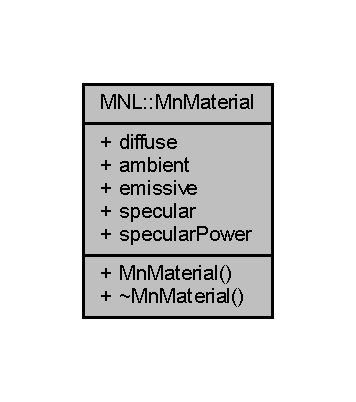
\includegraphics[width=171pt]{class_m_n_l_1_1_mn_material__coll__graph}
\end{center}
\end{figure}
\subsection*{Public 멤버 함수}
\begin{DoxyCompactItemize}
\item 
\hyperlink{class_m_n_l_1_1_mn_material_aad9a010b9ae350c5c1f33f81bdc2bebb}{Mn\+Material} ()
\item 
\hyperlink{class_m_n_l_1_1_mn_material_a5eb1c2ba8f8deac5d1cce68e00b7c4f6}{$\sim$\+Mn\+Material} ()
\end{DoxyCompactItemize}
\subsection*{Public 속성}
\begin{DoxyCompactItemize}
\item 
Direct\+X\+::\+Simple\+Math\+::\+Vector4 \hyperlink{class_m_n_l_1_1_mn_material_a0286b31f8f107f8c538f0db9a18acaa2}{diffuse}
\item 
Direct\+X\+::\+Simple\+Math\+::\+Vector4 \hyperlink{class_m_n_l_1_1_mn_material_aa6897e5662f3dbac8f72e96ef722ac0d}{ambient}
\item 
Direct\+X\+::\+Simple\+Math\+::\+Vector4 \hyperlink{class_m_n_l_1_1_mn_material_a58bf008b04d0245f6470da8ca3d4d735}{emissive}
\item 
Direct\+X\+::\+Simple\+Math\+::\+Vector4 \hyperlink{class_m_n_l_1_1_mn_material_a7f083df1bc6578e41917bd4a237448bf}{specular}
\item 
float \hyperlink{class_m_n_l_1_1_mn_material_abfcc4a9b518663738879256b440e432a}{specular\+Power}
\end{DoxyCompactItemize}


\subsection{상세한 설명}


Mn\+Material.\+h 파일의 10 번째 라인에서 정의되었습니다.



\subsection{생성자 \& 소멸자 문서화}
\mbox{\Hypertarget{class_m_n_l_1_1_mn_material_aad9a010b9ae350c5c1f33f81bdc2bebb}\label{class_m_n_l_1_1_mn_material_aad9a010b9ae350c5c1f33f81bdc2bebb}} 
\index{M\+N\+L\+::\+Mn\+Material@{M\+N\+L\+::\+Mn\+Material}!Mn\+Material@{Mn\+Material}}
\index{Mn\+Material@{Mn\+Material}!M\+N\+L\+::\+Mn\+Material@{M\+N\+L\+::\+Mn\+Material}}
\subsubsection{\texorpdfstring{Mn\+Material()}{MnMaterial()}}
{\footnotesize\ttfamily Mn\+Material\+::\+Mn\+Material (\begin{DoxyParamCaption}{ }\end{DoxyParamCaption})}



Mn\+Material.\+cpp 파일의 5 번째 라인에서 정의되었습니다.

\mbox{\Hypertarget{class_m_n_l_1_1_mn_material_a5eb1c2ba8f8deac5d1cce68e00b7c4f6}\label{class_m_n_l_1_1_mn_material_a5eb1c2ba8f8deac5d1cce68e00b7c4f6}} 
\index{M\+N\+L\+::\+Mn\+Material@{M\+N\+L\+::\+Mn\+Material}!````~Mn\+Material@{$\sim$\+Mn\+Material}}
\index{````~Mn\+Material@{$\sim$\+Mn\+Material}!M\+N\+L\+::\+Mn\+Material@{M\+N\+L\+::\+Mn\+Material}}
\subsubsection{\texorpdfstring{$\sim$\+Mn\+Material()}{~MnMaterial()}}
{\footnotesize\ttfamily Mn\+Material\+::$\sim$\+Mn\+Material (\begin{DoxyParamCaption}{ }\end{DoxyParamCaption})}



Mn\+Material.\+cpp 파일의 14 번째 라인에서 정의되었습니다.



\subsection{멤버 데이터 문서화}
\mbox{\Hypertarget{class_m_n_l_1_1_mn_material_aa6897e5662f3dbac8f72e96ef722ac0d}\label{class_m_n_l_1_1_mn_material_aa6897e5662f3dbac8f72e96ef722ac0d}} 
\index{M\+N\+L\+::\+Mn\+Material@{M\+N\+L\+::\+Mn\+Material}!ambient@{ambient}}
\index{ambient@{ambient}!M\+N\+L\+::\+Mn\+Material@{M\+N\+L\+::\+Mn\+Material}}
\subsubsection{\texorpdfstring{ambient}{ambient}}
{\footnotesize\ttfamily Direct\+X\+::\+Simple\+Math\+::\+Vector4 M\+N\+L\+::\+Mn\+Material\+::ambient}



Mn\+Material.\+h 파일의 17 번째 라인에서 정의되었습니다.

\mbox{\Hypertarget{class_m_n_l_1_1_mn_material_a0286b31f8f107f8c538f0db9a18acaa2}\label{class_m_n_l_1_1_mn_material_a0286b31f8f107f8c538f0db9a18acaa2}} 
\index{M\+N\+L\+::\+Mn\+Material@{M\+N\+L\+::\+Mn\+Material}!diffuse@{diffuse}}
\index{diffuse@{diffuse}!M\+N\+L\+::\+Mn\+Material@{M\+N\+L\+::\+Mn\+Material}}
\subsubsection{\texorpdfstring{diffuse}{diffuse}}
{\footnotesize\ttfamily Direct\+X\+::\+Simple\+Math\+::\+Vector4 M\+N\+L\+::\+Mn\+Material\+::diffuse}



Mn\+Material.\+h 파일의 16 번째 라인에서 정의되었습니다.

\mbox{\Hypertarget{class_m_n_l_1_1_mn_material_a58bf008b04d0245f6470da8ca3d4d735}\label{class_m_n_l_1_1_mn_material_a58bf008b04d0245f6470da8ca3d4d735}} 
\index{M\+N\+L\+::\+Mn\+Material@{M\+N\+L\+::\+Mn\+Material}!emissive@{emissive}}
\index{emissive@{emissive}!M\+N\+L\+::\+Mn\+Material@{M\+N\+L\+::\+Mn\+Material}}
\subsubsection{\texorpdfstring{emissive}{emissive}}
{\footnotesize\ttfamily Direct\+X\+::\+Simple\+Math\+::\+Vector4 M\+N\+L\+::\+Mn\+Material\+::emissive}



Mn\+Material.\+h 파일의 18 번째 라인에서 정의되었습니다.

\mbox{\Hypertarget{class_m_n_l_1_1_mn_material_a7f083df1bc6578e41917bd4a237448bf}\label{class_m_n_l_1_1_mn_material_a7f083df1bc6578e41917bd4a237448bf}} 
\index{M\+N\+L\+::\+Mn\+Material@{M\+N\+L\+::\+Mn\+Material}!specular@{specular}}
\index{specular@{specular}!M\+N\+L\+::\+Mn\+Material@{M\+N\+L\+::\+Mn\+Material}}
\subsubsection{\texorpdfstring{specular}{specular}}
{\footnotesize\ttfamily Direct\+X\+::\+Simple\+Math\+::\+Vector4 M\+N\+L\+::\+Mn\+Material\+::specular}



Mn\+Material.\+h 파일의 19 번째 라인에서 정의되었습니다.

\mbox{\Hypertarget{class_m_n_l_1_1_mn_material_abfcc4a9b518663738879256b440e432a}\label{class_m_n_l_1_1_mn_material_abfcc4a9b518663738879256b440e432a}} 
\index{M\+N\+L\+::\+Mn\+Material@{M\+N\+L\+::\+Mn\+Material}!specular\+Power@{specular\+Power}}
\index{specular\+Power@{specular\+Power}!M\+N\+L\+::\+Mn\+Material@{M\+N\+L\+::\+Mn\+Material}}
\subsubsection{\texorpdfstring{specular\+Power}{specularPower}}
{\footnotesize\ttfamily float M\+N\+L\+::\+Mn\+Material\+::specular\+Power}



Mn\+Material.\+h 파일의 20 번째 라인에서 정의되었습니다.



이 클래스에 대한 문서화 페이지는 다음의 파일들로부터 생성되었습니다.\+:\begin{DoxyCompactItemize}
\item 
Render/\hyperlink{_mn_material_8h}{Mn\+Material.\+h}\item 
Render/\hyperlink{_mn_material_8cpp}{Mn\+Material.\+cpp}\end{DoxyCompactItemize}

\hypertarget{class_m_n_l_1_1_mn_matrix_palette}{}\section{M\+NL\+:\+:Mn\+Matrix\+Palette 클래스 참조}
\label{class_m_n_l_1_1_mn_matrix_palette}\index{M\+N\+L\+::\+Mn\+Matrix\+Palette@{M\+N\+L\+::\+Mn\+Matrix\+Palette}}


{\ttfamily \#include $<$Mn\+Matrix\+Palette.\+h$>$}



M\+NL\+:\+:Mn\+Matrix\+Palette에 대한 협력 다이어그램\+:\nopagebreak
\begin{figure}[H]
\begin{center}
\leavevmode
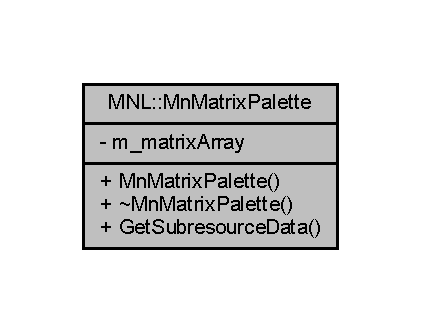
\includegraphics[width=202pt]{class_m_n_l_1_1_mn_matrix_palette__coll__graph}
\end{center}
\end{figure}
\subsection*{Public 멤버 함수}
\begin{DoxyCompactItemize}
\item 
\hyperlink{class_m_n_l_1_1_mn_matrix_palette_a5952293984870cc9ce39a105370e7012}{Mn\+Matrix\+Palette} ()
\item 
\hyperlink{class_m_n_l_1_1_mn_matrix_palette_a3492e52b69c245bc74f5af5e9913e9c4}{$\sim$\+Mn\+Matrix\+Palette} ()
\item 
D3\+D11\+\_\+\+S\+U\+B\+R\+E\+S\+O\+U\+R\+C\+E\+\_\+\+D\+A\+TA \hyperlink{class_m_n_l_1_1_mn_matrix_palette_ad7ffb57f4795ced63d95eb0fef6220aa}{Get\+Subresource\+Data} () const
\end{DoxyCompactItemize}
\subsection*{Private 속성}
\begin{DoxyCompactItemize}
\item 
std\+::vector$<$ Direct\+X\+::\+Simple\+Math\+::\+Matrix $>$ \hyperlink{class_m_n_l_1_1_mn_matrix_palette_a75048f096e7fe205df32f0603f96a50a}{m\+\_\+matrix\+Array}
\end{DoxyCompactItemize}


\subsection{상세한 설명}


Mn\+Matrix\+Palette.\+h 파일의 10 번째 라인에서 정의되었습니다.



\subsection{생성자 \& 소멸자 문서화}
\mbox{\Hypertarget{class_m_n_l_1_1_mn_matrix_palette_a5952293984870cc9ce39a105370e7012}\label{class_m_n_l_1_1_mn_matrix_palette_a5952293984870cc9ce39a105370e7012}} 
\index{M\+N\+L\+::\+Mn\+Matrix\+Palette@{M\+N\+L\+::\+Mn\+Matrix\+Palette}!Mn\+Matrix\+Palette@{Mn\+Matrix\+Palette}}
\index{Mn\+Matrix\+Palette@{Mn\+Matrix\+Palette}!M\+N\+L\+::\+Mn\+Matrix\+Palette@{M\+N\+L\+::\+Mn\+Matrix\+Palette}}
\subsubsection{\texorpdfstring{Mn\+Matrix\+Palette()}{MnMatrixPalette()}}
{\footnotesize\ttfamily Mn\+Matrix\+Palette\+::\+Mn\+Matrix\+Palette (\begin{DoxyParamCaption}{ }\end{DoxyParamCaption})}



Mn\+Matrix\+Palette.\+cpp 파일의 5 번째 라인에서 정의되었습니다.

\mbox{\Hypertarget{class_m_n_l_1_1_mn_matrix_palette_a3492e52b69c245bc74f5af5e9913e9c4}\label{class_m_n_l_1_1_mn_matrix_palette_a3492e52b69c245bc74f5af5e9913e9c4}} 
\index{M\+N\+L\+::\+Mn\+Matrix\+Palette@{M\+N\+L\+::\+Mn\+Matrix\+Palette}!````~Mn\+Matrix\+Palette@{$\sim$\+Mn\+Matrix\+Palette}}
\index{````~Mn\+Matrix\+Palette@{$\sim$\+Mn\+Matrix\+Palette}!M\+N\+L\+::\+Mn\+Matrix\+Palette@{M\+N\+L\+::\+Mn\+Matrix\+Palette}}
\subsubsection{\texorpdfstring{$\sim$\+Mn\+Matrix\+Palette()}{~MnMatrixPalette()}}
{\footnotesize\ttfamily Mn\+Matrix\+Palette\+::$\sim$\+Mn\+Matrix\+Palette (\begin{DoxyParamCaption}{ }\end{DoxyParamCaption})}



Mn\+Matrix\+Palette.\+cpp 파일의 9 번째 라인에서 정의되었습니다.



\subsection{멤버 함수 문서화}
\mbox{\Hypertarget{class_m_n_l_1_1_mn_matrix_palette_ad7ffb57f4795ced63d95eb0fef6220aa}\label{class_m_n_l_1_1_mn_matrix_palette_ad7ffb57f4795ced63d95eb0fef6220aa}} 
\index{M\+N\+L\+::\+Mn\+Matrix\+Palette@{M\+N\+L\+::\+Mn\+Matrix\+Palette}!Get\+Subresource\+Data@{Get\+Subresource\+Data}}
\index{Get\+Subresource\+Data@{Get\+Subresource\+Data}!M\+N\+L\+::\+Mn\+Matrix\+Palette@{M\+N\+L\+::\+Mn\+Matrix\+Palette}}
\subsubsection{\texorpdfstring{Get\+Subresource\+Data()}{GetSubresourceData()}}
{\footnotesize\ttfamily D3\+D11\+\_\+\+S\+U\+B\+R\+E\+S\+O\+U\+R\+C\+E\+\_\+\+D\+A\+TA Mn\+Matrix\+Palette\+::\+Get\+Subresource\+Data (\begin{DoxyParamCaption}{ }\end{DoxyParamCaption}) const}



Mn\+Matrix\+Palette.\+cpp 파일의 13 번째 라인에서 정의되었습니다.



\subsection{멤버 데이터 문서화}
\mbox{\Hypertarget{class_m_n_l_1_1_mn_matrix_palette_a75048f096e7fe205df32f0603f96a50a}\label{class_m_n_l_1_1_mn_matrix_palette_a75048f096e7fe205df32f0603f96a50a}} 
\index{M\+N\+L\+::\+Mn\+Matrix\+Palette@{M\+N\+L\+::\+Mn\+Matrix\+Palette}!m\+\_\+matrix\+Array@{m\+\_\+matrix\+Array}}
\index{m\+\_\+matrix\+Array@{m\+\_\+matrix\+Array}!M\+N\+L\+::\+Mn\+Matrix\+Palette@{M\+N\+L\+::\+Mn\+Matrix\+Palette}}
\subsubsection{\texorpdfstring{m\+\_\+matrix\+Array}{m\_matrixArray}}
{\footnotesize\ttfamily std\+::vector$<$Direct\+X\+::\+Simple\+Math\+::\+Matrix$>$ M\+N\+L\+::\+Mn\+Matrix\+Palette\+::m\+\_\+matrix\+Array\hspace{0.3cm}{\ttfamily [private]}}



Mn\+Matrix\+Palette.\+h 파일의 18 번째 라인에서 정의되었습니다.



이 클래스에 대한 문서화 페이지는 다음의 파일들로부터 생성되었습니다.\+:\begin{DoxyCompactItemize}
\item 
Render/\hyperlink{_mn_matrix_palette_8h}{Mn\+Matrix\+Palette.\+h}\item 
Render/\hyperlink{_mn_matrix_palette_8cpp}{Mn\+Matrix\+Palette.\+cpp}\end{DoxyCompactItemize}

\hypertarget{class_m_n_l_1_1_mn_mesh}{}\section{M\+NL\+:\+:Mn\+Mesh 클래스 참조}
\label{class_m_n_l_1_1_mn_mesh}\index{M\+N\+L\+::\+Mn\+Mesh@{M\+N\+L\+::\+Mn\+Mesh}}


{\ttfamily \#include $<$Mn\+Mesh.\+h$>$}



M\+NL\+:\+:Mn\+Mesh에 대한 상속 다이어그램 \+: \nopagebreak
\begin{figure}[H]
\begin{center}
\leavevmode
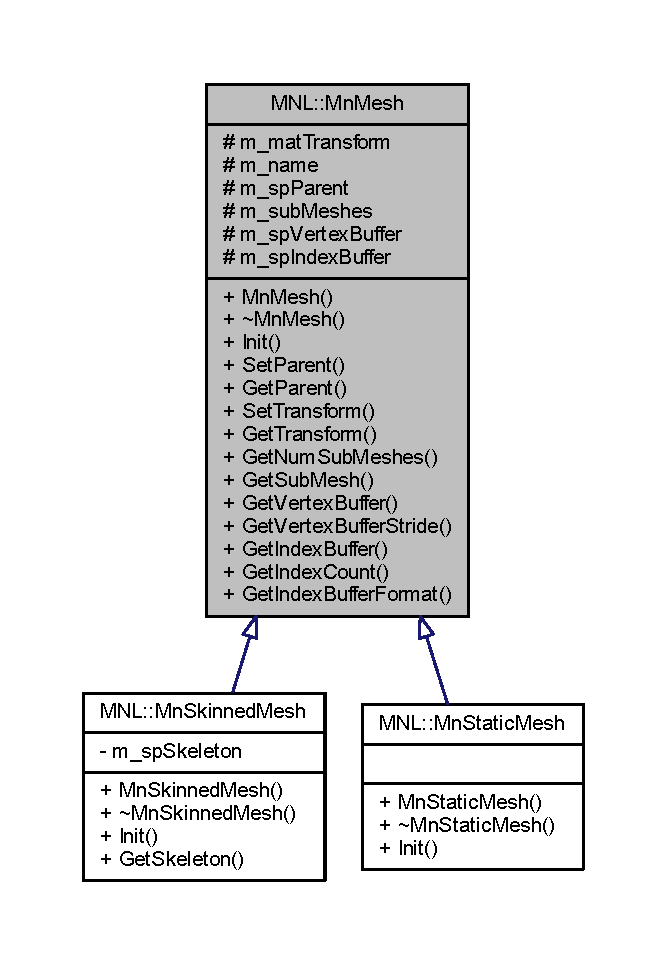
\includegraphics[width=320pt]{class_m_n_l_1_1_mn_mesh__inherit__graph}
\end{center}
\end{figure}


M\+NL\+:\+:Mn\+Mesh에 대한 협력 다이어그램\+:\nopagebreak
\begin{figure}[H]
\begin{center}
\leavevmode
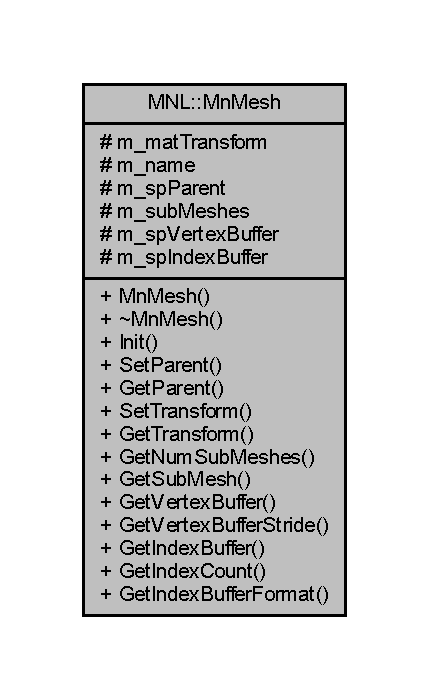
\includegraphics[width=206pt]{class_m_n_l_1_1_mn_mesh__coll__graph}
\end{center}
\end{figure}
\subsection*{Public 멤버 함수}
\begin{DoxyCompactItemize}
\item 
\hyperlink{class_m_n_l_1_1_mn_mesh_a5a2ad03a6baa88d7563df3cc17e36b12}{Mn\+Mesh} ()
\item 
\hyperlink{class_m_n_l_1_1_mn_mesh_a35cdd9cc547aa3e32ba67f09b74bac01}{$\sim$\+Mn\+Mesh} ()
\item 
virtual H\+R\+E\+S\+U\+LT \hyperlink{class_m_n_l_1_1_mn_mesh_a694b6dfe0ae3ed0f97bcf055525b8659}{Init} (const \hyperlink{namespace_m_n_l_a1eec210db8f309a4a9ac0d9658784c31}{C\+P\+D3\+D\+Device} \&cp\+Device, const std\+::shared\+\_\+ptr$<$ \hyperlink{class_m_n_l_1_1_mn_mesh_data}{Mn\+Mesh\+Data} $>$ sp\+Mesh\+Data)
\item 
void \hyperlink{class_m_n_l_1_1_mn_mesh_a05cb7889b4f8ce6ed32334082ea9ac4c}{Set\+Parent} (const std\+::shared\+\_\+ptr$<$ \hyperlink{class_m_n_l_1_1_mn_mesh}{Mn\+Mesh} $>$ \&sp\+Mesh)
\item 
std\+::shared\+\_\+ptr$<$ \hyperlink{class_m_n_l_1_1_mn_mesh}{Mn\+Mesh} $>$ \hyperlink{class_m_n_l_1_1_mn_mesh_a04364fc880cefe0dfbf99c4196d25cfd}{Get\+Parent} () const
\item 
void \hyperlink{class_m_n_l_1_1_mn_mesh_a47ce5880e4d73b11887c83921824f43d}{Set\+Transform} (const Direct\+X\+::\+Simple\+Math\+::\+Matrix \&mat\+Transform)
\item 
const Direct\+X\+::\+Simple\+Math\+::\+Matrix \& \hyperlink{class_m_n_l_1_1_mn_mesh_a6e1178196c41f872f432a65a02a786e5}{Get\+Transform} () const
\item 
U\+I\+NT \hyperlink{class_m_n_l_1_1_mn_mesh_aee1f713bc53686879397376a064cdf2b}{Get\+Num\+Sub\+Meshes} () const
\item 
const \hyperlink{struct_m_n_l_1_1_mn_sub_mesh}{Mn\+Sub\+Mesh} \& \hyperlink{class_m_n_l_1_1_mn_mesh_ab765c79f606507de6d1be69f51ec2502}{Get\+Sub\+Mesh} (U\+I\+NT index) const
\item 
const \hyperlink{namespace_m_n_l_aab9c90a8c27ac6410a9cc7cd89efeef1}{C\+P\+D3\+D\+Buffer} \hyperlink{class_m_n_l_1_1_mn_mesh_a3c8f3380c7ea8a5927a61e667400e9a8}{Get\+Vertex\+Buffer} () const
\item 
U\+I\+NT \hyperlink{class_m_n_l_1_1_mn_mesh_aa8706a7d5ca39d4666867c24d5a3be5a}{Get\+Vertex\+Buffer\+Stride} () const
\item 
const \hyperlink{namespace_m_n_l_aab9c90a8c27ac6410a9cc7cd89efeef1}{C\+P\+D3\+D\+Buffer} \hyperlink{class_m_n_l_1_1_mn_mesh_a2e8ea6dbb3625a0700e092a7293bd6e7}{Get\+Index\+Buffer} () const
\item 
U\+I\+NT \hyperlink{class_m_n_l_1_1_mn_mesh_aba80f0a52329029f340414c71cdfe8c8}{Get\+Index\+Count} () const
\item 
D\+X\+G\+I\+\_\+\+F\+O\+R\+M\+AT \hyperlink{class_m_n_l_1_1_mn_mesh_a48b3d12651791c91095a883aef2e577d}{Get\+Index\+Buffer\+Format} () const
\end{DoxyCompactItemize}
\subsection*{Protected 속성}
\begin{DoxyCompactItemize}
\item 
Direct\+X\+::\+Simple\+Math\+::\+Matrix \hyperlink{class_m_n_l_1_1_mn_mesh_a3617de4ff06fb44e929375c976749e39}{m\+\_\+mat\+Transform}
\item 
std\+::string \hyperlink{class_m_n_l_1_1_mn_mesh_a571897045eb370a1f780cf13e9c34113}{m\+\_\+name}
\item 
std\+::shared\+\_\+ptr$<$ \hyperlink{class_m_n_l_1_1_mn_mesh}{Mn\+Mesh} $>$ \hyperlink{class_m_n_l_1_1_mn_mesh_a5fcd00e08db33a48849fb837a4ac971f}{m\+\_\+sp\+Parent}
\item 
std\+::vector$<$ \hyperlink{struct_m_n_l_1_1_mn_sub_mesh}{Mn\+Sub\+Mesh} $>$ \hyperlink{class_m_n_l_1_1_mn_mesh_a1319f6800c28153c09fba2eb1843a41d}{m\+\_\+sub\+Meshes}
\item 
std\+::shared\+\_\+ptr$<$ \hyperlink{class_m_n_l_1_1_mn_vertex_buffer}{Mn\+Vertex\+Buffer} $>$ \hyperlink{class_m_n_l_1_1_mn_mesh_aff6e55968332581a0848069303689fa4}{m\+\_\+sp\+Vertex\+Buffer}
\item 
std\+::shared\+\_\+ptr$<$ \hyperlink{class_m_n_l_1_1_mn_index_buffer}{Mn\+Index\+Buffer} $>$ \hyperlink{class_m_n_l_1_1_mn_mesh_a03f3e7ccea4728ab9f6846eca2794dd8}{m\+\_\+sp\+Index\+Buffer}
\end{DoxyCompactItemize}


\subsection{상세한 설명}


Mn\+Mesh.\+h 파일의 17 번째 라인에서 정의되었습니다.



\subsection{생성자 \& 소멸자 문서화}
\mbox{\Hypertarget{class_m_n_l_1_1_mn_mesh_a5a2ad03a6baa88d7563df3cc17e36b12}\label{class_m_n_l_1_1_mn_mesh_a5a2ad03a6baa88d7563df3cc17e36b12}} 
\index{M\+N\+L\+::\+Mn\+Mesh@{M\+N\+L\+::\+Mn\+Mesh}!Mn\+Mesh@{Mn\+Mesh}}
\index{Mn\+Mesh@{Mn\+Mesh}!M\+N\+L\+::\+Mn\+Mesh@{M\+N\+L\+::\+Mn\+Mesh}}
\subsubsection{\texorpdfstring{Mn\+Mesh()}{MnMesh()}}
{\footnotesize\ttfamily Mn\+Mesh\+::\+Mn\+Mesh (\begin{DoxyParamCaption}{ }\end{DoxyParamCaption})}



Mn\+Mesh.\+cpp 파일의 6 번째 라인에서 정의되었습니다.

\mbox{\Hypertarget{class_m_n_l_1_1_mn_mesh_a35cdd9cc547aa3e32ba67f09b74bac01}\label{class_m_n_l_1_1_mn_mesh_a35cdd9cc547aa3e32ba67f09b74bac01}} 
\index{M\+N\+L\+::\+Mn\+Mesh@{M\+N\+L\+::\+Mn\+Mesh}!````~Mn\+Mesh@{$\sim$\+Mn\+Mesh}}
\index{````~Mn\+Mesh@{$\sim$\+Mn\+Mesh}!M\+N\+L\+::\+Mn\+Mesh@{M\+N\+L\+::\+Mn\+Mesh}}
\subsubsection{\texorpdfstring{$\sim$\+Mn\+Mesh()}{~MnMesh()}}
{\footnotesize\ttfamily Mn\+Mesh\+::$\sim$\+Mn\+Mesh (\begin{DoxyParamCaption}{ }\end{DoxyParamCaption})}



Mn\+Mesh.\+cpp 파일의 12 번째 라인에서 정의되었습니다.



\subsection{멤버 함수 문서화}
\mbox{\Hypertarget{class_m_n_l_1_1_mn_mesh_a2e8ea6dbb3625a0700e092a7293bd6e7}\label{class_m_n_l_1_1_mn_mesh_a2e8ea6dbb3625a0700e092a7293bd6e7}} 
\index{M\+N\+L\+::\+Mn\+Mesh@{M\+N\+L\+::\+Mn\+Mesh}!Get\+Index\+Buffer@{Get\+Index\+Buffer}}
\index{Get\+Index\+Buffer@{Get\+Index\+Buffer}!M\+N\+L\+::\+Mn\+Mesh@{M\+N\+L\+::\+Mn\+Mesh}}
\subsubsection{\texorpdfstring{Get\+Index\+Buffer()}{GetIndexBuffer()}}
{\footnotesize\ttfamily const \hyperlink{namespace_m_n_l_aab9c90a8c27ac6410a9cc7cd89efeef1}{C\+P\+D3\+D\+Buffer} Mn\+Mesh\+::\+Get\+Index\+Buffer (\begin{DoxyParamCaption}{ }\end{DoxyParamCaption}) const}



Mn\+Mesh.\+cpp 파일의 58 번째 라인에서 정의되었습니다.

\mbox{\Hypertarget{class_m_n_l_1_1_mn_mesh_a48b3d12651791c91095a883aef2e577d}\label{class_m_n_l_1_1_mn_mesh_a48b3d12651791c91095a883aef2e577d}} 
\index{M\+N\+L\+::\+Mn\+Mesh@{M\+N\+L\+::\+Mn\+Mesh}!Get\+Index\+Buffer\+Format@{Get\+Index\+Buffer\+Format}}
\index{Get\+Index\+Buffer\+Format@{Get\+Index\+Buffer\+Format}!M\+N\+L\+::\+Mn\+Mesh@{M\+N\+L\+::\+Mn\+Mesh}}
\subsubsection{\texorpdfstring{Get\+Index\+Buffer\+Format()}{GetIndexBufferFormat()}}
{\footnotesize\ttfamily D\+X\+G\+I\+\_\+\+F\+O\+R\+M\+AT Mn\+Mesh\+::\+Get\+Index\+Buffer\+Format (\begin{DoxyParamCaption}{ }\end{DoxyParamCaption}) const}



Mn\+Mesh.\+cpp 파일의 66 번째 라인에서 정의되었습니다.

\mbox{\Hypertarget{class_m_n_l_1_1_mn_mesh_aba80f0a52329029f340414c71cdfe8c8}\label{class_m_n_l_1_1_mn_mesh_aba80f0a52329029f340414c71cdfe8c8}} 
\index{M\+N\+L\+::\+Mn\+Mesh@{M\+N\+L\+::\+Mn\+Mesh}!Get\+Index\+Count@{Get\+Index\+Count}}
\index{Get\+Index\+Count@{Get\+Index\+Count}!M\+N\+L\+::\+Mn\+Mesh@{M\+N\+L\+::\+Mn\+Mesh}}
\subsubsection{\texorpdfstring{Get\+Index\+Count()}{GetIndexCount()}}
{\footnotesize\ttfamily U\+I\+NT Mn\+Mesh\+::\+Get\+Index\+Count (\begin{DoxyParamCaption}{ }\end{DoxyParamCaption}) const}



Mn\+Mesh.\+cpp 파일의 62 번째 라인에서 정의되었습니다.

\mbox{\Hypertarget{class_m_n_l_1_1_mn_mesh_aee1f713bc53686879397376a064cdf2b}\label{class_m_n_l_1_1_mn_mesh_aee1f713bc53686879397376a064cdf2b}} 
\index{M\+N\+L\+::\+Mn\+Mesh@{M\+N\+L\+::\+Mn\+Mesh}!Get\+Num\+Sub\+Meshes@{Get\+Num\+Sub\+Meshes}}
\index{Get\+Num\+Sub\+Meshes@{Get\+Num\+Sub\+Meshes}!M\+N\+L\+::\+Mn\+Mesh@{M\+N\+L\+::\+Mn\+Mesh}}
\subsubsection{\texorpdfstring{Get\+Num\+Sub\+Meshes()}{GetNumSubMeshes()}}
{\footnotesize\ttfamily U\+I\+NT Mn\+Mesh\+::\+Get\+Num\+Sub\+Meshes (\begin{DoxyParamCaption}{ }\end{DoxyParamCaption}) const}



Mn\+Mesh.\+cpp 파일의 42 번째 라인에서 정의되었습니다.

\mbox{\Hypertarget{class_m_n_l_1_1_mn_mesh_a04364fc880cefe0dfbf99c4196d25cfd}\label{class_m_n_l_1_1_mn_mesh_a04364fc880cefe0dfbf99c4196d25cfd}} 
\index{M\+N\+L\+::\+Mn\+Mesh@{M\+N\+L\+::\+Mn\+Mesh}!Get\+Parent@{Get\+Parent}}
\index{Get\+Parent@{Get\+Parent}!M\+N\+L\+::\+Mn\+Mesh@{M\+N\+L\+::\+Mn\+Mesh}}
\subsubsection{\texorpdfstring{Get\+Parent()}{GetParent()}}
{\footnotesize\ttfamily std\+::shared\+\_\+ptr$<$ \hyperlink{class_m_n_l_1_1_mn_mesh}{Mn\+Mesh} $>$ Mn\+Mesh\+::\+Get\+Parent (\begin{DoxyParamCaption}{ }\end{DoxyParamCaption}) const}



Mn\+Mesh.\+cpp 파일의 30 번째 라인에서 정의되었습니다.

\mbox{\Hypertarget{class_m_n_l_1_1_mn_mesh_ab765c79f606507de6d1be69f51ec2502}\label{class_m_n_l_1_1_mn_mesh_ab765c79f606507de6d1be69f51ec2502}} 
\index{M\+N\+L\+::\+Mn\+Mesh@{M\+N\+L\+::\+Mn\+Mesh}!Get\+Sub\+Mesh@{Get\+Sub\+Mesh}}
\index{Get\+Sub\+Mesh@{Get\+Sub\+Mesh}!M\+N\+L\+::\+Mn\+Mesh@{M\+N\+L\+::\+Mn\+Mesh}}
\subsubsection{\texorpdfstring{Get\+Sub\+Mesh()}{GetSubMesh()}}
{\footnotesize\ttfamily const \hyperlink{struct_m_n_l_1_1_mn_sub_mesh}{Mn\+Sub\+Mesh} \& Mn\+Mesh\+::\+Get\+Sub\+Mesh (\begin{DoxyParamCaption}\item[{U\+I\+NT}]{index }\end{DoxyParamCaption}) const}



Mn\+Mesh.\+cpp 파일의 46 번째 라인에서 정의되었습니다.

\mbox{\Hypertarget{class_m_n_l_1_1_mn_mesh_a6e1178196c41f872f432a65a02a786e5}\label{class_m_n_l_1_1_mn_mesh_a6e1178196c41f872f432a65a02a786e5}} 
\index{M\+N\+L\+::\+Mn\+Mesh@{M\+N\+L\+::\+Mn\+Mesh}!Get\+Transform@{Get\+Transform}}
\index{Get\+Transform@{Get\+Transform}!M\+N\+L\+::\+Mn\+Mesh@{M\+N\+L\+::\+Mn\+Mesh}}
\subsubsection{\texorpdfstring{Get\+Transform()}{GetTransform()}}
{\footnotesize\ttfamily const Direct\+X\+::\+Simple\+Math\+::\+Matrix \& Mn\+Mesh\+::\+Get\+Transform (\begin{DoxyParamCaption}{ }\end{DoxyParamCaption}) const}



Mn\+Mesh.\+cpp 파일의 38 번째 라인에서 정의되었습니다.

\mbox{\Hypertarget{class_m_n_l_1_1_mn_mesh_a3c8f3380c7ea8a5927a61e667400e9a8}\label{class_m_n_l_1_1_mn_mesh_a3c8f3380c7ea8a5927a61e667400e9a8}} 
\index{M\+N\+L\+::\+Mn\+Mesh@{M\+N\+L\+::\+Mn\+Mesh}!Get\+Vertex\+Buffer@{Get\+Vertex\+Buffer}}
\index{Get\+Vertex\+Buffer@{Get\+Vertex\+Buffer}!M\+N\+L\+::\+Mn\+Mesh@{M\+N\+L\+::\+Mn\+Mesh}}
\subsubsection{\texorpdfstring{Get\+Vertex\+Buffer()}{GetVertexBuffer()}}
{\footnotesize\ttfamily const \hyperlink{namespace_m_n_l_aab9c90a8c27ac6410a9cc7cd89efeef1}{C\+P\+D3\+D\+Buffer} Mn\+Mesh\+::\+Get\+Vertex\+Buffer (\begin{DoxyParamCaption}{ }\end{DoxyParamCaption}) const}



Mn\+Mesh.\+cpp 파일의 50 번째 라인에서 정의되었습니다.

\mbox{\Hypertarget{class_m_n_l_1_1_mn_mesh_aa8706a7d5ca39d4666867c24d5a3be5a}\label{class_m_n_l_1_1_mn_mesh_aa8706a7d5ca39d4666867c24d5a3be5a}} 
\index{M\+N\+L\+::\+Mn\+Mesh@{M\+N\+L\+::\+Mn\+Mesh}!Get\+Vertex\+Buffer\+Stride@{Get\+Vertex\+Buffer\+Stride}}
\index{Get\+Vertex\+Buffer\+Stride@{Get\+Vertex\+Buffer\+Stride}!M\+N\+L\+::\+Mn\+Mesh@{M\+N\+L\+::\+Mn\+Mesh}}
\subsubsection{\texorpdfstring{Get\+Vertex\+Buffer\+Stride()}{GetVertexBufferStride()}}
{\footnotesize\ttfamily U\+I\+NT Mn\+Mesh\+::\+Get\+Vertex\+Buffer\+Stride (\begin{DoxyParamCaption}{ }\end{DoxyParamCaption}) const}



Mn\+Mesh.\+cpp 파일의 54 번째 라인에서 정의되었습니다.

\mbox{\Hypertarget{class_m_n_l_1_1_mn_mesh_a694b6dfe0ae3ed0f97bcf055525b8659}\label{class_m_n_l_1_1_mn_mesh_a694b6dfe0ae3ed0f97bcf055525b8659}} 
\index{M\+N\+L\+::\+Mn\+Mesh@{M\+N\+L\+::\+Mn\+Mesh}!Init@{Init}}
\index{Init@{Init}!M\+N\+L\+::\+Mn\+Mesh@{M\+N\+L\+::\+Mn\+Mesh}}
\subsubsection{\texorpdfstring{Init()}{Init()}}
{\footnotesize\ttfamily H\+R\+E\+S\+U\+LT Mn\+Mesh\+::\+Init (\begin{DoxyParamCaption}\item[{const \hyperlink{namespace_m_n_l_a1eec210db8f309a4a9ac0d9658784c31}{C\+P\+D3\+D\+Device} \&}]{cp\+Device,  }\item[{const std\+::shared\+\_\+ptr$<$ \hyperlink{class_m_n_l_1_1_mn_mesh_data}{Mn\+Mesh\+Data} $>$}]{sp\+Mesh\+Data }\end{DoxyParamCaption})\hspace{0.3cm}{\ttfamily [virtual]}}



\hyperlink{class_m_n_l_1_1_mn_skinned_mesh_ad212179142cda2c4a722b58ab19a739e}{M\+N\+L\+::\+Mn\+Skinned\+Mesh}, \hyperlink{class_m_n_l_1_1_mn_static_mesh_a0593293ce8d641b9573239828b8dc31b}{M\+N\+L\+::\+Mn\+Static\+Mesh}에서 재구현되었습니다.



Mn\+Mesh.\+cpp 파일의 17 번째 라인에서 정의되었습니다.

\mbox{\Hypertarget{class_m_n_l_1_1_mn_mesh_a05cb7889b4f8ce6ed32334082ea9ac4c}\label{class_m_n_l_1_1_mn_mesh_a05cb7889b4f8ce6ed32334082ea9ac4c}} 
\index{M\+N\+L\+::\+Mn\+Mesh@{M\+N\+L\+::\+Mn\+Mesh}!Set\+Parent@{Set\+Parent}}
\index{Set\+Parent@{Set\+Parent}!M\+N\+L\+::\+Mn\+Mesh@{M\+N\+L\+::\+Mn\+Mesh}}
\subsubsection{\texorpdfstring{Set\+Parent()}{SetParent()}}
{\footnotesize\ttfamily void Mn\+Mesh\+::\+Set\+Parent (\begin{DoxyParamCaption}\item[{const std\+::shared\+\_\+ptr$<$ \hyperlink{class_m_n_l_1_1_mn_mesh}{Mn\+Mesh} $>$ \&}]{sp\+Mesh }\end{DoxyParamCaption})}



Mn\+Mesh.\+cpp 파일의 26 번째 라인에서 정의되었습니다.

\mbox{\Hypertarget{class_m_n_l_1_1_mn_mesh_a47ce5880e4d73b11887c83921824f43d}\label{class_m_n_l_1_1_mn_mesh_a47ce5880e4d73b11887c83921824f43d}} 
\index{M\+N\+L\+::\+Mn\+Mesh@{M\+N\+L\+::\+Mn\+Mesh}!Set\+Transform@{Set\+Transform}}
\index{Set\+Transform@{Set\+Transform}!M\+N\+L\+::\+Mn\+Mesh@{M\+N\+L\+::\+Mn\+Mesh}}
\subsubsection{\texorpdfstring{Set\+Transform()}{SetTransform()}}
{\footnotesize\ttfamily void Mn\+Mesh\+::\+Set\+Transform (\begin{DoxyParamCaption}\item[{const Direct\+X\+::\+Simple\+Math\+::\+Matrix \&}]{mat\+Transform }\end{DoxyParamCaption})}



Mn\+Mesh.\+cpp 파일의 34 번째 라인에서 정의되었습니다.



\subsection{멤버 데이터 문서화}
\mbox{\Hypertarget{class_m_n_l_1_1_mn_mesh_a3617de4ff06fb44e929375c976749e39}\label{class_m_n_l_1_1_mn_mesh_a3617de4ff06fb44e929375c976749e39}} 
\index{M\+N\+L\+::\+Mn\+Mesh@{M\+N\+L\+::\+Mn\+Mesh}!m\+\_\+mat\+Transform@{m\+\_\+mat\+Transform}}
\index{m\+\_\+mat\+Transform@{m\+\_\+mat\+Transform}!M\+N\+L\+::\+Mn\+Mesh@{M\+N\+L\+::\+Mn\+Mesh}}
\subsubsection{\texorpdfstring{m\+\_\+mat\+Transform}{m\_matTransform}}
{\footnotesize\ttfamily Direct\+X\+::\+Simple\+Math\+::\+Matrix M\+N\+L\+::\+Mn\+Mesh\+::m\+\_\+mat\+Transform\hspace{0.3cm}{\ttfamily [protected]}}



Mn\+Mesh.\+h 파일의 41 번째 라인에서 정의되었습니다.

\mbox{\Hypertarget{class_m_n_l_1_1_mn_mesh_a571897045eb370a1f780cf13e9c34113}\label{class_m_n_l_1_1_mn_mesh_a571897045eb370a1f780cf13e9c34113}} 
\index{M\+N\+L\+::\+Mn\+Mesh@{M\+N\+L\+::\+Mn\+Mesh}!m\+\_\+name@{m\+\_\+name}}
\index{m\+\_\+name@{m\+\_\+name}!M\+N\+L\+::\+Mn\+Mesh@{M\+N\+L\+::\+Mn\+Mesh}}
\subsubsection{\texorpdfstring{m\+\_\+name}{m\_name}}
{\footnotesize\ttfamily std\+::string M\+N\+L\+::\+Mn\+Mesh\+::m\+\_\+name\hspace{0.3cm}{\ttfamily [protected]}}



Mn\+Mesh.\+h 파일의 42 번째 라인에서 정의되었습니다.

\mbox{\Hypertarget{class_m_n_l_1_1_mn_mesh_a03f3e7ccea4728ab9f6846eca2794dd8}\label{class_m_n_l_1_1_mn_mesh_a03f3e7ccea4728ab9f6846eca2794dd8}} 
\index{M\+N\+L\+::\+Mn\+Mesh@{M\+N\+L\+::\+Mn\+Mesh}!m\+\_\+sp\+Index\+Buffer@{m\+\_\+sp\+Index\+Buffer}}
\index{m\+\_\+sp\+Index\+Buffer@{m\+\_\+sp\+Index\+Buffer}!M\+N\+L\+::\+Mn\+Mesh@{M\+N\+L\+::\+Mn\+Mesh}}
\subsubsection{\texorpdfstring{m\+\_\+sp\+Index\+Buffer}{m\_spIndexBuffer}}
{\footnotesize\ttfamily std\+::shared\+\_\+ptr$<$\hyperlink{class_m_n_l_1_1_mn_index_buffer}{Mn\+Index\+Buffer}$>$ M\+N\+L\+::\+Mn\+Mesh\+::m\+\_\+sp\+Index\+Buffer\hspace{0.3cm}{\ttfamily [protected]}}



Mn\+Mesh.\+h 파일의 47 번째 라인에서 정의되었습니다.

\mbox{\Hypertarget{class_m_n_l_1_1_mn_mesh_a5fcd00e08db33a48849fb837a4ac971f}\label{class_m_n_l_1_1_mn_mesh_a5fcd00e08db33a48849fb837a4ac971f}} 
\index{M\+N\+L\+::\+Mn\+Mesh@{M\+N\+L\+::\+Mn\+Mesh}!m\+\_\+sp\+Parent@{m\+\_\+sp\+Parent}}
\index{m\+\_\+sp\+Parent@{m\+\_\+sp\+Parent}!M\+N\+L\+::\+Mn\+Mesh@{M\+N\+L\+::\+Mn\+Mesh}}
\subsubsection{\texorpdfstring{m\+\_\+sp\+Parent}{m\_spParent}}
{\footnotesize\ttfamily std\+::shared\+\_\+ptr$<$\hyperlink{class_m_n_l_1_1_mn_mesh}{Mn\+Mesh}$>$ M\+N\+L\+::\+Mn\+Mesh\+::m\+\_\+sp\+Parent\hspace{0.3cm}{\ttfamily [protected]}}



Mn\+Mesh.\+h 파일의 43 번째 라인에서 정의되었습니다.

\mbox{\Hypertarget{class_m_n_l_1_1_mn_mesh_aff6e55968332581a0848069303689fa4}\label{class_m_n_l_1_1_mn_mesh_aff6e55968332581a0848069303689fa4}} 
\index{M\+N\+L\+::\+Mn\+Mesh@{M\+N\+L\+::\+Mn\+Mesh}!m\+\_\+sp\+Vertex\+Buffer@{m\+\_\+sp\+Vertex\+Buffer}}
\index{m\+\_\+sp\+Vertex\+Buffer@{m\+\_\+sp\+Vertex\+Buffer}!M\+N\+L\+::\+Mn\+Mesh@{M\+N\+L\+::\+Mn\+Mesh}}
\subsubsection{\texorpdfstring{m\+\_\+sp\+Vertex\+Buffer}{m\_spVertexBuffer}}
{\footnotesize\ttfamily std\+::shared\+\_\+ptr$<$\hyperlink{class_m_n_l_1_1_mn_vertex_buffer}{Mn\+Vertex\+Buffer}$>$ M\+N\+L\+::\+Mn\+Mesh\+::m\+\_\+sp\+Vertex\+Buffer\hspace{0.3cm}{\ttfamily [protected]}}



Mn\+Mesh.\+h 파일의 46 번째 라인에서 정의되었습니다.

\mbox{\Hypertarget{class_m_n_l_1_1_mn_mesh_a1319f6800c28153c09fba2eb1843a41d}\label{class_m_n_l_1_1_mn_mesh_a1319f6800c28153c09fba2eb1843a41d}} 
\index{M\+N\+L\+::\+Mn\+Mesh@{M\+N\+L\+::\+Mn\+Mesh}!m\+\_\+sub\+Meshes@{m\+\_\+sub\+Meshes}}
\index{m\+\_\+sub\+Meshes@{m\+\_\+sub\+Meshes}!M\+N\+L\+::\+Mn\+Mesh@{M\+N\+L\+::\+Mn\+Mesh}}
\subsubsection{\texorpdfstring{m\+\_\+sub\+Meshes}{m\_subMeshes}}
{\footnotesize\ttfamily std\+::vector$<$\hyperlink{struct_m_n_l_1_1_mn_sub_mesh}{Mn\+Sub\+Mesh}$>$ M\+N\+L\+::\+Mn\+Mesh\+::m\+\_\+sub\+Meshes\hspace{0.3cm}{\ttfamily [protected]}}



Mn\+Mesh.\+h 파일의 44 번째 라인에서 정의되었습니다.



이 클래스에 대한 문서화 페이지는 다음의 파일들로부터 생성되었습니다.\+:\begin{DoxyCompactItemize}
\item 
Render/\hyperlink{_mn_mesh_8h}{Mn\+Mesh.\+h}\item 
Render/\hyperlink{_mn_mesh_8cpp}{Mn\+Mesh.\+cpp}\end{DoxyCompactItemize}

\hypertarget{class_m_n_l_1_1_mn_mesh_data}{}\section{M\+NL\+:\+:Mn\+Mesh\+Data 클래스 참조}
\label{class_m_n_l_1_1_mn_mesh_data}\index{M\+N\+L\+::\+Mn\+Mesh\+Data@{M\+N\+L\+::\+Mn\+Mesh\+Data}}


{\ttfamily \#include $<$Mn\+Mesh\+Data.\+h$>$}



M\+NL\+:\+:Mn\+Mesh\+Data에 대한 협력 다이어그램\+:\nopagebreak
\begin{figure}[H]
\begin{center}
\leavevmode
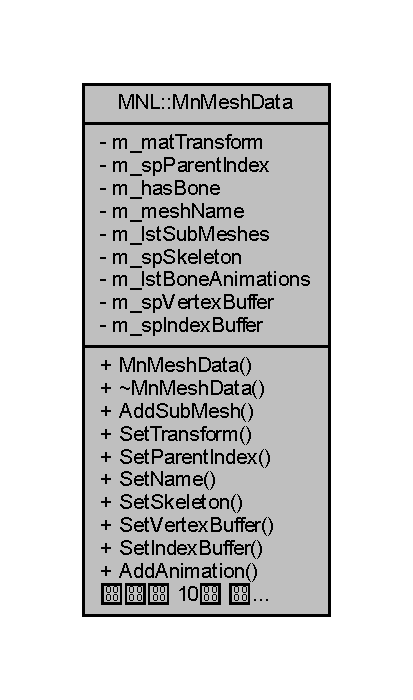
\includegraphics[width=198pt]{class_m_n_l_1_1_mn_mesh_data__coll__graph}
\end{center}
\end{figure}
\subsection*{Public 멤버 함수}
\begin{DoxyCompactItemize}
\item 
\hyperlink{class_m_n_l_1_1_mn_mesh_data_a6012a2d40228be1313a3188b7a1eefcd}{Mn\+Mesh\+Data} ()
\item 
\hyperlink{class_m_n_l_1_1_mn_mesh_data_af1e38c31aa38a1ea459fd68d4be71df7}{$\sim$\+Mn\+Mesh\+Data} ()
\item 
void \hyperlink{class_m_n_l_1_1_mn_mesh_data_acf035cf1ba291fbdd25cf38b856acfc5}{Add\+Sub\+Mesh} (const \hyperlink{struct_m_n_l_1_1_mn_sub_mesh}{Mn\+Sub\+Mesh} \&submesh)
\item 
void \hyperlink{class_m_n_l_1_1_mn_mesh_data_a695340ddfdbf11ba947928702cab7d78}{Set\+Transform} (const Direct\+X\+::\+Simple\+Math\+::\+Matrix \&mat\+Transform)
\item 
void \hyperlink{class_m_n_l_1_1_mn_mesh_data_a4821520088a4e98315269357366c7044}{Set\+Parent\+Index} (U\+I\+NT index)
\item 
void \hyperlink{class_m_n_l_1_1_mn_mesh_data_a75df436523daf783061f4d3752215897}{Set\+Name} (const std\+::string \&name)
\item 
void \hyperlink{class_m_n_l_1_1_mn_mesh_data_a6de0a715ac6d275ebfee31ef6d7e2542}{Set\+Skeleton} (const std\+::shared\+\_\+ptr$<$ \hyperlink{class_m_n_l_1_1_mn_skeleton}{Mn\+Skeleton} $>$ sp\+Skeleton)
\item 
void \hyperlink{class_m_n_l_1_1_mn_mesh_data_a63af26d409c49e637f296419eb60edb4}{Set\+Vertex\+Buffer} (const std\+::shared\+\_\+ptr$<$ \hyperlink{class_m_n_l_1_1_mn_vertex_buffer}{Mn\+Vertex\+Buffer} $>$ sp\+Vertex\+Buffer)
\item 
void \hyperlink{class_m_n_l_1_1_mn_mesh_data_a44e5cc149d2000c081fce11f3a85d1d6}{Set\+Index\+Buffer} (const std\+::shared\+\_\+ptr$<$ \hyperlink{class_m_n_l_1_1_mn_index_buffer}{Mn\+Index\+Buffer} $>$ sp\+Index\+Buffer)
\item 
void \hyperlink{class_m_n_l_1_1_mn_mesh_data_a484dd836ddd1ab819c72a05a6febe554}{Add\+Animation} (const \hyperlink{class_m_n_l_1_1_mn_bone_animation}{Mn\+Bone\+Animation} \&animation)
\item 
bool \hyperlink{class_m_n_l_1_1_mn_mesh_data_a506c6520b99a9e0eba9cf4b2156c275c}{Has\+Bone} () const
\item 
std\+::shared\+\_\+ptr$<$ U\+I\+NT $>$ \hyperlink{class_m_n_l_1_1_mn_mesh_data_a7d8e1da3cec285f2b71c957ab83f1949}{Get\+Parent\+Index} () const
\item 
const std\+::string \& \hyperlink{class_m_n_l_1_1_mn_mesh_data_a3c08b6786c10601909da1cd2da7eb2dd}{Get\+Name} () const
\item 
const std\+::shared\+\_\+ptr$<$ \hyperlink{class_m_n_l_1_1_mn_skeleton}{Mn\+Skeleton} $>$ \hyperlink{class_m_n_l_1_1_mn_mesh_data_adc90604cc77bbdde83e0a539822db40e}{Get\+Skeleton} () const
\item 
const Direct\+X\+::\+Simple\+Math\+::\+Matrix \& \hyperlink{class_m_n_l_1_1_mn_mesh_data_a14d9a6fd189c2c9b0f5c34b3a1aa7ec9}{Get\+Transform} () const
\item 
const std\+::vector$<$ \hyperlink{class_m_n_l_1_1_mn_bone_animation}{Mn\+Bone\+Animation} $>$ \& \hyperlink{class_m_n_l_1_1_mn_mesh_data_a70cb805cb3b13731dd05adaf7730ef83}{Get\+Animations} () const
\item 
std\+::shared\+\_\+ptr$<$ \hyperlink{class_m_n_l_1_1_mn_vertex_buffer}{Mn\+Vertex\+Buffer} $>$ \hyperlink{class_m_n_l_1_1_mn_mesh_data_a63f8b56714a35f4c1dc1a09dc8f936a1}{Get\+Vertex\+Buffer} () const
\item 
std\+::shared\+\_\+ptr$<$ \hyperlink{class_m_n_l_1_1_mn_index_buffer}{Mn\+Index\+Buffer} $>$ \hyperlink{class_m_n_l_1_1_mn_mesh_data_a0d78bd03e4887e4a728f425b099ad1cf}{Get\+Index\+Buffer} () const
\item 
U\+I\+NT \hyperlink{class_m_n_l_1_1_mn_mesh_data_a324ba83139ce03f30f59b616fbd2235a}{Get\+Num\+Sub\+Meshes} () const
\item 
const std\+::vector$<$ \hyperlink{struct_m_n_l_1_1_mn_sub_mesh}{Mn\+Sub\+Mesh} $>$ \& \hyperlink{class_m_n_l_1_1_mn_mesh_data_a15ddb3594a7ead8f11f788a45d00ce59}{Get\+Sub\+Meshes} () const
\end{DoxyCompactItemize}
\subsection*{Private 속성}
\begin{DoxyCompactItemize}
\item 
Direct\+X\+::\+Simple\+Math\+::\+Matrix \hyperlink{class_m_n_l_1_1_mn_mesh_data_a32634c82d36b16309ccd823aad588b9f}{m\+\_\+mat\+Transform}
\item 
std\+::shared\+\_\+ptr$<$ U\+I\+NT $>$ \hyperlink{class_m_n_l_1_1_mn_mesh_data_aa621a08d7f66033a797261bae12a4c18}{m\+\_\+sp\+Parent\+Index}
\item 
bool \hyperlink{class_m_n_l_1_1_mn_mesh_data_a6285c888b6d027103887f2457088fb9b}{m\+\_\+has\+Bone}
\item 
std\+::string \hyperlink{class_m_n_l_1_1_mn_mesh_data_a0d3c6b9633cadd22858273fac2751b26}{m\+\_\+mesh\+Name}
\item 
std\+::vector$<$ \hyperlink{struct_m_n_l_1_1_mn_sub_mesh}{Mn\+Sub\+Mesh} $>$ \hyperlink{class_m_n_l_1_1_mn_mesh_data_ad81b9296d62dcd2d53206f58654b581d}{m\+\_\+lst\+Sub\+Meshes}
\item 
std\+::shared\+\_\+ptr$<$ \hyperlink{class_m_n_l_1_1_mn_skeleton}{Mn\+Skeleton} $>$ \hyperlink{class_m_n_l_1_1_mn_mesh_data_a04f503f266ee9d9a01567c64e3b2367a}{m\+\_\+sp\+Skeleton}
\item 
std\+::vector$<$ \hyperlink{class_m_n_l_1_1_mn_bone_animation}{Mn\+Bone\+Animation} $>$ \hyperlink{class_m_n_l_1_1_mn_mesh_data_aae25c134a51b1baffbc6fe27b9361c62}{m\+\_\+lst\+Bone\+Animations}
\item 
std\+::shared\+\_\+ptr$<$ \hyperlink{class_m_n_l_1_1_mn_vertex_buffer}{Mn\+Vertex\+Buffer} $>$ \hyperlink{class_m_n_l_1_1_mn_mesh_data_aa831d4cca73f55e0c67f47baee413ad3}{m\+\_\+sp\+Vertex\+Buffer}
\item 
std\+::shared\+\_\+ptr$<$ \hyperlink{class_m_n_l_1_1_mn_index_buffer}{Mn\+Index\+Buffer} $>$ \hyperlink{class_m_n_l_1_1_mn_mesh_data_ac16837b09de7b25bd981d168488ed9f1}{m\+\_\+sp\+Index\+Buffer}
\end{DoxyCompactItemize}


\subsection{상세한 설명}


Mn\+Mesh\+Data.\+h 파일의 27 번째 라인에서 정의되었습니다.



\subsection{생성자 \& 소멸자 문서화}
\mbox{\Hypertarget{class_m_n_l_1_1_mn_mesh_data_a6012a2d40228be1313a3188b7a1eefcd}\label{class_m_n_l_1_1_mn_mesh_data_a6012a2d40228be1313a3188b7a1eefcd}} 
\index{M\+N\+L\+::\+Mn\+Mesh\+Data@{M\+N\+L\+::\+Mn\+Mesh\+Data}!Mn\+Mesh\+Data@{Mn\+Mesh\+Data}}
\index{Mn\+Mesh\+Data@{Mn\+Mesh\+Data}!M\+N\+L\+::\+Mn\+Mesh\+Data@{M\+N\+L\+::\+Mn\+Mesh\+Data}}
\subsubsection{\texorpdfstring{Mn\+Mesh\+Data()}{MnMeshData()}}
{\footnotesize\ttfamily Mn\+Mesh\+Data\+::\+Mn\+Mesh\+Data (\begin{DoxyParamCaption}{ }\end{DoxyParamCaption})}



Mn\+Mesh\+Data.\+cpp 파일의 5 번째 라인에서 정의되었습니다.

\mbox{\Hypertarget{class_m_n_l_1_1_mn_mesh_data_af1e38c31aa38a1ea459fd68d4be71df7}\label{class_m_n_l_1_1_mn_mesh_data_af1e38c31aa38a1ea459fd68d4be71df7}} 
\index{M\+N\+L\+::\+Mn\+Mesh\+Data@{M\+N\+L\+::\+Mn\+Mesh\+Data}!````~Mn\+Mesh\+Data@{$\sim$\+Mn\+Mesh\+Data}}
\index{````~Mn\+Mesh\+Data@{$\sim$\+Mn\+Mesh\+Data}!M\+N\+L\+::\+Mn\+Mesh\+Data@{M\+N\+L\+::\+Mn\+Mesh\+Data}}
\subsubsection{\texorpdfstring{$\sim$\+Mn\+Mesh\+Data()}{~MnMeshData()}}
{\footnotesize\ttfamily Mn\+Mesh\+Data\+::$\sim$\+Mn\+Mesh\+Data (\begin{DoxyParamCaption}{ }\end{DoxyParamCaption})}



Mn\+Mesh\+Data.\+cpp 파일의 11 번째 라인에서 정의되었습니다.



\subsection{멤버 함수 문서화}
\mbox{\Hypertarget{class_m_n_l_1_1_mn_mesh_data_a484dd836ddd1ab819c72a05a6febe554}\label{class_m_n_l_1_1_mn_mesh_data_a484dd836ddd1ab819c72a05a6febe554}} 
\index{M\+N\+L\+::\+Mn\+Mesh\+Data@{M\+N\+L\+::\+Mn\+Mesh\+Data}!Add\+Animation@{Add\+Animation}}
\index{Add\+Animation@{Add\+Animation}!M\+N\+L\+::\+Mn\+Mesh\+Data@{M\+N\+L\+::\+Mn\+Mesh\+Data}}
\subsubsection{\texorpdfstring{Add\+Animation()}{AddAnimation()}}
{\footnotesize\ttfamily void Mn\+Mesh\+Data\+::\+Add\+Animation (\begin{DoxyParamCaption}\item[{const \hyperlink{class_m_n_l_1_1_mn_bone_animation}{Mn\+Bone\+Animation} \&}]{animation }\end{DoxyParamCaption})}



Mn\+Mesh\+Data.\+cpp 파일의 44 번째 라인에서 정의되었습니다.

\mbox{\Hypertarget{class_m_n_l_1_1_mn_mesh_data_acf035cf1ba291fbdd25cf38b856acfc5}\label{class_m_n_l_1_1_mn_mesh_data_acf035cf1ba291fbdd25cf38b856acfc5}} 
\index{M\+N\+L\+::\+Mn\+Mesh\+Data@{M\+N\+L\+::\+Mn\+Mesh\+Data}!Add\+Sub\+Mesh@{Add\+Sub\+Mesh}}
\index{Add\+Sub\+Mesh@{Add\+Sub\+Mesh}!M\+N\+L\+::\+Mn\+Mesh\+Data@{M\+N\+L\+::\+Mn\+Mesh\+Data}}
\subsubsection{\texorpdfstring{Add\+Sub\+Mesh()}{AddSubMesh()}}
{\footnotesize\ttfamily void Mn\+Mesh\+Data\+::\+Add\+Sub\+Mesh (\begin{DoxyParamCaption}\item[{const \hyperlink{struct_m_n_l_1_1_mn_sub_mesh}{Mn\+Sub\+Mesh} \&}]{submesh }\end{DoxyParamCaption})}



Mn\+Mesh\+Data.\+cpp 파일의 15 번째 라인에서 정의되었습니다.

\mbox{\Hypertarget{class_m_n_l_1_1_mn_mesh_data_a70cb805cb3b13731dd05adaf7730ef83}\label{class_m_n_l_1_1_mn_mesh_data_a70cb805cb3b13731dd05adaf7730ef83}} 
\index{M\+N\+L\+::\+Mn\+Mesh\+Data@{M\+N\+L\+::\+Mn\+Mesh\+Data}!Get\+Animations@{Get\+Animations}}
\index{Get\+Animations@{Get\+Animations}!M\+N\+L\+::\+Mn\+Mesh\+Data@{M\+N\+L\+::\+Mn\+Mesh\+Data}}
\subsubsection{\texorpdfstring{Get\+Animations()}{GetAnimations()}}
{\footnotesize\ttfamily const std\+::vector$<$ \hyperlink{class_m_n_l_1_1_mn_bone_animation}{Mn\+Bone\+Animation} $>$ \& Mn\+Mesh\+Data\+::\+Get\+Animations (\begin{DoxyParamCaption}{ }\end{DoxyParamCaption}) const}



Mn\+Mesh\+Data.\+cpp 파일의 74 번째 라인에서 정의되었습니다.

\mbox{\Hypertarget{class_m_n_l_1_1_mn_mesh_data_a0d78bd03e4887e4a728f425b099ad1cf}\label{class_m_n_l_1_1_mn_mesh_data_a0d78bd03e4887e4a728f425b099ad1cf}} 
\index{M\+N\+L\+::\+Mn\+Mesh\+Data@{M\+N\+L\+::\+Mn\+Mesh\+Data}!Get\+Index\+Buffer@{Get\+Index\+Buffer}}
\index{Get\+Index\+Buffer@{Get\+Index\+Buffer}!M\+N\+L\+::\+Mn\+Mesh\+Data@{M\+N\+L\+::\+Mn\+Mesh\+Data}}
\subsubsection{\texorpdfstring{Get\+Index\+Buffer()}{GetIndexBuffer()}}
{\footnotesize\ttfamily std\+::shared\+\_\+ptr$<$ \hyperlink{class_m_n_l_1_1_mn_index_buffer}{Mn\+Index\+Buffer} $>$ Mn\+Mesh\+Data\+::\+Get\+Index\+Buffer (\begin{DoxyParamCaption}{ }\end{DoxyParamCaption}) const}



Mn\+Mesh\+Data.\+cpp 파일의 58 번째 라인에서 정의되었습니다.

\mbox{\Hypertarget{class_m_n_l_1_1_mn_mesh_data_a3c08b6786c10601909da1cd2da7eb2dd}\label{class_m_n_l_1_1_mn_mesh_data_a3c08b6786c10601909da1cd2da7eb2dd}} 
\index{M\+N\+L\+::\+Mn\+Mesh\+Data@{M\+N\+L\+::\+Mn\+Mesh\+Data}!Get\+Name@{Get\+Name}}
\index{Get\+Name@{Get\+Name}!M\+N\+L\+::\+Mn\+Mesh\+Data@{M\+N\+L\+::\+Mn\+Mesh\+Data}}
\subsubsection{\texorpdfstring{Get\+Name()}{GetName()}}
{\footnotesize\ttfamily const std\+::string \& Mn\+Mesh\+Data\+::\+Get\+Name (\begin{DoxyParamCaption}{ }\end{DoxyParamCaption}) const}



Mn\+Mesh\+Data.\+cpp 파일의 62 번째 라인에서 정의되었습니다.

\mbox{\Hypertarget{class_m_n_l_1_1_mn_mesh_data_a324ba83139ce03f30f59b616fbd2235a}\label{class_m_n_l_1_1_mn_mesh_data_a324ba83139ce03f30f59b616fbd2235a}} 
\index{M\+N\+L\+::\+Mn\+Mesh\+Data@{M\+N\+L\+::\+Mn\+Mesh\+Data}!Get\+Num\+Sub\+Meshes@{Get\+Num\+Sub\+Meshes}}
\index{Get\+Num\+Sub\+Meshes@{Get\+Num\+Sub\+Meshes}!M\+N\+L\+::\+Mn\+Mesh\+Data@{M\+N\+L\+::\+Mn\+Mesh\+Data}}
\subsubsection{\texorpdfstring{Get\+Num\+Sub\+Meshes()}{GetNumSubMeshes()}}
{\footnotesize\ttfamily U\+I\+NT Mn\+Mesh\+Data\+::\+Get\+Num\+Sub\+Meshes (\begin{DoxyParamCaption}{ }\end{DoxyParamCaption}) const}



Mn\+Mesh\+Data.\+cpp 파일의 82 번째 라인에서 정의되었습니다.

\mbox{\Hypertarget{class_m_n_l_1_1_mn_mesh_data_a7d8e1da3cec285f2b71c957ab83f1949}\label{class_m_n_l_1_1_mn_mesh_data_a7d8e1da3cec285f2b71c957ab83f1949}} 
\index{M\+N\+L\+::\+Mn\+Mesh\+Data@{M\+N\+L\+::\+Mn\+Mesh\+Data}!Get\+Parent\+Index@{Get\+Parent\+Index}}
\index{Get\+Parent\+Index@{Get\+Parent\+Index}!M\+N\+L\+::\+Mn\+Mesh\+Data@{M\+N\+L\+::\+Mn\+Mesh\+Data}}
\subsubsection{\texorpdfstring{Get\+Parent\+Index()}{GetParentIndex()}}
{\footnotesize\ttfamily std\+::shared\+\_\+ptr$<$ U\+I\+NT $>$ Mn\+Mesh\+Data\+::\+Get\+Parent\+Index (\begin{DoxyParamCaption}{ }\end{DoxyParamCaption}) const}



Mn\+Mesh\+Data.\+cpp 파일의 78 번째 라인에서 정의되었습니다.

\mbox{\Hypertarget{class_m_n_l_1_1_mn_mesh_data_adc90604cc77bbdde83e0a539822db40e}\label{class_m_n_l_1_1_mn_mesh_data_adc90604cc77bbdde83e0a539822db40e}} 
\index{M\+N\+L\+::\+Mn\+Mesh\+Data@{M\+N\+L\+::\+Mn\+Mesh\+Data}!Get\+Skeleton@{Get\+Skeleton}}
\index{Get\+Skeleton@{Get\+Skeleton}!M\+N\+L\+::\+Mn\+Mesh\+Data@{M\+N\+L\+::\+Mn\+Mesh\+Data}}
\subsubsection{\texorpdfstring{Get\+Skeleton()}{GetSkeleton()}}
{\footnotesize\ttfamily const std\+::shared\+\_\+ptr$<$ \hyperlink{class_m_n_l_1_1_mn_skeleton}{Mn\+Skeleton} $>$ Mn\+Mesh\+Data\+::\+Get\+Skeleton (\begin{DoxyParamCaption}{ }\end{DoxyParamCaption}) const}



Mn\+Mesh\+Data.\+cpp 파일의 66 번째 라인에서 정의되었습니다.

\mbox{\Hypertarget{class_m_n_l_1_1_mn_mesh_data_a15ddb3594a7ead8f11f788a45d00ce59}\label{class_m_n_l_1_1_mn_mesh_data_a15ddb3594a7ead8f11f788a45d00ce59}} 
\index{M\+N\+L\+::\+Mn\+Mesh\+Data@{M\+N\+L\+::\+Mn\+Mesh\+Data}!Get\+Sub\+Meshes@{Get\+Sub\+Meshes}}
\index{Get\+Sub\+Meshes@{Get\+Sub\+Meshes}!M\+N\+L\+::\+Mn\+Mesh\+Data@{M\+N\+L\+::\+Mn\+Mesh\+Data}}
\subsubsection{\texorpdfstring{Get\+Sub\+Meshes()}{GetSubMeshes()}}
{\footnotesize\ttfamily const std\+::vector$<$ \hyperlink{struct_m_n_l_1_1_mn_sub_mesh}{Mn\+Sub\+Mesh} $>$ \& Mn\+Mesh\+Data\+::\+Get\+Sub\+Meshes (\begin{DoxyParamCaption}{ }\end{DoxyParamCaption}) const}



Mn\+Mesh\+Data.\+cpp 파일의 86 번째 라인에서 정의되었습니다.

\mbox{\Hypertarget{class_m_n_l_1_1_mn_mesh_data_a14d9a6fd189c2c9b0f5c34b3a1aa7ec9}\label{class_m_n_l_1_1_mn_mesh_data_a14d9a6fd189c2c9b0f5c34b3a1aa7ec9}} 
\index{M\+N\+L\+::\+Mn\+Mesh\+Data@{M\+N\+L\+::\+Mn\+Mesh\+Data}!Get\+Transform@{Get\+Transform}}
\index{Get\+Transform@{Get\+Transform}!M\+N\+L\+::\+Mn\+Mesh\+Data@{M\+N\+L\+::\+Mn\+Mesh\+Data}}
\subsubsection{\texorpdfstring{Get\+Transform()}{GetTransform()}}
{\footnotesize\ttfamily const Direct\+X\+::\+Simple\+Math\+::\+Matrix \& Mn\+Mesh\+Data\+::\+Get\+Transform (\begin{DoxyParamCaption}{ }\end{DoxyParamCaption}) const}



Mn\+Mesh\+Data.\+cpp 파일의 70 번째 라인에서 정의되었습니다.

\mbox{\Hypertarget{class_m_n_l_1_1_mn_mesh_data_a63f8b56714a35f4c1dc1a09dc8f936a1}\label{class_m_n_l_1_1_mn_mesh_data_a63f8b56714a35f4c1dc1a09dc8f936a1}} 
\index{M\+N\+L\+::\+Mn\+Mesh\+Data@{M\+N\+L\+::\+Mn\+Mesh\+Data}!Get\+Vertex\+Buffer@{Get\+Vertex\+Buffer}}
\index{Get\+Vertex\+Buffer@{Get\+Vertex\+Buffer}!M\+N\+L\+::\+Mn\+Mesh\+Data@{M\+N\+L\+::\+Mn\+Mesh\+Data}}
\subsubsection{\texorpdfstring{Get\+Vertex\+Buffer()}{GetVertexBuffer()}}
{\footnotesize\ttfamily std\+::shared\+\_\+ptr$<$ \hyperlink{class_m_n_l_1_1_mn_vertex_buffer}{Mn\+Vertex\+Buffer} $>$ Mn\+Mesh\+Data\+::\+Get\+Vertex\+Buffer (\begin{DoxyParamCaption}{ }\end{DoxyParamCaption}) const}



Mn\+Mesh\+Data.\+cpp 파일의 54 번째 라인에서 정의되었습니다.

\mbox{\Hypertarget{class_m_n_l_1_1_mn_mesh_data_a506c6520b99a9e0eba9cf4b2156c275c}\label{class_m_n_l_1_1_mn_mesh_data_a506c6520b99a9e0eba9cf4b2156c275c}} 
\index{M\+N\+L\+::\+Mn\+Mesh\+Data@{M\+N\+L\+::\+Mn\+Mesh\+Data}!Has\+Bone@{Has\+Bone}}
\index{Has\+Bone@{Has\+Bone}!M\+N\+L\+::\+Mn\+Mesh\+Data@{M\+N\+L\+::\+Mn\+Mesh\+Data}}
\subsubsection{\texorpdfstring{Has\+Bone()}{HasBone()}}
{\footnotesize\ttfamily bool Mn\+Mesh\+Data\+::\+Has\+Bone (\begin{DoxyParamCaption}{ }\end{DoxyParamCaption}) const}



Mn\+Mesh\+Data.\+cpp 파일의 49 번째 라인에서 정의되었습니다.

\mbox{\Hypertarget{class_m_n_l_1_1_mn_mesh_data_a44e5cc149d2000c081fce11f3a85d1d6}\label{class_m_n_l_1_1_mn_mesh_data_a44e5cc149d2000c081fce11f3a85d1d6}} 
\index{M\+N\+L\+::\+Mn\+Mesh\+Data@{M\+N\+L\+::\+Mn\+Mesh\+Data}!Set\+Index\+Buffer@{Set\+Index\+Buffer}}
\index{Set\+Index\+Buffer@{Set\+Index\+Buffer}!M\+N\+L\+::\+Mn\+Mesh\+Data@{M\+N\+L\+::\+Mn\+Mesh\+Data}}
\subsubsection{\texorpdfstring{Set\+Index\+Buffer()}{SetIndexBuffer()}}
{\footnotesize\ttfamily void Mn\+Mesh\+Data\+::\+Set\+Index\+Buffer (\begin{DoxyParamCaption}\item[{const std\+::shared\+\_\+ptr$<$ \hyperlink{class_m_n_l_1_1_mn_index_buffer}{Mn\+Index\+Buffer} $>$}]{sp\+Index\+Buffer }\end{DoxyParamCaption})}



Mn\+Mesh\+Data.\+cpp 파일의 40 번째 라인에서 정의되었습니다.

\mbox{\Hypertarget{class_m_n_l_1_1_mn_mesh_data_a75df436523daf783061f4d3752215897}\label{class_m_n_l_1_1_mn_mesh_data_a75df436523daf783061f4d3752215897}} 
\index{M\+N\+L\+::\+Mn\+Mesh\+Data@{M\+N\+L\+::\+Mn\+Mesh\+Data}!Set\+Name@{Set\+Name}}
\index{Set\+Name@{Set\+Name}!M\+N\+L\+::\+Mn\+Mesh\+Data@{M\+N\+L\+::\+Mn\+Mesh\+Data}}
\subsubsection{\texorpdfstring{Set\+Name()}{SetName()}}
{\footnotesize\ttfamily void Mn\+Mesh\+Data\+::\+Set\+Name (\begin{DoxyParamCaption}\item[{const std\+::string \&}]{name }\end{DoxyParamCaption})}



Mn\+Mesh\+Data.\+cpp 파일의 19 번째 라인에서 정의되었습니다.

\mbox{\Hypertarget{class_m_n_l_1_1_mn_mesh_data_a4821520088a4e98315269357366c7044}\label{class_m_n_l_1_1_mn_mesh_data_a4821520088a4e98315269357366c7044}} 
\index{M\+N\+L\+::\+Mn\+Mesh\+Data@{M\+N\+L\+::\+Mn\+Mesh\+Data}!Set\+Parent\+Index@{Set\+Parent\+Index}}
\index{Set\+Parent\+Index@{Set\+Parent\+Index}!M\+N\+L\+::\+Mn\+Mesh\+Data@{M\+N\+L\+::\+Mn\+Mesh\+Data}}
\subsubsection{\texorpdfstring{Set\+Parent\+Index()}{SetParentIndex()}}
{\footnotesize\ttfamily void Mn\+Mesh\+Data\+::\+Set\+Parent\+Index (\begin{DoxyParamCaption}\item[{U\+I\+NT}]{index }\end{DoxyParamCaption})}



Mn\+Mesh\+Data.\+cpp 파일의 31 번째 라인에서 정의되었습니다.

\mbox{\Hypertarget{class_m_n_l_1_1_mn_mesh_data_a6de0a715ac6d275ebfee31ef6d7e2542}\label{class_m_n_l_1_1_mn_mesh_data_a6de0a715ac6d275ebfee31ef6d7e2542}} 
\index{M\+N\+L\+::\+Mn\+Mesh\+Data@{M\+N\+L\+::\+Mn\+Mesh\+Data}!Set\+Skeleton@{Set\+Skeleton}}
\index{Set\+Skeleton@{Set\+Skeleton}!M\+N\+L\+::\+Mn\+Mesh\+Data@{M\+N\+L\+::\+Mn\+Mesh\+Data}}
\subsubsection{\texorpdfstring{Set\+Skeleton()}{SetSkeleton()}}
{\footnotesize\ttfamily void Mn\+Mesh\+Data\+::\+Set\+Skeleton (\begin{DoxyParamCaption}\item[{const std\+::shared\+\_\+ptr$<$ \hyperlink{class_m_n_l_1_1_mn_skeleton}{Mn\+Skeleton} $>$}]{sp\+Skeleton }\end{DoxyParamCaption})}



Mn\+Mesh\+Data.\+cpp 파일의 23 번째 라인에서 정의되었습니다.

\mbox{\Hypertarget{class_m_n_l_1_1_mn_mesh_data_a695340ddfdbf11ba947928702cab7d78}\label{class_m_n_l_1_1_mn_mesh_data_a695340ddfdbf11ba947928702cab7d78}} 
\index{M\+N\+L\+::\+Mn\+Mesh\+Data@{M\+N\+L\+::\+Mn\+Mesh\+Data}!Set\+Transform@{Set\+Transform}}
\index{Set\+Transform@{Set\+Transform}!M\+N\+L\+::\+Mn\+Mesh\+Data@{M\+N\+L\+::\+Mn\+Mesh\+Data}}
\subsubsection{\texorpdfstring{Set\+Transform()}{SetTransform()}}
{\footnotesize\ttfamily void Mn\+Mesh\+Data\+::\+Set\+Transform (\begin{DoxyParamCaption}\item[{const Direct\+X\+::\+Simple\+Math\+::\+Matrix \&}]{mat\+Transform }\end{DoxyParamCaption})}



Mn\+Mesh\+Data.\+cpp 파일의 27 번째 라인에서 정의되었습니다.

\mbox{\Hypertarget{class_m_n_l_1_1_mn_mesh_data_a63af26d409c49e637f296419eb60edb4}\label{class_m_n_l_1_1_mn_mesh_data_a63af26d409c49e637f296419eb60edb4}} 
\index{M\+N\+L\+::\+Mn\+Mesh\+Data@{M\+N\+L\+::\+Mn\+Mesh\+Data}!Set\+Vertex\+Buffer@{Set\+Vertex\+Buffer}}
\index{Set\+Vertex\+Buffer@{Set\+Vertex\+Buffer}!M\+N\+L\+::\+Mn\+Mesh\+Data@{M\+N\+L\+::\+Mn\+Mesh\+Data}}
\subsubsection{\texorpdfstring{Set\+Vertex\+Buffer()}{SetVertexBuffer()}}
{\footnotesize\ttfamily void Mn\+Mesh\+Data\+::\+Set\+Vertex\+Buffer (\begin{DoxyParamCaption}\item[{const std\+::shared\+\_\+ptr$<$ \hyperlink{class_m_n_l_1_1_mn_vertex_buffer}{Mn\+Vertex\+Buffer} $>$}]{sp\+Vertex\+Buffer }\end{DoxyParamCaption})}



Mn\+Mesh\+Data.\+cpp 파일의 36 번째 라인에서 정의되었습니다.



\subsection{멤버 데이터 문서화}
\mbox{\Hypertarget{class_m_n_l_1_1_mn_mesh_data_a6285c888b6d027103887f2457088fb9b}\label{class_m_n_l_1_1_mn_mesh_data_a6285c888b6d027103887f2457088fb9b}} 
\index{M\+N\+L\+::\+Mn\+Mesh\+Data@{M\+N\+L\+::\+Mn\+Mesh\+Data}!m\+\_\+has\+Bone@{m\+\_\+has\+Bone}}
\index{m\+\_\+has\+Bone@{m\+\_\+has\+Bone}!M\+N\+L\+::\+Mn\+Mesh\+Data@{M\+N\+L\+::\+Mn\+Mesh\+Data}}
\subsubsection{\texorpdfstring{m\+\_\+has\+Bone}{m\_hasBone}}
{\footnotesize\ttfamily bool M\+N\+L\+::\+Mn\+Mesh\+Data\+::m\+\_\+has\+Bone\hspace{0.3cm}{\ttfamily [private]}}



Mn\+Mesh\+Data.\+h 파일의 62 번째 라인에서 정의되었습니다.

\mbox{\Hypertarget{class_m_n_l_1_1_mn_mesh_data_aae25c134a51b1baffbc6fe27b9361c62}\label{class_m_n_l_1_1_mn_mesh_data_aae25c134a51b1baffbc6fe27b9361c62}} 
\index{M\+N\+L\+::\+Mn\+Mesh\+Data@{M\+N\+L\+::\+Mn\+Mesh\+Data}!m\+\_\+lst\+Bone\+Animations@{m\+\_\+lst\+Bone\+Animations}}
\index{m\+\_\+lst\+Bone\+Animations@{m\+\_\+lst\+Bone\+Animations}!M\+N\+L\+::\+Mn\+Mesh\+Data@{M\+N\+L\+::\+Mn\+Mesh\+Data}}
\subsubsection{\texorpdfstring{m\+\_\+lst\+Bone\+Animations}{m\_lstBoneAnimations}}
{\footnotesize\ttfamily std\+::vector$<$\hyperlink{class_m_n_l_1_1_mn_bone_animation}{Mn\+Bone\+Animation}$>$ M\+N\+L\+::\+Mn\+Mesh\+Data\+::m\+\_\+lst\+Bone\+Animations\hspace{0.3cm}{\ttfamily [private]}}



Mn\+Mesh\+Data.\+h 파일의 66 번째 라인에서 정의되었습니다.

\mbox{\Hypertarget{class_m_n_l_1_1_mn_mesh_data_ad81b9296d62dcd2d53206f58654b581d}\label{class_m_n_l_1_1_mn_mesh_data_ad81b9296d62dcd2d53206f58654b581d}} 
\index{M\+N\+L\+::\+Mn\+Mesh\+Data@{M\+N\+L\+::\+Mn\+Mesh\+Data}!m\+\_\+lst\+Sub\+Meshes@{m\+\_\+lst\+Sub\+Meshes}}
\index{m\+\_\+lst\+Sub\+Meshes@{m\+\_\+lst\+Sub\+Meshes}!M\+N\+L\+::\+Mn\+Mesh\+Data@{M\+N\+L\+::\+Mn\+Mesh\+Data}}
\subsubsection{\texorpdfstring{m\+\_\+lst\+Sub\+Meshes}{m\_lstSubMeshes}}
{\footnotesize\ttfamily std\+::vector$<$\hyperlink{struct_m_n_l_1_1_mn_sub_mesh}{Mn\+Sub\+Mesh}$>$ M\+N\+L\+::\+Mn\+Mesh\+Data\+::m\+\_\+lst\+Sub\+Meshes\hspace{0.3cm}{\ttfamily [private]}}



Mn\+Mesh\+Data.\+h 파일의 64 번째 라인에서 정의되었습니다.

\mbox{\Hypertarget{class_m_n_l_1_1_mn_mesh_data_a32634c82d36b16309ccd823aad588b9f}\label{class_m_n_l_1_1_mn_mesh_data_a32634c82d36b16309ccd823aad588b9f}} 
\index{M\+N\+L\+::\+Mn\+Mesh\+Data@{M\+N\+L\+::\+Mn\+Mesh\+Data}!m\+\_\+mat\+Transform@{m\+\_\+mat\+Transform}}
\index{m\+\_\+mat\+Transform@{m\+\_\+mat\+Transform}!M\+N\+L\+::\+Mn\+Mesh\+Data@{M\+N\+L\+::\+Mn\+Mesh\+Data}}
\subsubsection{\texorpdfstring{m\+\_\+mat\+Transform}{m\_matTransform}}
{\footnotesize\ttfamily Direct\+X\+::\+Simple\+Math\+::\+Matrix M\+N\+L\+::\+Mn\+Mesh\+Data\+::m\+\_\+mat\+Transform\hspace{0.3cm}{\ttfamily [private]}}



Mn\+Mesh\+Data.\+h 파일의 60 번째 라인에서 정의되었습니다.

\mbox{\Hypertarget{class_m_n_l_1_1_mn_mesh_data_a0d3c6b9633cadd22858273fac2751b26}\label{class_m_n_l_1_1_mn_mesh_data_a0d3c6b9633cadd22858273fac2751b26}} 
\index{M\+N\+L\+::\+Mn\+Mesh\+Data@{M\+N\+L\+::\+Mn\+Mesh\+Data}!m\+\_\+mesh\+Name@{m\+\_\+mesh\+Name}}
\index{m\+\_\+mesh\+Name@{m\+\_\+mesh\+Name}!M\+N\+L\+::\+Mn\+Mesh\+Data@{M\+N\+L\+::\+Mn\+Mesh\+Data}}
\subsubsection{\texorpdfstring{m\+\_\+mesh\+Name}{m\_meshName}}
{\footnotesize\ttfamily std\+::string M\+N\+L\+::\+Mn\+Mesh\+Data\+::m\+\_\+mesh\+Name\hspace{0.3cm}{\ttfamily [private]}}



Mn\+Mesh\+Data.\+h 파일의 63 번째 라인에서 정의되었습니다.

\mbox{\Hypertarget{class_m_n_l_1_1_mn_mesh_data_ac16837b09de7b25bd981d168488ed9f1}\label{class_m_n_l_1_1_mn_mesh_data_ac16837b09de7b25bd981d168488ed9f1}} 
\index{M\+N\+L\+::\+Mn\+Mesh\+Data@{M\+N\+L\+::\+Mn\+Mesh\+Data}!m\+\_\+sp\+Index\+Buffer@{m\+\_\+sp\+Index\+Buffer}}
\index{m\+\_\+sp\+Index\+Buffer@{m\+\_\+sp\+Index\+Buffer}!M\+N\+L\+::\+Mn\+Mesh\+Data@{M\+N\+L\+::\+Mn\+Mesh\+Data}}
\subsubsection{\texorpdfstring{m\+\_\+sp\+Index\+Buffer}{m\_spIndexBuffer}}
{\footnotesize\ttfamily std\+::shared\+\_\+ptr$<$\hyperlink{class_m_n_l_1_1_mn_index_buffer}{Mn\+Index\+Buffer}$>$ M\+N\+L\+::\+Mn\+Mesh\+Data\+::m\+\_\+sp\+Index\+Buffer\hspace{0.3cm}{\ttfamily [private]}}



Mn\+Mesh\+Data.\+h 파일의 71 번째 라인에서 정의되었습니다.

\mbox{\Hypertarget{class_m_n_l_1_1_mn_mesh_data_aa621a08d7f66033a797261bae12a4c18}\label{class_m_n_l_1_1_mn_mesh_data_aa621a08d7f66033a797261bae12a4c18}} 
\index{M\+N\+L\+::\+Mn\+Mesh\+Data@{M\+N\+L\+::\+Mn\+Mesh\+Data}!m\+\_\+sp\+Parent\+Index@{m\+\_\+sp\+Parent\+Index}}
\index{m\+\_\+sp\+Parent\+Index@{m\+\_\+sp\+Parent\+Index}!M\+N\+L\+::\+Mn\+Mesh\+Data@{M\+N\+L\+::\+Mn\+Mesh\+Data}}
\subsubsection{\texorpdfstring{m\+\_\+sp\+Parent\+Index}{m\_spParentIndex}}
{\footnotesize\ttfamily std\+::shared\+\_\+ptr$<$U\+I\+NT$>$ M\+N\+L\+::\+Mn\+Mesh\+Data\+::m\+\_\+sp\+Parent\+Index\hspace{0.3cm}{\ttfamily [private]}}



Mn\+Mesh\+Data.\+h 파일의 61 번째 라인에서 정의되었습니다.

\mbox{\Hypertarget{class_m_n_l_1_1_mn_mesh_data_a04f503f266ee9d9a01567c64e3b2367a}\label{class_m_n_l_1_1_mn_mesh_data_a04f503f266ee9d9a01567c64e3b2367a}} 
\index{M\+N\+L\+::\+Mn\+Mesh\+Data@{M\+N\+L\+::\+Mn\+Mesh\+Data}!m\+\_\+sp\+Skeleton@{m\+\_\+sp\+Skeleton}}
\index{m\+\_\+sp\+Skeleton@{m\+\_\+sp\+Skeleton}!M\+N\+L\+::\+Mn\+Mesh\+Data@{M\+N\+L\+::\+Mn\+Mesh\+Data}}
\subsubsection{\texorpdfstring{m\+\_\+sp\+Skeleton}{m\_spSkeleton}}
{\footnotesize\ttfamily std\+::shared\+\_\+ptr$<$\hyperlink{class_m_n_l_1_1_mn_skeleton}{Mn\+Skeleton}$>$ M\+N\+L\+::\+Mn\+Mesh\+Data\+::m\+\_\+sp\+Skeleton\hspace{0.3cm}{\ttfamily [private]}}



Mn\+Mesh\+Data.\+h 파일의 65 번째 라인에서 정의되었습니다.

\mbox{\Hypertarget{class_m_n_l_1_1_mn_mesh_data_aa831d4cca73f55e0c67f47baee413ad3}\label{class_m_n_l_1_1_mn_mesh_data_aa831d4cca73f55e0c67f47baee413ad3}} 
\index{M\+N\+L\+::\+Mn\+Mesh\+Data@{M\+N\+L\+::\+Mn\+Mesh\+Data}!m\+\_\+sp\+Vertex\+Buffer@{m\+\_\+sp\+Vertex\+Buffer}}
\index{m\+\_\+sp\+Vertex\+Buffer@{m\+\_\+sp\+Vertex\+Buffer}!M\+N\+L\+::\+Mn\+Mesh\+Data@{M\+N\+L\+::\+Mn\+Mesh\+Data}}
\subsubsection{\texorpdfstring{m\+\_\+sp\+Vertex\+Buffer}{m\_spVertexBuffer}}
{\footnotesize\ttfamily std\+::shared\+\_\+ptr$<$\hyperlink{class_m_n_l_1_1_mn_vertex_buffer}{Mn\+Vertex\+Buffer}$>$ M\+N\+L\+::\+Mn\+Mesh\+Data\+::m\+\_\+sp\+Vertex\+Buffer\hspace{0.3cm}{\ttfamily [private]}}



Mn\+Mesh\+Data.\+h 파일의 70 번째 라인에서 정의되었습니다.



이 클래스에 대한 문서화 페이지는 다음의 파일들로부터 생성되었습니다.\+:\begin{DoxyCompactItemize}
\item 
Render/\hyperlink{_mn_mesh_data_8h}{Mn\+Mesh\+Data.\+h}\item 
Render/\hyperlink{_mn_mesh_data_8cpp}{Mn\+Mesh\+Data.\+cpp}\end{DoxyCompactItemize}

\hypertarget{class_m_n_l_1_1_mn_mesh_renderer}{}\section{M\+NL\+:\+:Mn\+Mesh\+Renderer 클래스 참조}
\label{class_m_n_l_1_1_mn_mesh_renderer}\index{M\+N\+L\+::\+Mn\+Mesh\+Renderer@{M\+N\+L\+::\+Mn\+Mesh\+Renderer}}


{\ttfamily \#include $<$Mn\+Mesh\+Renderer.\+h$>$}



M\+NL\+:\+:Mn\+Mesh\+Renderer에 대한 상속 다이어그램 \+: \nopagebreak
\begin{figure}[H]
\begin{center}
\leavevmode
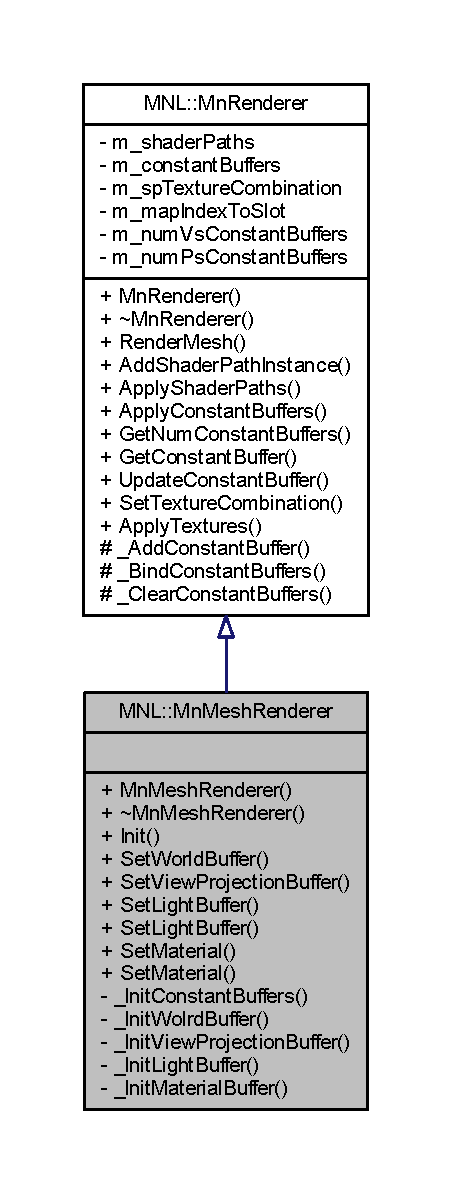
\includegraphics[height=550pt]{class_m_n_l_1_1_mn_mesh_renderer__inherit__graph}
\end{center}
\end{figure}


M\+NL\+:\+:Mn\+Mesh\+Renderer에 대한 협력 다이어그램\+:\nopagebreak
\begin{figure}[H]
\begin{center}
\leavevmode
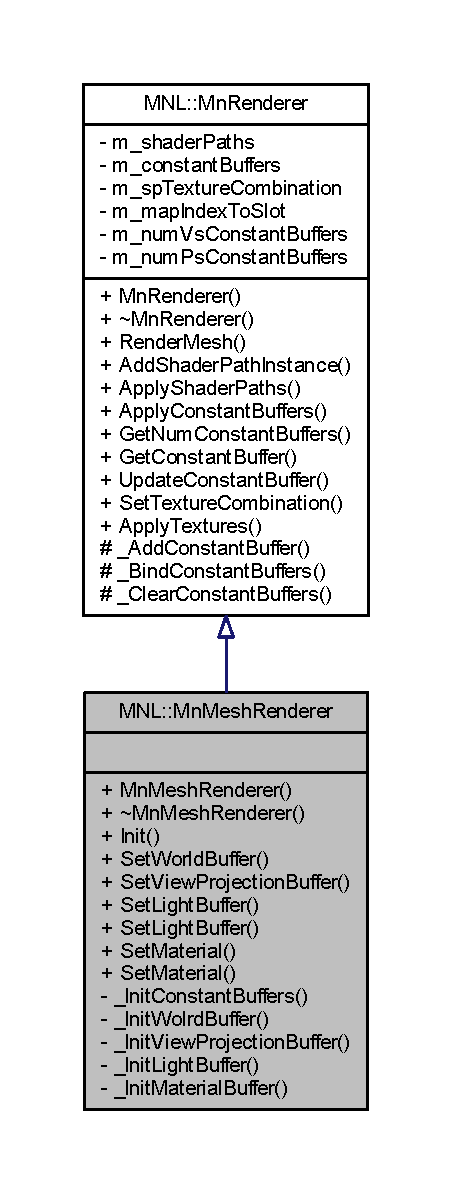
\includegraphics[height=550pt]{class_m_n_l_1_1_mn_mesh_renderer__coll__graph}
\end{center}
\end{figure}
\subsection*{클래스}
\begin{DoxyCompactItemize}
\item 
struct \hyperlink{struct_m_n_l_1_1_mn_mesh_renderer_1_1___light_buffer_type}{\+\_\+\+Light\+Buffer\+Type}
\item 
struct \hyperlink{struct_m_n_l_1_1_mn_mesh_renderer_1_1___material_buffer_type}{\+\_\+\+Material\+Buffer\+Type}
\item 
struct \hyperlink{struct_m_n_l_1_1_mn_mesh_renderer_1_1___view_projection_buffer_type}{\+\_\+\+View\+Projection\+Buffer\+Type}
\item 
struct \hyperlink{struct_m_n_l_1_1_mn_mesh_renderer_1_1___world_buffer_type}{\+\_\+\+World\+Buffer\+Type}
\end{DoxyCompactItemize}
\subsection*{Public 멤버 함수}
\begin{DoxyCompactItemize}
\item 
\hyperlink{class_m_n_l_1_1_mn_mesh_renderer_ab18361a6295007bc68075501ebe12c0a}{Mn\+Mesh\+Renderer} ()
\item 
\hyperlink{class_m_n_l_1_1_mn_mesh_renderer_a35c4902d777cb5e41c7f12eaf54b83f7}{$\sim$\+Mn\+Mesh\+Renderer} ()
\item 
H\+R\+E\+S\+U\+LT \hyperlink{class_m_n_l_1_1_mn_mesh_renderer_ab2f41c8498de2a4470ebbc1adc7e8987}{Init} (const \hyperlink{namespace_m_n_l_a1eec210db8f309a4a9ac0d9658784c31}{C\+P\+D3\+D\+Device} \&cp\+Device, const std\+::shared\+\_\+ptr$<$ \hyperlink{class_m_n_l_1_1_mn_custom_vertex_type}{Mn\+Custom\+Vertex\+Type} $>$ \&sp\+Vertex\+Type)
\item 
void \hyperlink{class_m_n_l_1_1_mn_mesh_renderer_afe78f898609c98523fa7cb1efa52c68f}{Set\+World\+Buffer} (\hyperlink{class_m_n_l_1_1_mn_render_a_p_i}{Mn\+Render\+A\+PI} \&render\+A\+PI, const Direct\+X\+::\+Simple\+Math\+::\+Matrix \&mat\+World)
\item 
void \hyperlink{class_m_n_l_1_1_mn_mesh_renderer_abc60188e28b29f0354aa2ed5ba17fc82}{Set\+View\+Projection\+Buffer} (\hyperlink{class_m_n_l_1_1_mn_render_a_p_i}{Mn\+Render\+A\+PI} \&render\+A\+PI, const Direct\+X\+::\+Simple\+Math\+::\+Matrix \&mat\+View, const Direct\+X\+::\+Simple\+Math\+::\+Matrix \&mat\+Projection)
\item 
void \hyperlink{class_m_n_l_1_1_mn_mesh_renderer_a0c83bc2682917b4504794b510574e320}{Set\+Light\+Buffer} (\hyperlink{class_m_n_l_1_1_mn_render_a_p_i}{Mn\+Render\+A\+PI} \&render\+A\+PI, const Direct\+X\+::\+Simple\+Math\+::\+Vector3 \&light\+Pos, const Direct\+X\+::\+Simple\+Math\+::\+Vector3 \&light\+Dir, \hyperlink{namespace_m_n_l_aac0b78de8bb8c872cb617ede813c113d}{M\+N\+\_\+\+L\+I\+G\+H\+T\+\_\+\+T\+Y\+PE} light\+Type)
\item 
void \hyperlink{class_m_n_l_1_1_mn_mesh_renderer_ad6faf4decf759e6da4ecefa1234aa36e}{Set\+Light\+Buffer} (\hyperlink{class_m_n_l_1_1_mn_render_a_p_i}{Mn\+Render\+A\+PI} \&render\+A\+PI, const std\+::shared\+\_\+ptr$<$ \hyperlink{class_m_n_l_1_1_mn_light_source}{Mn\+Light\+Source} $>$ sp\+Light)
\item 
void \hyperlink{class_m_n_l_1_1_mn_mesh_renderer_ab7ba671fa8776fcd1b8b0de20d7b2f13}{Set\+Material} (\hyperlink{class_m_n_l_1_1_mn_render_a_p_i}{Mn\+Render\+A\+PI} \&render\+A\+PI, const Direct\+X\+::\+Simple\+Math\+::\+Vector4 \&diffuse, const Direct\+X\+::\+Simple\+Math\+::\+Vector4 \&ambient, const Direct\+X\+::\+Simple\+Math\+::\+Vector4 \&emissive, const Direct\+X\+::\+Simple\+Math\+::\+Vector4 \&specular, float specular\+Power)
\item 
void \hyperlink{class_m_n_l_1_1_mn_mesh_renderer_a436b493676e8a9fbc93486a46f6fc58f}{Set\+Material} (\hyperlink{class_m_n_l_1_1_mn_render_a_p_i}{Mn\+Render\+A\+PI} \&render\+A\+PI, const std\+::shared\+\_\+ptr$<$ \hyperlink{class_m_n_l_1_1_mn_material}{Mn\+Material} $>$ sp\+Material)
\end{DoxyCompactItemize}
\subsection*{Private 타입}
\begin{DoxyCompactItemize}
\item 
enum \hyperlink{class_m_n_l_1_1_mn_mesh_renderer_aac99491a7ab8269b32ac0e7d979fc501}{\+\_\+\+C\+O\+N\+S\+T\+\_\+\+B\+U\+F\+F\+E\+RS} \{ \newline
\hyperlink{class_m_n_l_1_1_mn_mesh_renderer_aac99491a7ab8269b32ac0e7d979fc501a33f4ff8f535b64ae9bb0ea7d3ef69871}{\+\_\+\+C\+O\+N\+S\+T\+\_\+\+B\+U\+F\+\_\+\+W\+O\+R\+LD}, 
\hyperlink{class_m_n_l_1_1_mn_mesh_renderer_aac99491a7ab8269b32ac0e7d979fc501ac04be2bcd2f1ee7255a86a8b7411259e}{\+\_\+\+C\+O\+N\+S\+T\+\_\+\+B\+U\+F\+\_\+\+V\+I\+E\+W\+P\+R\+O\+J\+E\+C\+T\+I\+ON}, 
\hyperlink{class_m_n_l_1_1_mn_mesh_renderer_aac99491a7ab8269b32ac0e7d979fc501a497109dcfeb2784ff7a003ea38801d69}{\+\_\+\+C\+O\+N\+S\+T\+\_\+\+B\+U\+F\+\_\+\+L\+I\+G\+H\+T\+\_\+\+VS}, 
\hyperlink{class_m_n_l_1_1_mn_mesh_renderer_aac99491a7ab8269b32ac0e7d979fc501a60a70721d3ad7302c0875daac8bc857c}{\+\_\+\+C\+O\+N\+S\+T\+\_\+\+B\+U\+F\+\_\+\+L\+I\+G\+H\+T\+\_\+\+PS}, 
\newline
\hyperlink{class_m_n_l_1_1_mn_mesh_renderer_aac99491a7ab8269b32ac0e7d979fc501af783c38cca6c4f58231665b8cd2c4191}{\+\_\+\+C\+O\+N\+S\+T\+\_\+\+B\+U\+F\+\_\+\+M\+A\+T\+E\+R\+I\+AL}, 
\hyperlink{class_m_n_l_1_1_mn_mesh_renderer_aac99491a7ab8269b32ac0e7d979fc501ac985c3e52ac24e27c30f1352749b484b}{\+\_\+\+C\+O\+N\+S\+T\+\_\+\+B\+U\+F\+\_\+\+T\+O\+T\+AL}
 \}
\end{DoxyCompactItemize}
\subsection*{Private 멤버 함수}
\begin{DoxyCompactItemize}
\item 
H\+R\+E\+S\+U\+LT \hyperlink{class_m_n_l_1_1_mn_mesh_renderer_ac3396a1345d35c5e52481818eb86b393}{\+\_\+\+Init\+Constant\+Buffers} (const \hyperlink{namespace_m_n_l_a1eec210db8f309a4a9ac0d9658784c31}{C\+P\+D3\+D\+Device} \&cp\+Device)
\item 
H\+R\+E\+S\+U\+LT \hyperlink{class_m_n_l_1_1_mn_mesh_renderer_aba7a3676a4b264a813b64f05e06ac11c}{\+\_\+\+Init\+Wolrd\+Buffer} (const \hyperlink{namespace_m_n_l_a1eec210db8f309a4a9ac0d9658784c31}{C\+P\+D3\+D\+Device} \&cp\+Device)
\item 
H\+R\+E\+S\+U\+LT \hyperlink{class_m_n_l_1_1_mn_mesh_renderer_aa48062a8d90af6b41fc06c6cd4a8dadd}{\+\_\+\+Init\+View\+Projection\+Buffer} (const \hyperlink{namespace_m_n_l_a1eec210db8f309a4a9ac0d9658784c31}{C\+P\+D3\+D\+Device} \&cp\+Device)
\item 
H\+R\+E\+S\+U\+LT \hyperlink{class_m_n_l_1_1_mn_mesh_renderer_a8beea41d6ea1f0061d495ed7cca05926}{\+\_\+\+Init\+Light\+Buffer} (const \hyperlink{namespace_m_n_l_a1eec210db8f309a4a9ac0d9658784c31}{C\+P\+D3\+D\+Device} \&cp\+Device)
\item 
H\+R\+E\+S\+U\+LT \hyperlink{class_m_n_l_1_1_mn_mesh_renderer_a1478d6e5f9244bd15087fa2271a03420}{\+\_\+\+Init\+Material\+Buffer} (const \hyperlink{namespace_m_n_l_a1eec210db8f309a4a9ac0d9658784c31}{C\+P\+D3\+D\+Device} \&cp\+Device)
\end{DoxyCompactItemize}
\subsection*{추가로 상속된 멤버들}


\subsection{상세한 설명}


Mn\+Mesh\+Renderer.\+h 파일의 13 번째 라인에서 정의되었습니다.



\subsection{멤버 열거형 문서화}
\mbox{\Hypertarget{class_m_n_l_1_1_mn_mesh_renderer_aac99491a7ab8269b32ac0e7d979fc501}\label{class_m_n_l_1_1_mn_mesh_renderer_aac99491a7ab8269b32ac0e7d979fc501}} 
\index{M\+N\+L\+::\+Mn\+Mesh\+Renderer@{M\+N\+L\+::\+Mn\+Mesh\+Renderer}!\+\_\+\+C\+O\+N\+S\+T\+\_\+\+B\+U\+F\+F\+E\+RS@{\+\_\+\+C\+O\+N\+S\+T\+\_\+\+B\+U\+F\+F\+E\+RS}}
\index{\+\_\+\+C\+O\+N\+S\+T\+\_\+\+B\+U\+F\+F\+E\+RS@{\+\_\+\+C\+O\+N\+S\+T\+\_\+\+B\+U\+F\+F\+E\+RS}!M\+N\+L\+::\+Mn\+Mesh\+Renderer@{M\+N\+L\+::\+Mn\+Mesh\+Renderer}}
\subsubsection{\texorpdfstring{\+\_\+\+C\+O\+N\+S\+T\+\_\+\+B\+U\+F\+F\+E\+RS}{\_CONST\_BUFFERS}}
{\footnotesize\ttfamily enum \hyperlink{class_m_n_l_1_1_mn_mesh_renderer_aac99491a7ab8269b32ac0e7d979fc501}{M\+N\+L\+::\+Mn\+Mesh\+Renderer\+::\+\_\+\+C\+O\+N\+S\+T\+\_\+\+B\+U\+F\+F\+E\+RS}\hspace{0.3cm}{\ttfamily [private]}}

\begin{DoxyEnumFields}{열거형 멤버}
\raisebox{\heightof{T}}[0pt][0pt]{\index{\+\_\+\+C\+O\+N\+S\+T\+\_\+\+B\+U\+F\+\_\+\+W\+O\+R\+LD@{\+\_\+\+C\+O\+N\+S\+T\+\_\+\+B\+U\+F\+\_\+\+W\+O\+R\+LD}!M\+N\+L\+::\+Mn\+Mesh\+Renderer@{M\+N\+L\+::\+Mn\+Mesh\+Renderer}}\index{M\+N\+L\+::\+Mn\+Mesh\+Renderer@{M\+N\+L\+::\+Mn\+Mesh\+Renderer}!\+\_\+\+C\+O\+N\+S\+T\+\_\+\+B\+U\+F\+\_\+\+W\+O\+R\+LD@{\+\_\+\+C\+O\+N\+S\+T\+\_\+\+B\+U\+F\+\_\+\+W\+O\+R\+LD}}}\mbox{\Hypertarget{class_m_n_l_1_1_mn_mesh_renderer_aac99491a7ab8269b32ac0e7d979fc501a33f4ff8f535b64ae9bb0ea7d3ef69871}\label{class_m_n_l_1_1_mn_mesh_renderer_aac99491a7ab8269b32ac0e7d979fc501a33f4ff8f535b64ae9bb0ea7d3ef69871}} 
\+\_\+\+C\+O\+N\+S\+T\+\_\+\+B\+U\+F\+\_\+\+W\+O\+R\+LD&\\
\hline

\raisebox{\heightof{T}}[0pt][0pt]{\index{\+\_\+\+C\+O\+N\+S\+T\+\_\+\+B\+U\+F\+\_\+\+V\+I\+E\+W\+P\+R\+O\+J\+E\+C\+T\+I\+ON@{\+\_\+\+C\+O\+N\+S\+T\+\_\+\+B\+U\+F\+\_\+\+V\+I\+E\+W\+P\+R\+O\+J\+E\+C\+T\+I\+ON}!M\+N\+L\+::\+Mn\+Mesh\+Renderer@{M\+N\+L\+::\+Mn\+Mesh\+Renderer}}\index{M\+N\+L\+::\+Mn\+Mesh\+Renderer@{M\+N\+L\+::\+Mn\+Mesh\+Renderer}!\+\_\+\+C\+O\+N\+S\+T\+\_\+\+B\+U\+F\+\_\+\+V\+I\+E\+W\+P\+R\+O\+J\+E\+C\+T\+I\+ON@{\+\_\+\+C\+O\+N\+S\+T\+\_\+\+B\+U\+F\+\_\+\+V\+I\+E\+W\+P\+R\+O\+J\+E\+C\+T\+I\+ON}}}\mbox{\Hypertarget{class_m_n_l_1_1_mn_mesh_renderer_aac99491a7ab8269b32ac0e7d979fc501ac04be2bcd2f1ee7255a86a8b7411259e}\label{class_m_n_l_1_1_mn_mesh_renderer_aac99491a7ab8269b32ac0e7d979fc501ac04be2bcd2f1ee7255a86a8b7411259e}} 
\+\_\+\+C\+O\+N\+S\+T\+\_\+\+B\+U\+F\+\_\+\+V\+I\+E\+W\+P\+R\+O\+J\+E\+C\+T\+I\+ON&\\
\hline

\raisebox{\heightof{T}}[0pt][0pt]{\index{\+\_\+\+C\+O\+N\+S\+T\+\_\+\+B\+U\+F\+\_\+\+L\+I\+G\+H\+T\+\_\+\+VS@{\+\_\+\+C\+O\+N\+S\+T\+\_\+\+B\+U\+F\+\_\+\+L\+I\+G\+H\+T\+\_\+\+VS}!M\+N\+L\+::\+Mn\+Mesh\+Renderer@{M\+N\+L\+::\+Mn\+Mesh\+Renderer}}\index{M\+N\+L\+::\+Mn\+Mesh\+Renderer@{M\+N\+L\+::\+Mn\+Mesh\+Renderer}!\+\_\+\+C\+O\+N\+S\+T\+\_\+\+B\+U\+F\+\_\+\+L\+I\+G\+H\+T\+\_\+\+VS@{\+\_\+\+C\+O\+N\+S\+T\+\_\+\+B\+U\+F\+\_\+\+L\+I\+G\+H\+T\+\_\+\+VS}}}\mbox{\Hypertarget{class_m_n_l_1_1_mn_mesh_renderer_aac99491a7ab8269b32ac0e7d979fc501a497109dcfeb2784ff7a003ea38801d69}\label{class_m_n_l_1_1_mn_mesh_renderer_aac99491a7ab8269b32ac0e7d979fc501a497109dcfeb2784ff7a003ea38801d69}} 
\+\_\+\+C\+O\+N\+S\+T\+\_\+\+B\+U\+F\+\_\+\+L\+I\+G\+H\+T\+\_\+\+VS&\\
\hline

\raisebox{\heightof{T}}[0pt][0pt]{\index{\+\_\+\+C\+O\+N\+S\+T\+\_\+\+B\+U\+F\+\_\+\+L\+I\+G\+H\+T\+\_\+\+PS@{\+\_\+\+C\+O\+N\+S\+T\+\_\+\+B\+U\+F\+\_\+\+L\+I\+G\+H\+T\+\_\+\+PS}!M\+N\+L\+::\+Mn\+Mesh\+Renderer@{M\+N\+L\+::\+Mn\+Mesh\+Renderer}}\index{M\+N\+L\+::\+Mn\+Mesh\+Renderer@{M\+N\+L\+::\+Mn\+Mesh\+Renderer}!\+\_\+\+C\+O\+N\+S\+T\+\_\+\+B\+U\+F\+\_\+\+L\+I\+G\+H\+T\+\_\+\+PS@{\+\_\+\+C\+O\+N\+S\+T\+\_\+\+B\+U\+F\+\_\+\+L\+I\+G\+H\+T\+\_\+\+PS}}}\mbox{\Hypertarget{class_m_n_l_1_1_mn_mesh_renderer_aac99491a7ab8269b32ac0e7d979fc501a60a70721d3ad7302c0875daac8bc857c}\label{class_m_n_l_1_1_mn_mesh_renderer_aac99491a7ab8269b32ac0e7d979fc501a60a70721d3ad7302c0875daac8bc857c}} 
\+\_\+\+C\+O\+N\+S\+T\+\_\+\+B\+U\+F\+\_\+\+L\+I\+G\+H\+T\+\_\+\+PS&\\
\hline

\raisebox{\heightof{T}}[0pt][0pt]{\index{\+\_\+\+C\+O\+N\+S\+T\+\_\+\+B\+U\+F\+\_\+\+M\+A\+T\+E\+R\+I\+AL@{\+\_\+\+C\+O\+N\+S\+T\+\_\+\+B\+U\+F\+\_\+\+M\+A\+T\+E\+R\+I\+AL}!M\+N\+L\+::\+Mn\+Mesh\+Renderer@{M\+N\+L\+::\+Mn\+Mesh\+Renderer}}\index{M\+N\+L\+::\+Mn\+Mesh\+Renderer@{M\+N\+L\+::\+Mn\+Mesh\+Renderer}!\+\_\+\+C\+O\+N\+S\+T\+\_\+\+B\+U\+F\+\_\+\+M\+A\+T\+E\+R\+I\+AL@{\+\_\+\+C\+O\+N\+S\+T\+\_\+\+B\+U\+F\+\_\+\+M\+A\+T\+E\+R\+I\+AL}}}\mbox{\Hypertarget{class_m_n_l_1_1_mn_mesh_renderer_aac99491a7ab8269b32ac0e7d979fc501af783c38cca6c4f58231665b8cd2c4191}\label{class_m_n_l_1_1_mn_mesh_renderer_aac99491a7ab8269b32ac0e7d979fc501af783c38cca6c4f58231665b8cd2c4191}} 
\+\_\+\+C\+O\+N\+S\+T\+\_\+\+B\+U\+F\+\_\+\+M\+A\+T\+E\+R\+I\+AL&\\
\hline

\raisebox{\heightof{T}}[0pt][0pt]{\index{\+\_\+\+C\+O\+N\+S\+T\+\_\+\+B\+U\+F\+\_\+\+T\+O\+T\+AL@{\+\_\+\+C\+O\+N\+S\+T\+\_\+\+B\+U\+F\+\_\+\+T\+O\+T\+AL}!M\+N\+L\+::\+Mn\+Mesh\+Renderer@{M\+N\+L\+::\+Mn\+Mesh\+Renderer}}\index{M\+N\+L\+::\+Mn\+Mesh\+Renderer@{M\+N\+L\+::\+Mn\+Mesh\+Renderer}!\+\_\+\+C\+O\+N\+S\+T\+\_\+\+B\+U\+F\+\_\+\+T\+O\+T\+AL@{\+\_\+\+C\+O\+N\+S\+T\+\_\+\+B\+U\+F\+\_\+\+T\+O\+T\+AL}}}\mbox{\Hypertarget{class_m_n_l_1_1_mn_mesh_renderer_aac99491a7ab8269b32ac0e7d979fc501ac985c3e52ac24e27c30f1352749b484b}\label{class_m_n_l_1_1_mn_mesh_renderer_aac99491a7ab8269b32ac0e7d979fc501ac985c3e52ac24e27c30f1352749b484b}} 
\+\_\+\+C\+O\+N\+S\+T\+\_\+\+B\+U\+F\+\_\+\+T\+O\+T\+AL&\\
\hline

\end{DoxyEnumFields}


Mn\+Mesh\+Renderer.\+h 파일의 20 번째 라인에서 정의되었습니다.



\subsection{생성자 \& 소멸자 문서화}
\mbox{\Hypertarget{class_m_n_l_1_1_mn_mesh_renderer_ab18361a6295007bc68075501ebe12c0a}\label{class_m_n_l_1_1_mn_mesh_renderer_ab18361a6295007bc68075501ebe12c0a}} 
\index{M\+N\+L\+::\+Mn\+Mesh\+Renderer@{M\+N\+L\+::\+Mn\+Mesh\+Renderer}!Mn\+Mesh\+Renderer@{Mn\+Mesh\+Renderer}}
\index{Mn\+Mesh\+Renderer@{Mn\+Mesh\+Renderer}!M\+N\+L\+::\+Mn\+Mesh\+Renderer@{M\+N\+L\+::\+Mn\+Mesh\+Renderer}}
\subsubsection{\texorpdfstring{Mn\+Mesh\+Renderer()}{MnMeshRenderer()}}
{\footnotesize\ttfamily Mn\+Mesh\+Renderer\+::\+Mn\+Mesh\+Renderer (\begin{DoxyParamCaption}{ }\end{DoxyParamCaption})}



Mn\+Mesh\+Renderer.\+cpp 파일의 7 번째 라인에서 정의되었습니다.

\mbox{\Hypertarget{class_m_n_l_1_1_mn_mesh_renderer_a35c4902d777cb5e41c7f12eaf54b83f7}\label{class_m_n_l_1_1_mn_mesh_renderer_a35c4902d777cb5e41c7f12eaf54b83f7}} 
\index{M\+N\+L\+::\+Mn\+Mesh\+Renderer@{M\+N\+L\+::\+Mn\+Mesh\+Renderer}!````~Mn\+Mesh\+Renderer@{$\sim$\+Mn\+Mesh\+Renderer}}
\index{````~Mn\+Mesh\+Renderer@{$\sim$\+Mn\+Mesh\+Renderer}!M\+N\+L\+::\+Mn\+Mesh\+Renderer@{M\+N\+L\+::\+Mn\+Mesh\+Renderer}}
\subsubsection{\texorpdfstring{$\sim$\+Mn\+Mesh\+Renderer()}{~MnMeshRenderer()}}
{\footnotesize\ttfamily Mn\+Mesh\+Renderer\+::$\sim$\+Mn\+Mesh\+Renderer (\begin{DoxyParamCaption}{ }\end{DoxyParamCaption})}



Mn\+Mesh\+Renderer.\+cpp 파일의 12 번째 라인에서 정의되었습니다.



\subsection{멤버 함수 문서화}
\mbox{\Hypertarget{class_m_n_l_1_1_mn_mesh_renderer_ac3396a1345d35c5e52481818eb86b393}\label{class_m_n_l_1_1_mn_mesh_renderer_ac3396a1345d35c5e52481818eb86b393}} 
\index{M\+N\+L\+::\+Mn\+Mesh\+Renderer@{M\+N\+L\+::\+Mn\+Mesh\+Renderer}!\+\_\+\+Init\+Constant\+Buffers@{\+\_\+\+Init\+Constant\+Buffers}}
\index{\+\_\+\+Init\+Constant\+Buffers@{\+\_\+\+Init\+Constant\+Buffers}!M\+N\+L\+::\+Mn\+Mesh\+Renderer@{M\+N\+L\+::\+Mn\+Mesh\+Renderer}}
\subsubsection{\texorpdfstring{\+\_\+\+Init\+Constant\+Buffers()}{\_InitConstantBuffers()}}
{\footnotesize\ttfamily H\+R\+E\+S\+U\+LT Mn\+Mesh\+Renderer\+::\+\_\+\+Init\+Constant\+Buffers (\begin{DoxyParamCaption}\item[{const \hyperlink{namespace_m_n_l_a1eec210db8f309a4a9ac0d9658784c31}{C\+P\+D3\+D\+Device} \&}]{cp\+Device }\end{DoxyParamCaption})\hspace{0.3cm}{\ttfamily [private]}}



Mn\+Mesh\+Renderer.\+cpp 파일의 107 번째 라인에서 정의되었습니다.

\mbox{\Hypertarget{class_m_n_l_1_1_mn_mesh_renderer_a8beea41d6ea1f0061d495ed7cca05926}\label{class_m_n_l_1_1_mn_mesh_renderer_a8beea41d6ea1f0061d495ed7cca05926}} 
\index{M\+N\+L\+::\+Mn\+Mesh\+Renderer@{M\+N\+L\+::\+Mn\+Mesh\+Renderer}!\+\_\+\+Init\+Light\+Buffer@{\+\_\+\+Init\+Light\+Buffer}}
\index{\+\_\+\+Init\+Light\+Buffer@{\+\_\+\+Init\+Light\+Buffer}!M\+N\+L\+::\+Mn\+Mesh\+Renderer@{M\+N\+L\+::\+Mn\+Mesh\+Renderer}}
\subsubsection{\texorpdfstring{\+\_\+\+Init\+Light\+Buffer()}{\_InitLightBuffer()}}
{\footnotesize\ttfamily H\+R\+E\+S\+U\+LT Mn\+Mesh\+Renderer\+::\+\_\+\+Init\+Light\+Buffer (\begin{DoxyParamCaption}\item[{const \hyperlink{namespace_m_n_l_a1eec210db8f309a4a9ac0d9658784c31}{C\+P\+D3\+D\+Device} \&}]{cp\+Device }\end{DoxyParamCaption})\hspace{0.3cm}{\ttfamily [private]}}



Mn\+Mesh\+Renderer.\+cpp 파일의 183 번째 라인에서 정의되었습니다.

\mbox{\Hypertarget{class_m_n_l_1_1_mn_mesh_renderer_a1478d6e5f9244bd15087fa2271a03420}\label{class_m_n_l_1_1_mn_mesh_renderer_a1478d6e5f9244bd15087fa2271a03420}} 
\index{M\+N\+L\+::\+Mn\+Mesh\+Renderer@{M\+N\+L\+::\+Mn\+Mesh\+Renderer}!\+\_\+\+Init\+Material\+Buffer@{\+\_\+\+Init\+Material\+Buffer}}
\index{\+\_\+\+Init\+Material\+Buffer@{\+\_\+\+Init\+Material\+Buffer}!M\+N\+L\+::\+Mn\+Mesh\+Renderer@{M\+N\+L\+::\+Mn\+Mesh\+Renderer}}
\subsubsection{\texorpdfstring{\+\_\+\+Init\+Material\+Buffer()}{\_InitMaterialBuffer()}}
{\footnotesize\ttfamily H\+R\+E\+S\+U\+LT Mn\+Mesh\+Renderer\+::\+\_\+\+Init\+Material\+Buffer (\begin{DoxyParamCaption}\item[{const \hyperlink{namespace_m_n_l_a1eec210db8f309a4a9ac0d9658784c31}{C\+P\+D3\+D\+Device} \&}]{cp\+Device }\end{DoxyParamCaption})\hspace{0.3cm}{\ttfamily [private]}}



Mn\+Mesh\+Renderer.\+cpp 파일의 218 번째 라인에서 정의되었습니다.

\mbox{\Hypertarget{class_m_n_l_1_1_mn_mesh_renderer_aa48062a8d90af6b41fc06c6cd4a8dadd}\label{class_m_n_l_1_1_mn_mesh_renderer_aa48062a8d90af6b41fc06c6cd4a8dadd}} 
\index{M\+N\+L\+::\+Mn\+Mesh\+Renderer@{M\+N\+L\+::\+Mn\+Mesh\+Renderer}!\+\_\+\+Init\+View\+Projection\+Buffer@{\+\_\+\+Init\+View\+Projection\+Buffer}}
\index{\+\_\+\+Init\+View\+Projection\+Buffer@{\+\_\+\+Init\+View\+Projection\+Buffer}!M\+N\+L\+::\+Mn\+Mesh\+Renderer@{M\+N\+L\+::\+Mn\+Mesh\+Renderer}}
\subsubsection{\texorpdfstring{\+\_\+\+Init\+View\+Projection\+Buffer()}{\_InitViewProjectionBuffer()}}
{\footnotesize\ttfamily H\+R\+E\+S\+U\+LT Mn\+Mesh\+Renderer\+::\+\_\+\+Init\+View\+Projection\+Buffer (\begin{DoxyParamCaption}\item[{const \hyperlink{namespace_m_n_l_a1eec210db8f309a4a9ac0d9658784c31}{C\+P\+D3\+D\+Device} \&}]{cp\+Device }\end{DoxyParamCaption})\hspace{0.3cm}{\ttfamily [private]}}



Mn\+Mesh\+Renderer.\+cpp 파일의 163 번째 라인에서 정의되었습니다.

\mbox{\Hypertarget{class_m_n_l_1_1_mn_mesh_renderer_aba7a3676a4b264a813b64f05e06ac11c}\label{class_m_n_l_1_1_mn_mesh_renderer_aba7a3676a4b264a813b64f05e06ac11c}} 
\index{M\+N\+L\+::\+Mn\+Mesh\+Renderer@{M\+N\+L\+::\+Mn\+Mesh\+Renderer}!\+\_\+\+Init\+Wolrd\+Buffer@{\+\_\+\+Init\+Wolrd\+Buffer}}
\index{\+\_\+\+Init\+Wolrd\+Buffer@{\+\_\+\+Init\+Wolrd\+Buffer}!M\+N\+L\+::\+Mn\+Mesh\+Renderer@{M\+N\+L\+::\+Mn\+Mesh\+Renderer}}
\subsubsection{\texorpdfstring{\+\_\+\+Init\+Wolrd\+Buffer()}{\_InitWolrdBuffer()}}
{\footnotesize\ttfamily H\+R\+E\+S\+U\+LT Mn\+Mesh\+Renderer\+::\+\_\+\+Init\+Wolrd\+Buffer (\begin{DoxyParamCaption}\item[{const \hyperlink{namespace_m_n_l_a1eec210db8f309a4a9ac0d9658784c31}{C\+P\+D3\+D\+Device} \&}]{cp\+Device }\end{DoxyParamCaption})\hspace{0.3cm}{\ttfamily [private]}}



Mn\+Mesh\+Renderer.\+cpp 파일의 143 번째 라인에서 정의되었습니다.

\mbox{\Hypertarget{class_m_n_l_1_1_mn_mesh_renderer_ab2f41c8498de2a4470ebbc1adc7e8987}\label{class_m_n_l_1_1_mn_mesh_renderer_ab2f41c8498de2a4470ebbc1adc7e8987}} 
\index{M\+N\+L\+::\+Mn\+Mesh\+Renderer@{M\+N\+L\+::\+Mn\+Mesh\+Renderer}!Init@{Init}}
\index{Init@{Init}!M\+N\+L\+::\+Mn\+Mesh\+Renderer@{M\+N\+L\+::\+Mn\+Mesh\+Renderer}}
\subsubsection{\texorpdfstring{Init()}{Init()}}
{\footnotesize\ttfamily H\+R\+E\+S\+U\+LT Mn\+Mesh\+Renderer\+::\+Init (\begin{DoxyParamCaption}\item[{const \hyperlink{namespace_m_n_l_a1eec210db8f309a4a9ac0d9658784c31}{C\+P\+D3\+D\+Device} \&}]{cp\+Device,  }\item[{const std\+::shared\+\_\+ptr$<$ \hyperlink{class_m_n_l_1_1_mn_custom_vertex_type}{Mn\+Custom\+Vertex\+Type} $>$ \&}]{sp\+Vertex\+Type }\end{DoxyParamCaption})}



Mn\+Mesh\+Renderer.\+cpp 파일의 17 번째 라인에서 정의되었습니다.

\mbox{\Hypertarget{class_m_n_l_1_1_mn_mesh_renderer_a0c83bc2682917b4504794b510574e320}\label{class_m_n_l_1_1_mn_mesh_renderer_a0c83bc2682917b4504794b510574e320}} 
\index{M\+N\+L\+::\+Mn\+Mesh\+Renderer@{M\+N\+L\+::\+Mn\+Mesh\+Renderer}!Set\+Light\+Buffer@{Set\+Light\+Buffer}}
\index{Set\+Light\+Buffer@{Set\+Light\+Buffer}!M\+N\+L\+::\+Mn\+Mesh\+Renderer@{M\+N\+L\+::\+Mn\+Mesh\+Renderer}}
\subsubsection{\texorpdfstring{Set\+Light\+Buffer()}{SetLightBuffer()}\hspace{0.1cm}{\footnotesize\ttfamily [1/2]}}
{\footnotesize\ttfamily void Mn\+Mesh\+Renderer\+::\+Set\+Light\+Buffer (\begin{DoxyParamCaption}\item[{\hyperlink{class_m_n_l_1_1_mn_render_a_p_i}{Mn\+Render\+A\+PI} \&}]{render\+A\+PI,  }\item[{const Direct\+X\+::\+Simple\+Math\+::\+Vector3 \&}]{light\+Pos,  }\item[{const Direct\+X\+::\+Simple\+Math\+::\+Vector3 \&}]{light\+Dir,  }\item[{\hyperlink{namespace_m_n_l_aac0b78de8bb8c872cb617ede813c113d}{M\+N\+\_\+\+L\+I\+G\+H\+T\+\_\+\+T\+Y\+PE}}]{light\+Type }\end{DoxyParamCaption})}



Mn\+Mesh\+Renderer.\+cpp 파일의 59 번째 라인에서 정의되었습니다.

\mbox{\Hypertarget{class_m_n_l_1_1_mn_mesh_renderer_ad6faf4decf759e6da4ecefa1234aa36e}\label{class_m_n_l_1_1_mn_mesh_renderer_ad6faf4decf759e6da4ecefa1234aa36e}} 
\index{M\+N\+L\+::\+Mn\+Mesh\+Renderer@{M\+N\+L\+::\+Mn\+Mesh\+Renderer}!Set\+Light\+Buffer@{Set\+Light\+Buffer}}
\index{Set\+Light\+Buffer@{Set\+Light\+Buffer}!M\+N\+L\+::\+Mn\+Mesh\+Renderer@{M\+N\+L\+::\+Mn\+Mesh\+Renderer}}
\subsubsection{\texorpdfstring{Set\+Light\+Buffer()}{SetLightBuffer()}\hspace{0.1cm}{\footnotesize\ttfamily [2/2]}}
{\footnotesize\ttfamily void Mn\+Mesh\+Renderer\+::\+Set\+Light\+Buffer (\begin{DoxyParamCaption}\item[{\hyperlink{class_m_n_l_1_1_mn_render_a_p_i}{Mn\+Render\+A\+PI} \&}]{render\+A\+PI,  }\item[{const std\+::shared\+\_\+ptr$<$ \hyperlink{class_m_n_l_1_1_mn_light_source}{Mn\+Light\+Source} $>$}]{sp\+Light }\end{DoxyParamCaption})}



Mn\+Mesh\+Renderer.\+cpp 파일의 75 번째 라인에서 정의되었습니다.

\mbox{\Hypertarget{class_m_n_l_1_1_mn_mesh_renderer_ab7ba671fa8776fcd1b8b0de20d7b2f13}\label{class_m_n_l_1_1_mn_mesh_renderer_ab7ba671fa8776fcd1b8b0de20d7b2f13}} 
\index{M\+N\+L\+::\+Mn\+Mesh\+Renderer@{M\+N\+L\+::\+Mn\+Mesh\+Renderer}!Set\+Material@{Set\+Material}}
\index{Set\+Material@{Set\+Material}!M\+N\+L\+::\+Mn\+Mesh\+Renderer@{M\+N\+L\+::\+Mn\+Mesh\+Renderer}}
\subsubsection{\texorpdfstring{Set\+Material()}{SetMaterial()}\hspace{0.1cm}{\footnotesize\ttfamily [1/2]}}
{\footnotesize\ttfamily void Mn\+Mesh\+Renderer\+::\+Set\+Material (\begin{DoxyParamCaption}\item[{\hyperlink{class_m_n_l_1_1_mn_render_a_p_i}{Mn\+Render\+A\+PI} \&}]{render\+A\+PI,  }\item[{const Direct\+X\+::\+Simple\+Math\+::\+Vector4 \&}]{diffuse,  }\item[{const Direct\+X\+::\+Simple\+Math\+::\+Vector4 \&}]{ambient,  }\item[{const Direct\+X\+::\+Simple\+Math\+::\+Vector4 \&}]{emissive,  }\item[{const Direct\+X\+::\+Simple\+Math\+::\+Vector4 \&}]{specular,  }\item[{float}]{specular\+Power }\end{DoxyParamCaption})}



Mn\+Mesh\+Renderer.\+cpp 파일의 80 번째 라인에서 정의되었습니다.

\mbox{\Hypertarget{class_m_n_l_1_1_mn_mesh_renderer_a436b493676e8a9fbc93486a46f6fc58f}\label{class_m_n_l_1_1_mn_mesh_renderer_a436b493676e8a9fbc93486a46f6fc58f}} 
\index{M\+N\+L\+::\+Mn\+Mesh\+Renderer@{M\+N\+L\+::\+Mn\+Mesh\+Renderer}!Set\+Material@{Set\+Material}}
\index{Set\+Material@{Set\+Material}!M\+N\+L\+::\+Mn\+Mesh\+Renderer@{M\+N\+L\+::\+Mn\+Mesh\+Renderer}}
\subsubsection{\texorpdfstring{Set\+Material()}{SetMaterial()}\hspace{0.1cm}{\footnotesize\ttfamily [2/2]}}
{\footnotesize\ttfamily void Mn\+Mesh\+Renderer\+::\+Set\+Material (\begin{DoxyParamCaption}\item[{\hyperlink{class_m_n_l_1_1_mn_render_a_p_i}{Mn\+Render\+A\+PI} \&}]{render\+A\+PI,  }\item[{const std\+::shared\+\_\+ptr$<$ \hyperlink{class_m_n_l_1_1_mn_material}{Mn\+Material} $>$}]{sp\+Material }\end{DoxyParamCaption})}



Mn\+Mesh\+Renderer.\+cpp 파일의 102 번째 라인에서 정의되었습니다.

\mbox{\Hypertarget{class_m_n_l_1_1_mn_mesh_renderer_abc60188e28b29f0354aa2ed5ba17fc82}\label{class_m_n_l_1_1_mn_mesh_renderer_abc60188e28b29f0354aa2ed5ba17fc82}} 
\index{M\+N\+L\+::\+Mn\+Mesh\+Renderer@{M\+N\+L\+::\+Mn\+Mesh\+Renderer}!Set\+View\+Projection\+Buffer@{Set\+View\+Projection\+Buffer}}
\index{Set\+View\+Projection\+Buffer@{Set\+View\+Projection\+Buffer}!M\+N\+L\+::\+Mn\+Mesh\+Renderer@{M\+N\+L\+::\+Mn\+Mesh\+Renderer}}
\subsubsection{\texorpdfstring{Set\+View\+Projection\+Buffer()}{SetViewProjectionBuffer()}}
{\footnotesize\ttfamily void Mn\+Mesh\+Renderer\+::\+Set\+View\+Projection\+Buffer (\begin{DoxyParamCaption}\item[{\hyperlink{class_m_n_l_1_1_mn_render_a_p_i}{Mn\+Render\+A\+PI} \&}]{render\+A\+PI,  }\item[{const Direct\+X\+::\+Simple\+Math\+::\+Matrix \&}]{mat\+View,  }\item[{const Direct\+X\+::\+Simple\+Math\+::\+Matrix \&}]{mat\+Projection }\end{DoxyParamCaption})}



Mn\+Mesh\+Renderer.\+cpp 파일의 43 번째 라인에서 정의되었습니다.

\mbox{\Hypertarget{class_m_n_l_1_1_mn_mesh_renderer_afe78f898609c98523fa7cb1efa52c68f}\label{class_m_n_l_1_1_mn_mesh_renderer_afe78f898609c98523fa7cb1efa52c68f}} 
\index{M\+N\+L\+::\+Mn\+Mesh\+Renderer@{M\+N\+L\+::\+Mn\+Mesh\+Renderer}!Set\+World\+Buffer@{Set\+World\+Buffer}}
\index{Set\+World\+Buffer@{Set\+World\+Buffer}!M\+N\+L\+::\+Mn\+Mesh\+Renderer@{M\+N\+L\+::\+Mn\+Mesh\+Renderer}}
\subsubsection{\texorpdfstring{Set\+World\+Buffer()}{SetWorldBuffer()}}
{\footnotesize\ttfamily void Mn\+Mesh\+Renderer\+::\+Set\+World\+Buffer (\begin{DoxyParamCaption}\item[{\hyperlink{class_m_n_l_1_1_mn_render_a_p_i}{Mn\+Render\+A\+PI} \&}]{render\+A\+PI,  }\item[{const Direct\+X\+::\+Simple\+Math\+::\+Matrix \&}]{mat\+World }\end{DoxyParamCaption})}



Mn\+Mesh\+Renderer.\+cpp 파일의 28 번째 라인에서 정의되었습니다.



이 클래스에 대한 문서화 페이지는 다음의 파일들로부터 생성되었습니다.\+:\begin{DoxyCompactItemize}
\item 
Render/\hyperlink{_mn_mesh_renderer_8h}{Mn\+Mesh\+Renderer.\+h}\item 
Render/\hyperlink{_mn_mesh_renderer_8cpp}{Mn\+Mesh\+Renderer.\+cpp}\end{DoxyCompactItemize}

\hypertarget{class_m_n_l_1_1_mn_mesh_texture}{}\section{M\+NL\+:\+:Mn\+Mesh\+Texture 클래스 참조}
\label{class_m_n_l_1_1_mn_mesh_texture}\index{M\+N\+L\+::\+Mn\+Mesh\+Texture@{M\+N\+L\+::\+Mn\+Mesh\+Texture}}


{\ttfamily \#include $<$Mn\+Mesh\+Texture.\+h$>$}



M\+NL\+:\+:Mn\+Mesh\+Texture에 대한 협력 다이어그램\+:\nopagebreak
\begin{figure}[H]
\begin{center}
\leavevmode
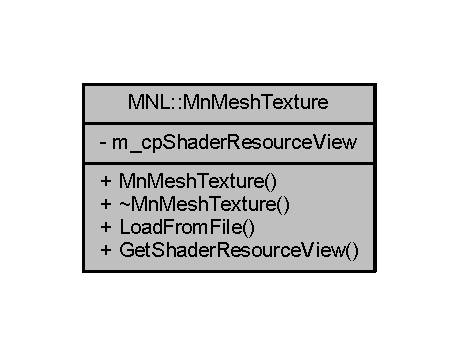
\includegraphics[width=220pt]{class_m_n_l_1_1_mn_mesh_texture__coll__graph}
\end{center}
\end{figure}
\subsection*{Public 멤버 함수}
\begin{DoxyCompactItemize}
\item 
\hyperlink{class_m_n_l_1_1_mn_mesh_texture_ac29132ecef67120fbcb9f5f34abfe24a}{Mn\+Mesh\+Texture} ()
\item 
\hyperlink{class_m_n_l_1_1_mn_mesh_texture_ae49980cf93b9164685c8c569335f16d8}{$\sim$\+Mn\+Mesh\+Texture} ()
\item 
H\+R\+E\+S\+U\+LT \hyperlink{class_m_n_l_1_1_mn_mesh_texture_acd57364c25a3304f5f80cdd2f2ff310d}{Load\+From\+File} (const \hyperlink{namespace_m_n_l_a1eec210db8f309a4a9ac0d9658784c31}{C\+P\+D3\+D\+Device} \&cp\+Device, const std\+::wstring \&texture\+File\+Name)
\item 
const \hyperlink{namespace_m_n_l_a93794d93663474ff79c950ed985565aa}{C\+P\+D3\+D\+Shader\+Resource\+View} \hyperlink{class_m_n_l_1_1_mn_mesh_texture_a98696085fe42950f2bf6eb4e508cdcb7}{Get\+Shader\+Resource\+View} () const
\end{DoxyCompactItemize}
\subsection*{Private 속성}
\begin{DoxyCompactItemize}
\item 
\hyperlink{namespace_m_n_l_a93794d93663474ff79c950ed985565aa}{C\+P\+D3\+D\+Shader\+Resource\+View} \hyperlink{class_m_n_l_1_1_mn_mesh_texture_ae2ad2b49f8b76a235dbcda292f6721d5}{m\+\_\+cp\+Shader\+Resource\+View}
\end{DoxyCompactItemize}


\subsection{상세한 설명}


Mn\+Mesh\+Texture.\+h 파일의 10 번째 라인에서 정의되었습니다.



\subsection{생성자 \& 소멸자 문서화}
\mbox{\Hypertarget{class_m_n_l_1_1_mn_mesh_texture_ac29132ecef67120fbcb9f5f34abfe24a}\label{class_m_n_l_1_1_mn_mesh_texture_ac29132ecef67120fbcb9f5f34abfe24a}} 
\index{M\+N\+L\+::\+Mn\+Mesh\+Texture@{M\+N\+L\+::\+Mn\+Mesh\+Texture}!Mn\+Mesh\+Texture@{Mn\+Mesh\+Texture}}
\index{Mn\+Mesh\+Texture@{Mn\+Mesh\+Texture}!M\+N\+L\+::\+Mn\+Mesh\+Texture@{M\+N\+L\+::\+Mn\+Mesh\+Texture}}
\subsubsection{\texorpdfstring{Mn\+Mesh\+Texture()}{MnMeshTexture()}}
{\footnotesize\ttfamily Mn\+Mesh\+Texture\+::\+Mn\+Mesh\+Texture (\begin{DoxyParamCaption}{ }\end{DoxyParamCaption})}



Mn\+Mesh\+Texture.\+cpp 파일의 6 번째 라인에서 정의되었습니다.

\mbox{\Hypertarget{class_m_n_l_1_1_mn_mesh_texture_ae49980cf93b9164685c8c569335f16d8}\label{class_m_n_l_1_1_mn_mesh_texture_ae49980cf93b9164685c8c569335f16d8}} 
\index{M\+N\+L\+::\+Mn\+Mesh\+Texture@{M\+N\+L\+::\+Mn\+Mesh\+Texture}!````~Mn\+Mesh\+Texture@{$\sim$\+Mn\+Mesh\+Texture}}
\index{````~Mn\+Mesh\+Texture@{$\sim$\+Mn\+Mesh\+Texture}!M\+N\+L\+::\+Mn\+Mesh\+Texture@{M\+N\+L\+::\+Mn\+Mesh\+Texture}}
\subsubsection{\texorpdfstring{$\sim$\+Mn\+Mesh\+Texture()}{~MnMeshTexture()}}
{\footnotesize\ttfamily Mn\+Mesh\+Texture\+::$\sim$\+Mn\+Mesh\+Texture (\begin{DoxyParamCaption}{ }\end{DoxyParamCaption})}



Mn\+Mesh\+Texture.\+cpp 파일의 11 번째 라인에서 정의되었습니다.



\subsection{멤버 함수 문서화}
\mbox{\Hypertarget{class_m_n_l_1_1_mn_mesh_texture_a98696085fe42950f2bf6eb4e508cdcb7}\label{class_m_n_l_1_1_mn_mesh_texture_a98696085fe42950f2bf6eb4e508cdcb7}} 
\index{M\+N\+L\+::\+Mn\+Mesh\+Texture@{M\+N\+L\+::\+Mn\+Mesh\+Texture}!Get\+Shader\+Resource\+View@{Get\+Shader\+Resource\+View}}
\index{Get\+Shader\+Resource\+View@{Get\+Shader\+Resource\+View}!M\+N\+L\+::\+Mn\+Mesh\+Texture@{M\+N\+L\+::\+Mn\+Mesh\+Texture}}
\subsubsection{\texorpdfstring{Get\+Shader\+Resource\+View()}{GetShaderResourceView()}}
{\footnotesize\ttfamily const \hyperlink{namespace_m_n_l_a93794d93663474ff79c950ed985565aa}{C\+P\+D3\+D\+Shader\+Resource\+View} Mn\+Mesh\+Texture\+::\+Get\+Shader\+Resource\+View (\begin{DoxyParamCaption}{ }\end{DoxyParamCaption}) const}



Mn\+Mesh\+Texture.\+cpp 파일의 27 번째 라인에서 정의되었습니다.

\mbox{\Hypertarget{class_m_n_l_1_1_mn_mesh_texture_acd57364c25a3304f5f80cdd2f2ff310d}\label{class_m_n_l_1_1_mn_mesh_texture_acd57364c25a3304f5f80cdd2f2ff310d}} 
\index{M\+N\+L\+::\+Mn\+Mesh\+Texture@{M\+N\+L\+::\+Mn\+Mesh\+Texture}!Load\+From\+File@{Load\+From\+File}}
\index{Load\+From\+File@{Load\+From\+File}!M\+N\+L\+::\+Mn\+Mesh\+Texture@{M\+N\+L\+::\+Mn\+Mesh\+Texture}}
\subsubsection{\texorpdfstring{Load\+From\+File()}{LoadFromFile()}}
{\footnotesize\ttfamily H\+R\+E\+S\+U\+LT Mn\+Mesh\+Texture\+::\+Load\+From\+File (\begin{DoxyParamCaption}\item[{const \hyperlink{namespace_m_n_l_a1eec210db8f309a4a9ac0d9658784c31}{C\+P\+D3\+D\+Device} \&}]{cp\+Device,  }\item[{const std\+::wstring \&}]{texture\+File\+Name }\end{DoxyParamCaption})}



Mn\+Mesh\+Texture.\+cpp 파일의 16 번째 라인에서 정의되었습니다.



\subsection{멤버 데이터 문서화}
\mbox{\Hypertarget{class_m_n_l_1_1_mn_mesh_texture_ae2ad2b49f8b76a235dbcda292f6721d5}\label{class_m_n_l_1_1_mn_mesh_texture_ae2ad2b49f8b76a235dbcda292f6721d5}} 
\index{M\+N\+L\+::\+Mn\+Mesh\+Texture@{M\+N\+L\+::\+Mn\+Mesh\+Texture}!m\+\_\+cp\+Shader\+Resource\+View@{m\+\_\+cp\+Shader\+Resource\+View}}
\index{m\+\_\+cp\+Shader\+Resource\+View@{m\+\_\+cp\+Shader\+Resource\+View}!M\+N\+L\+::\+Mn\+Mesh\+Texture@{M\+N\+L\+::\+Mn\+Mesh\+Texture}}
\subsubsection{\texorpdfstring{m\+\_\+cp\+Shader\+Resource\+View}{m\_cpShaderResourceView}}
{\footnotesize\ttfamily \hyperlink{namespace_m_n_l_a93794d93663474ff79c950ed985565aa}{C\+P\+D3\+D\+Shader\+Resource\+View} M\+N\+L\+::\+Mn\+Mesh\+Texture\+::m\+\_\+cp\+Shader\+Resource\+View\hspace{0.3cm}{\ttfamily [private]}}



Mn\+Mesh\+Texture.\+h 파일의 20 번째 라인에서 정의되었습니다.



이 클래스에 대한 문서화 페이지는 다음의 파일들로부터 생성되었습니다.\+:\begin{DoxyCompactItemize}
\item 
Render/\hyperlink{_mn_mesh_texture_8h}{Mn\+Mesh\+Texture.\+h}\item 
Render/\hyperlink{_mn_mesh_texture_8cpp}{Mn\+Mesh\+Texture.\+cpp}\end{DoxyCompactItemize}

\hypertarget{class_m_n_l_1_1_mn_mesh_texture_combination}{}\section{M\+NL\+:\+:Mn\+Mesh\+Texture\+Combination 클래스 참조}
\label{class_m_n_l_1_1_mn_mesh_texture_combination}\index{M\+N\+L\+::\+Mn\+Mesh\+Texture\+Combination@{M\+N\+L\+::\+Mn\+Mesh\+Texture\+Combination}}


{\ttfamily \#include $<$Mn\+Mesh\+Texture\+Combination.\+h$>$}



M\+NL\+:\+:Mn\+Mesh\+Texture\+Combination에 대한 협력 다이어그램\+:\nopagebreak
\begin{figure}[H]
\begin{center}
\leavevmode
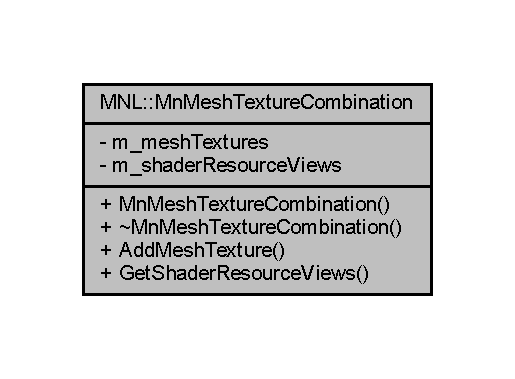
\includegraphics[width=247pt]{class_m_n_l_1_1_mn_mesh_texture_combination__coll__graph}
\end{center}
\end{figure}
\subsection*{Public 멤버 함수}
\begin{DoxyCompactItemize}
\item 
\hyperlink{class_m_n_l_1_1_mn_mesh_texture_combination_ad83519e7ad5c93f11ed7e3a412dafdd8}{Mn\+Mesh\+Texture\+Combination} ()
\item 
\hyperlink{class_m_n_l_1_1_mn_mesh_texture_combination_a651f2956722d41035193c71c27528b52}{$\sim$\+Mn\+Mesh\+Texture\+Combination} ()
\item 
void \hyperlink{class_m_n_l_1_1_mn_mesh_texture_combination_a7f76a68d2b1fb4ac4aad43ff4e70f5e8}{Add\+Mesh\+Texture} (const std\+::shared\+\_\+ptr$<$ \hyperlink{class_m_n_l_1_1_mn_mesh_texture}{Mn\+Mesh\+Texture} $>$ \&sp\+Mesh\+Texture)
\item 
const std\+::vector$<$ \hyperlink{namespace_m_n_l_a93794d93663474ff79c950ed985565aa}{C\+P\+D3\+D\+Shader\+Resource\+View} $>$ \& \hyperlink{class_m_n_l_1_1_mn_mesh_texture_combination_ac9ea285204f40f2808b8697c2738752d}{Get\+Shader\+Resource\+Views} () const
\end{DoxyCompactItemize}
\subsection*{Private 속성}
\begin{DoxyCompactItemize}
\item 
std\+::vector$<$ std\+::shared\+\_\+ptr$<$ \hyperlink{class_m_n_l_1_1_mn_mesh_texture}{Mn\+Mesh\+Texture} $>$ $>$ \hyperlink{class_m_n_l_1_1_mn_mesh_texture_combination_a63aac894ab731ea3ab1024246b561fd7}{m\+\_\+mesh\+Textures}
\item 
std\+::vector$<$ \hyperlink{namespace_m_n_l_a93794d93663474ff79c950ed985565aa}{C\+P\+D3\+D\+Shader\+Resource\+View} $>$ \hyperlink{class_m_n_l_1_1_mn_mesh_texture_combination_a665314c3b4ca74800ecf2d36245cfa0b}{m\+\_\+shader\+Resource\+Views}
\end{DoxyCompactItemize}


\subsection{상세한 설명}


Mn\+Mesh\+Texture\+Combination.\+h 파일의 11 번째 라인에서 정의되었습니다.



\subsection{생성자 \& 소멸자 문서화}
\mbox{\Hypertarget{class_m_n_l_1_1_mn_mesh_texture_combination_ad83519e7ad5c93f11ed7e3a412dafdd8}\label{class_m_n_l_1_1_mn_mesh_texture_combination_ad83519e7ad5c93f11ed7e3a412dafdd8}} 
\index{M\+N\+L\+::\+Mn\+Mesh\+Texture\+Combination@{M\+N\+L\+::\+Mn\+Mesh\+Texture\+Combination}!Mn\+Mesh\+Texture\+Combination@{Mn\+Mesh\+Texture\+Combination}}
\index{Mn\+Mesh\+Texture\+Combination@{Mn\+Mesh\+Texture\+Combination}!M\+N\+L\+::\+Mn\+Mesh\+Texture\+Combination@{M\+N\+L\+::\+Mn\+Mesh\+Texture\+Combination}}
\subsubsection{\texorpdfstring{Mn\+Mesh\+Texture\+Combination()}{MnMeshTextureCombination()}}
{\footnotesize\ttfamily Mn\+Mesh\+Texture\+Combination\+::\+Mn\+Mesh\+Texture\+Combination (\begin{DoxyParamCaption}{ }\end{DoxyParamCaption})}



Mn\+Mesh\+Texture\+Combination.\+cpp 파일의 5 번째 라인에서 정의되었습니다.

\mbox{\Hypertarget{class_m_n_l_1_1_mn_mesh_texture_combination_a651f2956722d41035193c71c27528b52}\label{class_m_n_l_1_1_mn_mesh_texture_combination_a651f2956722d41035193c71c27528b52}} 
\index{M\+N\+L\+::\+Mn\+Mesh\+Texture\+Combination@{M\+N\+L\+::\+Mn\+Mesh\+Texture\+Combination}!````~Mn\+Mesh\+Texture\+Combination@{$\sim$\+Mn\+Mesh\+Texture\+Combination}}
\index{````~Mn\+Mesh\+Texture\+Combination@{$\sim$\+Mn\+Mesh\+Texture\+Combination}!M\+N\+L\+::\+Mn\+Mesh\+Texture\+Combination@{M\+N\+L\+::\+Mn\+Mesh\+Texture\+Combination}}
\subsubsection{\texorpdfstring{$\sim$\+Mn\+Mesh\+Texture\+Combination()}{~MnMeshTextureCombination()}}
{\footnotesize\ttfamily Mn\+Mesh\+Texture\+Combination\+::$\sim$\+Mn\+Mesh\+Texture\+Combination (\begin{DoxyParamCaption}{ }\end{DoxyParamCaption})}



Mn\+Mesh\+Texture\+Combination.\+cpp 파일의 10 번째 라인에서 정의되었습니다.



\subsection{멤버 함수 문서화}
\mbox{\Hypertarget{class_m_n_l_1_1_mn_mesh_texture_combination_a7f76a68d2b1fb4ac4aad43ff4e70f5e8}\label{class_m_n_l_1_1_mn_mesh_texture_combination_a7f76a68d2b1fb4ac4aad43ff4e70f5e8}} 
\index{M\+N\+L\+::\+Mn\+Mesh\+Texture\+Combination@{M\+N\+L\+::\+Mn\+Mesh\+Texture\+Combination}!Add\+Mesh\+Texture@{Add\+Mesh\+Texture}}
\index{Add\+Mesh\+Texture@{Add\+Mesh\+Texture}!M\+N\+L\+::\+Mn\+Mesh\+Texture\+Combination@{M\+N\+L\+::\+Mn\+Mesh\+Texture\+Combination}}
\subsubsection{\texorpdfstring{Add\+Mesh\+Texture()}{AddMeshTexture()}}
{\footnotesize\ttfamily void Mn\+Mesh\+Texture\+Combination\+::\+Add\+Mesh\+Texture (\begin{DoxyParamCaption}\item[{const std\+::shared\+\_\+ptr$<$ \hyperlink{class_m_n_l_1_1_mn_mesh_texture}{Mn\+Mesh\+Texture} $>$ \&}]{sp\+Mesh\+Texture }\end{DoxyParamCaption})}



Mn\+Mesh\+Texture\+Combination.\+cpp 파일의 14 번째 라인에서 정의되었습니다.

\mbox{\Hypertarget{class_m_n_l_1_1_mn_mesh_texture_combination_ac9ea285204f40f2808b8697c2738752d}\label{class_m_n_l_1_1_mn_mesh_texture_combination_ac9ea285204f40f2808b8697c2738752d}} 
\index{M\+N\+L\+::\+Mn\+Mesh\+Texture\+Combination@{M\+N\+L\+::\+Mn\+Mesh\+Texture\+Combination}!Get\+Shader\+Resource\+Views@{Get\+Shader\+Resource\+Views}}
\index{Get\+Shader\+Resource\+Views@{Get\+Shader\+Resource\+Views}!M\+N\+L\+::\+Mn\+Mesh\+Texture\+Combination@{M\+N\+L\+::\+Mn\+Mesh\+Texture\+Combination}}
\subsubsection{\texorpdfstring{Get\+Shader\+Resource\+Views()}{GetShaderResourceViews()}}
{\footnotesize\ttfamily const std\+::vector$<$ \hyperlink{namespace_m_n_l_a93794d93663474ff79c950ed985565aa}{C\+P\+D3\+D\+Shader\+Resource\+View} $>$ \& Mn\+Mesh\+Texture\+Combination\+::\+Get\+Shader\+Resource\+Views (\begin{DoxyParamCaption}{ }\end{DoxyParamCaption}) const}



Mn\+Mesh\+Texture\+Combination.\+cpp 파일의 26 번째 라인에서 정의되었습니다.



\subsection{멤버 데이터 문서화}
\mbox{\Hypertarget{class_m_n_l_1_1_mn_mesh_texture_combination_a63aac894ab731ea3ab1024246b561fd7}\label{class_m_n_l_1_1_mn_mesh_texture_combination_a63aac894ab731ea3ab1024246b561fd7}} 
\index{M\+N\+L\+::\+Mn\+Mesh\+Texture\+Combination@{M\+N\+L\+::\+Mn\+Mesh\+Texture\+Combination}!m\+\_\+mesh\+Textures@{m\+\_\+mesh\+Textures}}
\index{m\+\_\+mesh\+Textures@{m\+\_\+mesh\+Textures}!M\+N\+L\+::\+Mn\+Mesh\+Texture\+Combination@{M\+N\+L\+::\+Mn\+Mesh\+Texture\+Combination}}
\subsubsection{\texorpdfstring{m\+\_\+mesh\+Textures}{m\_meshTextures}}
{\footnotesize\ttfamily std\+::vector$<$std\+::shared\+\_\+ptr$<$\hyperlink{class_m_n_l_1_1_mn_mesh_texture}{Mn\+Mesh\+Texture}$>$ $>$ M\+N\+L\+::\+Mn\+Mesh\+Texture\+Combination\+::m\+\_\+mesh\+Textures\hspace{0.3cm}{\ttfamily [private]}}



Mn\+Mesh\+Texture\+Combination.\+h 파일의 22 번째 라인에서 정의되었습니다.

\mbox{\Hypertarget{class_m_n_l_1_1_mn_mesh_texture_combination_a665314c3b4ca74800ecf2d36245cfa0b}\label{class_m_n_l_1_1_mn_mesh_texture_combination_a665314c3b4ca74800ecf2d36245cfa0b}} 
\index{M\+N\+L\+::\+Mn\+Mesh\+Texture\+Combination@{M\+N\+L\+::\+Mn\+Mesh\+Texture\+Combination}!m\+\_\+shader\+Resource\+Views@{m\+\_\+shader\+Resource\+Views}}
\index{m\+\_\+shader\+Resource\+Views@{m\+\_\+shader\+Resource\+Views}!M\+N\+L\+::\+Mn\+Mesh\+Texture\+Combination@{M\+N\+L\+::\+Mn\+Mesh\+Texture\+Combination}}
\subsubsection{\texorpdfstring{m\+\_\+shader\+Resource\+Views}{m\_shaderResourceViews}}
{\footnotesize\ttfamily std\+::vector$<$\hyperlink{namespace_m_n_l_a93794d93663474ff79c950ed985565aa}{C\+P\+D3\+D\+Shader\+Resource\+View}$>$ M\+N\+L\+::\+Mn\+Mesh\+Texture\+Combination\+::m\+\_\+shader\+Resource\+Views\hspace{0.3cm}{\ttfamily [private]}}



Mn\+Mesh\+Texture\+Combination.\+h 파일의 23 번째 라인에서 정의되었습니다.



이 클래스에 대한 문서화 페이지는 다음의 파일들로부터 생성되었습니다.\+:\begin{DoxyCompactItemize}
\item 
Render/\hyperlink{_mn_mesh_texture_combination_8h}{Mn\+Mesh\+Texture\+Combination.\+h}\item 
Render/\hyperlink{_mn_mesh_texture_combination_8cpp}{Mn\+Mesh\+Texture\+Combination.\+cpp}\end{DoxyCompactItemize}

\hypertarget{class_m_n_l_1_1_mn_mesh_vertex_type}{}\section{M\+NL\+:\+:Mn\+Mesh\+Vertex\+Type 클래스 참조}
\label{class_m_n_l_1_1_mn_mesh_vertex_type}\index{M\+N\+L\+::\+Mn\+Mesh\+Vertex\+Type@{M\+N\+L\+::\+Mn\+Mesh\+Vertex\+Type}}


{\ttfamily \#include $<$Mn\+Mesh\+Vertex\+Type.\+h$>$}



M\+NL\+:\+:Mn\+Mesh\+Vertex\+Type에 대한 상속 다이어그램 \+: \nopagebreak
\begin{figure}[H]
\begin{center}
\leavevmode
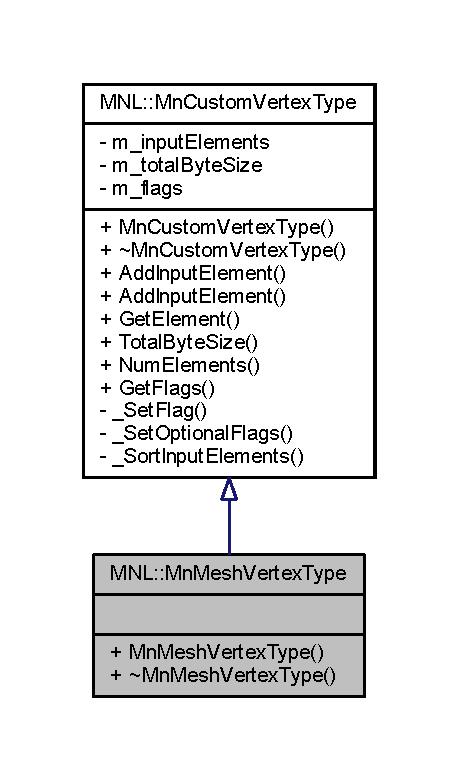
\includegraphics[width=220pt]{class_m_n_l_1_1_mn_mesh_vertex_type__inherit__graph}
\end{center}
\end{figure}


M\+NL\+:\+:Mn\+Mesh\+Vertex\+Type에 대한 협력 다이어그램\+:\nopagebreak
\begin{figure}[H]
\begin{center}
\leavevmode
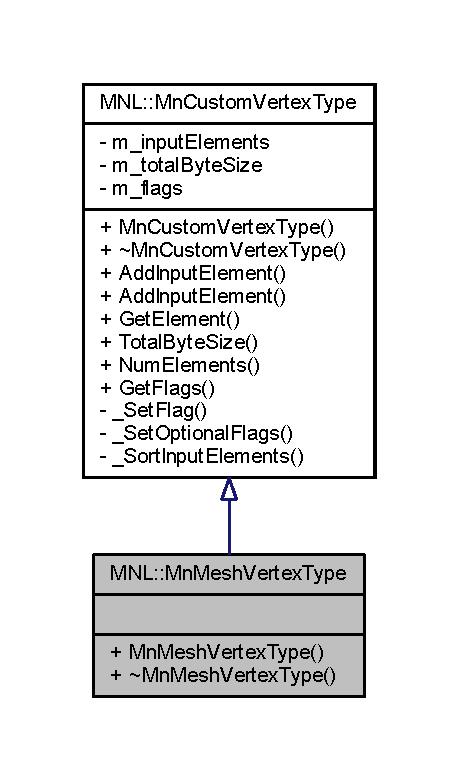
\includegraphics[width=220pt]{class_m_n_l_1_1_mn_mesh_vertex_type__coll__graph}
\end{center}
\end{figure}
\subsection*{Public 멤버 함수}
\begin{DoxyCompactItemize}
\item 
\hyperlink{class_m_n_l_1_1_mn_mesh_vertex_type_a54bd7f4f72e1d8a0d470e4778a262596}{Mn\+Mesh\+Vertex\+Type} ()
\item 
\hyperlink{class_m_n_l_1_1_mn_mesh_vertex_type_aa50f0d7d9e5bd3189fb26e8cdff91472}{$\sim$\+Mn\+Mesh\+Vertex\+Type} ()
\end{DoxyCompactItemize}


\subsection{상세한 설명}


Mn\+Mesh\+Vertex\+Type.\+h 파일의 17 번째 라인에서 정의되었습니다.



\subsection{생성자 \& 소멸자 문서화}
\mbox{\Hypertarget{class_m_n_l_1_1_mn_mesh_vertex_type_a54bd7f4f72e1d8a0d470e4778a262596}\label{class_m_n_l_1_1_mn_mesh_vertex_type_a54bd7f4f72e1d8a0d470e4778a262596}} 
\index{M\+N\+L\+::\+Mn\+Mesh\+Vertex\+Type@{M\+N\+L\+::\+Mn\+Mesh\+Vertex\+Type}!Mn\+Mesh\+Vertex\+Type@{Mn\+Mesh\+Vertex\+Type}}
\index{Mn\+Mesh\+Vertex\+Type@{Mn\+Mesh\+Vertex\+Type}!M\+N\+L\+::\+Mn\+Mesh\+Vertex\+Type@{M\+N\+L\+::\+Mn\+Mesh\+Vertex\+Type}}
\subsubsection{\texorpdfstring{Mn\+Mesh\+Vertex\+Type()}{MnMeshVertexType()}}
{\footnotesize\ttfamily Mn\+Mesh\+Vertex\+Type\+::\+Mn\+Mesh\+Vertex\+Type (\begin{DoxyParamCaption}{ }\end{DoxyParamCaption})}



Mn\+Mesh\+Vertex\+Type.\+cpp 파일의 5 번째 라인에서 정의되었습니다.

\mbox{\Hypertarget{class_m_n_l_1_1_mn_mesh_vertex_type_aa50f0d7d9e5bd3189fb26e8cdff91472}\label{class_m_n_l_1_1_mn_mesh_vertex_type_aa50f0d7d9e5bd3189fb26e8cdff91472}} 
\index{M\+N\+L\+::\+Mn\+Mesh\+Vertex\+Type@{M\+N\+L\+::\+Mn\+Mesh\+Vertex\+Type}!````~Mn\+Mesh\+Vertex\+Type@{$\sim$\+Mn\+Mesh\+Vertex\+Type}}
\index{````~Mn\+Mesh\+Vertex\+Type@{$\sim$\+Mn\+Mesh\+Vertex\+Type}!M\+N\+L\+::\+Mn\+Mesh\+Vertex\+Type@{M\+N\+L\+::\+Mn\+Mesh\+Vertex\+Type}}
\subsubsection{\texorpdfstring{$\sim$\+Mn\+Mesh\+Vertex\+Type()}{~MnMeshVertexType()}}
{\footnotesize\ttfamily Mn\+Mesh\+Vertex\+Type\+::$\sim$\+Mn\+Mesh\+Vertex\+Type (\begin{DoxyParamCaption}{ }\end{DoxyParamCaption})}



Mn\+Mesh\+Vertex\+Type.\+cpp 파일의 13 번째 라인에서 정의되었습니다.



이 클래스에 대한 문서화 페이지는 다음의 파일들로부터 생성되었습니다.\+:\begin{DoxyCompactItemize}
\item 
Render/\hyperlink{_mn_mesh_vertex_type_8h}{Mn\+Mesh\+Vertex\+Type.\+h}\item 
Render/\hyperlink{_mn_mesh_vertex_type_8cpp}{Mn\+Mesh\+Vertex\+Type.\+cpp}\end{DoxyCompactItemize}

\hypertarget{class_m_n_l_1_1_mn_pixel_shader}{}\section{M\+NL\+:\+:Mn\+Pixel\+Shader 클래스 참조}
\label{class_m_n_l_1_1_mn_pixel_shader}\index{M\+N\+L\+::\+Mn\+Pixel\+Shader@{M\+N\+L\+::\+Mn\+Pixel\+Shader}}


{\ttfamily \#include $<$Mn\+Pixel\+Shader.\+h$>$}



M\+NL\+:\+:Mn\+Pixel\+Shader에 대한 협력 다이어그램\+:\nopagebreak
\begin{figure}[H]
\begin{center}
\leavevmode
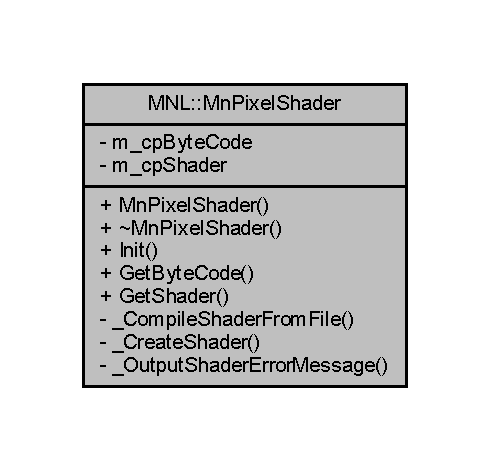
\includegraphics[width=235pt]{class_m_n_l_1_1_mn_pixel_shader__coll__graph}
\end{center}
\end{figure}
\subsection*{Public 멤버 함수}
\begin{DoxyCompactItemize}
\item 
\hyperlink{class_m_n_l_1_1_mn_pixel_shader_a28326df19b17b959ded2b0be89105fcb}{Mn\+Pixel\+Shader} ()
\item 
\hyperlink{class_m_n_l_1_1_mn_pixel_shader_a1cf973996fa4f7cf4155fee3ee32c3b6}{$\sim$\+Mn\+Pixel\+Shader} ()
\item 
H\+R\+E\+S\+U\+LT \hyperlink{class_m_n_l_1_1_mn_pixel_shader_aebcf62590c1e66bd7b9211d227087674}{Init} (\hyperlink{namespace_m_n_l_a1eec210db8f309a4a9ac0d9658784c31}{C\+P\+D3\+D\+Device} cp\+Device, std\+::wstring shader\+File\+Name, std\+::string entry\+Point, std\+::string shader\+Version)
\item 
const \hyperlink{namespace_m_n_l_a3716e3bee60c31fe1b7b5dd5a82db59a}{C\+P\+D3\+D\+Blob} \hyperlink{class_m_n_l_1_1_mn_pixel_shader_a9d25644c65020454a47baa6bed1f7d3e}{Get\+Byte\+Code} () const
\item 
const \hyperlink{namespace_m_n_l_a4d6bd408e6e19137a03728583296f12a}{C\+P\+D3\+D\+Pixel\+Shader} \hyperlink{class_m_n_l_1_1_mn_pixel_shader_a7bb94a0a541152261d7cdce85c9983bf}{Get\+Shader} () const
\end{DoxyCompactItemize}
\subsection*{Private 멤버 함수}
\begin{DoxyCompactItemize}
\item 
\hyperlink{namespace_m_n_l_a3716e3bee60c31fe1b7b5dd5a82db59a}{C\+P\+D3\+D\+Blob} \hyperlink{class_m_n_l_1_1_mn_pixel_shader_a66c1b5bfd8873fefe111e74609066b4c}{\+\_\+\+Compile\+Shader\+From\+File} (const std\+::wstring file\+Name, const std\+::string entry\+Point, const std\+::string shader\+Version)
\item 
H\+R\+E\+S\+U\+LT \hyperlink{class_m_n_l_1_1_mn_pixel_shader_a01cef881b676b0fa699d0cdd0a37b3c9}{\+\_\+\+Create\+Shader} (const \hyperlink{namespace_m_n_l_a1eec210db8f309a4a9ac0d9658784c31}{C\+P\+D3\+D\+Device} cp\+Device, const \hyperlink{namespace_m_n_l_a3716e3bee60c31fe1b7b5dd5a82db59a}{C\+P\+D3\+D\+Blob} cp\+Byte\+Code)
\item 
void \hyperlink{class_m_n_l_1_1_mn_pixel_shader_aa93bd4d048034eefed2b975c6a0bf8eb}{\+\_\+\+Output\+Shader\+Error\+Message} (const \hyperlink{namespace_m_n_l_a3716e3bee60c31fe1b7b5dd5a82db59a}{C\+P\+D3\+D\+Blob} error\+Message)
\end{DoxyCompactItemize}
\subsection*{Private 속성}
\begin{DoxyCompactItemize}
\item 
\hyperlink{namespace_m_n_l_a3716e3bee60c31fe1b7b5dd5a82db59a}{C\+P\+D3\+D\+Blob} \hyperlink{class_m_n_l_1_1_mn_pixel_shader_a427dfc261b2d4ae857025c00063d1e97}{m\+\_\+cp\+Byte\+Code}
\item 
\hyperlink{namespace_m_n_l_a4d6bd408e6e19137a03728583296f12a}{C\+P\+D3\+D\+Pixel\+Shader} \hyperlink{class_m_n_l_1_1_mn_pixel_shader_a93c58b6b8428e3187e9ef53f1c7f3578}{m\+\_\+cp\+Shader}
\end{DoxyCompactItemize}


\subsection{상세한 설명}


Mn\+Pixel\+Shader.\+h 파일의 12 번째 라인에서 정의되었습니다.



\subsection{생성자 \& 소멸자 문서화}
\mbox{\Hypertarget{class_m_n_l_1_1_mn_pixel_shader_a28326df19b17b959ded2b0be89105fcb}\label{class_m_n_l_1_1_mn_pixel_shader_a28326df19b17b959ded2b0be89105fcb}} 
\index{M\+N\+L\+::\+Mn\+Pixel\+Shader@{M\+N\+L\+::\+Mn\+Pixel\+Shader}!Mn\+Pixel\+Shader@{Mn\+Pixel\+Shader}}
\index{Mn\+Pixel\+Shader@{Mn\+Pixel\+Shader}!M\+N\+L\+::\+Mn\+Pixel\+Shader@{M\+N\+L\+::\+Mn\+Pixel\+Shader}}
\subsubsection{\texorpdfstring{Mn\+Pixel\+Shader()}{MnPixelShader()}}
{\footnotesize\ttfamily Mn\+Pixel\+Shader\+::\+Mn\+Pixel\+Shader (\begin{DoxyParamCaption}{ }\end{DoxyParamCaption})}



Mn\+Pixel\+Shader.\+cpp 파일의 8 번째 라인에서 정의되었습니다.

\mbox{\Hypertarget{class_m_n_l_1_1_mn_pixel_shader_a1cf973996fa4f7cf4155fee3ee32c3b6}\label{class_m_n_l_1_1_mn_pixel_shader_a1cf973996fa4f7cf4155fee3ee32c3b6}} 
\index{M\+N\+L\+::\+Mn\+Pixel\+Shader@{M\+N\+L\+::\+Mn\+Pixel\+Shader}!````~Mn\+Pixel\+Shader@{$\sim$\+Mn\+Pixel\+Shader}}
\index{````~Mn\+Pixel\+Shader@{$\sim$\+Mn\+Pixel\+Shader}!M\+N\+L\+::\+Mn\+Pixel\+Shader@{M\+N\+L\+::\+Mn\+Pixel\+Shader}}
\subsubsection{\texorpdfstring{$\sim$\+Mn\+Pixel\+Shader()}{~MnPixelShader()}}
{\footnotesize\ttfamily Mn\+Pixel\+Shader\+::$\sim$\+Mn\+Pixel\+Shader (\begin{DoxyParamCaption}{ }\end{DoxyParamCaption})}



Mn\+Pixel\+Shader.\+cpp 파일의 13 번째 라인에서 정의되었습니다.



\subsection{멤버 함수 문서화}
\mbox{\Hypertarget{class_m_n_l_1_1_mn_pixel_shader_a66c1b5bfd8873fefe111e74609066b4c}\label{class_m_n_l_1_1_mn_pixel_shader_a66c1b5bfd8873fefe111e74609066b4c}} 
\index{M\+N\+L\+::\+Mn\+Pixel\+Shader@{M\+N\+L\+::\+Mn\+Pixel\+Shader}!\+\_\+\+Compile\+Shader\+From\+File@{\+\_\+\+Compile\+Shader\+From\+File}}
\index{\+\_\+\+Compile\+Shader\+From\+File@{\+\_\+\+Compile\+Shader\+From\+File}!M\+N\+L\+::\+Mn\+Pixel\+Shader@{M\+N\+L\+::\+Mn\+Pixel\+Shader}}
\subsubsection{\texorpdfstring{\+\_\+\+Compile\+Shader\+From\+File()}{\_CompileShaderFromFile()}}
{\footnotesize\ttfamily \hyperlink{namespace_m_n_l_a3716e3bee60c31fe1b7b5dd5a82db59a}{C\+P\+D3\+D\+Blob} Mn\+Pixel\+Shader\+::\+\_\+\+Compile\+Shader\+From\+File (\begin{DoxyParamCaption}\item[{const std\+::wstring}]{file\+Name,  }\item[{const std\+::string}]{entry\+Point,  }\item[{const std\+::string}]{shader\+Version }\end{DoxyParamCaption})\hspace{0.3cm}{\ttfamily [private]}}



Mn\+Pixel\+Shader.\+cpp 파일의 46 번째 라인에서 정의되었습니다.

\mbox{\Hypertarget{class_m_n_l_1_1_mn_pixel_shader_a01cef881b676b0fa699d0cdd0a37b3c9}\label{class_m_n_l_1_1_mn_pixel_shader_a01cef881b676b0fa699d0cdd0a37b3c9}} 
\index{M\+N\+L\+::\+Mn\+Pixel\+Shader@{M\+N\+L\+::\+Mn\+Pixel\+Shader}!\+\_\+\+Create\+Shader@{\+\_\+\+Create\+Shader}}
\index{\+\_\+\+Create\+Shader@{\+\_\+\+Create\+Shader}!M\+N\+L\+::\+Mn\+Pixel\+Shader@{M\+N\+L\+::\+Mn\+Pixel\+Shader}}
\subsubsection{\texorpdfstring{\+\_\+\+Create\+Shader()}{\_CreateShader()}}
{\footnotesize\ttfamily H\+R\+E\+S\+U\+LT Mn\+Pixel\+Shader\+::\+\_\+\+Create\+Shader (\begin{DoxyParamCaption}\item[{const \hyperlink{namespace_m_n_l_a1eec210db8f309a4a9ac0d9658784c31}{C\+P\+D3\+D\+Device}}]{cp\+Device,  }\item[{const \hyperlink{namespace_m_n_l_a3716e3bee60c31fe1b7b5dd5a82db59a}{C\+P\+D3\+D\+Blob}}]{cp\+Byte\+Code }\end{DoxyParamCaption})\hspace{0.3cm}{\ttfamily [private]}}



Mn\+Pixel\+Shader.\+cpp 파일의 59 번째 라인에서 정의되었습니다.

\mbox{\Hypertarget{class_m_n_l_1_1_mn_pixel_shader_aa93bd4d048034eefed2b975c6a0bf8eb}\label{class_m_n_l_1_1_mn_pixel_shader_aa93bd4d048034eefed2b975c6a0bf8eb}} 
\index{M\+N\+L\+::\+Mn\+Pixel\+Shader@{M\+N\+L\+::\+Mn\+Pixel\+Shader}!\+\_\+\+Output\+Shader\+Error\+Message@{\+\_\+\+Output\+Shader\+Error\+Message}}
\index{\+\_\+\+Output\+Shader\+Error\+Message@{\+\_\+\+Output\+Shader\+Error\+Message}!M\+N\+L\+::\+Mn\+Pixel\+Shader@{M\+N\+L\+::\+Mn\+Pixel\+Shader}}
\subsubsection{\texorpdfstring{\+\_\+\+Output\+Shader\+Error\+Message()}{\_OutputShaderErrorMessage()}}
{\footnotesize\ttfamily void Mn\+Pixel\+Shader\+::\+\_\+\+Output\+Shader\+Error\+Message (\begin{DoxyParamCaption}\item[{const \hyperlink{namespace_m_n_l_a3716e3bee60c31fe1b7b5dd5a82db59a}{C\+P\+D3\+D\+Blob}}]{error\+Message }\end{DoxyParamCaption})\hspace{0.3cm}{\ttfamily [private]}}



Mn\+Pixel\+Shader.\+cpp 파일의 70 번째 라인에서 정의되었습니다.

\mbox{\Hypertarget{class_m_n_l_1_1_mn_pixel_shader_a9d25644c65020454a47baa6bed1f7d3e}\label{class_m_n_l_1_1_mn_pixel_shader_a9d25644c65020454a47baa6bed1f7d3e}} 
\index{M\+N\+L\+::\+Mn\+Pixel\+Shader@{M\+N\+L\+::\+Mn\+Pixel\+Shader}!Get\+Byte\+Code@{Get\+Byte\+Code}}
\index{Get\+Byte\+Code@{Get\+Byte\+Code}!M\+N\+L\+::\+Mn\+Pixel\+Shader@{M\+N\+L\+::\+Mn\+Pixel\+Shader}}
\subsubsection{\texorpdfstring{Get\+Byte\+Code()}{GetByteCode()}}
{\footnotesize\ttfamily const \hyperlink{namespace_m_n_l_a3716e3bee60c31fe1b7b5dd5a82db59a}{C\+P\+D3\+D\+Blob} Mn\+Pixel\+Shader\+::\+Get\+Byte\+Code (\begin{DoxyParamCaption}{ }\end{DoxyParamCaption}) const}



Mn\+Pixel\+Shader.\+cpp 파일의 36 번째 라인에서 정의되었습니다.

\mbox{\Hypertarget{class_m_n_l_1_1_mn_pixel_shader_a7bb94a0a541152261d7cdce85c9983bf}\label{class_m_n_l_1_1_mn_pixel_shader_a7bb94a0a541152261d7cdce85c9983bf}} 
\index{M\+N\+L\+::\+Mn\+Pixel\+Shader@{M\+N\+L\+::\+Mn\+Pixel\+Shader}!Get\+Shader@{Get\+Shader}}
\index{Get\+Shader@{Get\+Shader}!M\+N\+L\+::\+Mn\+Pixel\+Shader@{M\+N\+L\+::\+Mn\+Pixel\+Shader}}
\subsubsection{\texorpdfstring{Get\+Shader()}{GetShader()}}
{\footnotesize\ttfamily const \hyperlink{namespace_m_n_l_a4d6bd408e6e19137a03728583296f12a}{C\+P\+D3\+D\+Pixel\+Shader} Mn\+Pixel\+Shader\+::\+Get\+Shader (\begin{DoxyParamCaption}{ }\end{DoxyParamCaption}) const}



Mn\+Pixel\+Shader.\+cpp 파일의 40 번째 라인에서 정의되었습니다.

\mbox{\Hypertarget{class_m_n_l_1_1_mn_pixel_shader_aebcf62590c1e66bd7b9211d227087674}\label{class_m_n_l_1_1_mn_pixel_shader_aebcf62590c1e66bd7b9211d227087674}} 
\index{M\+N\+L\+::\+Mn\+Pixel\+Shader@{M\+N\+L\+::\+Mn\+Pixel\+Shader}!Init@{Init}}
\index{Init@{Init}!M\+N\+L\+::\+Mn\+Pixel\+Shader@{M\+N\+L\+::\+Mn\+Pixel\+Shader}}
\subsubsection{\texorpdfstring{Init()}{Init()}}
{\footnotesize\ttfamily H\+R\+E\+S\+U\+LT Mn\+Pixel\+Shader\+::\+Init (\begin{DoxyParamCaption}\item[{\hyperlink{namespace_m_n_l_a1eec210db8f309a4a9ac0d9658784c31}{C\+P\+D3\+D\+Device}}]{cp\+Device,  }\item[{std\+::wstring}]{shader\+File\+Name,  }\item[{std\+::string}]{entry\+Point,  }\item[{std\+::string}]{shader\+Version }\end{DoxyParamCaption})}



Mn\+Pixel\+Shader.\+cpp 파일의 17 번째 라인에서 정의되었습니다.



\subsection{멤버 데이터 문서화}
\mbox{\Hypertarget{class_m_n_l_1_1_mn_pixel_shader_a427dfc261b2d4ae857025c00063d1e97}\label{class_m_n_l_1_1_mn_pixel_shader_a427dfc261b2d4ae857025c00063d1e97}} 
\index{M\+N\+L\+::\+Mn\+Pixel\+Shader@{M\+N\+L\+::\+Mn\+Pixel\+Shader}!m\+\_\+cp\+Byte\+Code@{m\+\_\+cp\+Byte\+Code}}
\index{m\+\_\+cp\+Byte\+Code@{m\+\_\+cp\+Byte\+Code}!M\+N\+L\+::\+Mn\+Pixel\+Shader@{M\+N\+L\+::\+Mn\+Pixel\+Shader}}
\subsubsection{\texorpdfstring{m\+\_\+cp\+Byte\+Code}{m\_cpByteCode}}
{\footnotesize\ttfamily \hyperlink{namespace_m_n_l_a3716e3bee60c31fe1b7b5dd5a82db59a}{C\+P\+D3\+D\+Blob} M\+N\+L\+::\+Mn\+Pixel\+Shader\+::m\+\_\+cp\+Byte\+Code\hspace{0.3cm}{\ttfamily [private]}}



Mn\+Pixel\+Shader.\+h 파일의 32 번째 라인에서 정의되었습니다.

\mbox{\Hypertarget{class_m_n_l_1_1_mn_pixel_shader_a93c58b6b8428e3187e9ef53f1c7f3578}\label{class_m_n_l_1_1_mn_pixel_shader_a93c58b6b8428e3187e9ef53f1c7f3578}} 
\index{M\+N\+L\+::\+Mn\+Pixel\+Shader@{M\+N\+L\+::\+Mn\+Pixel\+Shader}!m\+\_\+cp\+Shader@{m\+\_\+cp\+Shader}}
\index{m\+\_\+cp\+Shader@{m\+\_\+cp\+Shader}!M\+N\+L\+::\+Mn\+Pixel\+Shader@{M\+N\+L\+::\+Mn\+Pixel\+Shader}}
\subsubsection{\texorpdfstring{m\+\_\+cp\+Shader}{m\_cpShader}}
{\footnotesize\ttfamily \hyperlink{namespace_m_n_l_a4d6bd408e6e19137a03728583296f12a}{C\+P\+D3\+D\+Pixel\+Shader} M\+N\+L\+::\+Mn\+Pixel\+Shader\+::m\+\_\+cp\+Shader\hspace{0.3cm}{\ttfamily [private]}}



Mn\+Pixel\+Shader.\+h 파일의 33 번째 라인에서 정의되었습니다.



이 클래스에 대한 문서화 페이지는 다음의 파일들로부터 생성되었습니다.\+:\begin{DoxyCompactItemize}
\item 
Core/\hyperlink{_mn_pixel_shader_8h}{Mn\+Pixel\+Shader.\+h}\item 
Core/\hyperlink{_mn_pixel_shader_8cpp}{Mn\+Pixel\+Shader.\+cpp}\end{DoxyCompactItemize}

\hypertarget{class_m_n_l_1_1_mn_rasterizer_state}{}\section{M\+NL\+:\+:Mn\+Rasterizer\+State 클래스 참조}
\label{class_m_n_l_1_1_mn_rasterizer_state}\index{M\+N\+L\+::\+Mn\+Rasterizer\+State@{M\+N\+L\+::\+Mn\+Rasterizer\+State}}


{\ttfamily \#include $<$Mn\+Rasterizer\+State.\+h$>$}



M\+NL\+:\+:Mn\+Rasterizer\+State에 대한 협력 다이어그램\+:\nopagebreak
\begin{figure}[H]
\begin{center}
\leavevmode
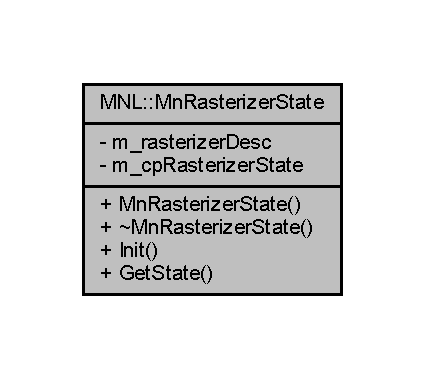
\includegraphics[width=204pt]{class_m_n_l_1_1_mn_rasterizer_state__coll__graph}
\end{center}
\end{figure}
\subsection*{Public 멤버 함수}
\begin{DoxyCompactItemize}
\item 
\hyperlink{class_m_n_l_1_1_mn_rasterizer_state_ac6a6dde00f1bba11b762c0ff21b9598c}{Mn\+Rasterizer\+State} ()
\item 
\hyperlink{class_m_n_l_1_1_mn_rasterizer_state_a414bc5cdc7de69287821dd0ddd08ae52}{$\sim$\+Mn\+Rasterizer\+State} ()
\item 
H\+R\+E\+S\+U\+LT \hyperlink{class_m_n_l_1_1_mn_rasterizer_state_a543c1ca2173258a0af7bbf0cd0e16922}{Init} (\hyperlink{namespace_m_n_l_a1eec210db8f309a4a9ac0d9658784c31}{C\+P\+D3\+D\+Device} cp\+Device, D3\+D11\+\_\+\+F\+I\+L\+L\+\_\+\+M\+O\+DE fill\+Mode, bool is\+C\+CW)
\item 
const \hyperlink{namespace_m_n_l_aa6c2682c64c5b58c458c36bb424f1e56}{C\+P\+D3\+D\+Rasterizer\+State} \hyperlink{class_m_n_l_1_1_mn_rasterizer_state_a91cc6f6e2f11441d31ae75f2c9d65807}{Get\+State} () const
\end{DoxyCompactItemize}
\subsection*{Private 속성}
\begin{DoxyCompactItemize}
\item 
D3\+D11\+\_\+\+R\+A\+S\+T\+E\+R\+I\+Z\+E\+R\+\_\+\+D\+E\+SC \hyperlink{class_m_n_l_1_1_mn_rasterizer_state_a2eeef6c6d928646b13b441999a874ef5}{m\+\_\+rasterizer\+Desc}
\item 
\hyperlink{namespace_m_n_l_aa6c2682c64c5b58c458c36bb424f1e56}{C\+P\+D3\+D\+Rasterizer\+State} \hyperlink{class_m_n_l_1_1_mn_rasterizer_state_a185dd087f95f0e05f6c0cc03cf79b791}{m\+\_\+cp\+Rasterizer\+State}
\end{DoxyCompactItemize}


\subsection{상세한 설명}


Mn\+Rasterizer\+State.\+h 파일의 7 번째 라인에서 정의되었습니다.



\subsection{생성자 \& 소멸자 문서화}
\mbox{\Hypertarget{class_m_n_l_1_1_mn_rasterizer_state_ac6a6dde00f1bba11b762c0ff21b9598c}\label{class_m_n_l_1_1_mn_rasterizer_state_ac6a6dde00f1bba11b762c0ff21b9598c}} 
\index{M\+N\+L\+::\+Mn\+Rasterizer\+State@{M\+N\+L\+::\+Mn\+Rasterizer\+State}!Mn\+Rasterizer\+State@{Mn\+Rasterizer\+State}}
\index{Mn\+Rasterizer\+State@{Mn\+Rasterizer\+State}!M\+N\+L\+::\+Mn\+Rasterizer\+State@{M\+N\+L\+::\+Mn\+Rasterizer\+State}}
\subsubsection{\texorpdfstring{Mn\+Rasterizer\+State()}{MnRasterizerState()}}
{\footnotesize\ttfamily Mn\+Rasterizer\+State\+::\+Mn\+Rasterizer\+State (\begin{DoxyParamCaption}{ }\end{DoxyParamCaption})}



Mn\+Rasterizer\+State.\+cpp 파일의 6 번째 라인에서 정의되었습니다.

\mbox{\Hypertarget{class_m_n_l_1_1_mn_rasterizer_state_a414bc5cdc7de69287821dd0ddd08ae52}\label{class_m_n_l_1_1_mn_rasterizer_state_a414bc5cdc7de69287821dd0ddd08ae52}} 
\index{M\+N\+L\+::\+Mn\+Rasterizer\+State@{M\+N\+L\+::\+Mn\+Rasterizer\+State}!````~Mn\+Rasterizer\+State@{$\sim$\+Mn\+Rasterizer\+State}}
\index{````~Mn\+Rasterizer\+State@{$\sim$\+Mn\+Rasterizer\+State}!M\+N\+L\+::\+Mn\+Rasterizer\+State@{M\+N\+L\+::\+Mn\+Rasterizer\+State}}
\subsubsection{\texorpdfstring{$\sim$\+Mn\+Rasterizer\+State()}{~MnRasterizerState()}}
{\footnotesize\ttfamily Mn\+Rasterizer\+State\+::$\sim$\+Mn\+Rasterizer\+State (\begin{DoxyParamCaption}{ }\end{DoxyParamCaption})}



Mn\+Rasterizer\+State.\+cpp 파일의 12 번째 라인에서 정의되었습니다.



\subsection{멤버 함수 문서화}
\mbox{\Hypertarget{class_m_n_l_1_1_mn_rasterizer_state_a91cc6f6e2f11441d31ae75f2c9d65807}\label{class_m_n_l_1_1_mn_rasterizer_state_a91cc6f6e2f11441d31ae75f2c9d65807}} 
\index{M\+N\+L\+::\+Mn\+Rasterizer\+State@{M\+N\+L\+::\+Mn\+Rasterizer\+State}!Get\+State@{Get\+State}}
\index{Get\+State@{Get\+State}!M\+N\+L\+::\+Mn\+Rasterizer\+State@{M\+N\+L\+::\+Mn\+Rasterizer\+State}}
\subsubsection{\texorpdfstring{Get\+State()}{GetState()}}
{\footnotesize\ttfamily const \hyperlink{namespace_m_n_l_aa6c2682c64c5b58c458c36bb424f1e56}{C\+P\+D3\+D\+Rasterizer\+State} Mn\+Rasterizer\+State\+::\+Get\+State (\begin{DoxyParamCaption}{ }\end{DoxyParamCaption}) const}



Mn\+Rasterizer\+State.\+cpp 파일의 40 번째 라인에서 정의되었습니다.

\mbox{\Hypertarget{class_m_n_l_1_1_mn_rasterizer_state_a543c1ca2173258a0af7bbf0cd0e16922}\label{class_m_n_l_1_1_mn_rasterizer_state_a543c1ca2173258a0af7bbf0cd0e16922}} 
\index{M\+N\+L\+::\+Mn\+Rasterizer\+State@{M\+N\+L\+::\+Mn\+Rasterizer\+State}!Init@{Init}}
\index{Init@{Init}!M\+N\+L\+::\+Mn\+Rasterizer\+State@{M\+N\+L\+::\+Mn\+Rasterizer\+State}}
\subsubsection{\texorpdfstring{Init()}{Init()}}
{\footnotesize\ttfamily H\+R\+E\+S\+U\+LT Mn\+Rasterizer\+State\+::\+Init (\begin{DoxyParamCaption}\item[{\hyperlink{namespace_m_n_l_a1eec210db8f309a4a9ac0d9658784c31}{C\+P\+D3\+D\+Device}}]{cp\+Device,  }\item[{D3\+D11\+\_\+\+F\+I\+L\+L\+\_\+\+M\+O\+DE}]{fill\+Mode,  }\item[{bool}]{is\+C\+CW }\end{DoxyParamCaption})}



Mn\+Rasterizer\+State.\+cpp 파일의 16 번째 라인에서 정의되었습니다.



\subsection{멤버 데이터 문서화}
\mbox{\Hypertarget{class_m_n_l_1_1_mn_rasterizer_state_a185dd087f95f0e05f6c0cc03cf79b791}\label{class_m_n_l_1_1_mn_rasterizer_state_a185dd087f95f0e05f6c0cc03cf79b791}} 
\index{M\+N\+L\+::\+Mn\+Rasterizer\+State@{M\+N\+L\+::\+Mn\+Rasterizer\+State}!m\+\_\+cp\+Rasterizer\+State@{m\+\_\+cp\+Rasterizer\+State}}
\index{m\+\_\+cp\+Rasterizer\+State@{m\+\_\+cp\+Rasterizer\+State}!M\+N\+L\+::\+Mn\+Rasterizer\+State@{M\+N\+L\+::\+Mn\+Rasterizer\+State}}
\subsubsection{\texorpdfstring{m\+\_\+cp\+Rasterizer\+State}{m\_cpRasterizerState}}
{\footnotesize\ttfamily \hyperlink{namespace_m_n_l_aa6c2682c64c5b58c458c36bb424f1e56}{C\+P\+D3\+D\+Rasterizer\+State} M\+N\+L\+::\+Mn\+Rasterizer\+State\+::m\+\_\+cp\+Rasterizer\+State\hspace{0.3cm}{\ttfamily [private]}}



Mn\+Rasterizer\+State.\+h 파일의 17 번째 라인에서 정의되었습니다.

\mbox{\Hypertarget{class_m_n_l_1_1_mn_rasterizer_state_a2eeef6c6d928646b13b441999a874ef5}\label{class_m_n_l_1_1_mn_rasterizer_state_a2eeef6c6d928646b13b441999a874ef5}} 
\index{M\+N\+L\+::\+Mn\+Rasterizer\+State@{M\+N\+L\+::\+Mn\+Rasterizer\+State}!m\+\_\+rasterizer\+Desc@{m\+\_\+rasterizer\+Desc}}
\index{m\+\_\+rasterizer\+Desc@{m\+\_\+rasterizer\+Desc}!M\+N\+L\+::\+Mn\+Rasterizer\+State@{M\+N\+L\+::\+Mn\+Rasterizer\+State}}
\subsubsection{\texorpdfstring{m\+\_\+rasterizer\+Desc}{m\_rasterizerDesc}}
{\footnotesize\ttfamily D3\+D11\+\_\+\+R\+A\+S\+T\+E\+R\+I\+Z\+E\+R\+\_\+\+D\+E\+SC M\+N\+L\+::\+Mn\+Rasterizer\+State\+::m\+\_\+rasterizer\+Desc\hspace{0.3cm}{\ttfamily [private]}}



Mn\+Rasterizer\+State.\+h 파일의 16 번째 라인에서 정의되었습니다.



이 클래스에 대한 문서화 페이지는 다음의 파일들로부터 생성되었습니다.\+:\begin{DoxyCompactItemize}
\item 
Core/\hyperlink{_mn_rasterizer_state_8h}{Mn\+Rasterizer\+State.\+h}\item 
Core/\hyperlink{_mn_rasterizer_state_8cpp}{Mn\+Rasterizer\+State.\+cpp}\end{DoxyCompactItemize}

\hypertarget{class_m_n_l_1_1_mn_render_a_p_i}{}\section{M\+NL\+:\+:Mn\+Render\+A\+PI 클래스 참조}
\label{class_m_n_l_1_1_mn_render_a_p_i}\index{M\+N\+L\+::\+Mn\+Render\+A\+PI@{M\+N\+L\+::\+Mn\+Render\+A\+PI}}


비디오 장치와 상호작용 하는 모든 인터페이스를 지니는 객체  




{\ttfamily \#include $<$Mn\+Render\+A\+P\+I.\+h$>$}



M\+NL\+:\+:Mn\+Render\+A\+P\+I에 대한 협력 다이어그램\+:
\nopagebreak
\begin{figure}[H]
\begin{center}
\leavevmode
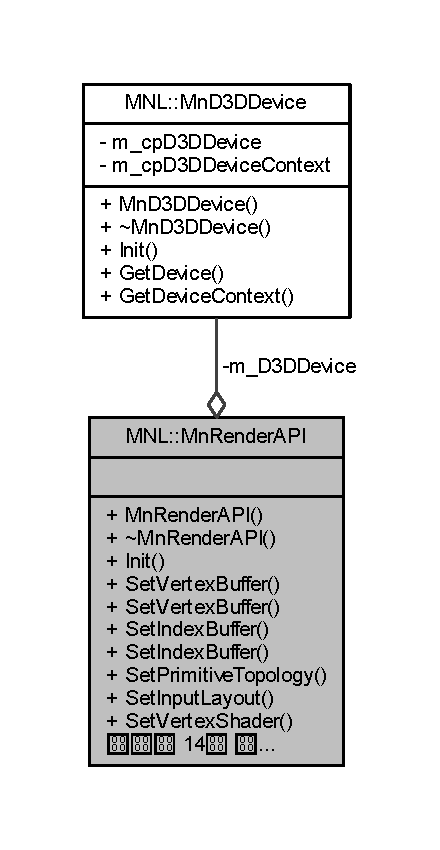
\includegraphics[width=211pt]{class_m_n_l_1_1_mn_render_a_p_i__coll__graph}
\end{center}
\end{figure}
\subsection*{Public 멤버 함수}
\begin{DoxyCompactItemize}
\item 
\hyperlink{class_m_n_l_1_1_mn_render_a_p_i_a3a2932d1caf86bbcfed50b08b1722c74}{Mn\+Render\+A\+PI} ()
\item 
\hyperlink{class_m_n_l_1_1_mn_render_a_p_i_a31ed631cea72b70971ca8917f6010876}{$\sim$\+Mn\+Render\+A\+PI} ()
\item 
H\+R\+E\+S\+U\+LT \hyperlink{class_m_n_l_1_1_mn_render_a_p_i_aef2f0aff53fac021b1c0b3e762d828ab}{Init} (const \hyperlink{class_m_n_l_1_1_mn_hardware}{Mn\+Hardware} \&hardware\+Info, bool use\+Default\+Adapter)
\begin{DoxyCompactList}\small\item\em \hyperlink{class_m_n_l_1_1_mn_hardware}{Mn\+Hardware} 정보를 토대로 Mn\+D3\+D\+Device를 초기화 한다. \end{DoxyCompactList}\item 
void \hyperlink{class_m_n_l_1_1_mn_render_a_p_i_aca919944367349ba7176b83de6954f29}{Set\+Vertex\+Buffer} (const \hyperlink{namespace_m_n_l_aab9c90a8c27ac6410a9cc7cd89efeef1}{C\+P\+D3\+D\+Buffer} \&vertex\+Buffer, U\+I\+NT stride, U\+I\+NT offset)
\begin{DoxyCompactList}\small\item\em 버텍스 버퍼를 그래픽 파이프라인 Input Assembler 단계에 바인드한다. \end{DoxyCompactList}\item 
void \hyperlink{class_m_n_l_1_1_mn_render_a_p_i_a4bcf2ac2d71b25663956493f2cd6c613}{Set\+Vertex\+Buffer} (const \hyperlink{class_m_n_l_1_1_mn_vertex_buffer}{Mn\+Vertex\+Buffer} \&vertex\+Buffer)
\begin{DoxyCompactList}\small\item\em 버텍스 버퍼를 그래픽 파이프라인에 바인드한다. \end{DoxyCompactList}\item 
void \hyperlink{class_m_n_l_1_1_mn_render_a_p_i_a0879f9c1a226921f157e17a308c49840}{Set\+Index\+Buffer} (const \hyperlink{namespace_m_n_l_aab9c90a8c27ac6410a9cc7cd89efeef1}{C\+P\+D3\+D\+Buffer} \&index\+Buffer, D\+X\+G\+I\+\_\+\+F\+O\+R\+M\+AT format)
\begin{DoxyCompactList}\small\item\em 인덱스 버퍼를 그래픽 파이프라인 Input Assembler 단계에 바인드한다. \end{DoxyCompactList}\item 
void \hyperlink{class_m_n_l_1_1_mn_render_a_p_i_a59cab952055a4c763cefe8be9a213b8b}{Set\+Index\+Buffer} (const \hyperlink{class_m_n_l_1_1_mn_index_buffer}{Mn\+Index\+Buffer} \&index\+Buffer)
\begin{DoxyCompactList}\small\item\em 인덱스 버퍼를 그래픽 파이프라인에 바인드한다. \end{DoxyCompactList}\item 
void \hyperlink{class_m_n_l_1_1_mn_render_a_p_i_ade0c9d037798ea2ff940c9eafda403b7}{Set\+Primitive\+Topology} (const D3\+D\+\_\+\+P\+R\+I\+M\+I\+T\+I\+V\+E\+\_\+\+T\+O\+P\+O\+L\+O\+GY \&primitive\+Topology)
\begin{DoxyCompactList}\small\item\em 도형 토폴로지를 그래픽 파이프라인 Input Assembler 단계에 설정한다. \end{DoxyCompactList}\item 
void \hyperlink{class_m_n_l_1_1_mn_render_a_p_i_a1c279cbdd724db75c9b46a235a4eefc3}{Set\+Input\+Layout} (const \hyperlink{namespace_m_n_l_aec7a2a132d6e72492d5feb5926d838dd}{C\+P\+D3\+D\+Input\+Layout} \&cp\+Input\+Layout)
\begin{DoxyCompactList}\small\item\em 인풋 레이아웃을 그래픽 파이프라인 Input Assembler 단계에 설정한다. \end{DoxyCompactList}\item 
void \hyperlink{class_m_n_l_1_1_mn_render_a_p_i_a14436db58cba8d81570cb77f46f6e240}{Set\+Vertex\+Shader} (const \hyperlink{namespace_m_n_l_a8036d713226061c4827b537821fbf79b}{C\+P\+D3\+D\+Vertex\+Shader} \&cp\+Vertex\+Shader)
\begin{DoxyCompactList}\small\item\em 버텍스 셰이더를 그래픽 파이프라인 Vertex Shader 단계에 설정한다. \end{DoxyCompactList}\item 
void \hyperlink{class_m_n_l_1_1_mn_render_a_p_i_a96382bb557949573afd9a1c10eb3e11c}{Set\+Pixel\+Shader} (const \hyperlink{namespace_m_n_l_a4d6bd408e6e19137a03728583296f12a}{C\+P\+D3\+D\+Pixel\+Shader} \&cp\+Pixel\+Shader)
\begin{DoxyCompactList}\small\item\em 픽셀 셰이더를 그래픽 파이프라인 Pixel Shader 단계에 설정한다. \end{DoxyCompactList}\item 
void \hyperlink{class_m_n_l_1_1_mn_render_a_p_i_a52a0598b6ec9617a3019dfa844eab208}{Set\+Constant\+Buffer\+VS} (const \hyperlink{namespace_m_n_l_aab9c90a8c27ac6410a9cc7cd89efeef1}{C\+P\+D3\+D\+Buffer} \&cp\+Constant\+Buffer, U\+I\+NT index)
\begin{DoxyCompactList}\small\item\em 상수 버퍼를 그래픽 파이프라인 Vertex Shader 단계에 설정한다. \end{DoxyCompactList}\item 
void \hyperlink{class_m_n_l_1_1_mn_render_a_p_i_acbefa74f1c90c96711515e9dec3e711f}{Set\+Constant\+Buffer\+PS} (const \hyperlink{namespace_m_n_l_aab9c90a8c27ac6410a9cc7cd89efeef1}{C\+P\+D3\+D\+Buffer} \&cp\+Constant\+Buffer, U\+I\+NT index)
\begin{DoxyCompactList}\small\item\em 상수 버퍼를 그래픽 파이프라인 Pixel Shader 단계에 설정한다. \end{DoxyCompactList}\item 
void \hyperlink{class_m_n_l_1_1_mn_render_a_p_i_a3d3c68e7fe4912e974d89ceeb357793e}{Set\+Sampler\+State} (const \hyperlink{namespace_m_n_l_ae0141196161ecb3d3055523077ca3aa1}{C\+P\+D3\+D\+Sampler\+State} \&cp\+Sampler\+State)
\begin{DoxyCompactList}\small\item\em 샘플러 스테이트를 그래픽 파이프라인 Rasterizer 단계에 설정한다. \end{DoxyCompactList}\item 
void \hyperlink{class_m_n_l_1_1_mn_render_a_p_i_a81810b5ebbfc1fe9cec78ed9e63ab0b0}{Set\+Shader\+Resoure\+View} (const \hyperlink{namespace_m_n_l_a93794d93663474ff79c950ed985565aa}{C\+P\+D3\+D\+Shader\+Resource\+View} \&cp\+Shader\+Resource\+View, U\+I\+NT slot)
\begin{DoxyCompactList}\small\item\em 셰이더 리소스 뷰 (통상 텍스쳐)를 그래픽 파이프라인 Pixel Shader 단계에 설정한다. \end{DoxyCompactList}\item 
void \hyperlink{class_m_n_l_1_1_mn_render_a_p_i_ab9fc7cb2fe9b1dd79b66fe2f169fa46a}{Set\+Render\+Target} (const \hyperlink{namespace_m_n_l_aa08a7c0b5ac9d877dacb57b9306b7b8c}{C\+P\+D3\+D\+Render\+Target\+View} \&cp\+Render\+Target\+View, const \hyperlink{namespace_m_n_l_a12b3c209d76ede855300e637f4192a04}{C\+P\+D3\+D\+Depth\+Stencil\+View} \&cp\+Depth\+Stencil\+View)
\begin{DoxyCompactList}\small\item\em 렌더 타겟 및 뎁스 스텐실 뷰을 그래픽 파이프라인 Output Merger 단계에 설정한다. \end{DoxyCompactList}\item 
void \hyperlink{class_m_n_l_1_1_mn_render_a_p_i_a4780504d046ae21574324f55d9799ea3}{Set\+Depth\+Stencil\+State} (const \hyperlink{namespace_m_n_l_a8209b06065c025e5d6bc2e8ee5925faf}{C\+P\+D3\+D\+Depth\+Stencil\+State} \&cp\+Depth\+Stencil\+State)
\begin{DoxyCompactList}\small\item\em 뎁스 스텐실 스테이트를 그래픽 파이프라인 Output Merger 단계에 설정한다. \end{DoxyCompactList}\item 
void \hyperlink{class_m_n_l_1_1_mn_render_a_p_i_a6bda2a793330625a9afd6e488decd198}{Set\+Rasterizer\+State} (const \hyperlink{namespace_m_n_l_aa6c2682c64c5b58c458c36bb424f1e56}{C\+P\+D3\+D\+Rasterizer\+State} \&cp\+Rasterizer\+State)
\begin{DoxyCompactList}\small\item\em 래스터라이저 스테이트를 그래픽 파이프라인 Rasterizer 단계에 설정한다. \end{DoxyCompactList}\item 
void \hyperlink{class_m_n_l_1_1_mn_render_a_p_i_aec7697c401d411b4fc83268b4d98d9c3}{Set\+Viewport} (const D3\+D11\+\_\+\+V\+I\+E\+W\+P\+O\+RT \&viewport)
\begin{DoxyCompactList}\small\item\em 뷰포트를 그래픽 파이프라인 Rasterizer 단계에 설정한다. \end{DoxyCompactList}\item 
void \hyperlink{class_m_n_l_1_1_mn_render_a_p_i_ac132e08f4e5508d45bdf9e4a9cce0eeb}{Clear\+Render\+Targets} (\hyperlink{namespace_m_n_l_aa08a7c0b5ac9d877dacb57b9306b7b8c}{C\+P\+D3\+D\+Render\+Target\+View} render\+Target\+View, \hyperlink{namespace_m_n_l_a12b3c209d76ede855300e637f4192a04}{C\+P\+D3\+D\+Depth\+Stencil\+View} depth\+Stencil\+View, Direct\+X\+::\+Simple\+Math\+::\+Vector4 color=\{ 0.\+0f, 0.\+0f, 0.\+0f, 0.\+0f \})
\begin{DoxyCompactList}\small\item\em 해당 렌더타겟 뷰와 뎁스 스텐실 뷰를 초기값으로 클리어한다. \end{DoxyCompactList}\item 
void \hyperlink{class_m_n_l_1_1_mn_render_a_p_i_a1d1a5e917ca1719432ce326a101a0cdd}{Draw\+Indexed} (U\+I\+NT index\+Count)
\begin{DoxyCompactList}\small\item\em 그래픽 파이프라인의 드로우 콜. \end{DoxyCompactList}\item 
void \hyperlink{class_m_n_l_1_1_mn_render_a_p_i_ad02c10333d786fdce01af16c265244ea}{Draw\+Indexed} (U\+I\+NT index\+Count, U\+I\+NT index\+Offset, U\+I\+NT vertex\+Base)
\begin{DoxyCompactList}\small\item\em 그래픽 파이프라인의 드로우 콜. \end{DoxyCompactList}\item 
const \hyperlink{namespace_m_n_l_a1eec210db8f309a4a9ac0d9658784c31}{C\+P\+D3\+D\+Device} \hyperlink{class_m_n_l_1_1_mn_render_a_p_i_af7dac77c07b794fc4ff298db83f0d84d}{Get\+D3\+D\+Device} () const
\begin{DoxyCompactList}\small\item\em D3\+D\+Device 인터페이스 \end{DoxyCompactList}\item 
const \hyperlink{namespace_m_n_l_aab3aabb6c9360e44ddc8b0bb563c2107}{C\+P\+D3\+D\+Device\+Context} \hyperlink{class_m_n_l_1_1_mn_render_a_p_i_a945fe3f0b1b917376ea3dbfd051c7fe7}{Get\+D3\+D\+Device\+Context} () const
\begin{DoxyCompactList}\small\item\em D3\+D\+Device\+Context 인터페이스 \end{DoxyCompactList}\end{DoxyCompactItemize}
\subsection*{Private 속성}
\begin{DoxyCompactItemize}
\item 
\hyperlink{class_m_n_l_1_1_mn_d3_d_device}{Mn\+D3\+D\+Device} \hyperlink{class_m_n_l_1_1_mn_render_a_p_i_ac276c60417e41b5cfdb7471da6a6bcdb}{m\+\_\+\+D3\+D\+Device}
\end{DoxyCompactItemize}


\subsection{상세한 설명}
비디오 장치와 상호작용 하는 모든 인터페이스를 지니는 객체 

\begin{DoxyAuthor}{작성자}
Akssus 
\end{DoxyAuthor}
\hypertarget{class_m_n_l_1_1_mn_video_adapter_개요}{}\subsection{개요}\label{class_m_n_l_1_1_mn_video_adapter_개요}
Mn\+Render\+A\+P\+I는 \hyperlink{class_m_n_l_1_1_mn_hardware}{Mn\+Hardware} -\/ \hyperlink{class_m_n_l_1_1_mn_render_a_p_i}{Mn\+Render\+A\+PI} -\/ \hyperlink{class_m_n_l_1_1_mn_render_window}{Mn\+Render\+Window} 로 대표되는 M\+N\+L의 3개의 핵심 클래스 중 하나이다. ~\newline
Mn\+Render\+A\+P\+I는 D3\+D\+Device, D3\+D\+Device\+Context 인터페이스를 통해 비디오 장치와의 상호작용에 관한 모든 인터페이스를 제공한다. ~\newline
Mn\+Render\+A\+P\+I는 그래픽 파이프라인의 대부분의 구간에 접근 가능하며 그래픽 파이프라인의 모든 설정은 Mn\+Render\+A\+P\+I를 통해 설정된다. ~\newline
Mn\+Render\+A\+P\+I는 Draw\+Indexed 드로우 콜을 통해 최종 출력을 실시할 수 있다. 

Mn\+Render\+A\+P\+I.\+h 파일의 26 번째 라인에서 정의되었습니다.



\subsection{생성자 \& 소멸자 문서화}
\mbox{\Hypertarget{class_m_n_l_1_1_mn_render_a_p_i_a3a2932d1caf86bbcfed50b08b1722c74}\label{class_m_n_l_1_1_mn_render_a_p_i_a3a2932d1caf86bbcfed50b08b1722c74}} 
\index{M\+N\+L\+::\+Mn\+Render\+A\+PI@{M\+N\+L\+::\+Mn\+Render\+A\+PI}!Mn\+Render\+A\+PI@{Mn\+Render\+A\+PI}}
\index{Mn\+Render\+A\+PI@{Mn\+Render\+A\+PI}!M\+N\+L\+::\+Mn\+Render\+A\+PI@{M\+N\+L\+::\+Mn\+Render\+A\+PI}}
\subsubsection{\texorpdfstring{Mn\+Render\+A\+P\+I()}{MnRenderAPI()}}
{\footnotesize\ttfamily Mn\+Render\+A\+P\+I\+::\+Mn\+Render\+A\+PI (\begin{DoxyParamCaption}{ }\end{DoxyParamCaption})}



Mn\+Render\+A\+P\+I.\+cpp 파일의 9 번째 라인에서 정의되었습니다.

\mbox{\Hypertarget{class_m_n_l_1_1_mn_render_a_p_i_a31ed631cea72b70971ca8917f6010876}\label{class_m_n_l_1_1_mn_render_a_p_i_a31ed631cea72b70971ca8917f6010876}} 
\index{M\+N\+L\+::\+Mn\+Render\+A\+PI@{M\+N\+L\+::\+Mn\+Render\+A\+PI}!````~Mn\+Render\+A\+PI@{$\sim$\+Mn\+Render\+A\+PI}}
\index{````~Mn\+Render\+A\+PI@{$\sim$\+Mn\+Render\+A\+PI}!M\+N\+L\+::\+Mn\+Render\+A\+PI@{M\+N\+L\+::\+Mn\+Render\+A\+PI}}
\subsubsection{\texorpdfstring{$\sim$\+Mn\+Render\+A\+P\+I()}{~MnRenderAPI()}}
{\footnotesize\ttfamily Mn\+Render\+A\+P\+I\+::$\sim$\+Mn\+Render\+A\+PI (\begin{DoxyParamCaption}{ }\end{DoxyParamCaption})}



Mn\+Render\+A\+P\+I.\+cpp 파일의 14 번째 라인에서 정의되었습니다.



\subsection{멤버 함수 문서화}
\mbox{\Hypertarget{class_m_n_l_1_1_mn_render_a_p_i_ac132e08f4e5508d45bdf9e4a9cce0eeb}\label{class_m_n_l_1_1_mn_render_a_p_i_ac132e08f4e5508d45bdf9e4a9cce0eeb}} 
\index{M\+N\+L\+::\+Mn\+Render\+A\+PI@{M\+N\+L\+::\+Mn\+Render\+A\+PI}!Clear\+Render\+Targets@{Clear\+Render\+Targets}}
\index{Clear\+Render\+Targets@{Clear\+Render\+Targets}!M\+N\+L\+::\+Mn\+Render\+A\+PI@{M\+N\+L\+::\+Mn\+Render\+A\+PI}}
\subsubsection{\texorpdfstring{Clear\+Render\+Targets()}{ClearRenderTargets()}}
{\footnotesize\ttfamily void Mn\+Render\+A\+P\+I\+::\+Clear\+Render\+Targets (\begin{DoxyParamCaption}\item[{\hyperlink{namespace_m_n_l_aa08a7c0b5ac9d877dacb57b9306b7b8c}{C\+P\+D3\+D\+Render\+Target\+View}}]{render\+Target\+View,  }\item[{\hyperlink{namespace_m_n_l_a12b3c209d76ede855300e637f4192a04}{C\+P\+D3\+D\+Depth\+Stencil\+View}}]{depth\+Stencil\+View,  }\item[{Direct\+X\+::\+Simple\+Math\+::\+Vector4}]{color = {\ttfamily \{~0.0f,~0.0f,~0.0f,~0.0f~\}} }\end{DoxyParamCaption})}



해당 렌더타겟 뷰와 뎁스 스텐실 뷰를 초기값으로 클리어한다. 


\begin{DoxyParams}{매개변수}
{\em render\+Target\+View} & 클리어 될 렌더 타겟 뷰. 텍스쳐 혹은 백 버퍼가 될 수 있다. \\
\hline
{\em depth\+Stencil\+View} & 클리어 될 뎁스 스텐실 뷰. 텍스쳐 혹은 백 버퍼가 될 수 있다. 뎁스는 1.\+0f, 스텐실은 0으로 초기화된다. \\
\hline
{\em color} & 렌더 타겟 뷰를 클리어할 색상. 기본값으로 검은색이다. \\
\hline
\end{DoxyParams}


Mn\+Render\+A\+P\+I.\+cpp 파일의 102 번째 라인에서 정의되었습니다.

\mbox{\Hypertarget{class_m_n_l_1_1_mn_render_a_p_i_a1d1a5e917ca1719432ce326a101a0cdd}\label{class_m_n_l_1_1_mn_render_a_p_i_a1d1a5e917ca1719432ce326a101a0cdd}} 
\index{M\+N\+L\+::\+Mn\+Render\+A\+PI@{M\+N\+L\+::\+Mn\+Render\+A\+PI}!Draw\+Indexed@{Draw\+Indexed}}
\index{Draw\+Indexed@{Draw\+Indexed}!M\+N\+L\+::\+Mn\+Render\+A\+PI@{M\+N\+L\+::\+Mn\+Render\+A\+PI}}
\subsubsection{\texorpdfstring{Draw\+Indexed()}{DrawIndexed()}\hspace{0.1cm}{\footnotesize\ttfamily [1/2]}}
{\footnotesize\ttfamily void Mn\+Render\+A\+P\+I\+::\+Draw\+Indexed (\begin{DoxyParamCaption}\item[{U\+I\+NT}]{index\+Count }\end{DoxyParamCaption})}



그래픽 파이프라인의 드로우 콜. 


\begin{DoxyParams}{매개변수}
{\em index\+Count} & 설정된 인덱스 버퍼 내의 인덱스 개수.  인덱스를 참조해 버텍스 버퍼의 메모리로 접근하기 때문에 인덱스의 개수만 알면 된다. 그러므로 버텍스의 개수는 인자로 받지 않는다. \\
\hline
\end{DoxyParams}


Mn\+Render\+A\+P\+I.\+cpp 파일의 108 번째 라인에서 정의되었습니다.

\mbox{\Hypertarget{class_m_n_l_1_1_mn_render_a_p_i_ad02c10333d786fdce01af16c265244ea}\label{class_m_n_l_1_1_mn_render_a_p_i_ad02c10333d786fdce01af16c265244ea}} 
\index{M\+N\+L\+::\+Mn\+Render\+A\+PI@{M\+N\+L\+::\+Mn\+Render\+A\+PI}!Draw\+Indexed@{Draw\+Indexed}}
\index{Draw\+Indexed@{Draw\+Indexed}!M\+N\+L\+::\+Mn\+Render\+A\+PI@{M\+N\+L\+::\+Mn\+Render\+A\+PI}}
\subsubsection{\texorpdfstring{Draw\+Indexed()}{DrawIndexed()}\hspace{0.1cm}{\footnotesize\ttfamily [2/2]}}
{\footnotesize\ttfamily void Mn\+Render\+A\+P\+I\+::\+Draw\+Indexed (\begin{DoxyParamCaption}\item[{U\+I\+NT}]{index\+Count,  }\item[{U\+I\+NT}]{index\+Offset,  }\item[{U\+I\+NT}]{vertex\+Base }\end{DoxyParamCaption})}



그래픽 파이프라인의 드로우 콜. 


\begin{DoxyParams}{매개변수}
{\em index\+Count} & 설정된 인덱스 버퍼 내의 인덱스 개수. \\
\hline
{\em index\+Offset} & 인덱스 버퍼 내의 시작 메모리로부터의 오프셋. \\
\hline
{\em vertex\+Base} & 버텍스 버퍼 내의 시작 메모리로부터의 오프셋.  인덱스를 참조해 버텍스 버퍼의 메모리로 접근하기 때문에 인덱스의 개수만 알면 된다. 그러므로 버텍스의 개수는 인자로 받지 않는다. ~\newline
vertex\+Base는 하나의 버텍스 버퍼 안에 여러 메쉬가 선형으로 붙어 있는 경우 사용된다. ~\newline
예를 들어 vertex\+Base가 10일 경우 인덱스 0은 실제로 인덱스 10이다.~\newline
이는 Mn\+Mesh의 Sub\+Mesh를 구현할 때 사용된다. \\
\hline
\end{DoxyParams}


Mn\+Render\+A\+P\+I.\+cpp 파일의 112 번째 라인에서 정의되었습니다.

\mbox{\Hypertarget{class_m_n_l_1_1_mn_render_a_p_i_af7dac77c07b794fc4ff298db83f0d84d}\label{class_m_n_l_1_1_mn_render_a_p_i_af7dac77c07b794fc4ff298db83f0d84d}} 
\index{M\+N\+L\+::\+Mn\+Render\+A\+PI@{M\+N\+L\+::\+Mn\+Render\+A\+PI}!Get\+D3\+D\+Device@{Get\+D3\+D\+Device}}
\index{Get\+D3\+D\+Device@{Get\+D3\+D\+Device}!M\+N\+L\+::\+Mn\+Render\+A\+PI@{M\+N\+L\+::\+Mn\+Render\+A\+PI}}
\subsubsection{\texorpdfstring{Get\+D3\+D\+Device()}{GetD3DDevice()}}
{\footnotesize\ttfamily const \hyperlink{namespace_m_n_l_a1eec210db8f309a4a9ac0d9658784c31}{C\+P\+D3\+D\+Device} Mn\+Render\+A\+P\+I\+::\+Get\+D3\+D\+Device (\begin{DoxyParamCaption}{ }\end{DoxyParamCaption}) const}



D3\+D\+Device 인터페이스 



Mn\+Render\+A\+P\+I.\+cpp 파일의 121 번째 라인에서 정의되었습니다.

\mbox{\Hypertarget{class_m_n_l_1_1_mn_render_a_p_i_a945fe3f0b1b917376ea3dbfd051c7fe7}\label{class_m_n_l_1_1_mn_render_a_p_i_a945fe3f0b1b917376ea3dbfd051c7fe7}} 
\index{M\+N\+L\+::\+Mn\+Render\+A\+PI@{M\+N\+L\+::\+Mn\+Render\+A\+PI}!Get\+D3\+D\+Device\+Context@{Get\+D3\+D\+Device\+Context}}
\index{Get\+D3\+D\+Device\+Context@{Get\+D3\+D\+Device\+Context}!M\+N\+L\+::\+Mn\+Render\+A\+PI@{M\+N\+L\+::\+Mn\+Render\+A\+PI}}
\subsubsection{\texorpdfstring{Get\+D3\+D\+Device\+Context()}{GetD3DDeviceContext()}}
{\footnotesize\ttfamily const \hyperlink{namespace_m_n_l_aab3aabb6c9360e44ddc8b0bb563c2107}{C\+P\+D3\+D\+Device\+Context} Mn\+Render\+A\+P\+I\+::\+Get\+D3\+D\+Device\+Context (\begin{DoxyParamCaption}{ }\end{DoxyParamCaption}) const}



D3\+D\+Device\+Context 인터페이스 



Mn\+Render\+A\+P\+I.\+cpp 파일의 125 번째 라인에서 정의되었습니다.

\mbox{\Hypertarget{class_m_n_l_1_1_mn_render_a_p_i_aef2f0aff53fac021b1c0b3e762d828ab}\label{class_m_n_l_1_1_mn_render_a_p_i_aef2f0aff53fac021b1c0b3e762d828ab}} 
\index{M\+N\+L\+::\+Mn\+Render\+A\+PI@{M\+N\+L\+::\+Mn\+Render\+A\+PI}!Init@{Init}}
\index{Init@{Init}!M\+N\+L\+::\+Mn\+Render\+A\+PI@{M\+N\+L\+::\+Mn\+Render\+A\+PI}}
\subsubsection{\texorpdfstring{Init()}{Init()}}
{\footnotesize\ttfamily H\+R\+E\+S\+U\+LT Mn\+Render\+A\+P\+I\+::\+Init (\begin{DoxyParamCaption}\item[{const \hyperlink{class_m_n_l_1_1_mn_hardware}{Mn\+Hardware} \&}]{hardware\+Info,  }\item[{bool}]{use\+Default\+Adapter }\end{DoxyParamCaption})}



\hyperlink{class_m_n_l_1_1_mn_hardware}{Mn\+Hardware} 정보를 토대로 Mn\+D3\+D\+Device를 초기화 한다. 


\begin{DoxyParams}{매개변수}
{\em use\+Default\+Adapter} & 디폴트 비디오 어댑터 사용 여부 \\
\hline
\end{DoxyParams}
\begin{DoxyReturn}{반환값}
초기화 성공 여부 
\end{DoxyReturn}
\begin{DoxyWarning}{경고}
현재 use\+Default\+Adapter의 값과 상관없이 디폴트 비디오 어댑터로 초기화 된다. 
\end{DoxyWarning}


Mn\+Render\+A\+P\+I.\+cpp 파일의 18 번째 라인에서 정의되었습니다.

\mbox{\Hypertarget{class_m_n_l_1_1_mn_render_a_p_i_acbefa74f1c90c96711515e9dec3e711f}\label{class_m_n_l_1_1_mn_render_a_p_i_acbefa74f1c90c96711515e9dec3e711f}} 
\index{M\+N\+L\+::\+Mn\+Render\+A\+PI@{M\+N\+L\+::\+Mn\+Render\+A\+PI}!Set\+Constant\+Buffer\+PS@{Set\+Constant\+Buffer\+PS}}
\index{Set\+Constant\+Buffer\+PS@{Set\+Constant\+Buffer\+PS}!M\+N\+L\+::\+Mn\+Render\+A\+PI@{M\+N\+L\+::\+Mn\+Render\+A\+PI}}
\subsubsection{\texorpdfstring{Set\+Constant\+Buffer\+P\+S()}{SetConstantBufferPS()}}
{\footnotesize\ttfamily void Mn\+Render\+A\+P\+I\+::\+Set\+Constant\+Buffer\+PS (\begin{DoxyParamCaption}\item[{const \hyperlink{namespace_m_n_l_aab9c90a8c27ac6410a9cc7cd89efeef1}{C\+P\+D3\+D\+Buffer} \&}]{cp\+Constant\+Buffer,  }\item[{U\+I\+NT}]{index }\end{DoxyParamCaption})}



상수 버퍼를 그래픽 파이프라인 Pixel Shader 단계에 설정한다. 


\begin{DoxyParams}{매개변수}
{\em cp\+Constant\+Buffer} & 상수 버퍼 인터페이스. \hyperlink{class_m_n_l_1_1_mn_constant_buffer}{Mn\+Constant\+Buffer} 객체로부터 얻어올 수 있다. \\
\hline
{\em index} & 상수 버퍼의 레지스터 인덱스. 픽셀 셰이더 내의 register(b\#)으로 바인드 된다. \\
\hline
\end{DoxyParams}


Mn\+Render\+A\+P\+I.\+cpp 파일의 67 번째 라인에서 정의되었습니다.

\mbox{\Hypertarget{class_m_n_l_1_1_mn_render_a_p_i_a52a0598b6ec9617a3019dfa844eab208}\label{class_m_n_l_1_1_mn_render_a_p_i_a52a0598b6ec9617a3019dfa844eab208}} 
\index{M\+N\+L\+::\+Mn\+Render\+A\+PI@{M\+N\+L\+::\+Mn\+Render\+A\+PI}!Set\+Constant\+Buffer\+VS@{Set\+Constant\+Buffer\+VS}}
\index{Set\+Constant\+Buffer\+VS@{Set\+Constant\+Buffer\+VS}!M\+N\+L\+::\+Mn\+Render\+A\+PI@{M\+N\+L\+::\+Mn\+Render\+A\+PI}}
\subsubsection{\texorpdfstring{Set\+Constant\+Buffer\+V\+S()}{SetConstantBufferVS()}}
{\footnotesize\ttfamily void Mn\+Render\+A\+P\+I\+::\+Set\+Constant\+Buffer\+VS (\begin{DoxyParamCaption}\item[{const \hyperlink{namespace_m_n_l_aab9c90a8c27ac6410a9cc7cd89efeef1}{C\+P\+D3\+D\+Buffer} \&}]{cp\+Constant\+Buffer,  }\item[{U\+I\+NT}]{index }\end{DoxyParamCaption})}



상수 버퍼를 그래픽 파이프라인 Vertex Shader 단계에 설정한다. 


\begin{DoxyParams}{매개변수}
{\em cp\+Constant\+Buffer} & 상수 버퍼 인터페이스. \hyperlink{class_m_n_l_1_1_mn_constant_buffer}{Mn\+Constant\+Buffer} 객체로부터 얻어올 수 있다. \\
\hline
{\em index} & 상수 버퍼의 레지스터 인덱스. 버텍스 셰이더 내의 register(b\#)으로 바인드 된다. \\
\hline
\end{DoxyParams}


Mn\+Render\+A\+P\+I.\+cpp 파일의 63 번째 라인에서 정의되었습니다.

\mbox{\Hypertarget{class_m_n_l_1_1_mn_render_a_p_i_a4780504d046ae21574324f55d9799ea3}\label{class_m_n_l_1_1_mn_render_a_p_i_a4780504d046ae21574324f55d9799ea3}} 
\index{M\+N\+L\+::\+Mn\+Render\+A\+PI@{M\+N\+L\+::\+Mn\+Render\+A\+PI}!Set\+Depth\+Stencil\+State@{Set\+Depth\+Stencil\+State}}
\index{Set\+Depth\+Stencil\+State@{Set\+Depth\+Stencil\+State}!M\+N\+L\+::\+Mn\+Render\+A\+PI@{M\+N\+L\+::\+Mn\+Render\+A\+PI}}
\subsubsection{\texorpdfstring{Set\+Depth\+Stencil\+State()}{SetDepthStencilState()}}
{\footnotesize\ttfamily void Mn\+Render\+A\+P\+I\+::\+Set\+Depth\+Stencil\+State (\begin{DoxyParamCaption}\item[{const \hyperlink{namespace_m_n_l_a8209b06065c025e5d6bc2e8ee5925faf}{C\+P\+D3\+D\+Depth\+Stencil\+State} \&}]{cp\+Depth\+Stencil\+State }\end{DoxyParamCaption})}



뎁스 스텐실 스테이트를 그래픽 파이프라인 Output Merger 단계에 설정한다. 


\begin{DoxyParams}{매개변수}
{\em cp\+Depth\+Stencil\+State} & 뎁스 스텐실 스테이트 인터페이스.  뎁스 스텐실 스테이트는 깊이 테스트와 스텐실 테스트 함수를 정의한다. \\
\hline
\end{DoxyParams}


Mn\+Render\+A\+P\+I.\+cpp 파일의 86 번째 라인에서 정의되었습니다.

\mbox{\Hypertarget{class_m_n_l_1_1_mn_render_a_p_i_a0879f9c1a226921f157e17a308c49840}\label{class_m_n_l_1_1_mn_render_a_p_i_a0879f9c1a226921f157e17a308c49840}} 
\index{M\+N\+L\+::\+Mn\+Render\+A\+PI@{M\+N\+L\+::\+Mn\+Render\+A\+PI}!Set\+Index\+Buffer@{Set\+Index\+Buffer}}
\index{Set\+Index\+Buffer@{Set\+Index\+Buffer}!M\+N\+L\+::\+Mn\+Render\+A\+PI@{M\+N\+L\+::\+Mn\+Render\+A\+PI}}
\subsubsection{\texorpdfstring{Set\+Index\+Buffer()}{SetIndexBuffer()}\hspace{0.1cm}{\footnotesize\ttfamily [1/2]}}
{\footnotesize\ttfamily void Mn\+Render\+A\+P\+I\+::\+Set\+Index\+Buffer (\begin{DoxyParamCaption}\item[{const \hyperlink{namespace_m_n_l_aab9c90a8c27ac6410a9cc7cd89efeef1}{C\+P\+D3\+D\+Buffer} \&}]{index\+Buffer,  }\item[{D\+X\+G\+I\+\_\+\+F\+O\+R\+M\+AT}]{format }\end{DoxyParamCaption})}



인덱스 버퍼를 그래픽 파이프라인 Input Assembler 단계에 바인드한다. 


\begin{DoxyParams}{매개변수}
{\em index\+Buffer} & 인덱스 버퍼 인터페이스 \\
\hline
{\em D\+X\+G\+I\+\_\+\+F\+O\+R\+M\+AT} & 인덱스로 사용되는 파일형. 일반적으로 4바이트 U\+I\+N\+T가 사용된다. \\
\hline
\end{DoxyParams}


Mn\+Render\+A\+P\+I.\+cpp 파일의 39 번째 라인에서 정의되었습니다.

\mbox{\Hypertarget{class_m_n_l_1_1_mn_render_a_p_i_a59cab952055a4c763cefe8be9a213b8b}\label{class_m_n_l_1_1_mn_render_a_p_i_a59cab952055a4c763cefe8be9a213b8b}} 
\index{M\+N\+L\+::\+Mn\+Render\+A\+PI@{M\+N\+L\+::\+Mn\+Render\+A\+PI}!Set\+Index\+Buffer@{Set\+Index\+Buffer}}
\index{Set\+Index\+Buffer@{Set\+Index\+Buffer}!M\+N\+L\+::\+Mn\+Render\+A\+PI@{M\+N\+L\+::\+Mn\+Render\+A\+PI}}
\subsubsection{\texorpdfstring{Set\+Index\+Buffer()}{SetIndexBuffer()}\hspace{0.1cm}{\footnotesize\ttfamily [2/2]}}
{\footnotesize\ttfamily void Mn\+Render\+A\+P\+I\+::\+Set\+Index\+Buffer (\begin{DoxyParamCaption}\item[{const \hyperlink{class_m_n_l_1_1_mn_index_buffer}{Mn\+Index\+Buffer} \&}]{index\+Buffer }\end{DoxyParamCaption})}



인덱스 버퍼를 그래픽 파이프라인에 바인드한다. 


\begin{DoxyParams}{매개변수}
{\em index\+Buffer} & 초기화 된 \hyperlink{class_m_n_l_1_1_mn_index_buffer}{Mn\+Index\+Buffer} 객체 \\
\hline
\end{DoxyParams}


Mn\+Render\+A\+P\+I.\+cpp 파일의 43 번째 라인에서 정의되었습니다.

\mbox{\Hypertarget{class_m_n_l_1_1_mn_render_a_p_i_a1c279cbdd724db75c9b46a235a4eefc3}\label{class_m_n_l_1_1_mn_render_a_p_i_a1c279cbdd724db75c9b46a235a4eefc3}} 
\index{M\+N\+L\+::\+Mn\+Render\+A\+PI@{M\+N\+L\+::\+Mn\+Render\+A\+PI}!Set\+Input\+Layout@{Set\+Input\+Layout}}
\index{Set\+Input\+Layout@{Set\+Input\+Layout}!M\+N\+L\+::\+Mn\+Render\+A\+PI@{M\+N\+L\+::\+Mn\+Render\+A\+PI}}
\subsubsection{\texorpdfstring{Set\+Input\+Layout()}{SetInputLayout()}}
{\footnotesize\ttfamily void Mn\+Render\+A\+P\+I\+::\+Set\+Input\+Layout (\begin{DoxyParamCaption}\item[{const \hyperlink{namespace_m_n_l_aec7a2a132d6e72492d5feb5926d838dd}{C\+P\+D3\+D\+Input\+Layout} \&}]{cp\+Input\+Layout }\end{DoxyParamCaption})}



인풋 레이아웃을 그래픽 파이프라인 Input Assembler 단계에 설정한다. 


\begin{DoxyParams}{매개변수}
{\em cp\+Input\+Layout} & 인풋 레이아웃 인터페이스. \hyperlink{class_m_n_l_1_1_mn_input_layout}{Mn\+Input\+Layout} 객체로부터 얻어올 수 있다. \\
\hline
\end{DoxyParams}


Mn\+Render\+A\+P\+I.\+cpp 파일의 51 번째 라인에서 정의되었습니다.

\mbox{\Hypertarget{class_m_n_l_1_1_mn_render_a_p_i_a96382bb557949573afd9a1c10eb3e11c}\label{class_m_n_l_1_1_mn_render_a_p_i_a96382bb557949573afd9a1c10eb3e11c}} 
\index{M\+N\+L\+::\+Mn\+Render\+A\+PI@{M\+N\+L\+::\+Mn\+Render\+A\+PI}!Set\+Pixel\+Shader@{Set\+Pixel\+Shader}}
\index{Set\+Pixel\+Shader@{Set\+Pixel\+Shader}!M\+N\+L\+::\+Mn\+Render\+A\+PI@{M\+N\+L\+::\+Mn\+Render\+A\+PI}}
\subsubsection{\texorpdfstring{Set\+Pixel\+Shader()}{SetPixelShader()}}
{\footnotesize\ttfamily void Mn\+Render\+A\+P\+I\+::\+Set\+Pixel\+Shader (\begin{DoxyParamCaption}\item[{const \hyperlink{namespace_m_n_l_a4d6bd408e6e19137a03728583296f12a}{C\+P\+D3\+D\+Pixel\+Shader} \&}]{cp\+Pixel\+Shader }\end{DoxyParamCaption})}



픽셀 셰이더를 그래픽 파이프라인 Pixel Shader 단계에 설정한다. 


\begin{DoxyParams}{매개변수}
{\em cp\+Pixel\+Shader} & 픽셀 셰이더 인터페이스. \hyperlink{class_m_n_l_1_1_mn_pixel_shader}{Mn\+Pixel\+Shader} 객체로부터 얻어올 수 있다. \\
\hline
\end{DoxyParams}


Mn\+Render\+A\+P\+I.\+cpp 파일의 59 번째 라인에서 정의되었습니다.

\mbox{\Hypertarget{class_m_n_l_1_1_mn_render_a_p_i_ade0c9d037798ea2ff940c9eafda403b7}\label{class_m_n_l_1_1_mn_render_a_p_i_ade0c9d037798ea2ff940c9eafda403b7}} 
\index{M\+N\+L\+::\+Mn\+Render\+A\+PI@{M\+N\+L\+::\+Mn\+Render\+A\+PI}!Set\+Primitive\+Topology@{Set\+Primitive\+Topology}}
\index{Set\+Primitive\+Topology@{Set\+Primitive\+Topology}!M\+N\+L\+::\+Mn\+Render\+A\+PI@{M\+N\+L\+::\+Mn\+Render\+A\+PI}}
\subsubsection{\texorpdfstring{Set\+Primitive\+Topology()}{SetPrimitiveTopology()}}
{\footnotesize\ttfamily void Mn\+Render\+A\+P\+I\+::\+Set\+Primitive\+Topology (\begin{DoxyParamCaption}\item[{const D3\+D\+\_\+\+P\+R\+I\+M\+I\+T\+I\+V\+E\+\_\+\+T\+O\+P\+O\+L\+O\+GY \&}]{primitive\+Topology }\end{DoxyParamCaption})}



도형 토폴로지를 그래픽 파이프라인 Input Assembler 단계에 설정한다. 


\begin{DoxyParams}{매개변수}
{\em primitive\+Topology} & 도형 토폴로지. 통상 D3\+D\+\_\+\+P\+R\+I\+M\+I\+T\+I\+V\+E\+\_\+\+T\+R\+I\+A\+N\+G\+L\+E\+L\+I\+S\+T가 사용된다. \\
\hline
\end{DoxyParams}


Mn\+Render\+A\+P\+I.\+cpp 파일의 47 번째 라인에서 정의되었습니다.

\mbox{\Hypertarget{class_m_n_l_1_1_mn_render_a_p_i_a6bda2a793330625a9afd6e488decd198}\label{class_m_n_l_1_1_mn_render_a_p_i_a6bda2a793330625a9afd6e488decd198}} 
\index{M\+N\+L\+::\+Mn\+Render\+A\+PI@{M\+N\+L\+::\+Mn\+Render\+A\+PI}!Set\+Rasterizer\+State@{Set\+Rasterizer\+State}}
\index{Set\+Rasterizer\+State@{Set\+Rasterizer\+State}!M\+N\+L\+::\+Mn\+Render\+A\+PI@{M\+N\+L\+::\+Mn\+Render\+A\+PI}}
\subsubsection{\texorpdfstring{Set\+Rasterizer\+State()}{SetRasterizerState()}}
{\footnotesize\ttfamily void Mn\+Render\+A\+P\+I\+::\+Set\+Rasterizer\+State (\begin{DoxyParamCaption}\item[{const \hyperlink{namespace_m_n_l_aa6c2682c64c5b58c458c36bb424f1e56}{C\+P\+D3\+D\+Rasterizer\+State} \&}]{cp\+Rasterizer\+State }\end{DoxyParamCaption})}



래스터라이저 스테이트를 그래픽 파이프라인 Rasterizer 단계에 설정한다. 


\begin{DoxyParams}{매개변수}
{\em cp\+Rasterizer\+State} & 래스터라이저 스테이트 인터페이스.  래스터라이저 스테이트는 와이어프레임, 솔리드 필 등 래스터라이즈 방식과 백페이스 컬링 방식을 정의한다. \\
\hline
\end{DoxyParams}


Mn\+Render\+A\+P\+I.\+cpp 파일의 90 번째 라인에서 정의되었습니다.

\mbox{\Hypertarget{class_m_n_l_1_1_mn_render_a_p_i_ab9fc7cb2fe9b1dd79b66fe2f169fa46a}\label{class_m_n_l_1_1_mn_render_a_p_i_ab9fc7cb2fe9b1dd79b66fe2f169fa46a}} 
\index{M\+N\+L\+::\+Mn\+Render\+A\+PI@{M\+N\+L\+::\+Mn\+Render\+A\+PI}!Set\+Render\+Target@{Set\+Render\+Target}}
\index{Set\+Render\+Target@{Set\+Render\+Target}!M\+N\+L\+::\+Mn\+Render\+A\+PI@{M\+N\+L\+::\+Mn\+Render\+A\+PI}}
\subsubsection{\texorpdfstring{Set\+Render\+Target()}{SetRenderTarget()}}
{\footnotesize\ttfamily void Mn\+Render\+A\+P\+I\+::\+Set\+Render\+Target (\begin{DoxyParamCaption}\item[{const \hyperlink{namespace_m_n_l_aa08a7c0b5ac9d877dacb57b9306b7b8c}{C\+P\+D3\+D\+Render\+Target\+View} \&}]{cp\+Render\+Target\+View,  }\item[{const \hyperlink{namespace_m_n_l_a12b3c209d76ede855300e637f4192a04}{C\+P\+D3\+D\+Depth\+Stencil\+View} \&}]{cp\+Depth\+Stencil\+View }\end{DoxyParamCaption})}



렌더 타겟 및 뎁스 스텐실 뷰을 그래픽 파이프라인 Output Merger 단계에 설정한다. 


\begin{DoxyParams}{매개변수}
{\em cp\+Render\+Target\+View} & 렌더타겟 뷰 인터페이스. \\
\hline
{\em cp\+Depth\+Stencil\+View} & 뎁스 스텐실 뷰 인터페이스.  만약 Render-\/to-\/\+Texture 기법을 사용하는 경우 백버퍼와 독립된 렌더타겟 뷰와 뎁스 스텐실 뷰를 생성, 설정해야 한다. \\
\hline
\end{DoxyParams}


Mn\+Render\+A\+P\+I.\+cpp 파일의 79 번째 라인에서 정의되었습니다.

\mbox{\Hypertarget{class_m_n_l_1_1_mn_render_a_p_i_a3d3c68e7fe4912e974d89ceeb357793e}\label{class_m_n_l_1_1_mn_render_a_p_i_a3d3c68e7fe4912e974d89ceeb357793e}} 
\index{M\+N\+L\+::\+Mn\+Render\+A\+PI@{M\+N\+L\+::\+Mn\+Render\+A\+PI}!Set\+Sampler\+State@{Set\+Sampler\+State}}
\index{Set\+Sampler\+State@{Set\+Sampler\+State}!M\+N\+L\+::\+Mn\+Render\+A\+PI@{M\+N\+L\+::\+Mn\+Render\+A\+PI}}
\subsubsection{\texorpdfstring{Set\+Sampler\+State()}{SetSamplerState()}}
{\footnotesize\ttfamily void Mn\+Render\+A\+P\+I\+::\+Set\+Sampler\+State (\begin{DoxyParamCaption}\item[{const \hyperlink{namespace_m_n_l_ae0141196161ecb3d3055523077ca3aa1}{C\+P\+D3\+D\+Sampler\+State} \&}]{cp\+Sampler\+State }\end{DoxyParamCaption})}



샘플러 스테이트를 그래픽 파이프라인 Rasterizer 단계에 설정한다. 


\begin{DoxyParams}{매개변수}
{\em cp\+Sampler\+State} & 샘플러 스테이트 인터페이스. \hyperlink{class_m_n_l_1_1_mn_sampler_state}{Mn\+Sampler\+State} 객체로부터 얻어올 수 있다. \\
\hline
\end{DoxyParams}


Mn\+Render\+A\+P\+I.\+cpp 파일의 71 번째 라인에서 정의되었습니다.

\mbox{\Hypertarget{class_m_n_l_1_1_mn_render_a_p_i_a81810b5ebbfc1fe9cec78ed9e63ab0b0}\label{class_m_n_l_1_1_mn_render_a_p_i_a81810b5ebbfc1fe9cec78ed9e63ab0b0}} 
\index{M\+N\+L\+::\+Mn\+Render\+A\+PI@{M\+N\+L\+::\+Mn\+Render\+A\+PI}!Set\+Shader\+Resoure\+View@{Set\+Shader\+Resoure\+View}}
\index{Set\+Shader\+Resoure\+View@{Set\+Shader\+Resoure\+View}!M\+N\+L\+::\+Mn\+Render\+A\+PI@{M\+N\+L\+::\+Mn\+Render\+A\+PI}}
\subsubsection{\texorpdfstring{Set\+Shader\+Resoure\+View()}{SetShaderResoureView()}}
{\footnotesize\ttfamily void Mn\+Render\+A\+P\+I\+::\+Set\+Shader\+Resoure\+View (\begin{DoxyParamCaption}\item[{const \hyperlink{namespace_m_n_l_a93794d93663474ff79c950ed985565aa}{C\+P\+D3\+D\+Shader\+Resource\+View} \&}]{cp\+Shader\+Resource\+View,  }\item[{U\+I\+NT}]{slot }\end{DoxyParamCaption})}



셰이더 리소스 뷰 (통상 텍스쳐)를 그래픽 파이프라인 Pixel Shader 단계에 설정한다. 


\begin{DoxyParams}{매개변수}
{\em cp\+Shader\+Resource\+View} & 셰이더 리소스 뷰 인터페이스. \\
\hline
{\em slot} & 셰이더 리소스 뷰의 레지스터 슬롯. 픽셀 셰이더 내의 register(t\#)으로 바인드된다. \\
\hline
\end{DoxyParams}


Mn\+Render\+A\+P\+I.\+cpp 파일의 75 번째 라인에서 정의되었습니다.

\mbox{\Hypertarget{class_m_n_l_1_1_mn_render_a_p_i_aca919944367349ba7176b83de6954f29}\label{class_m_n_l_1_1_mn_render_a_p_i_aca919944367349ba7176b83de6954f29}} 
\index{M\+N\+L\+::\+Mn\+Render\+A\+PI@{M\+N\+L\+::\+Mn\+Render\+A\+PI}!Set\+Vertex\+Buffer@{Set\+Vertex\+Buffer}}
\index{Set\+Vertex\+Buffer@{Set\+Vertex\+Buffer}!M\+N\+L\+::\+Mn\+Render\+A\+PI@{M\+N\+L\+::\+Mn\+Render\+A\+PI}}
\subsubsection{\texorpdfstring{Set\+Vertex\+Buffer()}{SetVertexBuffer()}\hspace{0.1cm}{\footnotesize\ttfamily [1/2]}}
{\footnotesize\ttfamily void Mn\+Render\+A\+P\+I\+::\+Set\+Vertex\+Buffer (\begin{DoxyParamCaption}\item[{const \hyperlink{namespace_m_n_l_aab9c90a8c27ac6410a9cc7cd89efeef1}{C\+P\+D3\+D\+Buffer} \&}]{vertex\+Buffer,  }\item[{U\+I\+NT}]{stride,  }\item[{U\+I\+NT}]{offset }\end{DoxyParamCaption})}



버텍스 버퍼를 그래픽 파이프라인 Input Assembler 단계에 바인드한다. 


\begin{DoxyParams}{매개변수}
{\em vertex\+Buffer} & 버텍스 버퍼 인터페이스 \\
\hline
{\em stride} & 버텍스 stride. 버텍스 하나의 byte 크기를 뜻한다. \\
\hline
{\em offset} & 버텍스의 시작 주소로부터의 offset \\
\hline
\end{DoxyParams}


Mn\+Render\+A\+P\+I.\+cpp 파일의 29 번째 라인에서 정의되었습니다.

\mbox{\Hypertarget{class_m_n_l_1_1_mn_render_a_p_i_a4bcf2ac2d71b25663956493f2cd6c613}\label{class_m_n_l_1_1_mn_render_a_p_i_a4bcf2ac2d71b25663956493f2cd6c613}} 
\index{M\+N\+L\+::\+Mn\+Render\+A\+PI@{M\+N\+L\+::\+Mn\+Render\+A\+PI}!Set\+Vertex\+Buffer@{Set\+Vertex\+Buffer}}
\index{Set\+Vertex\+Buffer@{Set\+Vertex\+Buffer}!M\+N\+L\+::\+Mn\+Render\+A\+PI@{M\+N\+L\+::\+Mn\+Render\+A\+PI}}
\subsubsection{\texorpdfstring{Set\+Vertex\+Buffer()}{SetVertexBuffer()}\hspace{0.1cm}{\footnotesize\ttfamily [2/2]}}
{\footnotesize\ttfamily void Mn\+Render\+A\+P\+I\+::\+Set\+Vertex\+Buffer (\begin{DoxyParamCaption}\item[{const \hyperlink{class_m_n_l_1_1_mn_vertex_buffer}{Mn\+Vertex\+Buffer} \&}]{vertex\+Buffer }\end{DoxyParamCaption})}



버텍스 버퍼를 그래픽 파이프라인에 바인드한다. 


\begin{DoxyParams}{매개변수}
{\em vertex\+Buffer} & 초기화 된 \hyperlink{class_m_n_l_1_1_mn_vertex_buffer}{Mn\+Vertex\+Buffer} 객체 \\
\hline
\end{DoxyParams}


Mn\+Render\+A\+P\+I.\+cpp 파일의 33 번째 라인에서 정의되었습니다.

\mbox{\Hypertarget{class_m_n_l_1_1_mn_render_a_p_i_a14436db58cba8d81570cb77f46f6e240}\label{class_m_n_l_1_1_mn_render_a_p_i_a14436db58cba8d81570cb77f46f6e240}} 
\index{M\+N\+L\+::\+Mn\+Render\+A\+PI@{M\+N\+L\+::\+Mn\+Render\+A\+PI}!Set\+Vertex\+Shader@{Set\+Vertex\+Shader}}
\index{Set\+Vertex\+Shader@{Set\+Vertex\+Shader}!M\+N\+L\+::\+Mn\+Render\+A\+PI@{M\+N\+L\+::\+Mn\+Render\+A\+PI}}
\subsubsection{\texorpdfstring{Set\+Vertex\+Shader()}{SetVertexShader()}}
{\footnotesize\ttfamily void Mn\+Render\+A\+P\+I\+::\+Set\+Vertex\+Shader (\begin{DoxyParamCaption}\item[{const \hyperlink{namespace_m_n_l_a8036d713226061c4827b537821fbf79b}{C\+P\+D3\+D\+Vertex\+Shader} \&}]{cp\+Vertex\+Shader }\end{DoxyParamCaption})}



버텍스 셰이더를 그래픽 파이프라인 Vertex Shader 단계에 설정한다. 


\begin{DoxyParams}{매개변수}
{\em cp\+Vertex\+Shader} & 버텍스 셰이더 인터페이스. \hyperlink{class_m_n_l_1_1_mn_vertex_shader}{Mn\+Vertex\+Shader} 객체로부터 얻어올 수 있다. \\
\hline
\end{DoxyParams}


Mn\+Render\+A\+P\+I.\+cpp 파일의 55 번째 라인에서 정의되었습니다.

\mbox{\Hypertarget{class_m_n_l_1_1_mn_render_a_p_i_aec7697c401d411b4fc83268b4d98d9c3}\label{class_m_n_l_1_1_mn_render_a_p_i_aec7697c401d411b4fc83268b4d98d9c3}} 
\index{M\+N\+L\+::\+Mn\+Render\+A\+PI@{M\+N\+L\+::\+Mn\+Render\+A\+PI}!Set\+Viewport@{Set\+Viewport}}
\index{Set\+Viewport@{Set\+Viewport}!M\+N\+L\+::\+Mn\+Render\+A\+PI@{M\+N\+L\+::\+Mn\+Render\+A\+PI}}
\subsubsection{\texorpdfstring{Set\+Viewport()}{SetViewport()}}
{\footnotesize\ttfamily void Mn\+Render\+A\+P\+I\+::\+Set\+Viewport (\begin{DoxyParamCaption}\item[{const D3\+D11\+\_\+\+V\+I\+E\+W\+P\+O\+RT \&}]{viewport }\end{DoxyParamCaption})}



뷰포트를 그래픽 파이프라인 Rasterizer 단계에 설정한다. 


\begin{DoxyParams}{매개변수}
{\em viewport} & 뷰포트 좌표 및 크기가 정의된 뷰포트 객체 \\
\hline
\end{DoxyParams}


Mn\+Render\+A\+P\+I.\+cpp 파일의 95 번째 라인에서 정의되었습니다.



\subsection{멤버 데이터 문서화}
\mbox{\Hypertarget{class_m_n_l_1_1_mn_render_a_p_i_ac276c60417e41b5cfdb7471da6a6bcdb}\label{class_m_n_l_1_1_mn_render_a_p_i_ac276c60417e41b5cfdb7471da6a6bcdb}} 
\index{M\+N\+L\+::\+Mn\+Render\+A\+PI@{M\+N\+L\+::\+Mn\+Render\+A\+PI}!m\+\_\+\+D3\+D\+Device@{m\+\_\+\+D3\+D\+Device}}
\index{m\+\_\+\+D3\+D\+Device@{m\+\_\+\+D3\+D\+Device}!M\+N\+L\+::\+Mn\+Render\+A\+PI@{M\+N\+L\+::\+Mn\+Render\+A\+PI}}
\subsubsection{\texorpdfstring{m\+\_\+\+D3\+D\+Device}{m\_D3DDevice}}
{\footnotesize\ttfamily \hyperlink{class_m_n_l_1_1_mn_d3_d_device}{Mn\+D3\+D\+Device} M\+N\+L\+::\+Mn\+Render\+A\+P\+I\+::m\+\_\+\+D3\+D\+Device\hspace{0.3cm}{\ttfamily [private]}}



Mn\+Render\+A\+P\+I.\+h 파일의 178 번째 라인에서 정의되었습니다.



이 클래스에 대한 문서화 페이지는 다음의 파일들로부터 생성되었습니다.\+:\begin{DoxyCompactItemize}
\item 
Core/\hyperlink{_mn_render_a_p_i_8h}{Mn\+Render\+A\+P\+I.\+h}\item 
Core/\hyperlink{_mn_render_a_p_i_8cpp}{Mn\+Render\+A\+P\+I.\+cpp}\end{DoxyCompactItemize}

\hypertarget{class_m_n_l_1_1_mn_renderer}{}\section{M\+NL\+:\+:Mn\+Renderer 클래스 참조}
\label{class_m_n_l_1_1_mn_renderer}\index{M\+N\+L\+::\+Mn\+Renderer@{M\+N\+L\+::\+Mn\+Renderer}}


{\ttfamily \#include $<$Mn\+Renderer.\+h$>$}



M\+NL\+:\+:Mn\+Renderer에 대한 상속 다이어그램 \+: \nopagebreak
\begin{figure}[H]
\begin{center}
\leavevmode
\includegraphics[width=350pt]{class_m_n_l_1_1_mn_renderer__inherit__graph}
\end{center}
\end{figure}


M\+NL\+:\+:Mn\+Renderer에 대한 협력 다이어그램\+:\nopagebreak
\begin{figure}[H]
\begin{center}
\leavevmode
\includegraphics[width=217pt]{class_m_n_l_1_1_mn_renderer__coll__graph}
\end{center}
\end{figure}
\subsection*{Public 멤버 함수}
\begin{DoxyCompactItemize}
\item 
\hyperlink{class_m_n_l_1_1_mn_renderer_ae1e6f84fd929f28f088dc75925d3652f}{Mn\+Renderer} ()
\item 
\hyperlink{class_m_n_l_1_1_mn_renderer_ae15a007ddf6e9e4da79e5507c23d2b9e}{$\sim$\+Mn\+Renderer} ()
\item 
H\+R\+E\+S\+U\+LT \hyperlink{class_m_n_l_1_1_mn_renderer_a10074dbdae9aad1b7ef6f576638a35a9}{Render\+Mesh} (\hyperlink{class_m_n_l_1_1_mn_render_a_p_i}{Mn\+Render\+A\+PI} \&render\+A\+PI, const std\+::shared\+\_\+ptr$<$ \hyperlink{class_m_n_l_1_1_mn_mesh}{Mn\+Mesh} $>$ model)
\item 
void \hyperlink{class_m_n_l_1_1_mn_renderer_a160d4cfc3c3155c6a2ec83d63916f7c0}{Add\+Shader\+Path\+Instance} (const std\+::shared\+\_\+ptr$<$ \hyperlink{class_m_n_l_1_1_mn_shader_path_instance}{Mn\+Shader\+Path\+Instance} $>$ shader\+Path\+Instance)
\item 
void \hyperlink{class_m_n_l_1_1_mn_renderer_a595c562da7e6319c981aee79122bf568}{Apply\+Shader\+Paths} (\hyperlink{class_m_n_l_1_1_mn_render_a_p_i}{Mn\+Render\+A\+PI} \&render\+A\+PI)
\item 
void \hyperlink{class_m_n_l_1_1_mn_renderer_ae855b8a2e919d2d105f9f5b9a95f5bc6}{Apply\+Constant\+Buffers} (\hyperlink{class_m_n_l_1_1_mn_render_a_p_i}{Mn\+Render\+A\+PI} \&render\+A\+PI)
\item 
U\+I\+NT \hyperlink{class_m_n_l_1_1_mn_renderer_a64e1428dc0d2835c69077c3391841c68}{Get\+Num\+Constant\+Buffers} () const
\item 
const std\+::shared\+\_\+ptr$<$ \hyperlink{class_m_n_l_1_1_mn_constant_buffer}{Mn\+Constant\+Buffer} $>$ \hyperlink{class_m_n_l_1_1_mn_renderer_af2acf082128e501b64645c3cb19fbe32}{Get\+Constant\+Buffer} (U\+I\+NT index) const
\item 
void \hyperlink{class_m_n_l_1_1_mn_renderer_a04dcf13f6f822d2c9c68469a2a0c9ad7}{Update\+Constant\+Buffer} (\hyperlink{class_m_n_l_1_1_mn_render_a_p_i}{Mn\+Render\+A\+PI} \&render\+A\+PI, U\+I\+NT index, const D3\+D11\+\_\+\+S\+U\+B\+R\+E\+S\+O\+U\+R\+C\+E\+\_\+\+D\+A\+TA \&data)
\item 
void \hyperlink{class_m_n_l_1_1_mn_renderer_ae8b45346fcd79ac0f881444ee3b526d6}{Set\+Texture\+Combination} (const std\+::shared\+\_\+ptr$<$ \hyperlink{class_m_n_l_1_1_mn_mesh_texture_combination}{Mn\+Mesh\+Texture\+Combination} $>$ \&sp\+Mesh\+Texture\+Combination)
\item 
void \hyperlink{class_m_n_l_1_1_mn_renderer_a8a1dbdc2abb81d46c786bde59305455b}{Apply\+Textures} (\hyperlink{class_m_n_l_1_1_mn_render_a_p_i}{Mn\+Render\+A\+PI} \&render\+A\+PI)
\end{DoxyCompactItemize}
\subsection*{Protected 멤버 함수}
\begin{DoxyCompactItemize}
\item 
void \hyperlink{class_m_n_l_1_1_mn_renderer_aad18a23f94013284e50162b21950b437}{\+\_\+\+Add\+Constant\+Buffer} (const std\+::shared\+\_\+ptr$<$ \hyperlink{class_m_n_l_1_1_mn_constant_buffer}{Mn\+Constant\+Buffer} $>$ sp\+Constant\+Buffer)
\item 
void \hyperlink{class_m_n_l_1_1_mn_renderer_a4e99adeded808fdde2e0b79d2719c03e}{\+\_\+\+Bind\+Constant\+Buffers} (\hyperlink{class_m_n_l_1_1_mn_render_a_p_i}{Mn\+Render\+A\+PI} \&render\+A\+PI)
\item 
void \hyperlink{class_m_n_l_1_1_mn_renderer_a5306058d3813bdf14af2a42b0df96eef}{\+\_\+\+Clear\+Constant\+Buffers} ()
\end{DoxyCompactItemize}
\subsection*{Private 속성}
\begin{DoxyCompactItemize}
\item 
std\+::vector$<$ std\+::shared\+\_\+ptr$<$ \hyperlink{class_m_n_l_1_1_mn_shader_path_instance}{Mn\+Shader\+Path\+Instance} $>$ $>$ \hyperlink{class_m_n_l_1_1_mn_renderer_ab2782a8dee330b39de532974dcf50929}{m\+\_\+shader\+Paths}
\item 
std\+::vector$<$ std\+::shared\+\_\+ptr$<$ \hyperlink{class_m_n_l_1_1_mn_constant_buffer}{Mn\+Constant\+Buffer} $>$ $>$ \hyperlink{class_m_n_l_1_1_mn_renderer_a3d4ca55924319da2153714ed6a1f59d9}{m\+\_\+constant\+Buffers}
\item 
std\+::shared\+\_\+ptr$<$ \hyperlink{class_m_n_l_1_1_mn_mesh_texture_combination}{Mn\+Mesh\+Texture\+Combination} $>$ \hyperlink{class_m_n_l_1_1_mn_renderer_a477f74d577f3ed816965d62f8c5d3f1d}{m\+\_\+sp\+Texture\+Combination}
\item 
std\+::map$<$ U\+I\+NT, U\+I\+NT $>$ \hyperlink{class_m_n_l_1_1_mn_renderer_a3d4ccdbf5591d5012c7aec46cf4b9ee7}{m\+\_\+map\+Index\+To\+Slot}
\item 
U\+I\+NT \hyperlink{class_m_n_l_1_1_mn_renderer_a167618f49362aa7abf93b413ebc82536}{m\+\_\+num\+Vs\+Constant\+Buffers}
\item 
U\+I\+NT \hyperlink{class_m_n_l_1_1_mn_renderer_a9715af5cd993d8b9a458663c9f2e1a40}{m\+\_\+num\+Ps\+Constant\+Buffers}
\end{DoxyCompactItemize}


\subsection{상세한 설명}


Mn\+Renderer.\+h 파일의 17 번째 라인에서 정의되었습니다.



\subsection{생성자 \& 소멸자 문서화}
\mbox{\Hypertarget{class_m_n_l_1_1_mn_renderer_ae1e6f84fd929f28f088dc75925d3652f}\label{class_m_n_l_1_1_mn_renderer_ae1e6f84fd929f28f088dc75925d3652f}} 
\index{M\+N\+L\+::\+Mn\+Renderer@{M\+N\+L\+::\+Mn\+Renderer}!Mn\+Renderer@{Mn\+Renderer}}
\index{Mn\+Renderer@{Mn\+Renderer}!M\+N\+L\+::\+Mn\+Renderer@{M\+N\+L\+::\+Mn\+Renderer}}
\subsubsection{\texorpdfstring{Mn\+Renderer()}{MnRenderer()}}
{\footnotesize\ttfamily Mn\+Renderer\+::\+Mn\+Renderer (\begin{DoxyParamCaption}{ }\end{DoxyParamCaption})}



Mn\+Renderer.\+cpp 파일의 5 번째 라인에서 정의되었습니다.

\mbox{\Hypertarget{class_m_n_l_1_1_mn_renderer_ae15a007ddf6e9e4da79e5507c23d2b9e}\label{class_m_n_l_1_1_mn_renderer_ae15a007ddf6e9e4da79e5507c23d2b9e}} 
\index{M\+N\+L\+::\+Mn\+Renderer@{M\+N\+L\+::\+Mn\+Renderer}!````~Mn\+Renderer@{$\sim$\+Mn\+Renderer}}
\index{````~Mn\+Renderer@{$\sim$\+Mn\+Renderer}!M\+N\+L\+::\+Mn\+Renderer@{M\+N\+L\+::\+Mn\+Renderer}}
\subsubsection{\texorpdfstring{$\sim$\+Mn\+Renderer()}{~MnRenderer()}}
{\footnotesize\ttfamily Mn\+Renderer\+::$\sim$\+Mn\+Renderer (\begin{DoxyParamCaption}{ }\end{DoxyParamCaption})}



Mn\+Renderer.\+cpp 파일의 10 번째 라인에서 정의되었습니다.



\subsection{멤버 함수 문서화}
\mbox{\Hypertarget{class_m_n_l_1_1_mn_renderer_aad18a23f94013284e50162b21950b437}\label{class_m_n_l_1_1_mn_renderer_aad18a23f94013284e50162b21950b437}} 
\index{M\+N\+L\+::\+Mn\+Renderer@{M\+N\+L\+::\+Mn\+Renderer}!\+\_\+\+Add\+Constant\+Buffer@{\+\_\+\+Add\+Constant\+Buffer}}
\index{\+\_\+\+Add\+Constant\+Buffer@{\+\_\+\+Add\+Constant\+Buffer}!M\+N\+L\+::\+Mn\+Renderer@{M\+N\+L\+::\+Mn\+Renderer}}
\subsubsection{\texorpdfstring{\+\_\+\+Add\+Constant\+Buffer()}{\_AddConstantBuffer()}}
{\footnotesize\ttfamily void Mn\+Renderer\+::\+\_\+\+Add\+Constant\+Buffer (\begin{DoxyParamCaption}\item[{const std\+::shared\+\_\+ptr$<$ \hyperlink{class_m_n_l_1_1_mn_constant_buffer}{Mn\+Constant\+Buffer} $>$}]{sp\+Constant\+Buffer }\end{DoxyParamCaption})\hspace{0.3cm}{\ttfamily [protected]}}



Mn\+Renderer.\+cpp 파일의 46 번째 라인에서 정의되었습니다.

\mbox{\Hypertarget{class_m_n_l_1_1_mn_renderer_a4e99adeded808fdde2e0b79d2719c03e}\label{class_m_n_l_1_1_mn_renderer_a4e99adeded808fdde2e0b79d2719c03e}} 
\index{M\+N\+L\+::\+Mn\+Renderer@{M\+N\+L\+::\+Mn\+Renderer}!\+\_\+\+Bind\+Constant\+Buffers@{\+\_\+\+Bind\+Constant\+Buffers}}
\index{\+\_\+\+Bind\+Constant\+Buffers@{\+\_\+\+Bind\+Constant\+Buffers}!M\+N\+L\+::\+Mn\+Renderer@{M\+N\+L\+::\+Mn\+Renderer}}
\subsubsection{\texorpdfstring{\+\_\+\+Bind\+Constant\+Buffers()}{\_BindConstantBuffers()}}
{\footnotesize\ttfamily void Mn\+Renderer\+::\+\_\+\+Bind\+Constant\+Buffers (\begin{DoxyParamCaption}\item[{\hyperlink{class_m_n_l_1_1_mn_render_a_p_i}{Mn\+Render\+A\+PI} \&}]{render\+A\+PI }\end{DoxyParamCaption})\hspace{0.3cm}{\ttfamily [protected]}}



Mn\+Renderer.\+cpp 파일의 91 번째 라인에서 정의되었습니다.

\mbox{\Hypertarget{class_m_n_l_1_1_mn_renderer_a5306058d3813bdf14af2a42b0df96eef}\label{class_m_n_l_1_1_mn_renderer_a5306058d3813bdf14af2a42b0df96eef}} 
\index{M\+N\+L\+::\+Mn\+Renderer@{M\+N\+L\+::\+Mn\+Renderer}!\+\_\+\+Clear\+Constant\+Buffers@{\+\_\+\+Clear\+Constant\+Buffers}}
\index{\+\_\+\+Clear\+Constant\+Buffers@{\+\_\+\+Clear\+Constant\+Buffers}!M\+N\+L\+::\+Mn\+Renderer@{M\+N\+L\+::\+Mn\+Renderer}}
\subsubsection{\texorpdfstring{\+\_\+\+Clear\+Constant\+Buffers()}{\_ClearConstantBuffers()}}
{\footnotesize\ttfamily void Mn\+Renderer\+::\+\_\+\+Clear\+Constant\+Buffers (\begin{DoxyParamCaption}{ }\end{DoxyParamCaption})\hspace{0.3cm}{\ttfamily [protected]}}



Mn\+Renderer.\+cpp 파일의 109 번째 라인에서 정의되었습니다.

\mbox{\Hypertarget{class_m_n_l_1_1_mn_renderer_a160d4cfc3c3155c6a2ec83d63916f7c0}\label{class_m_n_l_1_1_mn_renderer_a160d4cfc3c3155c6a2ec83d63916f7c0}} 
\index{M\+N\+L\+::\+Mn\+Renderer@{M\+N\+L\+::\+Mn\+Renderer}!Add\+Shader\+Path\+Instance@{Add\+Shader\+Path\+Instance}}
\index{Add\+Shader\+Path\+Instance@{Add\+Shader\+Path\+Instance}!M\+N\+L\+::\+Mn\+Renderer@{M\+N\+L\+::\+Mn\+Renderer}}
\subsubsection{\texorpdfstring{Add\+Shader\+Path\+Instance()}{AddShaderPathInstance()}}
{\footnotesize\ttfamily void Mn\+Renderer\+::\+Add\+Shader\+Path\+Instance (\begin{DoxyParamCaption}\item[{const std\+::shared\+\_\+ptr$<$ \hyperlink{class_m_n_l_1_1_mn_shader_path_instance}{Mn\+Shader\+Path\+Instance} $>$}]{shader\+Path\+Instance }\end{DoxyParamCaption})}



Mn\+Renderer.\+cpp 파일의 31 번째 라인에서 정의되었습니다.

\mbox{\Hypertarget{class_m_n_l_1_1_mn_renderer_ae855b8a2e919d2d105f9f5b9a95f5bc6}\label{class_m_n_l_1_1_mn_renderer_ae855b8a2e919d2d105f9f5b9a95f5bc6}} 
\index{M\+N\+L\+::\+Mn\+Renderer@{M\+N\+L\+::\+Mn\+Renderer}!Apply\+Constant\+Buffers@{Apply\+Constant\+Buffers}}
\index{Apply\+Constant\+Buffers@{Apply\+Constant\+Buffers}!M\+N\+L\+::\+Mn\+Renderer@{M\+N\+L\+::\+Mn\+Renderer}}
\subsubsection{\texorpdfstring{Apply\+Constant\+Buffers()}{ApplyConstantBuffers()}}
{\footnotesize\ttfamily void Mn\+Renderer\+::\+Apply\+Constant\+Buffers (\begin{DoxyParamCaption}\item[{\hyperlink{class_m_n_l_1_1_mn_render_a_p_i}{Mn\+Render\+A\+PI} \&}]{render\+A\+PI }\end{DoxyParamCaption})}



Mn\+Renderer.\+cpp 파일의 61 번째 라인에서 정의되었습니다.

\mbox{\Hypertarget{class_m_n_l_1_1_mn_renderer_a595c562da7e6319c981aee79122bf568}\label{class_m_n_l_1_1_mn_renderer_a595c562da7e6319c981aee79122bf568}} 
\index{M\+N\+L\+::\+Mn\+Renderer@{M\+N\+L\+::\+Mn\+Renderer}!Apply\+Shader\+Paths@{Apply\+Shader\+Paths}}
\index{Apply\+Shader\+Paths@{Apply\+Shader\+Paths}!M\+N\+L\+::\+Mn\+Renderer@{M\+N\+L\+::\+Mn\+Renderer}}
\subsubsection{\texorpdfstring{Apply\+Shader\+Paths()}{ApplyShaderPaths()}}
{\footnotesize\ttfamily void Mn\+Renderer\+::\+Apply\+Shader\+Paths (\begin{DoxyParamCaption}\item[{\hyperlink{class_m_n_l_1_1_mn_render_a_p_i}{Mn\+Render\+A\+PI} \&}]{render\+A\+PI }\end{DoxyParamCaption})}



Mn\+Renderer.\+cpp 파일의 35 번째 라인에서 정의되었습니다.

\mbox{\Hypertarget{class_m_n_l_1_1_mn_renderer_a8a1dbdc2abb81d46c786bde59305455b}\label{class_m_n_l_1_1_mn_renderer_a8a1dbdc2abb81d46c786bde59305455b}} 
\index{M\+N\+L\+::\+Mn\+Renderer@{M\+N\+L\+::\+Mn\+Renderer}!Apply\+Textures@{Apply\+Textures}}
\index{Apply\+Textures@{Apply\+Textures}!M\+N\+L\+::\+Mn\+Renderer@{M\+N\+L\+::\+Mn\+Renderer}}
\subsubsection{\texorpdfstring{Apply\+Textures()}{ApplyTextures()}}
{\footnotesize\ttfamily void Mn\+Renderer\+::\+Apply\+Textures (\begin{DoxyParamCaption}\item[{\hyperlink{class_m_n_l_1_1_mn_render_a_p_i}{Mn\+Render\+A\+PI} \&}]{render\+A\+PI }\end{DoxyParamCaption})}



Mn\+Renderer.\+cpp 파일의 82 번째 라인에서 정의되었습니다.

\mbox{\Hypertarget{class_m_n_l_1_1_mn_renderer_af2acf082128e501b64645c3cb19fbe32}\label{class_m_n_l_1_1_mn_renderer_af2acf082128e501b64645c3cb19fbe32}} 
\index{M\+N\+L\+::\+Mn\+Renderer@{M\+N\+L\+::\+Mn\+Renderer}!Get\+Constant\+Buffer@{Get\+Constant\+Buffer}}
\index{Get\+Constant\+Buffer@{Get\+Constant\+Buffer}!M\+N\+L\+::\+Mn\+Renderer@{M\+N\+L\+::\+Mn\+Renderer}}
\subsubsection{\texorpdfstring{Get\+Constant\+Buffer()}{GetConstantBuffer()}}
{\footnotesize\ttfamily const std\+::shared\+\_\+ptr$<$ \hyperlink{class_m_n_l_1_1_mn_constant_buffer}{Mn\+Constant\+Buffer} $>$ Mn\+Renderer\+::\+Get\+Constant\+Buffer (\begin{DoxyParamCaption}\item[{U\+I\+NT}]{index }\end{DoxyParamCaption}) const}



Mn\+Renderer.\+cpp 파일의 70 번째 라인에서 정의되었습니다.

\mbox{\Hypertarget{class_m_n_l_1_1_mn_renderer_a64e1428dc0d2835c69077c3391841c68}\label{class_m_n_l_1_1_mn_renderer_a64e1428dc0d2835c69077c3391841c68}} 
\index{M\+N\+L\+::\+Mn\+Renderer@{M\+N\+L\+::\+Mn\+Renderer}!Get\+Num\+Constant\+Buffers@{Get\+Num\+Constant\+Buffers}}
\index{Get\+Num\+Constant\+Buffers@{Get\+Num\+Constant\+Buffers}!M\+N\+L\+::\+Mn\+Renderer@{M\+N\+L\+::\+Mn\+Renderer}}
\subsubsection{\texorpdfstring{Get\+Num\+Constant\+Buffers()}{GetNumConstantBuffers()}}
{\footnotesize\ttfamily U\+I\+NT Mn\+Renderer\+::\+Get\+Num\+Constant\+Buffers (\begin{DoxyParamCaption}{ }\end{DoxyParamCaption}) const}



Mn\+Renderer.\+cpp 파일의 66 번째 라인에서 정의되었습니다.

\mbox{\Hypertarget{class_m_n_l_1_1_mn_renderer_a10074dbdae9aad1b7ef6f576638a35a9}\label{class_m_n_l_1_1_mn_renderer_a10074dbdae9aad1b7ef6f576638a35a9}} 
\index{M\+N\+L\+::\+Mn\+Renderer@{M\+N\+L\+::\+Mn\+Renderer}!Render\+Mesh@{Render\+Mesh}}
\index{Render\+Mesh@{Render\+Mesh}!M\+N\+L\+::\+Mn\+Renderer@{M\+N\+L\+::\+Mn\+Renderer}}
\subsubsection{\texorpdfstring{Render\+Mesh()}{RenderMesh()}}
{\footnotesize\ttfamily H\+R\+E\+S\+U\+LT Mn\+Renderer\+::\+Render\+Mesh (\begin{DoxyParamCaption}\item[{\hyperlink{class_m_n_l_1_1_mn_render_a_p_i}{Mn\+Render\+A\+PI} \&}]{render\+A\+PI,  }\item[{const std\+::shared\+\_\+ptr$<$ \hyperlink{class_m_n_l_1_1_mn_mesh}{Mn\+Mesh} $>$}]{model }\end{DoxyParamCaption})}



Mn\+Renderer.\+cpp 파일의 14 번째 라인에서 정의되었습니다.

\mbox{\Hypertarget{class_m_n_l_1_1_mn_renderer_ae8b45346fcd79ac0f881444ee3b526d6}\label{class_m_n_l_1_1_mn_renderer_ae8b45346fcd79ac0f881444ee3b526d6}} 
\index{M\+N\+L\+::\+Mn\+Renderer@{M\+N\+L\+::\+Mn\+Renderer}!Set\+Texture\+Combination@{Set\+Texture\+Combination}}
\index{Set\+Texture\+Combination@{Set\+Texture\+Combination}!M\+N\+L\+::\+Mn\+Renderer@{M\+N\+L\+::\+Mn\+Renderer}}
\subsubsection{\texorpdfstring{Set\+Texture\+Combination()}{SetTextureCombination()}}
{\footnotesize\ttfamily void Mn\+Renderer\+::\+Set\+Texture\+Combination (\begin{DoxyParamCaption}\item[{const std\+::shared\+\_\+ptr$<$ \hyperlink{class_m_n_l_1_1_mn_mesh_texture_combination}{Mn\+Mesh\+Texture\+Combination} $>$ \&}]{sp\+Mesh\+Texture\+Combination }\end{DoxyParamCaption})}



Mn\+Renderer.\+cpp 파일의 78 번째 라인에서 정의되었습니다.

\mbox{\Hypertarget{class_m_n_l_1_1_mn_renderer_a04dcf13f6f822d2c9c68469a2a0c9ad7}\label{class_m_n_l_1_1_mn_renderer_a04dcf13f6f822d2c9c68469a2a0c9ad7}} 
\index{M\+N\+L\+::\+Mn\+Renderer@{M\+N\+L\+::\+Mn\+Renderer}!Update\+Constant\+Buffer@{Update\+Constant\+Buffer}}
\index{Update\+Constant\+Buffer@{Update\+Constant\+Buffer}!M\+N\+L\+::\+Mn\+Renderer@{M\+N\+L\+::\+Mn\+Renderer}}
\subsubsection{\texorpdfstring{Update\+Constant\+Buffer()}{UpdateConstantBuffer()}}
{\footnotesize\ttfamily void Mn\+Renderer\+::\+Update\+Constant\+Buffer (\begin{DoxyParamCaption}\item[{\hyperlink{class_m_n_l_1_1_mn_render_a_p_i}{Mn\+Render\+A\+PI} \&}]{render\+A\+PI,  }\item[{U\+I\+NT}]{index,  }\item[{const D3\+D11\+\_\+\+S\+U\+B\+R\+E\+S\+O\+U\+R\+C\+E\+\_\+\+D\+A\+TA \&}]{data }\end{DoxyParamCaption})}



Mn\+Renderer.\+cpp 파일의 74 번째 라인에서 정의되었습니다.



\subsection{멤버 데이터 문서화}
\mbox{\Hypertarget{class_m_n_l_1_1_mn_renderer_a3d4ca55924319da2153714ed6a1f59d9}\label{class_m_n_l_1_1_mn_renderer_a3d4ca55924319da2153714ed6a1f59d9}} 
\index{M\+N\+L\+::\+Mn\+Renderer@{M\+N\+L\+::\+Mn\+Renderer}!m\+\_\+constant\+Buffers@{m\+\_\+constant\+Buffers}}
\index{m\+\_\+constant\+Buffers@{m\+\_\+constant\+Buffers}!M\+N\+L\+::\+Mn\+Renderer@{M\+N\+L\+::\+Mn\+Renderer}}
\subsubsection{\texorpdfstring{m\+\_\+constant\+Buffers}{m\_constantBuffers}}
{\footnotesize\ttfamily std\+::vector$<$std\+::shared\+\_\+ptr$<$\hyperlink{class_m_n_l_1_1_mn_constant_buffer}{Mn\+Constant\+Buffer}$>$ $>$ M\+N\+L\+::\+Mn\+Renderer\+::m\+\_\+constant\+Buffers\hspace{0.3cm}{\ttfamily [private]}}



Mn\+Renderer.\+h 파일의 55 번째 라인에서 정의되었습니다.

\mbox{\Hypertarget{class_m_n_l_1_1_mn_renderer_a3d4ccdbf5591d5012c7aec46cf4b9ee7}\label{class_m_n_l_1_1_mn_renderer_a3d4ccdbf5591d5012c7aec46cf4b9ee7}} 
\index{M\+N\+L\+::\+Mn\+Renderer@{M\+N\+L\+::\+Mn\+Renderer}!m\+\_\+map\+Index\+To\+Slot@{m\+\_\+map\+Index\+To\+Slot}}
\index{m\+\_\+map\+Index\+To\+Slot@{m\+\_\+map\+Index\+To\+Slot}!M\+N\+L\+::\+Mn\+Renderer@{M\+N\+L\+::\+Mn\+Renderer}}
\subsubsection{\texorpdfstring{m\+\_\+map\+Index\+To\+Slot}{m\_mapIndexToSlot}}
{\footnotesize\ttfamily std\+::map$<$U\+I\+NT, U\+I\+NT$>$ M\+N\+L\+::\+Mn\+Renderer\+::m\+\_\+map\+Index\+To\+Slot\hspace{0.3cm}{\ttfamily [private]}}



Mn\+Renderer.\+h 파일의 57 번째 라인에서 정의되었습니다.

\mbox{\Hypertarget{class_m_n_l_1_1_mn_renderer_a9715af5cd993d8b9a458663c9f2e1a40}\label{class_m_n_l_1_1_mn_renderer_a9715af5cd993d8b9a458663c9f2e1a40}} 
\index{M\+N\+L\+::\+Mn\+Renderer@{M\+N\+L\+::\+Mn\+Renderer}!m\+\_\+num\+Ps\+Constant\+Buffers@{m\+\_\+num\+Ps\+Constant\+Buffers}}
\index{m\+\_\+num\+Ps\+Constant\+Buffers@{m\+\_\+num\+Ps\+Constant\+Buffers}!M\+N\+L\+::\+Mn\+Renderer@{M\+N\+L\+::\+Mn\+Renderer}}
\subsubsection{\texorpdfstring{m\+\_\+num\+Ps\+Constant\+Buffers}{m\_numPsConstantBuffers}}
{\footnotesize\ttfamily U\+I\+NT M\+N\+L\+::\+Mn\+Renderer\+::m\+\_\+num\+Ps\+Constant\+Buffers\hspace{0.3cm}{\ttfamily [private]}}



Mn\+Renderer.\+h 파일의 59 번째 라인에서 정의되었습니다.

\mbox{\Hypertarget{class_m_n_l_1_1_mn_renderer_a167618f49362aa7abf93b413ebc82536}\label{class_m_n_l_1_1_mn_renderer_a167618f49362aa7abf93b413ebc82536}} 
\index{M\+N\+L\+::\+Mn\+Renderer@{M\+N\+L\+::\+Mn\+Renderer}!m\+\_\+num\+Vs\+Constant\+Buffers@{m\+\_\+num\+Vs\+Constant\+Buffers}}
\index{m\+\_\+num\+Vs\+Constant\+Buffers@{m\+\_\+num\+Vs\+Constant\+Buffers}!M\+N\+L\+::\+Mn\+Renderer@{M\+N\+L\+::\+Mn\+Renderer}}
\subsubsection{\texorpdfstring{m\+\_\+num\+Vs\+Constant\+Buffers}{m\_numVsConstantBuffers}}
{\footnotesize\ttfamily U\+I\+NT M\+N\+L\+::\+Mn\+Renderer\+::m\+\_\+num\+Vs\+Constant\+Buffers\hspace{0.3cm}{\ttfamily [private]}}



Mn\+Renderer.\+h 파일의 58 번째 라인에서 정의되었습니다.

\mbox{\Hypertarget{class_m_n_l_1_1_mn_renderer_ab2782a8dee330b39de532974dcf50929}\label{class_m_n_l_1_1_mn_renderer_ab2782a8dee330b39de532974dcf50929}} 
\index{M\+N\+L\+::\+Mn\+Renderer@{M\+N\+L\+::\+Mn\+Renderer}!m\+\_\+shader\+Paths@{m\+\_\+shader\+Paths}}
\index{m\+\_\+shader\+Paths@{m\+\_\+shader\+Paths}!M\+N\+L\+::\+Mn\+Renderer@{M\+N\+L\+::\+Mn\+Renderer}}
\subsubsection{\texorpdfstring{m\+\_\+shader\+Paths}{m\_shaderPaths}}
{\footnotesize\ttfamily std\+::vector$<$std\+::shared\+\_\+ptr$<$\hyperlink{class_m_n_l_1_1_mn_shader_path_instance}{Mn\+Shader\+Path\+Instance}$>$ $>$ M\+N\+L\+::\+Mn\+Renderer\+::m\+\_\+shader\+Paths\hspace{0.3cm}{\ttfamily [private]}}



Mn\+Renderer.\+h 파일의 54 번째 라인에서 정의되었습니다.

\mbox{\Hypertarget{class_m_n_l_1_1_mn_renderer_a477f74d577f3ed816965d62f8c5d3f1d}\label{class_m_n_l_1_1_mn_renderer_a477f74d577f3ed816965d62f8c5d3f1d}} 
\index{M\+N\+L\+::\+Mn\+Renderer@{M\+N\+L\+::\+Mn\+Renderer}!m\+\_\+sp\+Texture\+Combination@{m\+\_\+sp\+Texture\+Combination}}
\index{m\+\_\+sp\+Texture\+Combination@{m\+\_\+sp\+Texture\+Combination}!M\+N\+L\+::\+Mn\+Renderer@{M\+N\+L\+::\+Mn\+Renderer}}
\subsubsection{\texorpdfstring{m\+\_\+sp\+Texture\+Combination}{m\_spTextureCombination}}
{\footnotesize\ttfamily std\+::shared\+\_\+ptr$<$\hyperlink{class_m_n_l_1_1_mn_mesh_texture_combination}{Mn\+Mesh\+Texture\+Combination}$>$ M\+N\+L\+::\+Mn\+Renderer\+::m\+\_\+sp\+Texture\+Combination\hspace{0.3cm}{\ttfamily [private]}}



Mn\+Renderer.\+h 파일의 56 번째 라인에서 정의되었습니다.



이 클래스에 대한 문서화 페이지는 다음의 파일들로부터 생성되었습니다.\+:\begin{DoxyCompactItemize}
\item 
Render/\hyperlink{_mn_renderer_8h}{Mn\+Renderer.\+h}\item 
Render/\hyperlink{_mn_renderer_8cpp}{Mn\+Renderer.\+cpp}\end{DoxyCompactItemize}

\hypertarget{class_m_n_l_1_1_mn_render_target_view}{}\section{M\+NL\+:\+:Mn\+Render\+Target\+View 클래스 참조}
\label{class_m_n_l_1_1_mn_render_target_view}\index{M\+N\+L\+::\+Mn\+Render\+Target\+View@{M\+N\+L\+::\+Mn\+Render\+Target\+View}}


{\ttfamily \#include $<$Mn\+Render\+Target\+View.\+h$>$}



M\+NL\+:\+:Mn\+Render\+Target\+View에 대한 협력 다이어그램\+:\nopagebreak
\begin{figure}[H]
\begin{center}
\leavevmode
\includegraphics[width=215pt]{class_m_n_l_1_1_mn_render_target_view__coll__graph}
\end{center}
\end{figure}
\subsection*{Public 멤버 함수}
\begin{DoxyCompactItemize}
\item 
\hyperlink{class_m_n_l_1_1_mn_render_target_view_a92e6aa65b1ef005a686e84dcb86030bc}{Mn\+Render\+Target\+View} ()
\item 
\hyperlink{class_m_n_l_1_1_mn_render_target_view_ac9ac7026ded25a57359f42085a21d736}{$\sim$\+Mn\+Render\+Target\+View} ()
\item 
H\+R\+E\+S\+U\+LT \hyperlink{class_m_n_l_1_1_mn_render_target_view_a4ca6cfdd184cec57e8a8d2e1c87e6bbb}{Init} (const \hyperlink{namespace_m_n_l_a1eec210db8f309a4a9ac0d9658784c31}{C\+P\+D3\+D\+Device} cp\+Device, const \hyperlink{namespace_m_n_l_addb538e1cbd1f443e6db5e6312487c51}{C\+P\+D3\+D\+Texture2D} render\+Surface, const std\+::shared\+\_\+ptr$<$ D3\+D11\+\_\+\+R\+E\+N\+D\+E\+R\+\_\+\+T\+A\+R\+G\+E\+T\+\_\+\+V\+I\+E\+W\+\_\+\+D\+E\+SC $>$ p\+Render\+Target\+View\+Desc)
\item 
const \hyperlink{namespace_m_n_l_aa08a7c0b5ac9d877dacb57b9306b7b8c}{C\+P\+D3\+D\+Render\+Target\+View} \& \hyperlink{class_m_n_l_1_1_mn_render_target_view_a71de34bb20d238b13449b776a1d8572d}{Get\+Render\+Target\+View} () const
\end{DoxyCompactItemize}
\subsection*{Private 속성}
\begin{DoxyCompactItemize}
\item 
\hyperlink{namespace_m_n_l_aa08a7c0b5ac9d877dacb57b9306b7b8c}{C\+P\+D3\+D\+Render\+Target\+View} \hyperlink{class_m_n_l_1_1_mn_render_target_view_ab9446c83ebcb3bd16d6ae02cd2692a11}{m\+\_\+cp\+Render\+Target\+View}
\end{DoxyCompactItemize}


\subsection{상세한 설명}


Mn\+Render\+Target\+View.\+h 파일의 11 번째 라인에서 정의되었습니다.



\subsection{생성자 \& 소멸자 문서화}
\mbox{\Hypertarget{class_m_n_l_1_1_mn_render_target_view_a92e6aa65b1ef005a686e84dcb86030bc}\label{class_m_n_l_1_1_mn_render_target_view_a92e6aa65b1ef005a686e84dcb86030bc}} 
\index{M\+N\+L\+::\+Mn\+Render\+Target\+View@{M\+N\+L\+::\+Mn\+Render\+Target\+View}!Mn\+Render\+Target\+View@{Mn\+Render\+Target\+View}}
\index{Mn\+Render\+Target\+View@{Mn\+Render\+Target\+View}!M\+N\+L\+::\+Mn\+Render\+Target\+View@{M\+N\+L\+::\+Mn\+Render\+Target\+View}}
\subsubsection{\texorpdfstring{Mn\+Render\+Target\+View()}{MnRenderTargetView()}}
{\footnotesize\ttfamily Mn\+Render\+Target\+View\+::\+Mn\+Render\+Target\+View (\begin{DoxyParamCaption}{ }\end{DoxyParamCaption})}



Mn\+Render\+Target\+View.\+cpp 파일의 6 번째 라인에서 정의되었습니다.

\mbox{\Hypertarget{class_m_n_l_1_1_mn_render_target_view_ac9ac7026ded25a57359f42085a21d736}\label{class_m_n_l_1_1_mn_render_target_view_ac9ac7026ded25a57359f42085a21d736}} 
\index{M\+N\+L\+::\+Mn\+Render\+Target\+View@{M\+N\+L\+::\+Mn\+Render\+Target\+View}!````~Mn\+Render\+Target\+View@{$\sim$\+Mn\+Render\+Target\+View}}
\index{````~Mn\+Render\+Target\+View@{$\sim$\+Mn\+Render\+Target\+View}!M\+N\+L\+::\+Mn\+Render\+Target\+View@{M\+N\+L\+::\+Mn\+Render\+Target\+View}}
\subsubsection{\texorpdfstring{$\sim$\+Mn\+Render\+Target\+View()}{~MnRenderTargetView()}}
{\footnotesize\ttfamily Mn\+Render\+Target\+View\+::$\sim$\+Mn\+Render\+Target\+View (\begin{DoxyParamCaption}{ }\end{DoxyParamCaption})}



Mn\+Render\+Target\+View.\+cpp 파일의 11 번째 라인에서 정의되었습니다.



\subsection{멤버 함수 문서화}
\mbox{\Hypertarget{class_m_n_l_1_1_mn_render_target_view_a71de34bb20d238b13449b776a1d8572d}\label{class_m_n_l_1_1_mn_render_target_view_a71de34bb20d238b13449b776a1d8572d}} 
\index{M\+N\+L\+::\+Mn\+Render\+Target\+View@{M\+N\+L\+::\+Mn\+Render\+Target\+View}!Get\+Render\+Target\+View@{Get\+Render\+Target\+View}}
\index{Get\+Render\+Target\+View@{Get\+Render\+Target\+View}!M\+N\+L\+::\+Mn\+Render\+Target\+View@{M\+N\+L\+::\+Mn\+Render\+Target\+View}}
\subsubsection{\texorpdfstring{Get\+Render\+Target\+View()}{GetRenderTargetView()}}
{\footnotesize\ttfamily const \hyperlink{namespace_m_n_l_aa08a7c0b5ac9d877dacb57b9306b7b8c}{C\+P\+D3\+D\+Render\+Target\+View} \& Mn\+Render\+Target\+View\+::\+Get\+Render\+Target\+View (\begin{DoxyParamCaption}{ }\end{DoxyParamCaption}) const}



Mn\+Render\+Target\+View.\+cpp 파일의 26 번째 라인에서 정의되었습니다.

\mbox{\Hypertarget{class_m_n_l_1_1_mn_render_target_view_a4ca6cfdd184cec57e8a8d2e1c87e6bbb}\label{class_m_n_l_1_1_mn_render_target_view_a4ca6cfdd184cec57e8a8d2e1c87e6bbb}} 
\index{M\+N\+L\+::\+Mn\+Render\+Target\+View@{M\+N\+L\+::\+Mn\+Render\+Target\+View}!Init@{Init}}
\index{Init@{Init}!M\+N\+L\+::\+Mn\+Render\+Target\+View@{M\+N\+L\+::\+Mn\+Render\+Target\+View}}
\subsubsection{\texorpdfstring{Init()}{Init()}}
{\footnotesize\ttfamily H\+R\+E\+S\+U\+LT Mn\+Render\+Target\+View\+::\+Init (\begin{DoxyParamCaption}\item[{const \hyperlink{namespace_m_n_l_a1eec210db8f309a4a9ac0d9658784c31}{C\+P\+D3\+D\+Device}}]{cp\+Device,  }\item[{const \hyperlink{namespace_m_n_l_addb538e1cbd1f443e6db5e6312487c51}{C\+P\+D3\+D\+Texture2D}}]{render\+Surface,  }\item[{const std\+::shared\+\_\+ptr$<$ D3\+D11\+\_\+\+R\+E\+N\+D\+E\+R\+\_\+\+T\+A\+R\+G\+E\+T\+\_\+\+V\+I\+E\+W\+\_\+\+D\+E\+SC $>$}]{p\+Render\+Target\+View\+Desc }\end{DoxyParamCaption})}



Mn\+Render\+Target\+View.\+cpp 파일의 15 번째 라인에서 정의되었습니다.



\subsection{멤버 데이터 문서화}
\mbox{\Hypertarget{class_m_n_l_1_1_mn_render_target_view_ab9446c83ebcb3bd16d6ae02cd2692a11}\label{class_m_n_l_1_1_mn_render_target_view_ab9446c83ebcb3bd16d6ae02cd2692a11}} 
\index{M\+N\+L\+::\+Mn\+Render\+Target\+View@{M\+N\+L\+::\+Mn\+Render\+Target\+View}!m\+\_\+cp\+Render\+Target\+View@{m\+\_\+cp\+Render\+Target\+View}}
\index{m\+\_\+cp\+Render\+Target\+View@{m\+\_\+cp\+Render\+Target\+View}!M\+N\+L\+::\+Mn\+Render\+Target\+View@{M\+N\+L\+::\+Mn\+Render\+Target\+View}}
\subsubsection{\texorpdfstring{m\+\_\+cp\+Render\+Target\+View}{m\_cpRenderTargetView}}
{\footnotesize\ttfamily \hyperlink{namespace_m_n_l_aa08a7c0b5ac9d877dacb57b9306b7b8c}{C\+P\+D3\+D\+Render\+Target\+View} M\+N\+L\+::\+Mn\+Render\+Target\+View\+::m\+\_\+cp\+Render\+Target\+View\hspace{0.3cm}{\ttfamily [private]}}



Mn\+Render\+Target\+View.\+h 파일의 24 번째 라인에서 정의되었습니다.



이 클래스에 대한 문서화 페이지는 다음의 파일들로부터 생성되었습니다.\+:\begin{DoxyCompactItemize}
\item 
Core/\hyperlink{_mn_render_target_view_8h}{Mn\+Render\+Target\+View.\+h}\item 
Core/\hyperlink{_mn_render_target_view_8cpp}{Mn\+Render\+Target\+View.\+cpp}\end{DoxyCompactItemize}

\hypertarget{class_m_n_l_1_1_mn_render_window}{}\section{M\+NL\+:\+:Mn\+Render\+Window 클래스 참조}
\label{class_m_n_l_1_1_mn_render_window}\index{M\+N\+L\+::\+Mn\+Render\+Window@{M\+N\+L\+::\+Mn\+Render\+Window}}


{\ttfamily \#include $<$Mn\+Render\+Window.\+h$>$}



M\+NL\+:\+:Mn\+Render\+Window에 대한 협력 다이어그램\+:\nopagebreak
\begin{figure}[H]
\begin{center}
\leavevmode
\includegraphics[width=350pt]{class_m_n_l_1_1_mn_render_window__coll__graph}
\end{center}
\end{figure}
\subsection*{Public 멤버 함수}
\begin{DoxyCompactItemize}
\item 
\hyperlink{class_m_n_l_1_1_mn_render_window_a5b222688f3b92b62e4fabe88a26c97e8}{Mn\+Render\+Window} ()
\item 
\hyperlink{class_m_n_l_1_1_mn_render_window_aaba5f879d167535f6f6d3ff5d2260beb}{$\sim$\+Mn\+Render\+Window} ()
\item 
H\+R\+E\+S\+U\+LT \hyperlink{class_m_n_l_1_1_mn_render_window_a91ef2588fcdcaf3619206a4ca766cef9}{Init} (H\+I\+N\+S\+T\+A\+N\+CE h\+Instance, int n\+Cmd\+Show, std\+::wstring window\+Name, std\+::wstring class\+Name, float x, float y, float width, float height, W\+N\+D\+P\+R\+OC \hyperlink{main_8cpp_ac996a0edf7f6d6736f7f2920665a453d}{Wnd\+Proc}, const \hyperlink{class_m_n_l_1_1_mn_hardware}{Mn\+Hardware} \&hardware\+Info, bool use\+Default\+Device, U\+I\+NT numerator, U\+I\+NT denominator, bool is\+Vsync, bool is\+Windowed, U\+I\+NT num\+Buffers, const \hyperlink{namespace_m_n_l_a1eec210db8f309a4a9ac0d9658784c31}{C\+P\+D3\+D\+Device} cp\+D3\+D\+Device, const \hyperlink{namespace_m_n_l_aab3aabb6c9360e44ddc8b0bb563c2107}{C\+P\+D3\+D\+Device\+Context} cp\+D3\+D\+Device\+Context)
\item 
const H\+W\+ND \hyperlink{class_m_n_l_1_1_mn_render_window_a07cfd8b1e6bce5dca9ce08622e8f12b4}{Get\+Window\+Handle} () const
\item 
const \hyperlink{namespace_m_n_l_aa08a7c0b5ac9d877dacb57b9306b7b8c}{C\+P\+D3\+D\+Render\+Target\+View} \& \hyperlink{class_m_n_l_1_1_mn_render_window_a19d44672e636e718eaa8a801a2dfacbf}{Get\+Back\+Buffer\+View} () const
\item 
void \hyperlink{class_m_n_l_1_1_mn_render_window_a795840e10508a5c98aff467314cac40f}{Resize} (U\+I\+NT width, U\+I\+NT height)
\item 
void \hyperlink{class_m_n_l_1_1_mn_render_window_a432b906d6590d0acd0a47941da10c62d}{Set\+Fullscreen} ()
\item 
void \hyperlink{class_m_n_l_1_1_mn_render_window_ab7fc225a7460c3bfbe5dd6cdc837e7c8}{Set\+Windowed} ()
\item 
H\+R\+E\+S\+U\+LT \hyperlink{class_m_n_l_1_1_mn_render_window_a7fee685ae92188dee4a23f56a9df1092}{Swap\+Buffers} ()
\end{DoxyCompactItemize}
\subsection*{Private 멤버 함수}
\begin{DoxyCompactItemize}
\item 
H\+R\+E\+S\+U\+LT \hyperlink{class_m_n_l_1_1_mn_render_window_afb3f077d0738f9db3efe605597f88da8}{\+\_\+\+Init\+Window} (H\+I\+N\+S\+T\+A\+N\+CE h\+Instance, int n\+Cmd\+Show, std\+::wstring window\+Name, std\+::wstring class\+Name, float x, float y, float width, float height, W\+N\+D\+P\+R\+OC \hyperlink{main_8cpp_ac996a0edf7f6d6736f7f2920665a453d}{Wnd\+Proc})
\item 
H\+R\+E\+S\+U\+LT \hyperlink{class_m_n_l_1_1_mn_render_window_afbcafa43f1186347d52d332353f8e430}{\+\_\+\+Init\+Swap\+Chain} (const \hyperlink{class_m_n_l_1_1_mn_hardware}{Mn\+Hardware} \&hardware\+Info, bool use\+Default\+Device, float width, float height, U\+I\+NT numerator, U\+I\+NT denominator, bool is\+Vsync, bool is\+Windowed, U\+I\+NT num\+Buffers, const \hyperlink{namespace_m_n_l_a1eec210db8f309a4a9ac0d9658784c31}{C\+P\+D3\+D\+Device} cp\+D3\+D\+Device, const \hyperlink{namespace_m_n_l_aab3aabb6c9360e44ddc8b0bb563c2107}{C\+P\+D3\+D\+Device\+Context} cp\+D3\+D\+Device\+Context)
\end{DoxyCompactItemize}
\subsection*{Private 속성}
\begin{DoxyCompactItemize}
\item 
\hyperlink{class_m_n_l_1_1_mn_window}{Mn\+Window} \hyperlink{class_m_n_l_1_1_mn_render_window_a15bf07a3fc82d20ef185cf140b7c216e}{m\+\_\+window}
\item 
\hyperlink{class_m_n_l_1_1_mn_swap_chain}{Mn\+Swap\+Chain} \hyperlink{class_m_n_l_1_1_mn_render_window_a8092fe6c4b1069ddf24c07b440be73ca}{m\+\_\+swap\+Chain}
\item 
bool \hyperlink{class_m_n_l_1_1_mn_render_window_ad85d3339acf8e0b118b421754eb1266b}{m\+\_\+is\+Windowed}
\item 
\hyperlink{class_m_n_l_1_1_mn_render_target_view}{Mn\+Render\+Target\+View} \hyperlink{class_m_n_l_1_1_mn_render_window_a64924f5c12a756fd4be2991f812673a5}{m\+\_\+back\+Buffer\+View}
\end{DoxyCompactItemize}


\subsection{상세한 설명}


Mn\+Render\+Window.\+h 파일의 17 번째 라인에서 정의되었습니다.



\subsection{생성자 \& 소멸자 문서화}
\mbox{\Hypertarget{class_m_n_l_1_1_mn_render_window_a5b222688f3b92b62e4fabe88a26c97e8}\label{class_m_n_l_1_1_mn_render_window_a5b222688f3b92b62e4fabe88a26c97e8}} 
\index{M\+N\+L\+::\+Mn\+Render\+Window@{M\+N\+L\+::\+Mn\+Render\+Window}!Mn\+Render\+Window@{Mn\+Render\+Window}}
\index{Mn\+Render\+Window@{Mn\+Render\+Window}!M\+N\+L\+::\+Mn\+Render\+Window@{M\+N\+L\+::\+Mn\+Render\+Window}}
\subsubsection{\texorpdfstring{Mn\+Render\+Window()}{MnRenderWindow()}}
{\footnotesize\ttfamily Mn\+Render\+Window\+::\+Mn\+Render\+Window (\begin{DoxyParamCaption}{ }\end{DoxyParamCaption})}



Mn\+Render\+Window.\+cpp 파일의 6 번째 라인에서 정의되었습니다.

\mbox{\Hypertarget{class_m_n_l_1_1_mn_render_window_aaba5f879d167535f6f6d3ff5d2260beb}\label{class_m_n_l_1_1_mn_render_window_aaba5f879d167535f6f6d3ff5d2260beb}} 
\index{M\+N\+L\+::\+Mn\+Render\+Window@{M\+N\+L\+::\+Mn\+Render\+Window}!````~Mn\+Render\+Window@{$\sim$\+Mn\+Render\+Window}}
\index{````~Mn\+Render\+Window@{$\sim$\+Mn\+Render\+Window}!M\+N\+L\+::\+Mn\+Render\+Window@{M\+N\+L\+::\+Mn\+Render\+Window}}
\subsubsection{\texorpdfstring{$\sim$\+Mn\+Render\+Window()}{~MnRenderWindow()}}
{\footnotesize\ttfamily Mn\+Render\+Window\+::$\sim$\+Mn\+Render\+Window (\begin{DoxyParamCaption}{ }\end{DoxyParamCaption})}



Mn\+Render\+Window.\+cpp 파일의 11 번째 라인에서 정의되었습니다.



\subsection{멤버 함수 문서화}
\mbox{\Hypertarget{class_m_n_l_1_1_mn_render_window_afbcafa43f1186347d52d332353f8e430}\label{class_m_n_l_1_1_mn_render_window_afbcafa43f1186347d52d332353f8e430}} 
\index{M\+N\+L\+::\+Mn\+Render\+Window@{M\+N\+L\+::\+Mn\+Render\+Window}!\+\_\+\+Init\+Swap\+Chain@{\+\_\+\+Init\+Swap\+Chain}}
\index{\+\_\+\+Init\+Swap\+Chain@{\+\_\+\+Init\+Swap\+Chain}!M\+N\+L\+::\+Mn\+Render\+Window@{M\+N\+L\+::\+Mn\+Render\+Window}}
\subsubsection{\texorpdfstring{\+\_\+\+Init\+Swap\+Chain()}{\_InitSwapChain()}}
{\footnotesize\ttfamily H\+R\+E\+S\+U\+LT Mn\+Render\+Window\+::\+\_\+\+Init\+Swap\+Chain (\begin{DoxyParamCaption}\item[{const \hyperlink{class_m_n_l_1_1_mn_hardware}{Mn\+Hardware} \&}]{hardware\+Info,  }\item[{bool}]{use\+Default\+Device,  }\item[{float}]{width,  }\item[{float}]{height,  }\item[{U\+I\+NT}]{numerator,  }\item[{U\+I\+NT}]{denominator,  }\item[{bool}]{is\+Vsync,  }\item[{bool}]{is\+Windowed,  }\item[{U\+I\+NT}]{num\+Buffers,  }\item[{const \hyperlink{namespace_m_n_l_a1eec210db8f309a4a9ac0d9658784c31}{C\+P\+D3\+D\+Device}}]{cp\+D3\+D\+Device,  }\item[{const \hyperlink{namespace_m_n_l_aab3aabb6c9360e44ddc8b0bb563c2107}{C\+P\+D3\+D\+Device\+Context}}]{cp\+D3\+D\+Device\+Context }\end{DoxyParamCaption})\hspace{0.3cm}{\ttfamily [private]}}



Mn\+Render\+Window.\+cpp 파일의 75 번째 라인에서 정의되었습니다.

\mbox{\Hypertarget{class_m_n_l_1_1_mn_render_window_afb3f077d0738f9db3efe605597f88da8}\label{class_m_n_l_1_1_mn_render_window_afb3f077d0738f9db3efe605597f88da8}} 
\index{M\+N\+L\+::\+Mn\+Render\+Window@{M\+N\+L\+::\+Mn\+Render\+Window}!\+\_\+\+Init\+Window@{\+\_\+\+Init\+Window}}
\index{\+\_\+\+Init\+Window@{\+\_\+\+Init\+Window}!M\+N\+L\+::\+Mn\+Render\+Window@{M\+N\+L\+::\+Mn\+Render\+Window}}
\subsubsection{\texorpdfstring{\+\_\+\+Init\+Window()}{\_InitWindow()}}
{\footnotesize\ttfamily H\+R\+E\+S\+U\+LT Mn\+Render\+Window\+::\+\_\+\+Init\+Window (\begin{DoxyParamCaption}\item[{H\+I\+N\+S\+T\+A\+N\+CE}]{h\+Instance,  }\item[{int}]{n\+Cmd\+Show,  }\item[{std\+::wstring}]{window\+Name,  }\item[{std\+::wstring}]{class\+Name,  }\item[{float}]{x,  }\item[{float}]{y,  }\item[{float}]{width,  }\item[{float}]{height,  }\item[{W\+N\+D\+P\+R\+OC}]{Wnd\+Proc }\end{DoxyParamCaption})\hspace{0.3cm}{\ttfamily [private]}}



Mn\+Render\+Window.\+cpp 파일의 59 번째 라인에서 정의되었습니다.

\mbox{\Hypertarget{class_m_n_l_1_1_mn_render_window_a19d44672e636e718eaa8a801a2dfacbf}\label{class_m_n_l_1_1_mn_render_window_a19d44672e636e718eaa8a801a2dfacbf}} 
\index{M\+N\+L\+::\+Mn\+Render\+Window@{M\+N\+L\+::\+Mn\+Render\+Window}!Get\+Back\+Buffer\+View@{Get\+Back\+Buffer\+View}}
\index{Get\+Back\+Buffer\+View@{Get\+Back\+Buffer\+View}!M\+N\+L\+::\+Mn\+Render\+Window@{M\+N\+L\+::\+Mn\+Render\+Window}}
\subsubsection{\texorpdfstring{Get\+Back\+Buffer\+View()}{GetBackBufferView()}}
{\footnotesize\ttfamily const \hyperlink{namespace_m_n_l_aa08a7c0b5ac9d877dacb57b9306b7b8c}{C\+P\+D3\+D\+Render\+Target\+View} \& Mn\+Render\+Window\+::\+Get\+Back\+Buffer\+View (\begin{DoxyParamCaption}{ }\end{DoxyParamCaption}) const}



Mn\+Render\+Window.\+cpp 파일의 108 번째 라인에서 정의되었습니다.

\mbox{\Hypertarget{class_m_n_l_1_1_mn_render_window_a07cfd8b1e6bce5dca9ce08622e8f12b4}\label{class_m_n_l_1_1_mn_render_window_a07cfd8b1e6bce5dca9ce08622e8f12b4}} 
\index{M\+N\+L\+::\+Mn\+Render\+Window@{M\+N\+L\+::\+Mn\+Render\+Window}!Get\+Window\+Handle@{Get\+Window\+Handle}}
\index{Get\+Window\+Handle@{Get\+Window\+Handle}!M\+N\+L\+::\+Mn\+Render\+Window@{M\+N\+L\+::\+Mn\+Render\+Window}}
\subsubsection{\texorpdfstring{Get\+Window\+Handle()}{GetWindowHandle()}}
{\footnotesize\ttfamily const H\+W\+ND Mn\+Render\+Window\+::\+Get\+Window\+Handle (\begin{DoxyParamCaption}{ }\end{DoxyParamCaption}) const}



Mn\+Render\+Window.\+cpp 파일의 104 번째 라인에서 정의되었습니다.

\mbox{\Hypertarget{class_m_n_l_1_1_mn_render_window_a91ef2588fcdcaf3619206a4ca766cef9}\label{class_m_n_l_1_1_mn_render_window_a91ef2588fcdcaf3619206a4ca766cef9}} 
\index{M\+N\+L\+::\+Mn\+Render\+Window@{M\+N\+L\+::\+Mn\+Render\+Window}!Init@{Init}}
\index{Init@{Init}!M\+N\+L\+::\+Mn\+Render\+Window@{M\+N\+L\+::\+Mn\+Render\+Window}}
\subsubsection{\texorpdfstring{Init()}{Init()}}
{\footnotesize\ttfamily H\+R\+E\+S\+U\+LT Mn\+Render\+Window\+::\+Init (\begin{DoxyParamCaption}\item[{H\+I\+N\+S\+T\+A\+N\+CE}]{h\+Instance,  }\item[{int}]{n\+Cmd\+Show,  }\item[{std\+::wstring}]{window\+Name,  }\item[{std\+::wstring}]{class\+Name,  }\item[{float}]{x,  }\item[{float}]{y,  }\item[{float}]{width,  }\item[{float}]{height,  }\item[{W\+N\+D\+P\+R\+OC}]{Wnd\+Proc,  }\item[{const \hyperlink{class_m_n_l_1_1_mn_hardware}{Mn\+Hardware} \&}]{hardware\+Info,  }\item[{bool}]{use\+Default\+Device,  }\item[{U\+I\+NT}]{numerator,  }\item[{U\+I\+NT}]{denominator,  }\item[{bool}]{is\+Vsync,  }\item[{bool}]{is\+Windowed,  }\item[{U\+I\+NT}]{num\+Buffers,  }\item[{const \hyperlink{namespace_m_n_l_a1eec210db8f309a4a9ac0d9658784c31}{C\+P\+D3\+D\+Device}}]{cp\+D3\+D\+Device,  }\item[{const \hyperlink{namespace_m_n_l_aab3aabb6c9360e44ddc8b0bb563c2107}{C\+P\+D3\+D\+Device\+Context}}]{cp\+D3\+D\+Device\+Context }\end{DoxyParamCaption})}



Mn\+Render\+Window.\+cpp 파일의 15 번째 라인에서 정의되었습니다.

\mbox{\Hypertarget{class_m_n_l_1_1_mn_render_window_a795840e10508a5c98aff467314cac40f}\label{class_m_n_l_1_1_mn_render_window_a795840e10508a5c98aff467314cac40f}} 
\index{M\+N\+L\+::\+Mn\+Render\+Window@{M\+N\+L\+::\+Mn\+Render\+Window}!Resize@{Resize}}
\index{Resize@{Resize}!M\+N\+L\+::\+Mn\+Render\+Window@{M\+N\+L\+::\+Mn\+Render\+Window}}
\subsubsection{\texorpdfstring{Resize()}{Resize()}}
{\footnotesize\ttfamily void Mn\+Render\+Window\+::\+Resize (\begin{DoxyParamCaption}\item[{U\+I\+NT}]{width,  }\item[{U\+I\+NT}]{height }\end{DoxyParamCaption})}



Mn\+Render\+Window.\+cpp 파일의 113 번째 라인에서 정의되었습니다.

\mbox{\Hypertarget{class_m_n_l_1_1_mn_render_window_a432b906d6590d0acd0a47941da10c62d}\label{class_m_n_l_1_1_mn_render_window_a432b906d6590d0acd0a47941da10c62d}} 
\index{M\+N\+L\+::\+Mn\+Render\+Window@{M\+N\+L\+::\+Mn\+Render\+Window}!Set\+Fullscreen@{Set\+Fullscreen}}
\index{Set\+Fullscreen@{Set\+Fullscreen}!M\+N\+L\+::\+Mn\+Render\+Window@{M\+N\+L\+::\+Mn\+Render\+Window}}
\subsubsection{\texorpdfstring{Set\+Fullscreen()}{SetFullscreen()}}
{\footnotesize\ttfamily void Mn\+Render\+Window\+::\+Set\+Fullscreen (\begin{DoxyParamCaption}{ }\end{DoxyParamCaption})}



Mn\+Render\+Window.\+cpp 파일의 121 번째 라인에서 정의되었습니다.

\mbox{\Hypertarget{class_m_n_l_1_1_mn_render_window_ab7fc225a7460c3bfbe5dd6cdc837e7c8}\label{class_m_n_l_1_1_mn_render_window_ab7fc225a7460c3bfbe5dd6cdc837e7c8}} 
\index{M\+N\+L\+::\+Mn\+Render\+Window@{M\+N\+L\+::\+Mn\+Render\+Window}!Set\+Windowed@{Set\+Windowed}}
\index{Set\+Windowed@{Set\+Windowed}!M\+N\+L\+::\+Mn\+Render\+Window@{M\+N\+L\+::\+Mn\+Render\+Window}}
\subsubsection{\texorpdfstring{Set\+Windowed()}{SetWindowed()}}
{\footnotesize\ttfamily void Mn\+Render\+Window\+::\+Set\+Windowed (\begin{DoxyParamCaption}{ }\end{DoxyParamCaption})}



Mn\+Render\+Window.\+cpp 파일의 125 번째 라인에서 정의되었습니다.

\mbox{\Hypertarget{class_m_n_l_1_1_mn_render_window_a7fee685ae92188dee4a23f56a9df1092}\label{class_m_n_l_1_1_mn_render_window_a7fee685ae92188dee4a23f56a9df1092}} 
\index{M\+N\+L\+::\+Mn\+Render\+Window@{M\+N\+L\+::\+Mn\+Render\+Window}!Swap\+Buffers@{Swap\+Buffers}}
\index{Swap\+Buffers@{Swap\+Buffers}!M\+N\+L\+::\+Mn\+Render\+Window@{M\+N\+L\+::\+Mn\+Render\+Window}}
\subsubsection{\texorpdfstring{Swap\+Buffers()}{SwapBuffers()}}
{\footnotesize\ttfamily H\+R\+E\+S\+U\+LT Mn\+Render\+Window\+::\+Swap\+Buffers (\begin{DoxyParamCaption}{ }\end{DoxyParamCaption})}



Mn\+Render\+Window.\+cpp 파일의 130 번째 라인에서 정의되었습니다.



\subsection{멤버 데이터 문서화}
\mbox{\Hypertarget{class_m_n_l_1_1_mn_render_window_a64924f5c12a756fd4be2991f812673a5}\label{class_m_n_l_1_1_mn_render_window_a64924f5c12a756fd4be2991f812673a5}} 
\index{M\+N\+L\+::\+Mn\+Render\+Window@{M\+N\+L\+::\+Mn\+Render\+Window}!m\+\_\+back\+Buffer\+View@{m\+\_\+back\+Buffer\+View}}
\index{m\+\_\+back\+Buffer\+View@{m\+\_\+back\+Buffer\+View}!M\+N\+L\+::\+Mn\+Render\+Window@{M\+N\+L\+::\+Mn\+Render\+Window}}
\subsubsection{\texorpdfstring{m\+\_\+back\+Buffer\+View}{m\_backBufferView}}
{\footnotesize\ttfamily \hyperlink{class_m_n_l_1_1_mn_render_target_view}{Mn\+Render\+Target\+View} M\+N\+L\+::\+Mn\+Render\+Window\+::m\+\_\+back\+Buffer\+View\hspace{0.3cm}{\ttfamily [private]}}



Mn\+Render\+Window.\+h 파일의 83 번째 라인에서 정의되었습니다.

\mbox{\Hypertarget{class_m_n_l_1_1_mn_render_window_ad85d3339acf8e0b118b421754eb1266b}\label{class_m_n_l_1_1_mn_render_window_ad85d3339acf8e0b118b421754eb1266b}} 
\index{M\+N\+L\+::\+Mn\+Render\+Window@{M\+N\+L\+::\+Mn\+Render\+Window}!m\+\_\+is\+Windowed@{m\+\_\+is\+Windowed}}
\index{m\+\_\+is\+Windowed@{m\+\_\+is\+Windowed}!M\+N\+L\+::\+Mn\+Render\+Window@{M\+N\+L\+::\+Mn\+Render\+Window}}
\subsubsection{\texorpdfstring{m\+\_\+is\+Windowed}{m\_isWindowed}}
{\footnotesize\ttfamily bool M\+N\+L\+::\+Mn\+Render\+Window\+::m\+\_\+is\+Windowed\hspace{0.3cm}{\ttfamily [private]}}



Mn\+Render\+Window.\+h 파일의 81 번째 라인에서 정의되었습니다.

\mbox{\Hypertarget{class_m_n_l_1_1_mn_render_window_a8092fe6c4b1069ddf24c07b440be73ca}\label{class_m_n_l_1_1_mn_render_window_a8092fe6c4b1069ddf24c07b440be73ca}} 
\index{M\+N\+L\+::\+Mn\+Render\+Window@{M\+N\+L\+::\+Mn\+Render\+Window}!m\+\_\+swap\+Chain@{m\+\_\+swap\+Chain}}
\index{m\+\_\+swap\+Chain@{m\+\_\+swap\+Chain}!M\+N\+L\+::\+Mn\+Render\+Window@{M\+N\+L\+::\+Mn\+Render\+Window}}
\subsubsection{\texorpdfstring{m\+\_\+swap\+Chain}{m\_swapChain}}
{\footnotesize\ttfamily \hyperlink{class_m_n_l_1_1_mn_swap_chain}{Mn\+Swap\+Chain} M\+N\+L\+::\+Mn\+Render\+Window\+::m\+\_\+swap\+Chain\hspace{0.3cm}{\ttfamily [private]}}



Mn\+Render\+Window.\+h 파일의 80 번째 라인에서 정의되었습니다.

\mbox{\Hypertarget{class_m_n_l_1_1_mn_render_window_a15bf07a3fc82d20ef185cf140b7c216e}\label{class_m_n_l_1_1_mn_render_window_a15bf07a3fc82d20ef185cf140b7c216e}} 
\index{M\+N\+L\+::\+Mn\+Render\+Window@{M\+N\+L\+::\+Mn\+Render\+Window}!m\+\_\+window@{m\+\_\+window}}
\index{m\+\_\+window@{m\+\_\+window}!M\+N\+L\+::\+Mn\+Render\+Window@{M\+N\+L\+::\+Mn\+Render\+Window}}
\subsubsection{\texorpdfstring{m\+\_\+window}{m\_window}}
{\footnotesize\ttfamily \hyperlink{class_m_n_l_1_1_mn_window}{Mn\+Window} M\+N\+L\+::\+Mn\+Render\+Window\+::m\+\_\+window\hspace{0.3cm}{\ttfamily [private]}}



Mn\+Render\+Window.\+h 파일의 79 번째 라인에서 정의되었습니다.



이 클래스에 대한 문서화 페이지는 다음의 파일들로부터 생성되었습니다.\+:\begin{DoxyCompactItemize}
\item 
Render/\hyperlink{_mn_render_window_8h}{Mn\+Render\+Window.\+h}\item 
Render/\hyperlink{_mn_render_window_8cpp}{Mn\+Render\+Window.\+cpp}\end{DoxyCompactItemize}

\hypertarget{class_m_n_l_1_1_mn_resource_pool}{}\section{M\+NL\+:\+:Mn\+Resource\+Pool 클래스 참조}
\label{class_m_n_l_1_1_mn_resource_pool}\index{M\+N\+L\+::\+Mn\+Resource\+Pool@{M\+N\+L\+::\+Mn\+Resource\+Pool}}


{\ttfamily \#include $<$Mn\+Resource\+Pool.\+h$>$}



M\+NL\+:\+:Mn\+Resource\+Pool에 대한 협력 다이어그램\+:\nopagebreak
\begin{figure}[H]
\begin{center}
\leavevmode
\includegraphics[width=232pt]{class_m_n_l_1_1_mn_resource_pool__coll__graph}
\end{center}
\end{figure}
\subsection*{클래스}
\begin{DoxyCompactItemize}
\item 
struct \hyperlink{struct_m_n_l_1_1_mn_resource_pool_1_1___bone_data}{\+\_\+\+Bone\+Data}
\item 
struct \hyperlink{struct_m_n_l_1_1_mn_resource_pool_1_1___memory_chunk}{\+\_\+\+Memory\+Chunk}
\item 
struct \hyperlink{struct_m_n_l_1_1_mn_resource_pool_1_1___model_package}{\+\_\+\+Model\+Package}
\end{DoxyCompactItemize}
\subsection*{Public 멤버 함수}
\begin{DoxyCompactItemize}
\item 
\hyperlink{class_m_n_l_1_1_mn_resource_pool_a3e3bfb192960b20c20d598b87190093a}{Mn\+Resource\+Pool} ()
\item 
\hyperlink{class_m_n_l_1_1_mn_resource_pool_a22ebe684736fca1eca2632728c957816}{$\sim$\+Mn\+Resource\+Pool} ()
\item 
H\+R\+E\+S\+U\+LT \hyperlink{class_m_n_l_1_1_mn_resource_pool_ac41948326baafb260a2c198ee1baf387}{Load\+Model\+From\+File} (const \hyperlink{namespace_m_n_l_a1eec210db8f309a4a9ac0d9658784c31}{C\+P\+D3\+D\+Device} \&cp\+Device, const std\+::string \&file\+Name, const std\+::shared\+\_\+ptr$<$ \hyperlink{class_m_n_l_1_1_mn_custom_vertex_type}{Mn\+Custom\+Vertex\+Type} $>$ \&vertex\+Type)
\item 
H\+R\+E\+S\+U\+LT \hyperlink{class_m_n_l_1_1_mn_resource_pool_a3ed53e3938460f16c420f9968a6022a0}{Load\+Model\+From\+File} (const \hyperlink{namespace_m_n_l_a1eec210db8f309a4a9ac0d9658784c31}{C\+P\+D3\+D\+Device} \&cp\+Device, const std\+::string \&file\+Name, const std\+::shared\+\_\+ptr$<$ \hyperlink{class_m_n_l_1_1_mn_custom_vertex_type}{Mn\+Custom\+Vertex\+Type} $>$ \&vertex\+Type, const std\+::string \&mesh\+Name)
\item 
std\+::shared\+\_\+ptr$<$ \hyperlink{class_m_n_l_1_1_mn_mesh_data}{Mn\+Mesh\+Data} $>$ \hyperlink{class_m_n_l_1_1_mn_resource_pool_aec880e1f2103fe954fd08312256af4dd}{Get\+Mesh\+Data} (const std\+::string \&model\+Package\+Name, const std\+::string \&mesh\+Name) const
\item 
\hyperlink{class_m_n_l_1_1_mn_bone_animation}{Mn\+Bone\+Animation} \hyperlink{class_m_n_l_1_1_mn_resource_pool_a2def364302f9dc1a8c45f6d55885eef6}{Get\+Bone\+Animation} (const std\+::string \&model\+Package\+Name, const std\+::string \&animation\+Name) const
\item 
\hyperlink{class_m_n_l_1_1_mn_bone_animation}{Mn\+Bone\+Animation} \hyperlink{class_m_n_l_1_1_mn_resource_pool_a6fd196dd10a03c7cefa28500a5244999}{Get\+Bone\+Animation} (const std\+::string \&model\+Package\+Name, U\+I\+NT index) const
\end{DoxyCompactItemize}
\subsection*{Private 멤버 함수}
\begin{DoxyCompactItemize}
\item 
H\+R\+E\+S\+U\+LT \hyperlink{class_m_n_l_1_1_mn_resource_pool_a6ceea12d9897374afb3bccf7194e1702}{\+\_\+\+Load\+Model\+From\+Memory} (const \hyperlink{struct_m_n_l_1_1_mn_resource_pool_1_1___memory_chunk}{\+\_\+\+Memory\+Chunk} \&memory\+Chunk, std\+::string model\+Package\+Name)
\item 
H\+R\+E\+S\+U\+LT \hyperlink{class_m_n_l_1_1_mn_resource_pool_a455ca59fa1823515c934b62812ef7166}{\+\_\+\+Read\+From\+Assimp\+Scene} (const ai\+Scene $\ast$scene)
\item 
H\+R\+E\+S\+U\+LT \hyperlink{class_m_n_l_1_1_mn_resource_pool_a69b5a13be982eeca8212d83d9dd7731c}{\+\_\+\+Read\+Meshes} (const \hyperlink{namespace_m_n_l_a1eec210db8f309a4a9ac0d9658784c31}{C\+P\+D3\+D\+Device} \&cp\+Device, const ai\+Scene $\ast$scene, const ai\+Node $\ast$node, U\+I\+NT parent\+Index, \hyperlink{struct_m_n_l_1_1_mn_resource_pool_1_1___model_package}{\+\_\+\+Model\+Package} \&model\+Package, const std\+::shared\+\_\+ptr$<$ \hyperlink{class_m_n_l_1_1_mn_custom_vertex_type}{Mn\+Custom\+Vertex\+Type} $>$ \&vertex\+Type)
\item 
std\+::shared\+\_\+ptr$<$ \hyperlink{class_m_n_l_1_1_mn_mesh_data}{Mn\+Mesh\+Data} $>$ \hyperlink{class_m_n_l_1_1_mn_resource_pool_a5e09efdbde37ec94da31e1d5bc1f8c5b}{\+\_\+\+Read\+Single\+Mesh} (const \hyperlink{namespace_m_n_l_a1eec210db8f309a4a9ac0d9658784c31}{C\+P\+D3\+D\+Device} \&cp\+Device, const ai\+Scene $\ast$scene, const ai\+Node $\ast$node, const std\+::shared\+\_\+ptr$<$ \hyperlink{class_m_n_l_1_1_mn_custom_vertex_type}{Mn\+Custom\+Vertex\+Type} $>$ \&vertex\+Type)
\item 
U\+I\+NT \hyperlink{class_m_n_l_1_1_mn_resource_pool_a3e4f54d9329c3b64189490661bb5e9ab}{\+\_\+\+Get\+Nodes\+Total\+Vertex\+Count} (const ai\+Scene $\ast$scene, const ai\+Node $\ast$node)
\item 
U\+I\+NT \hyperlink{class_m_n_l_1_1_mn_resource_pool_a1bd1147f1e190da5526b2de97befca99}{\+\_\+\+Get\+Nodes\+Total\+Index\+Count} (const ai\+Scene $\ast$scene, const ai\+Node $\ast$node)
\item 
std\+::shared\+\_\+ptr$<$ \hyperlink{class_m_n_l_1_1_mn_skeleton}{Mn\+Skeleton} $>$ \hyperlink{class_m_n_l_1_1_mn_resource_pool_a8975b99366a685237e6d49d3c7bf0f51}{\+\_\+\+Create\+Skeleton} (const ai\+Scene $\ast$scene, const ai\+Node $\ast$node)
\item 
const ai\+Node $\ast$ \hyperlink{class_m_n_l_1_1_mn_resource_pool_a6a7c7480baadf0f51a31eeb63cdee5cb}{\+\_\+\+Find\+Root\+Bone\+Node} (const ai\+Scene $\ast$scene, const ai\+Node $\ast$current\+Mesh\+Node, const ai\+Bone $\ast$bone)
\item 
void \hyperlink{class_m_n_l_1_1_mn_resource_pool_ad6968623dc167446598475230b369515}{\+\_\+\+Read\+Bone\+Data} (const ai\+Scene $\ast$scene, const ai\+Node $\ast$node, std\+::shared\+\_\+ptr$<$ \hyperlink{class_m_n_l_1_1_mn_custom_vertex_type}{Mn\+Custom\+Vertex\+Type} $>$ vertex\+Type, U\+I\+NT num\+Vertices, std\+::vector$<$ \hyperlink{struct_m_n_l_1_1_mn_resource_pool_1_1___bone_data}{\+\_\+\+Bone\+Data} $>$ \&bone\+Data)
\item 
void \hyperlink{class_m_n_l_1_1_mn_resource_pool_a27987643db1cb3f0af6f912fb5d67404}{\+\_\+\+Read\+Mesh\+Vertices} (const ai\+Scene $\ast$scene, const ai\+Node $\ast$node, const std\+::shared\+\_\+ptr$<$ \hyperlink{class_m_n_l_1_1_mn_custom_vertex_type}{Mn\+Custom\+Vertex\+Type} $>$ \&vertex\+Type, U\+I\+NT num\+Vertices, std\+::vector$<$ float $>$ \&vertex\+Array, const std\+::vector$<$ \hyperlink{struct_m_n_l_1_1_mn_resource_pool_1_1___bone_data}{\+\_\+\+Bone\+Data} $>$ \&bone\+Data)
\item 
void \hyperlink{class_m_n_l_1_1_mn_resource_pool_ace158d455ad6830d0aaf82994237dbda}{\+\_\+\+Read\+Mesh\+Indices} (const ai\+Scene $\ast$scene, const ai\+Node $\ast$node, std\+::shared\+\_\+ptr$<$ \hyperlink{class_m_n_l_1_1_mn_mesh_data}{Mn\+Mesh\+Data} $>$ \&mesh\+Data, U\+I\+NT num\+Indices, std\+::vector$<$ U\+I\+NT $>$ \&index\+Array)
\item 
\hyperlink{struct_m_n_l_1_1_mn_sub_mesh}{Mn\+Sub\+Mesh} \hyperlink{class_m_n_l_1_1_mn_resource_pool_a79fe0a932e8037c18e000541359fa1e6}{\+\_\+\+Create\+Sub\+Mesh} (const ai\+Mesh $\ast$mesh, U\+I\+NT index\+Base)
\item 
H\+R\+E\+S\+U\+LT \hyperlink{class_m_n_l_1_1_mn_resource_pool_a375d2b45a3a97f32df930f88a7afe170}{\+\_\+\+Init\+Buffers} (const \hyperlink{namespace_m_n_l_a1eec210db8f309a4a9ac0d9658784c31}{C\+P\+D3\+D\+Device} \&cp\+Device, std\+::shared\+\_\+ptr$<$ \hyperlink{class_m_n_l_1_1_mn_mesh_data}{Mn\+Mesh\+Data} $>$ mesh\+Data, const std\+::shared\+\_\+ptr$<$ \hyperlink{class_m_n_l_1_1_mn_custom_vertex_type}{Mn\+Custom\+Vertex\+Type} $>$ \&vertex\+Type, const std\+::vector$<$ float $>$ \&vertex\+Array, U\+I\+NT vertex\+Count, const std\+::vector$<$ U\+I\+NT $>$ \&index\+Array, U\+I\+NT index\+Count)
\item 
H\+R\+E\+S\+U\+LT \hyperlink{class_m_n_l_1_1_mn_resource_pool_a730bf312676520ba6b57f6d4a6dfdd6f}{\+\_\+\+Read\+Animations} (const ai\+Scene $\ast$scene, \hyperlink{struct_m_n_l_1_1_mn_resource_pool_1_1___model_package}{\+\_\+\+Model\+Package} \&model\+Package)
\end{DoxyCompactItemize}
\subsection*{Private 속성}
\begin{DoxyCompactItemize}
\item 
std\+::map$<$ std\+::string, \hyperlink{struct_m_n_l_1_1_mn_resource_pool_1_1___model_package}{\+\_\+\+Model\+Package} $>$ \hyperlink{class_m_n_l_1_1_mn_resource_pool_a69859b0db46a6965a6d76b3598b33c73}{m\+\_\+model\+Packages}
\end{DoxyCompactItemize}


\subsection{상세한 설명}


Mn\+Resource\+Pool.\+h 파일의 18 번째 라인에서 정의되었습니다.



\subsection{생성자 \& 소멸자 문서화}
\mbox{\Hypertarget{class_m_n_l_1_1_mn_resource_pool_a3e3bfb192960b20c20d598b87190093a}\label{class_m_n_l_1_1_mn_resource_pool_a3e3bfb192960b20c20d598b87190093a}} 
\index{M\+N\+L\+::\+Mn\+Resource\+Pool@{M\+N\+L\+::\+Mn\+Resource\+Pool}!Mn\+Resource\+Pool@{Mn\+Resource\+Pool}}
\index{Mn\+Resource\+Pool@{Mn\+Resource\+Pool}!M\+N\+L\+::\+Mn\+Resource\+Pool@{M\+N\+L\+::\+Mn\+Resource\+Pool}}
\subsubsection{\texorpdfstring{Mn\+Resource\+Pool()}{MnResourcePool()}}
{\footnotesize\ttfamily Mn\+Resource\+Pool\+::\+Mn\+Resource\+Pool (\begin{DoxyParamCaption}{ }\end{DoxyParamCaption})}



Mn\+Resource\+Pool.\+cpp 파일의 10 번째 라인에서 정의되었습니다.

\mbox{\Hypertarget{class_m_n_l_1_1_mn_resource_pool_a22ebe684736fca1eca2632728c957816}\label{class_m_n_l_1_1_mn_resource_pool_a22ebe684736fca1eca2632728c957816}} 
\index{M\+N\+L\+::\+Mn\+Resource\+Pool@{M\+N\+L\+::\+Mn\+Resource\+Pool}!````~Mn\+Resource\+Pool@{$\sim$\+Mn\+Resource\+Pool}}
\index{````~Mn\+Resource\+Pool@{$\sim$\+Mn\+Resource\+Pool}!M\+N\+L\+::\+Mn\+Resource\+Pool@{M\+N\+L\+::\+Mn\+Resource\+Pool}}
\subsubsection{\texorpdfstring{$\sim$\+Mn\+Resource\+Pool()}{~MnResourcePool()}}
{\footnotesize\ttfamily Mn\+Resource\+Pool\+::$\sim$\+Mn\+Resource\+Pool (\begin{DoxyParamCaption}{ }\end{DoxyParamCaption})}



Mn\+Resource\+Pool.\+cpp 파일의 15 번째 라인에서 정의되었습니다.



\subsection{멤버 함수 문서화}
\mbox{\Hypertarget{class_m_n_l_1_1_mn_resource_pool_a8975b99366a685237e6d49d3c7bf0f51}\label{class_m_n_l_1_1_mn_resource_pool_a8975b99366a685237e6d49d3c7bf0f51}} 
\index{M\+N\+L\+::\+Mn\+Resource\+Pool@{M\+N\+L\+::\+Mn\+Resource\+Pool}!\+\_\+\+Create\+Skeleton@{\+\_\+\+Create\+Skeleton}}
\index{\+\_\+\+Create\+Skeleton@{\+\_\+\+Create\+Skeleton}!M\+N\+L\+::\+Mn\+Resource\+Pool@{M\+N\+L\+::\+Mn\+Resource\+Pool}}
\subsubsection{\texorpdfstring{\+\_\+\+Create\+Skeleton()}{\_CreateSkeleton()}}
{\footnotesize\ttfamily std\+::shared\+\_\+ptr$<$ \hyperlink{class_m_n_l_1_1_mn_skeleton}{Mn\+Skeleton} $>$ Mn\+Resource\+Pool\+::\+\_\+\+Create\+Skeleton (\begin{DoxyParamCaption}\item[{const ai\+Scene $\ast$}]{scene,  }\item[{const ai\+Node $\ast$}]{node }\end{DoxyParamCaption})\hspace{0.3cm}{\ttfamily [private]}}



Mn\+Resource\+Pool.\+cpp 파일의 179 번째 라인에서 정의되었습니다.

\mbox{\Hypertarget{class_m_n_l_1_1_mn_resource_pool_a79fe0a932e8037c18e000541359fa1e6}\label{class_m_n_l_1_1_mn_resource_pool_a79fe0a932e8037c18e000541359fa1e6}} 
\index{M\+N\+L\+::\+Mn\+Resource\+Pool@{M\+N\+L\+::\+Mn\+Resource\+Pool}!\+\_\+\+Create\+Sub\+Mesh@{\+\_\+\+Create\+Sub\+Mesh}}
\index{\+\_\+\+Create\+Sub\+Mesh@{\+\_\+\+Create\+Sub\+Mesh}!M\+N\+L\+::\+Mn\+Resource\+Pool@{M\+N\+L\+::\+Mn\+Resource\+Pool}}
\subsubsection{\texorpdfstring{\+\_\+\+Create\+Sub\+Mesh()}{\_CreateSubMesh()}}
{\footnotesize\ttfamily \hyperlink{struct_m_n_l_1_1_mn_sub_mesh}{Mn\+Sub\+Mesh} Mn\+Resource\+Pool\+::\+\_\+\+Create\+Sub\+Mesh (\begin{DoxyParamCaption}\item[{const ai\+Mesh $\ast$}]{mesh,  }\item[{U\+I\+NT}]{index\+Base }\end{DoxyParamCaption})\hspace{0.3cm}{\ttfamily [private]}}



Mn\+Resource\+Pool.\+cpp 파일의 402 번째 라인에서 정의되었습니다.

\mbox{\Hypertarget{class_m_n_l_1_1_mn_resource_pool_a6a7c7480baadf0f51a31eeb63cdee5cb}\label{class_m_n_l_1_1_mn_resource_pool_a6a7c7480baadf0f51a31eeb63cdee5cb}} 
\index{M\+N\+L\+::\+Mn\+Resource\+Pool@{M\+N\+L\+::\+Mn\+Resource\+Pool}!\+\_\+\+Find\+Root\+Bone\+Node@{\+\_\+\+Find\+Root\+Bone\+Node}}
\index{\+\_\+\+Find\+Root\+Bone\+Node@{\+\_\+\+Find\+Root\+Bone\+Node}!M\+N\+L\+::\+Mn\+Resource\+Pool@{M\+N\+L\+::\+Mn\+Resource\+Pool}}
\subsubsection{\texorpdfstring{\+\_\+\+Find\+Root\+Bone\+Node()}{\_FindRootBoneNode()}}
{\footnotesize\ttfamily const ai\+Node $\ast$ Mn\+Resource\+Pool\+::\+\_\+\+Find\+Root\+Bone\+Node (\begin{DoxyParamCaption}\item[{const ai\+Scene $\ast$}]{scene,  }\item[{const ai\+Node $\ast$}]{current\+Mesh\+Node,  }\item[{const ai\+Bone $\ast$}]{bone }\end{DoxyParamCaption})\hspace{0.3cm}{\ttfamily [private]}}



Mn\+Resource\+Pool.\+cpp 파일의 226 번째 라인에서 정의되었습니다.

\mbox{\Hypertarget{class_m_n_l_1_1_mn_resource_pool_a1bd1147f1e190da5526b2de97befca99}\label{class_m_n_l_1_1_mn_resource_pool_a1bd1147f1e190da5526b2de97befca99}} 
\index{M\+N\+L\+::\+Mn\+Resource\+Pool@{M\+N\+L\+::\+Mn\+Resource\+Pool}!\+\_\+\+Get\+Nodes\+Total\+Index\+Count@{\+\_\+\+Get\+Nodes\+Total\+Index\+Count}}
\index{\+\_\+\+Get\+Nodes\+Total\+Index\+Count@{\+\_\+\+Get\+Nodes\+Total\+Index\+Count}!M\+N\+L\+::\+Mn\+Resource\+Pool@{M\+N\+L\+::\+Mn\+Resource\+Pool}}
\subsubsection{\texorpdfstring{\+\_\+\+Get\+Nodes\+Total\+Index\+Count()}{\_GetNodesTotalIndexCount()}}
{\footnotesize\ttfamily U\+I\+NT Mn\+Resource\+Pool\+::\+\_\+\+Get\+Nodes\+Total\+Index\+Count (\begin{DoxyParamCaption}\item[{const ai\+Scene $\ast$}]{scene,  }\item[{const ai\+Node $\ast$}]{node }\end{DoxyParamCaption})\hspace{0.3cm}{\ttfamily [private]}}



Mn\+Resource\+Pool.\+cpp 파일의 167 번째 라인에서 정의되었습니다.

\mbox{\Hypertarget{class_m_n_l_1_1_mn_resource_pool_a3e4f54d9329c3b64189490661bb5e9ab}\label{class_m_n_l_1_1_mn_resource_pool_a3e4f54d9329c3b64189490661bb5e9ab}} 
\index{M\+N\+L\+::\+Mn\+Resource\+Pool@{M\+N\+L\+::\+Mn\+Resource\+Pool}!\+\_\+\+Get\+Nodes\+Total\+Vertex\+Count@{\+\_\+\+Get\+Nodes\+Total\+Vertex\+Count}}
\index{\+\_\+\+Get\+Nodes\+Total\+Vertex\+Count@{\+\_\+\+Get\+Nodes\+Total\+Vertex\+Count}!M\+N\+L\+::\+Mn\+Resource\+Pool@{M\+N\+L\+::\+Mn\+Resource\+Pool}}
\subsubsection{\texorpdfstring{\+\_\+\+Get\+Nodes\+Total\+Vertex\+Count()}{\_GetNodesTotalVertexCount()}}
{\footnotesize\ttfamily U\+I\+NT Mn\+Resource\+Pool\+::\+\_\+\+Get\+Nodes\+Total\+Vertex\+Count (\begin{DoxyParamCaption}\item[{const ai\+Scene $\ast$}]{scene,  }\item[{const ai\+Node $\ast$}]{node }\end{DoxyParamCaption})\hspace{0.3cm}{\ttfamily [private]}}



Mn\+Resource\+Pool.\+cpp 파일의 156 번째 라인에서 정의되었습니다.

\mbox{\Hypertarget{class_m_n_l_1_1_mn_resource_pool_a375d2b45a3a97f32df930f88a7afe170}\label{class_m_n_l_1_1_mn_resource_pool_a375d2b45a3a97f32df930f88a7afe170}} 
\index{M\+N\+L\+::\+Mn\+Resource\+Pool@{M\+N\+L\+::\+Mn\+Resource\+Pool}!\+\_\+\+Init\+Buffers@{\+\_\+\+Init\+Buffers}}
\index{\+\_\+\+Init\+Buffers@{\+\_\+\+Init\+Buffers}!M\+N\+L\+::\+Mn\+Resource\+Pool@{M\+N\+L\+::\+Mn\+Resource\+Pool}}
\subsubsection{\texorpdfstring{\+\_\+\+Init\+Buffers()}{\_InitBuffers()}}
{\footnotesize\ttfamily H\+R\+E\+S\+U\+LT Mn\+Resource\+Pool\+::\+\_\+\+Init\+Buffers (\begin{DoxyParamCaption}\item[{const \hyperlink{namespace_m_n_l_a1eec210db8f309a4a9ac0d9658784c31}{C\+P\+D3\+D\+Device} \&}]{cp\+Device,  }\item[{std\+::shared\+\_\+ptr$<$ \hyperlink{class_m_n_l_1_1_mn_mesh_data}{Mn\+Mesh\+Data} $>$}]{mesh\+Data,  }\item[{const std\+::shared\+\_\+ptr$<$ \hyperlink{class_m_n_l_1_1_mn_custom_vertex_type}{Mn\+Custom\+Vertex\+Type} $>$ \&}]{vertex\+Type,  }\item[{const std\+::vector$<$ float $>$ \&}]{vertex\+Array,  }\item[{U\+I\+NT}]{vertex\+Count,  }\item[{const std\+::vector$<$ U\+I\+NT $>$ \&}]{index\+Array,  }\item[{U\+I\+NT}]{index\+Count }\end{DoxyParamCaption})\hspace{0.3cm}{\ttfamily [private]}}



Mn\+Resource\+Pool.\+cpp 파일의 414 번째 라인에서 정의되었습니다.

\mbox{\Hypertarget{class_m_n_l_1_1_mn_resource_pool_a6ceea12d9897374afb3bccf7194e1702}\label{class_m_n_l_1_1_mn_resource_pool_a6ceea12d9897374afb3bccf7194e1702}} 
\index{M\+N\+L\+::\+Mn\+Resource\+Pool@{M\+N\+L\+::\+Mn\+Resource\+Pool}!\+\_\+\+Load\+Model\+From\+Memory@{\+\_\+\+Load\+Model\+From\+Memory}}
\index{\+\_\+\+Load\+Model\+From\+Memory@{\+\_\+\+Load\+Model\+From\+Memory}!M\+N\+L\+::\+Mn\+Resource\+Pool@{M\+N\+L\+::\+Mn\+Resource\+Pool}}
\subsubsection{\texorpdfstring{\+\_\+\+Load\+Model\+From\+Memory()}{\_LoadModelFromMemory()}}
{\footnotesize\ttfamily H\+R\+E\+S\+U\+LT Mn\+Resource\+Pool\+::\+\_\+\+Load\+Model\+From\+Memory (\begin{DoxyParamCaption}\item[{const \hyperlink{struct_m_n_l_1_1_mn_resource_pool_1_1___memory_chunk}{\+\_\+\+Memory\+Chunk} \&}]{memory\+Chunk,  }\item[{std\+::string}]{model\+Package\+Name }\end{DoxyParamCaption})\hspace{0.3cm}{\ttfamily [private]}}



Mn\+Resource\+Pool.\+cpp 파일의 78 번째 라인에서 정의되었습니다.

\mbox{\Hypertarget{class_m_n_l_1_1_mn_resource_pool_a730bf312676520ba6b57f6d4a6dfdd6f}\label{class_m_n_l_1_1_mn_resource_pool_a730bf312676520ba6b57f6d4a6dfdd6f}} 
\index{M\+N\+L\+::\+Mn\+Resource\+Pool@{M\+N\+L\+::\+Mn\+Resource\+Pool}!\+\_\+\+Read\+Animations@{\+\_\+\+Read\+Animations}}
\index{\+\_\+\+Read\+Animations@{\+\_\+\+Read\+Animations}!M\+N\+L\+::\+Mn\+Resource\+Pool@{M\+N\+L\+::\+Mn\+Resource\+Pool}}
\subsubsection{\texorpdfstring{\+\_\+\+Read\+Animations()}{\_ReadAnimations()}}
{\footnotesize\ttfamily H\+R\+E\+S\+U\+LT Mn\+Resource\+Pool\+::\+\_\+\+Read\+Animations (\begin{DoxyParamCaption}\item[{const ai\+Scene $\ast$}]{scene,  }\item[{\hyperlink{struct_m_n_l_1_1_mn_resource_pool_1_1___model_package}{\+\_\+\+Model\+Package} \&}]{model\+Package }\end{DoxyParamCaption})\hspace{0.3cm}{\ttfamily [private]}}



Mn\+Resource\+Pool.\+cpp 파일의 444 번째 라인에서 정의되었습니다.

\mbox{\Hypertarget{class_m_n_l_1_1_mn_resource_pool_ad6968623dc167446598475230b369515}\label{class_m_n_l_1_1_mn_resource_pool_ad6968623dc167446598475230b369515}} 
\index{M\+N\+L\+::\+Mn\+Resource\+Pool@{M\+N\+L\+::\+Mn\+Resource\+Pool}!\+\_\+\+Read\+Bone\+Data@{\+\_\+\+Read\+Bone\+Data}}
\index{\+\_\+\+Read\+Bone\+Data@{\+\_\+\+Read\+Bone\+Data}!M\+N\+L\+::\+Mn\+Resource\+Pool@{M\+N\+L\+::\+Mn\+Resource\+Pool}}
\subsubsection{\texorpdfstring{\+\_\+\+Read\+Bone\+Data()}{\_ReadBoneData()}}
{\footnotesize\ttfamily void Mn\+Resource\+Pool\+::\+\_\+\+Read\+Bone\+Data (\begin{DoxyParamCaption}\item[{const ai\+Scene $\ast$}]{scene,  }\item[{const ai\+Node $\ast$}]{node,  }\item[{std\+::shared\+\_\+ptr$<$ \hyperlink{class_m_n_l_1_1_mn_custom_vertex_type}{Mn\+Custom\+Vertex\+Type} $>$}]{vertex\+Type,  }\item[{U\+I\+NT}]{num\+Vertices,  }\item[{std\+::vector$<$ \hyperlink{struct_m_n_l_1_1_mn_resource_pool_1_1___bone_data}{\+\_\+\+Bone\+Data} $>$ \&}]{bone\+Data }\end{DoxyParamCaption})\hspace{0.3cm}{\ttfamily [private]}}



Mn\+Resource\+Pool.\+cpp 파일의 236 번째 라인에서 정의되었습니다.

\mbox{\Hypertarget{class_m_n_l_1_1_mn_resource_pool_a455ca59fa1823515c934b62812ef7166}\label{class_m_n_l_1_1_mn_resource_pool_a455ca59fa1823515c934b62812ef7166}} 
\index{M\+N\+L\+::\+Mn\+Resource\+Pool@{M\+N\+L\+::\+Mn\+Resource\+Pool}!\+\_\+\+Read\+From\+Assimp\+Scene@{\+\_\+\+Read\+From\+Assimp\+Scene}}
\index{\+\_\+\+Read\+From\+Assimp\+Scene@{\+\_\+\+Read\+From\+Assimp\+Scene}!M\+N\+L\+::\+Mn\+Resource\+Pool@{M\+N\+L\+::\+Mn\+Resource\+Pool}}
\subsubsection{\texorpdfstring{\+\_\+\+Read\+From\+Assimp\+Scene()}{\_ReadFromAssimpScene()}}
{\footnotesize\ttfamily H\+R\+E\+S\+U\+LT Mn\+Resource\+Pool\+::\+\_\+\+Read\+From\+Assimp\+Scene (\begin{DoxyParamCaption}\item[{const ai\+Scene $\ast$}]{scene }\end{DoxyParamCaption})\hspace{0.3cm}{\ttfamily [private]}}



Mn\+Resource\+Pool.\+cpp 파일의 82 번째 라인에서 정의되었습니다.

\mbox{\Hypertarget{class_m_n_l_1_1_mn_resource_pool_a69b5a13be982eeca8212d83d9dd7731c}\label{class_m_n_l_1_1_mn_resource_pool_a69b5a13be982eeca8212d83d9dd7731c}} 
\index{M\+N\+L\+::\+Mn\+Resource\+Pool@{M\+N\+L\+::\+Mn\+Resource\+Pool}!\+\_\+\+Read\+Meshes@{\+\_\+\+Read\+Meshes}}
\index{\+\_\+\+Read\+Meshes@{\+\_\+\+Read\+Meshes}!M\+N\+L\+::\+Mn\+Resource\+Pool@{M\+N\+L\+::\+Mn\+Resource\+Pool}}
\subsubsection{\texorpdfstring{\+\_\+\+Read\+Meshes()}{\_ReadMeshes()}}
{\footnotesize\ttfamily H\+R\+E\+S\+U\+LT Mn\+Resource\+Pool\+::\+\_\+\+Read\+Meshes (\begin{DoxyParamCaption}\item[{const \hyperlink{namespace_m_n_l_a1eec210db8f309a4a9ac0d9658784c31}{C\+P\+D3\+D\+Device} \&}]{cp\+Device,  }\item[{const ai\+Scene $\ast$}]{scene,  }\item[{const ai\+Node $\ast$}]{node,  }\item[{U\+I\+NT}]{parent\+Index,  }\item[{\hyperlink{struct_m_n_l_1_1_mn_resource_pool_1_1___model_package}{\+\_\+\+Model\+Package} \&}]{model\+Package,  }\item[{const std\+::shared\+\_\+ptr$<$ \hyperlink{class_m_n_l_1_1_mn_custom_vertex_type}{Mn\+Custom\+Vertex\+Type} $>$ \&}]{vertex\+Type }\end{DoxyParamCaption})\hspace{0.3cm}{\ttfamily [private]}}

Every sub mesh\textquotesingle{}s vertices are serialized in unified lists in a \hyperlink{class_m_n_l_1_1_mn_mesh_data}{Mn\+Mesh\+Data}. Each sub meshes has index offset so that a sub mesh is conceptually allocated in a partial space in the serialized list of \hyperlink{class_m_n_l_1_1_mn_mesh_data}{Mn\+Mesh\+Data} 

Mn\+Resource\+Pool.\+cpp 파일의 87 번째 라인에서 정의되었습니다.

\mbox{\Hypertarget{class_m_n_l_1_1_mn_resource_pool_ace158d455ad6830d0aaf82994237dbda}\label{class_m_n_l_1_1_mn_resource_pool_ace158d455ad6830d0aaf82994237dbda}} 
\index{M\+N\+L\+::\+Mn\+Resource\+Pool@{M\+N\+L\+::\+Mn\+Resource\+Pool}!\+\_\+\+Read\+Mesh\+Indices@{\+\_\+\+Read\+Mesh\+Indices}}
\index{\+\_\+\+Read\+Mesh\+Indices@{\+\_\+\+Read\+Mesh\+Indices}!M\+N\+L\+::\+Mn\+Resource\+Pool@{M\+N\+L\+::\+Mn\+Resource\+Pool}}
\subsubsection{\texorpdfstring{\+\_\+\+Read\+Mesh\+Indices()}{\_ReadMeshIndices()}}
{\footnotesize\ttfamily void Mn\+Resource\+Pool\+::\+\_\+\+Read\+Mesh\+Indices (\begin{DoxyParamCaption}\item[{const ai\+Scene $\ast$}]{scene,  }\item[{const ai\+Node $\ast$}]{node,  }\item[{std\+::shared\+\_\+ptr$<$ \hyperlink{class_m_n_l_1_1_mn_mesh_data}{Mn\+Mesh\+Data} $>$ \&}]{mesh\+Data,  }\item[{U\+I\+NT}]{num\+Indices,  }\item[{std\+::vector$<$ U\+I\+NT $>$ \&}]{index\+Array }\end{DoxyParamCaption})\hspace{0.3cm}{\ttfamily [private]}}



Mn\+Resource\+Pool.\+cpp 파일의 373 번째 라인에서 정의되었습니다.

\mbox{\Hypertarget{class_m_n_l_1_1_mn_resource_pool_a27987643db1cb3f0af6f912fb5d67404}\label{class_m_n_l_1_1_mn_resource_pool_a27987643db1cb3f0af6f912fb5d67404}} 
\index{M\+N\+L\+::\+Mn\+Resource\+Pool@{M\+N\+L\+::\+Mn\+Resource\+Pool}!\+\_\+\+Read\+Mesh\+Vertices@{\+\_\+\+Read\+Mesh\+Vertices}}
\index{\+\_\+\+Read\+Mesh\+Vertices@{\+\_\+\+Read\+Mesh\+Vertices}!M\+N\+L\+::\+Mn\+Resource\+Pool@{M\+N\+L\+::\+Mn\+Resource\+Pool}}
\subsubsection{\texorpdfstring{\+\_\+\+Read\+Mesh\+Vertices()}{\_ReadMeshVertices()}}
{\footnotesize\ttfamily void Mn\+Resource\+Pool\+::\+\_\+\+Read\+Mesh\+Vertices (\begin{DoxyParamCaption}\item[{const ai\+Scene $\ast$}]{scene,  }\item[{const ai\+Node $\ast$}]{node,  }\item[{const std\+::shared\+\_\+ptr$<$ \hyperlink{class_m_n_l_1_1_mn_custom_vertex_type}{Mn\+Custom\+Vertex\+Type} $>$ \&}]{vertex\+Type,  }\item[{U\+I\+NT}]{num\+Vertices,  }\item[{std\+::vector$<$ float $>$ \&}]{vertex\+Array,  }\item[{const std\+::vector$<$ \hyperlink{struct_m_n_l_1_1_mn_resource_pool_1_1___bone_data}{\+\_\+\+Bone\+Data} $>$ \&}]{bone\+Data }\end{DoxyParamCaption})\hspace{0.3cm}{\ttfamily [private]}}



Mn\+Resource\+Pool.\+cpp 파일의 268 번째 라인에서 정의되었습니다.

\mbox{\Hypertarget{class_m_n_l_1_1_mn_resource_pool_a5e09efdbde37ec94da31e1d5bc1f8c5b}\label{class_m_n_l_1_1_mn_resource_pool_a5e09efdbde37ec94da31e1d5bc1f8c5b}} 
\index{M\+N\+L\+::\+Mn\+Resource\+Pool@{M\+N\+L\+::\+Mn\+Resource\+Pool}!\+\_\+\+Read\+Single\+Mesh@{\+\_\+\+Read\+Single\+Mesh}}
\index{\+\_\+\+Read\+Single\+Mesh@{\+\_\+\+Read\+Single\+Mesh}!M\+N\+L\+::\+Mn\+Resource\+Pool@{M\+N\+L\+::\+Mn\+Resource\+Pool}}
\subsubsection{\texorpdfstring{\+\_\+\+Read\+Single\+Mesh()}{\_ReadSingleMesh()}}
{\footnotesize\ttfamily std\+::shared\+\_\+ptr$<$ \hyperlink{class_m_n_l_1_1_mn_mesh_data}{Mn\+Mesh\+Data} $>$ Mn\+Resource\+Pool\+::\+\_\+\+Read\+Single\+Mesh (\begin{DoxyParamCaption}\item[{const \hyperlink{namespace_m_n_l_a1eec210db8f309a4a9ac0d9658784c31}{C\+P\+D3\+D\+Device} \&}]{cp\+Device,  }\item[{const ai\+Scene $\ast$}]{scene,  }\item[{const ai\+Node $\ast$}]{node,  }\item[{const std\+::shared\+\_\+ptr$<$ \hyperlink{class_m_n_l_1_1_mn_custom_vertex_type}{Mn\+Custom\+Vertex\+Type} $>$ \&}]{vertex\+Type }\end{DoxyParamCaption})\hspace{0.3cm}{\ttfamily [private]}}



Mn\+Resource\+Pool.\+cpp 파일의 124 번째 라인에서 정의되었습니다.

\mbox{\Hypertarget{class_m_n_l_1_1_mn_resource_pool_a2def364302f9dc1a8c45f6d55885eef6}\label{class_m_n_l_1_1_mn_resource_pool_a2def364302f9dc1a8c45f6d55885eef6}} 
\index{M\+N\+L\+::\+Mn\+Resource\+Pool@{M\+N\+L\+::\+Mn\+Resource\+Pool}!Get\+Bone\+Animation@{Get\+Bone\+Animation}}
\index{Get\+Bone\+Animation@{Get\+Bone\+Animation}!M\+N\+L\+::\+Mn\+Resource\+Pool@{M\+N\+L\+::\+Mn\+Resource\+Pool}}
\subsubsection{\texorpdfstring{Get\+Bone\+Animation()}{GetBoneAnimation()}\hspace{0.1cm}{\footnotesize\ttfamily [1/2]}}
{\footnotesize\ttfamily \hyperlink{class_m_n_l_1_1_mn_bone_animation}{Mn\+Bone\+Animation} Mn\+Resource\+Pool\+::\+Get\+Bone\+Animation (\begin{DoxyParamCaption}\item[{const std\+::string \&}]{model\+Package\+Name,  }\item[{const std\+::string \&}]{animation\+Name }\end{DoxyParamCaption}) const}



Mn\+Resource\+Pool.\+cpp 파일의 509 번째 라인에서 정의되었습니다.

\mbox{\Hypertarget{class_m_n_l_1_1_mn_resource_pool_a6fd196dd10a03c7cefa28500a5244999}\label{class_m_n_l_1_1_mn_resource_pool_a6fd196dd10a03c7cefa28500a5244999}} 
\index{M\+N\+L\+::\+Mn\+Resource\+Pool@{M\+N\+L\+::\+Mn\+Resource\+Pool}!Get\+Bone\+Animation@{Get\+Bone\+Animation}}
\index{Get\+Bone\+Animation@{Get\+Bone\+Animation}!M\+N\+L\+::\+Mn\+Resource\+Pool@{M\+N\+L\+::\+Mn\+Resource\+Pool}}
\subsubsection{\texorpdfstring{Get\+Bone\+Animation()}{GetBoneAnimation()}\hspace{0.1cm}{\footnotesize\ttfamily [2/2]}}
{\footnotesize\ttfamily \hyperlink{class_m_n_l_1_1_mn_bone_animation}{Mn\+Bone\+Animation} Mn\+Resource\+Pool\+::\+Get\+Bone\+Animation (\begin{DoxyParamCaption}\item[{const std\+::string \&}]{model\+Package\+Name,  }\item[{U\+I\+NT}]{index }\end{DoxyParamCaption}) const}



Mn\+Resource\+Pool.\+cpp 파일의 530 번째 라인에서 정의되었습니다.

\mbox{\Hypertarget{class_m_n_l_1_1_mn_resource_pool_aec880e1f2103fe954fd08312256af4dd}\label{class_m_n_l_1_1_mn_resource_pool_aec880e1f2103fe954fd08312256af4dd}} 
\index{M\+N\+L\+::\+Mn\+Resource\+Pool@{M\+N\+L\+::\+Mn\+Resource\+Pool}!Get\+Mesh\+Data@{Get\+Mesh\+Data}}
\index{Get\+Mesh\+Data@{Get\+Mesh\+Data}!M\+N\+L\+::\+Mn\+Resource\+Pool@{M\+N\+L\+::\+Mn\+Resource\+Pool}}
\subsubsection{\texorpdfstring{Get\+Mesh\+Data()}{GetMeshData()}}
{\footnotesize\ttfamily std\+::shared\+\_\+ptr$<$ \hyperlink{class_m_n_l_1_1_mn_mesh_data}{Mn\+Mesh\+Data} $>$ Mn\+Resource\+Pool\+::\+Get\+Mesh\+Data (\begin{DoxyParamCaption}\item[{const std\+::string \&}]{model\+Package\+Name,  }\item[{const std\+::string \&}]{mesh\+Name }\end{DoxyParamCaption}) const}

Find mesh in the model package. \begin{DoxyReturn}{반환값}
nullptr if model\+Package unfound or mesh\+Name unfound 
\end{DoxyReturn}


Mn\+Resource\+Pool.\+cpp 파일의 486 번째 라인에서 정의되었습니다.

\mbox{\Hypertarget{class_m_n_l_1_1_mn_resource_pool_ac41948326baafb260a2c198ee1baf387}\label{class_m_n_l_1_1_mn_resource_pool_ac41948326baafb260a2c198ee1baf387}} 
\index{M\+N\+L\+::\+Mn\+Resource\+Pool@{M\+N\+L\+::\+Mn\+Resource\+Pool}!Load\+Model\+From\+File@{Load\+Model\+From\+File}}
\index{Load\+Model\+From\+File@{Load\+Model\+From\+File}!M\+N\+L\+::\+Mn\+Resource\+Pool@{M\+N\+L\+::\+Mn\+Resource\+Pool}}
\subsubsection{\texorpdfstring{Load\+Model\+From\+File()}{LoadModelFromFile()}\hspace{0.1cm}{\footnotesize\ttfamily [1/2]}}
{\footnotesize\ttfamily H\+R\+E\+S\+U\+LT Mn\+Resource\+Pool\+::\+Load\+Model\+From\+File (\begin{DoxyParamCaption}\item[{const \hyperlink{namespace_m_n_l_a1eec210db8f309a4a9ac0d9658784c31}{C\+P\+D3\+D\+Device} \&}]{cp\+Device,  }\item[{const std\+::string \&}]{file\+Name,  }\item[{const std\+::shared\+\_\+ptr$<$ \hyperlink{class_m_n_l_1_1_mn_custom_vertex_type}{Mn\+Custom\+Vertex\+Type} $>$ \&}]{vertex\+Type }\end{DoxyParamCaption})}

Load meshes from file into the model package 

Mn\+Resource\+Pool.\+cpp 파일의 19 번째 라인에서 정의되었습니다.

\mbox{\Hypertarget{class_m_n_l_1_1_mn_resource_pool_a3ed53e3938460f16c420f9968a6022a0}\label{class_m_n_l_1_1_mn_resource_pool_a3ed53e3938460f16c420f9968a6022a0}} 
\index{M\+N\+L\+::\+Mn\+Resource\+Pool@{M\+N\+L\+::\+Mn\+Resource\+Pool}!Load\+Model\+From\+File@{Load\+Model\+From\+File}}
\index{Load\+Model\+From\+File@{Load\+Model\+From\+File}!M\+N\+L\+::\+Mn\+Resource\+Pool@{M\+N\+L\+::\+Mn\+Resource\+Pool}}
\subsubsection{\texorpdfstring{Load\+Model\+From\+File()}{LoadModelFromFile()}\hspace{0.1cm}{\footnotesize\ttfamily [2/2]}}
{\footnotesize\ttfamily H\+R\+E\+S\+U\+LT Mn\+Resource\+Pool\+::\+Load\+Model\+From\+File (\begin{DoxyParamCaption}\item[{const \hyperlink{namespace_m_n_l_a1eec210db8f309a4a9ac0d9658784c31}{C\+P\+D3\+D\+Device} \&}]{cp\+Device,  }\item[{const std\+::string \&}]{file\+Name,  }\item[{const std\+::shared\+\_\+ptr$<$ \hyperlink{class_m_n_l_1_1_mn_custom_vertex_type}{Mn\+Custom\+Vertex\+Type} $>$ \&}]{vertex\+Type,  }\item[{const std\+::string \&}]{mesh\+Name }\end{DoxyParamCaption})}

Load only a specific mesh in the file 

Mn\+Resource\+Pool.\+cpp 파일의 52 번째 라인에서 정의되었습니다.



\subsection{멤버 데이터 문서화}
\mbox{\Hypertarget{class_m_n_l_1_1_mn_resource_pool_a69859b0db46a6965a6d76b3598b33c73}\label{class_m_n_l_1_1_mn_resource_pool_a69859b0db46a6965a6d76b3598b33c73}} 
\index{M\+N\+L\+::\+Mn\+Resource\+Pool@{M\+N\+L\+::\+Mn\+Resource\+Pool}!m\+\_\+model\+Packages@{m\+\_\+model\+Packages}}
\index{m\+\_\+model\+Packages@{m\+\_\+model\+Packages}!M\+N\+L\+::\+Mn\+Resource\+Pool@{M\+N\+L\+::\+Mn\+Resource\+Pool}}
\subsubsection{\texorpdfstring{m\+\_\+model\+Packages}{m\_modelPackages}}
{\footnotesize\ttfamily std\+::map$<$std\+::string, \hyperlink{struct_m_n_l_1_1_mn_resource_pool_1_1___model_package}{\+\_\+\+Model\+Package}$>$ M\+N\+L\+::\+Mn\+Resource\+Pool\+::m\+\_\+model\+Packages\hspace{0.3cm}{\ttfamily [private]}}



Mn\+Resource\+Pool.\+h 파일의 86 번째 라인에서 정의되었습니다.



이 클래스에 대한 문서화 페이지는 다음의 파일들로부터 생성되었습니다.\+:\begin{DoxyCompactItemize}
\item 
Utility/\hyperlink{_mn_resource_pool_8h}{Mn\+Resource\+Pool.\+h}\item 
Utility/\hyperlink{_mn_resource_pool_8cpp}{Mn\+Resource\+Pool.\+cpp}\end{DoxyCompactItemize}

\hypertarget{class_m_n_l_1_1_mn_sampler_state}{}\section{M\+NL\+:\+:Mn\+Sampler\+State 클래스 참조}
\label{class_m_n_l_1_1_mn_sampler_state}\index{M\+N\+L\+::\+Mn\+Sampler\+State@{M\+N\+L\+::\+Mn\+Sampler\+State}}


{\ttfamily \#include $<$Mn\+Sampler\+State.\+h$>$}



M\+NL\+:\+:Mn\+Sampler\+State에 대한 협력 다이어그램\+:\nopagebreak
\begin{figure}[H]
\begin{center}
\leavevmode
\includegraphics[width=196pt]{class_m_n_l_1_1_mn_sampler_state__coll__graph}
\end{center}
\end{figure}
\subsection*{Public 멤버 함수}
\begin{DoxyCompactItemize}
\item 
\hyperlink{class_m_n_l_1_1_mn_sampler_state_a91fd21a75e70068eb6ca7c6e7e9f4d97}{Mn\+Sampler\+State} ()
\item 
\hyperlink{class_m_n_l_1_1_mn_sampler_state_aecb465a7b7c0e81aee3c10dbe1ed8164}{$\sim$\+Mn\+Sampler\+State} ()
\item 
H\+R\+E\+S\+U\+LT \hyperlink{class_m_n_l_1_1_mn_sampler_state_abef27e0e5a06502b2b15d0f96da13ef6}{Init} (const \hyperlink{namespace_m_n_l_a1eec210db8f309a4a9ac0d9658784c31}{C\+P\+D3\+D\+Device} \&cp\+Device)
\item 
const \hyperlink{namespace_m_n_l_ae0141196161ecb3d3055523077ca3aa1}{C\+P\+D3\+D\+Sampler\+State} \hyperlink{class_m_n_l_1_1_mn_sampler_state_a04ae5109c39ea08d8553c50387793558}{Get\+Sampler\+State} () const
\end{DoxyCompactItemize}
\subsection*{Private 속성}
\begin{DoxyCompactItemize}
\item 
\hyperlink{namespace_m_n_l_ae0141196161ecb3d3055523077ca3aa1}{C\+P\+D3\+D\+Sampler\+State} \hyperlink{class_m_n_l_1_1_mn_sampler_state_a6f1c6720b585541557ebd9fee09af0fe}{m\+\_\+cp\+Sampler\+State}
\end{DoxyCompactItemize}


\subsection{상세한 설명}


Mn\+Sampler\+State.\+h 파일의 7 번째 라인에서 정의되었습니다.



\subsection{생성자 \& 소멸자 문서화}
\mbox{\Hypertarget{class_m_n_l_1_1_mn_sampler_state_a91fd21a75e70068eb6ca7c6e7e9f4d97}\label{class_m_n_l_1_1_mn_sampler_state_a91fd21a75e70068eb6ca7c6e7e9f4d97}} 
\index{M\+N\+L\+::\+Mn\+Sampler\+State@{M\+N\+L\+::\+Mn\+Sampler\+State}!Mn\+Sampler\+State@{Mn\+Sampler\+State}}
\index{Mn\+Sampler\+State@{Mn\+Sampler\+State}!M\+N\+L\+::\+Mn\+Sampler\+State@{M\+N\+L\+::\+Mn\+Sampler\+State}}
\subsubsection{\texorpdfstring{Mn\+Sampler\+State()}{MnSamplerState()}}
{\footnotesize\ttfamily Mn\+Sampler\+State\+::\+Mn\+Sampler\+State (\begin{DoxyParamCaption}{ }\end{DoxyParamCaption})}



Mn\+Sampler\+State.\+cpp 파일의 6 번째 라인에서 정의되었습니다.

\mbox{\Hypertarget{class_m_n_l_1_1_mn_sampler_state_aecb465a7b7c0e81aee3c10dbe1ed8164}\label{class_m_n_l_1_1_mn_sampler_state_aecb465a7b7c0e81aee3c10dbe1ed8164}} 
\index{M\+N\+L\+::\+Mn\+Sampler\+State@{M\+N\+L\+::\+Mn\+Sampler\+State}!````~Mn\+Sampler\+State@{$\sim$\+Mn\+Sampler\+State}}
\index{````~Mn\+Sampler\+State@{$\sim$\+Mn\+Sampler\+State}!M\+N\+L\+::\+Mn\+Sampler\+State@{M\+N\+L\+::\+Mn\+Sampler\+State}}
\subsubsection{\texorpdfstring{$\sim$\+Mn\+Sampler\+State()}{~MnSamplerState()}}
{\footnotesize\ttfamily Mn\+Sampler\+State\+::$\sim$\+Mn\+Sampler\+State (\begin{DoxyParamCaption}{ }\end{DoxyParamCaption})}



Mn\+Sampler\+State.\+cpp 파일의 11 번째 라인에서 정의되었습니다.



\subsection{멤버 함수 문서화}
\mbox{\Hypertarget{class_m_n_l_1_1_mn_sampler_state_a04ae5109c39ea08d8553c50387793558}\label{class_m_n_l_1_1_mn_sampler_state_a04ae5109c39ea08d8553c50387793558}} 
\index{M\+N\+L\+::\+Mn\+Sampler\+State@{M\+N\+L\+::\+Mn\+Sampler\+State}!Get\+Sampler\+State@{Get\+Sampler\+State}}
\index{Get\+Sampler\+State@{Get\+Sampler\+State}!M\+N\+L\+::\+Mn\+Sampler\+State@{M\+N\+L\+::\+Mn\+Sampler\+State}}
\subsubsection{\texorpdfstring{Get\+Sampler\+State()}{GetSamplerState()}}
{\footnotesize\ttfamily const \hyperlink{namespace_m_n_l_ae0141196161ecb3d3055523077ca3aa1}{C\+P\+D3\+D\+Sampler\+State} Mn\+Sampler\+State\+::\+Get\+Sampler\+State (\begin{DoxyParamCaption}{ }\end{DoxyParamCaption}) const}



Mn\+Sampler\+State.\+cpp 파일의 40 번째 라인에서 정의되었습니다.

\mbox{\Hypertarget{class_m_n_l_1_1_mn_sampler_state_abef27e0e5a06502b2b15d0f96da13ef6}\label{class_m_n_l_1_1_mn_sampler_state_abef27e0e5a06502b2b15d0f96da13ef6}} 
\index{M\+N\+L\+::\+Mn\+Sampler\+State@{M\+N\+L\+::\+Mn\+Sampler\+State}!Init@{Init}}
\index{Init@{Init}!M\+N\+L\+::\+Mn\+Sampler\+State@{M\+N\+L\+::\+Mn\+Sampler\+State}}
\subsubsection{\texorpdfstring{Init()}{Init()}}
{\footnotesize\ttfamily H\+R\+E\+S\+U\+LT Mn\+Sampler\+State\+::\+Init (\begin{DoxyParamCaption}\item[{const \hyperlink{namespace_m_n_l_a1eec210db8f309a4a9ac0d9658784c31}{C\+P\+D3\+D\+Device} \&}]{cp\+Device }\end{DoxyParamCaption})}



Mn\+Sampler\+State.\+cpp 파일의 16 번째 라인에서 정의되었습니다.



\subsection{멤버 데이터 문서화}
\mbox{\Hypertarget{class_m_n_l_1_1_mn_sampler_state_a6f1c6720b585541557ebd9fee09af0fe}\label{class_m_n_l_1_1_mn_sampler_state_a6f1c6720b585541557ebd9fee09af0fe}} 
\index{M\+N\+L\+::\+Mn\+Sampler\+State@{M\+N\+L\+::\+Mn\+Sampler\+State}!m\+\_\+cp\+Sampler\+State@{m\+\_\+cp\+Sampler\+State}}
\index{m\+\_\+cp\+Sampler\+State@{m\+\_\+cp\+Sampler\+State}!M\+N\+L\+::\+Mn\+Sampler\+State@{M\+N\+L\+::\+Mn\+Sampler\+State}}
\subsubsection{\texorpdfstring{m\+\_\+cp\+Sampler\+State}{m\_cpSamplerState}}
{\footnotesize\ttfamily \hyperlink{namespace_m_n_l_ae0141196161ecb3d3055523077ca3aa1}{C\+P\+D3\+D\+Sampler\+State} M\+N\+L\+::\+Mn\+Sampler\+State\+::m\+\_\+cp\+Sampler\+State\hspace{0.3cm}{\ttfamily [private]}}



Mn\+Sampler\+State.\+h 파일의 21 번째 라인에서 정의되었습니다.



이 클래스에 대한 문서화 페이지는 다음의 파일들로부터 생성되었습니다.\+:\begin{DoxyCompactItemize}
\item 
Core/\hyperlink{_mn_sampler_state_8h}{Mn\+Sampler\+State.\+h}\item 
Core/\hyperlink{_mn_sampler_state_8cpp}{Mn\+Sampler\+State.\+cpp}\end{DoxyCompactItemize}

\hypertarget{class_m_n_l_1_1_mn_shader_path}{}\section{M\+NL\+:\+:Mn\+Shader\+Path 클래스 참조}
\label{class_m_n_l_1_1_mn_shader_path}\index{M\+N\+L\+::\+Mn\+Shader\+Path@{M\+N\+L\+::\+Mn\+Shader\+Path}}


{\ttfamily \#include $<$Mn\+Shader\+Path.\+h$>$}



M\+NL\+:\+:Mn\+Shader\+Path에 대한 상속 다이어그램 \+: \nopagebreak
\begin{figure}[H]
\begin{center}
\leavevmode
\includegraphics[width=350pt]{class_m_n_l_1_1_mn_shader_path__inherit__graph}
\end{center}
\end{figure}


M\+NL\+:\+:Mn\+Shader\+Path에 대한 협력 다이어그램\+:\nopagebreak
\begin{figure}[H]
\begin{center}
\leavevmode
\includegraphics[width=199pt]{class_m_n_l_1_1_mn_shader_path__coll__graph}
\end{center}
\end{figure}
\subsection*{Public 멤버 함수}
\begin{DoxyCompactItemize}
\item 
\hyperlink{class_m_n_l_1_1_mn_shader_path_a614a4d20f79a0188698467178d3ffc9f}{Mn\+Shader\+Path} ()
\item 
\hyperlink{class_m_n_l_1_1_mn_shader_path_a986217d4c3fa40967a5861b9d4c1da7d}{$\sim$\+Mn\+Shader\+Path} ()
\item 
const \hyperlink{namespace_m_n_l_a8036d713226061c4827b537821fbf79b}{C\+P\+D3\+D\+Vertex\+Shader} \hyperlink{class_m_n_l_1_1_mn_shader_path_a1f0838e1e8c46bd0dbd55969015e4c32}{Get\+Vertex\+Shader} () const
\item 
const \hyperlink{namespace_m_n_l_a4d6bd408e6e19137a03728583296f12a}{C\+P\+D3\+D\+Pixel\+Shader} \hyperlink{class_m_n_l_1_1_mn_shader_path_a6a34b780900e26df3ed3efbb87156797}{Get\+Pixel\+Shader} () const
\item 
const \hyperlink{namespace_m_n_l_aec7a2a132d6e72492d5feb5926d838dd}{C\+P\+D3\+D\+Input\+Layout} \hyperlink{class_m_n_l_1_1_mn_shader_path_a47377dfe73a0bcf67d7da79c7850c41a}{Get\+Input\+Layout} () const
\item 
const \hyperlink{namespace_m_n_l_ae0141196161ecb3d3055523077ca3aa1}{C\+P\+D3\+D\+Sampler\+State} \hyperlink{class_m_n_l_1_1_mn_shader_path_ac8a759eec45ec72e90f9d18dc823b3b0}{Get\+Sampler\+State} () const
\end{DoxyCompactItemize}
\subsection*{Protected 멤버 함수}
\begin{DoxyCompactItemize}
\item 
void \hyperlink{class_m_n_l_1_1_mn_shader_path_ace035d94a5fccba00c4a52e48f5b26d2}{Set\+Vertex\+Shader} (const std\+::shared\+\_\+ptr$<$ \hyperlink{class_m_n_l_1_1_mn_vertex_shader}{Mn\+Vertex\+Shader} $>$ \&sp\+Vertex\+Shader)
\item 
void \hyperlink{class_m_n_l_1_1_mn_shader_path_a48f8dd4814bc4232d4f999502cf4fb98}{Set\+Pixel\+Shader} (const std\+::shared\+\_\+ptr$<$ \hyperlink{class_m_n_l_1_1_mn_pixel_shader}{Mn\+Pixel\+Shader} $>$ \&sp\+Pixel\+Shader)
\item 
void \hyperlink{class_m_n_l_1_1_mn_shader_path_a712673a10cf0eeba9ac5a3012aa2fb80}{Set\+Input\+Layout} (const std\+::shared\+\_\+ptr$<$ \hyperlink{class_m_n_l_1_1_mn_input_layout}{Mn\+Input\+Layout} $>$ \&sp\+Input\+Layout)
\item 
void \hyperlink{class_m_n_l_1_1_mn_shader_path_af646c4494b19a405efdae6fd6d4fad8c}{Set\+Sampler\+State} (const std\+::shared\+\_\+ptr$<$ \hyperlink{class_m_n_l_1_1_mn_sampler_state}{Mn\+Sampler\+State} $>$ \&sp\+Sampler\+State)
\item 
const std\+::shared\+\_\+ptr$<$ \hyperlink{class_m_n_l_1_1_mn_vertex_shader}{Mn\+Vertex\+Shader} $>$ \hyperlink{class_m_n_l_1_1_mn_shader_path_ab420805bf815e0b4d7910323ea3c08ad}{Get\+Mn\+Vertex\+Shader} () const
\end{DoxyCompactItemize}
\subsection*{Private 속성}
\begin{DoxyCompactItemize}
\item 
std\+::shared\+\_\+ptr$<$ \hyperlink{class_m_n_l_1_1_mn_vertex_shader}{Mn\+Vertex\+Shader} $>$ \hyperlink{class_m_n_l_1_1_mn_shader_path_a5cabf2617966090ed953812d48fb157d}{m\+\_\+sp\+Vertex\+Shader}
\item 
std\+::shared\+\_\+ptr$<$ \hyperlink{class_m_n_l_1_1_mn_pixel_shader}{Mn\+Pixel\+Shader} $>$ \hyperlink{class_m_n_l_1_1_mn_shader_path_a8881dffb70fdbfb969f1b7c3a043d5b8}{m\+\_\+sp\+Pixel\+Shader}
\item 
std\+::shared\+\_\+ptr$<$ \hyperlink{class_m_n_l_1_1_mn_input_layout}{Mn\+Input\+Layout} $>$ \hyperlink{class_m_n_l_1_1_mn_shader_path_ab1a5cabc3bc0c0a19e2dd074ba8e0eb1}{m\+\_\+sp\+Input\+Layout}
\item 
std\+::shared\+\_\+ptr$<$ \hyperlink{class_m_n_l_1_1_mn_sampler_state}{Mn\+Sampler\+State} $>$ \hyperlink{class_m_n_l_1_1_mn_shader_path_ad1dbaa261be8dcca3137133cd0f10ed5}{m\+\_\+sp\+Sampler\+State}
\end{DoxyCompactItemize}


\subsection{상세한 설명}


Mn\+Shader\+Path.\+h 파일의 25 번째 라인에서 정의되었습니다.



\subsection{생성자 \& 소멸자 문서화}
\mbox{\Hypertarget{class_m_n_l_1_1_mn_shader_path_a614a4d20f79a0188698467178d3ffc9f}\label{class_m_n_l_1_1_mn_shader_path_a614a4d20f79a0188698467178d3ffc9f}} 
\index{M\+N\+L\+::\+Mn\+Shader\+Path@{M\+N\+L\+::\+Mn\+Shader\+Path}!Mn\+Shader\+Path@{Mn\+Shader\+Path}}
\index{Mn\+Shader\+Path@{Mn\+Shader\+Path}!M\+N\+L\+::\+Mn\+Shader\+Path@{M\+N\+L\+::\+Mn\+Shader\+Path}}
\subsubsection{\texorpdfstring{Mn\+Shader\+Path()}{MnShaderPath()}}
{\footnotesize\ttfamily Mn\+Shader\+Path\+::\+Mn\+Shader\+Path (\begin{DoxyParamCaption}{ }\end{DoxyParamCaption})}



Mn\+Shader\+Path.\+cpp 파일의 6 번째 라인에서 정의되었습니다.

\mbox{\Hypertarget{class_m_n_l_1_1_mn_shader_path_a986217d4c3fa40967a5861b9d4c1da7d}\label{class_m_n_l_1_1_mn_shader_path_a986217d4c3fa40967a5861b9d4c1da7d}} 
\index{M\+N\+L\+::\+Mn\+Shader\+Path@{M\+N\+L\+::\+Mn\+Shader\+Path}!````~Mn\+Shader\+Path@{$\sim$\+Mn\+Shader\+Path}}
\index{````~Mn\+Shader\+Path@{$\sim$\+Mn\+Shader\+Path}!M\+N\+L\+::\+Mn\+Shader\+Path@{M\+N\+L\+::\+Mn\+Shader\+Path}}
\subsubsection{\texorpdfstring{$\sim$\+Mn\+Shader\+Path()}{~MnShaderPath()}}
{\footnotesize\ttfamily Mn\+Shader\+Path\+::$\sim$\+Mn\+Shader\+Path (\begin{DoxyParamCaption}{ }\end{DoxyParamCaption})}



Mn\+Shader\+Path.\+cpp 파일의 11 번째 라인에서 정의되었습니다.



\subsection{멤버 함수 문서화}
\mbox{\Hypertarget{class_m_n_l_1_1_mn_shader_path_a47377dfe73a0bcf67d7da79c7850c41a}\label{class_m_n_l_1_1_mn_shader_path_a47377dfe73a0bcf67d7da79c7850c41a}} 
\index{M\+N\+L\+::\+Mn\+Shader\+Path@{M\+N\+L\+::\+Mn\+Shader\+Path}!Get\+Input\+Layout@{Get\+Input\+Layout}}
\index{Get\+Input\+Layout@{Get\+Input\+Layout}!M\+N\+L\+::\+Mn\+Shader\+Path@{M\+N\+L\+::\+Mn\+Shader\+Path}}
\subsubsection{\texorpdfstring{Get\+Input\+Layout()}{GetInputLayout()}}
{\footnotesize\ttfamily const \hyperlink{namespace_m_n_l_aec7a2a132d6e72492d5feb5926d838dd}{C\+P\+D3\+D\+Input\+Layout} Mn\+Shader\+Path\+::\+Get\+Input\+Layout (\begin{DoxyParamCaption}{ }\end{DoxyParamCaption}) const}



Mn\+Shader\+Path.\+cpp 파일의 48 번째 라인에서 정의되었습니다.

\mbox{\Hypertarget{class_m_n_l_1_1_mn_shader_path_ab420805bf815e0b4d7910323ea3c08ad}\label{class_m_n_l_1_1_mn_shader_path_ab420805bf815e0b4d7910323ea3c08ad}} 
\index{M\+N\+L\+::\+Mn\+Shader\+Path@{M\+N\+L\+::\+Mn\+Shader\+Path}!Get\+Mn\+Vertex\+Shader@{Get\+Mn\+Vertex\+Shader}}
\index{Get\+Mn\+Vertex\+Shader@{Get\+Mn\+Vertex\+Shader}!M\+N\+L\+::\+Mn\+Shader\+Path@{M\+N\+L\+::\+Mn\+Shader\+Path}}
\subsubsection{\texorpdfstring{Get\+Mn\+Vertex\+Shader()}{GetMnVertexShader()}}
{\footnotesize\ttfamily const std\+::shared\+\_\+ptr$<$ \hyperlink{class_m_n_l_1_1_mn_vertex_shader}{Mn\+Vertex\+Shader} $>$ Mn\+Shader\+Path\+::\+Get\+Mn\+Vertex\+Shader (\begin{DoxyParamCaption}{ }\end{DoxyParamCaption}) const\hspace{0.3cm}{\ttfamily [protected]}}



Mn\+Shader\+Path.\+cpp 파일의 35 번째 라인에서 정의되었습니다.

\mbox{\Hypertarget{class_m_n_l_1_1_mn_shader_path_a6a34b780900e26df3ed3efbb87156797}\label{class_m_n_l_1_1_mn_shader_path_a6a34b780900e26df3ed3efbb87156797}} 
\index{M\+N\+L\+::\+Mn\+Shader\+Path@{M\+N\+L\+::\+Mn\+Shader\+Path}!Get\+Pixel\+Shader@{Get\+Pixel\+Shader}}
\index{Get\+Pixel\+Shader@{Get\+Pixel\+Shader}!M\+N\+L\+::\+Mn\+Shader\+Path@{M\+N\+L\+::\+Mn\+Shader\+Path}}
\subsubsection{\texorpdfstring{Get\+Pixel\+Shader()}{GetPixelShader()}}
{\footnotesize\ttfamily const \hyperlink{namespace_m_n_l_a4d6bd408e6e19137a03728583296f12a}{C\+P\+D3\+D\+Pixel\+Shader} Mn\+Shader\+Path\+::\+Get\+Pixel\+Shader (\begin{DoxyParamCaption}{ }\end{DoxyParamCaption}) const}



Mn\+Shader\+Path.\+cpp 파일의 44 번째 라인에서 정의되었습니다.

\mbox{\Hypertarget{class_m_n_l_1_1_mn_shader_path_ac8a759eec45ec72e90f9d18dc823b3b0}\label{class_m_n_l_1_1_mn_shader_path_ac8a759eec45ec72e90f9d18dc823b3b0}} 
\index{M\+N\+L\+::\+Mn\+Shader\+Path@{M\+N\+L\+::\+Mn\+Shader\+Path}!Get\+Sampler\+State@{Get\+Sampler\+State}}
\index{Get\+Sampler\+State@{Get\+Sampler\+State}!M\+N\+L\+::\+Mn\+Shader\+Path@{M\+N\+L\+::\+Mn\+Shader\+Path}}
\subsubsection{\texorpdfstring{Get\+Sampler\+State()}{GetSamplerState()}}
{\footnotesize\ttfamily const \hyperlink{namespace_m_n_l_ae0141196161ecb3d3055523077ca3aa1}{C\+P\+D3\+D\+Sampler\+State} Mn\+Shader\+Path\+::\+Get\+Sampler\+State (\begin{DoxyParamCaption}{ }\end{DoxyParamCaption}) const}



Mn\+Shader\+Path.\+cpp 파일의 52 번째 라인에서 정의되었습니다.

\mbox{\Hypertarget{class_m_n_l_1_1_mn_shader_path_a1f0838e1e8c46bd0dbd55969015e4c32}\label{class_m_n_l_1_1_mn_shader_path_a1f0838e1e8c46bd0dbd55969015e4c32}} 
\index{M\+N\+L\+::\+Mn\+Shader\+Path@{M\+N\+L\+::\+Mn\+Shader\+Path}!Get\+Vertex\+Shader@{Get\+Vertex\+Shader}}
\index{Get\+Vertex\+Shader@{Get\+Vertex\+Shader}!M\+N\+L\+::\+Mn\+Shader\+Path@{M\+N\+L\+::\+Mn\+Shader\+Path}}
\subsubsection{\texorpdfstring{Get\+Vertex\+Shader()}{GetVertexShader()}}
{\footnotesize\ttfamily const \hyperlink{namespace_m_n_l_a8036d713226061c4827b537821fbf79b}{C\+P\+D3\+D\+Vertex\+Shader} Mn\+Shader\+Path\+::\+Get\+Vertex\+Shader (\begin{DoxyParamCaption}{ }\end{DoxyParamCaption}) const}



Mn\+Shader\+Path.\+cpp 파일의 40 번째 라인에서 정의되었습니다.

\mbox{\Hypertarget{class_m_n_l_1_1_mn_shader_path_a712673a10cf0eeba9ac5a3012aa2fb80}\label{class_m_n_l_1_1_mn_shader_path_a712673a10cf0eeba9ac5a3012aa2fb80}} 
\index{M\+N\+L\+::\+Mn\+Shader\+Path@{M\+N\+L\+::\+Mn\+Shader\+Path}!Set\+Input\+Layout@{Set\+Input\+Layout}}
\index{Set\+Input\+Layout@{Set\+Input\+Layout}!M\+N\+L\+::\+Mn\+Shader\+Path@{M\+N\+L\+::\+Mn\+Shader\+Path}}
\subsubsection{\texorpdfstring{Set\+Input\+Layout()}{SetInputLayout()}}
{\footnotesize\ttfamily void Mn\+Shader\+Path\+::\+Set\+Input\+Layout (\begin{DoxyParamCaption}\item[{const std\+::shared\+\_\+ptr$<$ \hyperlink{class_m_n_l_1_1_mn_input_layout}{Mn\+Input\+Layout} $>$ \&}]{sp\+Input\+Layout }\end{DoxyParamCaption})\hspace{0.3cm}{\ttfamily [protected]}}



Mn\+Shader\+Path.\+cpp 파일의 25 번째 라인에서 정의되었습니다.

\mbox{\Hypertarget{class_m_n_l_1_1_mn_shader_path_a48f8dd4814bc4232d4f999502cf4fb98}\label{class_m_n_l_1_1_mn_shader_path_a48f8dd4814bc4232d4f999502cf4fb98}} 
\index{M\+N\+L\+::\+Mn\+Shader\+Path@{M\+N\+L\+::\+Mn\+Shader\+Path}!Set\+Pixel\+Shader@{Set\+Pixel\+Shader}}
\index{Set\+Pixel\+Shader@{Set\+Pixel\+Shader}!M\+N\+L\+::\+Mn\+Shader\+Path@{M\+N\+L\+::\+Mn\+Shader\+Path}}
\subsubsection{\texorpdfstring{Set\+Pixel\+Shader()}{SetPixelShader()}}
{\footnotesize\ttfamily void Mn\+Shader\+Path\+::\+Set\+Pixel\+Shader (\begin{DoxyParamCaption}\item[{const std\+::shared\+\_\+ptr$<$ \hyperlink{class_m_n_l_1_1_mn_pixel_shader}{Mn\+Pixel\+Shader} $>$ \&}]{sp\+Pixel\+Shader }\end{DoxyParamCaption})\hspace{0.3cm}{\ttfamily [protected]}}



Mn\+Shader\+Path.\+cpp 파일의 20 번째 라인에서 정의되었습니다.

\mbox{\Hypertarget{class_m_n_l_1_1_mn_shader_path_af646c4494b19a405efdae6fd6d4fad8c}\label{class_m_n_l_1_1_mn_shader_path_af646c4494b19a405efdae6fd6d4fad8c}} 
\index{M\+N\+L\+::\+Mn\+Shader\+Path@{M\+N\+L\+::\+Mn\+Shader\+Path}!Set\+Sampler\+State@{Set\+Sampler\+State}}
\index{Set\+Sampler\+State@{Set\+Sampler\+State}!M\+N\+L\+::\+Mn\+Shader\+Path@{M\+N\+L\+::\+Mn\+Shader\+Path}}
\subsubsection{\texorpdfstring{Set\+Sampler\+State()}{SetSamplerState()}}
{\footnotesize\ttfamily void Mn\+Shader\+Path\+::\+Set\+Sampler\+State (\begin{DoxyParamCaption}\item[{const std\+::shared\+\_\+ptr$<$ \hyperlink{class_m_n_l_1_1_mn_sampler_state}{Mn\+Sampler\+State} $>$ \&}]{sp\+Sampler\+State }\end{DoxyParamCaption})\hspace{0.3cm}{\ttfamily [protected]}}



Mn\+Shader\+Path.\+cpp 파일의 30 번째 라인에서 정의되었습니다.

\mbox{\Hypertarget{class_m_n_l_1_1_mn_shader_path_ace035d94a5fccba00c4a52e48f5b26d2}\label{class_m_n_l_1_1_mn_shader_path_ace035d94a5fccba00c4a52e48f5b26d2}} 
\index{M\+N\+L\+::\+Mn\+Shader\+Path@{M\+N\+L\+::\+Mn\+Shader\+Path}!Set\+Vertex\+Shader@{Set\+Vertex\+Shader}}
\index{Set\+Vertex\+Shader@{Set\+Vertex\+Shader}!M\+N\+L\+::\+Mn\+Shader\+Path@{M\+N\+L\+::\+Mn\+Shader\+Path}}
\subsubsection{\texorpdfstring{Set\+Vertex\+Shader()}{SetVertexShader()}}
{\footnotesize\ttfamily void Mn\+Shader\+Path\+::\+Set\+Vertex\+Shader (\begin{DoxyParamCaption}\item[{const std\+::shared\+\_\+ptr$<$ \hyperlink{class_m_n_l_1_1_mn_vertex_shader}{Mn\+Vertex\+Shader} $>$ \&}]{sp\+Vertex\+Shader }\end{DoxyParamCaption})\hspace{0.3cm}{\ttfamily [protected]}}



Mn\+Shader\+Path.\+cpp 파일의 15 번째 라인에서 정의되었습니다.



\subsection{멤버 데이터 문서화}
\mbox{\Hypertarget{class_m_n_l_1_1_mn_shader_path_ab1a5cabc3bc0c0a19e2dd074ba8e0eb1}\label{class_m_n_l_1_1_mn_shader_path_ab1a5cabc3bc0c0a19e2dd074ba8e0eb1}} 
\index{M\+N\+L\+::\+Mn\+Shader\+Path@{M\+N\+L\+::\+Mn\+Shader\+Path}!m\+\_\+sp\+Input\+Layout@{m\+\_\+sp\+Input\+Layout}}
\index{m\+\_\+sp\+Input\+Layout@{m\+\_\+sp\+Input\+Layout}!M\+N\+L\+::\+Mn\+Shader\+Path@{M\+N\+L\+::\+Mn\+Shader\+Path}}
\subsubsection{\texorpdfstring{m\+\_\+sp\+Input\+Layout}{m\_spInputLayout}}
{\footnotesize\ttfamily std\+::shared\+\_\+ptr$<$\hyperlink{class_m_n_l_1_1_mn_input_layout}{Mn\+Input\+Layout}$>$ M\+N\+L\+::\+Mn\+Shader\+Path\+::m\+\_\+sp\+Input\+Layout\hspace{0.3cm}{\ttfamily [private]}}



Mn\+Shader\+Path.\+h 파일의 54 번째 라인에서 정의되었습니다.

\mbox{\Hypertarget{class_m_n_l_1_1_mn_shader_path_a8881dffb70fdbfb969f1b7c3a043d5b8}\label{class_m_n_l_1_1_mn_shader_path_a8881dffb70fdbfb969f1b7c3a043d5b8}} 
\index{M\+N\+L\+::\+Mn\+Shader\+Path@{M\+N\+L\+::\+Mn\+Shader\+Path}!m\+\_\+sp\+Pixel\+Shader@{m\+\_\+sp\+Pixel\+Shader}}
\index{m\+\_\+sp\+Pixel\+Shader@{m\+\_\+sp\+Pixel\+Shader}!M\+N\+L\+::\+Mn\+Shader\+Path@{M\+N\+L\+::\+Mn\+Shader\+Path}}
\subsubsection{\texorpdfstring{m\+\_\+sp\+Pixel\+Shader}{m\_spPixelShader}}
{\footnotesize\ttfamily std\+::shared\+\_\+ptr$<$\hyperlink{class_m_n_l_1_1_mn_pixel_shader}{Mn\+Pixel\+Shader}$>$ M\+N\+L\+::\+Mn\+Shader\+Path\+::m\+\_\+sp\+Pixel\+Shader\hspace{0.3cm}{\ttfamily [private]}}



Mn\+Shader\+Path.\+h 파일의 53 번째 라인에서 정의되었습니다.

\mbox{\Hypertarget{class_m_n_l_1_1_mn_shader_path_ad1dbaa261be8dcca3137133cd0f10ed5}\label{class_m_n_l_1_1_mn_shader_path_ad1dbaa261be8dcca3137133cd0f10ed5}} 
\index{M\+N\+L\+::\+Mn\+Shader\+Path@{M\+N\+L\+::\+Mn\+Shader\+Path}!m\+\_\+sp\+Sampler\+State@{m\+\_\+sp\+Sampler\+State}}
\index{m\+\_\+sp\+Sampler\+State@{m\+\_\+sp\+Sampler\+State}!M\+N\+L\+::\+Mn\+Shader\+Path@{M\+N\+L\+::\+Mn\+Shader\+Path}}
\subsubsection{\texorpdfstring{m\+\_\+sp\+Sampler\+State}{m\_spSamplerState}}
{\footnotesize\ttfamily std\+::shared\+\_\+ptr$<$\hyperlink{class_m_n_l_1_1_mn_sampler_state}{Mn\+Sampler\+State}$>$ M\+N\+L\+::\+Mn\+Shader\+Path\+::m\+\_\+sp\+Sampler\+State\hspace{0.3cm}{\ttfamily [private]}}



Mn\+Shader\+Path.\+h 파일의 55 번째 라인에서 정의되었습니다.

\mbox{\Hypertarget{class_m_n_l_1_1_mn_shader_path_a5cabf2617966090ed953812d48fb157d}\label{class_m_n_l_1_1_mn_shader_path_a5cabf2617966090ed953812d48fb157d}} 
\index{M\+N\+L\+::\+Mn\+Shader\+Path@{M\+N\+L\+::\+Mn\+Shader\+Path}!m\+\_\+sp\+Vertex\+Shader@{m\+\_\+sp\+Vertex\+Shader}}
\index{m\+\_\+sp\+Vertex\+Shader@{m\+\_\+sp\+Vertex\+Shader}!M\+N\+L\+::\+Mn\+Shader\+Path@{M\+N\+L\+::\+Mn\+Shader\+Path}}
\subsubsection{\texorpdfstring{m\+\_\+sp\+Vertex\+Shader}{m\_spVertexShader}}
{\footnotesize\ttfamily std\+::shared\+\_\+ptr$<$\hyperlink{class_m_n_l_1_1_mn_vertex_shader}{Mn\+Vertex\+Shader}$>$ M\+N\+L\+::\+Mn\+Shader\+Path\+::m\+\_\+sp\+Vertex\+Shader\hspace{0.3cm}{\ttfamily [private]}}



Mn\+Shader\+Path.\+h 파일의 52 번째 라인에서 정의되었습니다.



이 클래스에 대한 문서화 페이지는 다음의 파일들로부터 생성되었습니다.\+:\begin{DoxyCompactItemize}
\item 
Render/\hyperlink{_mn_shader_path_8h}{Mn\+Shader\+Path.\+h}\item 
Render/\hyperlink{_mn_shader_path_8cpp}{Mn\+Shader\+Path.\+cpp}\end{DoxyCompactItemize}

\hypertarget{class_m_n_l_1_1_mn_shader_path_instance}{}\section{M\+NL\+:\+:Mn\+Shader\+Path\+Instance 클래스 참조}
\label{class_m_n_l_1_1_mn_shader_path_instance}\index{M\+N\+L\+::\+Mn\+Shader\+Path\+Instance@{M\+N\+L\+::\+Mn\+Shader\+Path\+Instance}}


{\ttfamily \#include $<$Mn\+Shader\+Path\+Instance.\+h$>$}



M\+NL\+:\+:Mn\+Shader\+Path\+Instance에 대한 상속 다이어그램 \+: \nopagebreak
\begin{figure}[H]
\begin{center}
\leavevmode
\includegraphics[width=350pt]{class_m_n_l_1_1_mn_shader_path_instance__inherit__graph}
\end{center}
\end{figure}


M\+NL\+:\+:Mn\+Shader\+Path\+Instance에 대한 협력 다이어그램\+:\nopagebreak
\begin{figure}[H]
\begin{center}
\leavevmode
\includegraphics[width=224pt]{class_m_n_l_1_1_mn_shader_path_instance__coll__graph}
\end{center}
\end{figure}
\subsection*{Public 멤버 함수}
\begin{DoxyCompactItemize}
\item 
\hyperlink{class_m_n_l_1_1_mn_shader_path_instance_a9dbd10bb88382ec183a3ce9711bd80c0}{Mn\+Shader\+Path\+Instance} ()
\item 
\hyperlink{class_m_n_l_1_1_mn_shader_path_instance_a2cc712de5243295538fd41fe1a5f0e77}{$\sim$\+Mn\+Shader\+Path\+Instance} ()
\end{DoxyCompactItemize}
\subsection*{Protected 멤버 함수}
\begin{DoxyCompactItemize}
\item 
H\+R\+E\+S\+U\+LT \hyperlink{class_m_n_l_1_1_mn_shader_path_instance_a3377d96f2cc09e9a42b5c1f2dc0597c5}{\+\_\+\+Init\+Shaders} (const \hyperlink{namespace_m_n_l_a1eec210db8f309a4a9ac0d9658784c31}{C\+P\+D3\+D\+Device} \&cp\+Device, const std\+::wstring \&vs\+File\+Name, const std\+::wstring \&ps\+File\+Name)
\item 
H\+R\+E\+S\+U\+LT \hyperlink{class_m_n_l_1_1_mn_shader_path_instance_aa4f732a781ec94aa1d15b0d5a8d37f6e}{\+\_\+\+Init\+Input\+Layout} (const \hyperlink{namespace_m_n_l_a1eec210db8f309a4a9ac0d9658784c31}{C\+P\+D3\+D\+Device} \&cp\+Device, const std\+::shared\+\_\+ptr$<$ \hyperlink{class_m_n_l_1_1_mn_vertex_shader}{Mn\+Vertex\+Shader} $>$ \&sp\+Vertex\+Shader, const std\+::shared\+\_\+ptr$<$ \hyperlink{class_m_n_l_1_1_mn_custom_vertex_type}{Mn\+Custom\+Vertex\+Type} $>$ \&sp\+Vertex\+Type)
\item 
H\+R\+E\+S\+U\+LT \hyperlink{class_m_n_l_1_1_mn_shader_path_instance_addb282448e424f98db7fc6cabc8c837a}{\+\_\+\+Init\+Sampler\+State} (const \hyperlink{namespace_m_n_l_a1eec210db8f309a4a9ac0d9658784c31}{C\+P\+D3\+D\+Device} \&cp\+Device)
\end{DoxyCompactItemize}


\subsection{상세한 설명}


Mn\+Shader\+Path\+Instance.\+h 파일의 9 번째 라인에서 정의되었습니다.



\subsection{생성자 \& 소멸자 문서화}
\mbox{\Hypertarget{class_m_n_l_1_1_mn_shader_path_instance_a9dbd10bb88382ec183a3ce9711bd80c0}\label{class_m_n_l_1_1_mn_shader_path_instance_a9dbd10bb88382ec183a3ce9711bd80c0}} 
\index{M\+N\+L\+::\+Mn\+Shader\+Path\+Instance@{M\+N\+L\+::\+Mn\+Shader\+Path\+Instance}!Mn\+Shader\+Path\+Instance@{Mn\+Shader\+Path\+Instance}}
\index{Mn\+Shader\+Path\+Instance@{Mn\+Shader\+Path\+Instance}!M\+N\+L\+::\+Mn\+Shader\+Path\+Instance@{M\+N\+L\+::\+Mn\+Shader\+Path\+Instance}}
\subsubsection{\texorpdfstring{Mn\+Shader\+Path\+Instance()}{MnShaderPathInstance()}}
{\footnotesize\ttfamily Mn\+Shader\+Path\+Instance\+::\+Mn\+Shader\+Path\+Instance (\begin{DoxyParamCaption}{ }\end{DoxyParamCaption})}



Mn\+Shader\+Path\+Instance.\+cpp 파일의 6 번째 라인에서 정의되었습니다.

\mbox{\Hypertarget{class_m_n_l_1_1_mn_shader_path_instance_a2cc712de5243295538fd41fe1a5f0e77}\label{class_m_n_l_1_1_mn_shader_path_instance_a2cc712de5243295538fd41fe1a5f0e77}} 
\index{M\+N\+L\+::\+Mn\+Shader\+Path\+Instance@{M\+N\+L\+::\+Mn\+Shader\+Path\+Instance}!````~Mn\+Shader\+Path\+Instance@{$\sim$\+Mn\+Shader\+Path\+Instance}}
\index{````~Mn\+Shader\+Path\+Instance@{$\sim$\+Mn\+Shader\+Path\+Instance}!M\+N\+L\+::\+Mn\+Shader\+Path\+Instance@{M\+N\+L\+::\+Mn\+Shader\+Path\+Instance}}
\subsubsection{\texorpdfstring{$\sim$\+Mn\+Shader\+Path\+Instance()}{~MnShaderPathInstance()}}
{\footnotesize\ttfamily Mn\+Shader\+Path\+Instance\+::$\sim$\+Mn\+Shader\+Path\+Instance (\begin{DoxyParamCaption}{ }\end{DoxyParamCaption})}



Mn\+Shader\+Path\+Instance.\+cpp 파일의 11 번째 라인에서 정의되었습니다.



\subsection{멤버 함수 문서화}
\mbox{\Hypertarget{class_m_n_l_1_1_mn_shader_path_instance_aa4f732a781ec94aa1d15b0d5a8d37f6e}\label{class_m_n_l_1_1_mn_shader_path_instance_aa4f732a781ec94aa1d15b0d5a8d37f6e}} 
\index{M\+N\+L\+::\+Mn\+Shader\+Path\+Instance@{M\+N\+L\+::\+Mn\+Shader\+Path\+Instance}!\+\_\+\+Init\+Input\+Layout@{\+\_\+\+Init\+Input\+Layout}}
\index{\+\_\+\+Init\+Input\+Layout@{\+\_\+\+Init\+Input\+Layout}!M\+N\+L\+::\+Mn\+Shader\+Path\+Instance@{M\+N\+L\+::\+Mn\+Shader\+Path\+Instance}}
\subsubsection{\texorpdfstring{\+\_\+\+Init\+Input\+Layout()}{\_InitInputLayout()}}
{\footnotesize\ttfamily H\+R\+E\+S\+U\+LT Mn\+Shader\+Path\+Instance\+::\+\_\+\+Init\+Input\+Layout (\begin{DoxyParamCaption}\item[{const \hyperlink{namespace_m_n_l_a1eec210db8f309a4a9ac0d9658784c31}{C\+P\+D3\+D\+Device} \&}]{cp\+Device,  }\item[{const std\+::shared\+\_\+ptr$<$ \hyperlink{class_m_n_l_1_1_mn_vertex_shader}{Mn\+Vertex\+Shader} $>$ \&}]{sp\+Vertex\+Shader,  }\item[{const std\+::shared\+\_\+ptr$<$ \hyperlink{class_m_n_l_1_1_mn_custom_vertex_type}{Mn\+Custom\+Vertex\+Type} $>$ \&}]{sp\+Vertex\+Type }\end{DoxyParamCaption})\hspace{0.3cm}{\ttfamily [protected]}}



Mn\+Shader\+Path\+Instance.\+cpp 파일의 39 번째 라인에서 정의되었습니다.

\mbox{\Hypertarget{class_m_n_l_1_1_mn_shader_path_instance_addb282448e424f98db7fc6cabc8c837a}\label{class_m_n_l_1_1_mn_shader_path_instance_addb282448e424f98db7fc6cabc8c837a}} 
\index{M\+N\+L\+::\+Mn\+Shader\+Path\+Instance@{M\+N\+L\+::\+Mn\+Shader\+Path\+Instance}!\+\_\+\+Init\+Sampler\+State@{\+\_\+\+Init\+Sampler\+State}}
\index{\+\_\+\+Init\+Sampler\+State@{\+\_\+\+Init\+Sampler\+State}!M\+N\+L\+::\+Mn\+Shader\+Path\+Instance@{M\+N\+L\+::\+Mn\+Shader\+Path\+Instance}}
\subsubsection{\texorpdfstring{\+\_\+\+Init\+Sampler\+State()}{\_InitSamplerState()}}
{\footnotesize\ttfamily H\+R\+E\+S\+U\+LT Mn\+Shader\+Path\+Instance\+::\+\_\+\+Init\+Sampler\+State (\begin{DoxyParamCaption}\item[{const \hyperlink{namespace_m_n_l_a1eec210db8f309a4a9ac0d9658784c31}{C\+P\+D3\+D\+Device} \&}]{cp\+Device }\end{DoxyParamCaption})\hspace{0.3cm}{\ttfamily [protected]}}



Mn\+Shader\+Path\+Instance.\+cpp 파일의 53 번째 라인에서 정의되었습니다.

\mbox{\Hypertarget{class_m_n_l_1_1_mn_shader_path_instance_a3377d96f2cc09e9a42b5c1f2dc0597c5}\label{class_m_n_l_1_1_mn_shader_path_instance_a3377d96f2cc09e9a42b5c1f2dc0597c5}} 
\index{M\+N\+L\+::\+Mn\+Shader\+Path\+Instance@{M\+N\+L\+::\+Mn\+Shader\+Path\+Instance}!\+\_\+\+Init\+Shaders@{\+\_\+\+Init\+Shaders}}
\index{\+\_\+\+Init\+Shaders@{\+\_\+\+Init\+Shaders}!M\+N\+L\+::\+Mn\+Shader\+Path\+Instance@{M\+N\+L\+::\+Mn\+Shader\+Path\+Instance}}
\subsubsection{\texorpdfstring{\+\_\+\+Init\+Shaders()}{\_InitShaders()}}
{\footnotesize\ttfamily H\+R\+E\+S\+U\+LT Mn\+Shader\+Path\+Instance\+::\+\_\+\+Init\+Shaders (\begin{DoxyParamCaption}\item[{const \hyperlink{namespace_m_n_l_a1eec210db8f309a4a9ac0d9658784c31}{C\+P\+D3\+D\+Device} \&}]{cp\+Device,  }\item[{const std\+::wstring \&}]{vs\+File\+Name,  }\item[{const std\+::wstring \&}]{ps\+File\+Name }\end{DoxyParamCaption})\hspace{0.3cm}{\ttfamily [protected]}}



Mn\+Shader\+Path\+Instance.\+cpp 파일의 15 번째 라인에서 정의되었습니다.



이 클래스에 대한 문서화 페이지는 다음의 파일들로부터 생성되었습니다.\+:\begin{DoxyCompactItemize}
\item 
Render/\hyperlink{_mn_shader_path_instance_8h}{Mn\+Shader\+Path\+Instance.\+h}\item 
Render/\hyperlink{_mn_shader_path_instance_8cpp}{Mn\+Shader\+Path\+Instance.\+cpp}\end{DoxyCompactItemize}

\hypertarget{class_m_n_l_1_1_mn_skeleton}{}\section{M\+NL\+:\+:Mn\+Skeleton 클래스 참조}
\label{class_m_n_l_1_1_mn_skeleton}\index{M\+N\+L\+::\+Mn\+Skeleton@{M\+N\+L\+::\+Mn\+Skeleton}}


{\ttfamily \#include $<$Mn\+Skeleton.\+h$>$}



M\+NL\+:\+:Mn\+Skeleton에 대한 협력 다이어그램\+:\nopagebreak
\begin{figure}[H]
\begin{center}
\leavevmode
\includegraphics[width=195pt]{class_m_n_l_1_1_mn_skeleton__coll__graph}
\end{center}
\end{figure}
\subsection*{Public 멤버 함수}
\begin{DoxyCompactItemize}
\item 
\hyperlink{class_m_n_l_1_1_mn_skeleton_adf1be48a501ebca36f4994a3c50c8084}{Mn\+Skeleton} ()
\item 
\hyperlink{class_m_n_l_1_1_mn_skeleton_a955aa6f82d0c872c3b62c01d1921dbc0}{$\sim$\+Mn\+Skeleton} ()
\item 
void \hyperlink{class_m_n_l_1_1_mn_skeleton_a21b331c44d2cc80bcc1401fa87cce13f}{Add\+Bone} (const \hyperlink{class_m_n_l_1_1_mn_bone}{Mn\+Bone} \&bone)
\item 
U\+I\+NT \hyperlink{class_m_n_l_1_1_mn_skeleton_a3aa0541c8b6ea0c1cd4a3fe68580e5c6}{Get\+Num\+Bones} () const
\item 
std\+::string \hyperlink{class_m_n_l_1_1_mn_skeleton_a1536e0bb8da6bdb03b6ce117fa995869}{Get\+Bone\+Name} (U\+I\+NT index) const
\item 
void \hyperlink{class_m_n_l_1_1_mn_skeleton_a3e82493cbe23cb9194e0386f63062a42}{Set\+Root\+Bone\+Name} (const std\+::string \&root\+Bone\+Name)
\item 
void \hyperlink{class_m_n_l_1_1_mn_skeleton_a7c3019ae3e241b3c6569fb4639b511b8}{Update\+Bone} (const std\+::string \&bone\+Name, const Direct\+X\+::\+Simple\+Math\+::\+Vector3 \&position, const Direct\+X\+::\+Simple\+Math\+::\+Quaternion \&rotation, const Direct\+X\+::\+Simple\+Math\+::\+Vector3 \&scale)
\item 
void \hyperlink{class_m_n_l_1_1_mn_skeleton_a58eeefaad4481a12c647ffcf8f8b6540}{Repose\+Bones} ()
\item 
D3\+D11\+\_\+\+S\+U\+B\+R\+E\+S\+O\+U\+R\+C\+E\+\_\+\+D\+A\+TA \hyperlink{class_m_n_l_1_1_mn_skeleton_ab1402fc56312ac3412ff7fc8093e9f2b}{Get\+Bone\+Palette} ()
\end{DoxyCompactItemize}
\subsection*{Private 멤버 함수}
\begin{DoxyCompactItemize}
\item 
int \hyperlink{class_m_n_l_1_1_mn_skeleton_acb6babb0a6d0c5fd190db635df196b30}{\+\_\+\+Get\+Bone\+Index} (const std\+::string \&bone\+Name)
\item 
void \hyperlink{class_m_n_l_1_1_mn_skeleton_a75808800a6739088b729a9f9112e3521}{\+\_\+\+Repose\+Bone} (const std\+::string \&bone\+Name, const Direct\+X\+::\+Simple\+Math\+::\+Matrix \&base\+Matrix)
\end{DoxyCompactItemize}
\subsection*{Private 속성}
\begin{DoxyCompactItemize}
\item 
std\+::string \hyperlink{class_m_n_l_1_1_mn_skeleton_a06064d27da5eb5ce0074f9f08abd54f6}{m\+\_\+root\+Bone\+Name}
\item 
std\+::map$<$ std\+::string, std\+::vector$<$ std\+::string $>$ $>$ \hyperlink{class_m_n_l_1_1_mn_skeleton_a18c08256f1a9ba2ade021bee10b1b960}{m\+\_\+bone\+Tree}
\item 
std\+::vector$<$ \hyperlink{class_m_n_l_1_1_mn_bone}{Mn\+Bone} $>$ \hyperlink{class_m_n_l_1_1_mn_skeleton_a80c3e9789e584313e6fbae03f4184a12}{m\+\_\+lst\+Bones}
\item 
std\+::vector$<$ Direct\+X\+::\+Simple\+Math\+::\+Matrix $>$ \hyperlink{class_m_n_l_1_1_mn_skeleton_aff568cb8840e6f4c5d72ab9b639a665d}{m\+\_\+lst\+Bone\+Matrix}
\end{DoxyCompactItemize}


\subsection{상세한 설명}


Mn\+Skeleton.\+h 파일의 12 번째 라인에서 정의되었습니다.



\subsection{생성자 \& 소멸자 문서화}
\mbox{\Hypertarget{class_m_n_l_1_1_mn_skeleton_adf1be48a501ebca36f4994a3c50c8084}\label{class_m_n_l_1_1_mn_skeleton_adf1be48a501ebca36f4994a3c50c8084}} 
\index{M\+N\+L\+::\+Mn\+Skeleton@{M\+N\+L\+::\+Mn\+Skeleton}!Mn\+Skeleton@{Mn\+Skeleton}}
\index{Mn\+Skeleton@{Mn\+Skeleton}!M\+N\+L\+::\+Mn\+Skeleton@{M\+N\+L\+::\+Mn\+Skeleton}}
\subsubsection{\texorpdfstring{Mn\+Skeleton()}{MnSkeleton()}}
{\footnotesize\ttfamily Mn\+Skeleton\+::\+Mn\+Skeleton (\begin{DoxyParamCaption}{ }\end{DoxyParamCaption})}



Mn\+Skeleton.\+cpp 파일의 7 번째 라인에서 정의되었습니다.

\mbox{\Hypertarget{class_m_n_l_1_1_mn_skeleton_a955aa6f82d0c872c3b62c01d1921dbc0}\label{class_m_n_l_1_1_mn_skeleton_a955aa6f82d0c872c3b62c01d1921dbc0}} 
\index{M\+N\+L\+::\+Mn\+Skeleton@{M\+N\+L\+::\+Mn\+Skeleton}!````~Mn\+Skeleton@{$\sim$\+Mn\+Skeleton}}
\index{````~Mn\+Skeleton@{$\sim$\+Mn\+Skeleton}!M\+N\+L\+::\+Mn\+Skeleton@{M\+N\+L\+::\+Mn\+Skeleton}}
\subsubsection{\texorpdfstring{$\sim$\+Mn\+Skeleton()}{~MnSkeleton()}}
{\footnotesize\ttfamily Mn\+Skeleton\+::$\sim$\+Mn\+Skeleton (\begin{DoxyParamCaption}{ }\end{DoxyParamCaption})}



Mn\+Skeleton.\+cpp 파일의 13 번째 라인에서 정의되었습니다.



\subsection{멤버 함수 문서화}
\mbox{\Hypertarget{class_m_n_l_1_1_mn_skeleton_acb6babb0a6d0c5fd190db635df196b30}\label{class_m_n_l_1_1_mn_skeleton_acb6babb0a6d0c5fd190db635df196b30}} 
\index{M\+N\+L\+::\+Mn\+Skeleton@{M\+N\+L\+::\+Mn\+Skeleton}!\+\_\+\+Get\+Bone\+Index@{\+\_\+\+Get\+Bone\+Index}}
\index{\+\_\+\+Get\+Bone\+Index@{\+\_\+\+Get\+Bone\+Index}!M\+N\+L\+::\+Mn\+Skeleton@{M\+N\+L\+::\+Mn\+Skeleton}}
\subsubsection{\texorpdfstring{\+\_\+\+Get\+Bone\+Index()}{\_GetBoneIndex()}}
{\footnotesize\ttfamily int Mn\+Skeleton\+::\+\_\+\+Get\+Bone\+Index (\begin{DoxyParamCaption}\item[{const std\+::string \&}]{bone\+Name }\end{DoxyParamCaption})\hspace{0.3cm}{\ttfamily [private]}}

\begin{DoxyReturn}{반환값}
-\/1 if bone is not exist 
\end{DoxyReturn}


Mn\+Skeleton.\+cpp 파일의 82 번째 라인에서 정의되었습니다.

\mbox{\Hypertarget{class_m_n_l_1_1_mn_skeleton_a75808800a6739088b729a9f9112e3521}\label{class_m_n_l_1_1_mn_skeleton_a75808800a6739088b729a9f9112e3521}} 
\index{M\+N\+L\+::\+Mn\+Skeleton@{M\+N\+L\+::\+Mn\+Skeleton}!\+\_\+\+Repose\+Bone@{\+\_\+\+Repose\+Bone}}
\index{\+\_\+\+Repose\+Bone@{\+\_\+\+Repose\+Bone}!M\+N\+L\+::\+Mn\+Skeleton@{M\+N\+L\+::\+Mn\+Skeleton}}
\subsubsection{\texorpdfstring{\+\_\+\+Repose\+Bone()}{\_ReposeBone()}}
{\footnotesize\ttfamily void Mn\+Skeleton\+::\+\_\+\+Repose\+Bone (\begin{DoxyParamCaption}\item[{const std\+::string \&}]{bone\+Name,  }\item[{const Direct\+X\+::\+Simple\+Math\+::\+Matrix \&}]{base\+Matrix }\end{DoxyParamCaption})\hspace{0.3cm}{\ttfamily [private]}}



Mn\+Skeleton.\+cpp 파일의 53 번째 라인에서 정의되었습니다.

\mbox{\Hypertarget{class_m_n_l_1_1_mn_skeleton_a21b331c44d2cc80bcc1401fa87cce13f}\label{class_m_n_l_1_1_mn_skeleton_a21b331c44d2cc80bcc1401fa87cce13f}} 
\index{M\+N\+L\+::\+Mn\+Skeleton@{M\+N\+L\+::\+Mn\+Skeleton}!Add\+Bone@{Add\+Bone}}
\index{Add\+Bone@{Add\+Bone}!M\+N\+L\+::\+Mn\+Skeleton@{M\+N\+L\+::\+Mn\+Skeleton}}
\subsubsection{\texorpdfstring{Add\+Bone()}{AddBone()}}
{\footnotesize\ttfamily void Mn\+Skeleton\+::\+Add\+Bone (\begin{DoxyParamCaption}\item[{const \hyperlink{class_m_n_l_1_1_mn_bone}{Mn\+Bone} \&}]{bone }\end{DoxyParamCaption})}



Mn\+Skeleton.\+cpp 파일의 17 번째 라인에서 정의되었습니다.

\mbox{\Hypertarget{class_m_n_l_1_1_mn_skeleton_a1536e0bb8da6bdb03b6ce117fa995869}\label{class_m_n_l_1_1_mn_skeleton_a1536e0bb8da6bdb03b6ce117fa995869}} 
\index{M\+N\+L\+::\+Mn\+Skeleton@{M\+N\+L\+::\+Mn\+Skeleton}!Get\+Bone\+Name@{Get\+Bone\+Name}}
\index{Get\+Bone\+Name@{Get\+Bone\+Name}!M\+N\+L\+::\+Mn\+Skeleton@{M\+N\+L\+::\+Mn\+Skeleton}}
\subsubsection{\texorpdfstring{Get\+Bone\+Name()}{GetBoneName()}}
{\footnotesize\ttfamily std\+::string Mn\+Skeleton\+::\+Get\+Bone\+Name (\begin{DoxyParamCaption}\item[{U\+I\+NT}]{index }\end{DoxyParamCaption}) const}



Mn\+Skeleton.\+cpp 파일의 29 번째 라인에서 정의되었습니다.

\mbox{\Hypertarget{class_m_n_l_1_1_mn_skeleton_ab1402fc56312ac3412ff7fc8093e9f2b}\label{class_m_n_l_1_1_mn_skeleton_ab1402fc56312ac3412ff7fc8093e9f2b}} 
\index{M\+N\+L\+::\+Mn\+Skeleton@{M\+N\+L\+::\+Mn\+Skeleton}!Get\+Bone\+Palette@{Get\+Bone\+Palette}}
\index{Get\+Bone\+Palette@{Get\+Bone\+Palette}!M\+N\+L\+::\+Mn\+Skeleton@{M\+N\+L\+::\+Mn\+Skeleton}}
\subsubsection{\texorpdfstring{Get\+Bone\+Palette()}{GetBonePalette()}}
{\footnotesize\ttfamily D3\+D11\+\_\+\+S\+U\+B\+R\+E\+S\+O\+U\+R\+C\+E\+\_\+\+D\+A\+TA Mn\+Skeleton\+::\+Get\+Bone\+Palette (\begin{DoxyParamCaption}{ }\end{DoxyParamCaption})}



Mn\+Skeleton.\+cpp 파일의 73 번째 라인에서 정의되었습니다.

\mbox{\Hypertarget{class_m_n_l_1_1_mn_skeleton_a3aa0541c8b6ea0c1cd4a3fe68580e5c6}\label{class_m_n_l_1_1_mn_skeleton_a3aa0541c8b6ea0c1cd4a3fe68580e5c6}} 
\index{M\+N\+L\+::\+Mn\+Skeleton@{M\+N\+L\+::\+Mn\+Skeleton}!Get\+Num\+Bones@{Get\+Num\+Bones}}
\index{Get\+Num\+Bones@{Get\+Num\+Bones}!M\+N\+L\+::\+Mn\+Skeleton@{M\+N\+L\+::\+Mn\+Skeleton}}
\subsubsection{\texorpdfstring{Get\+Num\+Bones()}{GetNumBones()}}
{\footnotesize\ttfamily U\+I\+NT Mn\+Skeleton\+::\+Get\+Num\+Bones (\begin{DoxyParamCaption}{ }\end{DoxyParamCaption}) const}



Mn\+Skeleton.\+cpp 파일의 24 번째 라인에서 정의되었습니다.

\mbox{\Hypertarget{class_m_n_l_1_1_mn_skeleton_a58eeefaad4481a12c647ffcf8f8b6540}\label{class_m_n_l_1_1_mn_skeleton_a58eeefaad4481a12c647ffcf8f8b6540}} 
\index{M\+N\+L\+::\+Mn\+Skeleton@{M\+N\+L\+::\+Mn\+Skeleton}!Repose\+Bones@{Repose\+Bones}}
\index{Repose\+Bones@{Repose\+Bones}!M\+N\+L\+::\+Mn\+Skeleton@{M\+N\+L\+::\+Mn\+Skeleton}}
\subsubsection{\texorpdfstring{Repose\+Bones()}{ReposeBones()}}
{\footnotesize\ttfamily void Mn\+Skeleton\+::\+Repose\+Bones (\begin{DoxyParamCaption}{ }\end{DoxyParamCaption})}



Mn\+Skeleton.\+cpp 파일의 49 번째 라인에서 정의되었습니다.

\mbox{\Hypertarget{class_m_n_l_1_1_mn_skeleton_a3e82493cbe23cb9194e0386f63062a42}\label{class_m_n_l_1_1_mn_skeleton_a3e82493cbe23cb9194e0386f63062a42}} 
\index{M\+N\+L\+::\+Mn\+Skeleton@{M\+N\+L\+::\+Mn\+Skeleton}!Set\+Root\+Bone\+Name@{Set\+Root\+Bone\+Name}}
\index{Set\+Root\+Bone\+Name@{Set\+Root\+Bone\+Name}!M\+N\+L\+::\+Mn\+Skeleton@{M\+N\+L\+::\+Mn\+Skeleton}}
\subsubsection{\texorpdfstring{Set\+Root\+Bone\+Name()}{SetRootBoneName()}}
{\footnotesize\ttfamily void Mn\+Skeleton\+::\+Set\+Root\+Bone\+Name (\begin{DoxyParamCaption}\item[{const std\+::string \&}]{root\+Bone\+Name }\end{DoxyParamCaption})}



Mn\+Skeleton.\+cpp 파일의 33 번째 라인에서 정의되었습니다.

\mbox{\Hypertarget{class_m_n_l_1_1_mn_skeleton_a7c3019ae3e241b3c6569fb4639b511b8}\label{class_m_n_l_1_1_mn_skeleton_a7c3019ae3e241b3c6569fb4639b511b8}} 
\index{M\+N\+L\+::\+Mn\+Skeleton@{M\+N\+L\+::\+Mn\+Skeleton}!Update\+Bone@{Update\+Bone}}
\index{Update\+Bone@{Update\+Bone}!M\+N\+L\+::\+Mn\+Skeleton@{M\+N\+L\+::\+Mn\+Skeleton}}
\subsubsection{\texorpdfstring{Update\+Bone()}{UpdateBone()}}
{\footnotesize\ttfamily void Mn\+Skeleton\+::\+Update\+Bone (\begin{DoxyParamCaption}\item[{const std\+::string \&}]{bone\+Name,  }\item[{const Direct\+X\+::\+Simple\+Math\+::\+Vector3 \&}]{position,  }\item[{const Direct\+X\+::\+Simple\+Math\+::\+Quaternion \&}]{rotation,  }\item[{const Direct\+X\+::\+Simple\+Math\+::\+Vector3 \&}]{scale }\end{DoxyParamCaption})}

Update bone\textquotesingle{}s local transformation. if bone name does not exist, do nothing 

Mn\+Skeleton.\+cpp 파일의 37 번째 라인에서 정의되었습니다.



\subsection{멤버 데이터 문서화}
\mbox{\Hypertarget{class_m_n_l_1_1_mn_skeleton_a18c08256f1a9ba2ade021bee10b1b960}\label{class_m_n_l_1_1_mn_skeleton_a18c08256f1a9ba2ade021bee10b1b960}} 
\index{M\+N\+L\+::\+Mn\+Skeleton@{M\+N\+L\+::\+Mn\+Skeleton}!m\+\_\+bone\+Tree@{m\+\_\+bone\+Tree}}
\index{m\+\_\+bone\+Tree@{m\+\_\+bone\+Tree}!M\+N\+L\+::\+Mn\+Skeleton@{M\+N\+L\+::\+Mn\+Skeleton}}
\subsubsection{\texorpdfstring{m\+\_\+bone\+Tree}{m\_boneTree}}
{\footnotesize\ttfamily std\+::map$<$std\+::string, std\+::vector$<$std\+::string$>$ $>$ M\+N\+L\+::\+Mn\+Skeleton\+::m\+\_\+bone\+Tree\hspace{0.3cm}{\ttfamily [private]}}



Mn\+Skeleton.\+h 파일의 47 번째 라인에서 정의되었습니다.

\mbox{\Hypertarget{class_m_n_l_1_1_mn_skeleton_aff568cb8840e6f4c5d72ab9b639a665d}\label{class_m_n_l_1_1_mn_skeleton_aff568cb8840e6f4c5d72ab9b639a665d}} 
\index{M\+N\+L\+::\+Mn\+Skeleton@{M\+N\+L\+::\+Mn\+Skeleton}!m\+\_\+lst\+Bone\+Matrix@{m\+\_\+lst\+Bone\+Matrix}}
\index{m\+\_\+lst\+Bone\+Matrix@{m\+\_\+lst\+Bone\+Matrix}!M\+N\+L\+::\+Mn\+Skeleton@{M\+N\+L\+::\+Mn\+Skeleton}}
\subsubsection{\texorpdfstring{m\+\_\+lst\+Bone\+Matrix}{m\_lstBoneMatrix}}
{\footnotesize\ttfamily std\+::vector$<$Direct\+X\+::\+Simple\+Math\+::\+Matrix$>$ M\+N\+L\+::\+Mn\+Skeleton\+::m\+\_\+lst\+Bone\+Matrix\hspace{0.3cm}{\ttfamily [private]}}



Mn\+Skeleton.\+h 파일의 49 번째 라인에서 정의되었습니다.

\mbox{\Hypertarget{class_m_n_l_1_1_mn_skeleton_a80c3e9789e584313e6fbae03f4184a12}\label{class_m_n_l_1_1_mn_skeleton_a80c3e9789e584313e6fbae03f4184a12}} 
\index{M\+N\+L\+::\+Mn\+Skeleton@{M\+N\+L\+::\+Mn\+Skeleton}!m\+\_\+lst\+Bones@{m\+\_\+lst\+Bones}}
\index{m\+\_\+lst\+Bones@{m\+\_\+lst\+Bones}!M\+N\+L\+::\+Mn\+Skeleton@{M\+N\+L\+::\+Mn\+Skeleton}}
\subsubsection{\texorpdfstring{m\+\_\+lst\+Bones}{m\_lstBones}}
{\footnotesize\ttfamily std\+::vector$<$\hyperlink{class_m_n_l_1_1_mn_bone}{Mn\+Bone}$>$ M\+N\+L\+::\+Mn\+Skeleton\+::m\+\_\+lst\+Bones\hspace{0.3cm}{\ttfamily [private]}}



Mn\+Skeleton.\+h 파일의 48 번째 라인에서 정의되었습니다.

\mbox{\Hypertarget{class_m_n_l_1_1_mn_skeleton_a06064d27da5eb5ce0074f9f08abd54f6}\label{class_m_n_l_1_1_mn_skeleton_a06064d27da5eb5ce0074f9f08abd54f6}} 
\index{M\+N\+L\+::\+Mn\+Skeleton@{M\+N\+L\+::\+Mn\+Skeleton}!m\+\_\+root\+Bone\+Name@{m\+\_\+root\+Bone\+Name}}
\index{m\+\_\+root\+Bone\+Name@{m\+\_\+root\+Bone\+Name}!M\+N\+L\+::\+Mn\+Skeleton@{M\+N\+L\+::\+Mn\+Skeleton}}
\subsubsection{\texorpdfstring{m\+\_\+root\+Bone\+Name}{m\_rootBoneName}}
{\footnotesize\ttfamily std\+::string M\+N\+L\+::\+Mn\+Skeleton\+::m\+\_\+root\+Bone\+Name\hspace{0.3cm}{\ttfamily [private]}}



Mn\+Skeleton.\+h 파일의 46 번째 라인에서 정의되었습니다.



이 클래스에 대한 문서화 페이지는 다음의 파일들로부터 생성되었습니다.\+:\begin{DoxyCompactItemize}
\item 
Render/\hyperlink{_mn_skeleton_8h}{Mn\+Skeleton.\+h}\item 
Render/\hyperlink{_mn_skeleton_8cpp}{Mn\+Skeleton.\+cpp}\end{DoxyCompactItemize}

\hypertarget{class_m_n_l_1_1_mn_skinned_mesh}{}\section{M\+NL\+:\+:Mn\+Skinned\+Mesh 클래스 참조}
\label{class_m_n_l_1_1_mn_skinned_mesh}\index{M\+N\+L\+::\+Mn\+Skinned\+Mesh@{M\+N\+L\+::\+Mn\+Skinned\+Mesh}}


{\ttfamily \#include $<$Mn\+Skinned\+Mesh.\+h$>$}



M\+NL\+:\+:Mn\+Skinned\+Mesh에 대한 상속 다이어그램 \+: \nopagebreak
\begin{figure}[H]
\begin{center}
\leavevmode
\includegraphics[width=206pt]{class_m_n_l_1_1_mn_skinned_mesh__inherit__graph}
\end{center}
\end{figure}


M\+NL\+:\+:Mn\+Skinned\+Mesh에 대한 협력 다이어그램\+:\nopagebreak
\begin{figure}[H]
\begin{center}
\leavevmode
\includegraphics[width=206pt]{class_m_n_l_1_1_mn_skinned_mesh__coll__graph}
\end{center}
\end{figure}
\subsection*{Public 멤버 함수}
\begin{DoxyCompactItemize}
\item 
\hyperlink{class_m_n_l_1_1_mn_skinned_mesh_a4fa48c8717084c6b531904b03218a53a}{Mn\+Skinned\+Mesh} ()
\item 
\hyperlink{class_m_n_l_1_1_mn_skinned_mesh_a02d5a7d9417239ca70275166acba5756}{$\sim$\+Mn\+Skinned\+Mesh} ()
\item 
H\+R\+E\+S\+U\+LT \hyperlink{class_m_n_l_1_1_mn_skinned_mesh_ad212179142cda2c4a722b58ab19a739e}{Init} (const \hyperlink{namespace_m_n_l_a1eec210db8f309a4a9ac0d9658784c31}{C\+P\+D3\+D\+Device} \&cp\+Device, const std\+::shared\+\_\+ptr$<$ \hyperlink{class_m_n_l_1_1_mn_mesh_data}{Mn\+Mesh\+Data} $>$ sp\+Mesh\+Data)
\item 
const std\+::shared\+\_\+ptr$<$ \hyperlink{class_m_n_l_1_1_mn_skeleton}{Mn\+Skeleton} $>$ \hyperlink{class_m_n_l_1_1_mn_skinned_mesh_af1a7817424b8bed1d381fdf82b06a312}{Get\+Skeleton} () const
\end{DoxyCompactItemize}
\subsection*{Private 속성}
\begin{DoxyCompactItemize}
\item 
std\+::shared\+\_\+ptr$<$ \hyperlink{class_m_n_l_1_1_mn_skeleton}{Mn\+Skeleton} $>$ \hyperlink{class_m_n_l_1_1_mn_skinned_mesh_a38fb5a56e78aafdb535dfd3115857527}{m\+\_\+sp\+Skeleton}
\end{DoxyCompactItemize}
\subsection*{추가로 상속된 멤버들}


\subsection{상세한 설명}


Mn\+Skinned\+Mesh.\+h 파일의 20 번째 라인에서 정의되었습니다.



\subsection{생성자 \& 소멸자 문서화}
\mbox{\Hypertarget{class_m_n_l_1_1_mn_skinned_mesh_a4fa48c8717084c6b531904b03218a53a}\label{class_m_n_l_1_1_mn_skinned_mesh_a4fa48c8717084c6b531904b03218a53a}} 
\index{M\+N\+L\+::\+Mn\+Skinned\+Mesh@{M\+N\+L\+::\+Mn\+Skinned\+Mesh}!Mn\+Skinned\+Mesh@{Mn\+Skinned\+Mesh}}
\index{Mn\+Skinned\+Mesh@{Mn\+Skinned\+Mesh}!M\+N\+L\+::\+Mn\+Skinned\+Mesh@{M\+N\+L\+::\+Mn\+Skinned\+Mesh}}
\subsubsection{\texorpdfstring{Mn\+Skinned\+Mesh()}{MnSkinnedMesh()}}
{\footnotesize\ttfamily Mn\+Skinned\+Mesh\+::\+Mn\+Skinned\+Mesh (\begin{DoxyParamCaption}{ }\end{DoxyParamCaption})}



Mn\+Skinned\+Mesh.\+cpp 파일의 6 번째 라인에서 정의되었습니다.

\mbox{\Hypertarget{class_m_n_l_1_1_mn_skinned_mesh_a02d5a7d9417239ca70275166acba5756}\label{class_m_n_l_1_1_mn_skinned_mesh_a02d5a7d9417239ca70275166acba5756}} 
\index{M\+N\+L\+::\+Mn\+Skinned\+Mesh@{M\+N\+L\+::\+Mn\+Skinned\+Mesh}!````~Mn\+Skinned\+Mesh@{$\sim$\+Mn\+Skinned\+Mesh}}
\index{````~Mn\+Skinned\+Mesh@{$\sim$\+Mn\+Skinned\+Mesh}!M\+N\+L\+::\+Mn\+Skinned\+Mesh@{M\+N\+L\+::\+Mn\+Skinned\+Mesh}}
\subsubsection{\texorpdfstring{$\sim$\+Mn\+Skinned\+Mesh()}{~MnSkinnedMesh()}}
{\footnotesize\ttfamily Mn\+Skinned\+Mesh\+::$\sim$\+Mn\+Skinned\+Mesh (\begin{DoxyParamCaption}{ }\end{DoxyParamCaption})}



Mn\+Skinned\+Mesh.\+cpp 파일의 10 번째 라인에서 정의되었습니다.



\subsection{멤버 함수 문서화}
\mbox{\Hypertarget{class_m_n_l_1_1_mn_skinned_mesh_af1a7817424b8bed1d381fdf82b06a312}\label{class_m_n_l_1_1_mn_skinned_mesh_af1a7817424b8bed1d381fdf82b06a312}} 
\index{M\+N\+L\+::\+Mn\+Skinned\+Mesh@{M\+N\+L\+::\+Mn\+Skinned\+Mesh}!Get\+Skeleton@{Get\+Skeleton}}
\index{Get\+Skeleton@{Get\+Skeleton}!M\+N\+L\+::\+Mn\+Skinned\+Mesh@{M\+N\+L\+::\+Mn\+Skinned\+Mesh}}
\subsubsection{\texorpdfstring{Get\+Skeleton()}{GetSkeleton()}}
{\footnotesize\ttfamily const std\+::shared\+\_\+ptr$<$ \hyperlink{class_m_n_l_1_1_mn_skeleton}{Mn\+Skeleton} $>$ Mn\+Skinned\+Mesh\+::\+Get\+Skeleton (\begin{DoxyParamCaption}{ }\end{DoxyParamCaption}) const}



Mn\+Skinned\+Mesh.\+cpp 파일의 35 번째 라인에서 정의되었습니다.

\mbox{\Hypertarget{class_m_n_l_1_1_mn_skinned_mesh_ad212179142cda2c4a722b58ab19a739e}\label{class_m_n_l_1_1_mn_skinned_mesh_ad212179142cda2c4a722b58ab19a739e}} 
\index{M\+N\+L\+::\+Mn\+Skinned\+Mesh@{M\+N\+L\+::\+Mn\+Skinned\+Mesh}!Init@{Init}}
\index{Init@{Init}!M\+N\+L\+::\+Mn\+Skinned\+Mesh@{M\+N\+L\+::\+Mn\+Skinned\+Mesh}}
\subsubsection{\texorpdfstring{Init()}{Init()}}
{\footnotesize\ttfamily H\+R\+E\+S\+U\+LT Mn\+Skinned\+Mesh\+::\+Init (\begin{DoxyParamCaption}\item[{const \hyperlink{namespace_m_n_l_a1eec210db8f309a4a9ac0d9658784c31}{C\+P\+D3\+D\+Device} \&}]{cp\+Device,  }\item[{const std\+::shared\+\_\+ptr$<$ \hyperlink{class_m_n_l_1_1_mn_mesh_data}{Mn\+Mesh\+Data} $>$}]{sp\+Mesh\+Data }\end{DoxyParamCaption})\hspace{0.3cm}{\ttfamily [virtual]}}



\hyperlink{class_m_n_l_1_1_mn_mesh_a694b6dfe0ae3ed0f97bcf055525b8659}{M\+N\+L\+::\+Mn\+Mesh}(으)로부터 재구현되었습니다.



Mn\+Skinned\+Mesh.\+cpp 파일의 14 번째 라인에서 정의되었습니다.



\subsection{멤버 데이터 문서화}
\mbox{\Hypertarget{class_m_n_l_1_1_mn_skinned_mesh_a38fb5a56e78aafdb535dfd3115857527}\label{class_m_n_l_1_1_mn_skinned_mesh_a38fb5a56e78aafdb535dfd3115857527}} 
\index{M\+N\+L\+::\+Mn\+Skinned\+Mesh@{M\+N\+L\+::\+Mn\+Skinned\+Mesh}!m\+\_\+sp\+Skeleton@{m\+\_\+sp\+Skeleton}}
\index{m\+\_\+sp\+Skeleton@{m\+\_\+sp\+Skeleton}!M\+N\+L\+::\+Mn\+Skinned\+Mesh@{M\+N\+L\+::\+Mn\+Skinned\+Mesh}}
\subsubsection{\texorpdfstring{m\+\_\+sp\+Skeleton}{m\_spSkeleton}}
{\footnotesize\ttfamily std\+::shared\+\_\+ptr$<$\hyperlink{class_m_n_l_1_1_mn_skeleton}{Mn\+Skeleton}$>$ M\+N\+L\+::\+Mn\+Skinned\+Mesh\+::m\+\_\+sp\+Skeleton\hspace{0.3cm}{\ttfamily [private]}}



Mn\+Skinned\+Mesh.\+h 파일의 31 번째 라인에서 정의되었습니다.



이 클래스에 대한 문서화 페이지는 다음의 파일들로부터 생성되었습니다.\+:\begin{DoxyCompactItemize}
\item 
Render/\hyperlink{_mn_skinned_mesh_8h}{Mn\+Skinned\+Mesh.\+h}\item 
Render/\hyperlink{_mn_skinned_mesh_8cpp}{Mn\+Skinned\+Mesh.\+cpp}\end{DoxyCompactItemize}

\hypertarget{class_m_n_l_1_1_mn_skinned_mesh_renderer}{}\section{M\+NL\+:\+:Mn\+Skinned\+Mesh\+Renderer 클래스 참조}
\label{class_m_n_l_1_1_mn_skinned_mesh_renderer}\index{M\+N\+L\+::\+Mn\+Skinned\+Mesh\+Renderer@{M\+N\+L\+::\+Mn\+Skinned\+Mesh\+Renderer}}


{\ttfamily \#include $<$Mn\+Skinned\+Mesh\+Renderer.\+h$>$}



M\+NL\+:\+:Mn\+Skinned\+Mesh\+Renderer에 대한 상속 다이어그램 \+: \nopagebreak
\begin{figure}[H]
\begin{center}
\leavevmode
\includegraphics[height=550pt]{class_m_n_l_1_1_mn_skinned_mesh_renderer__inherit__graph}
\end{center}
\end{figure}


M\+NL\+:\+:Mn\+Skinned\+Mesh\+Renderer에 대한 협력 다이어그램\+:\nopagebreak
\begin{figure}[H]
\begin{center}
\leavevmode
\includegraphics[height=550pt]{class_m_n_l_1_1_mn_skinned_mesh_renderer__coll__graph}
\end{center}
\end{figure}
\subsection*{클래스}
\begin{DoxyCompactItemize}
\item 
struct \hyperlink{struct_m_n_l_1_1_mn_skinned_mesh_renderer_1_1___bone_palette_buffer_type}{\+\_\+\+Bone\+Palette\+Buffer\+Type}
\item 
struct \hyperlink{struct_m_n_l_1_1_mn_skinned_mesh_renderer_1_1___light_buffer_type}{\+\_\+\+Light\+Buffer\+Type}
\item 
struct \hyperlink{struct_m_n_l_1_1_mn_skinned_mesh_renderer_1_1___material_buffer_type}{\+\_\+\+Material\+Buffer\+Type}
\item 
struct \hyperlink{struct_m_n_l_1_1_mn_skinned_mesh_renderer_1_1___view_projection_buffer_type}{\+\_\+\+View\+Projection\+Buffer\+Type}
\item 
struct \hyperlink{struct_m_n_l_1_1_mn_skinned_mesh_renderer_1_1___world_buffer_type}{\+\_\+\+World\+Buffer\+Type}
\end{DoxyCompactItemize}
\subsection*{Public 멤버 함수}
\begin{DoxyCompactItemize}
\item 
\hyperlink{class_m_n_l_1_1_mn_skinned_mesh_renderer_ab07b27240a1ed3fed65638b0c8747249}{Mn\+Skinned\+Mesh\+Renderer} ()
\item 
\hyperlink{class_m_n_l_1_1_mn_skinned_mesh_renderer_a74f1c5392a3c9f7a8aaddc9174fd6434}{$\sim$\+Mn\+Skinned\+Mesh\+Renderer} ()
\item 
H\+R\+E\+S\+U\+LT \hyperlink{class_m_n_l_1_1_mn_skinned_mesh_renderer_ac359436e68b305a342e34d400a496802}{Init} (const \hyperlink{namespace_m_n_l_a1eec210db8f309a4a9ac0d9658784c31}{C\+P\+D3\+D\+Device} \&cp\+Device, const std\+::shared\+\_\+ptr$<$ \hyperlink{class_m_n_l_1_1_mn_custom_vertex_type}{Mn\+Custom\+Vertex\+Type} $>$ \&sp\+Vertex\+Type)
\item 
void \hyperlink{class_m_n_l_1_1_mn_skinned_mesh_renderer_a68ee7deacb177b3fe1c40ef6c54656ad}{Set\+World\+Buffer} (\hyperlink{class_m_n_l_1_1_mn_render_a_p_i}{Mn\+Render\+A\+PI} \&render\+A\+PI, const Direct\+X\+::\+Simple\+Math\+::\+Matrix \&mat\+World)
\item 
void \hyperlink{class_m_n_l_1_1_mn_skinned_mesh_renderer_a37ec060d1a3f351868732fc76ae07200}{Set\+View\+Projection\+Buffer} (\hyperlink{class_m_n_l_1_1_mn_render_a_p_i}{Mn\+Render\+A\+PI} \&render\+A\+PI, const Direct\+X\+::\+Simple\+Math\+::\+Matrix \&mat\+View, const Direct\+X\+::\+Simple\+Math\+::\+Matrix \&mat\+Projection)
\item 
void \hyperlink{class_m_n_l_1_1_mn_skinned_mesh_renderer_a8041d4a0af22d9494bad1cb83e0584cb}{Set\+Light\+Buffer} (\hyperlink{class_m_n_l_1_1_mn_render_a_p_i}{Mn\+Render\+A\+PI} \&render\+A\+PI, const Direct\+X\+::\+Simple\+Math\+::\+Vector3 \&light\+Pos, const Direct\+X\+::\+Simple\+Math\+::\+Vector3 \&light\+Dir, \hyperlink{namespace_m_n_l_aac0b78de8bb8c872cb617ede813c113d}{M\+N\+\_\+\+L\+I\+G\+H\+T\+\_\+\+T\+Y\+PE} light\+Type)
\item 
void \hyperlink{class_m_n_l_1_1_mn_skinned_mesh_renderer_a7ff99b167cb891b1cf9b8dd68b45851f}{Set\+Light\+Buffer} (\hyperlink{class_m_n_l_1_1_mn_render_a_p_i}{Mn\+Render\+A\+PI} \&render\+A\+PI, const std\+::shared\+\_\+ptr$<$ \hyperlink{class_m_n_l_1_1_mn_light_source}{Mn\+Light\+Source} $>$ sp\+Light)
\item 
void \hyperlink{class_m_n_l_1_1_mn_skinned_mesh_renderer_aa8722f1774464897eabece8d0c5bfa8f}{Set\+Material} (\hyperlink{class_m_n_l_1_1_mn_render_a_p_i}{Mn\+Render\+A\+PI} \&render\+A\+PI, const Direct\+X\+::\+Simple\+Math\+::\+Vector4 \&diffuse, const Direct\+X\+::\+Simple\+Math\+::\+Vector4 \&ambient, const Direct\+X\+::\+Simple\+Math\+::\+Vector4 \&emissive, const Direct\+X\+::\+Simple\+Math\+::\+Vector4 \&specular, float specular\+Power)
\item 
void \hyperlink{class_m_n_l_1_1_mn_skinned_mesh_renderer_a19733cdda9d641852988b00351b3edcf}{Set\+Material} (\hyperlink{class_m_n_l_1_1_mn_render_a_p_i}{Mn\+Render\+A\+PI} \&render\+A\+PI, const std\+::shared\+\_\+ptr$<$ \hyperlink{class_m_n_l_1_1_mn_material}{Mn\+Material} $>$ sp\+Material)
\item 
void \hyperlink{class_m_n_l_1_1_mn_skinned_mesh_renderer_a1c1c02fb793061ca3bb23b00f3c9f4e3}{Set\+Bone\+Palette} (\hyperlink{class_m_n_l_1_1_mn_render_a_p_i}{Mn\+Render\+A\+PI} \&render\+A\+PI, const std\+::shared\+\_\+ptr$<$ \hyperlink{class_m_n_l_1_1_mn_skeleton}{Mn\+Skeleton} $>$ sp\+Skeleton)
\item 
void \hyperlink{class_m_n_l_1_1_mn_skinned_mesh_renderer_aca8b64e27a78b22b8550f46baa39df6a}{Set\+Bone\+Palette} (\hyperlink{class_m_n_l_1_1_mn_render_a_p_i}{Mn\+Render\+A\+PI} \&render\+A\+PI, const D3\+D11\+\_\+\+S\+U\+B\+R\+E\+S\+O\+U\+R\+C\+E\+\_\+\+D\+A\+TA bone\+Palette)
\end{DoxyCompactItemize}
\subsection*{Private 타입}
\begin{DoxyCompactItemize}
\item 
enum \hyperlink{class_m_n_l_1_1_mn_skinned_mesh_renderer_a96362d1653da8abc5659fd4e59a7e34e}{\+\_\+\+C\+O\+N\+S\+T\+\_\+\+B\+U\+F\+F\+E\+RS} \{ \newline
\hyperlink{class_m_n_l_1_1_mn_skinned_mesh_renderer_a96362d1653da8abc5659fd4e59a7e34ea9e7a904a1b3baa4d0e236ce4f61f0b8e}{\+\_\+\+C\+O\+N\+S\+T\+\_\+\+B\+U\+F\+\_\+\+W\+O\+R\+LD}, 
\hyperlink{class_m_n_l_1_1_mn_skinned_mesh_renderer_a96362d1653da8abc5659fd4e59a7e34ea1670028c0fcf07f5c171f5d750fd416a}{\+\_\+\+C\+O\+N\+S\+T\+\_\+\+B\+U\+F\+\_\+\+V\+I\+E\+W\+P\+R\+O\+J\+E\+C\+T\+I\+ON}, 
\hyperlink{class_m_n_l_1_1_mn_skinned_mesh_renderer_a96362d1653da8abc5659fd4e59a7e34ea77fe2e3404d8f312f552cc21c2a8fce2}{\+\_\+\+C\+O\+N\+S\+T\+\_\+\+B\+U\+F\+\_\+\+L\+I\+G\+H\+T\+\_\+\+VS}, 
\hyperlink{class_m_n_l_1_1_mn_skinned_mesh_renderer_a96362d1653da8abc5659fd4e59a7e34eaaf7b497bfcd3a27a2032ee17eb815812}{\+\_\+\+C\+O\+N\+S\+T\+\_\+\+B\+U\+F\+\_\+\+L\+I\+G\+H\+T\+\_\+\+PS}, 
\newline
\hyperlink{class_m_n_l_1_1_mn_skinned_mesh_renderer_a96362d1653da8abc5659fd4e59a7e34ea1f8685259a510f17a92934711f9561d5}{\+\_\+\+C\+O\+N\+S\+T\+\_\+\+B\+U\+F\+\_\+\+M\+A\+T\+E\+R\+I\+AL}, 
\hyperlink{class_m_n_l_1_1_mn_skinned_mesh_renderer_a96362d1653da8abc5659fd4e59a7e34eaec4bfb4f5ed40ee84f9185732a3ee3db}{\+\_\+\+C\+O\+N\+S\+T\+\_\+\+B\+U\+F\+\_\+\+B\+O\+N\+E\+\_\+\+P\+A\+L\+E\+T\+TE}, 
\hyperlink{class_m_n_l_1_1_mn_skinned_mesh_renderer_a96362d1653da8abc5659fd4e59a7e34ea51dc834d756f0b38d40ab3f05e4937c1}{\+\_\+\+C\+O\+N\+S\+T\+\_\+\+B\+U\+F\+\_\+\+T\+O\+T\+AL}
 \}
\end{DoxyCompactItemize}
\subsection*{Private 멤버 함수}
\begin{DoxyCompactItemize}
\item 
H\+R\+E\+S\+U\+LT \hyperlink{class_m_n_l_1_1_mn_skinned_mesh_renderer_a64bd2879e0dbe693a242c53d30c9c2da}{\+\_\+\+Init\+Constant\+Buffers} (const \hyperlink{namespace_m_n_l_a1eec210db8f309a4a9ac0d9658784c31}{C\+P\+D3\+D\+Device} \&cp\+Device)
\item 
H\+R\+E\+S\+U\+LT \hyperlink{class_m_n_l_1_1_mn_skinned_mesh_renderer_abe47b527d14518fe7534d93980e782a9}{\+\_\+\+Init\+Wolrd\+Buffer} (const \hyperlink{namespace_m_n_l_a1eec210db8f309a4a9ac0d9658784c31}{C\+P\+D3\+D\+Device} \&cp\+Device)
\item 
H\+R\+E\+S\+U\+LT \hyperlink{class_m_n_l_1_1_mn_skinned_mesh_renderer_aac45dc49c3d5978e1b4ce6fbd66ac9c3}{\+\_\+\+Init\+View\+Projection\+Buffer} (const \hyperlink{namespace_m_n_l_a1eec210db8f309a4a9ac0d9658784c31}{C\+P\+D3\+D\+Device} \&cp\+Device)
\item 
H\+R\+E\+S\+U\+LT \hyperlink{class_m_n_l_1_1_mn_skinned_mesh_renderer_a843dc43c74ef2e4923e3373baa8a3362}{\+\_\+\+Init\+Light\+Buffer} (const \hyperlink{namespace_m_n_l_a1eec210db8f309a4a9ac0d9658784c31}{C\+P\+D3\+D\+Device} \&cp\+Device)
\item 
H\+R\+E\+S\+U\+LT \hyperlink{class_m_n_l_1_1_mn_skinned_mesh_renderer_a57dd508b339049196877565d4b0b9e3f}{\+\_\+\+Init\+Material\+Buffer} (const \hyperlink{namespace_m_n_l_a1eec210db8f309a4a9ac0d9658784c31}{C\+P\+D3\+D\+Device} \&cp\+Device)
\item 
H\+R\+E\+S\+U\+LT \hyperlink{class_m_n_l_1_1_mn_skinned_mesh_renderer_a2cceb35172a7371e9c14ee6a819a4178}{\+\_\+\+Init\+Bone\+Palette\+Buffer} (const \hyperlink{namespace_m_n_l_a1eec210db8f309a4a9ac0d9658784c31}{C\+P\+D3\+D\+Device} \&cp\+Device)
\end{DoxyCompactItemize}
\subsection*{추가로 상속된 멤버들}


\subsection{상세한 설명}


Mn\+Skinned\+Mesh\+Renderer.\+h 파일의 14 번째 라인에서 정의되었습니다.



\subsection{멤버 열거형 문서화}
\mbox{\Hypertarget{class_m_n_l_1_1_mn_skinned_mesh_renderer_a96362d1653da8abc5659fd4e59a7e34e}\label{class_m_n_l_1_1_mn_skinned_mesh_renderer_a96362d1653da8abc5659fd4e59a7e34e}} 
\index{M\+N\+L\+::\+Mn\+Skinned\+Mesh\+Renderer@{M\+N\+L\+::\+Mn\+Skinned\+Mesh\+Renderer}!\+\_\+\+C\+O\+N\+S\+T\+\_\+\+B\+U\+F\+F\+E\+RS@{\+\_\+\+C\+O\+N\+S\+T\+\_\+\+B\+U\+F\+F\+E\+RS}}
\index{\+\_\+\+C\+O\+N\+S\+T\+\_\+\+B\+U\+F\+F\+E\+RS@{\+\_\+\+C\+O\+N\+S\+T\+\_\+\+B\+U\+F\+F\+E\+RS}!M\+N\+L\+::\+Mn\+Skinned\+Mesh\+Renderer@{M\+N\+L\+::\+Mn\+Skinned\+Mesh\+Renderer}}
\subsubsection{\texorpdfstring{\+\_\+\+C\+O\+N\+S\+T\+\_\+\+B\+U\+F\+F\+E\+RS}{\_CONST\_BUFFERS}}
{\footnotesize\ttfamily enum \hyperlink{class_m_n_l_1_1_mn_skinned_mesh_renderer_a96362d1653da8abc5659fd4e59a7e34e}{M\+N\+L\+::\+Mn\+Skinned\+Mesh\+Renderer\+::\+\_\+\+C\+O\+N\+S\+T\+\_\+\+B\+U\+F\+F\+E\+RS}\hspace{0.3cm}{\ttfamily [private]}}

\begin{DoxyEnumFields}{열거형 멤버}
\raisebox{\heightof{T}}[0pt][0pt]{\index{\+\_\+\+C\+O\+N\+S\+T\+\_\+\+B\+U\+F\+\_\+\+W\+O\+R\+LD@{\+\_\+\+C\+O\+N\+S\+T\+\_\+\+B\+U\+F\+\_\+\+W\+O\+R\+LD}!M\+N\+L\+::\+Mn\+Skinned\+Mesh\+Renderer@{M\+N\+L\+::\+Mn\+Skinned\+Mesh\+Renderer}}\index{M\+N\+L\+::\+Mn\+Skinned\+Mesh\+Renderer@{M\+N\+L\+::\+Mn\+Skinned\+Mesh\+Renderer}!\+\_\+\+C\+O\+N\+S\+T\+\_\+\+B\+U\+F\+\_\+\+W\+O\+R\+LD@{\+\_\+\+C\+O\+N\+S\+T\+\_\+\+B\+U\+F\+\_\+\+W\+O\+R\+LD}}}\mbox{\Hypertarget{class_m_n_l_1_1_mn_skinned_mesh_renderer_a96362d1653da8abc5659fd4e59a7e34ea9e7a904a1b3baa4d0e236ce4f61f0b8e}\label{class_m_n_l_1_1_mn_skinned_mesh_renderer_a96362d1653da8abc5659fd4e59a7e34ea9e7a904a1b3baa4d0e236ce4f61f0b8e}} 
\+\_\+\+C\+O\+N\+S\+T\+\_\+\+B\+U\+F\+\_\+\+W\+O\+R\+LD&\\
\hline

\raisebox{\heightof{T}}[0pt][0pt]{\index{\+\_\+\+C\+O\+N\+S\+T\+\_\+\+B\+U\+F\+\_\+\+V\+I\+E\+W\+P\+R\+O\+J\+E\+C\+T\+I\+ON@{\+\_\+\+C\+O\+N\+S\+T\+\_\+\+B\+U\+F\+\_\+\+V\+I\+E\+W\+P\+R\+O\+J\+E\+C\+T\+I\+ON}!M\+N\+L\+::\+Mn\+Skinned\+Mesh\+Renderer@{M\+N\+L\+::\+Mn\+Skinned\+Mesh\+Renderer}}\index{M\+N\+L\+::\+Mn\+Skinned\+Mesh\+Renderer@{M\+N\+L\+::\+Mn\+Skinned\+Mesh\+Renderer}!\+\_\+\+C\+O\+N\+S\+T\+\_\+\+B\+U\+F\+\_\+\+V\+I\+E\+W\+P\+R\+O\+J\+E\+C\+T\+I\+ON@{\+\_\+\+C\+O\+N\+S\+T\+\_\+\+B\+U\+F\+\_\+\+V\+I\+E\+W\+P\+R\+O\+J\+E\+C\+T\+I\+ON}}}\mbox{\Hypertarget{class_m_n_l_1_1_mn_skinned_mesh_renderer_a96362d1653da8abc5659fd4e59a7e34ea1670028c0fcf07f5c171f5d750fd416a}\label{class_m_n_l_1_1_mn_skinned_mesh_renderer_a96362d1653da8abc5659fd4e59a7e34ea1670028c0fcf07f5c171f5d750fd416a}} 
\+\_\+\+C\+O\+N\+S\+T\+\_\+\+B\+U\+F\+\_\+\+V\+I\+E\+W\+P\+R\+O\+J\+E\+C\+T\+I\+ON&\\
\hline

\raisebox{\heightof{T}}[0pt][0pt]{\index{\+\_\+\+C\+O\+N\+S\+T\+\_\+\+B\+U\+F\+\_\+\+L\+I\+G\+H\+T\+\_\+\+VS@{\+\_\+\+C\+O\+N\+S\+T\+\_\+\+B\+U\+F\+\_\+\+L\+I\+G\+H\+T\+\_\+\+VS}!M\+N\+L\+::\+Mn\+Skinned\+Mesh\+Renderer@{M\+N\+L\+::\+Mn\+Skinned\+Mesh\+Renderer}}\index{M\+N\+L\+::\+Mn\+Skinned\+Mesh\+Renderer@{M\+N\+L\+::\+Mn\+Skinned\+Mesh\+Renderer}!\+\_\+\+C\+O\+N\+S\+T\+\_\+\+B\+U\+F\+\_\+\+L\+I\+G\+H\+T\+\_\+\+VS@{\+\_\+\+C\+O\+N\+S\+T\+\_\+\+B\+U\+F\+\_\+\+L\+I\+G\+H\+T\+\_\+\+VS}}}\mbox{\Hypertarget{class_m_n_l_1_1_mn_skinned_mesh_renderer_a96362d1653da8abc5659fd4e59a7e34ea77fe2e3404d8f312f552cc21c2a8fce2}\label{class_m_n_l_1_1_mn_skinned_mesh_renderer_a96362d1653da8abc5659fd4e59a7e34ea77fe2e3404d8f312f552cc21c2a8fce2}} 
\+\_\+\+C\+O\+N\+S\+T\+\_\+\+B\+U\+F\+\_\+\+L\+I\+G\+H\+T\+\_\+\+VS&\\
\hline

\raisebox{\heightof{T}}[0pt][0pt]{\index{\+\_\+\+C\+O\+N\+S\+T\+\_\+\+B\+U\+F\+\_\+\+L\+I\+G\+H\+T\+\_\+\+PS@{\+\_\+\+C\+O\+N\+S\+T\+\_\+\+B\+U\+F\+\_\+\+L\+I\+G\+H\+T\+\_\+\+PS}!M\+N\+L\+::\+Mn\+Skinned\+Mesh\+Renderer@{M\+N\+L\+::\+Mn\+Skinned\+Mesh\+Renderer}}\index{M\+N\+L\+::\+Mn\+Skinned\+Mesh\+Renderer@{M\+N\+L\+::\+Mn\+Skinned\+Mesh\+Renderer}!\+\_\+\+C\+O\+N\+S\+T\+\_\+\+B\+U\+F\+\_\+\+L\+I\+G\+H\+T\+\_\+\+PS@{\+\_\+\+C\+O\+N\+S\+T\+\_\+\+B\+U\+F\+\_\+\+L\+I\+G\+H\+T\+\_\+\+PS}}}\mbox{\Hypertarget{class_m_n_l_1_1_mn_skinned_mesh_renderer_a96362d1653da8abc5659fd4e59a7e34eaaf7b497bfcd3a27a2032ee17eb815812}\label{class_m_n_l_1_1_mn_skinned_mesh_renderer_a96362d1653da8abc5659fd4e59a7e34eaaf7b497bfcd3a27a2032ee17eb815812}} 
\+\_\+\+C\+O\+N\+S\+T\+\_\+\+B\+U\+F\+\_\+\+L\+I\+G\+H\+T\+\_\+\+PS&\\
\hline

\raisebox{\heightof{T}}[0pt][0pt]{\index{\+\_\+\+C\+O\+N\+S\+T\+\_\+\+B\+U\+F\+\_\+\+M\+A\+T\+E\+R\+I\+AL@{\+\_\+\+C\+O\+N\+S\+T\+\_\+\+B\+U\+F\+\_\+\+M\+A\+T\+E\+R\+I\+AL}!M\+N\+L\+::\+Mn\+Skinned\+Mesh\+Renderer@{M\+N\+L\+::\+Mn\+Skinned\+Mesh\+Renderer}}\index{M\+N\+L\+::\+Mn\+Skinned\+Mesh\+Renderer@{M\+N\+L\+::\+Mn\+Skinned\+Mesh\+Renderer}!\+\_\+\+C\+O\+N\+S\+T\+\_\+\+B\+U\+F\+\_\+\+M\+A\+T\+E\+R\+I\+AL@{\+\_\+\+C\+O\+N\+S\+T\+\_\+\+B\+U\+F\+\_\+\+M\+A\+T\+E\+R\+I\+AL}}}\mbox{\Hypertarget{class_m_n_l_1_1_mn_skinned_mesh_renderer_a96362d1653da8abc5659fd4e59a7e34ea1f8685259a510f17a92934711f9561d5}\label{class_m_n_l_1_1_mn_skinned_mesh_renderer_a96362d1653da8abc5659fd4e59a7e34ea1f8685259a510f17a92934711f9561d5}} 
\+\_\+\+C\+O\+N\+S\+T\+\_\+\+B\+U\+F\+\_\+\+M\+A\+T\+E\+R\+I\+AL&\\
\hline

\raisebox{\heightof{T}}[0pt][0pt]{\index{\+\_\+\+C\+O\+N\+S\+T\+\_\+\+B\+U\+F\+\_\+\+B\+O\+N\+E\+\_\+\+P\+A\+L\+E\+T\+TE@{\+\_\+\+C\+O\+N\+S\+T\+\_\+\+B\+U\+F\+\_\+\+B\+O\+N\+E\+\_\+\+P\+A\+L\+E\+T\+TE}!M\+N\+L\+::\+Mn\+Skinned\+Mesh\+Renderer@{M\+N\+L\+::\+Mn\+Skinned\+Mesh\+Renderer}}\index{M\+N\+L\+::\+Mn\+Skinned\+Mesh\+Renderer@{M\+N\+L\+::\+Mn\+Skinned\+Mesh\+Renderer}!\+\_\+\+C\+O\+N\+S\+T\+\_\+\+B\+U\+F\+\_\+\+B\+O\+N\+E\+\_\+\+P\+A\+L\+E\+T\+TE@{\+\_\+\+C\+O\+N\+S\+T\+\_\+\+B\+U\+F\+\_\+\+B\+O\+N\+E\+\_\+\+P\+A\+L\+E\+T\+TE}}}\mbox{\Hypertarget{class_m_n_l_1_1_mn_skinned_mesh_renderer_a96362d1653da8abc5659fd4e59a7e34eaec4bfb4f5ed40ee84f9185732a3ee3db}\label{class_m_n_l_1_1_mn_skinned_mesh_renderer_a96362d1653da8abc5659fd4e59a7e34eaec4bfb4f5ed40ee84f9185732a3ee3db}} 
\+\_\+\+C\+O\+N\+S\+T\+\_\+\+B\+U\+F\+\_\+\+B\+O\+N\+E\+\_\+\+P\+A\+L\+E\+T\+TE&\\
\hline

\raisebox{\heightof{T}}[0pt][0pt]{\index{\+\_\+\+C\+O\+N\+S\+T\+\_\+\+B\+U\+F\+\_\+\+T\+O\+T\+AL@{\+\_\+\+C\+O\+N\+S\+T\+\_\+\+B\+U\+F\+\_\+\+T\+O\+T\+AL}!M\+N\+L\+::\+Mn\+Skinned\+Mesh\+Renderer@{M\+N\+L\+::\+Mn\+Skinned\+Mesh\+Renderer}}\index{M\+N\+L\+::\+Mn\+Skinned\+Mesh\+Renderer@{M\+N\+L\+::\+Mn\+Skinned\+Mesh\+Renderer}!\+\_\+\+C\+O\+N\+S\+T\+\_\+\+B\+U\+F\+\_\+\+T\+O\+T\+AL@{\+\_\+\+C\+O\+N\+S\+T\+\_\+\+B\+U\+F\+\_\+\+T\+O\+T\+AL}}}\mbox{\Hypertarget{class_m_n_l_1_1_mn_skinned_mesh_renderer_a96362d1653da8abc5659fd4e59a7e34ea51dc834d756f0b38d40ab3f05e4937c1}\label{class_m_n_l_1_1_mn_skinned_mesh_renderer_a96362d1653da8abc5659fd4e59a7e34ea51dc834d756f0b38d40ab3f05e4937c1}} 
\+\_\+\+C\+O\+N\+S\+T\+\_\+\+B\+U\+F\+\_\+\+T\+O\+T\+AL&\\
\hline

\end{DoxyEnumFields}


Mn\+Skinned\+Mesh\+Renderer.\+h 파일의 21 번째 라인에서 정의되었습니다.



\subsection{생성자 \& 소멸자 문서화}
\mbox{\Hypertarget{class_m_n_l_1_1_mn_skinned_mesh_renderer_ab07b27240a1ed3fed65638b0c8747249}\label{class_m_n_l_1_1_mn_skinned_mesh_renderer_ab07b27240a1ed3fed65638b0c8747249}} 
\index{M\+N\+L\+::\+Mn\+Skinned\+Mesh\+Renderer@{M\+N\+L\+::\+Mn\+Skinned\+Mesh\+Renderer}!Mn\+Skinned\+Mesh\+Renderer@{Mn\+Skinned\+Mesh\+Renderer}}
\index{Mn\+Skinned\+Mesh\+Renderer@{Mn\+Skinned\+Mesh\+Renderer}!M\+N\+L\+::\+Mn\+Skinned\+Mesh\+Renderer@{M\+N\+L\+::\+Mn\+Skinned\+Mesh\+Renderer}}
\subsubsection{\texorpdfstring{Mn\+Skinned\+Mesh\+Renderer()}{MnSkinnedMeshRenderer()}}
{\footnotesize\ttfamily Mn\+Skinned\+Mesh\+Renderer\+::\+Mn\+Skinned\+Mesh\+Renderer (\begin{DoxyParamCaption}{ }\end{DoxyParamCaption})}



Mn\+Skinned\+Mesh\+Renderer.\+cpp 파일의 6 번째 라인에서 정의되었습니다.

\mbox{\Hypertarget{class_m_n_l_1_1_mn_skinned_mesh_renderer_a74f1c5392a3c9f7a8aaddc9174fd6434}\label{class_m_n_l_1_1_mn_skinned_mesh_renderer_a74f1c5392a3c9f7a8aaddc9174fd6434}} 
\index{M\+N\+L\+::\+Mn\+Skinned\+Mesh\+Renderer@{M\+N\+L\+::\+Mn\+Skinned\+Mesh\+Renderer}!````~Mn\+Skinned\+Mesh\+Renderer@{$\sim$\+Mn\+Skinned\+Mesh\+Renderer}}
\index{````~Mn\+Skinned\+Mesh\+Renderer@{$\sim$\+Mn\+Skinned\+Mesh\+Renderer}!M\+N\+L\+::\+Mn\+Skinned\+Mesh\+Renderer@{M\+N\+L\+::\+Mn\+Skinned\+Mesh\+Renderer}}
\subsubsection{\texorpdfstring{$\sim$\+Mn\+Skinned\+Mesh\+Renderer()}{~MnSkinnedMeshRenderer()}}
{\footnotesize\ttfamily Mn\+Skinned\+Mesh\+Renderer\+::$\sim$\+Mn\+Skinned\+Mesh\+Renderer (\begin{DoxyParamCaption}{ }\end{DoxyParamCaption})}



Mn\+Skinned\+Mesh\+Renderer.\+cpp 파일의 10 번째 라인에서 정의되었습니다.



\subsection{멤버 함수 문서화}
\mbox{\Hypertarget{class_m_n_l_1_1_mn_skinned_mesh_renderer_a2cceb35172a7371e9c14ee6a819a4178}\label{class_m_n_l_1_1_mn_skinned_mesh_renderer_a2cceb35172a7371e9c14ee6a819a4178}} 
\index{M\+N\+L\+::\+Mn\+Skinned\+Mesh\+Renderer@{M\+N\+L\+::\+Mn\+Skinned\+Mesh\+Renderer}!\+\_\+\+Init\+Bone\+Palette\+Buffer@{\+\_\+\+Init\+Bone\+Palette\+Buffer}}
\index{\+\_\+\+Init\+Bone\+Palette\+Buffer@{\+\_\+\+Init\+Bone\+Palette\+Buffer}!M\+N\+L\+::\+Mn\+Skinned\+Mesh\+Renderer@{M\+N\+L\+::\+Mn\+Skinned\+Mesh\+Renderer}}
\subsubsection{\texorpdfstring{\+\_\+\+Init\+Bone\+Palette\+Buffer()}{\_InitBonePaletteBuffer()}}
{\footnotesize\ttfamily H\+R\+E\+S\+U\+LT Mn\+Skinned\+Mesh\+Renderer\+::\+\_\+\+Init\+Bone\+Palette\+Buffer (\begin{DoxyParamCaption}\item[{const \hyperlink{namespace_m_n_l_a1eec210db8f309a4a9ac0d9658784c31}{C\+P\+D3\+D\+Device} \&}]{cp\+Device }\end{DoxyParamCaption})\hspace{0.3cm}{\ttfamily [private]}}



Mn\+Skinned\+Mesh\+Renderer.\+cpp 파일의 255 번째 라인에서 정의되었습니다.

\mbox{\Hypertarget{class_m_n_l_1_1_mn_skinned_mesh_renderer_a64bd2879e0dbe693a242c53d30c9c2da}\label{class_m_n_l_1_1_mn_skinned_mesh_renderer_a64bd2879e0dbe693a242c53d30c9c2da}} 
\index{M\+N\+L\+::\+Mn\+Skinned\+Mesh\+Renderer@{M\+N\+L\+::\+Mn\+Skinned\+Mesh\+Renderer}!\+\_\+\+Init\+Constant\+Buffers@{\+\_\+\+Init\+Constant\+Buffers}}
\index{\+\_\+\+Init\+Constant\+Buffers@{\+\_\+\+Init\+Constant\+Buffers}!M\+N\+L\+::\+Mn\+Skinned\+Mesh\+Renderer@{M\+N\+L\+::\+Mn\+Skinned\+Mesh\+Renderer}}
\subsubsection{\texorpdfstring{\+\_\+\+Init\+Constant\+Buffers()}{\_InitConstantBuffers()}}
{\footnotesize\ttfamily H\+R\+E\+S\+U\+LT Mn\+Skinned\+Mesh\+Renderer\+::\+\_\+\+Init\+Constant\+Buffers (\begin{DoxyParamCaption}\item[{const \hyperlink{namespace_m_n_l_a1eec210db8f309a4a9ac0d9658784c31}{C\+P\+D3\+D\+Device} \&}]{cp\+Device }\end{DoxyParamCaption})\hspace{0.3cm}{\ttfamily [private]}}



Mn\+Skinned\+Mesh\+Renderer.\+cpp 파일의 111 번째 라인에서 정의되었습니다.

\mbox{\Hypertarget{class_m_n_l_1_1_mn_skinned_mesh_renderer_a843dc43c74ef2e4923e3373baa8a3362}\label{class_m_n_l_1_1_mn_skinned_mesh_renderer_a843dc43c74ef2e4923e3373baa8a3362}} 
\index{M\+N\+L\+::\+Mn\+Skinned\+Mesh\+Renderer@{M\+N\+L\+::\+Mn\+Skinned\+Mesh\+Renderer}!\+\_\+\+Init\+Light\+Buffer@{\+\_\+\+Init\+Light\+Buffer}}
\index{\+\_\+\+Init\+Light\+Buffer@{\+\_\+\+Init\+Light\+Buffer}!M\+N\+L\+::\+Mn\+Skinned\+Mesh\+Renderer@{M\+N\+L\+::\+Mn\+Skinned\+Mesh\+Renderer}}
\subsubsection{\texorpdfstring{\+\_\+\+Init\+Light\+Buffer()}{\_InitLightBuffer()}}
{\footnotesize\ttfamily H\+R\+E\+S\+U\+LT Mn\+Skinned\+Mesh\+Renderer\+::\+\_\+\+Init\+Light\+Buffer (\begin{DoxyParamCaption}\item[{const \hyperlink{namespace_m_n_l_a1eec210db8f309a4a9ac0d9658784c31}{C\+P\+D3\+D\+Device} \&}]{cp\+Device }\end{DoxyParamCaption})\hspace{0.3cm}{\ttfamily [private]}}



Mn\+Skinned\+Mesh\+Renderer.\+cpp 파일의 194 번째 라인에서 정의되었습니다.

\mbox{\Hypertarget{class_m_n_l_1_1_mn_skinned_mesh_renderer_a57dd508b339049196877565d4b0b9e3f}\label{class_m_n_l_1_1_mn_skinned_mesh_renderer_a57dd508b339049196877565d4b0b9e3f}} 
\index{M\+N\+L\+::\+Mn\+Skinned\+Mesh\+Renderer@{M\+N\+L\+::\+Mn\+Skinned\+Mesh\+Renderer}!\+\_\+\+Init\+Material\+Buffer@{\+\_\+\+Init\+Material\+Buffer}}
\index{\+\_\+\+Init\+Material\+Buffer@{\+\_\+\+Init\+Material\+Buffer}!M\+N\+L\+::\+Mn\+Skinned\+Mesh\+Renderer@{M\+N\+L\+::\+Mn\+Skinned\+Mesh\+Renderer}}
\subsubsection{\texorpdfstring{\+\_\+\+Init\+Material\+Buffer()}{\_InitMaterialBuffer()}}
{\footnotesize\ttfamily H\+R\+E\+S\+U\+LT Mn\+Skinned\+Mesh\+Renderer\+::\+\_\+\+Init\+Material\+Buffer (\begin{DoxyParamCaption}\item[{const \hyperlink{namespace_m_n_l_a1eec210db8f309a4a9ac0d9658784c31}{C\+P\+D3\+D\+Device} \&}]{cp\+Device }\end{DoxyParamCaption})\hspace{0.3cm}{\ttfamily [private]}}



Mn\+Skinned\+Mesh\+Renderer.\+cpp 파일의 229 번째 라인에서 정의되었습니다.

\mbox{\Hypertarget{class_m_n_l_1_1_mn_skinned_mesh_renderer_aac45dc49c3d5978e1b4ce6fbd66ac9c3}\label{class_m_n_l_1_1_mn_skinned_mesh_renderer_aac45dc49c3d5978e1b4ce6fbd66ac9c3}} 
\index{M\+N\+L\+::\+Mn\+Skinned\+Mesh\+Renderer@{M\+N\+L\+::\+Mn\+Skinned\+Mesh\+Renderer}!\+\_\+\+Init\+View\+Projection\+Buffer@{\+\_\+\+Init\+View\+Projection\+Buffer}}
\index{\+\_\+\+Init\+View\+Projection\+Buffer@{\+\_\+\+Init\+View\+Projection\+Buffer}!M\+N\+L\+::\+Mn\+Skinned\+Mesh\+Renderer@{M\+N\+L\+::\+Mn\+Skinned\+Mesh\+Renderer}}
\subsubsection{\texorpdfstring{\+\_\+\+Init\+View\+Projection\+Buffer()}{\_InitViewProjectionBuffer()}}
{\footnotesize\ttfamily H\+R\+E\+S\+U\+LT Mn\+Skinned\+Mesh\+Renderer\+::\+\_\+\+Init\+View\+Projection\+Buffer (\begin{DoxyParamCaption}\item[{const \hyperlink{namespace_m_n_l_a1eec210db8f309a4a9ac0d9658784c31}{C\+P\+D3\+D\+Device} \&}]{cp\+Device }\end{DoxyParamCaption})\hspace{0.3cm}{\ttfamily [private]}}



Mn\+Skinned\+Mesh\+Renderer.\+cpp 파일의 174 번째 라인에서 정의되었습니다.

\mbox{\Hypertarget{class_m_n_l_1_1_mn_skinned_mesh_renderer_abe47b527d14518fe7534d93980e782a9}\label{class_m_n_l_1_1_mn_skinned_mesh_renderer_abe47b527d14518fe7534d93980e782a9}} 
\index{M\+N\+L\+::\+Mn\+Skinned\+Mesh\+Renderer@{M\+N\+L\+::\+Mn\+Skinned\+Mesh\+Renderer}!\+\_\+\+Init\+Wolrd\+Buffer@{\+\_\+\+Init\+Wolrd\+Buffer}}
\index{\+\_\+\+Init\+Wolrd\+Buffer@{\+\_\+\+Init\+Wolrd\+Buffer}!M\+N\+L\+::\+Mn\+Skinned\+Mesh\+Renderer@{M\+N\+L\+::\+Mn\+Skinned\+Mesh\+Renderer}}
\subsubsection{\texorpdfstring{\+\_\+\+Init\+Wolrd\+Buffer()}{\_InitWolrdBuffer()}}
{\footnotesize\ttfamily H\+R\+E\+S\+U\+LT Mn\+Skinned\+Mesh\+Renderer\+::\+\_\+\+Init\+Wolrd\+Buffer (\begin{DoxyParamCaption}\item[{const \hyperlink{namespace_m_n_l_a1eec210db8f309a4a9ac0d9658784c31}{C\+P\+D3\+D\+Device} \&}]{cp\+Device }\end{DoxyParamCaption})\hspace{0.3cm}{\ttfamily [private]}}



Mn\+Skinned\+Mesh\+Renderer.\+cpp 파일의 154 번째 라인에서 정의되었습니다.

\mbox{\Hypertarget{class_m_n_l_1_1_mn_skinned_mesh_renderer_ac359436e68b305a342e34d400a496802}\label{class_m_n_l_1_1_mn_skinned_mesh_renderer_ac359436e68b305a342e34d400a496802}} 
\index{M\+N\+L\+::\+Mn\+Skinned\+Mesh\+Renderer@{M\+N\+L\+::\+Mn\+Skinned\+Mesh\+Renderer}!Init@{Init}}
\index{Init@{Init}!M\+N\+L\+::\+Mn\+Skinned\+Mesh\+Renderer@{M\+N\+L\+::\+Mn\+Skinned\+Mesh\+Renderer}}
\subsubsection{\texorpdfstring{Init()}{Init()}}
{\footnotesize\ttfamily H\+R\+E\+S\+U\+LT Mn\+Skinned\+Mesh\+Renderer\+::\+Init (\begin{DoxyParamCaption}\item[{const \hyperlink{namespace_m_n_l_a1eec210db8f309a4a9ac0d9658784c31}{C\+P\+D3\+D\+Device} \&}]{cp\+Device,  }\item[{const std\+::shared\+\_\+ptr$<$ \hyperlink{class_m_n_l_1_1_mn_custom_vertex_type}{Mn\+Custom\+Vertex\+Type} $>$ \&}]{sp\+Vertex\+Type }\end{DoxyParamCaption})}



Mn\+Skinned\+Mesh\+Renderer.\+cpp 파일의 14 번째 라인에서 정의되었습니다.

\mbox{\Hypertarget{class_m_n_l_1_1_mn_skinned_mesh_renderer_a1c1c02fb793061ca3bb23b00f3c9f4e3}\label{class_m_n_l_1_1_mn_skinned_mesh_renderer_a1c1c02fb793061ca3bb23b00f3c9f4e3}} 
\index{M\+N\+L\+::\+Mn\+Skinned\+Mesh\+Renderer@{M\+N\+L\+::\+Mn\+Skinned\+Mesh\+Renderer}!Set\+Bone\+Palette@{Set\+Bone\+Palette}}
\index{Set\+Bone\+Palette@{Set\+Bone\+Palette}!M\+N\+L\+::\+Mn\+Skinned\+Mesh\+Renderer@{M\+N\+L\+::\+Mn\+Skinned\+Mesh\+Renderer}}
\subsubsection{\texorpdfstring{Set\+Bone\+Palette()}{SetBonePalette()}\hspace{0.1cm}{\footnotesize\ttfamily [1/2]}}
{\footnotesize\ttfamily void Mn\+Skinned\+Mesh\+Renderer\+::\+Set\+Bone\+Palette (\begin{DoxyParamCaption}\item[{\hyperlink{class_m_n_l_1_1_mn_render_a_p_i}{Mn\+Render\+A\+PI} \&}]{render\+A\+PI,  }\item[{const std\+::shared\+\_\+ptr$<$ \hyperlink{class_m_n_l_1_1_mn_skeleton}{Mn\+Skeleton} $>$}]{sp\+Skeleton }\end{DoxyParamCaption})}



Mn\+Skinned\+Mesh\+Renderer.\+cpp 파일의 102 번째 라인에서 정의되었습니다.

\mbox{\Hypertarget{class_m_n_l_1_1_mn_skinned_mesh_renderer_aca8b64e27a78b22b8550f46baa39df6a}\label{class_m_n_l_1_1_mn_skinned_mesh_renderer_aca8b64e27a78b22b8550f46baa39df6a}} 
\index{M\+N\+L\+::\+Mn\+Skinned\+Mesh\+Renderer@{M\+N\+L\+::\+Mn\+Skinned\+Mesh\+Renderer}!Set\+Bone\+Palette@{Set\+Bone\+Palette}}
\index{Set\+Bone\+Palette@{Set\+Bone\+Palette}!M\+N\+L\+::\+Mn\+Skinned\+Mesh\+Renderer@{M\+N\+L\+::\+Mn\+Skinned\+Mesh\+Renderer}}
\subsubsection{\texorpdfstring{Set\+Bone\+Palette()}{SetBonePalette()}\hspace{0.1cm}{\footnotesize\ttfamily [2/2]}}
{\footnotesize\ttfamily void Mn\+Skinned\+Mesh\+Renderer\+::\+Set\+Bone\+Palette (\begin{DoxyParamCaption}\item[{\hyperlink{class_m_n_l_1_1_mn_render_a_p_i}{Mn\+Render\+A\+PI} \&}]{render\+A\+PI,  }\item[{const D3\+D11\+\_\+\+S\+U\+B\+R\+E\+S\+O\+U\+R\+C\+E\+\_\+\+D\+A\+TA}]{bone\+Palette }\end{DoxyParamCaption})}



Mn\+Skinned\+Mesh\+Renderer.\+cpp 파일의 106 번째 라인에서 정의되었습니다.

\mbox{\Hypertarget{class_m_n_l_1_1_mn_skinned_mesh_renderer_a8041d4a0af22d9494bad1cb83e0584cb}\label{class_m_n_l_1_1_mn_skinned_mesh_renderer_a8041d4a0af22d9494bad1cb83e0584cb}} 
\index{M\+N\+L\+::\+Mn\+Skinned\+Mesh\+Renderer@{M\+N\+L\+::\+Mn\+Skinned\+Mesh\+Renderer}!Set\+Light\+Buffer@{Set\+Light\+Buffer}}
\index{Set\+Light\+Buffer@{Set\+Light\+Buffer}!M\+N\+L\+::\+Mn\+Skinned\+Mesh\+Renderer@{M\+N\+L\+::\+Mn\+Skinned\+Mesh\+Renderer}}
\subsubsection{\texorpdfstring{Set\+Light\+Buffer()}{SetLightBuffer()}\hspace{0.1cm}{\footnotesize\ttfamily [1/2]}}
{\footnotesize\ttfamily void Mn\+Skinned\+Mesh\+Renderer\+::\+Set\+Light\+Buffer (\begin{DoxyParamCaption}\item[{\hyperlink{class_m_n_l_1_1_mn_render_a_p_i}{Mn\+Render\+A\+PI} \&}]{render\+A\+PI,  }\item[{const Direct\+X\+::\+Simple\+Math\+::\+Vector3 \&}]{light\+Pos,  }\item[{const Direct\+X\+::\+Simple\+Math\+::\+Vector3 \&}]{light\+Dir,  }\item[{\hyperlink{namespace_m_n_l_aac0b78de8bb8c872cb617ede813c113d}{M\+N\+\_\+\+L\+I\+G\+H\+T\+\_\+\+T\+Y\+PE}}]{light\+Type }\end{DoxyParamCaption})}



Mn\+Skinned\+Mesh\+Renderer.\+cpp 파일의 55 번째 라인에서 정의되었습니다.

\mbox{\Hypertarget{class_m_n_l_1_1_mn_skinned_mesh_renderer_a7ff99b167cb891b1cf9b8dd68b45851f}\label{class_m_n_l_1_1_mn_skinned_mesh_renderer_a7ff99b167cb891b1cf9b8dd68b45851f}} 
\index{M\+N\+L\+::\+Mn\+Skinned\+Mesh\+Renderer@{M\+N\+L\+::\+Mn\+Skinned\+Mesh\+Renderer}!Set\+Light\+Buffer@{Set\+Light\+Buffer}}
\index{Set\+Light\+Buffer@{Set\+Light\+Buffer}!M\+N\+L\+::\+Mn\+Skinned\+Mesh\+Renderer@{M\+N\+L\+::\+Mn\+Skinned\+Mesh\+Renderer}}
\subsubsection{\texorpdfstring{Set\+Light\+Buffer()}{SetLightBuffer()}\hspace{0.1cm}{\footnotesize\ttfamily [2/2]}}
{\footnotesize\ttfamily void Mn\+Skinned\+Mesh\+Renderer\+::\+Set\+Light\+Buffer (\begin{DoxyParamCaption}\item[{\hyperlink{class_m_n_l_1_1_mn_render_a_p_i}{Mn\+Render\+A\+PI} \&}]{render\+A\+PI,  }\item[{const std\+::shared\+\_\+ptr$<$ \hyperlink{class_m_n_l_1_1_mn_light_source}{Mn\+Light\+Source} $>$}]{sp\+Light }\end{DoxyParamCaption})}



Mn\+Skinned\+Mesh\+Renderer.\+cpp 파일의 71 번째 라인에서 정의되었습니다.

\mbox{\Hypertarget{class_m_n_l_1_1_mn_skinned_mesh_renderer_aa8722f1774464897eabece8d0c5bfa8f}\label{class_m_n_l_1_1_mn_skinned_mesh_renderer_aa8722f1774464897eabece8d0c5bfa8f}} 
\index{M\+N\+L\+::\+Mn\+Skinned\+Mesh\+Renderer@{M\+N\+L\+::\+Mn\+Skinned\+Mesh\+Renderer}!Set\+Material@{Set\+Material}}
\index{Set\+Material@{Set\+Material}!M\+N\+L\+::\+Mn\+Skinned\+Mesh\+Renderer@{M\+N\+L\+::\+Mn\+Skinned\+Mesh\+Renderer}}
\subsubsection{\texorpdfstring{Set\+Material()}{SetMaterial()}\hspace{0.1cm}{\footnotesize\ttfamily [1/2]}}
{\footnotesize\ttfamily void Mn\+Skinned\+Mesh\+Renderer\+::\+Set\+Material (\begin{DoxyParamCaption}\item[{\hyperlink{class_m_n_l_1_1_mn_render_a_p_i}{Mn\+Render\+A\+PI} \&}]{render\+A\+PI,  }\item[{const Direct\+X\+::\+Simple\+Math\+::\+Vector4 \&}]{diffuse,  }\item[{const Direct\+X\+::\+Simple\+Math\+::\+Vector4 \&}]{ambient,  }\item[{const Direct\+X\+::\+Simple\+Math\+::\+Vector4 \&}]{emissive,  }\item[{const Direct\+X\+::\+Simple\+Math\+::\+Vector4 \&}]{specular,  }\item[{float}]{specular\+Power }\end{DoxyParamCaption})}



Mn\+Skinned\+Mesh\+Renderer.\+cpp 파일의 76 번째 라인에서 정의되었습니다.

\mbox{\Hypertarget{class_m_n_l_1_1_mn_skinned_mesh_renderer_a19733cdda9d641852988b00351b3edcf}\label{class_m_n_l_1_1_mn_skinned_mesh_renderer_a19733cdda9d641852988b00351b3edcf}} 
\index{M\+N\+L\+::\+Mn\+Skinned\+Mesh\+Renderer@{M\+N\+L\+::\+Mn\+Skinned\+Mesh\+Renderer}!Set\+Material@{Set\+Material}}
\index{Set\+Material@{Set\+Material}!M\+N\+L\+::\+Mn\+Skinned\+Mesh\+Renderer@{M\+N\+L\+::\+Mn\+Skinned\+Mesh\+Renderer}}
\subsubsection{\texorpdfstring{Set\+Material()}{SetMaterial()}\hspace{0.1cm}{\footnotesize\ttfamily [2/2]}}
{\footnotesize\ttfamily void Mn\+Skinned\+Mesh\+Renderer\+::\+Set\+Material (\begin{DoxyParamCaption}\item[{\hyperlink{class_m_n_l_1_1_mn_render_a_p_i}{Mn\+Render\+A\+PI} \&}]{render\+A\+PI,  }\item[{const std\+::shared\+\_\+ptr$<$ \hyperlink{class_m_n_l_1_1_mn_material}{Mn\+Material} $>$}]{sp\+Material }\end{DoxyParamCaption})}



Mn\+Skinned\+Mesh\+Renderer.\+cpp 파일의 98 번째 라인에서 정의되었습니다.

\mbox{\Hypertarget{class_m_n_l_1_1_mn_skinned_mesh_renderer_a37ec060d1a3f351868732fc76ae07200}\label{class_m_n_l_1_1_mn_skinned_mesh_renderer_a37ec060d1a3f351868732fc76ae07200}} 
\index{M\+N\+L\+::\+Mn\+Skinned\+Mesh\+Renderer@{M\+N\+L\+::\+Mn\+Skinned\+Mesh\+Renderer}!Set\+View\+Projection\+Buffer@{Set\+View\+Projection\+Buffer}}
\index{Set\+View\+Projection\+Buffer@{Set\+View\+Projection\+Buffer}!M\+N\+L\+::\+Mn\+Skinned\+Mesh\+Renderer@{M\+N\+L\+::\+Mn\+Skinned\+Mesh\+Renderer}}
\subsubsection{\texorpdfstring{Set\+View\+Projection\+Buffer()}{SetViewProjectionBuffer()}}
{\footnotesize\ttfamily void Mn\+Skinned\+Mesh\+Renderer\+::\+Set\+View\+Projection\+Buffer (\begin{DoxyParamCaption}\item[{\hyperlink{class_m_n_l_1_1_mn_render_a_p_i}{Mn\+Render\+A\+PI} \&}]{render\+A\+PI,  }\item[{const Direct\+X\+::\+Simple\+Math\+::\+Matrix \&}]{mat\+View,  }\item[{const Direct\+X\+::\+Simple\+Math\+::\+Matrix \&}]{mat\+Projection }\end{DoxyParamCaption})}



Mn\+Skinned\+Mesh\+Renderer.\+cpp 파일의 39 번째 라인에서 정의되었습니다.

\mbox{\Hypertarget{class_m_n_l_1_1_mn_skinned_mesh_renderer_a68ee7deacb177b3fe1c40ef6c54656ad}\label{class_m_n_l_1_1_mn_skinned_mesh_renderer_a68ee7deacb177b3fe1c40ef6c54656ad}} 
\index{M\+N\+L\+::\+Mn\+Skinned\+Mesh\+Renderer@{M\+N\+L\+::\+Mn\+Skinned\+Mesh\+Renderer}!Set\+World\+Buffer@{Set\+World\+Buffer}}
\index{Set\+World\+Buffer@{Set\+World\+Buffer}!M\+N\+L\+::\+Mn\+Skinned\+Mesh\+Renderer@{M\+N\+L\+::\+Mn\+Skinned\+Mesh\+Renderer}}
\subsubsection{\texorpdfstring{Set\+World\+Buffer()}{SetWorldBuffer()}}
{\footnotesize\ttfamily void Mn\+Skinned\+Mesh\+Renderer\+::\+Set\+World\+Buffer (\begin{DoxyParamCaption}\item[{\hyperlink{class_m_n_l_1_1_mn_render_a_p_i}{Mn\+Render\+A\+PI} \&}]{render\+A\+PI,  }\item[{const Direct\+X\+::\+Simple\+Math\+::\+Matrix \&}]{mat\+World }\end{DoxyParamCaption})}



Mn\+Skinned\+Mesh\+Renderer.\+cpp 파일의 24 번째 라인에서 정의되었습니다.



이 클래스에 대한 문서화 페이지는 다음의 파일들로부터 생성되었습니다.\+:\begin{DoxyCompactItemize}
\item 
Render/\hyperlink{_mn_skinned_mesh_renderer_8h}{Mn\+Skinned\+Mesh\+Renderer.\+h}\item 
Render/\hyperlink{_mn_skinned_mesh_renderer_8cpp}{Mn\+Skinned\+Mesh\+Renderer.\+cpp}\end{DoxyCompactItemize}

\hypertarget{class_m_n_l_1_1_mn_skinned_mesh_vertex_type}{}\section{M\+NL\+:\+:Mn\+Skinned\+Mesh\+Vertex\+Type 클래스 참조}
\label{class_m_n_l_1_1_mn_skinned_mesh_vertex_type}\index{M\+N\+L\+::\+Mn\+Skinned\+Mesh\+Vertex\+Type@{M\+N\+L\+::\+Mn\+Skinned\+Mesh\+Vertex\+Type}}


{\ttfamily \#include $<$Mn\+Skinned\+Mesh\+Vertex\+Type.\+h$>$}



M\+NL\+:\+:Mn\+Skinned\+Mesh\+Vertex\+Type에 대한 상속 다이어그램 \+: \nopagebreak
\begin{figure}[H]
\begin{center}
\leavevmode
\includegraphics[width=245pt]{class_m_n_l_1_1_mn_skinned_mesh_vertex_type__inherit__graph}
\end{center}
\end{figure}


M\+NL\+:\+:Mn\+Skinned\+Mesh\+Vertex\+Type에 대한 협력 다이어그램\+:\nopagebreak
\begin{figure}[H]
\begin{center}
\leavevmode
\includegraphics[width=245pt]{class_m_n_l_1_1_mn_skinned_mesh_vertex_type__coll__graph}
\end{center}
\end{figure}
\subsection*{Public 멤버 함수}
\begin{DoxyCompactItemize}
\item 
\hyperlink{class_m_n_l_1_1_mn_skinned_mesh_vertex_type_abe942c6fd7df3e6897c1412d0bb85d59}{Mn\+Skinned\+Mesh\+Vertex\+Type} ()
\item 
\hyperlink{class_m_n_l_1_1_mn_skinned_mesh_vertex_type_af6d0b18b1bbb9c876c20550c125a962b}{$\sim$\+Mn\+Skinned\+Mesh\+Vertex\+Type} ()
\end{DoxyCompactItemize}


\subsection{상세한 설명}


Mn\+Skinned\+Mesh\+Vertex\+Type.\+h 파일의 6 번째 라인에서 정의되었습니다.



\subsection{생성자 \& 소멸자 문서화}
\mbox{\Hypertarget{class_m_n_l_1_1_mn_skinned_mesh_vertex_type_abe942c6fd7df3e6897c1412d0bb85d59}\label{class_m_n_l_1_1_mn_skinned_mesh_vertex_type_abe942c6fd7df3e6897c1412d0bb85d59}} 
\index{M\+N\+L\+::\+Mn\+Skinned\+Mesh\+Vertex\+Type@{M\+N\+L\+::\+Mn\+Skinned\+Mesh\+Vertex\+Type}!Mn\+Skinned\+Mesh\+Vertex\+Type@{Mn\+Skinned\+Mesh\+Vertex\+Type}}
\index{Mn\+Skinned\+Mesh\+Vertex\+Type@{Mn\+Skinned\+Mesh\+Vertex\+Type}!M\+N\+L\+::\+Mn\+Skinned\+Mesh\+Vertex\+Type@{M\+N\+L\+::\+Mn\+Skinned\+Mesh\+Vertex\+Type}}
\subsubsection{\texorpdfstring{Mn\+Skinned\+Mesh\+Vertex\+Type()}{MnSkinnedMeshVertexType()}}
{\footnotesize\ttfamily Mn\+Skinned\+Mesh\+Vertex\+Type\+::\+Mn\+Skinned\+Mesh\+Vertex\+Type (\begin{DoxyParamCaption}{ }\end{DoxyParamCaption})}



Mn\+Skinned\+Mesh\+Vertex\+Type.\+cpp 파일의 5 번째 라인에서 정의되었습니다.

\mbox{\Hypertarget{class_m_n_l_1_1_mn_skinned_mesh_vertex_type_af6d0b18b1bbb9c876c20550c125a962b}\label{class_m_n_l_1_1_mn_skinned_mesh_vertex_type_af6d0b18b1bbb9c876c20550c125a962b}} 
\index{M\+N\+L\+::\+Mn\+Skinned\+Mesh\+Vertex\+Type@{M\+N\+L\+::\+Mn\+Skinned\+Mesh\+Vertex\+Type}!````~Mn\+Skinned\+Mesh\+Vertex\+Type@{$\sim$\+Mn\+Skinned\+Mesh\+Vertex\+Type}}
\index{````~Mn\+Skinned\+Mesh\+Vertex\+Type@{$\sim$\+Mn\+Skinned\+Mesh\+Vertex\+Type}!M\+N\+L\+::\+Mn\+Skinned\+Mesh\+Vertex\+Type@{M\+N\+L\+::\+Mn\+Skinned\+Mesh\+Vertex\+Type}}
\subsubsection{\texorpdfstring{$\sim$\+Mn\+Skinned\+Mesh\+Vertex\+Type()}{~MnSkinnedMeshVertexType()}}
{\footnotesize\ttfamily Mn\+Skinned\+Mesh\+Vertex\+Type\+::$\sim$\+Mn\+Skinned\+Mesh\+Vertex\+Type (\begin{DoxyParamCaption}{ }\end{DoxyParamCaption})}



Mn\+Skinned\+Mesh\+Vertex\+Type.\+cpp 파일의 15 번째 라인에서 정의되었습니다.



이 클래스에 대한 문서화 페이지는 다음의 파일들로부터 생성되었습니다.\+:\begin{DoxyCompactItemize}
\item 
Render/\hyperlink{_mn_skinned_mesh_vertex_type_8h}{Mn\+Skinned\+Mesh\+Vertex\+Type.\+h}\item 
Render/\hyperlink{_mn_skinned_mesh_vertex_type_8cpp}{Mn\+Skinned\+Mesh\+Vertex\+Type.\+cpp}\end{DoxyCompactItemize}

\hypertarget{class_m_n_l_1_1_mn_static_mesh}{}\section{M\+NL\+:\+:Mn\+Static\+Mesh 클래스 참조}
\label{class_m_n_l_1_1_mn_static_mesh}\index{M\+N\+L\+::\+Mn\+Static\+Mesh@{M\+N\+L\+::\+Mn\+Static\+Mesh}}


{\ttfamily \#include $<$Mn\+Static\+Mesh.\+h$>$}



M\+NL\+:\+:Mn\+Static\+Mesh에 대한 상속 다이어그램 \+: \nopagebreak
\begin{figure}[H]
\begin{center}
\leavevmode
\includegraphics[width=206pt]{class_m_n_l_1_1_mn_static_mesh__inherit__graph}
\end{center}
\end{figure}


M\+NL\+:\+:Mn\+Static\+Mesh에 대한 협력 다이어그램\+:\nopagebreak
\begin{figure}[H]
\begin{center}
\leavevmode
\includegraphics[width=206pt]{class_m_n_l_1_1_mn_static_mesh__coll__graph}
\end{center}
\end{figure}
\subsection*{Public 멤버 함수}
\begin{DoxyCompactItemize}
\item 
\hyperlink{class_m_n_l_1_1_mn_static_mesh_ac7c22c7bba4c6cd06a0cb391dd71b30f}{Mn\+Static\+Mesh} ()
\item 
\hyperlink{class_m_n_l_1_1_mn_static_mesh_aabf1053a7e31d518645d29c2de3b70dd}{$\sim$\+Mn\+Static\+Mesh} ()
\item 
H\+R\+E\+S\+U\+LT \hyperlink{class_m_n_l_1_1_mn_static_mesh_a0593293ce8d641b9573239828b8dc31b}{Init} (const \hyperlink{namespace_m_n_l_a1eec210db8f309a4a9ac0d9658784c31}{C\+P\+D3\+D\+Device} \&cp\+Device, const std\+::shared\+\_\+ptr$<$ \hyperlink{class_m_n_l_1_1_mn_mesh_data}{Mn\+Mesh\+Data} $>$ sp\+Mesh\+Data)
\end{DoxyCompactItemize}
\subsection*{추가로 상속된 멤버들}


\subsection{상세한 설명}


Mn\+Static\+Mesh.\+h 파일의 17 번째 라인에서 정의되었습니다.



\subsection{생성자 \& 소멸자 문서화}
\mbox{\Hypertarget{class_m_n_l_1_1_mn_static_mesh_ac7c22c7bba4c6cd06a0cb391dd71b30f}\label{class_m_n_l_1_1_mn_static_mesh_ac7c22c7bba4c6cd06a0cb391dd71b30f}} 
\index{M\+N\+L\+::\+Mn\+Static\+Mesh@{M\+N\+L\+::\+Mn\+Static\+Mesh}!Mn\+Static\+Mesh@{Mn\+Static\+Mesh}}
\index{Mn\+Static\+Mesh@{Mn\+Static\+Mesh}!M\+N\+L\+::\+Mn\+Static\+Mesh@{M\+N\+L\+::\+Mn\+Static\+Mesh}}
\subsubsection{\texorpdfstring{Mn\+Static\+Mesh()}{MnStaticMesh()}}
{\footnotesize\ttfamily Mn\+Static\+Mesh\+::\+Mn\+Static\+Mesh (\begin{DoxyParamCaption}{ }\end{DoxyParamCaption})}



Mn\+Static\+Mesh.\+cpp 파일의 5 번째 라인에서 정의되었습니다.

\mbox{\Hypertarget{class_m_n_l_1_1_mn_static_mesh_aabf1053a7e31d518645d29c2de3b70dd}\label{class_m_n_l_1_1_mn_static_mesh_aabf1053a7e31d518645d29c2de3b70dd}} 
\index{M\+N\+L\+::\+Mn\+Static\+Mesh@{M\+N\+L\+::\+Mn\+Static\+Mesh}!````~Mn\+Static\+Mesh@{$\sim$\+Mn\+Static\+Mesh}}
\index{````~Mn\+Static\+Mesh@{$\sim$\+Mn\+Static\+Mesh}!M\+N\+L\+::\+Mn\+Static\+Mesh@{M\+N\+L\+::\+Mn\+Static\+Mesh}}
\subsubsection{\texorpdfstring{$\sim$\+Mn\+Static\+Mesh()}{~MnStaticMesh()}}
{\footnotesize\ttfamily Mn\+Static\+Mesh\+::$\sim$\+Mn\+Static\+Mesh (\begin{DoxyParamCaption}{ }\end{DoxyParamCaption})}



Mn\+Static\+Mesh.\+cpp 파일의 10 번째 라인에서 정의되었습니다.



\subsection{멤버 함수 문서화}
\mbox{\Hypertarget{class_m_n_l_1_1_mn_static_mesh_a0593293ce8d641b9573239828b8dc31b}\label{class_m_n_l_1_1_mn_static_mesh_a0593293ce8d641b9573239828b8dc31b}} 
\index{M\+N\+L\+::\+Mn\+Static\+Mesh@{M\+N\+L\+::\+Mn\+Static\+Mesh}!Init@{Init}}
\index{Init@{Init}!M\+N\+L\+::\+Mn\+Static\+Mesh@{M\+N\+L\+::\+Mn\+Static\+Mesh}}
\subsubsection{\texorpdfstring{Init()}{Init()}}
{\footnotesize\ttfamily H\+R\+E\+S\+U\+LT Mn\+Static\+Mesh\+::\+Init (\begin{DoxyParamCaption}\item[{const \hyperlink{namespace_m_n_l_a1eec210db8f309a4a9ac0d9658784c31}{C\+P\+D3\+D\+Device} \&}]{cp\+Device,  }\item[{const std\+::shared\+\_\+ptr$<$ \hyperlink{class_m_n_l_1_1_mn_mesh_data}{Mn\+Mesh\+Data} $>$}]{sp\+Mesh\+Data }\end{DoxyParamCaption})\hspace{0.3cm}{\ttfamily [virtual]}}



\hyperlink{class_m_n_l_1_1_mn_mesh_a694b6dfe0ae3ed0f97bcf055525b8659}{M\+N\+L\+::\+Mn\+Mesh}(으)로부터 재구현되었습니다.



Mn\+Static\+Mesh.\+cpp 파일의 14 번째 라인에서 정의되었습니다.



이 클래스에 대한 문서화 페이지는 다음의 파일들로부터 생성되었습니다.\+:\begin{DoxyCompactItemize}
\item 
Render/\hyperlink{_mn_static_mesh_8h}{Mn\+Static\+Mesh.\+h}\item 
Render/\hyperlink{_mn_static_mesh_8cpp}{Mn\+Static\+Mesh.\+cpp}\end{DoxyCompactItemize}

\hypertarget{struct_m_n_l_1_1_mn_static_mesh_vertex}{}\section{M\+NL\+:\+:Mn\+Static\+Mesh\+Vertex 구조체 참조}
\label{struct_m_n_l_1_1_mn_static_mesh_vertex}\index{M\+N\+L\+::\+Mn\+Static\+Mesh\+Vertex@{M\+N\+L\+::\+Mn\+Static\+Mesh\+Vertex}}


{\ttfamily \#include $<$Mn\+Mesh\+Vertex\+Type.\+h$>$}



M\+NL\+:\+:Mn\+Static\+Mesh\+Vertex에 대한 협력 다이어그램\+:\nopagebreak
\begin{figure}[H]
\begin{center}
\leavevmode
\includegraphics[width=214pt]{struct_m_n_l_1_1_mn_static_mesh_vertex__coll__graph}
\end{center}
\end{figure}
\subsection*{Public 속성}
\begin{DoxyCompactItemize}
\item 
Direct\+X\+::\+Simple\+Math\+::\+Vector3 \hyperlink{struct_m_n_l_1_1_mn_static_mesh_vertex_a45ad1d04c12d6742f1523476a134ecfb}{position}
\item 
Direct\+X\+::\+Simple\+Math\+::\+Vector3 \hyperlink{struct_m_n_l_1_1_mn_static_mesh_vertex_a84c6cf3477bd4e1e75c674abfd8e2d12}{normal}
\item 
Direct\+X\+::\+Simple\+Math\+::\+Vector2 \hyperlink{struct_m_n_l_1_1_mn_static_mesh_vertex_a75e7dc7e267a5bad4ee03a662aa57769}{tex\+Coord}
\end{DoxyCompactItemize}


\subsection{상세한 설명}


Mn\+Mesh\+Vertex\+Type.\+h 파일의 8 번째 라인에서 정의되었습니다.



\subsection{멤버 데이터 문서화}
\mbox{\Hypertarget{struct_m_n_l_1_1_mn_static_mesh_vertex_a84c6cf3477bd4e1e75c674abfd8e2d12}\label{struct_m_n_l_1_1_mn_static_mesh_vertex_a84c6cf3477bd4e1e75c674abfd8e2d12}} 
\index{M\+N\+L\+::\+Mn\+Static\+Mesh\+Vertex@{M\+N\+L\+::\+Mn\+Static\+Mesh\+Vertex}!normal@{normal}}
\index{normal@{normal}!M\+N\+L\+::\+Mn\+Static\+Mesh\+Vertex@{M\+N\+L\+::\+Mn\+Static\+Mesh\+Vertex}}
\subsubsection{\texorpdfstring{normal}{normal}}
{\footnotesize\ttfamily Direct\+X\+::\+Simple\+Math\+::\+Vector3 M\+N\+L\+::\+Mn\+Static\+Mesh\+Vertex\+::normal}



Mn\+Mesh\+Vertex\+Type.\+h 파일의 11 번째 라인에서 정의되었습니다.

\mbox{\Hypertarget{struct_m_n_l_1_1_mn_static_mesh_vertex_a45ad1d04c12d6742f1523476a134ecfb}\label{struct_m_n_l_1_1_mn_static_mesh_vertex_a45ad1d04c12d6742f1523476a134ecfb}} 
\index{M\+N\+L\+::\+Mn\+Static\+Mesh\+Vertex@{M\+N\+L\+::\+Mn\+Static\+Mesh\+Vertex}!position@{position}}
\index{position@{position}!M\+N\+L\+::\+Mn\+Static\+Mesh\+Vertex@{M\+N\+L\+::\+Mn\+Static\+Mesh\+Vertex}}
\subsubsection{\texorpdfstring{position}{position}}
{\footnotesize\ttfamily Direct\+X\+::\+Simple\+Math\+::\+Vector3 M\+N\+L\+::\+Mn\+Static\+Mesh\+Vertex\+::position}



Mn\+Mesh\+Vertex\+Type.\+h 파일의 10 번째 라인에서 정의되었습니다.

\mbox{\Hypertarget{struct_m_n_l_1_1_mn_static_mesh_vertex_a75e7dc7e267a5bad4ee03a662aa57769}\label{struct_m_n_l_1_1_mn_static_mesh_vertex_a75e7dc7e267a5bad4ee03a662aa57769}} 
\index{M\+N\+L\+::\+Mn\+Static\+Mesh\+Vertex@{M\+N\+L\+::\+Mn\+Static\+Mesh\+Vertex}!tex\+Coord@{tex\+Coord}}
\index{tex\+Coord@{tex\+Coord}!M\+N\+L\+::\+Mn\+Static\+Mesh\+Vertex@{M\+N\+L\+::\+Mn\+Static\+Mesh\+Vertex}}
\subsubsection{\texorpdfstring{tex\+Coord}{texCoord}}
{\footnotesize\ttfamily Direct\+X\+::\+Simple\+Math\+::\+Vector2 M\+N\+L\+::\+Mn\+Static\+Mesh\+Vertex\+::tex\+Coord}



Mn\+Mesh\+Vertex\+Type.\+h 파일의 12 번째 라인에서 정의되었습니다.



이 구조체에 대한 문서화 페이지는 다음의 파일로부터 생성되었습니다.\+:\begin{DoxyCompactItemize}
\item 
Render/\hyperlink{_mn_mesh_vertex_type_8h}{Mn\+Mesh\+Vertex\+Type.\+h}\end{DoxyCompactItemize}

\hypertarget{struct_m_n_l_1_1_mn_sub_mesh}{}\section{M\+NL\+:\+:Mn\+Sub\+Mesh 구조체 참조}
\label{struct_m_n_l_1_1_mn_sub_mesh}\index{M\+N\+L\+::\+Mn\+Sub\+Mesh@{M\+N\+L\+::\+Mn\+Sub\+Mesh}}


{\ttfamily \#include $<$Mn\+Mesh\+Data.\+h$>$}



M\+NL\+:\+:Mn\+Sub\+Mesh에 대한 협력 다이어그램\+:\nopagebreak
\begin{figure}[H]
\begin{center}
\leavevmode
\includegraphics[width=178pt]{struct_m_n_l_1_1_mn_sub_mesh__coll__graph}
\end{center}
\end{figure}
\subsection*{Public 속성}
\begin{DoxyCompactItemize}
\item 
std\+::string \hyperlink{struct_m_n_l_1_1_mn_sub_mesh_a713e854038eb6a1716bf0be8caf06ee3}{sub\+Mesh\+Name}
\item 
U\+I\+NT \hyperlink{struct_m_n_l_1_1_mn_sub_mesh_aeba5d9a30e2473f7ddb99ea74458c5a4}{index\+Offset}
\item 
U\+I\+NT \hyperlink{struct_m_n_l_1_1_mn_sub_mesh_a07266903cf29dede5fd614ef6eb36d14}{index\+Count}
\end{DoxyCompactItemize}


\subsection{상세한 설명}


Mn\+Mesh\+Data.\+h 파일의 17 번째 라인에서 정의되었습니다.



\subsection{멤버 데이터 문서화}
\mbox{\Hypertarget{struct_m_n_l_1_1_mn_sub_mesh_a07266903cf29dede5fd614ef6eb36d14}\label{struct_m_n_l_1_1_mn_sub_mesh_a07266903cf29dede5fd614ef6eb36d14}} 
\index{M\+N\+L\+::\+Mn\+Sub\+Mesh@{M\+N\+L\+::\+Mn\+Sub\+Mesh}!index\+Count@{index\+Count}}
\index{index\+Count@{index\+Count}!M\+N\+L\+::\+Mn\+Sub\+Mesh@{M\+N\+L\+::\+Mn\+Sub\+Mesh}}
\subsubsection{\texorpdfstring{index\+Count}{indexCount}}
{\footnotesize\ttfamily U\+I\+NT M\+N\+L\+::\+Mn\+Sub\+Mesh\+::index\+Count}



Mn\+Mesh\+Data.\+h 파일의 21 번째 라인에서 정의되었습니다.

\mbox{\Hypertarget{struct_m_n_l_1_1_mn_sub_mesh_aeba5d9a30e2473f7ddb99ea74458c5a4}\label{struct_m_n_l_1_1_mn_sub_mesh_aeba5d9a30e2473f7ddb99ea74458c5a4}} 
\index{M\+N\+L\+::\+Mn\+Sub\+Mesh@{M\+N\+L\+::\+Mn\+Sub\+Mesh}!index\+Offset@{index\+Offset}}
\index{index\+Offset@{index\+Offset}!M\+N\+L\+::\+Mn\+Sub\+Mesh@{M\+N\+L\+::\+Mn\+Sub\+Mesh}}
\subsubsection{\texorpdfstring{index\+Offset}{indexOffset}}
{\footnotesize\ttfamily U\+I\+NT M\+N\+L\+::\+Mn\+Sub\+Mesh\+::index\+Offset}



Mn\+Mesh\+Data.\+h 파일의 20 번째 라인에서 정의되었습니다.

\mbox{\Hypertarget{struct_m_n_l_1_1_mn_sub_mesh_a713e854038eb6a1716bf0be8caf06ee3}\label{struct_m_n_l_1_1_mn_sub_mesh_a713e854038eb6a1716bf0be8caf06ee3}} 
\index{M\+N\+L\+::\+Mn\+Sub\+Mesh@{M\+N\+L\+::\+Mn\+Sub\+Mesh}!sub\+Mesh\+Name@{sub\+Mesh\+Name}}
\index{sub\+Mesh\+Name@{sub\+Mesh\+Name}!M\+N\+L\+::\+Mn\+Sub\+Mesh@{M\+N\+L\+::\+Mn\+Sub\+Mesh}}
\subsubsection{\texorpdfstring{sub\+Mesh\+Name}{subMeshName}}
{\footnotesize\ttfamily std\+::string M\+N\+L\+::\+Mn\+Sub\+Mesh\+::sub\+Mesh\+Name}



Mn\+Mesh\+Data.\+h 파일의 19 번째 라인에서 정의되었습니다.



이 구조체에 대한 문서화 페이지는 다음의 파일로부터 생성되었습니다.\+:\begin{DoxyCompactItemize}
\item 
Render/\hyperlink{_mn_mesh_data_8h}{Mn\+Mesh\+Data.\+h}\end{DoxyCompactItemize}

\hypertarget{class_m_n_l_1_1_mn_swap_chain}{}\section{M\+NL\+:\+:Mn\+Swap\+Chain 클래스 참조}
\label{class_m_n_l_1_1_mn_swap_chain}\index{M\+N\+L\+::\+Mn\+Swap\+Chain@{M\+N\+L\+::\+Mn\+Swap\+Chain}}


{\ttfamily \#include $<$Mn\+Swap\+Chain.\+h$>$}



M\+NL\+:\+:Mn\+Swap\+Chain에 대한 협력 다이어그램\+:\nopagebreak
\begin{figure}[H]
\begin{center}
\leavevmode
\includegraphics[width=186pt]{class_m_n_l_1_1_mn_swap_chain__coll__graph}
\end{center}
\end{figure}
\subsection*{Public 멤버 함수}
\begin{DoxyCompactItemize}
\item 
\hyperlink{class_m_n_l_1_1_mn_swap_chain_a98d9d1ab6266a71560c4797071813e24}{Mn\+Swap\+Chain} ()
\item 
\hyperlink{class_m_n_l_1_1_mn_swap_chain_a370e63efb36c734f501579499e419290}{$\sim$\+Mn\+Swap\+Chain} ()
\item 
H\+R\+E\+S\+U\+LT \hyperlink{class_m_n_l_1_1_mn_swap_chain_a169ea7905717fe2f804588101a17632d}{Init} (const \hyperlink{struct_m_n_l_1_1_mn_display_mode}{Mn\+Display\+Mode} \&display\+Mode, bool is\+Vsync, const \hyperlink{namespace_m_n_l_a1eec210db8f309a4a9ac0d9658784c31}{C\+P\+D3\+D\+Device} cp\+Device, U\+I\+NT num\+Buffers, H\+W\+ND h\+Wnd, bool is\+Windowed)
\item 
H\+R\+E\+S\+U\+LT \hyperlink{class_m_n_l_1_1_mn_swap_chain_adb1a715131065d8966ed2dc5e70f3f8c}{Toggle\+Fullscreen} (bool Is\+Fullscreen)
\item 
H\+R\+E\+S\+U\+LT \hyperlink{class_m_n_l_1_1_mn_swap_chain_a446289287507e85585146834f13c5b76}{Resize} (U\+I\+NT width, U\+I\+NT height)
\item 
bool \hyperlink{class_m_n_l_1_1_mn_swap_chain_ae81b83e544f6d3e10f6f2801dad88312}{Is\+Vsync} () const
\item 
const \hyperlink{namespace_m_n_l_addb538e1cbd1f443e6db5e6312487c51}{C\+P\+D3\+D\+Texture2D} \hyperlink{class_m_n_l_1_1_mn_swap_chain_a30e822e1b06f07a89dcab11412213cc6}{Get\+Back\+Buffer} () const
\item 
const \hyperlink{namespace_m_n_l_a5e8905e111c1a9d829a86fc3cc3420ec}{C\+P\+D\+X\+G\+I\+Swap\+Chain} \hyperlink{class_m_n_l_1_1_mn_swap_chain_a4f5d743bd05412d3cb7a1e7bd19c8d97}{Get\+Swap\+Chain} () const
\end{DoxyCompactItemize}
\subsection*{Private 멤버 함수}
\begin{DoxyCompactItemize}
\item 
H\+R\+E\+S\+U\+LT \hyperlink{class_m_n_l_1_1_mn_swap_chain_a65a6275867f83674145948dfd9fc2e9f}{\+\_\+\+Init\+Swap\+Chain} (H\+W\+ND h\+Wnd, bool is\+Windowed, U\+I\+NT num\+Buffers, bool is\+Vsync, const \hyperlink{struct_m_n_l_1_1_mn_display_mode}{Mn\+Display\+Mode} \&display\+Mode, \hyperlink{namespace_m_n_l_a1eec210db8f309a4a9ac0d9658784c31}{C\+P\+D3\+D\+Device} cp\+Device, \hyperlink{namespace_m_n_l_a8bb070ff80c5e3a874d942fbc31c22ab}{C\+P\+D\+X\+G\+I\+Factory} cp\+D\+X\+G\+I\+Factory)
\end{DoxyCompactItemize}
\subsection*{Private 속성}
\begin{DoxyCompactItemize}
\item 
H\+W\+ND \hyperlink{class_m_n_l_1_1_mn_swap_chain_a746257a748b8e5e81a328e5d6cfb31ec}{m\+\_\+output\+Window}
\item 
bool \hyperlink{class_m_n_l_1_1_mn_swap_chain_a583fac3ec23d49b7e9dd37d63b5e4424}{m\+\_\+is\+Vsync}
\item 
U\+I\+NT \hyperlink{class_m_n_l_1_1_mn_swap_chain_a4e15bac51f179359ea82692a1e22427d}{m\+\_\+num\+Buffers}
\item 
D\+X\+G\+I\+\_\+\+S\+W\+A\+P\+\_\+\+C\+H\+A\+I\+N\+\_\+\+D\+E\+SC \hyperlink{class_m_n_l_1_1_mn_swap_chain_af6fefb453e8ef1cb4516e4d6846cf757}{m\+\_\+swap\+Chain\+Desc}
\item 
\hyperlink{namespace_m_n_l_a5e8905e111c1a9d829a86fc3cc3420ec}{C\+P\+D\+X\+G\+I\+Swap\+Chain} \hyperlink{class_m_n_l_1_1_mn_swap_chain_a909275126e529c571eba97a02785e2fa}{m\+\_\+cp\+Swap\+Chain}
\item 
\hyperlink{namespace_m_n_l_addb538e1cbd1f443e6db5e6312487c51}{C\+P\+D3\+D\+Texture2D} \hyperlink{class_m_n_l_1_1_mn_swap_chain_a04e7f7f6ce776ef60500819832ba0423}{m\+\_\+back\+Buffer}
\end{DoxyCompactItemize}


\subsection{상세한 설명}


Mn\+Swap\+Chain.\+h 파일의 11 번째 라인에서 정의되었습니다.



\subsection{생성자 \& 소멸자 문서화}
\mbox{\Hypertarget{class_m_n_l_1_1_mn_swap_chain_a98d9d1ab6266a71560c4797071813e24}\label{class_m_n_l_1_1_mn_swap_chain_a98d9d1ab6266a71560c4797071813e24}} 
\index{M\+N\+L\+::\+Mn\+Swap\+Chain@{M\+N\+L\+::\+Mn\+Swap\+Chain}!Mn\+Swap\+Chain@{Mn\+Swap\+Chain}}
\index{Mn\+Swap\+Chain@{Mn\+Swap\+Chain}!M\+N\+L\+::\+Mn\+Swap\+Chain@{M\+N\+L\+::\+Mn\+Swap\+Chain}}
\subsubsection{\texorpdfstring{Mn\+Swap\+Chain()}{MnSwapChain()}}
{\footnotesize\ttfamily Mn\+Swap\+Chain\+::\+Mn\+Swap\+Chain (\begin{DoxyParamCaption}{ }\end{DoxyParamCaption})}



Mn\+Swap\+Chain.\+cpp 파일의 6 번째 라인에서 정의되었습니다.

\mbox{\Hypertarget{class_m_n_l_1_1_mn_swap_chain_a370e63efb36c734f501579499e419290}\label{class_m_n_l_1_1_mn_swap_chain_a370e63efb36c734f501579499e419290}} 
\index{M\+N\+L\+::\+Mn\+Swap\+Chain@{M\+N\+L\+::\+Mn\+Swap\+Chain}!````~Mn\+Swap\+Chain@{$\sim$\+Mn\+Swap\+Chain}}
\index{````~Mn\+Swap\+Chain@{$\sim$\+Mn\+Swap\+Chain}!M\+N\+L\+::\+Mn\+Swap\+Chain@{M\+N\+L\+::\+Mn\+Swap\+Chain}}
\subsubsection{\texorpdfstring{$\sim$\+Mn\+Swap\+Chain()}{~MnSwapChain()}}
{\footnotesize\ttfamily Mn\+Swap\+Chain\+::$\sim$\+Mn\+Swap\+Chain (\begin{DoxyParamCaption}{ }\end{DoxyParamCaption})}



Mn\+Swap\+Chain.\+cpp 파일의 12 번째 라인에서 정의되었습니다.



\subsection{멤버 함수 문서화}
\mbox{\Hypertarget{class_m_n_l_1_1_mn_swap_chain_a65a6275867f83674145948dfd9fc2e9f}\label{class_m_n_l_1_1_mn_swap_chain_a65a6275867f83674145948dfd9fc2e9f}} 
\index{M\+N\+L\+::\+Mn\+Swap\+Chain@{M\+N\+L\+::\+Mn\+Swap\+Chain}!\+\_\+\+Init\+Swap\+Chain@{\+\_\+\+Init\+Swap\+Chain}}
\index{\+\_\+\+Init\+Swap\+Chain@{\+\_\+\+Init\+Swap\+Chain}!M\+N\+L\+::\+Mn\+Swap\+Chain@{M\+N\+L\+::\+Mn\+Swap\+Chain}}
\subsubsection{\texorpdfstring{\+\_\+\+Init\+Swap\+Chain()}{\_InitSwapChain()}}
{\footnotesize\ttfamily H\+R\+E\+S\+U\+LT Mn\+Swap\+Chain\+::\+\_\+\+Init\+Swap\+Chain (\begin{DoxyParamCaption}\item[{H\+W\+ND}]{h\+Wnd,  }\item[{bool}]{is\+Windowed,  }\item[{U\+I\+NT}]{num\+Buffers,  }\item[{bool}]{is\+Vsync,  }\item[{const \hyperlink{struct_m_n_l_1_1_mn_display_mode}{Mn\+Display\+Mode} \&}]{display\+Mode,  }\item[{\hyperlink{namespace_m_n_l_a1eec210db8f309a4a9ac0d9658784c31}{C\+P\+D3\+D\+Device}}]{cp\+Device,  }\item[{\hyperlink{namespace_m_n_l_a8bb070ff80c5e3a874d942fbc31c22ab}{C\+P\+D\+X\+G\+I\+Factory}}]{cp\+D\+X\+G\+I\+Factory }\end{DoxyParamCaption})\hspace{0.3cm}{\ttfamily [private]}}



Mn\+Swap\+Chain.\+cpp 파일의 44 번째 라인에서 정의되었습니다.

\mbox{\Hypertarget{class_m_n_l_1_1_mn_swap_chain_a30e822e1b06f07a89dcab11412213cc6}\label{class_m_n_l_1_1_mn_swap_chain_a30e822e1b06f07a89dcab11412213cc6}} 
\index{M\+N\+L\+::\+Mn\+Swap\+Chain@{M\+N\+L\+::\+Mn\+Swap\+Chain}!Get\+Back\+Buffer@{Get\+Back\+Buffer}}
\index{Get\+Back\+Buffer@{Get\+Back\+Buffer}!M\+N\+L\+::\+Mn\+Swap\+Chain@{M\+N\+L\+::\+Mn\+Swap\+Chain}}
\subsubsection{\texorpdfstring{Get\+Back\+Buffer()}{GetBackBuffer()}}
{\footnotesize\ttfamily const \hyperlink{namespace_m_n_l_addb538e1cbd1f443e6db5e6312487c51}{C\+P\+D3\+D\+Texture2D} Mn\+Swap\+Chain\+::\+Get\+Back\+Buffer (\begin{DoxyParamCaption}{ }\end{DoxyParamCaption}) const}



Mn\+Swap\+Chain.\+cpp 파일의 118 번째 라인에서 정의되었습니다.

\mbox{\Hypertarget{class_m_n_l_1_1_mn_swap_chain_a4f5d743bd05412d3cb7a1e7bd19c8d97}\label{class_m_n_l_1_1_mn_swap_chain_a4f5d743bd05412d3cb7a1e7bd19c8d97}} 
\index{M\+N\+L\+::\+Mn\+Swap\+Chain@{M\+N\+L\+::\+Mn\+Swap\+Chain}!Get\+Swap\+Chain@{Get\+Swap\+Chain}}
\index{Get\+Swap\+Chain@{Get\+Swap\+Chain}!M\+N\+L\+::\+Mn\+Swap\+Chain@{M\+N\+L\+::\+Mn\+Swap\+Chain}}
\subsubsection{\texorpdfstring{Get\+Swap\+Chain()}{GetSwapChain()}}
{\footnotesize\ttfamily const \hyperlink{namespace_m_n_l_a5e8905e111c1a9d829a86fc3cc3420ec}{C\+P\+D\+X\+G\+I\+Swap\+Chain} Mn\+Swap\+Chain\+::\+Get\+Swap\+Chain (\begin{DoxyParamCaption}{ }\end{DoxyParamCaption}) const}



Mn\+Swap\+Chain.\+cpp 파일의 122 번째 라인에서 정의되었습니다.

\mbox{\Hypertarget{class_m_n_l_1_1_mn_swap_chain_a169ea7905717fe2f804588101a17632d}\label{class_m_n_l_1_1_mn_swap_chain_a169ea7905717fe2f804588101a17632d}} 
\index{M\+N\+L\+::\+Mn\+Swap\+Chain@{M\+N\+L\+::\+Mn\+Swap\+Chain}!Init@{Init}}
\index{Init@{Init}!M\+N\+L\+::\+Mn\+Swap\+Chain@{M\+N\+L\+::\+Mn\+Swap\+Chain}}
\subsubsection{\texorpdfstring{Init()}{Init()}}
{\footnotesize\ttfamily H\+R\+E\+S\+U\+LT Mn\+Swap\+Chain\+::\+Init (\begin{DoxyParamCaption}\item[{const \hyperlink{struct_m_n_l_1_1_mn_display_mode}{Mn\+Display\+Mode} \&}]{display\+Mode,  }\item[{bool}]{is\+Vsync,  }\item[{const \hyperlink{namespace_m_n_l_a1eec210db8f309a4a9ac0d9658784c31}{C\+P\+D3\+D\+Device}}]{cp\+Device,  }\item[{U\+I\+NT}]{num\+Buffers,  }\item[{H\+W\+ND}]{h\+Wnd,  }\item[{bool}]{is\+Windowed }\end{DoxyParamCaption})}



Mn\+Swap\+Chain.\+cpp 파일의 16 번째 라인에서 정의되었습니다.

\mbox{\Hypertarget{class_m_n_l_1_1_mn_swap_chain_ae81b83e544f6d3e10f6f2801dad88312}\label{class_m_n_l_1_1_mn_swap_chain_ae81b83e544f6d3e10f6f2801dad88312}} 
\index{M\+N\+L\+::\+Mn\+Swap\+Chain@{M\+N\+L\+::\+Mn\+Swap\+Chain}!Is\+Vsync@{Is\+Vsync}}
\index{Is\+Vsync@{Is\+Vsync}!M\+N\+L\+::\+Mn\+Swap\+Chain@{M\+N\+L\+::\+Mn\+Swap\+Chain}}
\subsubsection{\texorpdfstring{Is\+Vsync()}{IsVsync()}}
{\footnotesize\ttfamily bool Mn\+Swap\+Chain\+::\+Is\+Vsync (\begin{DoxyParamCaption}{ }\end{DoxyParamCaption}) const}



Mn\+Swap\+Chain.\+cpp 파일의 114 번째 라인에서 정의되었습니다.

\mbox{\Hypertarget{class_m_n_l_1_1_mn_swap_chain_a446289287507e85585146834f13c5b76}\label{class_m_n_l_1_1_mn_swap_chain_a446289287507e85585146834f13c5b76}} 
\index{M\+N\+L\+::\+Mn\+Swap\+Chain@{M\+N\+L\+::\+Mn\+Swap\+Chain}!Resize@{Resize}}
\index{Resize@{Resize}!M\+N\+L\+::\+Mn\+Swap\+Chain@{M\+N\+L\+::\+Mn\+Swap\+Chain}}
\subsubsection{\texorpdfstring{Resize()}{Resize()}}
{\footnotesize\ttfamily H\+R\+E\+S\+U\+LT Mn\+Swap\+Chain\+::\+Resize (\begin{DoxyParamCaption}\item[{U\+I\+NT}]{width,  }\item[{U\+I\+NT}]{height }\end{DoxyParamCaption})}



Mn\+Swap\+Chain.\+cpp 파일의 106 번째 라인에서 정의되었습니다.

\mbox{\Hypertarget{class_m_n_l_1_1_mn_swap_chain_adb1a715131065d8966ed2dc5e70f3f8c}\label{class_m_n_l_1_1_mn_swap_chain_adb1a715131065d8966ed2dc5e70f3f8c}} 
\index{M\+N\+L\+::\+Mn\+Swap\+Chain@{M\+N\+L\+::\+Mn\+Swap\+Chain}!Toggle\+Fullscreen@{Toggle\+Fullscreen}}
\index{Toggle\+Fullscreen@{Toggle\+Fullscreen}!M\+N\+L\+::\+Mn\+Swap\+Chain@{M\+N\+L\+::\+Mn\+Swap\+Chain}}
\subsubsection{\texorpdfstring{Toggle\+Fullscreen()}{ToggleFullscreen()}}
{\footnotesize\ttfamily H\+R\+E\+S\+U\+LT Mn\+Swap\+Chain\+::\+Toggle\+Fullscreen (\begin{DoxyParamCaption}\item[{bool}]{Is\+Fullscreen }\end{DoxyParamCaption})}



Mn\+Swap\+Chain.\+cpp 파일의 95 번째 라인에서 정의되었습니다.



\subsection{멤버 데이터 문서화}
\mbox{\Hypertarget{class_m_n_l_1_1_mn_swap_chain_a04e7f7f6ce776ef60500819832ba0423}\label{class_m_n_l_1_1_mn_swap_chain_a04e7f7f6ce776ef60500819832ba0423}} 
\index{M\+N\+L\+::\+Mn\+Swap\+Chain@{M\+N\+L\+::\+Mn\+Swap\+Chain}!m\+\_\+back\+Buffer@{m\+\_\+back\+Buffer}}
\index{m\+\_\+back\+Buffer@{m\+\_\+back\+Buffer}!M\+N\+L\+::\+Mn\+Swap\+Chain@{M\+N\+L\+::\+Mn\+Swap\+Chain}}
\subsubsection{\texorpdfstring{m\+\_\+back\+Buffer}{m\_backBuffer}}
{\footnotesize\ttfamily \hyperlink{namespace_m_n_l_addb538e1cbd1f443e6db5e6312487c51}{C\+P\+D3\+D\+Texture2D} M\+N\+L\+::\+Mn\+Swap\+Chain\+::m\+\_\+back\+Buffer\hspace{0.3cm}{\ttfamily [private]}}



Mn\+Swap\+Chain.\+h 파일의 51 번째 라인에서 정의되었습니다.

\mbox{\Hypertarget{class_m_n_l_1_1_mn_swap_chain_a909275126e529c571eba97a02785e2fa}\label{class_m_n_l_1_1_mn_swap_chain_a909275126e529c571eba97a02785e2fa}} 
\index{M\+N\+L\+::\+Mn\+Swap\+Chain@{M\+N\+L\+::\+Mn\+Swap\+Chain}!m\+\_\+cp\+Swap\+Chain@{m\+\_\+cp\+Swap\+Chain}}
\index{m\+\_\+cp\+Swap\+Chain@{m\+\_\+cp\+Swap\+Chain}!M\+N\+L\+::\+Mn\+Swap\+Chain@{M\+N\+L\+::\+Mn\+Swap\+Chain}}
\subsubsection{\texorpdfstring{m\+\_\+cp\+Swap\+Chain}{m\_cpSwapChain}}
{\footnotesize\ttfamily \hyperlink{namespace_m_n_l_a5e8905e111c1a9d829a86fc3cc3420ec}{C\+P\+D\+X\+G\+I\+Swap\+Chain} M\+N\+L\+::\+Mn\+Swap\+Chain\+::m\+\_\+cp\+Swap\+Chain\hspace{0.3cm}{\ttfamily [private]}}



Mn\+Swap\+Chain.\+h 파일의 50 번째 라인에서 정의되었습니다.

\mbox{\Hypertarget{class_m_n_l_1_1_mn_swap_chain_a583fac3ec23d49b7e9dd37d63b5e4424}\label{class_m_n_l_1_1_mn_swap_chain_a583fac3ec23d49b7e9dd37d63b5e4424}} 
\index{M\+N\+L\+::\+Mn\+Swap\+Chain@{M\+N\+L\+::\+Mn\+Swap\+Chain}!m\+\_\+is\+Vsync@{m\+\_\+is\+Vsync}}
\index{m\+\_\+is\+Vsync@{m\+\_\+is\+Vsync}!M\+N\+L\+::\+Mn\+Swap\+Chain@{M\+N\+L\+::\+Mn\+Swap\+Chain}}
\subsubsection{\texorpdfstring{m\+\_\+is\+Vsync}{m\_isVsync}}
{\footnotesize\ttfamily bool M\+N\+L\+::\+Mn\+Swap\+Chain\+::m\+\_\+is\+Vsync\hspace{0.3cm}{\ttfamily [private]}}



Mn\+Swap\+Chain.\+h 파일의 47 번째 라인에서 정의되었습니다.

\mbox{\Hypertarget{class_m_n_l_1_1_mn_swap_chain_a4e15bac51f179359ea82692a1e22427d}\label{class_m_n_l_1_1_mn_swap_chain_a4e15bac51f179359ea82692a1e22427d}} 
\index{M\+N\+L\+::\+Mn\+Swap\+Chain@{M\+N\+L\+::\+Mn\+Swap\+Chain}!m\+\_\+num\+Buffers@{m\+\_\+num\+Buffers}}
\index{m\+\_\+num\+Buffers@{m\+\_\+num\+Buffers}!M\+N\+L\+::\+Mn\+Swap\+Chain@{M\+N\+L\+::\+Mn\+Swap\+Chain}}
\subsubsection{\texorpdfstring{m\+\_\+num\+Buffers}{m\_numBuffers}}
{\footnotesize\ttfamily U\+I\+NT M\+N\+L\+::\+Mn\+Swap\+Chain\+::m\+\_\+num\+Buffers\hspace{0.3cm}{\ttfamily [private]}}



Mn\+Swap\+Chain.\+h 파일의 48 번째 라인에서 정의되었습니다.

\mbox{\Hypertarget{class_m_n_l_1_1_mn_swap_chain_a746257a748b8e5e81a328e5d6cfb31ec}\label{class_m_n_l_1_1_mn_swap_chain_a746257a748b8e5e81a328e5d6cfb31ec}} 
\index{M\+N\+L\+::\+Mn\+Swap\+Chain@{M\+N\+L\+::\+Mn\+Swap\+Chain}!m\+\_\+output\+Window@{m\+\_\+output\+Window}}
\index{m\+\_\+output\+Window@{m\+\_\+output\+Window}!M\+N\+L\+::\+Mn\+Swap\+Chain@{M\+N\+L\+::\+Mn\+Swap\+Chain}}
\subsubsection{\texorpdfstring{m\+\_\+output\+Window}{m\_outputWindow}}
{\footnotesize\ttfamily H\+W\+ND M\+N\+L\+::\+Mn\+Swap\+Chain\+::m\+\_\+output\+Window\hspace{0.3cm}{\ttfamily [private]}}



Mn\+Swap\+Chain.\+h 파일의 46 번째 라인에서 정의되었습니다.

\mbox{\Hypertarget{class_m_n_l_1_1_mn_swap_chain_af6fefb453e8ef1cb4516e4d6846cf757}\label{class_m_n_l_1_1_mn_swap_chain_af6fefb453e8ef1cb4516e4d6846cf757}} 
\index{M\+N\+L\+::\+Mn\+Swap\+Chain@{M\+N\+L\+::\+Mn\+Swap\+Chain}!m\+\_\+swap\+Chain\+Desc@{m\+\_\+swap\+Chain\+Desc}}
\index{m\+\_\+swap\+Chain\+Desc@{m\+\_\+swap\+Chain\+Desc}!M\+N\+L\+::\+Mn\+Swap\+Chain@{M\+N\+L\+::\+Mn\+Swap\+Chain}}
\subsubsection{\texorpdfstring{m\+\_\+swap\+Chain\+Desc}{m\_swapChainDesc}}
{\footnotesize\ttfamily D\+X\+G\+I\+\_\+\+S\+W\+A\+P\+\_\+\+C\+H\+A\+I\+N\+\_\+\+D\+E\+SC M\+N\+L\+::\+Mn\+Swap\+Chain\+::m\+\_\+swap\+Chain\+Desc\hspace{0.3cm}{\ttfamily [private]}}



Mn\+Swap\+Chain.\+h 파일의 49 번째 라인에서 정의되었습니다.



이 클래스에 대한 문서화 페이지는 다음의 파일들로부터 생성되었습니다.\+:\begin{DoxyCompactItemize}
\item 
Core/\hyperlink{_mn_swap_chain_8h}{Mn\+Swap\+Chain.\+h}\item 
Core/\hyperlink{_mn_swap_chain_8cpp}{Mn\+Swap\+Chain.\+cpp}\end{DoxyCompactItemize}

\hypertarget{class_m_n_l_1_1_mn_texture2_d}{}\section{M\+NL\+:\+:Mn\+Texture2D 클래스 참조}
\label{class_m_n_l_1_1_mn_texture2_d}\index{M\+N\+L\+::\+Mn\+Texture2D@{M\+N\+L\+::\+Mn\+Texture2D}}


{\ttfamily \#include $<$Mn\+Texture2\+D.\+h$>$}



M\+NL\+:\+:Mn\+Texture2\+D에 대한 협력 다이어그램\+:\nopagebreak
\begin{figure}[H]
\begin{center}
\leavevmode
\includegraphics[width=239pt]{class_m_n_l_1_1_mn_texture2_d__coll__graph}
\end{center}
\end{figure}
\subsection*{Public 멤버 함수}
\begin{DoxyCompactItemize}
\item 
\hyperlink{class_m_n_l_1_1_mn_texture2_d_a487782964ae4c1971e71fed3b637abf5}{Mn\+Texture2\+D\+::\+Mn\+Texture2D} ()
\item 
\hyperlink{class_m_n_l_1_1_mn_texture2_d_a74b4bb846168d1763009e09652585edd}{Mn\+Texture2\+D\+::$\sim$\+Mn\+Texture2D} ()
\item 
H\+R\+E\+S\+U\+LT \hyperlink{class_m_n_l_1_1_mn_texture2_d_a34ca4a63ce6c64977c71ab9929827d18}{Mn\+Texture2\+D\+::\+Init} (const \hyperlink{namespace_m_n_l_a1eec210db8f309a4a9ac0d9658784c31}{C\+P\+D3\+D\+Device} device, const D3\+D11\+\_\+\+T\+E\+X\+T\+U\+R\+E2\+D\+\_\+\+D\+E\+SC \&texture\+Desc)
\item 
const \hyperlink{namespace_m_n_l_addb538e1cbd1f443e6db5e6312487c51}{C\+P\+D3\+D\+Texture2D} \hyperlink{class_m_n_l_1_1_mn_texture2_d_aa74bb278ccb47dc102d692d67c6f856a}{Mn\+Texture2\+D\+::\+Get\+Texture} () const
\end{DoxyCompactItemize}
\subsection*{Private 속성}
\begin{DoxyCompactItemize}
\item 
D3\+D11\+\_\+\+T\+E\+X\+T\+U\+R\+E2\+D\+\_\+\+D\+E\+SC \hyperlink{class_m_n_l_1_1_mn_texture2_d_a95de966ea71313ea1bbf7b199ca0488c}{m\+\_\+texture\+Desc}
\item 
\hyperlink{namespace_m_n_l_addb538e1cbd1f443e6db5e6312487c51}{C\+P\+D3\+D\+Texture2D} \hyperlink{class_m_n_l_1_1_mn_texture2_d_a8022c07cf05428dafeb35f9fd0035c37}{m\+\_\+cp\+Texture2D}
\end{DoxyCompactItemize}


\subsection{상세한 설명}


Mn\+Texture2\+D.\+h 파일의 7 번째 라인에서 정의되었습니다.



\subsection{생성자 \& 소멸자 문서화}
\mbox{\Hypertarget{class_m_n_l_1_1_mn_texture2_d_a74b4bb846168d1763009e09652585edd}\label{class_m_n_l_1_1_mn_texture2_d_a74b4bb846168d1763009e09652585edd}} 
\index{M\+N\+L\+::\+Mn\+Texture2D@{M\+N\+L\+::\+Mn\+Texture2D}!Mn\+Texture2\+D\+::$\sim$\+Mn\+Texture2D@{Mn\+Texture2\+D\+::$\sim$\+Mn\+Texture2D}}
\index{Mn\+Texture2\+D\+::$\sim$\+Mn\+Texture2D@{Mn\+Texture2\+D\+::$\sim$\+Mn\+Texture2D}!M\+N\+L\+::\+Mn\+Texture2D@{M\+N\+L\+::\+Mn\+Texture2D}}
\subsubsection{\texorpdfstring{Mn\+Texture2\+D\+::$\sim$\+Mn\+Texture2\+D()}{MnTexture2D::~MnTexture2D()}}
{\footnotesize\ttfamily M\+N\+L\+::\+Mn\+Texture2\+D\+::\+Mn\+Texture2\+D\+::$\sim$\+Mn\+Texture2D (\begin{DoxyParamCaption}{ }\end{DoxyParamCaption})}



\subsection{멤버 함수 문서화}
\mbox{\Hypertarget{class_m_n_l_1_1_mn_texture2_d_aa74bb278ccb47dc102d692d67c6f856a}\label{class_m_n_l_1_1_mn_texture2_d_aa74bb278ccb47dc102d692d67c6f856a}} 
\index{M\+N\+L\+::\+Mn\+Texture2D@{M\+N\+L\+::\+Mn\+Texture2D}!Mn\+Texture2\+D\+::\+Get\+Texture@{Mn\+Texture2\+D\+::\+Get\+Texture}}
\index{Mn\+Texture2\+D\+::\+Get\+Texture@{Mn\+Texture2\+D\+::\+Get\+Texture}!M\+N\+L\+::\+Mn\+Texture2D@{M\+N\+L\+::\+Mn\+Texture2D}}
\subsubsection{\texorpdfstring{Mn\+Texture2\+D\+::\+Get\+Texture()}{MnTexture2D::GetTexture()}}
{\footnotesize\ttfamily const \hyperlink{namespace_m_n_l_addb538e1cbd1f443e6db5e6312487c51}{C\+P\+D3\+D\+Texture2D} M\+N\+L\+::\+Mn\+Texture2\+D\+::\+Mn\+Texture2\+D\+::\+Get\+Texture (\begin{DoxyParamCaption}{ }\end{DoxyParamCaption}) const}

\mbox{\Hypertarget{class_m_n_l_1_1_mn_texture2_d_a34ca4a63ce6c64977c71ab9929827d18}\label{class_m_n_l_1_1_mn_texture2_d_a34ca4a63ce6c64977c71ab9929827d18}} 
\index{M\+N\+L\+::\+Mn\+Texture2D@{M\+N\+L\+::\+Mn\+Texture2D}!Mn\+Texture2\+D\+::\+Init@{Mn\+Texture2\+D\+::\+Init}}
\index{Mn\+Texture2\+D\+::\+Init@{Mn\+Texture2\+D\+::\+Init}!M\+N\+L\+::\+Mn\+Texture2D@{M\+N\+L\+::\+Mn\+Texture2D}}
\subsubsection{\texorpdfstring{Mn\+Texture2\+D\+::\+Init()}{MnTexture2D::Init()}}
{\footnotesize\ttfamily H\+R\+E\+S\+U\+LT M\+N\+L\+::\+Mn\+Texture2\+D\+::\+Mn\+Texture2\+D\+::\+Init (\begin{DoxyParamCaption}\item[{const \hyperlink{namespace_m_n_l_a1eec210db8f309a4a9ac0d9658784c31}{C\+P\+D3\+D\+Device}}]{device,  }\item[{const D3\+D11\+\_\+\+T\+E\+X\+T\+U\+R\+E2\+D\+\_\+\+D\+E\+SC \&}]{texture\+Desc }\end{DoxyParamCaption})}

\mbox{\Hypertarget{class_m_n_l_1_1_mn_texture2_d_a487782964ae4c1971e71fed3b637abf5}\label{class_m_n_l_1_1_mn_texture2_d_a487782964ae4c1971e71fed3b637abf5}} 
\index{M\+N\+L\+::\+Mn\+Texture2D@{M\+N\+L\+::\+Mn\+Texture2D}!Mn\+Texture2\+D\+::\+Mn\+Texture2D@{Mn\+Texture2\+D\+::\+Mn\+Texture2D}}
\index{Mn\+Texture2\+D\+::\+Mn\+Texture2D@{Mn\+Texture2\+D\+::\+Mn\+Texture2D}!M\+N\+L\+::\+Mn\+Texture2D@{M\+N\+L\+::\+Mn\+Texture2D}}
\subsubsection{\texorpdfstring{Mn\+Texture2\+D\+::\+Mn\+Texture2\+D()}{MnTexture2D::MnTexture2D()}}
{\footnotesize\ttfamily M\+N\+L\+::\+Mn\+Texture2\+D\+::\+Mn\+Texture2\+D\+::\+Mn\+Texture2D (\begin{DoxyParamCaption}{ }\end{DoxyParamCaption})}



\subsection{멤버 데이터 문서화}
\mbox{\Hypertarget{class_m_n_l_1_1_mn_texture2_d_a8022c07cf05428dafeb35f9fd0035c37}\label{class_m_n_l_1_1_mn_texture2_d_a8022c07cf05428dafeb35f9fd0035c37}} 
\index{M\+N\+L\+::\+Mn\+Texture2D@{M\+N\+L\+::\+Mn\+Texture2D}!m\+\_\+cp\+Texture2D@{m\+\_\+cp\+Texture2D}}
\index{m\+\_\+cp\+Texture2D@{m\+\_\+cp\+Texture2D}!M\+N\+L\+::\+Mn\+Texture2D@{M\+N\+L\+::\+Mn\+Texture2D}}
\subsubsection{\texorpdfstring{m\+\_\+cp\+Texture2D}{m\_cpTexture2D}}
{\footnotesize\ttfamily \hyperlink{namespace_m_n_l_addb538e1cbd1f443e6db5e6312487c51}{C\+P\+D3\+D\+Texture2D} M\+N\+L\+::\+Mn\+Texture2\+D\+::m\+\_\+cp\+Texture2D\hspace{0.3cm}{\ttfamily [private]}}



Mn\+Texture2\+D.\+h 파일의 18 번째 라인에서 정의되었습니다.

\mbox{\Hypertarget{class_m_n_l_1_1_mn_texture2_d_a95de966ea71313ea1bbf7b199ca0488c}\label{class_m_n_l_1_1_mn_texture2_d_a95de966ea71313ea1bbf7b199ca0488c}} 
\index{M\+N\+L\+::\+Mn\+Texture2D@{M\+N\+L\+::\+Mn\+Texture2D}!m\+\_\+texture\+Desc@{m\+\_\+texture\+Desc}}
\index{m\+\_\+texture\+Desc@{m\+\_\+texture\+Desc}!M\+N\+L\+::\+Mn\+Texture2D@{M\+N\+L\+::\+Mn\+Texture2D}}
\subsubsection{\texorpdfstring{m\+\_\+texture\+Desc}{m\_textureDesc}}
{\footnotesize\ttfamily D3\+D11\+\_\+\+T\+E\+X\+T\+U\+R\+E2\+D\+\_\+\+D\+E\+SC M\+N\+L\+::\+Mn\+Texture2\+D\+::m\+\_\+texture\+Desc\hspace{0.3cm}{\ttfamily [private]}}



Mn\+Texture2\+D.\+h 파일의 17 번째 라인에서 정의되었습니다.



이 클래스에 대한 문서화 페이지는 다음의 파일로부터 생성되었습니다.\+:\begin{DoxyCompactItemize}
\item 
Core/\hyperlink{_mn_texture2_d_8h}{Mn\+Texture2\+D.\+h}\end{DoxyCompactItemize}

\hypertarget{class_m_n_l_1_1_mn_time}{}\section{M\+NL\+:\+:Mn\+Time 클래스 참조}
\label{class_m_n_l_1_1_mn_time}\index{M\+N\+L\+::\+Mn\+Time@{M\+N\+L\+::\+Mn\+Time}}


{\ttfamily \#include $<$Mn\+Timer.\+h$>$}



M\+NL\+:\+:Mn\+Time에 대한 협력 다이어그램\+:\nopagebreak
\begin{figure}[H]
\begin{center}
\leavevmode
\includegraphics[width=169pt]{class_m_n_l_1_1_mn_time__coll__graph}
\end{center}
\end{figure}
\subsection*{Public 멤버 함수}
\begin{DoxyCompactItemize}
\item 
\hyperlink{class_m_n_l_1_1_mn_time_abe93779fd018a3655cc7f37065a8c373}{Mn\+Time} ()
\item 
\hyperlink{class_m_n_l_1_1_mn_time_ac3a57cc8d4e6c4259458911b1059c45f}{$\sim$\+Mn\+Time} ()
\item 
double \hyperlink{class_m_n_l_1_1_mn_time_a4466cc9011a917fe9b74c649eacc4399}{Scaled\+Time} () const
\item 
double \hyperlink{class_m_n_l_1_1_mn_time_a9ac81002c4fb2a297e2b132c80c5ee29}{Genuine\+Time} () const
\end{DoxyCompactItemize}
\subsection*{Private 속성}
\begin{DoxyCompactItemize}
\item 
double \hyperlink{class_m_n_l_1_1_mn_time_a35099377f11a843b6a7d33c9f5a97b09}{m\+\_\+time}
\item 
double \hyperlink{class_m_n_l_1_1_mn_time_a4ffb78e819ad4cb968f56824cba7b41c}{m\+\_\+time\+Scale}
\end{DoxyCompactItemize}
\subsection*{Friends}
\begin{DoxyCompactItemize}
\item 
class \hyperlink{class_m_n_l_1_1_mn_time_a20cc0aebee1394de2a91e8c36a6e49b0}{Mn\+Timer}
\end{DoxyCompactItemize}


\subsection{상세한 설명}


Mn\+Timer.\+h 파일의 10 번째 라인에서 정의되었습니다.



\subsection{생성자 \& 소멸자 문서화}
\mbox{\Hypertarget{class_m_n_l_1_1_mn_time_abe93779fd018a3655cc7f37065a8c373}\label{class_m_n_l_1_1_mn_time_abe93779fd018a3655cc7f37065a8c373}} 
\index{M\+N\+L\+::\+Mn\+Time@{M\+N\+L\+::\+Mn\+Time}!Mn\+Time@{Mn\+Time}}
\index{Mn\+Time@{Mn\+Time}!M\+N\+L\+::\+Mn\+Time@{M\+N\+L\+::\+Mn\+Time}}
\subsubsection{\texorpdfstring{Mn\+Time()}{MnTime()}}
{\footnotesize\ttfamily Mn\+Time\+::\+Mn\+Time (\begin{DoxyParamCaption}{ }\end{DoxyParamCaption})}



Mn\+Timer.\+cpp 파일의 6 번째 라인에서 정의되었습니다.

\mbox{\Hypertarget{class_m_n_l_1_1_mn_time_ac3a57cc8d4e6c4259458911b1059c45f}\label{class_m_n_l_1_1_mn_time_ac3a57cc8d4e6c4259458911b1059c45f}} 
\index{M\+N\+L\+::\+Mn\+Time@{M\+N\+L\+::\+Mn\+Time}!````~Mn\+Time@{$\sim$\+Mn\+Time}}
\index{````~Mn\+Time@{$\sim$\+Mn\+Time}!M\+N\+L\+::\+Mn\+Time@{M\+N\+L\+::\+Mn\+Time}}
\subsubsection{\texorpdfstring{$\sim$\+Mn\+Time()}{~MnTime()}}
{\footnotesize\ttfamily Mn\+Time\+::$\sim$\+Mn\+Time (\begin{DoxyParamCaption}{ }\end{DoxyParamCaption})}



Mn\+Timer.\+cpp 파일의 10 번째 라인에서 정의되었습니다.



\subsection{멤버 함수 문서화}
\mbox{\Hypertarget{class_m_n_l_1_1_mn_time_a9ac81002c4fb2a297e2b132c80c5ee29}\label{class_m_n_l_1_1_mn_time_a9ac81002c4fb2a297e2b132c80c5ee29}} 
\index{M\+N\+L\+::\+Mn\+Time@{M\+N\+L\+::\+Mn\+Time}!Genuine\+Time@{Genuine\+Time}}
\index{Genuine\+Time@{Genuine\+Time}!M\+N\+L\+::\+Mn\+Time@{M\+N\+L\+::\+Mn\+Time}}
\subsubsection{\texorpdfstring{Genuine\+Time()}{GenuineTime()}}
{\footnotesize\ttfamily double Mn\+Time\+::\+Genuine\+Time (\begin{DoxyParamCaption}{ }\end{DoxyParamCaption}) const}



Mn\+Timer.\+cpp 파일의 22 번째 라인에서 정의되었습니다.

\mbox{\Hypertarget{class_m_n_l_1_1_mn_time_a4466cc9011a917fe9b74c649eacc4399}\label{class_m_n_l_1_1_mn_time_a4466cc9011a917fe9b74c649eacc4399}} 
\index{M\+N\+L\+::\+Mn\+Time@{M\+N\+L\+::\+Mn\+Time}!Scaled\+Time@{Scaled\+Time}}
\index{Scaled\+Time@{Scaled\+Time}!M\+N\+L\+::\+Mn\+Time@{M\+N\+L\+::\+Mn\+Time}}
\subsubsection{\texorpdfstring{Scaled\+Time()}{ScaledTime()}}
{\footnotesize\ttfamily double Mn\+Time\+::\+Scaled\+Time (\begin{DoxyParamCaption}{ }\end{DoxyParamCaption}) const}



Mn\+Timer.\+cpp 파일의 17 번째 라인에서 정의되었습니다.



\subsection{Friend, 그리고 관련된 함수 문서화}
\mbox{\Hypertarget{class_m_n_l_1_1_mn_time_a20cc0aebee1394de2a91e8c36a6e49b0}\label{class_m_n_l_1_1_mn_time_a20cc0aebee1394de2a91e8c36a6e49b0}} 
\index{M\+N\+L\+::\+Mn\+Time@{M\+N\+L\+::\+Mn\+Time}!Mn\+Timer@{Mn\+Timer}}
\index{Mn\+Timer@{Mn\+Timer}!M\+N\+L\+::\+Mn\+Time@{M\+N\+L\+::\+Mn\+Time}}
\subsubsection{\texorpdfstring{Mn\+Timer}{MnTimer}}
{\footnotesize\ttfamily friend class \hyperlink{class_m_n_l_1_1_mn_timer}{Mn\+Timer}\hspace{0.3cm}{\ttfamily [friend]}}



Mn\+Timer.\+h 파일의 25 번째 라인에서 정의되었습니다.



\subsection{멤버 데이터 문서화}
\mbox{\Hypertarget{class_m_n_l_1_1_mn_time_a35099377f11a843b6a7d33c9f5a97b09}\label{class_m_n_l_1_1_mn_time_a35099377f11a843b6a7d33c9f5a97b09}} 
\index{M\+N\+L\+::\+Mn\+Time@{M\+N\+L\+::\+Mn\+Time}!m\+\_\+time@{m\+\_\+time}}
\index{m\+\_\+time@{m\+\_\+time}!M\+N\+L\+::\+Mn\+Time@{M\+N\+L\+::\+Mn\+Time}}
\subsubsection{\texorpdfstring{m\+\_\+time}{m\_time}}
{\footnotesize\ttfamily double M\+N\+L\+::\+Mn\+Time\+::m\+\_\+time\hspace{0.3cm}{\ttfamily [private]}}



Mn\+Timer.\+h 파일의 28 번째 라인에서 정의되었습니다.

\mbox{\Hypertarget{class_m_n_l_1_1_mn_time_a4ffb78e819ad4cb968f56824cba7b41c}\label{class_m_n_l_1_1_mn_time_a4ffb78e819ad4cb968f56824cba7b41c}} 
\index{M\+N\+L\+::\+Mn\+Time@{M\+N\+L\+::\+Mn\+Time}!m\+\_\+time\+Scale@{m\+\_\+time\+Scale}}
\index{m\+\_\+time\+Scale@{m\+\_\+time\+Scale}!M\+N\+L\+::\+Mn\+Time@{M\+N\+L\+::\+Mn\+Time}}
\subsubsection{\texorpdfstring{m\+\_\+time\+Scale}{m\_timeScale}}
{\footnotesize\ttfamily double M\+N\+L\+::\+Mn\+Time\+::m\+\_\+time\+Scale\hspace{0.3cm}{\ttfamily [private]}}



Mn\+Timer.\+h 파일의 29 번째 라인에서 정의되었습니다.



이 클래스에 대한 문서화 페이지는 다음의 파일들로부터 생성되었습니다.\+:\begin{DoxyCompactItemize}
\item 
Utility/\hyperlink{_mn_timer_8h}{Mn\+Timer.\+h}\item 
Utility/\hyperlink{_mn_timer_8cpp}{Mn\+Timer.\+cpp}\end{DoxyCompactItemize}

\hypertarget{class_m_n_l_1_1_mn_timer}{}\section{M\+NL\+:\+:Mn\+Timer 클래스 참조}
\label{class_m_n_l_1_1_mn_timer}\index{M\+N\+L\+::\+Mn\+Timer@{M\+N\+L\+::\+Mn\+Timer}}


{\ttfamily \#include $<$Mn\+Timer.\+h$>$}



M\+NL\+:\+:Mn\+Timer에 대한 협력 다이어그램\+:\nopagebreak
\begin{figure}[H]
\begin{center}
\leavevmode
\includegraphics[width=184pt]{class_m_n_l_1_1_mn_timer__coll__graph}
\end{center}
\end{figure}
\subsection*{Public 멤버 함수}
\begin{DoxyCompactItemize}
\item 
\hyperlink{class_m_n_l_1_1_mn_timer_aee4e048c674d82feeaadfad258ed0a5b}{Mn\+Timer} ()
\item 
\hyperlink{class_m_n_l_1_1_mn_timer_a97457692c75d5d249d2ad2bc28f2ecc4}{$\sim$\+Mn\+Timer} ()
\item 
void \hyperlink{class_m_n_l_1_1_mn_timer_af6f75413128d2a40e00e1a07567cf0d6}{Set\+Time\+Scale} (float time\+Scale)
\item 
void \hyperlink{class_m_n_l_1_1_mn_timer_af165e63d407713a60f43f198ce3e93a8}{Start} ()
\item 
void \hyperlink{class_m_n_l_1_1_mn_timer_ab57c58684ae10509a8ac744683f799e4}{Pause} ()
\item 
bool \hyperlink{class_m_n_l_1_1_mn_timer_ab12fb3c3a420e0d9751326c9bcb7d220}{Is\+Playing} () const
\item 
\hyperlink{class_m_n_l_1_1_mn_time}{Mn\+Time} \hyperlink{class_m_n_l_1_1_mn_timer_a49d983d8b3dd30a5755b0d83e9d9deff}{Get\+Elapsed\+Time} ()
\end{DoxyCompactItemize}
\subsection*{Private 속성}
\begin{DoxyCompactItemize}
\item 
bool \hyperlink{class_m_n_l_1_1_mn_timer_a297ca44e41691a6fa7b83d8d98e6b463}{m\+\_\+is\+Playing}
\item 
float \hyperlink{class_m_n_l_1_1_mn_timer_aaaa9922dcae0495a530c73683d8b7adf}{m\+\_\+time\+Scale}
\item 
std\+::chrono\+::time\+\_\+point$<$ std\+::chrono\+::high\+\_\+resolution\+\_\+clock $>$ \hyperlink{class_m_n_l_1_1_mn_timer_a7158458bc690aec6a795242f6251ad40}{m\+\_\+last\+Tick}
\end{DoxyCompactItemize}


\subsection{상세한 설명}


Mn\+Timer.\+h 파일의 32 번째 라인에서 정의되었습니다.



\subsection{생성자 \& 소멸자 문서화}
\mbox{\Hypertarget{class_m_n_l_1_1_mn_timer_aee4e048c674d82feeaadfad258ed0a5b}\label{class_m_n_l_1_1_mn_timer_aee4e048c674d82feeaadfad258ed0a5b}} 
\index{M\+N\+L\+::\+Mn\+Timer@{M\+N\+L\+::\+Mn\+Timer}!Mn\+Timer@{Mn\+Timer}}
\index{Mn\+Timer@{Mn\+Timer}!M\+N\+L\+::\+Mn\+Timer@{M\+N\+L\+::\+Mn\+Timer}}
\subsubsection{\texorpdfstring{Mn\+Timer()}{MnTimer()}}
{\footnotesize\ttfamily Mn\+Timer\+::\+Mn\+Timer (\begin{DoxyParamCaption}{ }\end{DoxyParamCaption})}



Mn\+Timer.\+cpp 파일의 31 번째 라인에서 정의되었습니다.

\mbox{\Hypertarget{class_m_n_l_1_1_mn_timer_a97457692c75d5d249d2ad2bc28f2ecc4}\label{class_m_n_l_1_1_mn_timer_a97457692c75d5d249d2ad2bc28f2ecc4}} 
\index{M\+N\+L\+::\+Mn\+Timer@{M\+N\+L\+::\+Mn\+Timer}!````~Mn\+Timer@{$\sim$\+Mn\+Timer}}
\index{````~Mn\+Timer@{$\sim$\+Mn\+Timer}!M\+N\+L\+::\+Mn\+Timer@{M\+N\+L\+::\+Mn\+Timer}}
\subsubsection{\texorpdfstring{$\sim$\+Mn\+Timer()}{~MnTimer()}}
{\footnotesize\ttfamily Mn\+Timer\+::$\sim$\+Mn\+Timer (\begin{DoxyParamCaption}{ }\end{DoxyParamCaption})}



Mn\+Timer.\+cpp 파일의 38 번째 라인에서 정의되었습니다.



\subsection{멤버 함수 문서화}
\mbox{\Hypertarget{class_m_n_l_1_1_mn_timer_a49d983d8b3dd30a5755b0d83e9d9deff}\label{class_m_n_l_1_1_mn_timer_a49d983d8b3dd30a5755b0d83e9d9deff}} 
\index{M\+N\+L\+::\+Mn\+Timer@{M\+N\+L\+::\+Mn\+Timer}!Get\+Elapsed\+Time@{Get\+Elapsed\+Time}}
\index{Get\+Elapsed\+Time@{Get\+Elapsed\+Time}!M\+N\+L\+::\+Mn\+Timer@{M\+N\+L\+::\+Mn\+Timer}}
\subsubsection{\texorpdfstring{Get\+Elapsed\+Time()}{GetElapsedTime()}}
{\footnotesize\ttfamily \hyperlink{class_m_n_l_1_1_mn_time}{Mn\+Time} Mn\+Timer\+::\+Get\+Elapsed\+Time (\begin{DoxyParamCaption}{ }\end{DoxyParamCaption})}



Mn\+Timer.\+cpp 파일의 61 번째 라인에서 정의되었습니다.

\mbox{\Hypertarget{class_m_n_l_1_1_mn_timer_ab12fb3c3a420e0d9751326c9bcb7d220}\label{class_m_n_l_1_1_mn_timer_ab12fb3c3a420e0d9751326c9bcb7d220}} 
\index{M\+N\+L\+::\+Mn\+Timer@{M\+N\+L\+::\+Mn\+Timer}!Is\+Playing@{Is\+Playing}}
\index{Is\+Playing@{Is\+Playing}!M\+N\+L\+::\+Mn\+Timer@{M\+N\+L\+::\+Mn\+Timer}}
\subsubsection{\texorpdfstring{Is\+Playing()}{IsPlaying()}}
{\footnotesize\ttfamily bool Mn\+Timer\+::\+Is\+Playing (\begin{DoxyParamCaption}{ }\end{DoxyParamCaption}) const}



Mn\+Timer.\+cpp 파일의 56 번째 라인에서 정의되었습니다.

\mbox{\Hypertarget{class_m_n_l_1_1_mn_timer_ab57c58684ae10509a8ac744683f799e4}\label{class_m_n_l_1_1_mn_timer_ab57c58684ae10509a8ac744683f799e4}} 
\index{M\+N\+L\+::\+Mn\+Timer@{M\+N\+L\+::\+Mn\+Timer}!Pause@{Pause}}
\index{Pause@{Pause}!M\+N\+L\+::\+Mn\+Timer@{M\+N\+L\+::\+Mn\+Timer}}
\subsubsection{\texorpdfstring{Pause()}{Pause()}}
{\footnotesize\ttfamily void Mn\+Timer\+::\+Pause (\begin{DoxyParamCaption}{ }\end{DoxyParamCaption})}



Mn\+Timer.\+cpp 파일의 51 번째 라인에서 정의되었습니다.

\mbox{\Hypertarget{class_m_n_l_1_1_mn_timer_af6f75413128d2a40e00e1a07567cf0d6}\label{class_m_n_l_1_1_mn_timer_af6f75413128d2a40e00e1a07567cf0d6}} 
\index{M\+N\+L\+::\+Mn\+Timer@{M\+N\+L\+::\+Mn\+Timer}!Set\+Time\+Scale@{Set\+Time\+Scale}}
\index{Set\+Time\+Scale@{Set\+Time\+Scale}!M\+N\+L\+::\+Mn\+Timer@{M\+N\+L\+::\+Mn\+Timer}}
\subsubsection{\texorpdfstring{Set\+Time\+Scale()}{SetTimeScale()}}
{\footnotesize\ttfamily void Mn\+Timer\+::\+Set\+Time\+Scale (\begin{DoxyParamCaption}\item[{float}]{time\+Scale }\end{DoxyParamCaption})}



Mn\+Timer.\+cpp 파일의 42 번째 라인에서 정의되었습니다.

\mbox{\Hypertarget{class_m_n_l_1_1_mn_timer_af165e63d407713a60f43f198ce3e93a8}\label{class_m_n_l_1_1_mn_timer_af165e63d407713a60f43f198ce3e93a8}} 
\index{M\+N\+L\+::\+Mn\+Timer@{M\+N\+L\+::\+Mn\+Timer}!Start@{Start}}
\index{Start@{Start}!M\+N\+L\+::\+Mn\+Timer@{M\+N\+L\+::\+Mn\+Timer}}
\subsubsection{\texorpdfstring{Start()}{Start()}}
{\footnotesize\ttfamily void Mn\+Timer\+::\+Start (\begin{DoxyParamCaption}{ }\end{DoxyParamCaption})}



Mn\+Timer.\+cpp 파일의 46 번째 라인에서 정의되었습니다.



\subsection{멤버 데이터 문서화}
\mbox{\Hypertarget{class_m_n_l_1_1_mn_timer_a297ca44e41691a6fa7b83d8d98e6b463}\label{class_m_n_l_1_1_mn_timer_a297ca44e41691a6fa7b83d8d98e6b463}} 
\index{M\+N\+L\+::\+Mn\+Timer@{M\+N\+L\+::\+Mn\+Timer}!m\+\_\+is\+Playing@{m\+\_\+is\+Playing}}
\index{m\+\_\+is\+Playing@{m\+\_\+is\+Playing}!M\+N\+L\+::\+Mn\+Timer@{M\+N\+L\+::\+Mn\+Timer}}
\subsubsection{\texorpdfstring{m\+\_\+is\+Playing}{m\_isPlaying}}
{\footnotesize\ttfamily bool M\+N\+L\+::\+Mn\+Timer\+::m\+\_\+is\+Playing\hspace{0.3cm}{\ttfamily [private]}}



Mn\+Timer.\+h 파일의 47 번째 라인에서 정의되었습니다.

\mbox{\Hypertarget{class_m_n_l_1_1_mn_timer_a7158458bc690aec6a795242f6251ad40}\label{class_m_n_l_1_1_mn_timer_a7158458bc690aec6a795242f6251ad40}} 
\index{M\+N\+L\+::\+Mn\+Timer@{M\+N\+L\+::\+Mn\+Timer}!m\+\_\+last\+Tick@{m\+\_\+last\+Tick}}
\index{m\+\_\+last\+Tick@{m\+\_\+last\+Tick}!M\+N\+L\+::\+Mn\+Timer@{M\+N\+L\+::\+Mn\+Timer}}
\subsubsection{\texorpdfstring{m\+\_\+last\+Tick}{m\_lastTick}}
{\footnotesize\ttfamily std\+::chrono\+::time\+\_\+point$<$std\+::chrono\+::high\+\_\+resolution\+\_\+clock$>$ M\+N\+L\+::\+Mn\+Timer\+::m\+\_\+last\+Tick\hspace{0.3cm}{\ttfamily [private]}}



Mn\+Timer.\+h 파일의 49 번째 라인에서 정의되었습니다.

\mbox{\Hypertarget{class_m_n_l_1_1_mn_timer_aaaa9922dcae0495a530c73683d8b7adf}\label{class_m_n_l_1_1_mn_timer_aaaa9922dcae0495a530c73683d8b7adf}} 
\index{M\+N\+L\+::\+Mn\+Timer@{M\+N\+L\+::\+Mn\+Timer}!m\+\_\+time\+Scale@{m\+\_\+time\+Scale}}
\index{m\+\_\+time\+Scale@{m\+\_\+time\+Scale}!M\+N\+L\+::\+Mn\+Timer@{M\+N\+L\+::\+Mn\+Timer}}
\subsubsection{\texorpdfstring{m\+\_\+time\+Scale}{m\_timeScale}}
{\footnotesize\ttfamily float M\+N\+L\+::\+Mn\+Timer\+::m\+\_\+time\+Scale\hspace{0.3cm}{\ttfamily [private]}}



Mn\+Timer.\+h 파일의 48 번째 라인에서 정의되었습니다.



이 클래스에 대한 문서화 페이지는 다음의 파일들로부터 생성되었습니다.\+:\begin{DoxyCompactItemize}
\item 
Utility/\hyperlink{_mn_timer_8h}{Mn\+Timer.\+h}\item 
Utility/\hyperlink{_mn_timer_8cpp}{Mn\+Timer.\+cpp}\end{DoxyCompactItemize}

\hypertarget{class_m_n_l_1_1_mn_vertex_buffer}{}\section{M\+NL\+:\+:Mn\+Vertex\+Buffer 클래스 참조}
\label{class_m_n_l_1_1_mn_vertex_buffer}\index{M\+N\+L\+::\+Mn\+Vertex\+Buffer@{M\+N\+L\+::\+Mn\+Vertex\+Buffer}}


{\ttfamily \#include $<$Mn\+Vertex\+Buffer.\+h$>$}



M\+NL\+:\+:Mn\+Vertex\+Buffer에 대한 협력 다이어그램\+:\nopagebreak
\begin{figure}[H]
\begin{center}
\leavevmode
\includegraphics[width=193pt]{class_m_n_l_1_1_mn_vertex_buffer__coll__graph}
\end{center}
\end{figure}
\subsection*{Public 멤버 함수}
\begin{DoxyCompactItemize}
\item 
\hyperlink{class_m_n_l_1_1_mn_vertex_buffer_a9b770153193d4ce3f9d6cc36e9872db1}{Mn\+Vertex\+Buffer} ()
\item 
\hyperlink{class_m_n_l_1_1_mn_vertex_buffer_ab1b8174dcac75378cecd1a55dea31730}{$\sim$\+Mn\+Vertex\+Buffer} ()
\item 
H\+R\+E\+S\+U\+LT \hyperlink{class_m_n_l_1_1_mn_vertex_buffer_a4adedad347ffe52e4ab4e862c3affc1a}{Init} (\hyperlink{namespace_m_n_l_a1eec210db8f309a4a9ac0d9658784c31}{C\+P\+D3\+D\+Device} cp\+Device, const std\+::shared\+\_\+ptr$<$ \hyperlink{class_m_n_l_1_1_mn_custom_vertex_type}{Mn\+Custom\+Vertex\+Type} $>$ \&sp\+Vertex\+Type, U\+I\+NT vertex\+Count, const D3\+D11\+\_\+\+S\+U\+B\+R\+E\+S\+O\+U\+R\+C\+E\+\_\+\+D\+A\+TA $\ast$initial\+Data, bool is\+Dynamic)
\item 
void \hyperlink{class_m_n_l_1_1_mn_vertex_buffer_abf79f766df9f9df7850fded4c3f714c8}{Update\+Buffer} (\hyperlink{namespace_m_n_l_aab3aabb6c9360e44ddc8b0bb563c2107}{C\+P\+D3\+D\+Device\+Context} cp\+Device\+Context, const D3\+D11\+\_\+\+S\+U\+B\+R\+E\+S\+O\+U\+R\+C\+E\+\_\+\+D\+A\+TA \&data)
\item 
const \hyperlink{namespace_m_n_l_aab9c90a8c27ac6410a9cc7cd89efeef1}{C\+P\+D3\+D\+Buffer} \hyperlink{class_m_n_l_1_1_mn_vertex_buffer_ac18e530b026a8a625b211ad97ec78c45}{Get\+Buffer} () const
\item 
bool \hyperlink{class_m_n_l_1_1_mn_vertex_buffer_aebc750ff8566b4ac34bd3c741559871a}{Is\+Dynamic} () const
\item 
U\+I\+NT \hyperlink{class_m_n_l_1_1_mn_vertex_buffer_a6c3b80a53b7a47c960b8008aba45a6ed}{Get\+Stride} () const
\end{DoxyCompactItemize}
\subsection*{Private 속성}
\begin{DoxyCompactItemize}
\item 
\hyperlink{class_m_n_l_1_1_mn_gpu_buffer}{Mn\+Gpu\+Buffer} \hyperlink{class_m_n_l_1_1_mn_vertex_buffer_ada880bd29518b5a1f3c429286efe7369}{m\+\_\+buffer}
\item 
U\+I\+NT \hyperlink{class_m_n_l_1_1_mn_vertex_buffer_a9b09d0ea70aef7003a065572fdb3d8f8}{m\+\_\+stride}
\item 
D3\+D11\+\_\+\+B\+U\+F\+F\+E\+R\+\_\+\+D\+E\+SC \hyperlink{class_m_n_l_1_1_mn_vertex_buffer_a8f88663e98b6691b8f8a16c0ba3e3781}{m\+\_\+buffer\+Desc}
\item 
bool \hyperlink{class_m_n_l_1_1_mn_vertex_buffer_aee7207f437d181e4be2670e0e9e12dc3}{m\+\_\+is\+Dynamic}
\end{DoxyCompactItemize}


\subsection{상세한 설명}


Mn\+Vertex\+Buffer.\+h 파일의 10 번째 라인에서 정의되었습니다.



\subsection{생성자 \& 소멸자 문서화}
\mbox{\Hypertarget{class_m_n_l_1_1_mn_vertex_buffer_a9b770153193d4ce3f9d6cc36e9872db1}\label{class_m_n_l_1_1_mn_vertex_buffer_a9b770153193d4ce3f9d6cc36e9872db1}} 
\index{M\+N\+L\+::\+Mn\+Vertex\+Buffer@{M\+N\+L\+::\+Mn\+Vertex\+Buffer}!Mn\+Vertex\+Buffer@{Mn\+Vertex\+Buffer}}
\index{Mn\+Vertex\+Buffer@{Mn\+Vertex\+Buffer}!M\+N\+L\+::\+Mn\+Vertex\+Buffer@{M\+N\+L\+::\+Mn\+Vertex\+Buffer}}
\subsubsection{\texorpdfstring{Mn\+Vertex\+Buffer()}{MnVertexBuffer()}}
{\footnotesize\ttfamily Mn\+Vertex\+Buffer\+::\+Mn\+Vertex\+Buffer (\begin{DoxyParamCaption}{ }\end{DoxyParamCaption})}



Mn\+Vertex\+Buffer.\+cpp 파일의 6 번째 라인에서 정의되었습니다.

\mbox{\Hypertarget{class_m_n_l_1_1_mn_vertex_buffer_ab1b8174dcac75378cecd1a55dea31730}\label{class_m_n_l_1_1_mn_vertex_buffer_ab1b8174dcac75378cecd1a55dea31730}} 
\index{M\+N\+L\+::\+Mn\+Vertex\+Buffer@{M\+N\+L\+::\+Mn\+Vertex\+Buffer}!````~Mn\+Vertex\+Buffer@{$\sim$\+Mn\+Vertex\+Buffer}}
\index{````~Mn\+Vertex\+Buffer@{$\sim$\+Mn\+Vertex\+Buffer}!M\+N\+L\+::\+Mn\+Vertex\+Buffer@{M\+N\+L\+::\+Mn\+Vertex\+Buffer}}
\subsubsection{\texorpdfstring{$\sim$\+Mn\+Vertex\+Buffer()}{~MnVertexBuffer()}}
{\footnotesize\ttfamily Mn\+Vertex\+Buffer\+::$\sim$\+Mn\+Vertex\+Buffer (\begin{DoxyParamCaption}{ }\end{DoxyParamCaption})}



Mn\+Vertex\+Buffer.\+cpp 파일의 12 번째 라인에서 정의되었습니다.



\subsection{멤버 함수 문서화}
\mbox{\Hypertarget{class_m_n_l_1_1_mn_vertex_buffer_ac18e530b026a8a625b211ad97ec78c45}\label{class_m_n_l_1_1_mn_vertex_buffer_ac18e530b026a8a625b211ad97ec78c45}} 
\index{M\+N\+L\+::\+Mn\+Vertex\+Buffer@{M\+N\+L\+::\+Mn\+Vertex\+Buffer}!Get\+Buffer@{Get\+Buffer}}
\index{Get\+Buffer@{Get\+Buffer}!M\+N\+L\+::\+Mn\+Vertex\+Buffer@{M\+N\+L\+::\+Mn\+Vertex\+Buffer}}
\subsubsection{\texorpdfstring{Get\+Buffer()}{GetBuffer()}}
{\footnotesize\ttfamily const \hyperlink{namespace_m_n_l_aab9c90a8c27ac6410a9cc7cd89efeef1}{C\+P\+D3\+D\+Buffer} Mn\+Vertex\+Buffer\+::\+Get\+Buffer (\begin{DoxyParamCaption}{ }\end{DoxyParamCaption}) const}



Mn\+Vertex\+Buffer.\+cpp 파일의 51 번째 라인에서 정의되었습니다.

\mbox{\Hypertarget{class_m_n_l_1_1_mn_vertex_buffer_a6c3b80a53b7a47c960b8008aba45a6ed}\label{class_m_n_l_1_1_mn_vertex_buffer_a6c3b80a53b7a47c960b8008aba45a6ed}} 
\index{M\+N\+L\+::\+Mn\+Vertex\+Buffer@{M\+N\+L\+::\+Mn\+Vertex\+Buffer}!Get\+Stride@{Get\+Stride}}
\index{Get\+Stride@{Get\+Stride}!M\+N\+L\+::\+Mn\+Vertex\+Buffer@{M\+N\+L\+::\+Mn\+Vertex\+Buffer}}
\subsubsection{\texorpdfstring{Get\+Stride()}{GetStride()}}
{\footnotesize\ttfamily U\+I\+NT Mn\+Vertex\+Buffer\+::\+Get\+Stride (\begin{DoxyParamCaption}{ }\end{DoxyParamCaption}) const}



Mn\+Vertex\+Buffer.\+cpp 파일의 61 번째 라인에서 정의되었습니다.

\mbox{\Hypertarget{class_m_n_l_1_1_mn_vertex_buffer_a4adedad347ffe52e4ab4e862c3affc1a}\label{class_m_n_l_1_1_mn_vertex_buffer_a4adedad347ffe52e4ab4e862c3affc1a}} 
\index{M\+N\+L\+::\+Mn\+Vertex\+Buffer@{M\+N\+L\+::\+Mn\+Vertex\+Buffer}!Init@{Init}}
\index{Init@{Init}!M\+N\+L\+::\+Mn\+Vertex\+Buffer@{M\+N\+L\+::\+Mn\+Vertex\+Buffer}}
\subsubsection{\texorpdfstring{Init()}{Init()}}
{\footnotesize\ttfamily H\+R\+E\+S\+U\+LT Mn\+Vertex\+Buffer\+::\+Init (\begin{DoxyParamCaption}\item[{\hyperlink{namespace_m_n_l_a1eec210db8f309a4a9ac0d9658784c31}{C\+P\+D3\+D\+Device}}]{cp\+Device,  }\item[{const std\+::shared\+\_\+ptr$<$ \hyperlink{class_m_n_l_1_1_mn_custom_vertex_type}{Mn\+Custom\+Vertex\+Type} $>$ \&}]{sp\+Vertex\+Type,  }\item[{U\+I\+NT}]{vertex\+Count,  }\item[{const D3\+D11\+\_\+\+S\+U\+B\+R\+E\+S\+O\+U\+R\+C\+E\+\_\+\+D\+A\+TA $\ast$}]{initial\+Data,  }\item[{bool}]{is\+Dynamic }\end{DoxyParamCaption})}



Mn\+Vertex\+Buffer.\+cpp 파일의 16 번째 라인에서 정의되었습니다.

\mbox{\Hypertarget{class_m_n_l_1_1_mn_vertex_buffer_aebc750ff8566b4ac34bd3c741559871a}\label{class_m_n_l_1_1_mn_vertex_buffer_aebc750ff8566b4ac34bd3c741559871a}} 
\index{M\+N\+L\+::\+Mn\+Vertex\+Buffer@{M\+N\+L\+::\+Mn\+Vertex\+Buffer}!Is\+Dynamic@{Is\+Dynamic}}
\index{Is\+Dynamic@{Is\+Dynamic}!M\+N\+L\+::\+Mn\+Vertex\+Buffer@{M\+N\+L\+::\+Mn\+Vertex\+Buffer}}
\subsubsection{\texorpdfstring{Is\+Dynamic()}{IsDynamic()}}
{\footnotesize\ttfamily bool Mn\+Vertex\+Buffer\+::\+Is\+Dynamic (\begin{DoxyParamCaption}{ }\end{DoxyParamCaption}) const}



Mn\+Vertex\+Buffer.\+cpp 파일의 56 번째 라인에서 정의되었습니다.

\mbox{\Hypertarget{class_m_n_l_1_1_mn_vertex_buffer_abf79f766df9f9df7850fded4c3f714c8}\label{class_m_n_l_1_1_mn_vertex_buffer_abf79f766df9f9df7850fded4c3f714c8}} 
\index{M\+N\+L\+::\+Mn\+Vertex\+Buffer@{M\+N\+L\+::\+Mn\+Vertex\+Buffer}!Update\+Buffer@{Update\+Buffer}}
\index{Update\+Buffer@{Update\+Buffer}!M\+N\+L\+::\+Mn\+Vertex\+Buffer@{M\+N\+L\+::\+Mn\+Vertex\+Buffer}}
\subsubsection{\texorpdfstring{Update\+Buffer()}{UpdateBuffer()}}
{\footnotesize\ttfamily void Mn\+Vertex\+Buffer\+::\+Update\+Buffer (\begin{DoxyParamCaption}\item[{\hyperlink{namespace_m_n_l_aab3aabb6c9360e44ddc8b0bb563c2107}{C\+P\+D3\+D\+Device\+Context}}]{cp\+Device\+Context,  }\item[{const D3\+D11\+\_\+\+S\+U\+B\+R\+E\+S\+O\+U\+R\+C\+E\+\_\+\+D\+A\+TA \&}]{data }\end{DoxyParamCaption})}



Mn\+Vertex\+Buffer.\+cpp 파일의 46 번째 라인에서 정의되었습니다.



\subsection{멤버 데이터 문서화}
\mbox{\Hypertarget{class_m_n_l_1_1_mn_vertex_buffer_ada880bd29518b5a1f3c429286efe7369}\label{class_m_n_l_1_1_mn_vertex_buffer_ada880bd29518b5a1f3c429286efe7369}} 
\index{M\+N\+L\+::\+Mn\+Vertex\+Buffer@{M\+N\+L\+::\+Mn\+Vertex\+Buffer}!m\+\_\+buffer@{m\+\_\+buffer}}
\index{m\+\_\+buffer@{m\+\_\+buffer}!M\+N\+L\+::\+Mn\+Vertex\+Buffer@{M\+N\+L\+::\+Mn\+Vertex\+Buffer}}
\subsubsection{\texorpdfstring{m\+\_\+buffer}{m\_buffer}}
{\footnotesize\ttfamily \hyperlink{class_m_n_l_1_1_mn_gpu_buffer}{Mn\+Gpu\+Buffer} M\+N\+L\+::\+Mn\+Vertex\+Buffer\+::m\+\_\+buffer\hspace{0.3cm}{\ttfamily [private]}}



Mn\+Vertex\+Buffer.\+h 파일의 25 번째 라인에서 정의되었습니다.

\mbox{\Hypertarget{class_m_n_l_1_1_mn_vertex_buffer_a8f88663e98b6691b8f8a16c0ba3e3781}\label{class_m_n_l_1_1_mn_vertex_buffer_a8f88663e98b6691b8f8a16c0ba3e3781}} 
\index{M\+N\+L\+::\+Mn\+Vertex\+Buffer@{M\+N\+L\+::\+Mn\+Vertex\+Buffer}!m\+\_\+buffer\+Desc@{m\+\_\+buffer\+Desc}}
\index{m\+\_\+buffer\+Desc@{m\+\_\+buffer\+Desc}!M\+N\+L\+::\+Mn\+Vertex\+Buffer@{M\+N\+L\+::\+Mn\+Vertex\+Buffer}}
\subsubsection{\texorpdfstring{m\+\_\+buffer\+Desc}{m\_bufferDesc}}
{\footnotesize\ttfamily D3\+D11\+\_\+\+B\+U\+F\+F\+E\+R\+\_\+\+D\+E\+SC M\+N\+L\+::\+Mn\+Vertex\+Buffer\+::m\+\_\+buffer\+Desc\hspace{0.3cm}{\ttfamily [private]}}



Mn\+Vertex\+Buffer.\+h 파일의 27 번째 라인에서 정의되었습니다.

\mbox{\Hypertarget{class_m_n_l_1_1_mn_vertex_buffer_aee7207f437d181e4be2670e0e9e12dc3}\label{class_m_n_l_1_1_mn_vertex_buffer_aee7207f437d181e4be2670e0e9e12dc3}} 
\index{M\+N\+L\+::\+Mn\+Vertex\+Buffer@{M\+N\+L\+::\+Mn\+Vertex\+Buffer}!m\+\_\+is\+Dynamic@{m\+\_\+is\+Dynamic}}
\index{m\+\_\+is\+Dynamic@{m\+\_\+is\+Dynamic}!M\+N\+L\+::\+Mn\+Vertex\+Buffer@{M\+N\+L\+::\+Mn\+Vertex\+Buffer}}
\subsubsection{\texorpdfstring{m\+\_\+is\+Dynamic}{m\_isDynamic}}
{\footnotesize\ttfamily bool M\+N\+L\+::\+Mn\+Vertex\+Buffer\+::m\+\_\+is\+Dynamic\hspace{0.3cm}{\ttfamily [private]}}



Mn\+Vertex\+Buffer.\+h 파일의 28 번째 라인에서 정의되었습니다.

\mbox{\Hypertarget{class_m_n_l_1_1_mn_vertex_buffer_a9b09d0ea70aef7003a065572fdb3d8f8}\label{class_m_n_l_1_1_mn_vertex_buffer_a9b09d0ea70aef7003a065572fdb3d8f8}} 
\index{M\+N\+L\+::\+Mn\+Vertex\+Buffer@{M\+N\+L\+::\+Mn\+Vertex\+Buffer}!m\+\_\+stride@{m\+\_\+stride}}
\index{m\+\_\+stride@{m\+\_\+stride}!M\+N\+L\+::\+Mn\+Vertex\+Buffer@{M\+N\+L\+::\+Mn\+Vertex\+Buffer}}
\subsubsection{\texorpdfstring{m\+\_\+stride}{m\_stride}}
{\footnotesize\ttfamily U\+I\+NT M\+N\+L\+::\+Mn\+Vertex\+Buffer\+::m\+\_\+stride\hspace{0.3cm}{\ttfamily [private]}}



Mn\+Vertex\+Buffer.\+h 파일의 26 번째 라인에서 정의되었습니다.



이 클래스에 대한 문서화 페이지는 다음의 파일들로부터 생성되었습니다.\+:\begin{DoxyCompactItemize}
\item 
Core/\hyperlink{_mn_vertex_buffer_8h}{Mn\+Vertex\+Buffer.\+h}\item 
Core/\hyperlink{_mn_vertex_buffer_8cpp}{Mn\+Vertex\+Buffer.\+cpp}\end{DoxyCompactItemize}

\hypertarget{class_m_n_l_1_1_mn_vertex_shader}{}\section{M\+NL\+:\+:Mn\+Vertex\+Shader 클래스 참조}
\label{class_m_n_l_1_1_mn_vertex_shader}\index{M\+N\+L\+::\+Mn\+Vertex\+Shader@{M\+N\+L\+::\+Mn\+Vertex\+Shader}}


{\ttfamily \#include $<$Mn\+Vertex\+Shader.\+h$>$}



M\+NL\+:\+:Mn\+Vertex\+Shader에 대한 협력 다이어그램\+:\nopagebreak
\begin{figure}[H]
\begin{center}
\leavevmode
\includegraphics[width=235pt]{class_m_n_l_1_1_mn_vertex_shader__coll__graph}
\end{center}
\end{figure}
\subsection*{Public 멤버 함수}
\begin{DoxyCompactItemize}
\item 
\hyperlink{class_m_n_l_1_1_mn_vertex_shader_a21690c1ec2d42845c4b9f1e3fa72e053}{Mn\+Vertex\+Shader} ()
\item 
\hyperlink{class_m_n_l_1_1_mn_vertex_shader_a4077f03af7d311e898b391a27e0c6e0c}{$\sim$\+Mn\+Vertex\+Shader} ()
\item 
H\+R\+E\+S\+U\+LT \hyperlink{class_m_n_l_1_1_mn_vertex_shader_a571c6c25624a5a80eed0b918e15fedea}{Init} (\hyperlink{namespace_m_n_l_a1eec210db8f309a4a9ac0d9658784c31}{C\+P\+D3\+D\+Device} cp\+Device, std\+::wstring shader\+File\+Name, std\+::string entry\+Point, std\+::string shader\+Version)
\item 
const \hyperlink{namespace_m_n_l_a3716e3bee60c31fe1b7b5dd5a82db59a}{C\+P\+D3\+D\+Blob} \hyperlink{class_m_n_l_1_1_mn_vertex_shader_a8fafc09c812a8209bc4726fb4fc56de8}{Get\+Byte\+Code} () const
\item 
const \hyperlink{namespace_m_n_l_a8036d713226061c4827b537821fbf79b}{C\+P\+D3\+D\+Vertex\+Shader} \hyperlink{class_m_n_l_1_1_mn_vertex_shader_a2c2d71e7d34b9d996ff21896bf266e90}{Get\+Shader} () const
\end{DoxyCompactItemize}
\subsection*{Private 멤버 함수}
\begin{DoxyCompactItemize}
\item 
\hyperlink{namespace_m_n_l_a3716e3bee60c31fe1b7b5dd5a82db59a}{C\+P\+D3\+D\+Blob} \hyperlink{class_m_n_l_1_1_mn_vertex_shader_aa97b2e9590a449c6be9871fa856e8d95}{\+\_\+\+Compile\+Shader\+From\+File} (const std\+::wstring file\+Name, const std\+::string entry\+Point, const std\+::string shader\+Version)
\item 
H\+R\+E\+S\+U\+LT \hyperlink{class_m_n_l_1_1_mn_vertex_shader_adca7dd6c2c00001fe809bbfd93434f51}{\+\_\+\+Create\+Shader} (const \hyperlink{namespace_m_n_l_a1eec210db8f309a4a9ac0d9658784c31}{C\+P\+D3\+D\+Device} cp\+Device, const \hyperlink{namespace_m_n_l_a3716e3bee60c31fe1b7b5dd5a82db59a}{C\+P\+D3\+D\+Blob} cp\+Byte\+Code)
\item 
void \hyperlink{class_m_n_l_1_1_mn_vertex_shader_af6bb89ea7f32a4cd77792a473b988a5a}{\+\_\+\+Output\+Shader\+Error\+Message} (const \hyperlink{namespace_m_n_l_a3716e3bee60c31fe1b7b5dd5a82db59a}{C\+P\+D3\+D\+Blob} error\+Message)
\end{DoxyCompactItemize}
\subsection*{Private 속성}
\begin{DoxyCompactItemize}
\item 
\hyperlink{namespace_m_n_l_a3716e3bee60c31fe1b7b5dd5a82db59a}{C\+P\+D3\+D\+Blob} \hyperlink{class_m_n_l_1_1_mn_vertex_shader_acac8cfa86f343e2d2c016c967414af3b}{m\+\_\+cp\+Byte\+Code}
\item 
\hyperlink{namespace_m_n_l_a8036d713226061c4827b537821fbf79b}{C\+P\+D3\+D\+Vertex\+Shader} \hyperlink{class_m_n_l_1_1_mn_vertex_shader_a8033aa677c077c1a84cfaa1120a630dc}{m\+\_\+cp\+Shader}
\end{DoxyCompactItemize}


\subsection{상세한 설명}


Mn\+Vertex\+Shader.\+h 파일의 12 번째 라인에서 정의되었습니다.



\subsection{생성자 \& 소멸자 문서화}
\mbox{\Hypertarget{class_m_n_l_1_1_mn_vertex_shader_a21690c1ec2d42845c4b9f1e3fa72e053}\label{class_m_n_l_1_1_mn_vertex_shader_a21690c1ec2d42845c4b9f1e3fa72e053}} 
\index{M\+N\+L\+::\+Mn\+Vertex\+Shader@{M\+N\+L\+::\+Mn\+Vertex\+Shader}!Mn\+Vertex\+Shader@{Mn\+Vertex\+Shader}}
\index{Mn\+Vertex\+Shader@{Mn\+Vertex\+Shader}!M\+N\+L\+::\+Mn\+Vertex\+Shader@{M\+N\+L\+::\+Mn\+Vertex\+Shader}}
\subsubsection{\texorpdfstring{Mn\+Vertex\+Shader()}{MnVertexShader()}}
{\footnotesize\ttfamily Mn\+Vertex\+Shader\+::\+Mn\+Vertex\+Shader (\begin{DoxyParamCaption}{ }\end{DoxyParamCaption})}



Mn\+Vertex\+Shader.\+cpp 파일의 8 번째 라인에서 정의되었습니다.

\mbox{\Hypertarget{class_m_n_l_1_1_mn_vertex_shader_a4077f03af7d311e898b391a27e0c6e0c}\label{class_m_n_l_1_1_mn_vertex_shader_a4077f03af7d311e898b391a27e0c6e0c}} 
\index{M\+N\+L\+::\+Mn\+Vertex\+Shader@{M\+N\+L\+::\+Mn\+Vertex\+Shader}!````~Mn\+Vertex\+Shader@{$\sim$\+Mn\+Vertex\+Shader}}
\index{````~Mn\+Vertex\+Shader@{$\sim$\+Mn\+Vertex\+Shader}!M\+N\+L\+::\+Mn\+Vertex\+Shader@{M\+N\+L\+::\+Mn\+Vertex\+Shader}}
\subsubsection{\texorpdfstring{$\sim$\+Mn\+Vertex\+Shader()}{~MnVertexShader()}}
{\footnotesize\ttfamily Mn\+Vertex\+Shader\+::$\sim$\+Mn\+Vertex\+Shader (\begin{DoxyParamCaption}{ }\end{DoxyParamCaption})}



Mn\+Vertex\+Shader.\+cpp 파일의 13 번째 라인에서 정의되었습니다.



\subsection{멤버 함수 문서화}
\mbox{\Hypertarget{class_m_n_l_1_1_mn_vertex_shader_aa97b2e9590a449c6be9871fa856e8d95}\label{class_m_n_l_1_1_mn_vertex_shader_aa97b2e9590a449c6be9871fa856e8d95}} 
\index{M\+N\+L\+::\+Mn\+Vertex\+Shader@{M\+N\+L\+::\+Mn\+Vertex\+Shader}!\+\_\+\+Compile\+Shader\+From\+File@{\+\_\+\+Compile\+Shader\+From\+File}}
\index{\+\_\+\+Compile\+Shader\+From\+File@{\+\_\+\+Compile\+Shader\+From\+File}!M\+N\+L\+::\+Mn\+Vertex\+Shader@{M\+N\+L\+::\+Mn\+Vertex\+Shader}}
\subsubsection{\texorpdfstring{\+\_\+\+Compile\+Shader\+From\+File()}{\_CompileShaderFromFile()}}
{\footnotesize\ttfamily \hyperlink{namespace_m_n_l_a3716e3bee60c31fe1b7b5dd5a82db59a}{C\+P\+D3\+D\+Blob} Mn\+Vertex\+Shader\+::\+\_\+\+Compile\+Shader\+From\+File (\begin{DoxyParamCaption}\item[{const std\+::wstring}]{file\+Name,  }\item[{const std\+::string}]{entry\+Point,  }\item[{const std\+::string}]{shader\+Version }\end{DoxyParamCaption})\hspace{0.3cm}{\ttfamily [private]}}



Mn\+Vertex\+Shader.\+cpp 파일의 46 번째 라인에서 정의되었습니다.

\mbox{\Hypertarget{class_m_n_l_1_1_mn_vertex_shader_adca7dd6c2c00001fe809bbfd93434f51}\label{class_m_n_l_1_1_mn_vertex_shader_adca7dd6c2c00001fe809bbfd93434f51}} 
\index{M\+N\+L\+::\+Mn\+Vertex\+Shader@{M\+N\+L\+::\+Mn\+Vertex\+Shader}!\+\_\+\+Create\+Shader@{\+\_\+\+Create\+Shader}}
\index{\+\_\+\+Create\+Shader@{\+\_\+\+Create\+Shader}!M\+N\+L\+::\+Mn\+Vertex\+Shader@{M\+N\+L\+::\+Mn\+Vertex\+Shader}}
\subsubsection{\texorpdfstring{\+\_\+\+Create\+Shader()}{\_CreateShader()}}
{\footnotesize\ttfamily H\+R\+E\+S\+U\+LT Mn\+Vertex\+Shader\+::\+\_\+\+Create\+Shader (\begin{DoxyParamCaption}\item[{const \hyperlink{namespace_m_n_l_a1eec210db8f309a4a9ac0d9658784c31}{C\+P\+D3\+D\+Device}}]{cp\+Device,  }\item[{const \hyperlink{namespace_m_n_l_a3716e3bee60c31fe1b7b5dd5a82db59a}{C\+P\+D3\+D\+Blob}}]{cp\+Byte\+Code }\end{DoxyParamCaption})\hspace{0.3cm}{\ttfamily [private]}}



Mn\+Vertex\+Shader.\+cpp 파일의 59 번째 라인에서 정의되었습니다.

\mbox{\Hypertarget{class_m_n_l_1_1_mn_vertex_shader_af6bb89ea7f32a4cd77792a473b988a5a}\label{class_m_n_l_1_1_mn_vertex_shader_af6bb89ea7f32a4cd77792a473b988a5a}} 
\index{M\+N\+L\+::\+Mn\+Vertex\+Shader@{M\+N\+L\+::\+Mn\+Vertex\+Shader}!\+\_\+\+Output\+Shader\+Error\+Message@{\+\_\+\+Output\+Shader\+Error\+Message}}
\index{\+\_\+\+Output\+Shader\+Error\+Message@{\+\_\+\+Output\+Shader\+Error\+Message}!M\+N\+L\+::\+Mn\+Vertex\+Shader@{M\+N\+L\+::\+Mn\+Vertex\+Shader}}
\subsubsection{\texorpdfstring{\+\_\+\+Output\+Shader\+Error\+Message()}{\_OutputShaderErrorMessage()}}
{\footnotesize\ttfamily void Mn\+Vertex\+Shader\+::\+\_\+\+Output\+Shader\+Error\+Message (\begin{DoxyParamCaption}\item[{const \hyperlink{namespace_m_n_l_a3716e3bee60c31fe1b7b5dd5a82db59a}{C\+P\+D3\+D\+Blob}}]{error\+Message }\end{DoxyParamCaption})\hspace{0.3cm}{\ttfamily [private]}}



Mn\+Vertex\+Shader.\+cpp 파일의 70 번째 라인에서 정의되었습니다.

\mbox{\Hypertarget{class_m_n_l_1_1_mn_vertex_shader_a8fafc09c812a8209bc4726fb4fc56de8}\label{class_m_n_l_1_1_mn_vertex_shader_a8fafc09c812a8209bc4726fb4fc56de8}} 
\index{M\+N\+L\+::\+Mn\+Vertex\+Shader@{M\+N\+L\+::\+Mn\+Vertex\+Shader}!Get\+Byte\+Code@{Get\+Byte\+Code}}
\index{Get\+Byte\+Code@{Get\+Byte\+Code}!M\+N\+L\+::\+Mn\+Vertex\+Shader@{M\+N\+L\+::\+Mn\+Vertex\+Shader}}
\subsubsection{\texorpdfstring{Get\+Byte\+Code()}{GetByteCode()}}
{\footnotesize\ttfamily const \hyperlink{namespace_m_n_l_a3716e3bee60c31fe1b7b5dd5a82db59a}{C\+P\+D3\+D\+Blob} Mn\+Vertex\+Shader\+::\+Get\+Byte\+Code (\begin{DoxyParamCaption}{ }\end{DoxyParamCaption}) const}



Mn\+Vertex\+Shader.\+cpp 파일의 36 번째 라인에서 정의되었습니다.

\mbox{\Hypertarget{class_m_n_l_1_1_mn_vertex_shader_a2c2d71e7d34b9d996ff21896bf266e90}\label{class_m_n_l_1_1_mn_vertex_shader_a2c2d71e7d34b9d996ff21896bf266e90}} 
\index{M\+N\+L\+::\+Mn\+Vertex\+Shader@{M\+N\+L\+::\+Mn\+Vertex\+Shader}!Get\+Shader@{Get\+Shader}}
\index{Get\+Shader@{Get\+Shader}!M\+N\+L\+::\+Mn\+Vertex\+Shader@{M\+N\+L\+::\+Mn\+Vertex\+Shader}}
\subsubsection{\texorpdfstring{Get\+Shader()}{GetShader()}}
{\footnotesize\ttfamily const \hyperlink{namespace_m_n_l_a8036d713226061c4827b537821fbf79b}{C\+P\+D3\+D\+Vertex\+Shader} Mn\+Vertex\+Shader\+::\+Get\+Shader (\begin{DoxyParamCaption}{ }\end{DoxyParamCaption}) const}



Mn\+Vertex\+Shader.\+cpp 파일의 40 번째 라인에서 정의되었습니다.

\mbox{\Hypertarget{class_m_n_l_1_1_mn_vertex_shader_a571c6c25624a5a80eed0b918e15fedea}\label{class_m_n_l_1_1_mn_vertex_shader_a571c6c25624a5a80eed0b918e15fedea}} 
\index{M\+N\+L\+::\+Mn\+Vertex\+Shader@{M\+N\+L\+::\+Mn\+Vertex\+Shader}!Init@{Init}}
\index{Init@{Init}!M\+N\+L\+::\+Mn\+Vertex\+Shader@{M\+N\+L\+::\+Mn\+Vertex\+Shader}}
\subsubsection{\texorpdfstring{Init()}{Init()}}
{\footnotesize\ttfamily H\+R\+E\+S\+U\+LT Mn\+Vertex\+Shader\+::\+Init (\begin{DoxyParamCaption}\item[{\hyperlink{namespace_m_n_l_a1eec210db8f309a4a9ac0d9658784c31}{C\+P\+D3\+D\+Device}}]{cp\+Device,  }\item[{std\+::wstring}]{shader\+File\+Name,  }\item[{std\+::string}]{entry\+Point,  }\item[{std\+::string}]{shader\+Version }\end{DoxyParamCaption})}



Mn\+Vertex\+Shader.\+cpp 파일의 17 번째 라인에서 정의되었습니다.



\subsection{멤버 데이터 문서화}
\mbox{\Hypertarget{class_m_n_l_1_1_mn_vertex_shader_acac8cfa86f343e2d2c016c967414af3b}\label{class_m_n_l_1_1_mn_vertex_shader_acac8cfa86f343e2d2c016c967414af3b}} 
\index{M\+N\+L\+::\+Mn\+Vertex\+Shader@{M\+N\+L\+::\+Mn\+Vertex\+Shader}!m\+\_\+cp\+Byte\+Code@{m\+\_\+cp\+Byte\+Code}}
\index{m\+\_\+cp\+Byte\+Code@{m\+\_\+cp\+Byte\+Code}!M\+N\+L\+::\+Mn\+Vertex\+Shader@{M\+N\+L\+::\+Mn\+Vertex\+Shader}}
\subsubsection{\texorpdfstring{m\+\_\+cp\+Byte\+Code}{m\_cpByteCode}}
{\footnotesize\ttfamily \hyperlink{namespace_m_n_l_a3716e3bee60c31fe1b7b5dd5a82db59a}{C\+P\+D3\+D\+Blob} M\+N\+L\+::\+Mn\+Vertex\+Shader\+::m\+\_\+cp\+Byte\+Code\hspace{0.3cm}{\ttfamily [private]}}



Mn\+Vertex\+Shader.\+h 파일의 32 번째 라인에서 정의되었습니다.

\mbox{\Hypertarget{class_m_n_l_1_1_mn_vertex_shader_a8033aa677c077c1a84cfaa1120a630dc}\label{class_m_n_l_1_1_mn_vertex_shader_a8033aa677c077c1a84cfaa1120a630dc}} 
\index{M\+N\+L\+::\+Mn\+Vertex\+Shader@{M\+N\+L\+::\+Mn\+Vertex\+Shader}!m\+\_\+cp\+Shader@{m\+\_\+cp\+Shader}}
\index{m\+\_\+cp\+Shader@{m\+\_\+cp\+Shader}!M\+N\+L\+::\+Mn\+Vertex\+Shader@{M\+N\+L\+::\+Mn\+Vertex\+Shader}}
\subsubsection{\texorpdfstring{m\+\_\+cp\+Shader}{m\_cpShader}}
{\footnotesize\ttfamily \hyperlink{namespace_m_n_l_a8036d713226061c4827b537821fbf79b}{C\+P\+D3\+D\+Vertex\+Shader} M\+N\+L\+::\+Mn\+Vertex\+Shader\+::m\+\_\+cp\+Shader\hspace{0.3cm}{\ttfamily [private]}}



Mn\+Vertex\+Shader.\+h 파일의 33 번째 라인에서 정의되었습니다.



이 클래스에 대한 문서화 페이지는 다음의 파일들로부터 생성되었습니다.\+:\begin{DoxyCompactItemize}
\item 
Core/\hyperlink{_mn_vertex_shader_8h}{Mn\+Vertex\+Shader.\+h}\item 
Core/\hyperlink{_mn_vertex_shader_8cpp}{Mn\+Vertex\+Shader.\+cpp}\end{DoxyCompactItemize}

\hypertarget{class_m_n_l_1_1_mn_video_adapter}{}\section{M\+NL\+:\+:Mn\+Video\+Adapter 클래스 참조}
\label{class_m_n_l_1_1_mn_video_adapter}\index{M\+N\+L\+::\+Mn\+Video\+Adapter@{M\+N\+L\+::\+Mn\+Video\+Adapter}}


비디오 어댑터의 정보와 디스플레이 장치들을 저장한다.  




{\ttfamily \#include $<$Mn\+Video\+Adapter.\+h$>$}



M\+NL\+:\+:Mn\+Video\+Adapter에 대한 협력 다이어그램\+:\nopagebreak
\begin{figure}[H]
\begin{center}
\leavevmode
\includegraphics[width=245pt]{class_m_n_l_1_1_mn_video_adapter__coll__graph}
\end{center}
\end{figure}
\subsection*{Public 멤버 함수}
\begin{DoxyCompactItemize}
\item 
\hyperlink{class_m_n_l_1_1_mn_video_adapter_ac70ef4ef6b81876705d05ce05818b6da}{Mn\+Video\+Adapter} ()
\item 
\hyperlink{class_m_n_l_1_1_mn_video_adapter_a4248956c1f9981df00d983f55956930a}{$\sim$\+Mn\+Video\+Adapter} ()
\item 
H\+R\+E\+S\+U\+LT \hyperlink{class_m_n_l_1_1_mn_video_adapter_a32cf49f2fc53369e5ac7db8861a5dd53}{Init} (\hyperlink{namespace_m_n_l_ab0e24805043a50c45364c389f8929f33}{C\+P\+D\+X\+G\+I\+Adapter} cp\+Adapter)
\begin{DoxyCompactList}\small\item\em C\+P\+D\+X\+G\+I\+Adapter 인터페이스를 통해 디스플레이 장치들의 정보를 열거하여 초기화 한다. \end{DoxyCompactList}\item 
std\+::wstring \hyperlink{class_m_n_l_1_1_mn_video_adapter_a7c6440afa08007a034c42fd69af97bc0}{Get\+Name} () const
\begin{DoxyCompactList}\small\item\em 비디오 어댑터의 이름을 반환한다 \end{DoxyCompactList}\item 
U\+I\+NT \hyperlink{class_m_n_l_1_1_mn_video_adapter_ab808ef75e5741aafa34e295df44fa734}{Get\+Memory\+Size} () const
\begin{DoxyCompactList}\small\item\em 비디오 어댑터의 비디오 메모리 크기를 반환한다. \end{DoxyCompactList}\item 
U\+I\+NT \hyperlink{class_m_n_l_1_1_mn_video_adapter_a89622e2450c14827f83cdd0a783da999}{Get\+Num\+Displays} ()
\begin{DoxyCompactList}\small\item\em 디스플레이 장치의 개수를 반환한다. \end{DoxyCompactList}\item 
const \hyperlink{namespace_m_n_l_ab0e24805043a50c45364c389f8929f33}{C\+P\+D\+X\+G\+I\+Adapter} \hyperlink{class_m_n_l_1_1_mn_video_adapter_a00045e64751e6804e2901ed6bdf49e40}{Get\+Interface} () const
\begin{DoxyCompactList}\small\item\em 비디오 어댑터의 인터페이스를 반환한다. \end{DoxyCompactList}\item 
const \hyperlink{class_m_n_l_1_1_mn_display_device}{Mn\+Display\+Device} \hyperlink{class_m_n_l_1_1_mn_video_adapter_a43a6fc9c2bafd81b77718b0ea8bf6885}{Get\+Display\+Device} (int index) const
\begin{DoxyCompactList}\small\item\em 컨테이너 내의 디스플레이 장치를 반환한다. \end{DoxyCompactList}\item 
D3\+D\+\_\+\+F\+E\+A\+T\+U\+R\+E\+\_\+\+L\+E\+V\+EL \hyperlink{class_m_n_l_1_1_mn_video_adapter_a1aa867ebf8d8d7a5ac856c4bf390841c}{Get\+Max\+Supported\+Feature\+Level} () const
\begin{DoxyCompactList}\small\item\em G\+P\+U가 지원하는 최대 피쳐 레벨을 반환한다. \end{DoxyCompactList}\end{DoxyCompactItemize}
\subsection*{Private 멤버 함수}
\begin{DoxyCompactItemize}
\item 
H\+R\+E\+S\+U\+LT \hyperlink{class_m_n_l_1_1_mn_video_adapter_a1b7d80620cd499d72a737b11619ec8e1}{\+\_\+\+Init\+Max\+Supported\+Feature\+Level} (\hyperlink{namespace_m_n_l_ab0e24805043a50c45364c389f8929f33}{C\+P\+D\+X\+G\+I\+Adapter} cp\+Adapter)
\begin{DoxyCompactList}\small\item\em D\+X\+G\+I\+Adapter 인터페이스로부터 최대 지원 피쳐레벨을 구한다. \end{DoxyCompactList}\end{DoxyCompactItemize}
\subsection*{Private 속성}
\begin{DoxyCompactItemize}
\item 
std\+::wstring \hyperlink{class_m_n_l_1_1_mn_video_adapter_a9c2e2e0b3a53a9fe378aa56b7017c2f5}{m\+\_\+adapter\+Name}
\begin{DoxyCompactList}\small\item\em 비디오 어댑터의 이름 \end{DoxyCompactList}\item 
U\+I\+NT \hyperlink{class_m_n_l_1_1_mn_video_adapter_a3b36c9861c046a731ca8ad1f90c8620b}{m\+\_\+video\+Memory\+Size}
\begin{DoxyCompactList}\small\item\em 비디오 어댑터의 비디오 메모리 크기 \end{DoxyCompactList}\item 
\hyperlink{namespace_m_n_l_ab0e24805043a50c45364c389f8929f33}{C\+P\+D\+X\+G\+I\+Adapter} \hyperlink{class_m_n_l_1_1_mn_video_adapter_ae743c79f46ca0fc26eaef14efe19a0b9}{m\+\_\+cp\+D\+X\+G\+I\+Adapter}
\begin{DoxyCompactList}\small\item\em Mn\+Video\+Adapter가 참조하는 D\+X\+GI 인터페이스 \end{DoxyCompactList}\item 
D\+X\+G\+I\+\_\+\+A\+D\+A\+P\+T\+E\+R\+\_\+\+D\+E\+SC \hyperlink{class_m_n_l_1_1_mn_video_adapter_a4417d4ff3cc18acd724176def494b056}{m\+\_\+desc}
\begin{DoxyCompactList}\small\item\em D\+X\+G\+I\+Adapter 인터페이스의 명세 \end{DoxyCompactList}\item 
D3\+D\+\_\+\+F\+E\+A\+T\+U\+R\+E\+\_\+\+L\+E\+V\+EL \hyperlink{class_m_n_l_1_1_mn_video_adapter_abcbb7aa451a1759d3543ef6d55660f09}{m\+\_\+max\+Feature\+Level}
\begin{DoxyCompactList}\small\item\em 현재 비디오 어댑터의 최대 지원 피쳐 레벨 \end{DoxyCompactList}\item 
std\+::vector$<$ \hyperlink{class_m_n_l_1_1_mn_display_device}{Mn\+Display\+Device} $>$ \hyperlink{class_m_n_l_1_1_mn_video_adapter_a22f14cd6301e97c7a7919f6b65b8978b}{m\+\_\+display\+Devices}
\begin{DoxyCompactList}\small\item\em 초기화된 디스플레이 장치가 저장되는 컨테이너 \end{DoxyCompactList}\end{DoxyCompactItemize}


\subsection{상세한 설명}
비디오 어댑터의 정보와 디스플레이 장치들을 저장한다. 

\begin{DoxyAuthor}{작성자}
Akssus 
\end{DoxyAuthor}
\hypertarget{class_m_n_l_1_1_mn_video_adapter_개요}{}\subsection{개요}\label{class_m_n_l_1_1_mn_video_adapter_개요}
하나의 Mn\+Video\+Adapter는 하나의 비디오카드 정보를 담고 있다.~\newline
비디오 카드의 이름, 비디오 카드 메모리, G\+P\+U의 최대 지원 Feature Level 의 정보를 제공한다.~\newline


Mn\+Video\+Adapter.\+h 파일의 21 번째 라인에서 정의되었습니다.



\subsection{생성자 \& 소멸자 문서화}
\mbox{\Hypertarget{class_m_n_l_1_1_mn_video_adapter_ac70ef4ef6b81876705d05ce05818b6da}\label{class_m_n_l_1_1_mn_video_adapter_ac70ef4ef6b81876705d05ce05818b6da}} 
\index{M\+N\+L\+::\+Mn\+Video\+Adapter@{M\+N\+L\+::\+Mn\+Video\+Adapter}!Mn\+Video\+Adapter@{Mn\+Video\+Adapter}}
\index{Mn\+Video\+Adapter@{Mn\+Video\+Adapter}!M\+N\+L\+::\+Mn\+Video\+Adapter@{M\+N\+L\+::\+Mn\+Video\+Adapter}}
\subsubsection{\texorpdfstring{Mn\+Video\+Adapter()}{MnVideoAdapter()}}
{\footnotesize\ttfamily Mn\+Video\+Adapter\+::\+Mn\+Video\+Adapter (\begin{DoxyParamCaption}{ }\end{DoxyParamCaption})}



Mn\+Video\+Adapter.\+cpp 파일의 6 번째 라인에서 정의되었습니다.

\mbox{\Hypertarget{class_m_n_l_1_1_mn_video_adapter_a4248956c1f9981df00d983f55956930a}\label{class_m_n_l_1_1_mn_video_adapter_a4248956c1f9981df00d983f55956930a}} 
\index{M\+N\+L\+::\+Mn\+Video\+Adapter@{M\+N\+L\+::\+Mn\+Video\+Adapter}!````~Mn\+Video\+Adapter@{$\sim$\+Mn\+Video\+Adapter}}
\index{````~Mn\+Video\+Adapter@{$\sim$\+Mn\+Video\+Adapter}!M\+N\+L\+::\+Mn\+Video\+Adapter@{M\+N\+L\+::\+Mn\+Video\+Adapter}}
\subsubsection{\texorpdfstring{$\sim$\+Mn\+Video\+Adapter()}{~MnVideoAdapter()}}
{\footnotesize\ttfamily Mn\+Video\+Adapter\+::$\sim$\+Mn\+Video\+Adapter (\begin{DoxyParamCaption}{ }\end{DoxyParamCaption})}



Mn\+Video\+Adapter.\+cpp 파일의 12 번째 라인에서 정의되었습니다.



\subsection{멤버 함수 문서화}
\mbox{\Hypertarget{class_m_n_l_1_1_mn_video_adapter_a1b7d80620cd499d72a737b11619ec8e1}\label{class_m_n_l_1_1_mn_video_adapter_a1b7d80620cd499d72a737b11619ec8e1}} 
\index{M\+N\+L\+::\+Mn\+Video\+Adapter@{M\+N\+L\+::\+Mn\+Video\+Adapter}!\+\_\+\+Init\+Max\+Supported\+Feature\+Level@{\+\_\+\+Init\+Max\+Supported\+Feature\+Level}}
\index{\+\_\+\+Init\+Max\+Supported\+Feature\+Level@{\+\_\+\+Init\+Max\+Supported\+Feature\+Level}!M\+N\+L\+::\+Mn\+Video\+Adapter@{M\+N\+L\+::\+Mn\+Video\+Adapter}}
\subsubsection{\texorpdfstring{\+\_\+\+Init\+Max\+Supported\+Feature\+Level()}{\_InitMaxSupportedFeatureLevel()}}
{\footnotesize\ttfamily H\+R\+E\+S\+U\+LT Mn\+Video\+Adapter\+::\+\_\+\+Init\+Max\+Supported\+Feature\+Level (\begin{DoxyParamCaption}\item[{\hyperlink{namespace_m_n_l_ab0e24805043a50c45364c389f8929f33}{C\+P\+D\+X\+G\+I\+Adapter}}]{cp\+Adapter }\end{DoxyParamCaption})\hspace{0.3cm}{\ttfamily [private]}}



D\+X\+G\+I\+Adapter 인터페이스로부터 최대 지원 피쳐레벨을 구한다. 

\begin{DoxyReturn}{반환값}
정상적 동작시 S\+\_\+\+OK 반환 
\end{DoxyReturn}


Mn\+Video\+Adapter.\+cpp 파일의 70 번째 라인에서 정의되었습니다.

\mbox{\Hypertarget{class_m_n_l_1_1_mn_video_adapter_a43a6fc9c2bafd81b77718b0ea8bf6885}\label{class_m_n_l_1_1_mn_video_adapter_a43a6fc9c2bafd81b77718b0ea8bf6885}} 
\index{M\+N\+L\+::\+Mn\+Video\+Adapter@{M\+N\+L\+::\+Mn\+Video\+Adapter}!Get\+Display\+Device@{Get\+Display\+Device}}
\index{Get\+Display\+Device@{Get\+Display\+Device}!M\+N\+L\+::\+Mn\+Video\+Adapter@{M\+N\+L\+::\+Mn\+Video\+Adapter}}
\subsubsection{\texorpdfstring{Get\+Display\+Device()}{GetDisplayDevice()}}
{\footnotesize\ttfamily const \hyperlink{class_m_n_l_1_1_mn_display_device}{Mn\+Display\+Device} Mn\+Video\+Adapter\+::\+Get\+Display\+Device (\begin{DoxyParamCaption}\item[{int}]{index }\end{DoxyParamCaption}) const}



컨테이너 내의 디스플레이 장치를 반환한다. 


\begin{DoxyParams}{매개변수}
{\em 디스플레이} & 장치의 인덱스 \\
\hline
\end{DoxyParams}
\begin{DoxyWarning}{경고}
Out of index 동작시 크래시 발생. 
\end{DoxyWarning}


Mn\+Video\+Adapter.\+cpp 파일의 107 번째 라인에서 정의되었습니다.

\mbox{\Hypertarget{class_m_n_l_1_1_mn_video_adapter_a00045e64751e6804e2901ed6bdf49e40}\label{class_m_n_l_1_1_mn_video_adapter_a00045e64751e6804e2901ed6bdf49e40}} 
\index{M\+N\+L\+::\+Mn\+Video\+Adapter@{M\+N\+L\+::\+Mn\+Video\+Adapter}!Get\+Interface@{Get\+Interface}}
\index{Get\+Interface@{Get\+Interface}!M\+N\+L\+::\+Mn\+Video\+Adapter@{M\+N\+L\+::\+Mn\+Video\+Adapter}}
\subsubsection{\texorpdfstring{Get\+Interface()}{GetInterface()}}
{\footnotesize\ttfamily const \hyperlink{namespace_m_n_l_ab0e24805043a50c45364c389f8929f33}{C\+P\+D\+X\+G\+I\+Adapter} Mn\+Video\+Adapter\+::\+Get\+Interface (\begin{DoxyParamCaption}{ }\end{DoxyParamCaption}) const}



비디오 어댑터의 인터페이스를 반환한다. 

\begin{DoxyReturn}{반환값}
C\+P\+D\+X\+G\+I\+Adapter 인터페이스 
\end{DoxyReturn}


Mn\+Video\+Adapter.\+cpp 파일의 103 번째 라인에서 정의되었습니다.

\mbox{\Hypertarget{class_m_n_l_1_1_mn_video_adapter_a1aa867ebf8d8d7a5ac856c4bf390841c}\label{class_m_n_l_1_1_mn_video_adapter_a1aa867ebf8d8d7a5ac856c4bf390841c}} 
\index{M\+N\+L\+::\+Mn\+Video\+Adapter@{M\+N\+L\+::\+Mn\+Video\+Adapter}!Get\+Max\+Supported\+Feature\+Level@{Get\+Max\+Supported\+Feature\+Level}}
\index{Get\+Max\+Supported\+Feature\+Level@{Get\+Max\+Supported\+Feature\+Level}!M\+N\+L\+::\+Mn\+Video\+Adapter@{M\+N\+L\+::\+Mn\+Video\+Adapter}}
\subsubsection{\texorpdfstring{Get\+Max\+Supported\+Feature\+Level()}{GetMaxSupportedFeatureLevel()}}
{\footnotesize\ttfamily D3\+D\+\_\+\+F\+E\+A\+T\+U\+R\+E\+\_\+\+L\+E\+V\+EL Mn\+Video\+Adapter\+::\+Get\+Max\+Supported\+Feature\+Level (\begin{DoxyParamCaption}{ }\end{DoxyParamCaption}) const}



G\+P\+U가 지원하는 최대 피쳐 레벨을 반환한다. 



Mn\+Video\+Adapter.\+cpp 파일의 112 번째 라인에서 정의되었습니다.

\mbox{\Hypertarget{class_m_n_l_1_1_mn_video_adapter_ab808ef75e5741aafa34e295df44fa734}\label{class_m_n_l_1_1_mn_video_adapter_ab808ef75e5741aafa34e295df44fa734}} 
\index{M\+N\+L\+::\+Mn\+Video\+Adapter@{M\+N\+L\+::\+Mn\+Video\+Adapter}!Get\+Memory\+Size@{Get\+Memory\+Size}}
\index{Get\+Memory\+Size@{Get\+Memory\+Size}!M\+N\+L\+::\+Mn\+Video\+Adapter@{M\+N\+L\+::\+Mn\+Video\+Adapter}}
\subsubsection{\texorpdfstring{Get\+Memory\+Size()}{GetMemorySize()}}
{\footnotesize\ttfamily U\+I\+NT Mn\+Video\+Adapter\+::\+Get\+Memory\+Size (\begin{DoxyParamCaption}{ }\end{DoxyParamCaption}) const}



비디오 어댑터의 비디오 메모리 크기를 반환한다. 

\begin{DoxyReturn}{반환값}
MB 단위의 메모리 크기. 
\end{DoxyReturn}


Mn\+Video\+Adapter.\+cpp 파일의 95 번째 라인에서 정의되었습니다.

\mbox{\Hypertarget{class_m_n_l_1_1_mn_video_adapter_a7c6440afa08007a034c42fd69af97bc0}\label{class_m_n_l_1_1_mn_video_adapter_a7c6440afa08007a034c42fd69af97bc0}} 
\index{M\+N\+L\+::\+Mn\+Video\+Adapter@{M\+N\+L\+::\+Mn\+Video\+Adapter}!Get\+Name@{Get\+Name}}
\index{Get\+Name@{Get\+Name}!M\+N\+L\+::\+Mn\+Video\+Adapter@{M\+N\+L\+::\+Mn\+Video\+Adapter}}
\subsubsection{\texorpdfstring{Get\+Name()}{GetName()}}
{\footnotesize\ttfamily std\+::wstring Mn\+Video\+Adapter\+::\+Get\+Name (\begin{DoxyParamCaption}{ }\end{DoxyParamCaption}) const}



비디오 어댑터의 이름을 반환한다 



Mn\+Video\+Adapter.\+cpp 파일의 91 번째 라인에서 정의되었습니다.

\mbox{\Hypertarget{class_m_n_l_1_1_mn_video_adapter_a89622e2450c14827f83cdd0a783da999}\label{class_m_n_l_1_1_mn_video_adapter_a89622e2450c14827f83cdd0a783da999}} 
\index{M\+N\+L\+::\+Mn\+Video\+Adapter@{M\+N\+L\+::\+Mn\+Video\+Adapter}!Get\+Num\+Displays@{Get\+Num\+Displays}}
\index{Get\+Num\+Displays@{Get\+Num\+Displays}!M\+N\+L\+::\+Mn\+Video\+Adapter@{M\+N\+L\+::\+Mn\+Video\+Adapter}}
\subsubsection{\texorpdfstring{Get\+Num\+Displays()}{GetNumDisplays()}}
{\footnotesize\ttfamily U\+I\+NT Mn\+Video\+Adapter\+::\+Get\+Num\+Displays (\begin{DoxyParamCaption}{ }\end{DoxyParamCaption})}



디스플레이 장치의 개수를 반환한다. 



Mn\+Video\+Adapter.\+cpp 파일의 99 번째 라인에서 정의되었습니다.

\mbox{\Hypertarget{class_m_n_l_1_1_mn_video_adapter_a32cf49f2fc53369e5ac7db8861a5dd53}\label{class_m_n_l_1_1_mn_video_adapter_a32cf49f2fc53369e5ac7db8861a5dd53}} 
\index{M\+N\+L\+::\+Mn\+Video\+Adapter@{M\+N\+L\+::\+Mn\+Video\+Adapter}!Init@{Init}}
\index{Init@{Init}!M\+N\+L\+::\+Mn\+Video\+Adapter@{M\+N\+L\+::\+Mn\+Video\+Adapter}}
\subsubsection{\texorpdfstring{Init()}{Init()}}
{\footnotesize\ttfamily H\+R\+E\+S\+U\+LT Mn\+Video\+Adapter\+::\+Init (\begin{DoxyParamCaption}\item[{\hyperlink{namespace_m_n_l_ab0e24805043a50c45364c389f8929f33}{C\+P\+D\+X\+G\+I\+Adapter}}]{cp\+Adapter }\end{DoxyParamCaption})}



C\+P\+D\+X\+G\+I\+Adapter 인터페이스를 통해 디스플레이 장치들의 정보를 열거하여 초기화 한다. 


\begin{DoxyParams}{매개변수}
{\em cp\+Adapter} & I\+D\+X\+G\+I\+Factory를 통해 생성된 I\+D\+X\+G\+I\+Adapter 인터페이스. \\
\hline
\end{DoxyParams}
\begin{DoxyReturn}{반환값}
초기화 성공 여부. 
\end{DoxyReturn}


Mn\+Video\+Adapter.\+cpp 파일의 17 번째 라인에서 정의되었습니다.



\subsection{멤버 데이터 문서화}
\mbox{\Hypertarget{class_m_n_l_1_1_mn_video_adapter_a9c2e2e0b3a53a9fe378aa56b7017c2f5}\label{class_m_n_l_1_1_mn_video_adapter_a9c2e2e0b3a53a9fe378aa56b7017c2f5}} 
\index{M\+N\+L\+::\+Mn\+Video\+Adapter@{M\+N\+L\+::\+Mn\+Video\+Adapter}!m\+\_\+adapter\+Name@{m\+\_\+adapter\+Name}}
\index{m\+\_\+adapter\+Name@{m\+\_\+adapter\+Name}!M\+N\+L\+::\+Mn\+Video\+Adapter@{M\+N\+L\+::\+Mn\+Video\+Adapter}}
\subsubsection{\texorpdfstring{m\+\_\+adapter\+Name}{m\_adapterName}}
{\footnotesize\ttfamily std\+::wstring M\+N\+L\+::\+Mn\+Video\+Adapter\+::m\+\_\+adapter\+Name\hspace{0.3cm}{\ttfamily [private]}}



비디오 어댑터의 이름 



Mn\+Video\+Adapter.\+h 파일의 76 번째 라인에서 정의되었습니다.

\mbox{\Hypertarget{class_m_n_l_1_1_mn_video_adapter_ae743c79f46ca0fc26eaef14efe19a0b9}\label{class_m_n_l_1_1_mn_video_adapter_ae743c79f46ca0fc26eaef14efe19a0b9}} 
\index{M\+N\+L\+::\+Mn\+Video\+Adapter@{M\+N\+L\+::\+Mn\+Video\+Adapter}!m\+\_\+cp\+D\+X\+G\+I\+Adapter@{m\+\_\+cp\+D\+X\+G\+I\+Adapter}}
\index{m\+\_\+cp\+D\+X\+G\+I\+Adapter@{m\+\_\+cp\+D\+X\+G\+I\+Adapter}!M\+N\+L\+::\+Mn\+Video\+Adapter@{M\+N\+L\+::\+Mn\+Video\+Adapter}}
\subsubsection{\texorpdfstring{m\+\_\+cp\+D\+X\+G\+I\+Adapter}{m\_cpDXGIAdapter}}
{\footnotesize\ttfamily \hyperlink{namespace_m_n_l_ab0e24805043a50c45364c389f8929f33}{C\+P\+D\+X\+G\+I\+Adapter} M\+N\+L\+::\+Mn\+Video\+Adapter\+::m\+\_\+cp\+D\+X\+G\+I\+Adapter\hspace{0.3cm}{\ttfamily [private]}}



Mn\+Video\+Adapter가 참조하는 D\+X\+GI 인터페이스 



Mn\+Video\+Adapter.\+h 파일의 78 번째 라인에서 정의되었습니다.

\mbox{\Hypertarget{class_m_n_l_1_1_mn_video_adapter_a4417d4ff3cc18acd724176def494b056}\label{class_m_n_l_1_1_mn_video_adapter_a4417d4ff3cc18acd724176def494b056}} 
\index{M\+N\+L\+::\+Mn\+Video\+Adapter@{M\+N\+L\+::\+Mn\+Video\+Adapter}!m\+\_\+desc@{m\+\_\+desc}}
\index{m\+\_\+desc@{m\+\_\+desc}!M\+N\+L\+::\+Mn\+Video\+Adapter@{M\+N\+L\+::\+Mn\+Video\+Adapter}}
\subsubsection{\texorpdfstring{m\+\_\+desc}{m\_desc}}
{\footnotesize\ttfamily D\+X\+G\+I\+\_\+\+A\+D\+A\+P\+T\+E\+R\+\_\+\+D\+E\+SC M\+N\+L\+::\+Mn\+Video\+Adapter\+::m\+\_\+desc\hspace{0.3cm}{\ttfamily [private]}}



D\+X\+G\+I\+Adapter 인터페이스의 명세 



Mn\+Video\+Adapter.\+h 파일의 79 번째 라인에서 정의되었습니다.

\mbox{\Hypertarget{class_m_n_l_1_1_mn_video_adapter_a22f14cd6301e97c7a7919f6b65b8978b}\label{class_m_n_l_1_1_mn_video_adapter_a22f14cd6301e97c7a7919f6b65b8978b}} 
\index{M\+N\+L\+::\+Mn\+Video\+Adapter@{M\+N\+L\+::\+Mn\+Video\+Adapter}!m\+\_\+display\+Devices@{m\+\_\+display\+Devices}}
\index{m\+\_\+display\+Devices@{m\+\_\+display\+Devices}!M\+N\+L\+::\+Mn\+Video\+Adapter@{M\+N\+L\+::\+Mn\+Video\+Adapter}}
\subsubsection{\texorpdfstring{m\+\_\+display\+Devices}{m\_displayDevices}}
{\footnotesize\ttfamily std\+::vector$<$\hyperlink{class_m_n_l_1_1_mn_display_device}{Mn\+Display\+Device}$>$ M\+N\+L\+::\+Mn\+Video\+Adapter\+::m\+\_\+display\+Devices\hspace{0.3cm}{\ttfamily [private]}}



초기화된 디스플레이 장치가 저장되는 컨테이너 



Mn\+Video\+Adapter.\+h 파일의 81 번째 라인에서 정의되었습니다.

\mbox{\Hypertarget{class_m_n_l_1_1_mn_video_adapter_abcbb7aa451a1759d3543ef6d55660f09}\label{class_m_n_l_1_1_mn_video_adapter_abcbb7aa451a1759d3543ef6d55660f09}} 
\index{M\+N\+L\+::\+Mn\+Video\+Adapter@{M\+N\+L\+::\+Mn\+Video\+Adapter}!m\+\_\+max\+Feature\+Level@{m\+\_\+max\+Feature\+Level}}
\index{m\+\_\+max\+Feature\+Level@{m\+\_\+max\+Feature\+Level}!M\+N\+L\+::\+Mn\+Video\+Adapter@{M\+N\+L\+::\+Mn\+Video\+Adapter}}
\subsubsection{\texorpdfstring{m\+\_\+max\+Feature\+Level}{m\_maxFeatureLevel}}
{\footnotesize\ttfamily D3\+D\+\_\+\+F\+E\+A\+T\+U\+R\+E\+\_\+\+L\+E\+V\+EL M\+N\+L\+::\+Mn\+Video\+Adapter\+::m\+\_\+max\+Feature\+Level\hspace{0.3cm}{\ttfamily [private]}}



현재 비디오 어댑터의 최대 지원 피쳐 레벨 



Mn\+Video\+Adapter.\+h 파일의 80 번째 라인에서 정의되었습니다.

\mbox{\Hypertarget{class_m_n_l_1_1_mn_video_adapter_a3b36c9861c046a731ca8ad1f90c8620b}\label{class_m_n_l_1_1_mn_video_adapter_a3b36c9861c046a731ca8ad1f90c8620b}} 
\index{M\+N\+L\+::\+Mn\+Video\+Adapter@{M\+N\+L\+::\+Mn\+Video\+Adapter}!m\+\_\+video\+Memory\+Size@{m\+\_\+video\+Memory\+Size}}
\index{m\+\_\+video\+Memory\+Size@{m\+\_\+video\+Memory\+Size}!M\+N\+L\+::\+Mn\+Video\+Adapter@{M\+N\+L\+::\+Mn\+Video\+Adapter}}
\subsubsection{\texorpdfstring{m\+\_\+video\+Memory\+Size}{m\_videoMemorySize}}
{\footnotesize\ttfamily U\+I\+NT M\+N\+L\+::\+Mn\+Video\+Adapter\+::m\+\_\+video\+Memory\+Size\hspace{0.3cm}{\ttfamily [private]}}



비디오 어댑터의 비디오 메모리 크기 



Mn\+Video\+Adapter.\+h 파일의 77 번째 라인에서 정의되었습니다.



이 클래스에 대한 문서화 페이지는 다음의 파일들로부터 생성되었습니다.\+:\begin{DoxyCompactItemize}
\item 
Core/\hyperlink{_mn_video_adapter_8h}{Mn\+Video\+Adapter.\+h}\item 
Core/\hyperlink{_mn_video_adapter_8cpp}{Mn\+Video\+Adapter.\+cpp}\end{DoxyCompactItemize}

\hypertarget{class_m_n_l_1_1_mn_viewport}{}\section{M\+NL\+:\+:Mn\+Viewport 클래스 참조}
\label{class_m_n_l_1_1_mn_viewport}\index{M\+N\+L\+::\+Mn\+Viewport@{M\+N\+L\+::\+Mn\+Viewport}}


{\ttfamily \#include $<$Mn\+Viewport.\+h$>$}



M\+NL\+:\+:Mn\+Viewport에 대한 협력 다이어그램\+:\nopagebreak
\begin{figure}[H]
\begin{center}
\leavevmode
\includegraphics[width=174pt]{class_m_n_l_1_1_mn_viewport__coll__graph}
\end{center}
\end{figure}
\subsection*{Public 멤버 함수}
\begin{DoxyCompactItemize}
\item 
\hyperlink{class_m_n_l_1_1_mn_viewport_a4b457a6de0a9de183f8dd8941faae6d4}{Mn\+Viewport} ()
\item 
\hyperlink{class_m_n_l_1_1_mn_viewport_a4bb6c52bc7a44b3161e276ab47725c39}{$\sim$\+Mn\+Viewport} ()
\item 
H\+R\+E\+S\+U\+LT \hyperlink{class_m_n_l_1_1_mn_viewport_ae96cefe1ab1b8ffa43b9c706ded1af7f}{Init} (float x, float y, float width, float height)
\item 
const D3\+D11\+\_\+\+V\+I\+E\+W\+P\+O\+RT \& \hyperlink{class_m_n_l_1_1_mn_viewport_aa5ab68c8398c87e23afbc354d611fad0}{Get\+Viewport} () const
\end{DoxyCompactItemize}
\subsection*{Private 속성}
\begin{DoxyCompactItemize}
\item 
D3\+D11\+\_\+\+V\+I\+E\+W\+P\+O\+RT \hyperlink{class_m_n_l_1_1_mn_viewport_a7d14dcbfd2762a2a65c8c408bf4e9c1f}{m\+\_\+viewport}
\end{DoxyCompactItemize}


\subsection{상세한 설명}


Mn\+Viewport.\+h 파일의 7 번째 라인에서 정의되었습니다.



\subsection{생성자 \& 소멸자 문서화}
\mbox{\Hypertarget{class_m_n_l_1_1_mn_viewport_a4b457a6de0a9de183f8dd8941faae6d4}\label{class_m_n_l_1_1_mn_viewport_a4b457a6de0a9de183f8dd8941faae6d4}} 
\index{M\+N\+L\+::\+Mn\+Viewport@{M\+N\+L\+::\+Mn\+Viewport}!Mn\+Viewport@{Mn\+Viewport}}
\index{Mn\+Viewport@{Mn\+Viewport}!M\+N\+L\+::\+Mn\+Viewport@{M\+N\+L\+::\+Mn\+Viewport}}
\subsubsection{\texorpdfstring{Mn\+Viewport()}{MnViewport()}}
{\footnotesize\ttfamily Mn\+Viewport\+::\+Mn\+Viewport (\begin{DoxyParamCaption}{ }\end{DoxyParamCaption})}



Mn\+Viewport.\+cpp 파일의 5 번째 라인에서 정의되었습니다.

\mbox{\Hypertarget{class_m_n_l_1_1_mn_viewport_a4bb6c52bc7a44b3161e276ab47725c39}\label{class_m_n_l_1_1_mn_viewport_a4bb6c52bc7a44b3161e276ab47725c39}} 
\index{M\+N\+L\+::\+Mn\+Viewport@{M\+N\+L\+::\+Mn\+Viewport}!````~Mn\+Viewport@{$\sim$\+Mn\+Viewport}}
\index{````~Mn\+Viewport@{$\sim$\+Mn\+Viewport}!M\+N\+L\+::\+Mn\+Viewport@{M\+N\+L\+::\+Mn\+Viewport}}
\subsubsection{\texorpdfstring{$\sim$\+Mn\+Viewport()}{~MnViewport()}}
{\footnotesize\ttfamily Mn\+Viewport\+::$\sim$\+Mn\+Viewport (\begin{DoxyParamCaption}{ }\end{DoxyParamCaption})}



Mn\+Viewport.\+cpp 파일의 11 번째 라인에서 정의되었습니다.



\subsection{멤버 함수 문서화}
\mbox{\Hypertarget{class_m_n_l_1_1_mn_viewport_aa5ab68c8398c87e23afbc354d611fad0}\label{class_m_n_l_1_1_mn_viewport_aa5ab68c8398c87e23afbc354d611fad0}} 
\index{M\+N\+L\+::\+Mn\+Viewport@{M\+N\+L\+::\+Mn\+Viewport}!Get\+Viewport@{Get\+Viewport}}
\index{Get\+Viewport@{Get\+Viewport}!M\+N\+L\+::\+Mn\+Viewport@{M\+N\+L\+::\+Mn\+Viewport}}
\subsubsection{\texorpdfstring{Get\+Viewport()}{GetViewport()}}
{\footnotesize\ttfamily const D3\+D11\+\_\+\+V\+I\+E\+W\+P\+O\+RT \& Mn\+Viewport\+::\+Get\+Viewport (\begin{DoxyParamCaption}{ }\end{DoxyParamCaption}) const}



Mn\+Viewport.\+cpp 파일의 29 번째 라인에서 정의되었습니다.

\mbox{\Hypertarget{class_m_n_l_1_1_mn_viewport_ae96cefe1ab1b8ffa43b9c706ded1af7f}\label{class_m_n_l_1_1_mn_viewport_ae96cefe1ab1b8ffa43b9c706ded1af7f}} 
\index{M\+N\+L\+::\+Mn\+Viewport@{M\+N\+L\+::\+Mn\+Viewport}!Init@{Init}}
\index{Init@{Init}!M\+N\+L\+::\+Mn\+Viewport@{M\+N\+L\+::\+Mn\+Viewport}}
\subsubsection{\texorpdfstring{Init()}{Init()}}
{\footnotesize\ttfamily H\+R\+E\+S\+U\+LT Mn\+Viewport\+::\+Init (\begin{DoxyParamCaption}\item[{float}]{x,  }\item[{float}]{y,  }\item[{float}]{width,  }\item[{float}]{height }\end{DoxyParamCaption})}



Mn\+Viewport.\+cpp 파일의 17 번째 라인에서 정의되었습니다.



\subsection{멤버 데이터 문서화}
\mbox{\Hypertarget{class_m_n_l_1_1_mn_viewport_a7d14dcbfd2762a2a65c8c408bf4e9c1f}\label{class_m_n_l_1_1_mn_viewport_a7d14dcbfd2762a2a65c8c408bf4e9c1f}} 
\index{M\+N\+L\+::\+Mn\+Viewport@{M\+N\+L\+::\+Mn\+Viewport}!m\+\_\+viewport@{m\+\_\+viewport}}
\index{m\+\_\+viewport@{m\+\_\+viewport}!M\+N\+L\+::\+Mn\+Viewport@{M\+N\+L\+::\+Mn\+Viewport}}
\subsubsection{\texorpdfstring{m\+\_\+viewport}{m\_viewport}}
{\footnotesize\ttfamily D3\+D11\+\_\+\+V\+I\+E\+W\+P\+O\+RT M\+N\+L\+::\+Mn\+Viewport\+::m\+\_\+viewport\hspace{0.3cm}{\ttfamily [private]}}



Mn\+Viewport.\+h 파일의 15 번째 라인에서 정의되었습니다.



이 클래스에 대한 문서화 페이지는 다음의 파일들로부터 생성되었습니다.\+:\begin{DoxyCompactItemize}
\item 
Core/\hyperlink{_mn_viewport_8h}{Mn\+Viewport.\+h}\item 
Core/\hyperlink{_mn_viewport_8cpp}{Mn\+Viewport.\+cpp}\end{DoxyCompactItemize}

\hypertarget{class_m_n_l_1_1_mn_window}{}\section{M\+NL\+:\+:Mn\+Window 클래스 참조}
\label{class_m_n_l_1_1_mn_window}\index{M\+N\+L\+::\+Mn\+Window@{M\+N\+L\+::\+Mn\+Window}}


{\ttfamily \#include $<$Mn\+Window.\+h$>$}



M\+NL\+:\+:Mn\+Window에 대한 협력 다이어그램\+:\nopagebreak
\begin{figure}[H]
\begin{center}
\leavevmode
\includegraphics[width=192pt]{class_m_n_l_1_1_mn_window__coll__graph}
\end{center}
\end{figure}
\subsection*{Public 멤버 함수}
\begin{DoxyCompactItemize}
\item 
\hyperlink{class_m_n_l_1_1_mn_window_abf8973f11c6633e9d068abb26e7030a1}{Mn\+Window} ()
\item 
\hyperlink{class_m_n_l_1_1_mn_window_a180fc3e3ef072d8842de655b2aa8ea1c}{$\sim$\+Mn\+Window} ()
\item 
H\+R\+E\+S\+U\+LT \hyperlink{class_m_n_l_1_1_mn_window_aaa2478013ccab0097369c641b5f6a62e}{Create} (H\+I\+N\+S\+T\+A\+N\+CE h\+Instance, int n\+Cmd\+Show, std\+::wstring window\+Name, std\+::wstring class\+Name, float x, float y, float width, float height, W\+N\+D\+P\+R\+OC \hyperlink{main_8cpp_ac996a0edf7f6d6736f7f2920665a453d}{Wnd\+Proc})
\item 
void \hyperlink{class_m_n_l_1_1_mn_window_a1f403818d6bcf6b50d15ea7dffbbdde6}{Shutdown} ()
\item 
const H\+W\+ND \hyperlink{class_m_n_l_1_1_mn_window_abd7d89c761943fe7d1752bd75322b6dd}{Get\+Window\+Handle} () const
\item 
R\+E\+CT \hyperlink{class_m_n_l_1_1_mn_window_a3d3700567955d10c1f95f39c55f3831b}{Get\+Window\+Rect} () const
\end{DoxyCompactItemize}
\subsection*{Private 속성}
\begin{DoxyCompactItemize}
\item 
H\+W\+ND \hyperlink{class_m_n_l_1_1_mn_window_a8a2b698033142d80cdbe8abb7d145bea}{m\+\_\+h\+Wnd}
\item 
W\+N\+D\+C\+L\+A\+SS \hyperlink{class_m_n_l_1_1_mn_window_a16043be780f269eb013a17474fda78d3}{m\+\_\+wnd\+Class}
\item 
H\+I\+N\+S\+T\+A\+N\+CE \hyperlink{class_m_n_l_1_1_mn_window_ad41a270174c8c185251aab472af9f2ec}{m\+\_\+h\+Instance}
\item 
int \hyperlink{class_m_n_l_1_1_mn_window_a520254a97241fe49a2f70ab3291b3aa6}{m\+\_\+cmd\+Show}
\end{DoxyCompactItemize}


\subsection{상세한 설명}


Mn\+Window.\+h 파일의 9 번째 라인에서 정의되었습니다.



\subsection{생성자 \& 소멸자 문서화}
\mbox{\Hypertarget{class_m_n_l_1_1_mn_window_abf8973f11c6633e9d068abb26e7030a1}\label{class_m_n_l_1_1_mn_window_abf8973f11c6633e9d068abb26e7030a1}} 
\index{M\+N\+L\+::\+Mn\+Window@{M\+N\+L\+::\+Mn\+Window}!Mn\+Window@{Mn\+Window}}
\index{Mn\+Window@{Mn\+Window}!M\+N\+L\+::\+Mn\+Window@{M\+N\+L\+::\+Mn\+Window}}
\subsubsection{\texorpdfstring{Mn\+Window()}{MnWindow()}}
{\footnotesize\ttfamily Mn\+Window\+::\+Mn\+Window (\begin{DoxyParamCaption}{ }\end{DoxyParamCaption})}



Mn\+Window.\+cpp 파일의 6 번째 라인에서 정의되었습니다.

\mbox{\Hypertarget{class_m_n_l_1_1_mn_window_a180fc3e3ef072d8842de655b2aa8ea1c}\label{class_m_n_l_1_1_mn_window_a180fc3e3ef072d8842de655b2aa8ea1c}} 
\index{M\+N\+L\+::\+Mn\+Window@{M\+N\+L\+::\+Mn\+Window}!````~Mn\+Window@{$\sim$\+Mn\+Window}}
\index{````~Mn\+Window@{$\sim$\+Mn\+Window}!M\+N\+L\+::\+Mn\+Window@{M\+N\+L\+::\+Mn\+Window}}
\subsubsection{\texorpdfstring{$\sim$\+Mn\+Window()}{~MnWindow()}}
{\footnotesize\ttfamily Mn\+Window\+::$\sim$\+Mn\+Window (\begin{DoxyParamCaption}{ }\end{DoxyParamCaption})}



Mn\+Window.\+cpp 파일의 13 번째 라인에서 정의되었습니다.



\subsection{멤버 함수 문서화}
\mbox{\Hypertarget{class_m_n_l_1_1_mn_window_aaa2478013ccab0097369c641b5f6a62e}\label{class_m_n_l_1_1_mn_window_aaa2478013ccab0097369c641b5f6a62e}} 
\index{M\+N\+L\+::\+Mn\+Window@{M\+N\+L\+::\+Mn\+Window}!Create@{Create}}
\index{Create@{Create}!M\+N\+L\+::\+Mn\+Window@{M\+N\+L\+::\+Mn\+Window}}
\subsubsection{\texorpdfstring{Create()}{Create()}}
{\footnotesize\ttfamily H\+R\+E\+S\+U\+LT Mn\+Window\+::\+Create (\begin{DoxyParamCaption}\item[{H\+I\+N\+S\+T\+A\+N\+CE}]{h\+Instance,  }\item[{int}]{n\+Cmd\+Show,  }\item[{std\+::wstring}]{window\+Name,  }\item[{std\+::wstring}]{class\+Name,  }\item[{float}]{x,  }\item[{float}]{y,  }\item[{float}]{width,  }\item[{float}]{height,  }\item[{W\+N\+D\+P\+R\+OC}]{Wnd\+Proc }\end{DoxyParamCaption})}



Mn\+Window.\+cpp 파일의 18 번째 라인에서 정의되었습니다.

\mbox{\Hypertarget{class_m_n_l_1_1_mn_window_abd7d89c761943fe7d1752bd75322b6dd}\label{class_m_n_l_1_1_mn_window_abd7d89c761943fe7d1752bd75322b6dd}} 
\index{M\+N\+L\+::\+Mn\+Window@{M\+N\+L\+::\+Mn\+Window}!Get\+Window\+Handle@{Get\+Window\+Handle}}
\index{Get\+Window\+Handle@{Get\+Window\+Handle}!M\+N\+L\+::\+Mn\+Window@{M\+N\+L\+::\+Mn\+Window}}
\subsubsection{\texorpdfstring{Get\+Window\+Handle()}{GetWindowHandle()}}
{\footnotesize\ttfamily const H\+W\+ND Mn\+Window\+::\+Get\+Window\+Handle (\begin{DoxyParamCaption}{ }\end{DoxyParamCaption}) const}



Mn\+Window.\+cpp 파일의 52 번째 라인에서 정의되었습니다.

\mbox{\Hypertarget{class_m_n_l_1_1_mn_window_a3d3700567955d10c1f95f39c55f3831b}\label{class_m_n_l_1_1_mn_window_a3d3700567955d10c1f95f39c55f3831b}} 
\index{M\+N\+L\+::\+Mn\+Window@{M\+N\+L\+::\+Mn\+Window}!Get\+Window\+Rect@{Get\+Window\+Rect}}
\index{Get\+Window\+Rect@{Get\+Window\+Rect}!M\+N\+L\+::\+Mn\+Window@{M\+N\+L\+::\+Mn\+Window}}
\subsubsection{\texorpdfstring{Get\+Window\+Rect()}{GetWindowRect()}}
{\footnotesize\ttfamily R\+E\+CT Mn\+Window\+::\+Get\+Window\+Rect (\begin{DoxyParamCaption}{ }\end{DoxyParamCaption}) const}



Mn\+Window.\+cpp 파일의 57 번째 라인에서 정의되었습니다.

\mbox{\Hypertarget{class_m_n_l_1_1_mn_window_a1f403818d6bcf6b50d15ea7dffbbdde6}\label{class_m_n_l_1_1_mn_window_a1f403818d6bcf6b50d15ea7dffbbdde6}} 
\index{M\+N\+L\+::\+Mn\+Window@{M\+N\+L\+::\+Mn\+Window}!Shutdown@{Shutdown}}
\index{Shutdown@{Shutdown}!M\+N\+L\+::\+Mn\+Window@{M\+N\+L\+::\+Mn\+Window}}
\subsubsection{\texorpdfstring{Shutdown()}{Shutdown()}}
{\footnotesize\ttfamily void Mn\+Window\+::\+Shutdown (\begin{DoxyParamCaption}{ }\end{DoxyParamCaption})}



Mn\+Window.\+cpp 파일의 47 번째 라인에서 정의되었습니다.



\subsection{멤버 데이터 문서화}
\mbox{\Hypertarget{class_m_n_l_1_1_mn_window_a520254a97241fe49a2f70ab3291b3aa6}\label{class_m_n_l_1_1_mn_window_a520254a97241fe49a2f70ab3291b3aa6}} 
\index{M\+N\+L\+::\+Mn\+Window@{M\+N\+L\+::\+Mn\+Window}!m\+\_\+cmd\+Show@{m\+\_\+cmd\+Show}}
\index{m\+\_\+cmd\+Show@{m\+\_\+cmd\+Show}!M\+N\+L\+::\+Mn\+Window@{M\+N\+L\+::\+Mn\+Window}}
\subsubsection{\texorpdfstring{m\+\_\+cmd\+Show}{m\_cmdShow}}
{\footnotesize\ttfamily int M\+N\+L\+::\+Mn\+Window\+::m\+\_\+cmd\+Show\hspace{0.3cm}{\ttfamily [private]}}



Mn\+Window.\+h 파일의 29 번째 라인에서 정의되었습니다.

\mbox{\Hypertarget{class_m_n_l_1_1_mn_window_ad41a270174c8c185251aab472af9f2ec}\label{class_m_n_l_1_1_mn_window_ad41a270174c8c185251aab472af9f2ec}} 
\index{M\+N\+L\+::\+Mn\+Window@{M\+N\+L\+::\+Mn\+Window}!m\+\_\+h\+Instance@{m\+\_\+h\+Instance}}
\index{m\+\_\+h\+Instance@{m\+\_\+h\+Instance}!M\+N\+L\+::\+Mn\+Window@{M\+N\+L\+::\+Mn\+Window}}
\subsubsection{\texorpdfstring{m\+\_\+h\+Instance}{m\_hInstance}}
{\footnotesize\ttfamily H\+I\+N\+S\+T\+A\+N\+CE M\+N\+L\+::\+Mn\+Window\+::m\+\_\+h\+Instance\hspace{0.3cm}{\ttfamily [private]}}



Mn\+Window.\+h 파일의 28 번째 라인에서 정의되었습니다.

\mbox{\Hypertarget{class_m_n_l_1_1_mn_window_a8a2b698033142d80cdbe8abb7d145bea}\label{class_m_n_l_1_1_mn_window_a8a2b698033142d80cdbe8abb7d145bea}} 
\index{M\+N\+L\+::\+Mn\+Window@{M\+N\+L\+::\+Mn\+Window}!m\+\_\+h\+Wnd@{m\+\_\+h\+Wnd}}
\index{m\+\_\+h\+Wnd@{m\+\_\+h\+Wnd}!M\+N\+L\+::\+Mn\+Window@{M\+N\+L\+::\+Mn\+Window}}
\subsubsection{\texorpdfstring{m\+\_\+h\+Wnd}{m\_hWnd}}
{\footnotesize\ttfamily H\+W\+ND M\+N\+L\+::\+Mn\+Window\+::m\+\_\+h\+Wnd\hspace{0.3cm}{\ttfamily [private]}}



Mn\+Window.\+h 파일의 26 번째 라인에서 정의되었습니다.

\mbox{\Hypertarget{class_m_n_l_1_1_mn_window_a16043be780f269eb013a17474fda78d3}\label{class_m_n_l_1_1_mn_window_a16043be780f269eb013a17474fda78d3}} 
\index{M\+N\+L\+::\+Mn\+Window@{M\+N\+L\+::\+Mn\+Window}!m\+\_\+wnd\+Class@{m\+\_\+wnd\+Class}}
\index{m\+\_\+wnd\+Class@{m\+\_\+wnd\+Class}!M\+N\+L\+::\+Mn\+Window@{M\+N\+L\+::\+Mn\+Window}}
\subsubsection{\texorpdfstring{m\+\_\+wnd\+Class}{m\_wndClass}}
{\footnotesize\ttfamily W\+N\+D\+C\+L\+A\+SS M\+N\+L\+::\+Mn\+Window\+::m\+\_\+wnd\+Class\hspace{0.3cm}{\ttfamily [private]}}



Mn\+Window.\+h 파일의 27 번째 라인에서 정의되었습니다.



이 클래스에 대한 문서화 페이지는 다음의 파일들로부터 생성되었습니다.\+:\begin{DoxyCompactItemize}
\item 
Core/\hyperlink{_mn_window_8h}{Mn\+Window.\+h}\item 
Core/\hyperlink{_mn_window_8cpp}{Mn\+Window.\+cpp}\end{DoxyCompactItemize}

\hypertarget{class_m_n_l_1_1_skinned_mesh_shader_path}{}\section{M\+NL\+:\+:Skinned\+Mesh\+Shader\+Path 클래스 참조}
\label{class_m_n_l_1_1_skinned_mesh_shader_path}\index{M\+N\+L\+::\+Skinned\+Mesh\+Shader\+Path@{M\+N\+L\+::\+Skinned\+Mesh\+Shader\+Path}}


{\ttfamily \#include $<$Skinned\+Mesh\+Shader\+Path.\+h$>$}



M\+NL\+:\+:Skinned\+Mesh\+Shader\+Path에 대한 상속 다이어그램 \+: \nopagebreak
\begin{figure}[H]
\begin{center}
\leavevmode
\includegraphics[width=233pt]{class_m_n_l_1_1_skinned_mesh_shader_path__inherit__graph}
\end{center}
\end{figure}


M\+NL\+:\+:Skinned\+Mesh\+Shader\+Path에 대한 협력 다이어그램\+:\nopagebreak
\begin{figure}[H]
\begin{center}
\leavevmode
\includegraphics[width=233pt]{class_m_n_l_1_1_skinned_mesh_shader_path__coll__graph}
\end{center}
\end{figure}
\subsection*{Public 멤버 함수}
\begin{DoxyCompactItemize}
\item 
\hyperlink{class_m_n_l_1_1_skinned_mesh_shader_path_ac1f60601a04062e697c945731f9eed96}{Skinned\+Mesh\+Shader\+Path} ()
\item 
\hyperlink{class_m_n_l_1_1_skinned_mesh_shader_path_a6183007be47633848549f7c2c711d2d2}{$\sim$\+Skinned\+Mesh\+Shader\+Path} ()
\item 
H\+R\+E\+S\+U\+LT \hyperlink{class_m_n_l_1_1_skinned_mesh_shader_path_ae9c2c3747940326041af556e07ba13be}{Init} (const \hyperlink{namespace_m_n_l_a1eec210db8f309a4a9ac0d9658784c31}{C\+P\+D3\+D\+Device} \&cp\+Device, const std\+::shared\+\_\+ptr$<$ \hyperlink{class_m_n_l_1_1_mn_custom_vertex_type}{Mn\+Custom\+Vertex\+Type} $>$ \&sp\+Vertex\+Type)
\end{DoxyCompactItemize}
\subsection*{추가로 상속된 멤버들}


\subsection{상세한 설명}


Skinned\+Mesh\+Shader\+Path.\+h 파일의 9 번째 라인에서 정의되었습니다.



\subsection{생성자 \& 소멸자 문서화}
\mbox{\Hypertarget{class_m_n_l_1_1_skinned_mesh_shader_path_ac1f60601a04062e697c945731f9eed96}\label{class_m_n_l_1_1_skinned_mesh_shader_path_ac1f60601a04062e697c945731f9eed96}} 
\index{M\+N\+L\+::\+Skinned\+Mesh\+Shader\+Path@{M\+N\+L\+::\+Skinned\+Mesh\+Shader\+Path}!Skinned\+Mesh\+Shader\+Path@{Skinned\+Mesh\+Shader\+Path}}
\index{Skinned\+Mesh\+Shader\+Path@{Skinned\+Mesh\+Shader\+Path}!M\+N\+L\+::\+Skinned\+Mesh\+Shader\+Path@{M\+N\+L\+::\+Skinned\+Mesh\+Shader\+Path}}
\subsubsection{\texorpdfstring{Skinned\+Mesh\+Shader\+Path()}{SkinnedMeshShaderPath()}}
{\footnotesize\ttfamily Skinned\+Mesh\+Shader\+Path\+::\+Skinned\+Mesh\+Shader\+Path (\begin{DoxyParamCaption}{ }\end{DoxyParamCaption})}



Skinned\+Mesh\+Shader\+Path.\+cpp 파일의 7 번째 라인에서 정의되었습니다.

\mbox{\Hypertarget{class_m_n_l_1_1_skinned_mesh_shader_path_a6183007be47633848549f7c2c711d2d2}\label{class_m_n_l_1_1_skinned_mesh_shader_path_a6183007be47633848549f7c2c711d2d2}} 
\index{M\+N\+L\+::\+Skinned\+Mesh\+Shader\+Path@{M\+N\+L\+::\+Skinned\+Mesh\+Shader\+Path}!````~Skinned\+Mesh\+Shader\+Path@{$\sim$\+Skinned\+Mesh\+Shader\+Path}}
\index{````~Skinned\+Mesh\+Shader\+Path@{$\sim$\+Skinned\+Mesh\+Shader\+Path}!M\+N\+L\+::\+Skinned\+Mesh\+Shader\+Path@{M\+N\+L\+::\+Skinned\+Mesh\+Shader\+Path}}
\subsubsection{\texorpdfstring{$\sim$\+Skinned\+Mesh\+Shader\+Path()}{~SkinnedMeshShaderPath()}}
{\footnotesize\ttfamily Skinned\+Mesh\+Shader\+Path\+::$\sim$\+Skinned\+Mesh\+Shader\+Path (\begin{DoxyParamCaption}{ }\end{DoxyParamCaption})}



Skinned\+Mesh\+Shader\+Path.\+cpp 파일의 11 번째 라인에서 정의되었습니다.



\subsection{멤버 함수 문서화}
\mbox{\Hypertarget{class_m_n_l_1_1_skinned_mesh_shader_path_ae9c2c3747940326041af556e07ba13be}\label{class_m_n_l_1_1_skinned_mesh_shader_path_ae9c2c3747940326041af556e07ba13be}} 
\index{M\+N\+L\+::\+Skinned\+Mesh\+Shader\+Path@{M\+N\+L\+::\+Skinned\+Mesh\+Shader\+Path}!Init@{Init}}
\index{Init@{Init}!M\+N\+L\+::\+Skinned\+Mesh\+Shader\+Path@{M\+N\+L\+::\+Skinned\+Mesh\+Shader\+Path}}
\subsubsection{\texorpdfstring{Init()}{Init()}}
{\footnotesize\ttfamily H\+R\+E\+S\+U\+LT Skinned\+Mesh\+Shader\+Path\+::\+Init (\begin{DoxyParamCaption}\item[{const \hyperlink{namespace_m_n_l_a1eec210db8f309a4a9ac0d9658784c31}{C\+P\+D3\+D\+Device} \&}]{cp\+Device,  }\item[{const std\+::shared\+\_\+ptr$<$ \hyperlink{class_m_n_l_1_1_mn_custom_vertex_type}{Mn\+Custom\+Vertex\+Type} $>$ \&}]{sp\+Vertex\+Type }\end{DoxyParamCaption})}



Skinned\+Mesh\+Shader\+Path.\+cpp 파일의 18 번째 라인에서 정의되었습니다.



이 클래스에 대한 문서화 페이지는 다음의 파일들로부터 생성되었습니다.\+:\begin{DoxyCompactItemize}
\item 
\hyperlink{_skinned_mesh_shader_path_8h}{Skinned\+Mesh\+Shader\+Path.\+h}\item 
\hyperlink{_skinned_mesh_shader_path_8cpp}{Skinned\+Mesh\+Shader\+Path.\+cpp}\end{DoxyCompactItemize}

\chapter{파일 문서화}
\hypertarget{_basic_shader_path_8cpp}{}\section{Basic\+Shader\+Path.\+cpp 파일 참조}
\label{_basic_shader_path_8cpp}\index{Basic\+Shader\+Path.\+cpp@{Basic\+Shader\+Path.\+cpp}}
{\ttfamily \#include \char`\"{}Basic\+Shader\+Path.\+h\char`\"{}}\newline
{\ttfamily \#include $<$memory$>$}\newline
Basic\+Shader\+Path.\+cpp에 대한 include 의존 그래프\nopagebreak
\begin{figure}[H]
\begin{center}
\leavevmode
\includegraphics[width=350pt]{_basic_shader_path_8cpp__incl}
\end{center}
\end{figure}

\hypertarget{_basic_shader_path_8h}{}\section{Basic\+Shader\+Path.\+h 파일 참조}
\label{_basic_shader_path_8h}\index{Basic\+Shader\+Path.\+h@{Basic\+Shader\+Path.\+h}}
{\ttfamily \#include $<$d3d11.\+h$>$}\newline
{\ttfamily \#include \char`\"{}D\+X\+T\+K/\+Simple\+Math.\+h\char`\"{}}\newline
{\ttfamily \#include \char`\"{}Render\textbackslash{}\+Mn\+Shader\+Path\+Instance.\+h\char`\"{}}\newline
{\ttfamily \#include \char`\"{}Core/\+Mn\+Constant\+Buffer.\+h\char`\"{}}\newline
Basic\+Shader\+Path.\+h에 대한 include 의존 그래프\nopagebreak
\begin{figure}[H]
\begin{center}
\leavevmode
\includegraphics[width=350pt]{_basic_shader_path_8h__incl}
\end{center}
\end{figure}
이 그래프는 이 파일을 직/간접적으로 include 하는 파일들을 보여줍니다.\+:\nopagebreak
\begin{figure}[H]
\begin{center}
\leavevmode
\includegraphics[width=266pt]{_basic_shader_path_8h__dep__incl}
\end{center}
\end{figure}
\subsection*{클래스}
\begin{DoxyCompactItemize}
\item 
class \hyperlink{class_m_n_l_1_1_basic_shader_path}{M\+N\+L\+::\+Basic\+Shader\+Path}
\end{DoxyCompactItemize}
\subsection*{네임스페이스}
\begin{DoxyCompactItemize}
\item 
 \hyperlink{namespace_m_n_l}{M\+NL}
\end{DoxyCompactItemize}

\hypertarget{_mn_constant_buffer_8cpp}{}\section{Core/\+Mn\+Constant\+Buffer.cpp 파일 참조}
\label{_mn_constant_buffer_8cpp}\index{Core/\+Mn\+Constant\+Buffer.\+cpp@{Core/\+Mn\+Constant\+Buffer.\+cpp}}
{\ttfamily \#include \char`\"{}Mn\+Constant\+Buffer.\+h\char`\"{}}\newline
{\ttfamily \#include \char`\"{}Mn\+Log.\+h\char`\"{}}\newline
Mn\+Constant\+Buffer.\+cpp에 대한 include 의존 그래프\nopagebreak
\begin{figure}[H]
\begin{center}
\leavevmode
\includegraphics[width=350pt]{_mn_constant_buffer_8cpp__incl}
\end{center}
\end{figure}

\hypertarget{_mn_constant_buffer_8h}{}\section{Core/\+Mn\+Constant\+Buffer.h 파일 참조}
\label{_mn_constant_buffer_8h}\index{Core/\+Mn\+Constant\+Buffer.\+h@{Core/\+Mn\+Constant\+Buffer.\+h}}
{\ttfamily \#include $<$d3d11.\+h$>$}\newline
{\ttfamily \#include $<$memory$>$}\newline
{\ttfamily \#include \char`\"{}Mn\+Typedefs.\+h\char`\"{}}\newline
{\ttfamily \#include \char`\"{}Mn\+Gpu\+Buffer.\+h\char`\"{}}\newline
{\ttfamily \#include \char`\"{}Mn\+Constant\+Buffer\+Type.\+h\char`\"{}}\newline
Mn\+Constant\+Buffer.\+h에 대한 include 의존 그래프\nopagebreak
\begin{figure}[H]
\begin{center}
\leavevmode
\includegraphics[width=350pt]{_mn_constant_buffer_8h__incl}
\end{center}
\end{figure}
이 그래프는 이 파일을 직/간접적으로 include 하는 파일들을 보여줍니다.\+:\nopagebreak
\begin{figure}[H]
\begin{center}
\leavevmode
\includegraphics[width=350pt]{_mn_constant_buffer_8h__dep__incl}
\end{center}
\end{figure}
\subsection*{클래스}
\begin{DoxyCompactItemize}
\item 
class \hyperlink{class_m_n_l_1_1_mn_constant_buffer}{M\+N\+L\+::\+Mn\+Constant\+Buffer}
\end{DoxyCompactItemize}
\subsection*{네임스페이스}
\begin{DoxyCompactItemize}
\item 
 \hyperlink{namespace_m_n_l}{M\+NL}
\end{DoxyCompactItemize}
\subsection*{열거형 타입}
\begin{DoxyCompactItemize}
\item 
enum \hyperlink{namespace_m_n_l_a3f526411258a17023ecac1a36e666d42}{M\+N\+L\+::\+M\+N\+\_\+\+C\+O\+N\+S\+T\+A\+N\+T\+\_\+\+B\+U\+F\+F\+E\+R\+\_\+\+B\+E\+L\+O\+NG} \{ \hyperlink{namespace_m_n_l_a3f526411258a17023ecac1a36e666d42a622011e1ea7300991444d2168e657367}{M\+N\+L\+::\+Mn\+\_\+\+C\+O\+N\+S\+T\+A\+N\+T\+\_\+\+B\+U\+F\+F\+E\+R\+\_\+\+B\+E\+L\+O\+N\+G\+\_\+\+N\+O\+NE}, 
\hyperlink{namespace_m_n_l_a3f526411258a17023ecac1a36e666d42a11c5b064576f194422e313943d4d19c6}{M\+N\+L\+::\+M\+N\+\_\+\+C\+O\+N\+S\+T\+A\+N\+T\+\_\+\+B\+U\+F\+F\+E\+R\+\_\+\+B\+E\+L\+O\+N\+G\+\_\+\+VS}, 
\hyperlink{namespace_m_n_l_a3f526411258a17023ecac1a36e666d42ab50cc6b460a7205f8822f971a6897fa9}{M\+N\+L\+::\+M\+N\+\_\+\+C\+O\+N\+S\+T\+A\+N\+T\+\_\+\+B\+U\+F\+F\+E\+R\+\_\+\+B\+E\+L\+O\+N\+G\+\_\+\+PS}
 \}
\end{DoxyCompactItemize}

\hypertarget{_mn_constant_buffer_type_8cpp}{}\section{Core/\+Mn\+Constant\+Buffer\+Type.cpp 파일 참조}
\label{_mn_constant_buffer_type_8cpp}\index{Core/\+Mn\+Constant\+Buffer\+Type.\+cpp@{Core/\+Mn\+Constant\+Buffer\+Type.\+cpp}}
{\ttfamily \#include \char`\"{}Mn\+Constant\+Buffer\+Type.\+h\char`\"{}}\newline
Mn\+Constant\+Buffer\+Type.\+cpp에 대한 include 의존 그래프\nopagebreak
\begin{figure}[H]
\begin{center}
\leavevmode
\includegraphics[width=311pt]{_mn_constant_buffer_type_8cpp__incl}
\end{center}
\end{figure}

\hypertarget{_mn_constant_buffer_type_8h}{}\section{Core/\+Mn\+Constant\+Buffer\+Type.h 파일 참조}
\label{_mn_constant_buffer_type_8h}\index{Core/\+Mn\+Constant\+Buffer\+Type.\+h@{Core/\+Mn\+Constant\+Buffer\+Type.\+h}}
{\ttfamily \#include $<$d3d11.\+h$>$}\newline
{\ttfamily \#include $<$vector$>$}\newline
{\ttfamily \#include \char`\"{}Mn\+Constant\+Element.\+h\char`\"{}}\newline
Mn\+Constant\+Buffer\+Type.\+h에 대한 include 의존 그래프\nopagebreak
\begin{figure}[H]
\begin{center}
\leavevmode
\includegraphics[width=306pt]{_mn_constant_buffer_type_8h__incl}
\end{center}
\end{figure}
이 그래프는 이 파일을 직/간접적으로 include 하는 파일들을 보여줍니다.\+:\nopagebreak
\begin{figure}[H]
\begin{center}
\leavevmode
\includegraphics[width=350pt]{_mn_constant_buffer_type_8h__dep__incl}
\end{center}
\end{figure}
\subsection*{클래스}
\begin{DoxyCompactItemize}
\item 
class \hyperlink{class_m_n_l_1_1_mn_constant_buffer_type}{M\+N\+L\+::\+Mn\+Constant\+Buffer\+Type}
\end{DoxyCompactItemize}
\subsection*{네임스페이스}
\begin{DoxyCompactItemize}
\item 
 \hyperlink{namespace_m_n_l}{M\+NL}
\end{DoxyCompactItemize}

\hypertarget{_mn_constant_element_8cpp}{}\section{Core/\+Mn\+Constant\+Element.cpp 파일 참조}
\label{_mn_constant_element_8cpp}\index{Core/\+Mn\+Constant\+Element.\+cpp@{Core/\+Mn\+Constant\+Element.\+cpp}}
{\ttfamily \#include \char`\"{}Mn\+Constant\+Element.\+h\char`\"{}}\newline
{\ttfamily \#include \char`\"{}Mn\+Log.\+h\char`\"{}}\newline
Mn\+Constant\+Element.\+cpp에 대한 include 의존 그래프\nopagebreak
\begin{figure}[H]
\begin{center}
\leavevmode
\includegraphics[width=315pt]{_mn_constant_element_8cpp__incl}
\end{center}
\end{figure}

\hypertarget{_mn_constant_element_8h}{}\section{Core/\+Mn\+Constant\+Element.h 파일 참조}
\label{_mn_constant_element_8h}\index{Core/\+Mn\+Constant\+Element.\+h@{Core/\+Mn\+Constant\+Element.\+h}}
{\ttfamily \#include $<$d3d11.\+h$>$}\newline
Mn\+Constant\+Element.\+h에 대한 include 의존 그래프\nopagebreak
\begin{figure}[H]
\begin{center}
\leavevmode
\includegraphics[width=217pt]{_mn_constant_element_8h__incl}
\end{center}
\end{figure}
이 그래프는 이 파일을 직/간접적으로 include 하는 파일들을 보여줍니다.\+:\nopagebreak
\begin{figure}[H]
\begin{center}
\leavevmode
\includegraphics[width=350pt]{_mn_constant_element_8h__dep__incl}
\end{center}
\end{figure}
\subsection*{클래스}
\begin{DoxyCompactItemize}
\item 
class \hyperlink{class_m_n_l_1_1_mn_constant_element}{M\+N\+L\+::\+Mn\+Constant\+Element}
\end{DoxyCompactItemize}
\subsection*{네임스페이스}
\begin{DoxyCompactItemize}
\item 
 \hyperlink{namespace_m_n_l}{M\+NL}
\end{DoxyCompactItemize}
\subsection*{열거형 타입}
\begin{DoxyCompactItemize}
\item 
enum \hyperlink{namespace_m_n_l_a7d0c6fcd5ada7e43f4059b8a9b4afb49}{M\+N\+L\+::\+Mn\+Constant\+Element\+Type} \{ \newline
\hyperlink{namespace_m_n_l_a7d0c6fcd5ada7e43f4059b8a9b4afb49a63259a0215999c46a1e0d42421e2c3f6}{M\+N\+L\+::\+M\+N\+\_\+\+C\+O\+N\+S\+T\+A\+N\+T\+\_\+\+E\+L\+E\+M\+E\+N\+T\+\_\+\+T\+Y\+P\+E\+\_\+\+N\+O\+NE}, 
\hyperlink{namespace_m_n_l_a7d0c6fcd5ada7e43f4059b8a9b4afb49ab5a80c7054840efdb379fb98cb1307e3}{M\+N\+L\+::\+M\+N\+\_\+\+C\+O\+N\+S\+T\+A\+N\+T\+\_\+\+E\+L\+E\+M\+E\+N\+T\+\_\+\+T\+Y\+P\+E\+\_\+\+F\+L\+O\+A\+T1}, 
\hyperlink{namespace_m_n_l_a7d0c6fcd5ada7e43f4059b8a9b4afb49a57cb21c01b95cebc8ff1be3cda3d6319}{M\+N\+L\+::\+M\+N\+\_\+\+C\+O\+N\+S\+T\+A\+N\+T\+\_\+\+E\+L\+E\+M\+E\+N\+T\+\_\+\+T\+Y\+P\+E\+\_\+\+F\+L\+O\+A\+T2}, 
\hyperlink{namespace_m_n_l_a7d0c6fcd5ada7e43f4059b8a9b4afb49a4d69f036a2972b6f553dfbdc952f997c}{M\+N\+L\+::\+M\+N\+\_\+\+C\+O\+N\+S\+T\+A\+N\+T\+\_\+\+E\+L\+E\+M\+E\+N\+T\+\_\+\+T\+Y\+P\+E\+\_\+\+F\+L\+O\+A\+T3}, 
\newline
\hyperlink{namespace_m_n_l_a7d0c6fcd5ada7e43f4059b8a9b4afb49ab87d18978e034d623b604da63717fb94}{M\+N\+L\+::\+M\+N\+\_\+\+C\+O\+N\+S\+T\+A\+N\+T\+\_\+\+E\+L\+E\+M\+E\+N\+T\+\_\+\+T\+Y\+P\+E\+\_\+\+F\+L\+O\+A\+T4}, 
\hyperlink{namespace_m_n_l_a7d0c6fcd5ada7e43f4059b8a9b4afb49a166913415b78247345fd7ec34a0c709c}{M\+N\+L\+::\+M\+N\+\_\+\+C\+O\+N\+S\+T\+A\+N\+T\+\_\+\+E\+L\+E\+M\+E\+N\+T\+\_\+\+T\+Y\+P\+E\+\_\+\+M\+A\+T\+R\+IX}, 
\hyperlink{namespace_m_n_l_a7d0c6fcd5ada7e43f4059b8a9b4afb49a4f494495e0ad8498f9c3cc367f06100f}{M\+N\+L\+::\+M\+N\+\_\+\+C\+O\+N\+S\+T\+A\+N\+T\+\_\+\+E\+L\+E\+M\+E\+N\+T\+\_\+\+T\+Y\+P\+E\+\_\+\+U\+I\+NT}
 \}
\end{DoxyCompactItemize}

\hypertarget{_mn_custom_vertex_type_8cpp}{}\section{Core/\+Mn\+Custom\+Vertex\+Type.cpp 파일 참조}
\label{_mn_custom_vertex_type_8cpp}\index{Core/\+Mn\+Custom\+Vertex\+Type.\+cpp@{Core/\+Mn\+Custom\+Vertex\+Type.\+cpp}}
{\ttfamily \#include $<$memory$>$}\newline
{\ttfamily \#include $<$algorithm$>$}\newline
{\ttfamily \#include \char`\"{}Mn\+Custom\+Vertex\+Type.\+h\char`\"{}}\newline
Mn\+Custom\+Vertex\+Type.\+cpp에 대한 include 의존 그래프\nopagebreak
\begin{figure}[H]
\begin{center}
\leavevmode
\includegraphics[width=350pt]{_mn_custom_vertex_type_8cpp__incl}
\end{center}
\end{figure}

\hypertarget{_mn_custom_vertex_type_8h}{}\section{Core/\+Mn\+Custom\+Vertex\+Type.h 파일 참조}
\label{_mn_custom_vertex_type_8h}\index{Core/\+Mn\+Custom\+Vertex\+Type.\+h@{Core/\+Mn\+Custom\+Vertex\+Type.\+h}}
{\ttfamily \#include $<$d3d11.\+h$>$}\newline
{\ttfamily \#include $<$vector$>$}\newline
{\ttfamily \#include $<$memory$>$}\newline
{\ttfamily \#include $<$string$>$}\newline
{\ttfamily \#include \char`\"{}Mn\+Typedefs.\+h\char`\"{}}\newline
{\ttfamily \#include \char`\"{}Mn\+Input\+Element.\+h\char`\"{}}\newline
Mn\+Custom\+Vertex\+Type.\+h에 대한 include 의존 그래프\nopagebreak
\begin{figure}[H]
\begin{center}
\leavevmode
\includegraphics[width=350pt]{_mn_custom_vertex_type_8h__incl}
\end{center}
\end{figure}
이 그래프는 이 파일을 직/간접적으로 include 하는 파일들을 보여줍니다.\+:\nopagebreak
\begin{figure}[H]
\begin{center}
\leavevmode
\includegraphics[width=350pt]{_mn_custom_vertex_type_8h__dep__incl}
\end{center}
\end{figure}
\subsection*{클래스}
\begin{DoxyCompactItemize}
\item 
class \hyperlink{class_m_n_l_1_1_mn_custom_vertex_type}{M\+N\+L\+::\+Mn\+Custom\+Vertex\+Type}
\end{DoxyCompactItemize}
\subsection*{네임스페이스}
\begin{DoxyCompactItemize}
\item 
 \hyperlink{namespace_m_n_l}{M\+NL}
\end{DoxyCompactItemize}
\subsection*{열거형 타입}
\begin{DoxyCompactItemize}
\item 
enum \hyperlink{namespace_m_n_l_a37da403537a061d6aaa45b7d30f29ac2}{M\+N\+L\+::\+M\+N\+\_\+\+C\+U\+S\+T\+O\+M\+\_\+\+V\+E\+R\+T\+E\+X\+\_\+\+F\+L\+AG} \{ \newline
\hyperlink{namespace_m_n_l_a37da403537a061d6aaa45b7d30f29ac2a7d7b0b8edbe1b8def4a32c9213678e7d}{M\+N\+L\+::\+M\+N\+\_\+\+C\+V\+F\+\_\+\+F\+L\+A\+G\+\_\+\+N\+O\+NE} = 0, 
\hyperlink{namespace_m_n_l_a37da403537a061d6aaa45b7d30f29ac2a4cf1244060eefbfda236b22fbda2c4cf}{M\+N\+L\+::\+M\+N\+\_\+\+C\+V\+F\+\_\+\+P\+O\+S\+I\+T\+I\+O\+N0} = 0x0001, 
\hyperlink{namespace_m_n_l_a37da403537a061d6aaa45b7d30f29ac2ab44d5ba8b90926e730115e3b5f0bbc58}{M\+N\+L\+::\+M\+N\+\_\+\+C\+V\+F\+\_\+\+P\+O\+S\+I\+T\+I\+O\+N1} = 0x0002, 
\hyperlink{namespace_m_n_l_a37da403537a061d6aaa45b7d30f29ac2a8f14b012f816a0c98b1718a117b87e0f}{M\+N\+L\+::\+M\+N\+\_\+\+C\+V\+F\+\_\+\+P\+O\+S\+I\+T\+I\+O\+N2} = 0x0004, 
\newline
\hyperlink{namespace_m_n_l_a37da403537a061d6aaa45b7d30f29ac2a2ec3e576e18d24b6485bfe6dae5aa63a}{M\+N\+L\+::\+M\+N\+\_\+\+C\+V\+F\+\_\+\+P\+O\+S\+I\+T\+I\+O\+N3} = 0x0008, 
\hyperlink{namespace_m_n_l_a37da403537a061d6aaa45b7d30f29ac2a151c750ae013b0097e9f7e3e85681f6b}{M\+N\+L\+::\+M\+N\+\_\+\+C\+V\+F\+\_\+\+N\+O\+R\+M\+A\+L0} = 0x0010, 
\hyperlink{namespace_m_n_l_a37da403537a061d6aaa45b7d30f29ac2a29444f3109df8a7f28ab5a6838adb6c5}{M\+N\+L\+::\+M\+N\+\_\+\+C\+V\+F\+\_\+\+N\+O\+R\+M\+A\+L1} = 0x0020, 
\hyperlink{namespace_m_n_l_a37da403537a061d6aaa45b7d30f29ac2a20560a44a544b3f8689b80bf221befbc}{M\+N\+L\+::\+M\+N\+\_\+\+C\+V\+F\+\_\+\+N\+O\+R\+M\+A\+L2} = 0x0040, 
\newline
\hyperlink{namespace_m_n_l_a37da403537a061d6aaa45b7d30f29ac2a73f4fe3fc511e61d6552c5b87ed8a38b}{M\+N\+L\+::\+M\+N\+\_\+\+C\+V\+F\+\_\+\+N\+O\+R\+M\+A\+L3} = 0x0080, 
\hyperlink{namespace_m_n_l_a37da403537a061d6aaa45b7d30f29ac2a09ee0d7c406a1a7e5913f6d621178975}{M\+N\+L\+::\+M\+N\+\_\+\+C\+V\+F\+\_\+\+T\+E\+X\+C\+O\+O\+R\+D0} = 0x0100, 
\hyperlink{namespace_m_n_l_a37da403537a061d6aaa45b7d30f29ac2ab7becd11025206819812444d62bbd092}{M\+N\+L\+::\+M\+N\+\_\+\+C\+V\+F\+\_\+\+T\+E\+X\+C\+O\+O\+R\+D1} = 0x0200, 
\hyperlink{namespace_m_n_l_a37da403537a061d6aaa45b7d30f29ac2a70802d224421f0ffb845e9cdec47652d}{M\+N\+L\+::\+M\+N\+\_\+\+C\+V\+F\+\_\+\+T\+E\+X\+C\+O\+O\+R\+D2} = 0x0400, 
\newline
\hyperlink{namespace_m_n_l_a37da403537a061d6aaa45b7d30f29ac2af8bba5b37c926fc75b892e13093c3346}{M\+N\+L\+::\+M\+N\+\_\+\+C\+V\+F\+\_\+\+T\+E\+X\+C\+O\+O\+R\+D3} = 0x0800, 
\hyperlink{namespace_m_n_l_a37da403537a061d6aaa45b7d30f29ac2a6ae04a185c157665ef96703f2ff14acd}{M\+N\+L\+::\+M\+N\+\_\+\+C\+V\+F\+\_\+\+B\+O\+N\+E\+\_\+\+I\+N\+D\+EX} = 0x1000, 
\hyperlink{namespace_m_n_l_a37da403537a061d6aaa45b7d30f29ac2a0ff3a87360c8f392bada3538477f5dec}{M\+N\+L\+::\+M\+N\+\_\+\+C\+V\+F\+\_\+\+B\+O\+N\+E\+\_\+\+W\+E\+I\+G\+HT} = 0x2000, 
\hyperlink{namespace_m_n_l_a37da403537a061d6aaa45b7d30f29ac2a49bf921871a33b21f3526c9a1a2c9671}{M\+N\+L\+::\+M\+N\+\_\+\+C\+V\+F\+\_\+\+O\+P\+T\+I\+O\+N2} = 0x4000, 
\newline
\hyperlink{namespace_m_n_l_a37da403537a061d6aaa45b7d30f29ac2a4b61871b94be7afa3cf4545778fe2234}{M\+N\+L\+::\+M\+N\+\_\+\+C\+V\+F\+\_\+\+O\+P\+T\+I\+O\+N3} = 0x8000
 \}
\end{DoxyCompactItemize}

\hypertarget{_mn_d3_d_device_8cpp}{}\section{Core/\+Mn\+D3\+D\+Device.cpp 파일 참조}
\label{_mn_d3_d_device_8cpp}\index{Core/\+Mn\+D3\+D\+Device.\+cpp@{Core/\+Mn\+D3\+D\+Device.\+cpp}}
{\ttfamily \#include \char`\"{}Mn\+D3\+D\+Device.\+h\char`\"{}}\newline
{\ttfamily \#include \char`\"{}Mn\+Log.\+h\char`\"{}}\newline
Mn\+D3\+D\+Device.\+cpp에 대한 include 의존 그래프\nopagebreak
\begin{figure}[H]
\begin{center}
\leavevmode
\includegraphics[width=350pt]{_mn_d3_d_device_8cpp__incl}
\end{center}
\end{figure}

\hypertarget{_mn_d3_d_device_8h}{}\section{Core/\+Mn\+D3\+D\+Device.h 파일 참조}
\label{_mn_d3_d_device_8h}\index{Core/\+Mn\+D3\+D\+Device.\+h@{Core/\+Mn\+D3\+D\+Device.\+h}}
{\ttfamily \#include $<$d3d11.\+h$>$}\newline
{\ttfamily \#include \char`\"{}Mn\+Typedefs.\+h\char`\"{}}\newline
{\ttfamily \#include \char`\"{}Mn\+Hardware.\+h\char`\"{}}\newline
Mn\+D3\+D\+Device.\+h에 대한 include 의존 그래프\nopagebreak
\begin{figure}[H]
\begin{center}
\leavevmode
\includegraphics[width=350pt]{_mn_d3_d_device_8h__incl}
\end{center}
\end{figure}
이 그래프는 이 파일을 직/간접적으로 include 하는 파일들을 보여줍니다.\+:\nopagebreak
\begin{figure}[H]
\begin{center}
\leavevmode
\includegraphics[width=350pt]{_mn_d3_d_device_8h__dep__incl}
\end{center}
\end{figure}
\subsection*{클래스}
\begin{DoxyCompactItemize}
\item 
class \hyperlink{class_m_n_l_1_1_mn_d3_d_device}{M\+N\+L\+::\+Mn\+D3\+D\+Device}
\begin{DoxyCompactList}\small\item\em D\+Irect\+X11 디바이스와 디바이스 컨텍스트를 생성, 관리한다. \end{DoxyCompactList}\end{DoxyCompactItemize}
\subsection*{네임스페이스}
\begin{DoxyCompactItemize}
\item 
 \hyperlink{namespace_m_n_l}{M\+NL}
\end{DoxyCompactItemize}

\hypertarget{_mn_depth_stencil_buffer_8cpp}{}\section{Core/\+Mn\+Depth\+Stencil\+Buffer.cpp 파일 참조}
\label{_mn_depth_stencil_buffer_8cpp}\index{Core/\+Mn\+Depth\+Stencil\+Buffer.\+cpp@{Core/\+Mn\+Depth\+Stencil\+Buffer.\+cpp}}
{\ttfamily \#include \char`\"{}Mn\+Depth\+Stencil\+Buffer.\+h\char`\"{}}\newline
{\ttfamily \#include \char`\"{}Mn\+Log.\+h\char`\"{}}\newline
Mn\+Depth\+Stencil\+Buffer.\+cpp에 대한 include 의존 그래프\nopagebreak
\begin{figure}[H]
\begin{center}
\leavevmode
\includegraphics[width=350pt]{_mn_depth_stencil_buffer_8cpp__incl}
\end{center}
\end{figure}

\hypertarget{_mn_depth_stencil_buffer_8h}{}\section{Core/\+Mn\+Depth\+Stencil\+Buffer.h 파일 참조}
\label{_mn_depth_stencil_buffer_8h}\index{Core/\+Mn\+Depth\+Stencil\+Buffer.\+h@{Core/\+Mn\+Depth\+Stencil\+Buffer.\+h}}
{\ttfamily \#include $<$d3d11.\+h$>$}\newline
{\ttfamily \#include \char`\"{}Mn\+Typedefs.\+h\char`\"{}}\newline
Mn\+Depth\+Stencil\+Buffer.\+h에 대한 include 의존 그래프\nopagebreak
\begin{figure}[H]
\begin{center}
\leavevmode
\includegraphics[width=225pt]{_mn_depth_stencil_buffer_8h__incl}
\end{center}
\end{figure}
이 그래프는 이 파일을 직/간접적으로 include 하는 파일들을 보여줍니다.\+:\nopagebreak
\begin{figure}[H]
\begin{center}
\leavevmode
\includegraphics[width=344pt]{_mn_depth_stencil_buffer_8h__dep__incl}
\end{center}
\end{figure}
\subsection*{클래스}
\begin{DoxyCompactItemize}
\item 
class \hyperlink{class_m_n_l_1_1_mn_depth_stencil_buffer}{M\+N\+L\+::\+Mn\+Depth\+Stencil\+Buffer}
\end{DoxyCompactItemize}
\subsection*{네임스페이스}
\begin{DoxyCompactItemize}
\item 
 \hyperlink{namespace_m_n_l}{M\+NL}
\end{DoxyCompactItemize}

\hypertarget{_mn_depth_stencil_state_8cpp}{}\section{Core/\+Mn\+Depth\+Stencil\+State.cpp 파일 참조}
\label{_mn_depth_stencil_state_8cpp}\index{Core/\+Mn\+Depth\+Stencil\+State.\+cpp@{Core/\+Mn\+Depth\+Stencil\+State.\+cpp}}
{\ttfamily \#include \char`\"{}Mn\+Depth\+Stencil\+State.\+h\char`\"{}}\newline
{\ttfamily \#include \char`\"{}Mn\+Log.\+h\char`\"{}}\newline
Mn\+Depth\+Stencil\+State.\+cpp에 대한 include 의존 그래프\nopagebreak
\begin{figure}[H]
\begin{center}
\leavevmode
\includegraphics[width=350pt]{_mn_depth_stencil_state_8cpp__incl}
\end{center}
\end{figure}

\hypertarget{_mn_depth_stencil_state_8h}{}\section{Core/\+Mn\+Depth\+Stencil\+State.h 파일 참조}
\label{_mn_depth_stencil_state_8h}\index{Core/\+Mn\+Depth\+Stencil\+State.\+h@{Core/\+Mn\+Depth\+Stencil\+State.\+h}}
{\ttfamily \#include $<$d3d11.\+h$>$}\newline
{\ttfamily \#include \char`\"{}Mn\+Typedefs.\+h\char`\"{}}\newline
Mn\+Depth\+Stencil\+State.\+h에 대한 include 의존 그래프\nopagebreak
\begin{figure}[H]
\begin{center}
\leavevmode
\includegraphics[width=224pt]{_mn_depth_stencil_state_8h__incl}
\end{center}
\end{figure}
이 그래프는 이 파일을 직/간접적으로 include 하는 파일들을 보여줍니다.\+:\nopagebreak
\begin{figure}[H]
\begin{center}
\leavevmode
\includegraphics[width=344pt]{_mn_depth_stencil_state_8h__dep__incl}
\end{center}
\end{figure}
\subsection*{클래스}
\begin{DoxyCompactItemize}
\item 
class \hyperlink{class_m_n_l_1_1_mn_depth_stencil_state}{M\+N\+L\+::\+Mn\+Depth\+Stencil\+State}
\end{DoxyCompactItemize}
\subsection*{네임스페이스}
\begin{DoxyCompactItemize}
\item 
 \hyperlink{namespace_m_n_l}{M\+NL}
\end{DoxyCompactItemize}

\hypertarget{_mn_display_device_8cpp}{}\section{Core/\+Mn\+Display\+Device.cpp 파일 참조}
\label{_mn_display_device_8cpp}\index{Core/\+Mn\+Display\+Device.\+cpp@{Core/\+Mn\+Display\+Device.\+cpp}}
{\ttfamily \#include \char`\"{}Mn\+Display\+Device.\+h\char`\"{}}\newline
{\ttfamily \#include \char`\"{}Mn\+Log.\+h\char`\"{}}\newline
{\ttfamily \#include $<$algorithm$>$}\newline
Mn\+Display\+Device.\+cpp에 대한 include 의존 그래프\nopagebreak
\begin{figure}[H]
\begin{center}
\leavevmode
\includegraphics[width=350pt]{_mn_display_device_8cpp__incl}
\end{center}
\end{figure}

\hypertarget{_mn_display_device_8h}{}\section{Core/\+Mn\+Display\+Device.h 파일 참조}
\label{_mn_display_device_8h}\index{Core/\+Mn\+Display\+Device.\+h@{Core/\+Mn\+Display\+Device.\+h}}
{\ttfamily \#include $<$d3d11.\+h$>$}\newline
{\ttfamily \#include \char`\"{}D\+X\+T\+K\textbackslash{}\+Simple\+Math.\+h\char`\"{}}\newline
{\ttfamily \#include $<$vector$>$}\newline
{\ttfamily \#include \char`\"{}Mn\+Typedefs.\+h\char`\"{}}\newline
Mn\+Display\+Device.\+h에 대한 include 의존 그래프\nopagebreak
\begin{figure}[H]
\begin{center}
\leavevmode
\includegraphics[width=350pt]{_mn_display_device_8h__incl}
\end{center}
\end{figure}
이 그래프는 이 파일을 직/간접적으로 include 하는 파일들을 보여줍니다.\+:\nopagebreak
\begin{figure}[H]
\begin{center}
\leavevmode
\includegraphics[width=350pt]{_mn_display_device_8h__dep__incl}
\end{center}
\end{figure}
\subsection*{클래스}
\begin{DoxyCompactItemize}
\item 
struct \hyperlink{struct_m_n_l_1_1_mn_display_mode}{M\+N\+L\+::\+Mn\+Display\+Mode}
\begin{DoxyCompactList}\small\item\em 디스플레이 모드 정보를 담고있다. \end{DoxyCompactList}\item 
class \hyperlink{class_m_n_l_1_1_mn_display_device}{M\+N\+L\+::\+Mn\+Display\+Device}
\begin{DoxyCompactList}\small\item\em 디스플레이 장치의 디스플레이 모드 정보를 얻어와 저장한다. \end{DoxyCompactList}\end{DoxyCompactItemize}
\subsection*{네임스페이스}
\begin{DoxyCompactItemize}
\item 
 \hyperlink{namespace_m_n_l}{M\+NL}
\end{DoxyCompactItemize}

\hypertarget{_mn_gpu_buffer_8cpp}{}\section{Core/\+Mn\+Gpu\+Buffer.cpp 파일 참조}
\label{_mn_gpu_buffer_8cpp}\index{Core/\+Mn\+Gpu\+Buffer.\+cpp@{Core/\+Mn\+Gpu\+Buffer.\+cpp}}
{\ttfamily \#include \char`\"{}Mn\+Gpu\+Buffer.\+h\char`\"{}}\newline
{\ttfamily \#include \char`\"{}Mn\+Log.\+h\char`\"{}}\newline
Mn\+Gpu\+Buffer.\+cpp에 대한 include 의존 그래프\nopagebreak
\begin{figure}[H]
\begin{center}
\leavevmode
\includegraphics[width=350pt]{_mn_gpu_buffer_8cpp__incl}
\end{center}
\end{figure}

\hypertarget{_mn_gpu_buffer_8h}{}\section{Core/\+Mn\+Gpu\+Buffer.h 파일 참조}
\label{_mn_gpu_buffer_8h}\index{Core/\+Mn\+Gpu\+Buffer.\+h@{Core/\+Mn\+Gpu\+Buffer.\+h}}
{\ttfamily \#include $<$d3d11.\+h$>$}\newline
{\ttfamily \#include \char`\"{}Mn\+Typedefs.\+h\char`\"{}}\newline
Mn\+Gpu\+Buffer.\+h에 대한 include 의존 그래프\nopagebreak
\begin{figure}[H]
\begin{center}
\leavevmode
\includegraphics[width=212pt]{_mn_gpu_buffer_8h__incl}
\end{center}
\end{figure}
이 그래프는 이 파일을 직/간접적으로 include 하는 파일들을 보여줍니다.\+:\nopagebreak
\begin{figure}[H]
\begin{center}
\leavevmode
\includegraphics[width=350pt]{_mn_gpu_buffer_8h__dep__incl}
\end{center}
\end{figure}
\subsection*{클래스}
\begin{DoxyCompactItemize}
\item 
class \hyperlink{class_m_n_l_1_1_mn_gpu_buffer}{M\+N\+L\+::\+Mn\+Gpu\+Buffer}
\end{DoxyCompactItemize}
\subsection*{네임스페이스}
\begin{DoxyCompactItemize}
\item 
 \hyperlink{namespace_m_n_l}{M\+NL}
\end{DoxyCompactItemize}

\hypertarget{_mn_hardware_8cpp}{}\section{Core/\+Mn\+Hardware.cpp 파일 참조}
\label{_mn_hardware_8cpp}\index{Core/\+Mn\+Hardware.\+cpp@{Core/\+Mn\+Hardware.\+cpp}}
{\ttfamily \#include \char`\"{}Mn\+Hardware.\+h\char`\"{}}\newline
{\ttfamily \#include \char`\"{}Mn\+Log.\+h\char`\"{}}\newline
{\ttfamily \#include $<$memory$>$}\newline
Mn\+Hardware.\+cpp에 대한 include 의존 그래프\nopagebreak
\begin{figure}[H]
\begin{center}
\leavevmode
\includegraphics[width=350pt]{_mn_hardware_8cpp__incl}
\end{center}
\end{figure}

\hypertarget{_mn_hardware_8h}{}\section{Core/\+Mn\+Hardware.h 파일 참조}
\label{_mn_hardware_8h}\index{Core/\+Mn\+Hardware.\+h@{Core/\+Mn\+Hardware.\+h}}
{\ttfamily \#include $<$d3d11.\+h$>$}\newline
{\ttfamily \#include $<$vector$>$}\newline
{\ttfamily \#include \char`\"{}Mn\+Typedefs.\+h\char`\"{}}\newline
{\ttfamily \#include \char`\"{}Mn\+Video\+Adapter.\+h\char`\"{}}\newline
{\ttfamily \#include \char`\"{}Mn\+Display\+Device.\+h\char`\"{}}\newline
Mn\+Hardware.\+h에 대한 include 의존 그래프\nopagebreak
\begin{figure}[H]
\begin{center}
\leavevmode
\includegraphics[width=350pt]{_mn_hardware_8h__incl}
\end{center}
\end{figure}
이 그래프는 이 파일을 직/간접적으로 include 하는 파일들을 보여줍니다.\+:\nopagebreak
\begin{figure}[H]
\begin{center}
\leavevmode
\includegraphics[width=350pt]{_mn_hardware_8h__dep__incl}
\end{center}
\end{figure}
\subsection*{클래스}
\begin{DoxyCompactItemize}
\item 
class \hyperlink{class_m_n_l_1_1_mn_hardware}{M\+N\+L\+::\+Mn\+Hardware}
\begin{DoxyCompactList}\small\item\em 비디오 어댑터 및 디스플레이 장치 관리. \end{DoxyCompactList}\end{DoxyCompactItemize}
\subsection*{네임스페이스}
\begin{DoxyCompactItemize}
\item 
 \hyperlink{namespace_m_n_l}{M\+NL}
\end{DoxyCompactItemize}

\hypertarget{_mn_index_buffer_8cpp}{}\section{Core/\+Mn\+Index\+Buffer.cpp 파일 참조}
\label{_mn_index_buffer_8cpp}\index{Core/\+Mn\+Index\+Buffer.\+cpp@{Core/\+Mn\+Index\+Buffer.\+cpp}}
{\ttfamily \#include \char`\"{}Mn\+Index\+Buffer.\+h\char`\"{}}\newline
{\ttfamily \#include \char`\"{}Mn\+Log.\+h\char`\"{}}\newline
Mn\+Index\+Buffer.\+cpp에 대한 include 의존 그래프\nopagebreak
\begin{figure}[H]
\begin{center}
\leavevmode
\includegraphics[width=350pt]{_mn_index_buffer_8cpp__incl}
\end{center}
\end{figure}

\hypertarget{_mn_index_buffer_8h}{}\section{Core/\+Mn\+Index\+Buffer.h 파일 참조}
\label{_mn_index_buffer_8h}\index{Core/\+Mn\+Index\+Buffer.\+h@{Core/\+Mn\+Index\+Buffer.\+h}}
{\ttfamily \#include $<$d3d11.\+h$>$}\newline
{\ttfamily \#include \char`\"{}Mn\+Typedefs.\+h\char`\"{}}\newline
{\ttfamily \#include \char`\"{}Mn\+Gpu\+Buffer.\+h\char`\"{}}\newline
Mn\+Index\+Buffer.\+h에 대한 include 의존 그래프\nopagebreak
\begin{figure}[H]
\begin{center}
\leavevmode
\includegraphics[width=227pt]{_mn_index_buffer_8h__incl}
\end{center}
\end{figure}
이 그래프는 이 파일을 직/간접적으로 include 하는 파일들을 보여줍니다.\+:\nopagebreak
\begin{figure}[H]
\begin{center}
\leavevmode
\includegraphics[width=350pt]{_mn_index_buffer_8h__dep__incl}
\end{center}
\end{figure}
\subsection*{클래스}
\begin{DoxyCompactItemize}
\item 
class \hyperlink{class_m_n_l_1_1_mn_index_buffer}{M\+N\+L\+::\+Mn\+Index\+Buffer}
\end{DoxyCompactItemize}
\subsection*{네임스페이스}
\begin{DoxyCompactItemize}
\item 
 \hyperlink{namespace_m_n_l}{M\+NL}
\end{DoxyCompactItemize}

\hypertarget{_mn_input_element_8cpp}{}\section{Core/\+Mn\+Input\+Element.cpp 파일 참조}
\label{_mn_input_element_8cpp}\index{Core/\+Mn\+Input\+Element.\+cpp@{Core/\+Mn\+Input\+Element.\+cpp}}
{\ttfamily \#include \char`\"{}Mn\+Input\+Element.\+h\char`\"{}}\newline
Mn\+Input\+Element.\+cpp에 대한 include 의존 그래프\nopagebreak
\begin{figure}[H]
\begin{center}
\leavevmode
\includegraphics[width=260pt]{_mn_input_element_8cpp__incl}
\end{center}
\end{figure}

\hypertarget{_mn_input_element_8h}{}\section{Core/\+Mn\+Input\+Element.h 파일 참조}
\label{_mn_input_element_8h}\index{Core/\+Mn\+Input\+Element.\+h@{Core/\+Mn\+Input\+Element.\+h}}
{\ttfamily \#include $<$d3d11.\+h$>$}\newline
{\ttfamily \#include $<$string$>$}\newline
{\ttfamily \#include \char`\"{}Mn\+Typedefs.\+h\char`\"{}}\newline
Mn\+Input\+Element.\+h에 대한 include 의존 그래프\nopagebreak
\begin{figure}[H]
\begin{center}
\leavevmode
\includegraphics[width=255pt]{_mn_input_element_8h__incl}
\end{center}
\end{figure}
이 그래프는 이 파일을 직/간접적으로 include 하는 파일들을 보여줍니다.\+:\nopagebreak
\begin{figure}[H]
\begin{center}
\leavevmode
\includegraphics[width=350pt]{_mn_input_element_8h__dep__incl}
\end{center}
\end{figure}
\subsection*{클래스}
\begin{DoxyCompactItemize}
\item 
class \hyperlink{class_m_n_l_1_1_mn_input_element}{M\+N\+L\+::\+Mn\+Input\+Element}
\end{DoxyCompactItemize}
\subsection*{네임스페이스}
\begin{DoxyCompactItemize}
\item 
 \hyperlink{namespace_m_n_l}{M\+NL}
\end{DoxyCompactItemize}
\subsection*{열거형 타입}
\begin{DoxyCompactItemize}
\item 
enum \hyperlink{namespace_m_n_l_a8605571a36b2bb477280767d71fe6f9e}{M\+N\+L\+::\+Mn\+Input\+Element\+Type} \{ \newline
\hyperlink{namespace_m_n_l_a8605571a36b2bb477280767d71fe6f9ea16f702c06e35b85077e39ce81b4e8004}{M\+N\+L\+::\+M\+N\+\_\+\+I\+N\+P\+U\+T\+\_\+\+E\+L\+E\+M\+E\+N\+T\+\_\+\+T\+Y\+P\+E\+\_\+\+N\+O\+NE}, 
\hyperlink{namespace_m_n_l_a8605571a36b2bb477280767d71fe6f9ea79ff25ed13ed363ab51080a5e49a3ce1}{M\+N\+L\+::\+M\+N\+\_\+\+I\+N\+P\+U\+T\+\_\+\+E\+L\+E\+M\+E\+N\+T\+\_\+\+T\+Y\+P\+E\+\_\+\+F\+L\+O\+A\+T1}, 
\hyperlink{namespace_m_n_l_a8605571a36b2bb477280767d71fe6f9ea306c60bed97bba07f77ff5b4766c02cb}{M\+N\+L\+::\+M\+N\+\_\+\+I\+N\+P\+U\+T\+\_\+\+E\+L\+E\+M\+E\+N\+T\+\_\+\+T\+Y\+P\+E\+\_\+\+F\+L\+O\+A\+T2}, 
\hyperlink{namespace_m_n_l_a8605571a36b2bb477280767d71fe6f9ea4d78a38c56b95c6855212c178f97d621}{M\+N\+L\+::\+M\+N\+\_\+\+I\+N\+P\+U\+T\+\_\+\+E\+L\+E\+M\+E\+N\+T\+\_\+\+T\+Y\+P\+E\+\_\+\+F\+L\+O\+A\+T3}, 
\newline
\hyperlink{namespace_m_n_l_a8605571a36b2bb477280767d71fe6f9ea37046f207cd7ff368225528152c2b760}{M\+N\+L\+::\+M\+N\+\_\+\+I\+N\+P\+U\+T\+\_\+\+E\+L\+E\+M\+E\+N\+T\+\_\+\+T\+Y\+P\+E\+\_\+\+F\+L\+O\+A\+T4}
 \}
\end{DoxyCompactItemize}

\hypertarget{_mn_input_layout_8cpp}{}\section{Core/\+Mn\+Input\+Layout.cpp 파일 참조}
\label{_mn_input_layout_8cpp}\index{Core/\+Mn\+Input\+Layout.\+cpp@{Core/\+Mn\+Input\+Layout.\+cpp}}
{\ttfamily \#include \char`\"{}Mn\+Input\+Layout.\+h\char`\"{}}\newline
{\ttfamily \#include \char`\"{}Mn\+Log.\+h\char`\"{}}\newline
Mn\+Input\+Layout.\+cpp에 대한 include 의존 그래프\nopagebreak
\begin{figure}[H]
\begin{center}
\leavevmode
\includegraphics[width=350pt]{_mn_input_layout_8cpp__incl}
\end{center}
\end{figure}

\hypertarget{_mn_input_layout_8h}{}\section{Core/\+Mn\+Input\+Layout.h 파일 참조}
\label{_mn_input_layout_8h}\index{Core/\+Mn\+Input\+Layout.\+h@{Core/\+Mn\+Input\+Layout.\+h}}
{\ttfamily \#include $<$d3d11.\+h$>$}\newline
{\ttfamily \#include $<$memory$>$}\newline
{\ttfamily \#include \char`\"{}Mn\+Typedefs.\+h\char`\"{}}\newline
{\ttfamily \#include \char`\"{}Mn\+Vertex\+Shader.\+h\char`\"{}}\newline
{\ttfamily \#include \char`\"{}Mn\+Custom\+Vertex\+Type.\+h\char`\"{}}\newline
Mn\+Input\+Layout.\+h에 대한 include 의존 그래프\nopagebreak
\begin{figure}[H]
\begin{center}
\leavevmode
\includegraphics[width=350pt]{_mn_input_layout_8h__incl}
\end{center}
\end{figure}
이 그래프는 이 파일을 직/간접적으로 include 하는 파일들을 보여줍니다.\+:\nopagebreak
\begin{figure}[H]
\begin{center}
\leavevmode
\includegraphics[width=350pt]{_mn_input_layout_8h__dep__incl}
\end{center}
\end{figure}
\subsection*{클래스}
\begin{DoxyCompactItemize}
\item 
class \hyperlink{class_m_n_l_1_1_mn_input_layout}{M\+N\+L\+::\+Mn\+Input\+Layout}
\end{DoxyCompactItemize}
\subsection*{네임스페이스}
\begin{DoxyCompactItemize}
\item 
 \hyperlink{namespace_m_n_l}{M\+NL}
\end{DoxyCompactItemize}

\hypertarget{_m_n_l___core_8h}{}\section{Core/\+M\+N\+L\+\_\+\+Core.h 파일 참조}
\label{_m_n_l___core_8h}\index{Core/\+M\+N\+L\+\_\+\+Core.\+h@{Core/\+M\+N\+L\+\_\+\+Core.\+h}}
{\ttfamily \#include \char`\"{}Mn\+Window.\+h\char`\"{}}\newline
{\ttfamily \#include \char`\"{}Mn\+Render\+A\+P\+I.\+h\char`\"{}}\newline
{\ttfamily \#include \char`\"{}Mn\+Constant\+Buffer.\+h\char`\"{}}\newline
{\ttfamily \#include \char`\"{}Mn\+Constant\+Buffer\+Type.\+h\char`\"{}}\newline
{\ttfamily \#include \char`\"{}Mn\+Constant\+Element.\+h\char`\"{}}\newline
{\ttfamily \#include \char`\"{}Mn\+D3\+D\+Device.\+h\char`\"{}}\newline
{\ttfamily \#include \char`\"{}Mn\+Depth\+Stencil\+Buffer.\+h\char`\"{}}\newline
{\ttfamily \#include \char`\"{}Mn\+Display\+Device.\+h\char`\"{}}\newline
{\ttfamily \#include \char`\"{}Mn\+Hardware.\+h\char`\"{}}\newline
{\ttfamily \#include \char`\"{}Mn\+Pixel\+Shader.\+h\char`\"{}}\newline
{\ttfamily \#include \char`\"{}Mn\+Render\+Target\+View.\+h\char`\"{}}\newline
{\ttfamily \#include \char`\"{}Mn\+Vertex\+Shader.\+h\char`\"{}}\newline
{\ttfamily \#include \char`\"{}Mn\+Video\+Adapter.\+h\char`\"{}}\newline
{\ttfamily \#include \char`\"{}Mn\+Vertex\+Buffer.\+h\char`\"{}}\newline
{\ttfamily \#include \char`\"{}Mn\+Index\+Buffer.\+h\char`\"{}}\newline
{\ttfamily \#include \char`\"{}Mn\+Input\+Element.\+h\char`\"{}}\newline
{\ttfamily \#include \char`\"{}Mn\+Input\+Layout.\+h\char`\"{}}\newline
{\ttfamily \#include \char`\"{}Mn\+Swap\+Chain.\+h\char`\"{}}\newline
{\ttfamily \#include \char`\"{}Mn\+Texture2\+D.\+h\char`\"{}}\newline
{\ttfamily \#include \char`\"{}Mn\+Depth\+Stencil\+State.\+h\char`\"{}}\newline
{\ttfamily \#include \char`\"{}Mn\+Rasterizer\+State.\+h\char`\"{}}\newline
{\ttfamily \#include \char`\"{}Mn\+Viewport.\+h\char`\"{}}\newline
M\+N\+L\+\_\+\+Core.\+h에 대한 include 의존 그래프\nopagebreak
\begin{figure}[H]
\begin{center}
\leavevmode
\includegraphics[width=350pt]{_m_n_l___core_8h__incl}
\end{center}
\end{figure}
이 그래프는 이 파일을 직/간접적으로 include 하는 파일들을 보여줍니다.\+:\nopagebreak
\begin{figure}[H]
\begin{center}
\leavevmode
\includegraphics[width=174pt]{_m_n_l___core_8h__dep__incl}
\end{center}
\end{figure}

\hypertarget{_mn_log_8cpp}{}\section{Core/\+Mn\+Log.cpp 파일 참조}
\label{_mn_log_8cpp}\index{Core/\+Mn\+Log.\+cpp@{Core/\+Mn\+Log.\+cpp}}
{\ttfamily \#include \char`\"{}Mn\+Log.\+h\char`\"{}}\newline
Mn\+Log.\+cpp에 대한 include 의존 그래프\nopagebreak
\begin{figure}[H]
\begin{center}
\leavevmode
\includegraphics[width=202pt]{_mn_log_8cpp__incl}
\end{center}
\end{figure}

\hypertarget{_mn_log_8h}{}\section{Core/\+Mn\+Log.h 파일 참조}
\label{_mn_log_8h}\index{Core/\+Mn\+Log.\+h@{Core/\+Mn\+Log.\+h}}
{\ttfamily \#include $<$windows.\+h$>$}\newline
{\ttfamily \#include $<$string$>$}\newline
Mn\+Log.\+h에 대한 include 의존 그래프\nopagebreak
\begin{figure}[H]
\begin{center}
\leavevmode
\includegraphics[width=202pt]{_mn_log_8h__incl}
\end{center}
\end{figure}
이 그래프는 이 파일을 직/간접적으로 include 하는 파일들을 보여줍니다.\+:\nopagebreak
\begin{figure}[H]
\begin{center}
\leavevmode
\includegraphics[width=350pt]{_mn_log_8h__dep__incl}
\end{center}
\end{figure}
\subsection*{네임스페이스}
\begin{DoxyCompactItemize}
\item 
 \hyperlink{namespace_m_n_l}{M\+NL}
\item 
 \hyperlink{namespace_m_n_l_1_1_mn_log}{M\+N\+L\+::\+Mn\+Log}
\end{DoxyCompactItemize}
\subsection*{매크로}
\begin{DoxyCompactItemize}
\item 
\#define \hyperlink{_mn_log_8h_a9c0a2f0edf708eb6da83dca5b0fdd738}{M\+N\+\_\+\+V\+A\+R\+\_\+\+I\+N\+FO}(var\+Name)~(std\+::string(\+\_\+\+\_\+\+F\+I\+L\+E\+\_\+\+\_\+) + \char`\"{}(\char`\"{} + std\+::to\+\_\+string(\+\_\+\+\_\+\+L\+I\+N\+E\+\_\+\+\_\+) + \char`\"{})\textbackslash{}n@\char`\"{} +std\+::string(\+\_\+\+\_\+\+F\+U\+N\+C\+T\+I\+O\+N\+\_\+\+\_\+) + \char`\"{}\+: \char`\"{} + std\+::string(\#var\+Name))
\end{DoxyCompactItemize}
\subsection*{함수}
\begin{DoxyCompactItemize}
\item 
void \hyperlink{namespace_m_n_l_1_1_mn_log_ac9a0d6428367f0937cb380a18e6bcaed}{M\+N\+L\+::\+Mn\+Log\+::\+M\+B\+\_\+\+Error} (const char $\ast$format,...)
\item 
void \hyperlink{namespace_m_n_l_1_1_mn_log_a991c653f770d7dcf1dba7bd2b665b769}{M\+N\+L\+::\+Mn\+Log\+::\+M\+B\+\_\+\+Error} (const wchar\+\_\+t $\ast$format,...)
\item 
void \hyperlink{namespace_m_n_l_1_1_mn_log_a4d03842c65201488edbb5a7da1320ac9}{M\+N\+L\+::\+Mn\+Log\+::\+M\+B\+\_\+\+Failed} (const std\+::wstring \&failed\+Thing)
\item 
void \hyperlink{namespace_m_n_l_1_1_mn_log_a364608e227a2171ea6f86ecb557735e2}{M\+N\+L\+::\+Mn\+Log\+::\+M\+B\+\_\+\+Failed} (const std\+::string \&failed\+Thing)
\item 
void \hyperlink{namespace_m_n_l_1_1_mn_log_aef654e043a712a8b54ab59049d43881c}{M\+N\+L\+::\+Mn\+Log\+::\+M\+B\+\_\+\+Init\+Failed} (const std\+::wstring \&init\+Thing)
\item 
void \hyperlink{namespace_m_n_l_1_1_mn_log_af2116ced6f18056ab8371affe24011d9}{M\+N\+L\+::\+Mn\+Log\+::\+M\+B\+\_\+\+Init\+Failed} (const std\+::string \&init\+Thing)
\item 
void \hyperlink{namespace_m_n_l_1_1_mn_log_aa4b3b0b3a1d53be57a16e07df8ba355b}{M\+N\+L\+::\+Mn\+Log\+::\+M\+B\+\_\+\+Missing} (const std\+::wstring \&missing\+Thing)
\item 
void \hyperlink{namespace_m_n_l_1_1_mn_log_aa33a76c4a666f9d43e4c86a0bb4e7337}{M\+N\+L\+::\+Mn\+Log\+::\+M\+B\+\_\+\+Missing} (const std\+::string \&missing\+Thing)
\item 
void \hyperlink{namespace_m_n_l_1_1_mn_log_a980ff7e858520fc4e4be3fb31fa3e0f2}{M\+N\+L\+::\+Mn\+Log\+::\+M\+B\+\_\+\+Is\+Null} (const std\+::wstring \&null\+Thing)
\item 
void \hyperlink{namespace_m_n_l_1_1_mn_log_a0bc5bf2479ea5d36919d57a6c4ec6caa}{M\+N\+L\+::\+Mn\+Log\+::\+M\+B\+\_\+\+Is\+Null} (const std\+::string \&null\+Thing)
\end{DoxyCompactItemize}


\subsection{매크로 문서화}
\mbox{\Hypertarget{_mn_log_8h_a9c0a2f0edf708eb6da83dca5b0fdd738}\label{_mn_log_8h_a9c0a2f0edf708eb6da83dca5b0fdd738}} 
\index{Mn\+Log.\+h@{Mn\+Log.\+h}!M\+N\+\_\+\+V\+A\+R\+\_\+\+I\+N\+FO@{M\+N\+\_\+\+V\+A\+R\+\_\+\+I\+N\+FO}}
\index{M\+N\+\_\+\+V\+A\+R\+\_\+\+I\+N\+FO@{M\+N\+\_\+\+V\+A\+R\+\_\+\+I\+N\+FO}!Mn\+Log.\+h@{Mn\+Log.\+h}}
\subsubsection{\texorpdfstring{M\+N\+\_\+\+V\+A\+R\+\_\+\+I\+N\+FO}{MN\_VAR\_INFO}}
{\footnotesize\ttfamily \#define M\+N\+\_\+\+V\+A\+R\+\_\+\+I\+N\+FO(\begin{DoxyParamCaption}\item[{}]{var\+Name }\end{DoxyParamCaption})~(std\+::string(\+\_\+\+\_\+\+F\+I\+L\+E\+\_\+\+\_\+) + \char`\"{}(\char`\"{} + std\+::to\+\_\+string(\+\_\+\+\_\+\+L\+I\+N\+E\+\_\+\+\_\+) + \char`\"{})\textbackslash{}n@\char`\"{} +std\+::string(\+\_\+\+\_\+\+F\+U\+N\+C\+T\+I\+O\+N\+\_\+\+\_\+) + \char`\"{}\+: \char`\"{} + std\+::string(\#var\+Name))}



Mn\+Log.\+h 파일의 6 번째 라인에서 정의되었습니다.


\hypertarget{_mn_macros_8h}{}\section{Core/\+Mn\+Macros.h 파일 참조}
\label{_mn_macros_8h}\index{Core/\+Mn\+Macros.\+h@{Core/\+Mn\+Macros.\+h}}

\hypertarget{_mn_pixel_shader_8cpp}{}\section{Core/\+Mn\+Pixel\+Shader.cpp 파일 참조}
\label{_mn_pixel_shader_8cpp}\index{Core/\+Mn\+Pixel\+Shader.\+cpp@{Core/\+Mn\+Pixel\+Shader.\+cpp}}
{\ttfamily \#include \char`\"{}Mn\+Pixel\+Shader.\+h\char`\"{}}\newline
{\ttfamily \#include \char`\"{}Mn\+Log.\+h\char`\"{}}\newline
{\ttfamily \#include $<$d3dcompiler.\+h$>$}\newline
{\ttfamily \#include $<$fstream$>$}\newline
Mn\+Pixel\+Shader.\+cpp에 대한 include 의존 그래프\nopagebreak
\begin{figure}[H]
\begin{center}
\leavevmode
\includegraphics[width=350pt]{_mn_pixel_shader_8cpp__incl}
\end{center}
\end{figure}

\hypertarget{_mn_pixel_shader_8h}{}\section{Core/\+Mn\+Pixel\+Shader.h 파일 참조}
\label{_mn_pixel_shader_8h}\index{Core/\+Mn\+Pixel\+Shader.\+h@{Core/\+Mn\+Pixel\+Shader.\+h}}
{\ttfamily \#include $<$d3d11.\+h$>$}\newline
{\ttfamily \#include $<$string$>$}\newline
{\ttfamily \#include \char`\"{}Mn\+Typedefs.\+h\char`\"{}}\newline
Mn\+Pixel\+Shader.\+h에 대한 include 의존 그래프\nopagebreak
\begin{figure}[H]
\begin{center}
\leavevmode
\includegraphics[width=253pt]{_mn_pixel_shader_8h__incl}
\end{center}
\end{figure}
이 그래프는 이 파일을 직/간접적으로 include 하는 파일들을 보여줍니다.\+:\nopagebreak
\begin{figure}[H]
\begin{center}
\leavevmode
\includegraphics[width=350pt]{_mn_pixel_shader_8h__dep__incl}
\end{center}
\end{figure}
\subsection*{클래스}
\begin{DoxyCompactItemize}
\item 
class \hyperlink{class_m_n_l_1_1_mn_pixel_shader}{M\+N\+L\+::\+Mn\+Pixel\+Shader}
\end{DoxyCompactItemize}
\subsection*{네임스페이스}
\begin{DoxyCompactItemize}
\item 
 \hyperlink{namespace_m_n_l}{M\+NL}
\end{DoxyCompactItemize}

\hypertarget{_mn_rasterizer_state_8cpp}{}\section{Core/\+Mn\+Rasterizer\+State.cpp 파일 참조}
\label{_mn_rasterizer_state_8cpp}\index{Core/\+Mn\+Rasterizer\+State.\+cpp@{Core/\+Mn\+Rasterizer\+State.\+cpp}}
{\ttfamily \#include \char`\"{}Mn\+Rasterizer\+State.\+h\char`\"{}}\newline
{\ttfamily \#include \char`\"{}Mn\+Log.\+h\char`\"{}}\newline
Mn\+Rasterizer\+State.\+cpp에 대한 include 의존 그래프\nopagebreak
\begin{figure}[H]
\begin{center}
\leavevmode
\includegraphics[width=350pt]{_mn_rasterizer_state_8cpp__incl}
\end{center}
\end{figure}

\hypertarget{_mn_rasterizer_state_8h}{}\section{Core/\+Mn\+Rasterizer\+State.h 파일 참조}
\label{_mn_rasterizer_state_8h}\index{Core/\+Mn\+Rasterizer\+State.\+h@{Core/\+Mn\+Rasterizer\+State.\+h}}
{\ttfamily \#include $<$d3d11.\+h$>$}\newline
{\ttfamily \#include \char`\"{}Mn\+Typedefs.\+h\char`\"{}}\newline
Mn\+Rasterizer\+State.\+h에 대한 include 의존 그래프\nopagebreak
\begin{figure}[H]
\begin{center}
\leavevmode
\includegraphics[width=218pt]{_mn_rasterizer_state_8h__incl}
\end{center}
\end{figure}
이 그래프는 이 파일을 직/간접적으로 include 하는 파일들을 보여줍니다.\+:\nopagebreak
\begin{figure}[H]
\begin{center}
\leavevmode
\includegraphics[width=332pt]{_mn_rasterizer_state_8h__dep__incl}
\end{center}
\end{figure}
\subsection*{클래스}
\begin{DoxyCompactItemize}
\item 
class \hyperlink{class_m_n_l_1_1_mn_rasterizer_state}{M\+N\+L\+::\+Mn\+Rasterizer\+State}
\end{DoxyCompactItemize}
\subsection*{네임스페이스}
\begin{DoxyCompactItemize}
\item 
 \hyperlink{namespace_m_n_l}{M\+NL}
\end{DoxyCompactItemize}

\hypertarget{_mn_render_a_p_i_8cpp}{}\section{Core/\+Mn\+Render\+A\+PI.cpp 파일 참조}
\label{_mn_render_a_p_i_8cpp}\index{Core/\+Mn\+Render\+A\+P\+I.\+cpp@{Core/\+Mn\+Render\+A\+P\+I.\+cpp}}
{\ttfamily \#include \char`\"{}Mn\+Render\+A\+P\+I.\+h\char`\"{}}\newline
{\ttfamily \#include \char`\"{}Mn\+Log.\+h\char`\"{}}\newline
{\ttfamily \#include $<$memory$>$}\newline
Mn\+Render\+A\+P\+I.\+cpp에 대한 include 의존 그래프\nopagebreak
\begin{figure}[H]
\begin{center}
\leavevmode
\includegraphics[width=350pt]{_mn_render_a_p_i_8cpp__incl}
\end{center}
\end{figure}

\hypertarget{_mn_render_a_p_i_8h}{}\section{Core/\+Mn\+Render\+A\+PI.h 파일 참조}
\label{_mn_render_a_p_i_8h}\index{Core/\+Mn\+Render\+A\+P\+I.\+h@{Core/\+Mn\+Render\+A\+P\+I.\+h}}
{\ttfamily \#include $<$d3d11.\+h$>$}\newline
{\ttfamily \#include \char`\"{}D\+X\+T\+K\textbackslash{}\+Simple\+Math.\+h\char`\"{}}\newline
{\ttfamily \#include $<$memory$>$}\newline
{\ttfamily \#include \char`\"{}Mn\+Typedefs.\+h\char`\"{}}\newline
{\ttfamily \#include \char`\"{}Mn\+Vertex\+Buffer.\+h\char`\"{}}\newline
{\ttfamily \#include \char`\"{}Mn\+Index\+Buffer.\+h\char`\"{}}\newline
{\ttfamily \#include \char`\"{}Mn\+Input\+Layout.\+h\char`\"{}}\newline
{\ttfamily \#include \char`\"{}Mn\+Pixel\+Shader.\+h\char`\"{}}\newline
{\ttfamily \#include \char`\"{}Mn\+Vertex\+Shader.\+h\char`\"{}}\newline
{\ttfamily \#include \char`\"{}Mn\+Hardware.\+h\char`\"{}}\newline
{\ttfamily \#include \char`\"{}Mn\+D3\+D\+Device.\+h\char`\"{}}\newline
Mn\+Render\+A\+P\+I.\+h에 대한 include 의존 그래프\nopagebreak
\begin{figure}[H]
\begin{center}
\leavevmode
\includegraphics[width=350pt]{_mn_render_a_p_i_8h__incl}
\end{center}
\end{figure}
이 그래프는 이 파일을 직/간접적으로 include 하는 파일들을 보여줍니다.\+:\nopagebreak
\begin{figure}[H]
\begin{center}
\leavevmode
\includegraphics[width=350pt]{_mn_render_a_p_i_8h__dep__incl}
\end{center}
\end{figure}
\subsection*{클래스}
\begin{DoxyCompactItemize}
\item 
class \hyperlink{class_m_n_l_1_1_mn_render_a_p_i}{M\+N\+L\+::\+Mn\+Render\+A\+PI}
\begin{DoxyCompactList}\small\item\em 비디오 장치와 상호작용 하는 모든 인터페이스를 지니는 객체 \end{DoxyCompactList}\end{DoxyCompactItemize}
\subsection*{네임스페이스}
\begin{DoxyCompactItemize}
\item 
 \hyperlink{namespace_m_n_l}{M\+NL}
\end{DoxyCompactItemize}

\hypertarget{_mn_render_target_view_8cpp}{}\section{Core/\+Mn\+Render\+Target\+View.cpp 파일 참조}
\label{_mn_render_target_view_8cpp}\index{Core/\+Mn\+Render\+Target\+View.\+cpp@{Core/\+Mn\+Render\+Target\+View.\+cpp}}
{\ttfamily \#include \char`\"{}Mn\+Render\+Target\+View.\+h\char`\"{}}\newline
{\ttfamily \#include \char`\"{}Mn\+Log.\+h\char`\"{}}\newline
Mn\+Render\+Target\+View.\+cpp에 대한 include 의존 그래프\nopagebreak
\begin{figure}[H]
\begin{center}
\leavevmode
\includegraphics[width=350pt]{_mn_render_target_view_8cpp__incl}
\end{center}
\end{figure}

\hypertarget{_mn_render_target_view_8h}{}\section{Core/\+Mn\+Render\+Target\+View.h 파일 참조}
\label{_mn_render_target_view_8h}\index{Core/\+Mn\+Render\+Target\+View.\+h@{Core/\+Mn\+Render\+Target\+View.\+h}}
{\ttfamily \#include $<$d3d11.\+h$>$}\newline
{\ttfamily \#include $<$memory$>$}\newline
{\ttfamily \#include \char`\"{}Mn\+Typedefs.\+h\char`\"{}}\newline
Mn\+Render\+Target\+View.\+h에 대한 include 의존 그래프\nopagebreak
\begin{figure}[H]
\begin{center}
\leavevmode
\includegraphics[width=272pt]{_mn_render_target_view_8h__incl}
\end{center}
\end{figure}
이 그래프는 이 파일을 직/간접적으로 include 하는 파일들을 보여줍니다.\+:\nopagebreak
\begin{figure}[H]
\begin{center}
\leavevmode
\includegraphics[width=350pt]{_mn_render_target_view_8h__dep__incl}
\end{center}
\end{figure}
\subsection*{클래스}
\begin{DoxyCompactItemize}
\item 
class \hyperlink{class_m_n_l_1_1_mn_render_target_view}{M\+N\+L\+::\+Mn\+Render\+Target\+View}
\end{DoxyCompactItemize}
\subsection*{네임스페이스}
\begin{DoxyCompactItemize}
\item 
 \hyperlink{namespace_m_n_l}{M\+NL}
\end{DoxyCompactItemize}

\hypertarget{_mn_sampler_state_8cpp}{}\section{Core/\+Mn\+Sampler\+State.cpp 파일 참조}
\label{_mn_sampler_state_8cpp}\index{Core/\+Mn\+Sampler\+State.\+cpp@{Core/\+Mn\+Sampler\+State.\+cpp}}
{\ttfamily \#include \char`\"{}Mn\+Sampler\+State.\+h\char`\"{}}\newline
{\ttfamily \#include \char`\"{}Mn\+Log.\+h\char`\"{}}\newline
Mn\+Sampler\+State.\+cpp에 대한 include 의존 그래프\nopagebreak
\begin{figure}[H]
\begin{center}
\leavevmode
\includegraphics[width=350pt]{_mn_sampler_state_8cpp__incl}
\end{center}
\end{figure}

\hypertarget{_mn_sampler_state_8h}{}\section{Core/\+Mn\+Sampler\+State.h 파일 참조}
\label{_mn_sampler_state_8h}\index{Core/\+Mn\+Sampler\+State.\+h@{Core/\+Mn\+Sampler\+State.\+h}}
{\ttfamily \#include $<$d3d11.\+h$>$}\newline
{\ttfamily \#include \char`\"{}Mn\+Typedefs.\+h\char`\"{}}\newline
Mn\+Sampler\+State.\+h에 대한 include 의존 그래프\nopagebreak
\begin{figure}[H]
\begin{center}
\leavevmode
\includegraphics[width=214pt]{_mn_sampler_state_8h__incl}
\end{center}
\end{figure}
이 그래프는 이 파일을 직/간접적으로 include 하는 파일들을 보여줍니다.\+:\nopagebreak
\begin{figure}[H]
\begin{center}
\leavevmode
\includegraphics[width=350pt]{_mn_sampler_state_8h__dep__incl}
\end{center}
\end{figure}
\subsection*{클래스}
\begin{DoxyCompactItemize}
\item 
class \hyperlink{class_m_n_l_1_1_mn_sampler_state}{M\+N\+L\+::\+Mn\+Sampler\+State}
\end{DoxyCompactItemize}
\subsection*{네임스페이스}
\begin{DoxyCompactItemize}
\item 
 \hyperlink{namespace_m_n_l}{M\+NL}
\end{DoxyCompactItemize}

\hypertarget{_mn_swap_chain_8cpp}{}\section{Core/\+Mn\+Swap\+Chain.cpp 파일 참조}
\label{_mn_swap_chain_8cpp}\index{Core/\+Mn\+Swap\+Chain.\+cpp@{Core/\+Mn\+Swap\+Chain.\+cpp}}
{\ttfamily \#include \char`\"{}Mn\+Swap\+Chain.\+h\char`\"{}}\newline
{\ttfamily \#include \char`\"{}Mn\+Log.\+h\char`\"{}}\newline
Mn\+Swap\+Chain.\+cpp에 대한 include 의존 그래프\nopagebreak
\begin{figure}[H]
\begin{center}
\leavevmode
\includegraphics[width=350pt]{_mn_swap_chain_8cpp__incl}
\end{center}
\end{figure}

\hypertarget{_mn_swap_chain_8h}{}\section{Core/\+Mn\+Swap\+Chain.h 파일 참조}
\label{_mn_swap_chain_8h}\index{Core/\+Mn\+Swap\+Chain.\+h@{Core/\+Mn\+Swap\+Chain.\+h}}
{\ttfamily \#include $<$d3d11.\+h$>$}\newline
{\ttfamily \#include \char`\"{}Mn\+Typedefs.\+h\char`\"{}}\newline
{\ttfamily \#include \char`\"{}Mn\+Display\+Device.\+h\char`\"{}}\newline
Mn\+Swap\+Chain.\+h에 대한 include 의존 그래프\nopagebreak
\begin{figure}[H]
\begin{center}
\leavevmode
\includegraphics[width=350pt]{_mn_swap_chain_8h__incl}
\end{center}
\end{figure}
이 그래프는 이 파일을 직/간접적으로 include 하는 파일들을 보여줍니다.\+:\nopagebreak
\begin{figure}[H]
\begin{center}
\leavevmode
\includegraphics[width=350pt]{_mn_swap_chain_8h__dep__incl}
\end{center}
\end{figure}
\subsection*{클래스}
\begin{DoxyCompactItemize}
\item 
class \hyperlink{class_m_n_l_1_1_mn_swap_chain}{M\+N\+L\+::\+Mn\+Swap\+Chain}
\end{DoxyCompactItemize}
\subsection*{네임스페이스}
\begin{DoxyCompactItemize}
\item 
 \hyperlink{namespace_m_n_l}{M\+NL}
\end{DoxyCompactItemize}

\hypertarget{_mn_texture2_d_8cpp}{}\section{Core/\+Mn\+Texture2D.cpp 파일 참조}
\label{_mn_texture2_d_8cpp}\index{Core/\+Mn\+Texture2\+D.\+cpp@{Core/\+Mn\+Texture2\+D.\+cpp}}
{\ttfamily \#include \char`\"{}Mn\+Texture2\+D.\+h\char`\"{}}\newline
{\ttfamily \#include \char`\"{}Mn\+Log.\+h\char`\"{}}\newline
Mn\+Texture2\+D.\+cpp에 대한 include 의존 그래프\nopagebreak
\begin{figure}[H]
\begin{center}
\leavevmode
\includegraphics[width=350pt]{_mn_texture2_d_8cpp__incl}
\end{center}
\end{figure}

\hypertarget{_mn_texture2_d_8h}{}\section{Core/\+Mn\+Texture2D.h 파일 참조}
\label{_mn_texture2_d_8h}\index{Core/\+Mn\+Texture2\+D.\+h@{Core/\+Mn\+Texture2\+D.\+h}}
{\ttfamily \#include $<$d3d11.\+h$>$}\newline
{\ttfamily \#include \char`\"{}Mn\+Typedefs.\+h\char`\"{}}\newline
Mn\+Texture2\+D.\+h에 대한 include 의존 그래프\nopagebreak
\begin{figure}[H]
\begin{center}
\leavevmode
\includegraphics[width=212pt]{_mn_texture2_d_8h__incl}
\end{center}
\end{figure}
이 그래프는 이 파일을 직/간접적으로 include 하는 파일들을 보여줍니다.\+:\nopagebreak
\begin{figure}[H]
\begin{center}
\leavevmode
\includegraphics[width=350pt]{_mn_texture2_d_8h__dep__incl}
\end{center}
\end{figure}
\subsection*{클래스}
\begin{DoxyCompactItemize}
\item 
class \hyperlink{class_m_n_l_1_1_mn_texture2_d}{M\+N\+L\+::\+Mn\+Texture2D}
\end{DoxyCompactItemize}
\subsection*{네임스페이스}
\begin{DoxyCompactItemize}
\item 
 \hyperlink{namespace_m_n_l}{M\+NL}
\end{DoxyCompactItemize}

\hypertarget{_mn_typedefs_8h}{}\section{Core/\+Mn\+Typedefs.h 파일 참조}
\label{_mn_typedefs_8h}\index{Core/\+Mn\+Typedefs.\+h@{Core/\+Mn\+Typedefs.\+h}}
{\ttfamily \#include $<$d3d11.\+h$>$}\newline
{\ttfamily \#include $<$wrl\textbackslash{}client.\+h$>$}\newline
Mn\+Typedefs.\+h에 대한 include 의존 그래프\nopagebreak
\begin{figure}[H]
\begin{center}
\leavevmode
\includegraphics[width=212pt]{_mn_typedefs_8h__incl}
\end{center}
\end{figure}
이 그래프는 이 파일을 직/간접적으로 include 하는 파일들을 보여줍니다.\+:\nopagebreak
\begin{figure}[H]
\begin{center}
\leavevmode
\includegraphics[width=350pt]{_mn_typedefs_8h__dep__incl}
\end{center}
\end{figure}
\subsection*{네임스페이스}
\begin{DoxyCompactItemize}
\item 
 \hyperlink{namespace_m_n_l}{M\+NL}
\end{DoxyCompactItemize}
\subsection*{타입정의}
\begin{DoxyCompactItemize}
\item 
typedef Microsoft\+::\+W\+R\+L\+::\+Com\+Ptr$<$ I\+D3\+D11\+Device $>$ \hyperlink{namespace_m_n_l_a1eec210db8f309a4a9ac0d9658784c31}{M\+N\+L\+::\+C\+P\+D3\+D\+Device}
\item 
typedef Microsoft\+::\+W\+R\+L\+::\+Com\+Ptr$<$ I\+D3\+D11\+Device\+Context $>$ \hyperlink{namespace_m_n_l_aab3aabb6c9360e44ddc8b0bb563c2107}{M\+N\+L\+::\+C\+P\+D3\+D\+Device\+Context}
\item 
typedef Microsoft\+::\+W\+R\+L\+::\+Com\+Ptr$<$ I\+D3\+D11\+Depth\+Stencil\+State $>$ \hyperlink{namespace_m_n_l_a8209b06065c025e5d6bc2e8ee5925faf}{M\+N\+L\+::\+C\+P\+D3\+D\+Depth\+Stencil\+State}
\item 
typedef Microsoft\+::\+W\+R\+L\+::\+Com\+Ptr$<$ I\+D3\+D11\+Depth\+Stencil\+View $>$ \hyperlink{namespace_m_n_l_a12b3c209d76ede855300e637f4192a04}{M\+N\+L\+::\+C\+P\+D3\+D\+Depth\+Stencil\+View}
\item 
typedef Microsoft\+::\+W\+R\+L\+::\+Com\+Ptr$<$ I\+D3\+D11\+Rasterizer\+State $>$ \hyperlink{namespace_m_n_l_aa6c2682c64c5b58c458c36bb424f1e56}{M\+N\+L\+::\+C\+P\+D3\+D\+Rasterizer\+State}
\item 
typedef Microsoft\+::\+W\+R\+L\+::\+Com\+Ptr$<$ I\+D3\+D11\+Vertex\+Shader $>$ \hyperlink{namespace_m_n_l_a8036d713226061c4827b537821fbf79b}{M\+N\+L\+::\+C\+P\+D3\+D\+Vertex\+Shader}
\item 
typedef Microsoft\+::\+W\+R\+L\+::\+Com\+Ptr$<$ I\+D3\+D11\+Pixel\+Shader $>$ \hyperlink{namespace_m_n_l_a4d6bd408e6e19137a03728583296f12a}{M\+N\+L\+::\+C\+P\+D3\+D\+Pixel\+Shader}
\item 
typedef Microsoft\+::\+W\+R\+L\+::\+Com\+Ptr$<$ I\+D3\+D10\+Blob $>$ \hyperlink{namespace_m_n_l_a3716e3bee60c31fe1b7b5dd5a82db59a}{M\+N\+L\+::\+C\+P\+D3\+D\+Blob}
\item 
typedef Microsoft\+::\+W\+R\+L\+::\+Com\+Ptr$<$ I\+D3\+D11\+Buffer $>$ \hyperlink{namespace_m_n_l_aab9c90a8c27ac6410a9cc7cd89efeef1}{M\+N\+L\+::\+C\+P\+D3\+D\+Buffer}
\item 
typedef Microsoft\+::\+W\+R\+L\+::\+Com\+Ptr$<$ I\+D3\+D11\+Texture2D $>$ \hyperlink{namespace_m_n_l_addb538e1cbd1f443e6db5e6312487c51}{M\+N\+L\+::\+C\+P\+D3\+D\+Texture2D}
\item 
typedef Microsoft\+::\+W\+R\+L\+::\+Com\+Ptr$<$ I\+D3\+D11\+Render\+Target\+View $>$ \hyperlink{namespace_m_n_l_aa08a7c0b5ac9d877dacb57b9306b7b8c}{M\+N\+L\+::\+C\+P\+D3\+D\+Render\+Target\+View}
\item 
typedef Microsoft\+::\+W\+R\+L\+::\+Com\+Ptr$<$ I\+D3\+D11\+Sampler\+State $>$ \hyperlink{namespace_m_n_l_ae0141196161ecb3d3055523077ca3aa1}{M\+N\+L\+::\+C\+P\+D3\+D\+Sampler\+State}
\item 
typedef Microsoft\+::\+W\+R\+L\+::\+Com\+Ptr$<$ I\+D3\+D11\+Shader\+Resource\+View $>$ \hyperlink{namespace_m_n_l_a93794d93663474ff79c950ed985565aa}{M\+N\+L\+::\+C\+P\+D3\+D\+Shader\+Resource\+View}
\item 
typedef Microsoft\+::\+W\+R\+L\+::\+Com\+Ptr$<$ I\+D3\+D11\+Input\+Layout $>$ \hyperlink{namespace_m_n_l_aec7a2a132d6e72492d5feb5926d838dd}{M\+N\+L\+::\+C\+P\+D3\+D\+Input\+Layout}
\item 
typedef Microsoft\+::\+W\+R\+L\+::\+Com\+Ptr$<$ I\+D\+X\+G\+I\+Swap\+Chain $>$ \hyperlink{namespace_m_n_l_a5e8905e111c1a9d829a86fc3cc3420ec}{M\+N\+L\+::\+C\+P\+D\+X\+G\+I\+Swap\+Chain}
\item 
typedef Microsoft\+::\+W\+R\+L\+::\+Com\+Ptr$<$ I\+D\+X\+G\+I\+Factory $>$ \hyperlink{namespace_m_n_l_a8bb070ff80c5e3a874d942fbc31c22ab}{M\+N\+L\+::\+C\+P\+D\+X\+G\+I\+Factory}
\item 
typedef Microsoft\+::\+W\+R\+L\+::\+Com\+Ptr$<$ I\+D\+X\+G\+I\+Adapter $>$ \hyperlink{namespace_m_n_l_ab0e24805043a50c45364c389f8929f33}{M\+N\+L\+::\+C\+P\+D\+X\+G\+I\+Adapter}
\item 
typedef Microsoft\+::\+W\+R\+L\+::\+Com\+Ptr$<$ I\+D\+X\+G\+I\+Output $>$ \hyperlink{namespace_m_n_l_ac03add2215d9e5f2938af7887c5b09de}{M\+N\+L\+::\+C\+P\+D\+X\+G\+I\+Output}
\end{DoxyCompactItemize}

\hypertarget{_mn_vertex_buffer_8cpp}{}\section{Core/\+Mn\+Vertex\+Buffer.cpp 파일 참조}
\label{_mn_vertex_buffer_8cpp}\index{Core/\+Mn\+Vertex\+Buffer.\+cpp@{Core/\+Mn\+Vertex\+Buffer.\+cpp}}
{\ttfamily \#include \char`\"{}Mn\+Vertex\+Buffer.\+h\char`\"{}}\newline
{\ttfamily \#include \char`\"{}Mn\+Log.\+h\char`\"{}}\newline
Mn\+Vertex\+Buffer.\+cpp에 대한 include 의존 그래프\nopagebreak
\begin{figure}[H]
\begin{center}
\leavevmode
\includegraphics[width=350pt]{_mn_vertex_buffer_8cpp__incl}
\end{center}
\end{figure}

\hypertarget{_mn_vertex_buffer_8h}{}\section{Core/\+Mn\+Vertex\+Buffer.h 파일 참조}
\label{_mn_vertex_buffer_8h}\index{Core/\+Mn\+Vertex\+Buffer.\+h@{Core/\+Mn\+Vertex\+Buffer.\+h}}
{\ttfamily \#include $<$d3d11.\+h$>$}\newline
{\ttfamily \#include $<$vector$>$}\newline
{\ttfamily \#include \char`\"{}Mn\+Typedefs.\+h\char`\"{}}\newline
{\ttfamily \#include \char`\"{}Mn\+Gpu\+Buffer.\+h\char`\"{}}\newline
{\ttfamily \#include \char`\"{}Mn\+Custom\+Vertex\+Type.\+h\char`\"{}}\newline
Mn\+Vertex\+Buffer.\+h에 대한 include 의존 그래프\nopagebreak
\begin{figure}[H]
\begin{center}
\leavevmode
\includegraphics[width=350pt]{_mn_vertex_buffer_8h__incl}
\end{center}
\end{figure}
이 그래프는 이 파일을 직/간접적으로 include 하는 파일들을 보여줍니다.\+:\nopagebreak
\begin{figure}[H]
\begin{center}
\leavevmode
\includegraphics[width=350pt]{_mn_vertex_buffer_8h__dep__incl}
\end{center}
\end{figure}
\subsection*{클래스}
\begin{DoxyCompactItemize}
\item 
class \hyperlink{class_m_n_l_1_1_mn_vertex_buffer}{M\+N\+L\+::\+Mn\+Vertex\+Buffer}
\end{DoxyCompactItemize}
\subsection*{네임스페이스}
\begin{DoxyCompactItemize}
\item 
 \hyperlink{namespace_m_n_l}{M\+NL}
\end{DoxyCompactItemize}

\hypertarget{_mn_vertex_shader_8cpp}{}\section{Core/\+Mn\+Vertex\+Shader.cpp 파일 참조}
\label{_mn_vertex_shader_8cpp}\index{Core/\+Mn\+Vertex\+Shader.\+cpp@{Core/\+Mn\+Vertex\+Shader.\+cpp}}
{\ttfamily \#include \char`\"{}Mn\+Vertex\+Shader.\+h\char`\"{}}\newline
{\ttfamily \#include \char`\"{}Mn\+Log.\+h\char`\"{}}\newline
{\ttfamily \#include $<$d3dcompiler.\+h$>$}\newline
{\ttfamily \#include $<$fstream$>$}\newline
Mn\+Vertex\+Shader.\+cpp에 대한 include 의존 그래프\nopagebreak
\begin{figure}[H]
\begin{center}
\leavevmode
\includegraphics[width=350pt]{_mn_vertex_shader_8cpp__incl}
\end{center}
\end{figure}

\hypertarget{_mn_vertex_shader_8h}{}\section{Core/\+Mn\+Vertex\+Shader.h 파일 참조}
\label{_mn_vertex_shader_8h}\index{Core/\+Mn\+Vertex\+Shader.\+h@{Core/\+Mn\+Vertex\+Shader.\+h}}
{\ttfamily \#include $<$d3d11.\+h$>$}\newline
{\ttfamily \#include $<$string$>$}\newline
{\ttfamily \#include \char`\"{}Mn\+Typedefs.\+h\char`\"{}}\newline
Mn\+Vertex\+Shader.\+h에 대한 include 의존 그래프\nopagebreak
\begin{figure}[H]
\begin{center}
\leavevmode
\includegraphics[width=256pt]{_mn_vertex_shader_8h__incl}
\end{center}
\end{figure}
이 그래프는 이 파일을 직/간접적으로 include 하는 파일들을 보여줍니다.\+:\nopagebreak
\begin{figure}[H]
\begin{center}
\leavevmode
\includegraphics[width=350pt]{_mn_vertex_shader_8h__dep__incl}
\end{center}
\end{figure}
\subsection*{클래스}
\begin{DoxyCompactItemize}
\item 
class \hyperlink{class_m_n_l_1_1_mn_vertex_shader}{M\+N\+L\+::\+Mn\+Vertex\+Shader}
\end{DoxyCompactItemize}
\subsection*{네임스페이스}
\begin{DoxyCompactItemize}
\item 
 \hyperlink{namespace_m_n_l}{M\+NL}
\end{DoxyCompactItemize}

\hypertarget{_mn_video_adapter_8cpp}{}\section{Core/\+Mn\+Video\+Adapter.cpp 파일 참조}
\label{_mn_video_adapter_8cpp}\index{Core/\+Mn\+Video\+Adapter.\+cpp@{Core/\+Mn\+Video\+Adapter.\+cpp}}
{\ttfamily \#include \char`\"{}Mn\+Video\+Adapter.\+h\char`\"{}}\newline
{\ttfamily \#include \char`\"{}Mn\+Log.\+h\char`\"{}}\newline
Mn\+Video\+Adapter.\+cpp에 대한 include 의존 그래프\nopagebreak
\begin{figure}[H]
\begin{center}
\leavevmode
\includegraphics[width=350pt]{_mn_video_adapter_8cpp__incl}
\end{center}
\end{figure}

\hypertarget{_mn_video_adapter_8h}{}\section{Core/\+Mn\+Video\+Adapter.h 파일 참조}
\label{_mn_video_adapter_8h}\index{Core/\+Mn\+Video\+Adapter.\+h@{Core/\+Mn\+Video\+Adapter.\+h}}
{\ttfamily \#include $<$d3d11.\+h$>$}\newline
{\ttfamily \#include \char`\"{}Mn\+Typedefs.\+h\char`\"{}}\newline
{\ttfamily \#include \char`\"{}Mn\+Display\+Device.\+h\char`\"{}}\newline
Mn\+Video\+Adapter.\+h에 대한 include 의존 그래프\nopagebreak
\begin{figure}[H]
\begin{center}
\leavevmode
\includegraphics[width=350pt]{_mn_video_adapter_8h__incl}
\end{center}
\end{figure}
이 그래프는 이 파일을 직/간접적으로 include 하는 파일들을 보여줍니다.\+:\nopagebreak
\begin{figure}[H]
\begin{center}
\leavevmode
\includegraphics[width=350pt]{_mn_video_adapter_8h__dep__incl}
\end{center}
\end{figure}
\subsection*{클래스}
\begin{DoxyCompactItemize}
\item 
class \hyperlink{class_m_n_l_1_1_mn_video_adapter}{M\+N\+L\+::\+Mn\+Video\+Adapter}
\begin{DoxyCompactList}\small\item\em 비디오 어댑터의 정보와 디스플레이 장치들을 저장한다. \end{DoxyCompactList}\end{DoxyCompactItemize}
\subsection*{네임스페이스}
\begin{DoxyCompactItemize}
\item 
 \hyperlink{namespace_m_n_l}{M\+NL}
\end{DoxyCompactItemize}

\hypertarget{_mn_viewport_8cpp}{}\section{Core/\+Mn\+Viewport.cpp 파일 참조}
\label{_mn_viewport_8cpp}\index{Core/\+Mn\+Viewport.\+cpp@{Core/\+Mn\+Viewport.\+cpp}}
{\ttfamily \#include \char`\"{}Mn\+Viewport.\+h\char`\"{}}\newline
Mn\+Viewport.\+cpp에 대한 include 의존 그래프\nopagebreak
\begin{figure}[H]
\begin{center}
\leavevmode
\includegraphics[width=212pt]{_mn_viewport_8cpp__incl}
\end{center}
\end{figure}

\hypertarget{_mn_viewport_8h}{}\section{Core/\+Mn\+Viewport.h 파일 참조}
\label{_mn_viewport_8h}\index{Core/\+Mn\+Viewport.\+h@{Core/\+Mn\+Viewport.\+h}}
{\ttfamily \#include $<$d3d11.\+h$>$}\newline
{\ttfamily \#include \char`\"{}Mn\+Typedefs.\+h\char`\"{}}\newline
Mn\+Viewport.\+h에 대한 include 의존 그래프\nopagebreak
\begin{figure}[H]
\begin{center}
\leavevmode
\includegraphics[width=212pt]{_mn_viewport_8h__incl}
\end{center}
\end{figure}
이 그래프는 이 파일을 직/간접적으로 include 하는 파일들을 보여줍니다.\+:\nopagebreak
\begin{figure}[H]
\begin{center}
\leavevmode
\includegraphics[width=302pt]{_mn_viewport_8h__dep__incl}
\end{center}
\end{figure}
\subsection*{클래스}
\begin{DoxyCompactItemize}
\item 
class \hyperlink{class_m_n_l_1_1_mn_viewport}{M\+N\+L\+::\+Mn\+Viewport}
\end{DoxyCompactItemize}
\subsection*{네임스페이스}
\begin{DoxyCompactItemize}
\item 
 \hyperlink{namespace_m_n_l}{M\+NL}
\end{DoxyCompactItemize}

\hypertarget{_mn_window_8cpp}{}\section{Core/\+Mn\+Window.cpp 파일 참조}
\label{_mn_window_8cpp}\index{Core/\+Mn\+Window.\+cpp@{Core/\+Mn\+Window.\+cpp}}
{\ttfamily \#include \char`\"{}Mn\+Window.\+h\char`\"{}}\newline
{\ttfamily \#include \char`\"{}Mn\+Log.\+h\char`\"{}}\newline
Mn\+Window.\+cpp에 대한 include 의존 그래프\nopagebreak
\begin{figure}[H]
\begin{center}
\leavevmode
\includegraphics[width=350pt]{_mn_window_8cpp__incl}
\end{center}
\end{figure}

\hypertarget{_mn_window_8h}{}\section{Core/\+Mn\+Window.h 파일 참조}
\label{_mn_window_8h}\index{Core/\+Mn\+Window.\+h@{Core/\+Mn\+Window.\+h}}
{\ttfamily \#include $<$Windows.\+h$>$}\newline
{\ttfamily \#include $<$string$>$}\newline
{\ttfamily \#include $<$functional$>$}\newline
Mn\+Window.\+h에 대한 include 의존 그래프\nopagebreak
\begin{figure}[H]
\begin{center}
\leavevmode
\includegraphics[width=281pt]{_mn_window_8h__incl}
\end{center}
\end{figure}
이 그래프는 이 파일을 직/간접적으로 include 하는 파일들을 보여줍니다.\+:\nopagebreak
\begin{figure}[H]
\begin{center}
\leavevmode
\includegraphics[width=350pt]{_mn_window_8h__dep__incl}
\end{center}
\end{figure}
\subsection*{클래스}
\begin{DoxyCompactItemize}
\item 
class \hyperlink{class_m_n_l_1_1_mn_window}{M\+N\+L\+::\+Mn\+Window}
\end{DoxyCompactItemize}
\subsection*{네임스페이스}
\begin{DoxyCompactItemize}
\item 
 \hyperlink{namespace_m_n_l}{M\+NL}
\end{DoxyCompactItemize}

\hypertarget{mainpage_8dox}{}\section{Doc/mainpage.dox 파일 참조}
\label{mainpage_8dox}\index{Doc/mainpage.\+dox@{Doc/mainpage.\+dox}}

\hypertarget{somepage_8dox}{}\section{Doc/somepage.dox 파일 참조}
\label{somepage_8dox}\index{Doc/somepage.\+dox@{Doc/somepage.\+dox}}

\hypertarget{main_8cpp}{}\section{main.\+cpp 파일 참조}
\label{main_8cpp}\index{main.\+cpp@{main.\+cpp}}
{\ttfamily \#include $<$Windows.\+h$>$}\newline
{\ttfamily \#include $<$d3d11.\+h$>$}\newline
{\ttfamily \#include $<$memory$>$}\newline
{\ttfamily \#include \char`\"{}D\+X\+T\+K\textbackslash{}\+Simple\+Math.\+h\char`\"{}}\newline
{\ttfamily \#include \char`\"{}Core\textbackslash{}\+M\+N\+L\+\_\+\+Core.\+h\char`\"{}}\newline
{\ttfamily \#include \char`\"{}Utility/\+M\+N\+L\+\_\+\+Utility.\+h\char`\"{}}\newline
{\ttfamily \#include \char`\"{}Render\textbackslash{}\+M\+N\+L\+\_\+\+Render.\+h\char`\"{}}\newline
{\ttfamily \#include \char`\"{}Render/\+Mn\+Skinned\+Mesh\+Renderer.\+h\char`\"{}}\newline
{\ttfamily \#include \char`\"{}Basic\+Shader\+Path.\+h\char`\"{}}\newline
{\ttfamily \#include \char`\"{}Skinned\+Mesh\+Shader\+Path.\+h\char`\"{}}\newline
{\ttfamily \#include \char`\"{}Render/\+Mn\+Skinned\+Mesh.\+h\char`\"{}}\newline
{\ttfamily \#include \char`\"{}Render/\+Mn\+Bone\+Animation\+Tracker.\+h\char`\"{}}\newline
{\ttfamily \#include \char`\"{}Utility\textbackslash{}\+Mn\+Timer.\+h\char`\"{}}\newline
{\ttfamily \#include \char`\"{}Core\textbackslash{}\+Mn\+Log.\+h\char`\"{}}\newline
main.\+cpp에 대한 include 의존 그래프\nopagebreak
\begin{figure}[H]
\begin{center}
\leavevmode
\includegraphics[width=350pt]{main_8cpp__incl}
\end{center}
\end{figure}
\subsection*{함수}
\begin{DoxyCompactItemize}
\item 
L\+R\+E\+S\+U\+LT C\+A\+L\+L\+B\+A\+CK \hyperlink{main_8cpp_ac996a0edf7f6d6736f7f2920665a453d}{Wnd\+Proc} (H\+W\+ND hwnd, U\+I\+NT message, W\+P\+A\+R\+AM w\+Param, L\+P\+A\+R\+AM l\+Param)
\item 
int W\+I\+N\+A\+PI \hyperlink{main_8cpp_a97f84a977beef3cdbb8de4176667222d}{Win\+Main} (H\+I\+N\+S\+T\+A\+N\+CE h\+Instance, H\+I\+N\+S\+T\+A\+N\+CE h\+Prev\+Instance, P\+S\+TR lp\+Cmd\+Line, I\+NT n\+Cmd\+Show)
\end{DoxyCompactItemize}


\subsection{함수 문서화}
\mbox{\Hypertarget{main_8cpp_a97f84a977beef3cdbb8de4176667222d}\label{main_8cpp_a97f84a977beef3cdbb8de4176667222d}} 
\index{main.\+cpp@{main.\+cpp}!Win\+Main@{Win\+Main}}
\index{Win\+Main@{Win\+Main}!main.\+cpp@{main.\+cpp}}
\subsubsection{\texorpdfstring{Win\+Main()}{WinMain()}}
{\footnotesize\ttfamily int W\+I\+N\+A\+PI Win\+Main (\begin{DoxyParamCaption}\item[{H\+I\+N\+S\+T\+A\+N\+CE}]{h\+Instance,  }\item[{H\+I\+N\+S\+T\+A\+N\+CE}]{h\+Prev\+Instance,  }\item[{P\+S\+TR}]{lp\+Cmd\+Line,  }\item[{I\+NT}]{n\+Cmd\+Show }\end{DoxyParamCaption})}



main.\+cpp 파일의 21 번째 라인에서 정의되었습니다.

\mbox{\Hypertarget{main_8cpp_ac996a0edf7f6d6736f7f2920665a453d}\label{main_8cpp_ac996a0edf7f6d6736f7f2920665a453d}} 
\index{main.\+cpp@{main.\+cpp}!Wnd\+Proc@{Wnd\+Proc}}
\index{Wnd\+Proc@{Wnd\+Proc}!main.\+cpp@{main.\+cpp}}
\subsubsection{\texorpdfstring{Wnd\+Proc()}{WndProc()}}
{\footnotesize\ttfamily L\+R\+E\+S\+U\+LT C\+A\+L\+L\+B\+A\+CK Wnd\+Proc (\begin{DoxyParamCaption}\item[{H\+W\+ND}]{hwnd,  }\item[{U\+I\+NT}]{message,  }\item[{W\+P\+A\+R\+AM}]{w\+Param,  }\item[{L\+P\+A\+R\+AM}]{l\+Param }\end{DoxyParamCaption})}



main.\+cpp 파일의 201 번째 라인에서 정의되었습니다.


\hypertarget{_mn_bone_8cpp}{}\section{Render/\+Mn\+Bone.cpp 파일 참조}
\label{_mn_bone_8cpp}\index{Render/\+Mn\+Bone.\+cpp@{Render/\+Mn\+Bone.\+cpp}}
{\ttfamily \#include \char`\"{}Mn\+Bone.\+h\char`\"{}}\newline
Mn\+Bone.\+cpp에 대한 include 의존 그래프\nopagebreak
\begin{figure}[H]
\begin{center}
\leavevmode
\includegraphics[width=314pt]{_mn_bone_8cpp__incl}
\end{center}
\end{figure}

\hypertarget{_mn_bone_8h}{}\section{Render/\+Mn\+Bone.h 파일 참조}
\label{_mn_bone_8h}\index{Render/\+Mn\+Bone.\+h@{Render/\+Mn\+Bone.\+h}}
{\ttfamily \#include $<$d3d11.\+h$>$}\newline
{\ttfamily \#include $<$vector$>$}\newline
{\ttfamily \#include \char`\"{}D\+X\+T\+K\textbackslash{}\+Simple\+Math.\+h\char`\"{}}\newline
Mn\+Bone.\+h에 대한 include 의존 그래프\nopagebreak
\begin{figure}[H]
\begin{center}
\leavevmode
\includegraphics[width=314pt]{_mn_bone_8h__incl}
\end{center}
\end{figure}
이 그래프는 이 파일을 직/간접적으로 include 하는 파일들을 보여줍니다.\+:\nopagebreak
\begin{figure}[H]
\begin{center}
\leavevmode
\includegraphics[width=350pt]{_mn_bone_8h__dep__incl}
\end{center}
\end{figure}
\subsection*{클래스}
\begin{DoxyCompactItemize}
\item 
class \hyperlink{class_m_n_l_1_1_mn_bone}{M\+N\+L\+::\+Mn\+Bone}
\end{DoxyCompactItemize}
\subsection*{네임스페이스}
\begin{DoxyCompactItemize}
\item 
 \hyperlink{namespace_m_n_l}{M\+NL}
\end{DoxyCompactItemize}

\hypertarget{_mn_bone_animation_8cpp}{}\section{Render/\+Mn\+Bone\+Animation.cpp 파일 참조}
\label{_mn_bone_animation_8cpp}\index{Render/\+Mn\+Bone\+Animation.\+cpp@{Render/\+Mn\+Bone\+Animation.\+cpp}}
{\ttfamily \#include \char`\"{}Mn\+Bone\+Animation.\+h\char`\"{}}\newline
Mn\+Bone\+Animation.\+cpp에 대한 include 의존 그래프\nopagebreak
\begin{figure}[H]
\begin{center}
\leavevmode
\includegraphics[width=350pt]{_mn_bone_animation_8cpp__incl}
\end{center}
\end{figure}

\hypertarget{_mn_bone_animation_8h}{}\section{Render/\+Mn\+Bone\+Animation.h 파일 참조}
\label{_mn_bone_animation_8h}\index{Render/\+Mn\+Bone\+Animation.\+h@{Render/\+Mn\+Bone\+Animation.\+h}}
{\ttfamily \#include $<$d3d11.\+h$>$}\newline
{\ttfamily \#include $<$string$>$}\newline
{\ttfamily \#include $<$vector$>$}\newline
{\ttfamily \#include \char`\"{}Mn\+Bone\+Animation\+Element.\+h\char`\"{}}\newline
Mn\+Bone\+Animation.\+h에 대한 include 의존 그래프\nopagebreak
\begin{figure}[H]
\begin{center}
\leavevmode
\includegraphics[width=350pt]{_mn_bone_animation_8h__incl}
\end{center}
\end{figure}
이 그래프는 이 파일을 직/간접적으로 include 하는 파일들을 보여줍니다.\+:\nopagebreak
\begin{figure}[H]
\begin{center}
\leavevmode
\includegraphics[width=350pt]{_mn_bone_animation_8h__dep__incl}
\end{center}
\end{figure}
\subsection*{클래스}
\begin{DoxyCompactItemize}
\item 
class \hyperlink{class_m_n_l_1_1_mn_bone_animation}{M\+N\+L\+::\+Mn\+Bone\+Animation}
\end{DoxyCompactItemize}
\subsection*{네임스페이스}
\begin{DoxyCompactItemize}
\item 
 \hyperlink{namespace_m_n_l}{M\+NL}
\end{DoxyCompactItemize}

\hypertarget{_mn_bone_animation_element_8cpp}{}\section{Render/\+Mn\+Bone\+Animation\+Element.cpp 파일 참조}
\label{_mn_bone_animation_element_8cpp}\index{Render/\+Mn\+Bone\+Animation\+Element.\+cpp@{Render/\+Mn\+Bone\+Animation\+Element.\+cpp}}
{\ttfamily \#include \char`\"{}Mn\+Bone\+Animation\+Element.\+h\char`\"{}}\newline
Mn\+Bone\+Animation\+Element.\+cpp에 대한 include 의존 그래프\nopagebreak
\begin{figure}[H]
\begin{center}
\leavevmode
\includegraphics[width=350pt]{_mn_bone_animation_element_8cpp__incl}
\end{center}
\end{figure}

\hypertarget{_mn_bone_animation_element_8h}{}\section{Render/\+Mn\+Bone\+Animation\+Element.h 파일 참조}
\label{_mn_bone_animation_element_8h}\index{Render/\+Mn\+Bone\+Animation\+Element.\+h@{Render/\+Mn\+Bone\+Animation\+Element.\+h}}
{\ttfamily \#include $<$d3d11.\+h$>$}\newline
{\ttfamily \#include \char`\"{}D\+X\+T\+K\textbackslash{}\+Simple\+Math.\+h\char`\"{}}\newline
{\ttfamily \#include $<$string$>$}\newline
{\ttfamily \#include $<$vector$>$}\newline
Mn\+Bone\+Animation\+Element.\+h에 대한 include 의존 그래프\nopagebreak
\begin{figure}[H]
\begin{center}
\leavevmode
\includegraphics[width=350pt]{_mn_bone_animation_element_8h__incl}
\end{center}
\end{figure}
이 그래프는 이 파일을 직/간접적으로 include 하는 파일들을 보여줍니다.\+:\nopagebreak
\begin{figure}[H]
\begin{center}
\leavevmode
\includegraphics[width=350pt]{_mn_bone_animation_element_8h__dep__incl}
\end{center}
\end{figure}
\subsection*{클래스}
\begin{DoxyCompactItemize}
\item 
struct \hyperlink{struct_m_n_l_1_1_mn_bone_animation_key_frame}{M\+N\+L\+::\+Mn\+Bone\+Animation\+Key\+Frame}
\item 
class \hyperlink{class_m_n_l_1_1_mn_bone_animation_element}{M\+N\+L\+::\+Mn\+Bone\+Animation\+Element}
\end{DoxyCompactItemize}
\subsection*{네임스페이스}
\begin{DoxyCompactItemize}
\item 
 \hyperlink{namespace_m_n_l}{M\+NL}
\end{DoxyCompactItemize}

\hypertarget{_mn_bone_animation_tracker_8cpp}{}\section{Render/\+Mn\+Bone\+Animation\+Tracker.cpp 파일 참조}
\label{_mn_bone_animation_tracker_8cpp}\index{Render/\+Mn\+Bone\+Animation\+Tracker.\+cpp@{Render/\+Mn\+Bone\+Animation\+Tracker.\+cpp}}
{\ttfamily \#include \char`\"{}Mn\+Bone\+Animation\+Tracker.\+h\char`\"{}}\newline
Mn\+Bone\+Animation\+Tracker.\+cpp에 대한 include 의존 그래프\nopagebreak
\begin{figure}[H]
\begin{center}
\leavevmode
\includegraphics[width=350pt]{_mn_bone_animation_tracker_8cpp__incl}
\end{center}
\end{figure}

\hypertarget{_mn_bone_animation_tracker_8h}{}\section{Render/\+Mn\+Bone\+Animation\+Tracker.h 파일 참조}
\label{_mn_bone_animation_tracker_8h}\index{Render/\+Mn\+Bone\+Animation\+Tracker.\+h@{Render/\+Mn\+Bone\+Animation\+Tracker.\+h}}
{\ttfamily \#include \char`\"{}Mn\+Skeleton.\+h\char`\"{}}\newline
{\ttfamily \#include \char`\"{}Mn\+Bone\+Animation.\+h\char`\"{}}\newline
Mn\+Bone\+Animation\+Tracker.\+h에 대한 include 의존 그래프\nopagebreak
\begin{figure}[H]
\begin{center}
\leavevmode
\includegraphics[width=350pt]{_mn_bone_animation_tracker_8h__incl}
\end{center}
\end{figure}
이 그래프는 이 파일을 직/간접적으로 include 하는 파일들을 보여줍니다.\+:\nopagebreak
\begin{figure}[H]
\begin{center}
\leavevmode
\includegraphics[width=336pt]{_mn_bone_animation_tracker_8h__dep__incl}
\end{center}
\end{figure}
\subsection*{클래스}
\begin{DoxyCompactItemize}
\item 
class \hyperlink{class_m_n_l_1_1_mn_bone_animation_tracker}{M\+N\+L\+::\+Mn\+Bone\+Animation\+Tracker}
\end{DoxyCompactItemize}
\subsection*{네임스페이스}
\begin{DoxyCompactItemize}
\item 
 \hyperlink{namespace_m_n_l}{M\+NL}
\end{DoxyCompactItemize}

\hypertarget{_mn_camera_8cpp}{}\section{Render/\+Mn\+Camera.cpp 파일 참조}
\label{_mn_camera_8cpp}\index{Render/\+Mn\+Camera.\+cpp@{Render/\+Mn\+Camera.\+cpp}}
{\ttfamily \#include \char`\"{}Mn\+Camera.\+h\char`\"{}}\newline
Mn\+Camera.\+cpp에 대한 include 의존 그래프\nopagebreak
\begin{figure}[H]
\begin{center}
\leavevmode
\includegraphics[width=254pt]{_mn_camera_8cpp__incl}
\end{center}
\end{figure}

\hypertarget{_mn_camera_8h}{}\section{Render/\+Mn\+Camera.h 파일 참조}
\label{_mn_camera_8h}\index{Render/\+Mn\+Camera.\+h@{Render/\+Mn\+Camera.\+h}}
{\ttfamily \#include $<$d3d11.\+h$>$}\newline
{\ttfamily \#include \char`\"{}D\+X\+T\+K\textbackslash{}\+Simple\+Math.\+h\char`\"{}}\newline
Mn\+Camera.\+h에 대한 include 의존 그래프\nopagebreak
\begin{figure}[H]
\begin{center}
\leavevmode
\includegraphics[width=254pt]{_mn_camera_8h__incl}
\end{center}
\end{figure}
이 그래프는 이 파일을 직/간접적으로 include 하는 파일들을 보여줍니다.\+:\nopagebreak
\begin{figure}[H]
\begin{center}
\leavevmode
\includegraphics[width=330pt]{_mn_camera_8h__dep__incl}
\end{center}
\end{figure}
\subsection*{클래스}
\begin{DoxyCompactItemize}
\item 
class \hyperlink{class_m_n_l_1_1_mn_camera}{M\+N\+L\+::\+Mn\+Camera}
\end{DoxyCompactItemize}
\subsection*{네임스페이스}
\begin{DoxyCompactItemize}
\item 
 \hyperlink{namespace_m_n_l}{M\+NL}
\end{DoxyCompactItemize}

\hypertarget{_m_n_l___render_8h}{}\section{Render/\+M\+N\+L\+\_\+\+Render.h 파일 참조}
\label{_m_n_l___render_8h}\index{Render/\+M\+N\+L\+\_\+\+Render.\+h@{Render/\+M\+N\+L\+\_\+\+Render.\+h}}
{\ttfamily \#include \char`\"{}Mn\+Render\+Window.\+h\char`\"{}}\newline
{\ttfamily \#include \char`\"{}Mn\+Renderer.\+h\char`\"{}}\newline
{\ttfamily \#include \char`\"{}Mn\+Mesh\+Renderer.\+h\char`\"{}}\newline
{\ttfamily \#include \char`\"{}Mn\+Shader\+Path.\+h\char`\"{}}\newline
{\ttfamily \#include \char`\"{}Mn\+Shader\+Path\+Instance.\+h\char`\"{}}\newline
{\ttfamily \#include \char`\"{}Mn\+Mesh\+Texture.\+h\char`\"{}}\newline
{\ttfamily \#include \char`\"{}Mn\+Mesh\+Texture\+Combination.\+h\char`\"{}}\newline
{\ttfamily \#include \char`\"{}Mn\+Mesh.\+h\char`\"{}}\newline
{\ttfamily \#include \char`\"{}Mn\+Static\+Mesh.\+h\char`\"{}}\newline
{\ttfamily \#include \char`\"{}Mn\+Mesh\+Vertex\+Type.\+h\char`\"{}}\newline
{\ttfamily \#include \char`\"{}Mn\+Skinned\+Mesh\+Vertex\+Type.\+h\char`\"{}}\newline
{\ttfamily \#include \char`\"{}Mn\+Mesh\+Data.\+h\char`\"{}}\newline
{\ttfamily \#include \char`\"{}Mn\+Light\+Source.\+h\char`\"{}}\newline
{\ttfamily \#include \char`\"{}Mn\+Material.\+h\char`\"{}}\newline
{\ttfamily \#include \char`\"{}Mn\+Camera.\+h\char`\"{}}\newline
M\+N\+L\+\_\+\+Render.\+h에 대한 include 의존 그래프\nopagebreak
\begin{figure}[H]
\begin{center}
\leavevmode
\includegraphics[width=350pt]{_m_n_l___render_8h__incl}
\end{center}
\end{figure}
이 그래프는 이 파일을 직/간접적으로 include 하는 파일들을 보여줍니다.\+:\nopagebreak
\begin{figure}[H]
\begin{center}
\leavevmode
\includegraphics[width=195pt]{_m_n_l___render_8h__dep__incl}
\end{center}
\end{figure}

\hypertarget{_mn_light_source_8cpp}{}\section{Render/\+Mn\+Light\+Source.cpp 파일 참조}
\label{_mn_light_source_8cpp}\index{Render/\+Mn\+Light\+Source.\+cpp@{Render/\+Mn\+Light\+Source.\+cpp}}
{\ttfamily \#include \char`\"{}Mn\+Light\+Source.\+h\char`\"{}}\newline
Mn\+Light\+Source.\+cpp에 대한 include 의존 그래프\nopagebreak
\begin{figure}[H]
\begin{center}
\leavevmode
\includegraphics[width=254pt]{_mn_light_source_8cpp__incl}
\end{center}
\end{figure}

\hypertarget{_mn_light_source_8h}{}\section{Render/\+Mn\+Light\+Source.h 파일 참조}
\label{_mn_light_source_8h}\index{Render/\+Mn\+Light\+Source.\+h@{Render/\+Mn\+Light\+Source.\+h}}
{\ttfamily \#include $<$d3d11.\+h$>$}\newline
{\ttfamily \#include \char`\"{}D\+X\+T\+K\textbackslash{}\+Simple\+Math.\+h\char`\"{}}\newline
Mn\+Light\+Source.\+h에 대한 include 의존 그래프\nopagebreak
\begin{figure}[H]
\begin{center}
\leavevmode
\includegraphics[width=254pt]{_mn_light_source_8h__incl}
\end{center}
\end{figure}
이 그래프는 이 파일을 직/간접적으로 include 하는 파일들을 보여줍니다.\+:\nopagebreak
\begin{figure}[H]
\begin{center}
\leavevmode
\includegraphics[width=350pt]{_mn_light_source_8h__dep__incl}
\end{center}
\end{figure}
\subsection*{클래스}
\begin{DoxyCompactItemize}
\item 
class \hyperlink{class_m_n_l_1_1_mn_light_source}{M\+N\+L\+::\+Mn\+Light\+Source}
\end{DoxyCompactItemize}
\subsection*{네임스페이스}
\begin{DoxyCompactItemize}
\item 
 \hyperlink{namespace_m_n_l}{M\+NL}
\end{DoxyCompactItemize}
\subsection*{열거형 타입}
\begin{DoxyCompactItemize}
\item 
enum \hyperlink{namespace_m_n_l_aac0b78de8bb8c872cb617ede813c113d}{M\+N\+L\+::\+M\+N\+\_\+\+L\+I\+G\+H\+T\+\_\+\+T\+Y\+PE} \{ \hyperlink{namespace_m_n_l_aac0b78de8bb8c872cb617ede813c113daae2f70c21587a6e8c7fc71a6c799975f}{M\+N\+L\+::\+M\+N\+\_\+\+L\+I\+G\+H\+T\+\_\+\+D\+I\+R\+E\+C\+T\+I\+O\+N\+AL}, 
\hyperlink{namespace_m_n_l_aac0b78de8bb8c872cb617ede813c113da7f51745230321843b3fe800eb08b3967}{M\+N\+L\+::\+M\+N\+\_\+\+L\+I\+G\+H\+T\+\_\+\+P\+O\+I\+NT}
 \}
\end{DoxyCompactItemize}

\hypertarget{_mn_material_8cpp}{}\section{Render/\+Mn\+Material.cpp 파일 참조}
\label{_mn_material_8cpp}\index{Render/\+Mn\+Material.\+cpp@{Render/\+Mn\+Material.\+cpp}}
{\ttfamily \#include \char`\"{}Mn\+Material.\+h\char`\"{}}\newline
Mn\+Material.\+cpp에 대한 include 의존 그래프\nopagebreak
\begin{figure}[H]
\begin{center}
\leavevmode
\includegraphics[width=254pt]{_mn_material_8cpp__incl}
\end{center}
\end{figure}

\hypertarget{_mn_material_8h}{}\section{Render/\+Mn\+Material.h 파일 참조}
\label{_mn_material_8h}\index{Render/\+Mn\+Material.\+h@{Render/\+Mn\+Material.\+h}}
{\ttfamily \#include $<$d3d11.\+h$>$}\newline
{\ttfamily \#include \char`\"{}D\+X\+T\+K\textbackslash{}\+Simple\+Math.\+h\char`\"{}}\newline
Mn\+Material.\+h에 대한 include 의존 그래프\nopagebreak
\begin{figure}[H]
\begin{center}
\leavevmode
\includegraphics[width=254pt]{_mn_material_8h__incl}
\end{center}
\end{figure}
이 그래프는 이 파일을 직/간접적으로 include 하는 파일들을 보여줍니다.\+:\nopagebreak
\begin{figure}[H]
\begin{center}
\leavevmode
\includegraphics[width=350pt]{_mn_material_8h__dep__incl}
\end{center}
\end{figure}
\subsection*{클래스}
\begin{DoxyCompactItemize}
\item 
class \hyperlink{class_m_n_l_1_1_mn_material}{M\+N\+L\+::\+Mn\+Material}
\end{DoxyCompactItemize}
\subsection*{네임스페이스}
\begin{DoxyCompactItemize}
\item 
 \hyperlink{namespace_m_n_l}{M\+NL}
\end{DoxyCompactItemize}

\hypertarget{_mn_matrix_palette_8cpp}{}\section{Render/\+Mn\+Matrix\+Palette.cpp 파일 참조}
\label{_mn_matrix_palette_8cpp}\index{Render/\+Mn\+Matrix\+Palette.\+cpp@{Render/\+Mn\+Matrix\+Palette.\+cpp}}
{\ttfamily \#include \char`\"{}Mn\+Matrix\+Palette.\+h\char`\"{}}\newline
Mn\+Matrix\+Palette.\+cpp에 대한 include 의존 그래프\nopagebreak
\begin{figure}[H]
\begin{center}
\leavevmode
\includegraphics[width=350pt]{_mn_matrix_palette_8cpp__incl}
\end{center}
\end{figure}

\hypertarget{_mn_matrix_palette_8h}{}\section{Render/\+Mn\+Matrix\+Palette.h 파일 참조}
\label{_mn_matrix_palette_8h}\index{Render/\+Mn\+Matrix\+Palette.\+h@{Render/\+Mn\+Matrix\+Palette.\+h}}
{\ttfamily \#include $<$d3d11.\+h$>$}\newline
{\ttfamily \#include $<$vector$>$}\newline
{\ttfamily \#include $<$memory$>$}\newline
{\ttfamily \#include \char`\"{}D\+X\+T\+K\textbackslash{}\+Simple\+Math.\+h\char`\"{}}\newline
{\ttfamily \#include \char`\"{}Core\textbackslash{}\+Mn\+Typedefs.\+h\char`\"{}}\newline
Mn\+Matrix\+Palette.\+h에 대한 include 의존 그래프\nopagebreak
\begin{figure}[H]
\begin{center}
\leavevmode
\includegraphics[width=350pt]{_mn_matrix_palette_8h__incl}
\end{center}
\end{figure}
이 그래프는 이 파일을 직/간접적으로 include 하는 파일들을 보여줍니다.\+:\nopagebreak
\begin{figure}[H]
\begin{center}
\leavevmode
\includegraphics[width=350pt]{_mn_matrix_palette_8h__dep__incl}
\end{center}
\end{figure}
\subsection*{클래스}
\begin{DoxyCompactItemize}
\item 
class \hyperlink{class_m_n_l_1_1_mn_matrix_palette}{M\+N\+L\+::\+Mn\+Matrix\+Palette}
\end{DoxyCompactItemize}
\subsection*{네임스페이스}
\begin{DoxyCompactItemize}
\item 
 \hyperlink{namespace_m_n_l}{M\+NL}
\end{DoxyCompactItemize}

\hypertarget{_mn_mesh_8cpp}{}\section{Render/\+Mn\+Mesh.cpp 파일 참조}
\label{_mn_mesh_8cpp}\index{Render/\+Mn\+Mesh.\+cpp@{Render/\+Mn\+Mesh.\+cpp}}
{\ttfamily \#include \char`\"{}Mn\+Mesh.\+h\char`\"{}}\newline
{\ttfamily \#include \char`\"{}Core/\+Mn\+Log.\+h\char`\"{}}\newline
Mn\+Mesh.\+cpp에 대한 include 의존 그래프\nopagebreak
\begin{figure}[H]
\begin{center}
\leavevmode
\includegraphics[width=350pt]{_mn_mesh_8cpp__incl}
\end{center}
\end{figure}

\hypertarget{_mn_mesh_8h}{}\section{Render/\+Mn\+Mesh.h 파일 참조}
\label{_mn_mesh_8h}\index{Render/\+Mn\+Mesh.\+h@{Render/\+Mn\+Mesh.\+h}}
{\ttfamily \#include $<$d3d11.\+h$>$}\newline
{\ttfamily \#include $<$string$>$}\newline
{\ttfamily \#include $<$memory$>$}\newline
{\ttfamily \#include \char`\"{}../\+Core\textbackslash{}\+Mn\+Typedefs.\+h\char`\"{}}\newline
{\ttfamily \#include \char`\"{}../\+Core\textbackslash{}\+Mn\+Vertex\+Buffer.\+h\char`\"{}}\newline
{\ttfamily \#include \char`\"{}../\+Core\textbackslash{}\+Mn\+Index\+Buffer.\+h\char`\"{}}\newline
{\ttfamily \#include \char`\"{}../\+Core\textbackslash{}\+Mn\+Custom\+Vertex\+Type.\+h\char`\"{}}\newline
{\ttfamily \#include \char`\"{}Mn\+Mesh\+Data.\+h\char`\"{}}\newline
Mn\+Mesh.\+h에 대한 include 의존 그래프\nopagebreak
\begin{figure}[H]
\begin{center}
\leavevmode
\includegraphics[width=350pt]{_mn_mesh_8h__incl}
\end{center}
\end{figure}
이 그래프는 이 파일을 직/간접적으로 include 하는 파일들을 보여줍니다.\+:\nopagebreak
\begin{figure}[H]
\begin{center}
\leavevmode
\includegraphics[width=350pt]{_mn_mesh_8h__dep__incl}
\end{center}
\end{figure}
\subsection*{클래스}
\begin{DoxyCompactItemize}
\item 
class \hyperlink{class_m_n_l_1_1_mn_mesh}{M\+N\+L\+::\+Mn\+Mesh}
\end{DoxyCompactItemize}
\subsection*{네임스페이스}
\begin{DoxyCompactItemize}
\item 
 \hyperlink{namespace_m_n_l}{M\+NL}
\end{DoxyCompactItemize}

\hypertarget{_mn_mesh_data_8cpp}{}\section{Render/\+Mn\+Mesh\+Data.cpp 파일 참조}
\label{_mn_mesh_data_8cpp}\index{Render/\+Mn\+Mesh\+Data.\+cpp@{Render/\+Mn\+Mesh\+Data.\+cpp}}
{\ttfamily \#include \char`\"{}Mn\+Mesh\+Data.\+h\char`\"{}}\newline
Mn\+Mesh\+Data.\+cpp에 대한 include 의존 그래프\nopagebreak
\begin{figure}[H]
\begin{center}
\leavevmode
\includegraphics[width=350pt]{_mn_mesh_data_8cpp__incl}
\end{center}
\end{figure}

\hypertarget{_mn_mesh_data_8h}{}\section{Render/\+Mn\+Mesh\+Data.h 파일 참조}
\label{_mn_mesh_data_8h}\index{Render/\+Mn\+Mesh\+Data.\+h@{Render/\+Mn\+Mesh\+Data.\+h}}
{\ttfamily \#include $<$vector$>$}\newline
{\ttfamily \#include $<$string$>$}\newline
{\ttfamily \#include $<$memory$>$}\newline
{\ttfamily \#include $<$d3d11.\+h$>$}\newline
{\ttfamily \#include \char`\"{}D\+X\+T\+K\textbackslash{}\+Simple\+Math.\+h\char`\"{}}\newline
{\ttfamily \#include \char`\"{}Core/\+Mn\+Vertex\+Buffer.\+h\char`\"{}}\newline
{\ttfamily \#include \char`\"{}Core/\+Mn\+Index\+Buffer.\+h\char`\"{}}\newline
{\ttfamily \#include \char`\"{}Mn\+Material.\+h\char`\"{}}\newline
{\ttfamily \#include \char`\"{}Mn\+Skeleton.\+h\char`\"{}}\newline
{\ttfamily \#include \char`\"{}Mn\+Bone\+Animation.\+h\char`\"{}}\newline
Mn\+Mesh\+Data.\+h에 대한 include 의존 그래프\nopagebreak
\begin{figure}[H]
\begin{center}
\leavevmode
\includegraphics[width=350pt]{_mn_mesh_data_8h__incl}
\end{center}
\end{figure}
이 그래프는 이 파일을 직/간접적으로 include 하는 파일들을 보여줍니다.\+:\nopagebreak
\begin{figure}[H]
\begin{center}
\leavevmode
\includegraphics[width=350pt]{_mn_mesh_data_8h__dep__incl}
\end{center}
\end{figure}
\subsection*{클래스}
\begin{DoxyCompactItemize}
\item 
struct \hyperlink{struct_m_n_l_1_1_mn_sub_mesh}{M\+N\+L\+::\+Mn\+Sub\+Mesh}
\item 
class \hyperlink{class_m_n_l_1_1_mn_mesh_data}{M\+N\+L\+::\+Mn\+Mesh\+Data}
\end{DoxyCompactItemize}
\subsection*{네임스페이스}
\begin{DoxyCompactItemize}
\item 
 \hyperlink{namespace_m_n_l}{M\+NL}
\end{DoxyCompactItemize}

\hypertarget{_mn_mesh_renderer_8cpp}{}\section{Render/\+Mn\+Mesh\+Renderer.cpp 파일 참조}
\label{_mn_mesh_renderer_8cpp}\index{Render/\+Mn\+Mesh\+Renderer.\+cpp@{Render/\+Mn\+Mesh\+Renderer.\+cpp}}
{\ttfamily \#include \char`\"{}Mn\+Mesh\+Renderer.\+h\char`\"{}}\newline
{\ttfamily \#include \char`\"{}Core/\+Mn\+Log.\+h\char`\"{}}\newline
Mn\+Mesh\+Renderer.\+cpp에 대한 include 의존 그래프\nopagebreak
\begin{figure}[H]
\begin{center}
\leavevmode
\includegraphics[width=350pt]{_mn_mesh_renderer_8cpp__incl}
\end{center}
\end{figure}

\hypertarget{_mn_mesh_renderer_8h}{}\section{Render/\+Mn\+Mesh\+Renderer.h 파일 참조}
\label{_mn_mesh_renderer_8h}\index{Render/\+Mn\+Mesh\+Renderer.\+h@{Render/\+Mn\+Mesh\+Renderer.\+h}}
{\ttfamily \#include $<$d3d11.\+h$>$}\newline
{\ttfamily \#include \char`\"{}Mn\+Renderer.\+h\char`\"{}}\newline
{\ttfamily \#include \char`\"{}Mn\+Light\+Source.\+h\char`\"{}}\newline
{\ttfamily \#include \char`\"{}Mn\+Material.\+h\char`\"{}}\newline
Mn\+Mesh\+Renderer.\+h에 대한 include 의존 그래프\nopagebreak
\begin{figure}[H]
\begin{center}
\leavevmode
\includegraphics[width=350pt]{_mn_mesh_renderer_8h__incl}
\end{center}
\end{figure}
이 그래프는 이 파일을 직/간접적으로 include 하는 파일들을 보여줍니다.\+:\nopagebreak
\begin{figure}[H]
\begin{center}
\leavevmode
\includegraphics[width=350pt]{_mn_mesh_renderer_8h__dep__incl}
\end{center}
\end{figure}
\subsection*{클래스}
\begin{DoxyCompactItemize}
\item 
class \hyperlink{class_m_n_l_1_1_mn_mesh_renderer}{M\+N\+L\+::\+Mn\+Mesh\+Renderer}
\item 
struct \hyperlink{struct_m_n_l_1_1_mn_mesh_renderer_1_1___world_buffer_type}{M\+N\+L\+::\+Mn\+Mesh\+Renderer\+::\+\_\+\+World\+Buffer\+Type}
\item 
struct \hyperlink{struct_m_n_l_1_1_mn_mesh_renderer_1_1___view_projection_buffer_type}{M\+N\+L\+::\+Mn\+Mesh\+Renderer\+::\+\_\+\+View\+Projection\+Buffer\+Type}
\item 
struct \hyperlink{struct_m_n_l_1_1_mn_mesh_renderer_1_1___light_buffer_type}{M\+N\+L\+::\+Mn\+Mesh\+Renderer\+::\+\_\+\+Light\+Buffer\+Type}
\item 
struct \hyperlink{struct_m_n_l_1_1_mn_mesh_renderer_1_1___material_buffer_type}{M\+N\+L\+::\+Mn\+Mesh\+Renderer\+::\+\_\+\+Material\+Buffer\+Type}
\end{DoxyCompactItemize}
\subsection*{네임스페이스}
\begin{DoxyCompactItemize}
\item 
 \hyperlink{namespace_m_n_l}{M\+NL}
\end{DoxyCompactItemize}

\hypertarget{_mn_mesh_texture_8cpp}{}\section{Render/\+Mn\+Mesh\+Texture.cpp 파일 참조}
\label{_mn_mesh_texture_8cpp}\index{Render/\+Mn\+Mesh\+Texture.\+cpp@{Render/\+Mn\+Mesh\+Texture.\+cpp}}
{\ttfamily \#include \char`\"{}Mn\+Mesh\+Texture.\+h\char`\"{}}\newline
{\ttfamily \#include \char`\"{}Core/\+Mn\+Log.\+h\char`\"{}}\newline
Mn\+Mesh\+Texture.\+cpp에 대한 include 의존 그래프\nopagebreak
\begin{figure}[H]
\begin{center}
\leavevmode
\includegraphics[width=350pt]{_mn_mesh_texture_8cpp__incl}
\end{center}
\end{figure}

\hypertarget{_mn_mesh_texture_8h}{}\section{Render/\+Mn\+Mesh\+Texture.h 파일 참조}
\label{_mn_mesh_texture_8h}\index{Render/\+Mn\+Mesh\+Texture.\+h@{Render/\+Mn\+Mesh\+Texture.\+h}}
{\ttfamily \#include $<$d3d11.\+h$>$}\newline
{\ttfamily \#include $<$string$>$}\newline
{\ttfamily \#include \char`\"{}D\+X\+T\+K\textbackslash{}\+W\+I\+C\+Texture\+Loader.\+h\char`\"{}}\newline
{\ttfamily \#include \char`\"{}../\+Core\textbackslash{}\+Mn\+Typedefs.\+h\char`\"{}}\newline
{\ttfamily \#include \char`\"{}../\+Core/\+Mn\+Texture2\+D.\+h\char`\"{}}\newline
Mn\+Mesh\+Texture.\+h에 대한 include 의존 그래프\nopagebreak
\begin{figure}[H]
\begin{center}
\leavevmode
\includegraphics[width=350pt]{_mn_mesh_texture_8h__incl}
\end{center}
\end{figure}
이 그래프는 이 파일을 직/간접적으로 include 하는 파일들을 보여줍니다.\+:\nopagebreak
\begin{figure}[H]
\begin{center}
\leavevmode
\includegraphics[width=350pt]{_mn_mesh_texture_8h__dep__incl}
\end{center}
\end{figure}
\subsection*{클래스}
\begin{DoxyCompactItemize}
\item 
class \hyperlink{class_m_n_l_1_1_mn_mesh_texture}{M\+N\+L\+::\+Mn\+Mesh\+Texture}
\end{DoxyCompactItemize}
\subsection*{네임스페이스}
\begin{DoxyCompactItemize}
\item 
 \hyperlink{namespace_m_n_l}{M\+NL}
\end{DoxyCompactItemize}

\hypertarget{_mn_mesh_texture_combination_8cpp}{}\section{Render/\+Mn\+Mesh\+Texture\+Combination.cpp 파일 참조}
\label{_mn_mesh_texture_combination_8cpp}\index{Render/\+Mn\+Mesh\+Texture\+Combination.\+cpp@{Render/\+Mn\+Mesh\+Texture\+Combination.\+cpp}}
{\ttfamily \#include \char`\"{}Mn\+Mesh\+Texture\+Combination.\+h\char`\"{}}\newline
Mn\+Mesh\+Texture\+Combination.\+cpp에 대한 include 의존 그래프\nopagebreak
\begin{figure}[H]
\begin{center}
\leavevmode
\includegraphics[width=350pt]{_mn_mesh_texture_combination_8cpp__incl}
\end{center}
\end{figure}

\hypertarget{_mn_mesh_texture_combination_8h}{}\section{Render/\+Mn\+Mesh\+Texture\+Combination.h 파일 참조}
\label{_mn_mesh_texture_combination_8h}\index{Render/\+Mn\+Mesh\+Texture\+Combination.\+h@{Render/\+Mn\+Mesh\+Texture\+Combination.\+h}}
{\ttfamily \#include $<$vector$>$}\newline
{\ttfamily \#include $<$memory$>$}\newline
{\ttfamily \#include \char`\"{}Mn\+Mesh\+Texture.\+h\char`\"{}}\newline
Mn\+Mesh\+Texture\+Combination.\+h에 대한 include 의존 그래프\nopagebreak
\begin{figure}[H]
\begin{center}
\leavevmode
\includegraphics[width=350pt]{_mn_mesh_texture_combination_8h__incl}
\end{center}
\end{figure}
이 그래프는 이 파일을 직/간접적으로 include 하는 파일들을 보여줍니다.\+:\nopagebreak
\begin{figure}[H]
\begin{center}
\leavevmode
\includegraphics[width=350pt]{_mn_mesh_texture_combination_8h__dep__incl}
\end{center}
\end{figure}
\subsection*{클래스}
\begin{DoxyCompactItemize}
\item 
class \hyperlink{class_m_n_l_1_1_mn_mesh_texture_combination}{M\+N\+L\+::\+Mn\+Mesh\+Texture\+Combination}
\end{DoxyCompactItemize}
\subsection*{네임스페이스}
\begin{DoxyCompactItemize}
\item 
 \hyperlink{namespace_m_n_l}{M\+NL}
\end{DoxyCompactItemize}

\hypertarget{_mn_mesh_vertex_type_8cpp}{}\section{Render/\+Mn\+Mesh\+Vertex\+Type.cpp 파일 참조}
\label{_mn_mesh_vertex_type_8cpp}\index{Render/\+Mn\+Mesh\+Vertex\+Type.\+cpp@{Render/\+Mn\+Mesh\+Vertex\+Type.\+cpp}}
{\ttfamily \#include \char`\"{}Mn\+Mesh\+Vertex\+Type.\+h\char`\"{}}\newline
Mn\+Mesh\+Vertex\+Type.\+cpp에 대한 include 의존 그래프\nopagebreak
\begin{figure}[H]
\begin{center}
\leavevmode
\includegraphics[width=350pt]{_mn_mesh_vertex_type_8cpp__incl}
\end{center}
\end{figure}

\hypertarget{_mn_mesh_vertex_type_8h}{}\section{Render/\+Mn\+Mesh\+Vertex\+Type.h 파일 참조}
\label{_mn_mesh_vertex_type_8h}\index{Render/\+Mn\+Mesh\+Vertex\+Type.\+h@{Render/\+Mn\+Mesh\+Vertex\+Type.\+h}}
{\ttfamily \#include $<$d3d11.\+h$>$}\newline
{\ttfamily \#include \char`\"{}D\+X\+T\+K/\+Simple\+Math.\+h\char`\"{}}\newline
{\ttfamily \#include \char`\"{}../\+Core\textbackslash{}\+Mn\+Custom\+Vertex\+Type.\+h\char`\"{}}\newline
Mn\+Mesh\+Vertex\+Type.\+h에 대한 include 의존 그래프\nopagebreak
\begin{figure}[H]
\begin{center}
\leavevmode
\includegraphics[width=350pt]{_mn_mesh_vertex_type_8h__incl}
\end{center}
\end{figure}
이 그래프는 이 파일을 직/간접적으로 include 하는 파일들을 보여줍니다.\+:\nopagebreak
\begin{figure}[H]
\begin{center}
\leavevmode
\includegraphics[width=350pt]{_mn_mesh_vertex_type_8h__dep__incl}
\end{center}
\end{figure}
\subsection*{클래스}
\begin{DoxyCompactItemize}
\item 
struct \hyperlink{struct_m_n_l_1_1_mn_static_mesh_vertex}{M\+N\+L\+::\+Mn\+Static\+Mesh\+Vertex}
\item 
class \hyperlink{class_m_n_l_1_1_mn_mesh_vertex_type}{M\+N\+L\+::\+Mn\+Mesh\+Vertex\+Type}
\end{DoxyCompactItemize}
\subsection*{네임스페이스}
\begin{DoxyCompactItemize}
\item 
 \hyperlink{namespace_m_n_l}{M\+NL}
\end{DoxyCompactItemize}

\hypertarget{_mn_renderer_8cpp}{}\section{Render/\+Mn\+Renderer.cpp 파일 참조}
\label{_mn_renderer_8cpp}\index{Render/\+Mn\+Renderer.\+cpp@{Render/\+Mn\+Renderer.\+cpp}}
{\ttfamily \#include \char`\"{}Mn\+Renderer.\+h\char`\"{}}\newline
Mn\+Renderer.\+cpp에 대한 include 의존 그래프\nopagebreak
\begin{figure}[H]
\begin{center}
\leavevmode
\includegraphics[width=350pt]{_mn_renderer_8cpp__incl}
\end{center}
\end{figure}

\hypertarget{_mn_renderer_8h}{}\section{Render/\+Mn\+Renderer.h 파일 참조}
\label{_mn_renderer_8h}\index{Render/\+Mn\+Renderer.\+h@{Render/\+Mn\+Renderer.\+h}}
{\ttfamily \#include $<$d3d11.\+h$>$}\newline
{\ttfamily \#include $<$memory$>$}\newline
{\ttfamily \#include $<$map$>$}\newline
{\ttfamily \#include \char`\"{}../\+Core\textbackslash{}\+Mn\+Render\+A\+P\+I.\+h\char`\"{}}\newline
{\ttfamily \#include \char`\"{}Mn\+Shader\+Path\+Instance.\+h\char`\"{}}\newline
{\ttfamily \#include \char`\"{}Mn\+Mesh.\+h\char`\"{}}\newline
{\ttfamily \#include \char`\"{}Mn\+Mesh\+Texture\+Combination.\+h\char`\"{}}\newline
Mn\+Renderer.\+h에 대한 include 의존 그래프\nopagebreak
\begin{figure}[H]
\begin{center}
\leavevmode
\includegraphics[width=350pt]{_mn_renderer_8h__incl}
\end{center}
\end{figure}
이 그래프는 이 파일을 직/간접적으로 include 하는 파일들을 보여줍니다.\+:\nopagebreak
\begin{figure}[H]
\begin{center}
\leavevmode
\includegraphics[width=350pt]{_mn_renderer_8h__dep__incl}
\end{center}
\end{figure}
\subsection*{클래스}
\begin{DoxyCompactItemize}
\item 
class \hyperlink{class_m_n_l_1_1_mn_renderer}{M\+N\+L\+::\+Mn\+Renderer}
\end{DoxyCompactItemize}
\subsection*{네임스페이스}
\begin{DoxyCompactItemize}
\item 
 \hyperlink{namespace_m_n_l}{M\+NL}
\end{DoxyCompactItemize}

\hypertarget{_mn_render_window_8cpp}{}\section{Render/\+Mn\+Render\+Window.cpp 파일 참조}
\label{_mn_render_window_8cpp}\index{Render/\+Mn\+Render\+Window.\+cpp@{Render/\+Mn\+Render\+Window.\+cpp}}
{\ttfamily \#include \char`\"{}Mn\+Render\+Window.\+h\char`\"{}}\newline
{\ttfamily \#include \char`\"{}Core/\+Mn\+Log.\+h\char`\"{}}\newline
Mn\+Render\+Window.\+cpp에 대한 include 의존 그래프\nopagebreak
\begin{figure}[H]
\begin{center}
\leavevmode
\includegraphics[width=350pt]{_mn_render_window_8cpp__incl}
\end{center}
\end{figure}

\hypertarget{_mn_render_window_8h}{}\section{Render/\+Mn\+Render\+Window.h 파일 참조}
\label{_mn_render_window_8h}\index{Render/\+Mn\+Render\+Window.\+h@{Render/\+Mn\+Render\+Window.\+h}}
{\ttfamily \#include $<$d3d11.\+h$>$}\newline
{\ttfamily \#include $<$string$>$}\newline
{\ttfamily \#include $<$memory$>$}\newline
{\ttfamily \#include \char`\"{}../\+Core\textbackslash{}\+Mn\+Typedefs.\+h\char`\"{}}\newline
{\ttfamily \#include \char`\"{}../\+Core\textbackslash{}\+Mn\+Hardware.\+h\char`\"{}}\newline
{\ttfamily \#include \char`\"{}../\+Core\textbackslash{}\+Mn\+Render\+Target\+View.\+h\char`\"{}}\newline
{\ttfamily \#include \char`\"{}../\+Core\textbackslash{}\+Mn\+Swap\+Chain.\+h\char`\"{}}\newline
{\ttfamily \#include \char`\"{}../\+Core\textbackslash{}\+Mn\+Window.\+h\char`\"{}}\newline
Mn\+Render\+Window.\+h에 대한 include 의존 그래프\nopagebreak
\begin{figure}[H]
\begin{center}
\leavevmode
\includegraphics[width=350pt]{_mn_render_window_8h__incl}
\end{center}
\end{figure}
이 그래프는 이 파일을 직/간접적으로 include 하는 파일들을 보여줍니다.\+:\nopagebreak
\begin{figure}[H]
\begin{center}
\leavevmode
\includegraphics[width=350pt]{_mn_render_window_8h__dep__incl}
\end{center}
\end{figure}
\subsection*{클래스}
\begin{DoxyCompactItemize}
\item 
class \hyperlink{class_m_n_l_1_1_mn_render_window}{M\+N\+L\+::\+Mn\+Render\+Window}
\end{DoxyCompactItemize}
\subsection*{네임스페이스}
\begin{DoxyCompactItemize}
\item 
 \hyperlink{namespace_m_n_l}{M\+NL}
\end{DoxyCompactItemize}

\hypertarget{_mn_shader_path_8cpp}{}\section{Render/\+Mn\+Shader\+Path.cpp 파일 참조}
\label{_mn_shader_path_8cpp}\index{Render/\+Mn\+Shader\+Path.\+cpp@{Render/\+Mn\+Shader\+Path.\+cpp}}
{\ttfamily \#include \char`\"{}Mn\+Shader\+Path.\+h\char`\"{}}\newline
{\ttfamily \#include $<$cassert$>$}\newline
Mn\+Shader\+Path.\+cpp에 대한 include 의존 그래프\nopagebreak
\begin{figure}[H]
\begin{center}
\leavevmode
\includegraphics[width=350pt]{_mn_shader_path_8cpp__incl}
\end{center}
\end{figure}

\hypertarget{_mn_shader_path_8h}{}\section{Render/\+Mn\+Shader\+Path.h 파일 참조}
\label{_mn_shader_path_8h}\index{Render/\+Mn\+Shader\+Path.\+h@{Render/\+Mn\+Shader\+Path.\+h}}
{\ttfamily \#include $<$d3d11.\+h$>$}\newline
{\ttfamily \#include $<$vector$>$}\newline
{\ttfamily \#include $<$memory$>$}\newline
{\ttfamily \#include \char`\"{}../\+Core\textbackslash{}\+Mn\+Gpu\+Buffer.\+h\char`\"{}}\newline
{\ttfamily \#include \char`\"{}../\+Core\textbackslash{}\+Mn\+Vertex\+Shader.\+h\char`\"{}}\newline
{\ttfamily \#include \char`\"{}../\+Core\textbackslash{}\+Mn\+Pixel\+Shader.\+h\char`\"{}}\newline
{\ttfamily \#include \char`\"{}../\+Core\textbackslash{}\+Mn\+Input\+Layout.\+h\char`\"{}}\newline
{\ttfamily \#include \char`\"{}../\+Core\textbackslash{}\+Mn\+Custom\+Vertex\+Type.\+h\char`\"{}}\newline
{\ttfamily \#include \char`\"{}../\+Core\textbackslash{}\+Mn\+Constant\+Buffer\+Type.\+h\char`\"{}}\newline
{\ttfamily \#include \char`\"{}../\+Core\textbackslash{}\+Mn\+Constant\+Buffer.\+h\char`\"{}}\newline
{\ttfamily \#include \char`\"{}../\+Core/\+Mn\+Sampler\+State.\+h\char`\"{}}\newline
Mn\+Shader\+Path.\+h에 대한 include 의존 그래프\nopagebreak
\begin{figure}[H]
\begin{center}
\leavevmode
\includegraphics[width=350pt]{_mn_shader_path_8h__incl}
\end{center}
\end{figure}
이 그래프는 이 파일을 직/간접적으로 include 하는 파일들을 보여줍니다.\+:\nopagebreak
\begin{figure}[H]
\begin{center}
\leavevmode
\includegraphics[width=350pt]{_mn_shader_path_8h__dep__incl}
\end{center}
\end{figure}
\subsection*{클래스}
\begin{DoxyCompactItemize}
\item 
class \hyperlink{class_m_n_l_1_1_mn_shader_path}{M\+N\+L\+::\+Mn\+Shader\+Path}
\end{DoxyCompactItemize}
\subsection*{네임스페이스}
\begin{DoxyCompactItemize}
\item 
 \hyperlink{namespace_m_n_l}{M\+NL}
\end{DoxyCompactItemize}

\hypertarget{_mn_shader_path_instance_8cpp}{}\section{Render/\+Mn\+Shader\+Path\+Instance.cpp 파일 참조}
\label{_mn_shader_path_instance_8cpp}\index{Render/\+Mn\+Shader\+Path\+Instance.\+cpp@{Render/\+Mn\+Shader\+Path\+Instance.\+cpp}}
{\ttfamily \#include \char`\"{}Mn\+Shader\+Path\+Instance.\+h\char`\"{}}\newline
{\ttfamily \#include \char`\"{}Core/\+Mn\+Log.\+h\char`\"{}}\newline
Mn\+Shader\+Path\+Instance.\+cpp에 대한 include 의존 그래프\nopagebreak
\begin{figure}[H]
\begin{center}
\leavevmode
\includegraphics[width=350pt]{_mn_shader_path_instance_8cpp__incl}
\end{center}
\end{figure}

\hypertarget{_mn_shader_path_instance_8h}{}\section{Render/\+Mn\+Shader\+Path\+Instance.h 파일 참조}
\label{_mn_shader_path_instance_8h}\index{Render/\+Mn\+Shader\+Path\+Instance.\+h@{Render/\+Mn\+Shader\+Path\+Instance.\+h}}
{\ttfamily \#include $<$d3d11.\+h$>$}\newline
{\ttfamily \#include $<$memory$>$}\newline
{\ttfamily \#include $<$vector$>$}\newline
{\ttfamily \#include \char`\"{}Mn\+Shader\+Path.\+h\char`\"{}}\newline
Mn\+Shader\+Path\+Instance.\+h에 대한 include 의존 그래프\nopagebreak
\begin{figure}[H]
\begin{center}
\leavevmode
\includegraphics[width=350pt]{_mn_shader_path_instance_8h__incl}
\end{center}
\end{figure}
이 그래프는 이 파일을 직/간접적으로 include 하는 파일들을 보여줍니다.\+:\nopagebreak
\begin{figure}[H]
\begin{center}
\leavevmode
\includegraphics[width=350pt]{_mn_shader_path_instance_8h__dep__incl}
\end{center}
\end{figure}
\subsection*{클래스}
\begin{DoxyCompactItemize}
\item 
class \hyperlink{class_m_n_l_1_1_mn_shader_path_instance}{M\+N\+L\+::\+Mn\+Shader\+Path\+Instance}
\end{DoxyCompactItemize}
\subsection*{네임스페이스}
\begin{DoxyCompactItemize}
\item 
 \hyperlink{namespace_m_n_l}{M\+NL}
\end{DoxyCompactItemize}

\hypertarget{_mn_skeleton_8cpp}{}\section{Render/\+Mn\+Skeleton.cpp 파일 참조}
\label{_mn_skeleton_8cpp}\index{Render/\+Mn\+Skeleton.\+cpp@{Render/\+Mn\+Skeleton.\+cpp}}
{\ttfamily \#include \char`\"{}Mn\+Skeleton.\+h\char`\"{}}\newline
{\ttfamily \#include $<$algorithm$>$}\newline
Mn\+Skeleton.\+cpp에 대한 include 의존 그래프\nopagebreak
\begin{figure}[H]
\begin{center}
\leavevmode
\includegraphics[width=350pt]{_mn_skeleton_8cpp__incl}
\end{center}
\end{figure}

\hypertarget{_mn_skeleton_8h}{}\section{Render/\+Mn\+Skeleton.h 파일 참조}
\label{_mn_skeleton_8h}\index{Render/\+Mn\+Skeleton.\+h@{Render/\+Mn\+Skeleton.\+h}}
{\ttfamily \#include $<$d3d11.\+h$>$}\newline
{\ttfamily \#include $<$vector$>$}\newline
{\ttfamily \#include $<$map$>$}\newline
{\ttfamily \#include \char`\"{}D\+X\+T\+K\textbackslash{}\+Simple\+Math.\+h\char`\"{}}\newline
{\ttfamily \#include \char`\"{}Core\textbackslash{}\+Mn\+Typedefs.\+h\char`\"{}}\newline
{\ttfamily \#include \char`\"{}Mn\+Bone.\+h\char`\"{}}\newline
{\ttfamily \#include \char`\"{}Mn\+Matrix\+Palette.\+h\char`\"{}}\newline
Mn\+Skeleton.\+h에 대한 include 의존 그래프\nopagebreak
\begin{figure}[H]
\begin{center}
\leavevmode
\includegraphics[width=350pt]{_mn_skeleton_8h__incl}
\end{center}
\end{figure}
이 그래프는 이 파일을 직/간접적으로 include 하는 파일들을 보여줍니다.\+:\nopagebreak
\begin{figure}[H]
\begin{center}
\leavevmode
\includegraphics[width=350pt]{_mn_skeleton_8h__dep__incl}
\end{center}
\end{figure}
\subsection*{클래스}
\begin{DoxyCompactItemize}
\item 
class \hyperlink{class_m_n_l_1_1_mn_skeleton}{M\+N\+L\+::\+Mn\+Skeleton}
\end{DoxyCompactItemize}
\subsection*{네임스페이스}
\begin{DoxyCompactItemize}
\item 
 \hyperlink{namespace_m_n_l}{M\+NL}
\end{DoxyCompactItemize}

\hypertarget{_mn_skinned_mesh_8cpp}{}\section{Render/\+Mn\+Skinned\+Mesh.cpp 파일 참조}
\label{_mn_skinned_mesh_8cpp}\index{Render/\+Mn\+Skinned\+Mesh.\+cpp@{Render/\+Mn\+Skinned\+Mesh.\+cpp}}
{\ttfamily \#include \char`\"{}Mn\+Skinned\+Mesh.\+h\char`\"{}}\newline
{\ttfamily \#include \char`\"{}Core/\+Mn\+Log.\+h\char`\"{}}\newline
Mn\+Skinned\+Mesh.\+cpp에 대한 include 의존 그래프\nopagebreak
\begin{figure}[H]
\begin{center}
\leavevmode
\includegraphics[width=350pt]{_mn_skinned_mesh_8cpp__incl}
\end{center}
\end{figure}

\hypertarget{_mn_skinned_mesh_8h}{}\section{Render/\+Mn\+Skinned\+Mesh.h 파일 참조}
\label{_mn_skinned_mesh_8h}\index{Render/\+Mn\+Skinned\+Mesh.\+h@{Render/\+Mn\+Skinned\+Mesh.\+h}}
{\ttfamily \#include $<$d3d11.\+h$>$}\newline
{\ttfamily \#include $<$memory$>$}\newline
{\ttfamily \#include $<$string$>$}\newline
{\ttfamily \#include \char`\"{}Core\textbackslash{}\+Mn\+Typedefs.\+h\char`\"{}}\newline
{\ttfamily \#include \char`\"{}Core\textbackslash{}\+Mn\+Vertex\+Buffer.\+h\char`\"{}}\newline
{\ttfamily \#include \char`\"{}Core\textbackslash{}\+Mn\+Index\+Buffer.\+h\char`\"{}}\newline
{\ttfamily \#include \char`\"{}Core\textbackslash{}\+Mn\+Custom\+Vertex\+Type.\+h\char`\"{}}\newline
{\ttfamily \#include \char`\"{}Mn\+Mesh\+Vertex\+Type.\+h\char`\"{}}\newline
{\ttfamily \#include \char`\"{}Mn\+Mesh\+Data.\+h\char`\"{}}\newline
{\ttfamily \#include \char`\"{}Mn\+Mesh.\+h\char`\"{}}\newline
{\ttfamily \#include \char`\"{}Mn\+Skeleton.\+h\char`\"{}}\newline
{\ttfamily \#include \char`\"{}Mn\+Bone\+Animation.\+h\char`\"{}}\newline
Mn\+Skinned\+Mesh.\+h에 대한 include 의존 그래프\nopagebreak
\begin{figure}[H]
\begin{center}
\leavevmode
\includegraphics[width=350pt]{_mn_skinned_mesh_8h__incl}
\end{center}
\end{figure}
이 그래프는 이 파일을 직/간접적으로 include 하는 파일들을 보여줍니다.\+:\nopagebreak
\begin{figure}[H]
\begin{center}
\leavevmode
\includegraphics[width=296pt]{_mn_skinned_mesh_8h__dep__incl}
\end{center}
\end{figure}
\subsection*{클래스}
\begin{DoxyCompactItemize}
\item 
class \hyperlink{class_m_n_l_1_1_mn_skinned_mesh}{M\+N\+L\+::\+Mn\+Skinned\+Mesh}
\end{DoxyCompactItemize}
\subsection*{네임스페이스}
\begin{DoxyCompactItemize}
\item 
 \hyperlink{namespace_m_n_l}{M\+NL}
\end{DoxyCompactItemize}

\hypertarget{_mn_skinned_mesh_renderer_8cpp}{}\section{Render/\+Mn\+Skinned\+Mesh\+Renderer.cpp 파일 참조}
\label{_mn_skinned_mesh_renderer_8cpp}\index{Render/\+Mn\+Skinned\+Mesh\+Renderer.\+cpp@{Render/\+Mn\+Skinned\+Mesh\+Renderer.\+cpp}}
{\ttfamily \#include \char`\"{}Mn\+Skinned\+Mesh\+Renderer.\+h\char`\"{}}\newline
Mn\+Skinned\+Mesh\+Renderer.\+cpp에 대한 include 의존 그래프\nopagebreak
\begin{figure}[H]
\begin{center}
\leavevmode
\includegraphics[width=350pt]{_mn_skinned_mesh_renderer_8cpp__incl}
\end{center}
\end{figure}

\hypertarget{_mn_skinned_mesh_renderer_8h}{}\section{Render/\+Mn\+Skinned\+Mesh\+Renderer.h 파일 참조}
\label{_mn_skinned_mesh_renderer_8h}\index{Render/\+Mn\+Skinned\+Mesh\+Renderer.\+h@{Render/\+Mn\+Skinned\+Mesh\+Renderer.\+h}}
{\ttfamily \#include $<$d3d11.\+h$>$}\newline
{\ttfamily \#include \char`\"{}Mn\+Renderer.\+h\char`\"{}}\newline
{\ttfamily \#include \char`\"{}Mn\+Light\+Source.\+h\char`\"{}}\newline
{\ttfamily \#include \char`\"{}Mn\+Material.\+h\char`\"{}}\newline
{\ttfamily \#include \char`\"{}Mn\+Skeleton.\+h\char`\"{}}\newline
Mn\+Skinned\+Mesh\+Renderer.\+h에 대한 include 의존 그래프\nopagebreak
\begin{figure}[H]
\begin{center}
\leavevmode
\includegraphics[width=350pt]{_mn_skinned_mesh_renderer_8h__incl}
\end{center}
\end{figure}
이 그래프는 이 파일을 직/간접적으로 include 하는 파일들을 보여줍니다.\+:\nopagebreak
\begin{figure}[H]
\begin{center}
\leavevmode
\includegraphics[width=336pt]{_mn_skinned_mesh_renderer_8h__dep__incl}
\end{center}
\end{figure}
\subsection*{클래스}
\begin{DoxyCompactItemize}
\item 
class \hyperlink{class_m_n_l_1_1_mn_skinned_mesh_renderer}{M\+N\+L\+::\+Mn\+Skinned\+Mesh\+Renderer}
\item 
struct \hyperlink{struct_m_n_l_1_1_mn_skinned_mesh_renderer_1_1___world_buffer_type}{M\+N\+L\+::\+Mn\+Skinned\+Mesh\+Renderer\+::\+\_\+\+World\+Buffer\+Type}
\item 
struct \hyperlink{struct_m_n_l_1_1_mn_skinned_mesh_renderer_1_1___view_projection_buffer_type}{M\+N\+L\+::\+Mn\+Skinned\+Mesh\+Renderer\+::\+\_\+\+View\+Projection\+Buffer\+Type}
\item 
struct \hyperlink{struct_m_n_l_1_1_mn_skinned_mesh_renderer_1_1___light_buffer_type}{M\+N\+L\+::\+Mn\+Skinned\+Mesh\+Renderer\+::\+\_\+\+Light\+Buffer\+Type}
\item 
struct \hyperlink{struct_m_n_l_1_1_mn_skinned_mesh_renderer_1_1___material_buffer_type}{M\+N\+L\+::\+Mn\+Skinned\+Mesh\+Renderer\+::\+\_\+\+Material\+Buffer\+Type}
\item 
struct \hyperlink{struct_m_n_l_1_1_mn_skinned_mesh_renderer_1_1___bone_palette_buffer_type}{M\+N\+L\+::\+Mn\+Skinned\+Mesh\+Renderer\+::\+\_\+\+Bone\+Palette\+Buffer\+Type}
\end{DoxyCompactItemize}
\subsection*{네임스페이스}
\begin{DoxyCompactItemize}
\item 
 \hyperlink{namespace_m_n_l}{M\+NL}
\end{DoxyCompactItemize}

\hypertarget{_mn_skinned_mesh_vertex_type_8cpp}{}\section{Render/\+Mn\+Skinned\+Mesh\+Vertex\+Type.cpp 파일 참조}
\label{_mn_skinned_mesh_vertex_type_8cpp}\index{Render/\+Mn\+Skinned\+Mesh\+Vertex\+Type.\+cpp@{Render/\+Mn\+Skinned\+Mesh\+Vertex\+Type.\+cpp}}
{\ttfamily \#include \char`\"{}Mn\+Skinned\+Mesh\+Vertex\+Type.\+h\char`\"{}}\newline
Mn\+Skinned\+Mesh\+Vertex\+Type.\+cpp에 대한 include 의존 그래프\nopagebreak
\begin{figure}[H]
\begin{center}
\leavevmode
\includegraphics[width=350pt]{_mn_skinned_mesh_vertex_type_8cpp__incl}
\end{center}
\end{figure}

\hypertarget{_mn_skinned_mesh_vertex_type_8h}{}\section{Render/\+Mn\+Skinned\+Mesh\+Vertex\+Type.h 파일 참조}
\label{_mn_skinned_mesh_vertex_type_8h}\index{Render/\+Mn\+Skinned\+Mesh\+Vertex\+Type.\+h@{Render/\+Mn\+Skinned\+Mesh\+Vertex\+Type.\+h}}
{\ttfamily \#include \char`\"{}../\+Core\textbackslash{}\+Mn\+Custom\+Vertex\+Type.\+h\char`\"{}}\newline
Mn\+Skinned\+Mesh\+Vertex\+Type.\+h에 대한 include 의존 그래프\nopagebreak
\begin{figure}[H]
\begin{center}
\leavevmode
\includegraphics[width=350pt]{_mn_skinned_mesh_vertex_type_8h__incl}
\end{center}
\end{figure}
이 그래프는 이 파일을 직/간접적으로 include 하는 파일들을 보여줍니다.\+:\nopagebreak
\begin{figure}[H]
\begin{center}
\leavevmode
\includegraphics[width=350pt]{_mn_skinned_mesh_vertex_type_8h__dep__incl}
\end{center}
\end{figure}
\subsection*{클래스}
\begin{DoxyCompactItemize}
\item 
class \hyperlink{class_m_n_l_1_1_mn_skinned_mesh_vertex_type}{M\+N\+L\+::\+Mn\+Skinned\+Mesh\+Vertex\+Type}
\end{DoxyCompactItemize}
\subsection*{네임스페이스}
\begin{DoxyCompactItemize}
\item 
 \hyperlink{namespace_m_n_l}{M\+NL}
\end{DoxyCompactItemize}

\hypertarget{_mn_static_mesh_8cpp}{}\section{Render/\+Mn\+Static\+Mesh.cpp 파일 참조}
\label{_mn_static_mesh_8cpp}\index{Render/\+Mn\+Static\+Mesh.\+cpp@{Render/\+Mn\+Static\+Mesh.\+cpp}}
{\ttfamily \#include \char`\"{}Mn\+Static\+Mesh.\+h\char`\"{}}\newline
Mn\+Static\+Mesh.\+cpp에 대한 include 의존 그래프\nopagebreak
\begin{figure}[H]
\begin{center}
\leavevmode
\includegraphics[width=350pt]{_mn_static_mesh_8cpp__incl}
\end{center}
\end{figure}

\hypertarget{_mn_static_mesh_8h}{}\section{Render/\+Mn\+Static\+Mesh.h 파일 참조}
\label{_mn_static_mesh_8h}\index{Render/\+Mn\+Static\+Mesh.\+h@{Render/\+Mn\+Static\+Mesh.\+h}}
{\ttfamily \#include $<$d3d11.\+h$>$}\newline
{\ttfamily \#include $<$string$>$}\newline
{\ttfamily \#include \char`\"{}../\+Core\textbackslash{}\+Mn\+Typedefs.\+h\char`\"{}}\newline
{\ttfamily \#include \char`\"{}../\+Core\textbackslash{}\+Mn\+Vertex\+Buffer.\+h\char`\"{}}\newline
{\ttfamily \#include \char`\"{}../\+Core\textbackslash{}\+Mn\+Index\+Buffer.\+h\char`\"{}}\newline
{\ttfamily \#include \char`\"{}../\+Core\textbackslash{}\+Mn\+Custom\+Vertex\+Type.\+h\char`\"{}}\newline
{\ttfamily \#include \char`\"{}Mn\+Mesh\+Vertex\+Type.\+h\char`\"{}}\newline
{\ttfamily \#include \char`\"{}Mn\+Mesh\+Data.\+h\char`\"{}}\newline
{\ttfamily \#include \char`\"{}Mn\+Mesh.\+h\char`\"{}}\newline
Mn\+Static\+Mesh.\+h에 대한 include 의존 그래프\nopagebreak
\begin{figure}[H]
\begin{center}
\leavevmode
\includegraphics[width=350pt]{_mn_static_mesh_8h__incl}
\end{center}
\end{figure}
이 그래프는 이 파일을 직/간접적으로 include 하는 파일들을 보여줍니다.\+:\nopagebreak
\begin{figure}[H]
\begin{center}
\leavevmode
\includegraphics[width=346pt]{_mn_static_mesh_8h__dep__incl}
\end{center}
\end{figure}
\subsection*{클래스}
\begin{DoxyCompactItemize}
\item 
class \hyperlink{class_m_n_l_1_1_mn_static_mesh}{M\+N\+L\+::\+Mn\+Static\+Mesh}
\end{DoxyCompactItemize}
\subsection*{네임스페이스}
\begin{DoxyCompactItemize}
\item 
 \hyperlink{namespace_m_n_l}{M\+NL}
\end{DoxyCompactItemize}

\hypertarget{_skinned_mesh_shader_path_8cpp}{}\section{Skinned\+Mesh\+Shader\+Path.\+cpp 파일 참조}
\label{_skinned_mesh_shader_path_8cpp}\index{Skinned\+Mesh\+Shader\+Path.\+cpp@{Skinned\+Mesh\+Shader\+Path.\+cpp}}
{\ttfamily \#include \char`\"{}Skinned\+Mesh\+Shader\+Path.\+h\char`\"{}}\newline
{\ttfamily \#include $<$memory$>$}\newline
Skinned\+Mesh\+Shader\+Path.\+cpp에 대한 include 의존 그래프\nopagebreak
\begin{figure}[H]
\begin{center}
\leavevmode
\includegraphics[width=350pt]{_skinned_mesh_shader_path_8cpp__incl}
\end{center}
\end{figure}

\hypertarget{_skinned_mesh_shader_path_8h}{}\section{Skinned\+Mesh\+Shader\+Path.\+h 파일 참조}
\label{_skinned_mesh_shader_path_8h}\index{Skinned\+Mesh\+Shader\+Path.\+h@{Skinned\+Mesh\+Shader\+Path.\+h}}
{\ttfamily \#include $<$d3d11.\+h$>$}\newline
{\ttfamily \#include \char`\"{}D\+X\+T\+K/\+Simple\+Math.\+h\char`\"{}}\newline
{\ttfamily \#include \char`\"{}Render\textbackslash{}\+Mn\+Shader\+Path\+Instance.\+h\char`\"{}}\newline
{\ttfamily \#include \char`\"{}Core/\+Mn\+Constant\+Buffer.\+h\char`\"{}}\newline
Skinned\+Mesh\+Shader\+Path.\+h에 대한 include 의존 그래프\nopagebreak
\begin{figure}[H]
\begin{center}
\leavevmode
\includegraphics[width=350pt]{_skinned_mesh_shader_path_8h__incl}
\end{center}
\end{figure}
이 그래프는 이 파일을 직/간접적으로 include 하는 파일들을 보여줍니다.\+:\nopagebreak
\begin{figure}[H]
\begin{center}
\leavevmode
\includegraphics[width=300pt]{_skinned_mesh_shader_path_8h__dep__incl}
\end{center}
\end{figure}
\subsection*{클래스}
\begin{DoxyCompactItemize}
\item 
class \hyperlink{class_m_n_l_1_1_skinned_mesh_shader_path}{M\+N\+L\+::\+Skinned\+Mesh\+Shader\+Path}
\end{DoxyCompactItemize}
\subsection*{네임스페이스}
\begin{DoxyCompactItemize}
\item 
 \hyperlink{namespace_m_n_l}{M\+NL}
\end{DoxyCompactItemize}

\hypertarget{_m_n_l___utility_8h}{}\section{Utility/\+M\+N\+L\+\_\+\+Utility.h 파일 참조}
\label{_m_n_l___utility_8h}\index{Utility/\+M\+N\+L\+\_\+\+Utility.\+h@{Utility/\+M\+N\+L\+\_\+\+Utility.\+h}}
{\ttfamily \#include \char`\"{}Mn\+Resource\+Pool.\+h\char`\"{}}\newline
M\+N\+L\+\_\+\+Utility.\+h에 대한 include 의존 그래프\nopagebreak
\begin{figure}[H]
\begin{center}
\leavevmode
\includegraphics[width=350pt]{_m_n_l___utility_8h__incl}
\end{center}
\end{figure}
이 그래프는 이 파일을 직/간접적으로 include 하는 파일들을 보여줍니다.\+:\nopagebreak
\begin{figure}[H]
\begin{center}
\leavevmode
\includegraphics[width=183pt]{_m_n_l___utility_8h__dep__incl}
\end{center}
\end{figure}

\hypertarget{_mn_resource_pool_8cpp}{}\section{Utility/\+Mn\+Resource\+Pool.cpp 파일 참조}
\label{_mn_resource_pool_8cpp}\index{Utility/\+Mn\+Resource\+Pool.\+cpp@{Utility/\+Mn\+Resource\+Pool.\+cpp}}
{\ttfamily \#include \char`\"{}Mn\+Resource\+Pool.\+h\char`\"{}}\newline
{\ttfamily \#include \char`\"{}Core/\+Mn\+Log.\+h\char`\"{}}\newline
{\ttfamily \#include $<$algorithm$>$}\newline
{\ttfamily \#include \char`\"{}assimp\textbackslash{}\+Importer.\+hpp\char`\"{}}\newline
{\ttfamily \#include \char`\"{}assimp\textbackslash{}postprocess.\+h\char`\"{}}\newline
Mn\+Resource\+Pool.\+cpp에 대한 include 의존 그래프\nopagebreak
\begin{figure}[H]
\begin{center}
\leavevmode
\includegraphics[width=350pt]{_mn_resource_pool_8cpp__incl}
\end{center}
\end{figure}

\hypertarget{_mn_resource_pool_8h}{}\section{Utility/\+Mn\+Resource\+Pool.h 파일 참조}
\label{_mn_resource_pool_8h}\index{Utility/\+Mn\+Resource\+Pool.\+h@{Utility/\+Mn\+Resource\+Pool.\+h}}
{\ttfamily \#include $<$vector$>$}\newline
{\ttfamily \#include $<$map$>$}\newline
{\ttfamily \#include $<$memory$>$}\newline
{\ttfamily \#include \char`\"{}assimp\textbackslash{}scene.\+h\char`\"{}}\newline
{\ttfamily \#include \char`\"{}Core/\+Mn\+Typedefs.\+h\char`\"{}}\newline
{\ttfamily \#include \char`\"{}Render\textbackslash{}\+Mn\+Mesh.\+h\char`\"{}}\newline
{\ttfamily \#include \char`\"{}Render/\+Mn\+Mesh\+Data.\+h\char`\"{}}\newline
{\ttfamily \#include \char`\"{}Render/\+Mn\+Material.\+h\char`\"{}}\newline
{\ttfamily \#include \char`\"{}Render/\+Mn\+Light\+Source.\+h\char`\"{}}\newline
{\ttfamily \#include \char`\"{}Render/\+Mn\+Skeleton.\+h\char`\"{}}\newline
{\ttfamily \#include \char`\"{}Render/\+Mn\+Bone\+Animation.\+h\char`\"{}}\newline
{\ttfamily \#include \char`\"{}Render/\+Mn\+Bone\+Animation\+Element.\+h\char`\"{}}\newline
Mn\+Resource\+Pool.\+h에 대한 include 의존 그래프\nopagebreak
\begin{figure}[H]
\begin{center}
\leavevmode
\includegraphics[width=350pt]{_mn_resource_pool_8h__incl}
\end{center}
\end{figure}
이 그래프는 이 파일을 직/간접적으로 include 하는 파일들을 보여줍니다.\+:\nopagebreak
\begin{figure}[H]
\begin{center}
\leavevmode
\includegraphics[width=338pt]{_mn_resource_pool_8h__dep__incl}
\end{center}
\end{figure}
\subsection*{클래스}
\begin{DoxyCompactItemize}
\item 
class \hyperlink{class_m_n_l_1_1_mn_resource_pool}{M\+N\+L\+::\+Mn\+Resource\+Pool}
\item 
struct \hyperlink{struct_m_n_l_1_1_mn_resource_pool_1_1___memory_chunk}{M\+N\+L\+::\+Mn\+Resource\+Pool\+::\+\_\+\+Memory\+Chunk}
\item 
struct \hyperlink{struct_m_n_l_1_1_mn_resource_pool_1_1___model_package}{M\+N\+L\+::\+Mn\+Resource\+Pool\+::\+\_\+\+Model\+Package}
\item 
struct \hyperlink{struct_m_n_l_1_1_mn_resource_pool_1_1___bone_data}{M\+N\+L\+::\+Mn\+Resource\+Pool\+::\+\_\+\+Bone\+Data}
\end{DoxyCompactItemize}
\subsection*{네임스페이스}
\begin{DoxyCompactItemize}
\item 
 \hyperlink{namespace_m_n_l}{M\+NL}
\end{DoxyCompactItemize}

\hypertarget{_mn_timer_8cpp}{}\section{Utility/\+Mn\+Timer.cpp 파일 참조}
\label{_mn_timer_8cpp}\index{Utility/\+Mn\+Timer.\+cpp@{Utility/\+Mn\+Timer.\+cpp}}
{\ttfamily \#include \char`\"{}Mn\+Timer.\+h\char`\"{}}\newline
Mn\+Timer.\+cpp에 대한 include 의존 그래프\nopagebreak
\begin{figure}[H]
\begin{center}
\leavevmode
\includegraphics[width=181pt]{_mn_timer_8cpp__incl}
\end{center}
\end{figure}

\hypertarget{_mn_timer_8h}{}\section{Utility/\+Mn\+Timer.h 파일 참조}
\label{_mn_timer_8h}\index{Utility/\+Mn\+Timer.\+h@{Utility/\+Mn\+Timer.\+h}}
{\ttfamily \#include $<$chrono$>$}\newline
Mn\+Timer.\+h에 대한 include 의존 그래프\nopagebreak
\begin{figure}[H]
\begin{center}
\leavevmode
\includegraphics[width=170pt]{_mn_timer_8h__incl}
\end{center}
\end{figure}
이 그래프는 이 파일을 직/간접적으로 include 하는 파일들을 보여줍니다.\+:\nopagebreak
\begin{figure}[H]
\begin{center}
\leavevmode
\includegraphics[width=256pt]{_mn_timer_8h__dep__incl}
\end{center}
\end{figure}
\subsection*{클래스}
\begin{DoxyCompactItemize}
\item 
class \hyperlink{class_m_n_l_1_1_mn_time}{M\+N\+L\+::\+Mn\+Time}
\item 
class \hyperlink{class_m_n_l_1_1_mn_timer}{M\+N\+L\+::\+Mn\+Timer}
\end{DoxyCompactItemize}
\subsection*{네임스페이스}
\begin{DoxyCompactItemize}
\item 
 \hyperlink{namespace_m_n_l}{M\+NL}
\end{DoxyCompactItemize}

%--- End generated contents ---

% Index
\backmatter
\newpage
\phantomsection
\clearemptydoublepage
\addcontentsline{toc}{chapter}{색인}
\printindex

\end{document}
